%
%   SAC参考手册
%   作者:SeisMan
%   项目主页:https://github.com/seisman/SAC_Docs_zh
%   文档发布页:http://seisman.info/sac-manual.html
%   编译环境:TeX Live 2015
%   中文支持:xeLaTeX + ctex
%
%
% LaTeX配置文件
%
\documentclass[UTF8, a4paper, 11pt, twoside]{ctexbook}
% 页面设置
\usepackage[top=3.0cm,bottom=2.0cm,left=3.5cm,right=2.5cm]{geometry}
\ctexset{
    contentsname = {目 \quad 录},
    listfigurename = {图目录},
    listtablename = {表目录},
    chapter/number = \arabic{chapter},
    section/format+ = \raggedright,
    subsection/beforeskip = 0.25ex,
    subsection/afterskip = 0.25ex,
    subsubsection/beforeskip = -.1ex,
    subsubsection/afterskip = .1ex,
}
\addtolength{\parskip}{3pt}             % 段落间距
%设置SACTitle为subsection格式
\newcommand{\SACTitle}[1]{\subsection*{#1}}
\newcommand{\SACCMD}[1]{\section{\texttt{#1}}}

% 文档相关信息
\newcommand{\SACDOCTITLE}{SAC\textbf{参考手册}} % 文档标题
\newcommand{\SACDOCAUTHOR}{SeisMan}             % 文档作者
\newcommand{\SACDOCVERSION}{3.4-dev}            % 文档版本
\newcommand{\SACDOCDATE}{\today}                % 文档更新日期
\newcommand{\SACVERSION}{101.6a}                % SAC版本

\usepackage{datetime2}      % \today格式为YYYY-MM-DD

\usepackage{titletoc}           % 目录设置
\setcounter{tocdepth}{2}        % 目录深度
\titlecontents{chapter}[0em]    % 章
    {\vspace{0.2em}\bfseries\large}
    {\thecontentslabel\quad}
    {\hspace*{0em}}
    {\hfill \contentspage}
\titlecontents{section}[1em]    % 节
    {\normalsize}
    {\thecontentslabel\quad}
    {\hspace*{0em}}
    {\ \dotfill \ \contentspage}
    [\vspace{-0.3em}]
\titlecontents{subsection}[3em] % 小节
    {\small}
    {\thecontentslabel\quad}
    {\hspace*{0em}}
    {\ \dotfill \ \contentspage}
    [\vspace{-0.3em}]

% 双栏目录
\usepackage{multicol}
\makeatletter
\renewcommand{\tableofcontents}{%
\setlength{\columnsep}{2.5em}
\begin{multicols}{2}[\chapter*{\contentsname}]%
    \@starttoc{toc}%
\end{multicols}}
\makeatother

% 页眉页脚设置
\usepackage{titleps}
\newpagestyle{body}{
    \sethead
    [$\cdot$~\thepage~$\cdot$][][\small\S\,\thesection\quad\sectiontitle]
    {\CTEXthechapter\quad\chaptertitle}{}{$\cdot$~\thepage~$\cdot$}
    \setfoot{}{}{}\headrule
}

% 空白页
\makeatletter	% copy from lnotes
\def\cleardoublepage{
    \clearpage
    \if@twoside
        \ifodd
            \c@page
        \else
            \hbox{}
            \vspace*{\fill}
            \begin{center}
		    保护环境,从阅读电子文档开始!
            \end{center}
            \vspace{\fill}
            \thispagestyle{empty}
            \newpage
            \if@twocolumn
                \hbox{}
                \newpage
            \fi
        \fi
    \fi
}
\makeatother

\usepackage[perpage]{footmisc}	% 脚注在每一页单独编号

% 超链接及书签
\usepackage[CJKbookmarks=true,colorlinks,linkcolor=blue,citecolor=blue]{hyperref}
                                %colorlinks=false时,链接无颜色,会加一个有颜色的边框
                                %linkcolor:Color for normal internal links.
                                %citecolor:Color for bibliographical citations in text.
                                %urlcolor:Color for linked URLslinkcolor.
\hypersetup{ % 文档元信息
    pdftitle={\SACDOCTITLE v\SACDOCVERSION},
    pdfauthor={\SACDOCAUTHOR},
}

% 代码宏包
\usepackage{listings}
\usepackage[usenames,dvipsnames,svgnames]{xcolor} % 用于code
\lstset{
    basicstyle=\footnotesize\ttfamily,
    xleftmargin=2pc,                    % 整体布局
    xrightmargin=2pc,
    backgroundcolor=\color{Lavender},   % 背景色
    rulecolor=\color{Silver},           % 边框颜色
    frame=single,                       % 边框
}
\lstdefinelanguage{SAC} {
    keywords={SAC>},   % SAC提示符
    otherkeywords={SAC>},   % SAC提示符
    sensitive=true,
    comment=[l][{\color[rgb]{0,0.4,0}}]{//},
}
\lstnewenvironment{SACCode}{
    \lstset{
        language={SAC},                     % 语言
        keywordstyle=\color{blue},          % 关键字颜色
    }
}{}
\lstnewenvironment{SACSTX}{\lstset{delim=[is][\textcolor{gray}]{!}{!},}}{}
\lstnewenvironment{SACDFT}{}{}

\usepackage{minted}
\setminted{linenos, frame=leftline, xleftmargin=2pc, numbersep=6pt}
\setminted[console]{linenos=false, frame=none, fontsize=\small}

% 脚注中verb http://tex.stackexchange.com/questions/203
\usepackage{fancyvrb}
\VerbatimFootnotes

% 解决代码复制问题
\usepackage{accsupp}
\newcommand\emptyaccsupp[1]{\BeginAccSupp{ActualText={}}#1\EndAccSupp{}}
%default definition is: \def\theFancyVerbLine{\rmfamily\tiny\arabic{FancyVerbLine}}
\let\theHFancyVerbLine\theFancyVerbLine % don't apply our patch to hyperref's version
\def\theFancyVerbLine{\rmfamily\tiny\emptyaccsupp{\arabic{FancyVerbLine}}}

\usepackage{enumitem}	% 列表宏包
% itemsep 设置列表间距
% topsep 设置列表前间距
\setenumerate[1]{itemsep=-3pt,partopsep=0pt,parsep=\parskip,topsep=0pt}
\setitemize[1]{itemsep=-3pt,partopsep=0pt,parsep=\parskip,topsep=0pt}
\setdescription{itemsep=-3pt,partopsep=0pt,parsep=\parskip,topsep=0pt,itemindent=0pt}

\usepackage{booktabs}               % 三线表

% 图片
\usepackage{graphicx}
\graphicspath{{figures/}}
\usepackage{tikz}
\usepackage{tikz-3dplot}

\usepackage{float}      % 图表浮动体

% 图表标题
\usepackage{caption}
\setlength{\belowcaptionskip}{2pt}  % skip above figure caption
                                    %      below table caption
\captionsetup[figure]{      % 图标题
    format=plain,           % plain, hang
    labelformat=default,    % default, empty, simple, brace, parens
    labelsep=colon,         % none, colon, period, space, quad, newline, endash
    justification=centering,
    labelfont={small,bf,},
    textfont=small,
    skip=-10pt,                     % skip below figure caption
    position=top,
}
\captionsetup[table]{      % 表标题
    format=plain,           % plain, hang
    labelformat=default,    % default, empty, simple, brace, parens
    labelsep=colon,         % none, colon, period, space, quad, newline, endash
    justification=centering,
    labelfont={small,bf,},
    textfont=small,
    skip=0pt,
    position=bottom,
}

% 自定义quote环境
% http://tex.stackexchange.com/questions/16964/
\usepackage{framed}
\newcommand*\openquote{\makebox(25,-22){\scalebox{5}{``}}}
\newcommand*\closequote{\makebox(25,-22){\scalebox{5}{''}}}
\colorlet{shadecolor}{Azure}
\makeatletter
\newif\if@right
\def\shadequote{\@righttrue\shadequote@i}
\def\shadequote@i{\begin{snugshade}\begin{quote}\openquote}
    \def\endshadequote{%
\if@right\hfill\fi\closequote\end{quote}\end{snugshade}}
\@namedef{shadequote*}{\@rightfalse\shadequote@i}
\@namedef{endshadequote*}{\endshadequote}
\makeatother

% https://github.com/ElegantLaTeX/elegant/blob/master/elegantnote.cls
\usepackage{manfnt}
\newenvironment{note}{\par\ttfamily\itshape\noindent{\makebox[0pt][r]{\scriptsize\color{red!90}\textdbend\quad}\textbf{Note:}}}{\par\vspace{.5\baselineskip}}

\begin{document}

\pdfbookmark[0]{封面}{cover}
\input{cover}
\pagestyle{empty}

\frontmatter
{\ctexset{section/format+=\centering}\section*{写在第三版前的一些废话}}

\begin{shadequote*}
\Large\emph{工欲善其事,必先利其器。}
\par\hfill\emph{\normalsize---《论语 $\cdot$ 卫灵公》}
\end{shadequote*}

2010年10月,大三,开始接触并学习SAC;2011年的暑假
开始着手SAC文档的翻译工作;2012年01月,文档的v1.0版本发布;2013年03月
,文档的v2.0版发布。3年多的时间过去了,文档更新到了v3.0版。

v2.0大体上算是官方英文文档的译本,整体结构上完全遵循了官方文档的风格。
整个文档的条理不够清晰,教程部分稍显单薄,命令部分也不够完善。

2013年11月,George Helffrich著的
``\emph{The Seismic Analysic Code : A Primer and User's Guide}''一书
出版了。该书基于MacSAC,与本文档所关注的SAC有一些区别,但是核心部分是
一致的。v3.0版借鉴了该书的整体结构和部分内容,重新设计了文档结构并重写
了教程的大部分内容,希望能够有一个结构更清晰、内容更丰富的版本。

整个文档分为教程部分和命令部分。教程部分又分为如下几章:
\begin{description}
\item[SAC简介] 简单介绍SAC软件的相关信息;
\item[SAC基础] 继续阅读手册所需的基础知识;
\item[SAC文件格式] 详细介绍SAC文件格式及SAC头段变量;
\item[SAC数据处理] 介绍如何利用SAC命令进行地震数据处理和分析;
\item[SAC图像] 介绍如何控制SAC绘制的图像的细节;
\item[SAC编程] 介绍如何用SAC进行数据批处理;
\item[SAC与脚本语言] 在脚本语言Bash、Perl和Python中调用SAC;
\item[SAC函数库] 在C或Fortran程序中调用SAC提供的子函数;
\item[SAC I/O] 在C、Fortran、Matlab和Python中实现SAC I/O;
\item[SAC相关工具] 与SAC有关的一些工具;
\item[SAC技巧与陷阱] 介绍SAC使用过程中的一些技巧与陷阱;
\end{description}

本文档的源码开源托管在GitHub上,欢迎更多的SAC用户参与到该项目中,
共同维护并完善本文档。

本文档仅供个人学习使用,希望不涉及版权问题。

\begin{flushleft}
个人博客:\url{http://seisman.info}                         \\
项目主页:\url{https://github.com/seisman/SAC_Docs_zh}      \\
联系方式:\url{seisman.info@gmail.com}                      \\
文档发布及更新:\url{http://seisman.info/sac-manual.html}   \\
捐赠页面:\url{http://seisman.info/donations.html}          \\
\end{flushleft}

\begin{flushright}
作者:SeisMan \\
2014年04月14日
\end{flushright}

{\ctexset{section/format+=\centering}\section*{版本说明}}

本文档目前在不断更新与完善中,同时也会随着SAC新版本的发布而不断更新。
下表列出了文档版本与SAC版本之间的对应关系\footnote{不论使用的是否是
最新版本的SAC,都建议阅读最新版本的文档。}。

\begin{table}[H]
\centering
\begin{tabular}{cccc}
\toprule
文档版本	& 	文档发布日期 	& 	SAC版本 &	SAC 发布日期\\
\midrule
1.0  			&	2012-01-08		&	101.4	&	2010-06-07	\\
1.1  			&	2012-09-03		&	101.4	&	2010-06-07	\\
1.2  			&	2012-09-18		&	101.5	&	2011-11-15	\\
2.0  			&	2013-03-29		&	101.5c	&	2012-02-01	\\
2.1  			&	2013-04-06		&	101.5c	&	2012-02-01	\\
2.2  			&	2013-04-12		&	101.5c	&	2012-02-01	\\
2.3             &   2014-02-22      &   101.5c  &   2012-02-01  \\
3.0             &   2014-04-18      &   101.6a  &   2013-11-11  \\
3.1             &   2014-09-25      &   101.6a  &   2013-11-11  \\
3.2             &   2015-05-02      &   101.6a  &   2013-11-11  \\
3.3             &   2015-06-06      &   101.6a  &   2013-11-11  \\
\bottomrule
\end{tabular}
\end{table}

{\ctexset{section/format+=\centering}\section*{维护者列表}}

本文档的源码开源托管在GitHub上,欢迎更多的SAC用户参与到文档维护中,详情见
\href{https://github.com/seisman/SAC_Docs_zh/wiki}{项目Wiki}。

\begin{table}[H]
\centering
\begin{tabular}{cccc}
\toprule
维护者      & 电子邮件              &   开始时间    &   结束时间     \\
\midrule
SeisMan  & \url{seisman.info@gmail.com}    &  2012-01-08   &   -     \\
王亮     & \url{wangliang0222@foxmail.com} &  2015-05-12   &   -     \\
Wenxuan  & \url{gwx2013@mail.ustc.edu.cn}  &  2016-04-14   &   -     \\
\bottomrule
\end{tabular}
\end{table}


\pdfbookmark[0]{\contentsname}{contents}
\tableofcontents
\pdfbookmark[0]{\listfigurename}{lof}
\listoffigures
\pdfbookmark[0]{\listtablename}{lot}
\listoftables

\mainmatter
\pagestyle{body}

\part{SAC教程}
\chapter{SAC简介}
\label{chap:sac-intro}
\section{SAC是什么?}

Seismic Analysis Code (SAC),是天然地震学领域使用最广泛的数据分析软件包
之一。

SAC首先是一个软件,主要在命令行下工作,通过各种命令来处理时间序列数据,
尤其是地震波形数据,同时也提供了一个简单的图形界面,使得用户可以方便地
查看波形并拾取震相。

SAC同时还是一种数据格式,定义了以何种方式存储时间序列数据及其元数据。
SAC格式已经成为了地震学的标准数据格式之一,有很多工具可以实现SAC格式
与其它地震数据格式间的相互转换。

SAC实现了地震数据处理过程中的常用操作,包括重采样、插值、自/互相关、
震相拾取、快速Fourier变换、谱估计、滤波、信号叠加等;同时为了满足数据
批处理的需求,SAC设计了一个基础的编程语言,包含了变量、参数、条件判断、
循环控制等特性。这些都会在稍后的章节中详细介绍。

\section{SAC发展史}
\label{sec:history}

Lawrence Livermore国家实验室
\footnote{\url{http://en.wikipedia.org/wiki/Lawrence\_Livermore\_National\_Laboratory}}
和Los Alamos国家实验室
\footnote{\url{http://en.wikipedia.org/wiki/Los\_Alamos\_National\_Laboratory}}
是美国承担核武器设计工作的两个实验室。SAC于20世纪80年代诞生于实验室的
Treaty Verification Program小组里,该组由W. C. Tapley和Joe Tull共同领导。

起初,SAC是用Fortran语言实现的,并将源代码分发给感兴趣的学者,允许用户
进行非商业性的地震数据处理,用户和开发者之间的合作协议要求用户提交bug
修正和改进以换取SAC的使用权。到了大概1990年,SAC已经成为全球地震学家的
数据处理标准软件。

从1992年开始,SAC的开发逐渐由Livermore接管,并开始通过分发协议严格限制
源代码的分发。与此同时,开发者认为Fortran是一种过于局限的编程语言,
其阻碍了SAC特性的进一步开发,因而开发者使用
\href{http://www.netlib.org/f2c/}{f2c}
\footnote{Fortran77语言到C语言的自动转换工具。}
转换工具将SAC的Fortran源码转换成了C源码\footnote{个人猜测,目前SAC源码的
混乱和不易读正是由于这次自动转换导致的。}。接下来,Livermore以转换得到的
C源码为基础,计划开发一个商业版的地震数据处理产品,命名为SAC2000。这个
版本扩展了很多功能,其中一个功能是建立一个日志数据库,记录一个波形从
原始数据到最终产品之间的所有处理步骤。这样的设计允许用户随时提交数据处理
的中间结果,也可随时回滚到之前的状态。

约1998年,IRIS\footnote{\url{http://www.iris.edu}}意识到,SAC的核心
用户群(主要是IRIS的成员)无法确保能够获取SAC的源码。IRIS开始和Livermore
协商,希望将SAC的开发分成两条线:一个包含数据库特性,供核监测机构使用;
另一个不包含数据库特性,仅供学术机构使用。商业化的努力主要集中在含数据库
功能的版本上。

终于,在2005年,IRIS与Livermore签订了合同,Livermore提供给IRIS一个SAC
协议,允许其在IRIS社区内部分享SAC/SAC2000的源代码,并提供有限的支持以
促进社区的发展。而学术圈对于商业版的SAC没有太大兴趣,因而Livermore逐渐
撤出了对于SAC2000的支持。最终IRIS完全接手了SAC的开发和技术支持,成为了
一个独立的新分支,也就是我们现在正在使用的SAC,有时为了区分,也称之为
SAC/IRIS。

\section{SAC变体}

SAC的发展史还是很曲折的,这也导致SAC存在多个不同的变体。

\begin{description}
\item[Fortran SAC]  即SAC的Fortran语言实现。最后一个分发版本发布于2003年,
                    版本号10.6f。曾经以限制性的形式在IASPEI软件库中分发。
\item[SAC2000]      从Fortran源码转换为C源码,并以C源码为基础继续维护。
                    该版本加入了数据库特性以及一些新的命令。目前该版本
                    已不再分发。
\item[SAC/IRIS]     由SAC2000衍生的版本,不包含数据库特性\footnote{目前
                    的SAC/IRIS中还可以看到一些与数据库特性相关的命令和
                    选项,比如很多命令中的commit、rollback、recalltrace
                    选项,这些选项的存在属于历史遗留问题,且已经基本不再
                    维护,因而本文档中完全没有提及。},也就是本文档所使
                    用的版本,在本文档中简称为SAC。现在由IRIS下的SAC开发
                    小组负责维护,并由IRIS分发。
\item[MacSAC]       也称为SAC/BRIS,仅可在Mac OS下使用。该变种由
                    10.6d Fortran源码衍生而来,后期与10.6f集成,
                    其功能是SAC/IRIS功能的超集。相对于SAC/IRIS的最主要
                    扩展在于宏语言功能的增强以及处理台阵数据的能力。
                    其作者为George Helffrich
                    \footnote{\url{http://www1.gly.bris.ac.uk/~george/gh.html}},
                    针对MacSAC写了一本教程
                    \footnote{G.R. Helffrich, J. Wookey \& I.D. Bastow,
                    The Seismic Analysis Code: A Primer and User's Guide.
                    \textsl{Cambridge University Press}, 2013。
                    可以作为学习SAC/IRIS的辅助教程,但需要注意其中可能
                    存在的一些微小差异。}。
\end{description}

\section{申请SAC}
在``\nameref{sec:history}''中已经说到,SAC协议仅允许IRIS将SAC源码包及
二进制包分发给地震学相关人员。所以想要从官方渠道获取SAC软件包,必须在
IRIS网站上申请。

SAC软件包申请地址:\url{http://ds.iris.edu/ds/nodes/dmc/forms/sac/}

几点注意事项:
\begin{itemize}
\item 认真填写个人信息,否则可能会被拒绝
\item 电子邮箱最好填写学术邮箱,一般邮箱可能会被拒绝
    \footnote{学术邮箱是指能证明你学术身份的邮箱,如edu结尾的邮箱。}
\item 若无学术邮箱,则需要其他信息证明你是地震学相关人员
\end{itemize}

IRIS提供了SAC最新版的源码包、Linux 64-bit包和Mac 64-bit包,具体申请哪个
包由用户的操作系统决定:
\begin{itemize}
\item Linux 64位系统,可以申请源码包或Linux 64-bit包;
\item Mac 64位系统,可以申请源码包或Mac 64-bit包;
\item 其他系统(Linux 32位、Mac 32位、Cygwin),申请源码包;
\end{itemize}

提交申请之后,需要人工审核,若审核通过,则IRIS会通过邮件将软件包
发送给你。一般审核时间为两到三个工作日。由于审核周期稍长,建议同时
申请64位包和源码包。

需要注意,SAC协议规定了用户没有分发SAC软件包的权利。所以,请勿将SAC
软件包在网络上公开。

\section{在Linux下安装SAC}
\label{sec:sac-install-for-linux}

Linux下安装SAC,可以直接使用官方提供的二进制包,也可以手动编译源码包。
对于大多数用户而言,建议安装二进制包。下面会分别介绍两种安装方法,要求
读者了解Linux的一些基本概念和操作。

\subsection{安装二进制包}
\subsubsection{安装依赖包}
官方提供的二进制包中的可执行文件可以直接使用,在运行时需要用到几个动态
链接库。大部分Linux发行版下,都默认安装了这几个动态链接库。若不幸没有
安装或不确定有没有安装,可以通过如下命令安装所需的软件包。

对于Ubuntu/Debian:
\begin{minted}{console}
$ sudo apt-get update
$ sudo apt-get install libc6 libsm6 libice6 libxpm4 libx11-6
$ sudo apt-get install zlib1g libncurses5
\end{minted}

对于CentOS/Fedora/RHEL:
\begin{minted}{console}
$ sudo yum install glibc libSM libICE libXpm libX11
$ sudo yum install zlib ncurses
\end{minted}

\subsubsection{安装二进制包}
直接将官方提供的二进制包解压并移动到安装目录即可:
\begin{minted}{console}
$ tar -xvf sac-101.6a-linux_x86_64.tar.gz   # 解压
$ sudo mv sac /usr/local                    # 安装
\end{minted}

\subsection{编译源码}
\subsubsection{安装依赖包}
编译源码时需要安装若干软件包。

对于Ubuntu/Debian系:
\begin{minted}{console}
$ sudo apt-get update
$ sudo apt-get install build-essential
$ sudo apt-get install libncurses5-dev libsm-dev libice-dev
$ sudo apt-get install libxpm-dev libx11-dev zlib1g-dev
\end{minted}

对于CentOS/Fedora/RHEL系:
\begin{minted}{console}
$ sudo yum install gcc gcc-c++ make
$ sudo yum install glibc ncurses-devel libSM-devel libICE-devel
$ sudo yum install libXpm-devel libX11-devel zlib-devel
\end{minted}

\subsubsection{编译源码}
将源码按如下命令解压、配置、编译、安装:
\begin{minted}{console}
$ tar -xvf sac-101.6a_source.tar.gz
$ cd sac-101.6a
$ mkdir build
$ cd build
$ ../configure --prefix=/usr/local/sac
$ make
$ sudo make install
\end{minted}

\subsection{配置变量}
向 \verb|~/.bashrc| \footnote{某些发行版需要修改 \verb|~/.bash_profile|}
中加入如下语句以配置环境变量和SAC全局变量:
\begin{minted}{bash}
export SACHOME=/usr/local/sac
export SACAUX=${SACHOME}/aux
export PATH=${SACHOME}/bin:${PATH}

export SAC_DISPLAY_COPYRIGHT=1
export SAC_PPK_LARGE_CROSSHAIRS=1
export SAC_USE_DATABASE=0
\end{minted}

其中,
\begin{itemize}
\item \texttt{SACHOME} 为SAC的安装目录;
\item \texttt{SACAUX} 中包含了SAC运行所需的辅助文件;
\item \texttt{PATH} 为Linux系统环境变量;
\item \verb|SAC_DISPLAY_COPYRIGHT| 用于控制是否在启动SAC时显示版本和版权
    信息,一般设置为1。在脚本中多次调用SAC时会重复显示版本和版权信息,
    干扰脚本的正常输出,因而在脚本中一般将其值设置为0,设置方法可以参考
    ``\nameref{sec:sac-bash}''、``\nameref{sec:sac-perl}''和
    ``\nameref{sec:sac-python}''中的相关内容;
\item \verb|SAC_PPK_LARGE_CROSSHAIRS| 用于控制震相拾取过程中光标的大小,
    在``\nameref{sec:phase-picking}''一节会具体说明;
\item \verb|SAC_USE_DATABASE| 用于控制是否允许将SAC格式转换为GSE2.0格式;
    一般用不到该特性,故而设置其值为0;
\end{itemize}

修改完 \verb|~/.bashrc| 后,执行以下命令使配置的环境变量生效:
\begin{minted}{console}
$ source ~/.bashrc
\end{minted}

\subsection{启动SAC}
终端键入小写的sac\footnote{Ubuntu的源里有一个名叫sac的软件,是用来显示
登录账户的一些信息;CentOS的源里也有一个名叫sac的软件,是CSS语法分析器的
Java接口。所以一定不要试图用发行版自带的软件包管理器安装sac!!!},显示
如下则表示SAC安装成功:
\begin{minted}{console}
$ sac
 SEISMIC ANALYSIS CODE [11/11/2013 (Version 101.6a)]
 Copyright 1995 Regents of the University of California

SAC>
\end{minted}

\section{在Mac下安装SAC}
\label{sec:sac-install-for-mac}
本节介绍如何在Mac OS X 如何安装SAC。

Mac下安装SAC,可以直接使用官方提供的二进制包,也可以手动编译源码包
\footnote{似乎在最新版本的 macOS 下手动编译的 SAC 无法使用,暂无解决办法}。
对于大多数用户而言,建议安装二进制包。下面会分别介绍两种安装方法。

\subsection{准备工作}
首先要安装Mac下的命令行工具。在终端执行如下命令:
\begin{minted}{console}
$ xcode-select --install
\end{minted}
即可。

此外,还需要安装X11图形界面相关工具,即 XQuartz。可以按照\href{https://support.apple.com/zh-cn/HT201341}{Apple 的官方支持}来解决。
对于 Homebrew 用户,可以使用
\begin{minted}{console}
$ brew cask install xquartz
\end{minted}
安装。

\subsection{安装二进制包}
直接将官方的二进制包解压并移动到安装目录即可:
\begin{minted}{console}
$ tar -xvf sac-101.6a-mac_x86_64.tar.gz
$ sudo mv sac /opt
\end{minted}

\subsection{编译源码}
按照如下命令即可正确编译源码。需要注意的是,由于SAC默认使用的editline库
在Mac下无法正常编译,因而执行 !configure! 时使用了
!--enable-readline! 选项使得SAC使用readline库而不是editline库。
\begin{minted}{console}
$ tar -xvf sac-101.6a_source.tar.gz
$ cd sac-101.6a
$ mkdir build
$ cd build
$ ../configure --prefix=/usr/local/sac --enable-readline
$ make
$ sudo make install
\end{minted}

\subsection{配置变量}
向 !~/.bash_profile! 中加入如下语句以配置环境变量和SAC全局变量:
\begin{minted}{bash}
export SACHOME=/usr/local/sac
export SACAUX=${SACHOME}/aux
export PATH=${SACHOME}/bin:${PATH}

export SAC_DISPLAY_COPYRIGHT=1
export SAC_PPK_LARGE_CROSSHAIRS=1
export SAC_USE_DATABASE=0
\end{minted}

其中,
\begin{itemize}
\item !SACHOME! 为SAC的安装目录
\item !SACAUX! 目录中包含了SAC运行所需的辅助文件
\item !PATH! 为系统环境变量
\item !SAC_DISPLAY_COPYRIGHT! 用于控制是否在启动SAC时显示版本和版权
    信息,一般设置为1。在脚本中多次调用SAC时会重复显示版本和版权信息,
    干扰脚本的正常输出,因而在脚本中一般将其值设置为0。具体的设置方法
    可以参考``\nameref{chap:sac-script}''中的相关内容;
\item !SAC_PPK_LARGE_CROSSHAIRS! 用于控制震相拾取过程中光标的大小,
    在 \nameref{sec:phase-picking} 时会用到
\item !SAC_USE_DATABASE! 用于控制是否允许将SAC格式转换为GSE2.0格式,
    一般用不到该特性,故而设置其值为0;
\end{itemize}

修改完 !~/.bash_profile! 后,执行以下命令使配置的环境变量生效:
\begin{minted}{console}
$ source ~/.bash_profile
\end{minted}

\subsection{启动SAC}
终端键入小写的sac,显示如下则表示SAC安装成功:
\begin{minted}{console}
$ sac
 SEISMIC ANALYSIS CODE [11/11/2013 (Version 101.6a)]
 Copyright 1995 Regents of the University of California

SAC>
\end{minted}

\section{邮件组}
邮件组是个好东西,有点我们熟悉的QQ群的味道。在加入了邮件组之后,如果你在使用SAC的过程中
遇到问题,
可以向这个邮件组的邮箱发送HELP邮件,该组内的所有成员都会收到你的邮件。
如果某人知道答案,他或许就会给你回复。发现了SAC的bug也可以向这里报告,开发者会尽快给你回复的。
当然问问题之前要思考,可阅读《提问的智慧》\footnote{参考译文:\url{http://doc.zengrong.net/smart-questions/cn.html};有SAC方面的问题,请勿向《提问的智慧》的译者提问!},
提交bug的时候要详细指出bug是如何出现的,也可以给出代码或文件以使得开发者能够重现该bug。

邮件组邮箱~:~\url{sac-help@iris.washington.edu}

订阅地址~:~\small{\url{http://www.iris.washington.edu/mailman/listinfo/sac-help}}


\chapter{SAC基础}
\section{如何学习SAC?}
学习SAC最好的方式是找一个有经验且有耐心的人,让他/她给你演示SAC是如何工作的。
如果没有这样一个人的话,那么你就需要打开终端从头开始自学
\footnote{2011年春节期间,我花了大概20天时间,每天8小时左右,在相对艰苦的条件下
    自学了SAC的几乎全部基础知识和命令。由于没人指导,其中走了不少弯路。我想,这个
    教程应该可以大大压缩新用户掌握SAC所需的时间。}。

我将SAC的学习过程分成三个阶段,下面列出了每个阶段的具体要求。普通用户
需要达到SAC进阶才能满足日常数据处理的要求。

\subsection*{SAC初阶}
\begin{enumerate}
    \item 掌握SAC中最常用的命令,包括但不限于
            \nameref{cmd:help}、
            \nameref{cmd:read}、
            \nameref{cmd:write}、
            \nameref{cmd:plot}、
            \nameref{cmd:quit}、
            \nameref{cmd:plotpk}、
            \nameref{cmd:listhdr}、
            \nameref{cmd:chnhdr}、
            \nameref{cmd:rmean}、
            \nameref{cmd:rtrend}、
            \nameref{cmd:taper}、
            \nameref{cmd:bandpass}、
            \nameref{cmd:plot1}、
            \nameref{cmd:plot2}、
            \nameref{cmd:cut}、
            \nameref{cmd:fft}、
            \nameref{cmd:transfer};
        \item 理解地震数据处理流程,参见``\nameref{chap:data-process}''一章;
        \item 了解 \nameref{chap:sac-file-format},掌握常见的 \nameref{sec:sac-header-variables},
            理解 \nameref{sec:sac-time};
        \item SAC相关工具:\nameref{sec:saclst};
\end{enumerate}

\subsection*{SAC进阶}
\begin{enumerate}
\item 掌握SAC的大部分命令,至少要知道哪个命令可以实现什么功能;
\item 掌握如何绘制精美的波形图,见第 \ref{chap:sac-graphics} 章;
\item 了解SAC编程以及如何在脚本中调用SAC,见第 \ref{chap:sac-programming}、\ref{chap:sac-script} 章;
\item 学会在自己的程序中使用SAC提供的函数库,见第 \ref{chap:sac-libs} 章;
\end{enumerate}

\subsection*{SAC高阶}
\begin{enumerate}
\item 了解SAC软件包的内部结构;
\item 自己写程序实现SAC I/O库;
\item 阅读SAC源码,了解命令的技术细节;
\item 向SAC贡献代码;
\end{enumerate}

\input{basic/how-to-read}
\section{启动和退出}
在终端键入 \texttt{sac} 以启动SAC,显示如下版本号以及版权信息
\footnote{Livermore实验室由University of California于1952年创立,2007年改由
University of California、Bechtel National、BWX Technologies、Washington Group International
共同组成的安全机构管理。}
:
\begin{SACCode}
$ sac
 SEISMIC ANALYSIS CODE [11/11/2013 (Version 101.6a)]
 Copyright 1995 Regents of the University of California

SAC>
\end{SACCode}
其中, ``\texttt{SAC>}''是SAC程序特有的提示符。

退出SAC:
\begin{SACCode}
SAC> quit
\end{SACCode}
也可以使用 \texttt{done}、\texttt{exit} 命令退出SAC,但不推荐。

一次完整的启动和退出称为一个SAC会话。
\section{SAC设计思想}
SAC的设计思想大概可以总结如下:
\begin{enumerate}
\item 每个信号\footnote{信号,或称之为trace,即\textbf{单个}台站
    \textbf{单个}仪器\textbf{单个}分量记录到的连续时间序列。}
    被保存到单独的SAC格式数据文件中;
\item SAC格式包含了描述数据特征的头段区和存储信号的数据区,
    参见``\nameref{chap:sac-file-format}''一章;
\item 将单个或多个SAC文件从磁盘读入内存;
\item 通过各种命令对内存中的数据进行操作;
\item 操作完毕,将内存中的数据写入到磁盘,可以覆盖原SAC文件或写入新文件中。
\end{enumerate}

读取SAC文件时的若干限制:
\begin{itemize}
\item SAC一次性最多处理1000个SAC文件;想要修改这个上限,参考
    \nameref{sec:mdfl} 一节;
\item 单个文件名所允许的最大长度为128字符;
\end{itemize}

\section{SAC命令初探}
\subsection{SAC命令长什么样?}
一个完整的SAC命令一般由``命令+选项+参数''构成,其中命令必须有,选项和参数可以成对
出现,也可以只出现其中一个。命令、选项以及参数之间用空格分开。如果要将多个命令写在
一行,要用分号隔开每个命令。例如:
\begin{SACCode}
SAC> funcgen random delta 0.1 npts 1000
SAC> rmean; rtrend; taper                 // 一行内多个命令用分号隔开
SAC> write rand.SAC
\end{SACCode}
其中,\texttt{funcgen}、\texttt{write}、\texttt{rmean}、\texttt{rtrend}
和 \texttt{taper} 是命令;\texttt{random} 是选项;
\texttt{0.1} 是选项 \texttt{delta} 的参数、\texttt{1000} 是选项
\texttt{npts} 的参数;而 \texttt{rand.SAC} 则是一个无选项的参数\footnote{其实
可以有很多选项,这里都省略了。}。

\begin{note}
官方文档的原文是“command”、“keyword”和“option”,本文档v2.0中译为“命令”、“关键字”
和“参数”。个人感觉,无论是官方的用词还是v2.0版的译词都很容易让使用C语言和Linux的人困惑,
因而v3.0中一律将其改为命令(command)、选项(option)和参数(argument)。

这里解释一下选项(option)和参数(argument)的区别。一个命令有哪些选项是由命令规定的,
其控制了命令的一些特性,因而选项的作用是告诉命令“我\textbf{要}改某个特性”。
但是具体\textbf{怎么}改呢?
这个就交给参数来控制了。命令或选项只规定了参数的类型(整型、浮点型、字符串、枚举型或者逻辑型),
用户需要根据自己的需求给定参数值。
\end{note}

\subsection{大小写}
SAC的命令和选项都是不区分大小写的,这意味着你可以根据自己的喜好使用 \texttt{funcgen}
或者 \texttt{FUNCGEN},SAC在解释命令前都会将其转换为大写字母。

需要注意的是,由于Linux本身是区分大小写的,所以对于出现在参数中的文件名、目录名
或者由引号包围的字符串来说,大小写是完全不同的。比如 \texttt{rand.SAC} 和
\texttt{RAND.SAC} 是两个完全不同的参数。

\subsection{命令简写}
SAC的大多数命令以及选项都有简写形式。比如上面的命令简写形式如下:
\begin{SACCode}
SAC> fg r d 0.1 n 1000
SAC> rmean; rtr; taper
SAC> w rand.SAC
\end{SACCode}

命令和选项究竟可以简写成怎样的形式,是由SAC自身规定的。简写的好处在于,在不产生歧义
的前提下尽量减少用户的击键数;坏处在于,若对命令不是足够熟悉,简写后的命令变得很
难读和难理解。比如你一看就知道 \texttt{delta} 代表的是采样周期
\footnote{也称为采样时间,即两次数据采样的时间间隔,本文档将统一使用``采样周期''。},
而 \texttt{d} 却不那么直观,可能是 \texttt{delta},也可能是 \texttt{demon}。
所以,在终端调用SAC时,可以多用简写以减少击键数,但在脚本中调用SAC时应仅使用那些
常用命令的简写,不要滥用,否则一段时间后你会看不懂自己写的脚本的。

\subsection{查看命令语法}
SAC自带了英文的帮助文档,详细解释了每个命令的语法,可以通过 \nameref{cmd:help} 命令
查看相应文档:
\begin{SACCode}
SAC> help funcgen write   // 命令的简写是h fg w
\end{SACCode}
也可以直接查看 \verb|$SACHOME/aux/help| 下的文档,或者查看本文档的命令部分。

\subsection{参数默认值}
为了让SAC易学易用,几乎所有命令参数都有一个``系统默认参数值'',这些``系统默认参数值''
都是经过精心挑选的,
同时用户又可以随时修改参数值。这样的设计使得SAC易用同时又不失灵活性。

下面以C语言为例做一些说明\footnote{有些地方不是很准确。},希望能够帮助理解SAC参数
的一些特点。

在C语言中,函数有主函数和子函数之分,变量又有全局变量和局部变量之分。所有的变量
都可以被初始化为适当的值。

任意一个子函数,都可以使用全局变量的值,即函数的执行可以被全局变量所控制,
同时也可以修改全局变量的值。这使得代码的管理和调试变得困难。实际写程序时
一般会定义专门的子函数来修改全局变量。

任意一个子函数,又都有自己的局部变量。这些局部变量在每次子函数被调用时都会被定义、初始化、
使用和赋值,一旦子函数调用结束,变量即被撤销。如果给这些变量加上 \texttt{static}
修饰符,则这些局部变量变身为静态局部变量。

静态局部变量,会在程序刚开始的时候就完成初始化,也是唯一的一次初始化。静态局部变量
仅在定义它的子函数里可见,子函数可以任意修改静态局部变量的值,
但是每次子函数调用结束时变量不会被撤销,因此再次调用一个子函数时,静态局部变量的值
可能已经被上一次的子函数调用所修改。

SAC中有与之相对应的一些概念。sac就是一个主函数,每一个命令都是一个子函数。所以SAC
命令可以分为2类:
\begin{description}
\item[操作执行类] 对数据进行某些操作(受全局变量控制,同时又有自己的静态局部变量);
\item[参数设定类] 改变SAC的全局参数值(即C语言中专门用于修改全局变量的子函数);
\end{description}

在启动SAC(主函数)的时候,所有的选项(C语言中的全局变量和静态局部变量)都会被初始化为
指定的``系统默认参数值''(全局变量和静态局部变量的唯一一次初始化)。

使用参数设定类命令的时候,其修改了SAC的全局参数,会影响接下来与之相关的所有其它
命令的执行效果。使用操作执行类命令的时候,在命令中设定参数,相当于修改静态局部变量的值,不仅会
影响当前命令的执行,也会影响之后所有同名命令的执行。

当你在某个命令中为某个选项指定了一个参数值的时候,该参数值会
成为该命令的该选项的``参数当前值'',该``参数当前值''即成为接下来所有
该命令的该选项的``当前默认值''。

鉴于SAC的这样一个特性,在一次会话中,多次执行同一个命令时,一定需要注意选项的当前值
是多少,因为这可能会影响到后面的一系列结果,这个必须理解和牢记!

\begin{note}
当你在一次会话中执行了很多个命令的时候,SAC参数可能已经被弄得一片混乱,
你可以使用 \nameref{cmd:inicm} 命令在不退出SAC的情况下重新初始化。
\end{note}

下面用例子解释一下:
\begin{SACCode}
SAC> funcgen
SAC> plot
SAC> funcgen step delta 0.1 npts 1000
SAC> plot
SAC> funcgen boxcar
SAC> plot
\end{SACCode}

\begin{enumerate}
\item \texttt{funcgen} 的默认值为 \texttt{funcgen impulse npts 100 delta 1.0 begin 0.}
\item 第一个 \texttt{funcgen} 命令没有使用任何选项和参数,其直接使用系统默认值,
    生成一个脉冲数据,并保存到内存中。该数据的起始时间为 \texttt{0},采样周期为 \texttt{1.0},
    数据点数为 \texttt{100}
\item \texttt{plot} 命令会打开一个绘图窗口,并将内存中的数据绘制在窗口中
\item 第二个 \texttt{funcgen} 命令生成了一个step函数
    \footnote{注意:内存中的脉冲函数已经没了。},
    并设置其采样周期为 \texttt{0.1},数据点数为 \texttt{1000}
\item \texttt{0.1} 和 \texttt{1000} 分别成为 \texttt{delta} 和 \texttt{npts} 的``参数当前值''
\item 第三个 \texttt{funcgen} 命令生成了boxcar函数,从绘图结果可以看出 \texttt{delta} 的值为
    \texttt{0.1},\texttt{npts} 的值为 \texttt{1000},即继承了上一次命令的参数值
\end{enumerate}

\section{文档约定}
约定这个事情,说起来容易做起来难,遇到不符合约定的地方只能靠读者自己领悟了。

\subsection*{语法约定}
\begin{enumerate}
\item 命令和选项使用大写字母,参数使用小写字母;
\item 命令和选项均使用全称,简写形式可省略的部分用灰色表示;
\item ``\texttt{[ ]} ''表示该项为可选项;
\item ``\texttt{A|B|C} ''表示A、B、C中任选一项;
\end{enumerate}

示例如下:
\begin{SACSTX}
B!AND!P!ASS! [BU!TTER!|BE!SSEL!|C1|C2] [C!ORNERS! v1 v2] [N!POLES! n] [P!ASSES! n]
    [T!RANBW! v] [A!TTEN! v]
\end{SACSTX}

需要特别说明的是,命令语法中选项的简写形式是在保证不产生歧义下的前提下所允许的\textbf{最简形式}。
本例中,\texttt{CORNERS} 的最简形式为首字符 \texttt{C} ,用户也可以使用
\texttt{CO}、\texttt{COR} 等来表示 \texttt{CORNERS}。

\subsection*{示例约定}
\begin{enumerate}
\item 命令、选项、参数均使用小写字母;
\item 常见的命令和选项均使用简写表示;
\item 含有提示符``\texttt{SAC>}''的行是用户键入的命令,无提示符的行是SAC输出行;
\item SAC输出行中可能会删除一些不重要的信息;
\item 示例中加入注释以帮助用户理解,注释使用了C语言的行注释符号``\texttt{//}'';
\item 命令长度过长时会被拆分成多行,每一行的行尾会加上续行符``\verb|\|'',但需要
    注意,SAC中不能使用续行符;
\item 示例中若出现``\texttt{...}'',表示省略了一堆对数据的处理流程;
\item 除非上下文说明,否则每个例子都运行在单独的SAC会话中,即每个命令都
    省略了启动sac和退出sac的命令;
\item 除特别情况外,均省略 \nameref{cmd:plot} 命令,用户应该学会随时 \nameref{cmd:plot} 以查看当前内存中的波形结果;
\end{enumerate}

示例如下:
\begin{SACCode}
$ sac                           // 该行省略
SAC> fg seis                    // 这是注释
SAC> p                          // 该行省略
SAC> lh o
     o = -4.143000e+01          // SAC输出行
SAC> q                          // 该行省略
\end{SACCode}

\section{样本数据}
想要学习SAC,手头必须有SAC格式的数据,SAC提供了两个命令可以用于生成SAC格式数据,
分别是 \nameref{cmd:funcgen} 和 \nameref{cmd:datagen}。

\subsection{funcgen}
\nameref{cmd:funcgen}(简写为fg)表示``function generator'',即该命令可以生成
一些特定的函数,比如脉冲、阶跃、正弦等等,还可以生成一个地震波形样本。
\begin{SACCode}
SAC> fg impulse         // 生成脉冲函数
\end{SACCode}
上面的命令生成了一个脉冲函数并存储在SAC的内存中,可以用
命令 \nameref{cmd:plot} (写为 \texttt{p})在图形界面上查看这个函数的样子:
\begin{SACCode}
SAC> p
\end{SACCode}

在学习SAC的过程中,\nameref{cmd:funcgen} 可以生成地震波形样本:
\begin{SACCode}
SAC> fg seismogram      // 生成地震波形样本,简写为fg seis
\end{SACCode}
这个命令在SAC内存中产生了一个地震波形样本,
同时删除了内存中刚才生成的脉冲信号,可以使用 \nameref{cmd:plot} 命令查看地震波形。
这个地震波形样本在以后的教程中经常用到。

\subsection{datagen}
\nameref{cmd:datagen}(简写为dg)表示``data generator''。顾名思义,就是用来生成
数据的。

下面的示例在内存中生成了CDV台站记录到的一个近震的三分量波形数据
\footnote{101.4的软件包中没有自带波形数据,因而无法使用该命令。}
,并用 \nameref{cmd:plot1} (简写 \texttt{p1})将三个波形画在一张图上:
\begin{SACCode}
SAC> dg sub local cdv.n cdv.e cdv.z
SAC> p1
\end{SACCode}
简单解释一下,\nameref{cmd:datagen} 命令中,\texttt{sub} 为选项,
其参数可以取 \texttt{local}、\texttt{regional}、\texttt{teleseism},分别对应近震、
区域震和远震,分别又可以使用不同的参数以读取不同台站的SAC数据。
具体参考 \nameref{cmd:datagen}。

\texttt{p1} 会将内存中的所有文件(本例中是3个)同时绘制在一张图上,当内存中的文件数目很多
时,需要修改\texttt{p1} 的其它参数,以控制每张图上显示的波形数目。
\section{SAC的读和写}
\label{sec:read-and-write}
SAC的读命令是 \nameref{cmd:read} (简写为r),写命令为 \nameref{cmd:write} (简写为w)。
读和写是紧密联系的,所以把这两者放在一起讲。

注意:本节的所有示例都运行在同一个SAC会话中。

要演示如何读SAC文件,首先得有一些SAC数据才行,利用上一节的
提到的 \nameref{cmd:datagen} 生成一些数据。
\begin{SACCode}
$ ls                // 空文件夹
$ sac               // 启动一个SAC会话
 SEISMIC ANALYSIS CODE [11/11/2013 (Version 101.6a)]
 Copyright 1995 Regents of the University of California

SAC> dg sub local cdv.n cdv.e cdv.z     // 生成三个SAC数据
SAC> w cdv.n cdv.e cdv.z                // 将SAC数据写入磁盘
SAC> ls                                 // SAC中调用常见的系统命令
cdv.e  cdv.n  cdv.z
                                        // 注意:这里并没有退出SAC
\end{SACCode}

有了数据之后,就可以练习如何去读了,在读数据之前,先说一说通配符的概念。

SAC中,在指定文件名的时候,可以使用绝对路径,也可以使用相对路径。可以使用
其全名,也可以使用通配符。SAC的通配符与Unix定义的通配符一致,只包含如下三种:
\begin{enumerate}
\item ``\texttt{*}'' 匹配任意长度的字符串(包括零长度);
\item ``\texttt{?}'' 匹配任意单个非空字符;
\item ``\texttt{[]}'' 匹配列表中的任意单一字符;
    \begin{itemize}
        \item ``\texttt{[ABC]}'' 匹配单个字符A或B或C
        \item ``\texttt{[A,B,C]}'' 匹配单个字符A或B或C
        \item ``\texttt{[0-9]}'' 匹配任意一位数字
        \item ``\texttt{[a-g]}'' 匹配从a到g范围内的任意单个字符
    \end{itemize}
\end{enumerate}

下面的例子展示了如何读取SAC文件:
\begin{SACCode}
SAC> r cdv.n cdv.e cdv.z    // 读入三个文件,分别指定其文件名
SAC> r cdv.?                // 问号可以匹配单个字符。
./cdv.e ...cdv.n ...cdv.z   // 注意!这里文件按照字符排序的顺序读入
SAC> r cdv.[nez]            // 还可以这样读
./cdv.e ...cdv.n ...cdv.z
SAC> r *                    // 也可以这样读
./cdv.e ...cdv.n ...cdv.z
\end{SACCode}

需要注意的是,SAC在执行读取命令时,会读入新的波形数据,并删除内存中原有的
波形数据,所以经过上面四次 \nameref{cmd:read} 之后,内存中依然只有三个波形。

如果想要在读取新数据时将波形直接追加到内存中的波形数据集之后,而不替换内存中的
原有波形,则需要使用 \nameref{cmd:read} 的 \texttt{more} 选项
\footnote{在执行完上面的例子之后,内存中有三个SAC文件,所以本例
在执行read命令时内存中的文件数由三个变成1个。}:
\begin{SACCode}
SAC> r ./cdv.n              // one file       3 -> 1
SAC> r more ./cdv.e         // one MORE file  1 -> 2
SAC> r more ./cdv.z         // one MORE file  2 -> 3
\end{SACCode}

将数据读入到内存中之后,对内存中的数据做一些处理,然后就需要将内存中的数据
写回到磁盘中:
\begin{SACCode}
SAC> w test.n test.e test.z        // 分别写入到三个新文件中
SAC> w over                        // 覆盖磁盘原文件
SAC> w append .new                 // 在原文件名的基础上加上后缀".new"
cdv.e.new cdv.n.new cdv.z.new
SAC> ls
cdv.e cdv.e.new cdv.n cdv.n.new cdv.z cdv.z.new tesn.n test.e test.z
SAC> q                             // 退出本节的SAC会话
\end{SACCode}
\section{绘图}
\label{sec:display}

SAC中有四个常用的绘图命令,分别是 \nameref{cmd:plot}、\nameref{cmd:plot1}、
\nameref{cmd:plot2}、\nameref{cmd:plotpk}。这一节只介绍最基础的 \nameref{cmd:plot}
命令,其他的命令及更多的绘图功能将在``\nameref{chap:sac-graphics}''中说明。

\nameref{cmd:plot} 命令会在单个图形窗口中显示单个波形:
\begin{SACCode}
SAC> r cdv.[nez]
SAC> p
Waiting
Waiting
SAC>
\end{SACCode}

上面的示例中,首先将三个波形数据读入内存,然后使用plot命令绘图,此时焦点位于
绘图窗口,且绘图窗口中只显示第一个波形,终端中出现``Waiting''字样;
将焦点切换\footnote{Linux下的快捷键是Alt+Tab。}回终端,
敲击回车键,绘图窗口中显示第二个波形,终端中出现第二个``Waiting''字样,
焦点位于终端中;再次敲击回车键,窗口中显示第三个波形,焦点位于终端,
由于已经没有更多的波形需要显示,此时终端中显示SAC提示符。

如果内存中还有波形在``Waiting'',而你想要退出plot,不想要再继续查看后面的波形,
可以在终端中键入``\texttt{kill}''(简写为\texttt{k}),以直接退出plot,如下例:
\begin{SACCode}
SAC> r cdv.[nez]
SAC> p
Waitingk
SAC>
\end{SACCode}


\chapter{SAC文件格式}
\label{chap:sac-file-format}
\section{SAC格式简介}
一个地震波形数据包含了时间上连续的一系列数据点,数据点可以是等间隔或
不等间隔采样。SAC的数据格式要求一个文件中只包含一个地震波形数据,这样
的定义更适合单个地震波形的处理。

每个SAC文件包含两个部分:一个头段区和一个数据区。

头段区位于每个文件的起始处,其大小是固定的,用于描述数据的相关信息,
比如数据点数、采样周期等等。

数据区紧跟在头段区之后,数据区又包含了一个或多个子数据区:
\begin{itemize}
\item 如果数据是时间序列,且是等间隔采样的,则只有一个子数据区,包含
    因变量(Y,也就是数据)的值,因变量(X)的信息可以直接从头段区中获得;
\item 如果数据是时间序列,但是不等间隔采样的,则有两个子数据区,
    分别包含因变量(Y)和自变量(X)的值;
\item 如果数据是谱数据而非时间序列,则有两个子数据区,分别包含振幅和
    相位或者实部和虚部;
\item 如果数据是三维数据(XYZ),则包含 \texttt{nxsize*nysize} 个子数据区。
\end{itemize}
最经常使用的数据是等间隔采样的数据,即文件中只有一个头段区和一个数据区。

\section{两种数据形式}
SAC文件格式有两种形式:二进制型和字符型\footnote{原为alphanumeric,译为文数字。}。
字符型与二进制型是完全等价的,只是字符型是给人看的,二进制型是给机器读写的。
从C程序的角度来看,两者的区别在于,写文件时前者使用 \texttt{fprintf} 后者使用 \texttt{fwrite}。

二进制型的SAC数据,占用更小的磁盘空间,读写速度更快,因而是最常用的SAC格式形式。
当文件出现问题时,字符型数据便于查看文件内容。

通常,字符型的SAC文件以``\texttt{ASC}''\footnote{ASCII的简写。}结尾,
二进制型的SAC文件以后缀``\texttt{SAC}''结尾。但是,SAC在读取文件时是不判断
文件后缀的,所以文件后缀是什么并不重要,在某些情况下,会以``\texttt{BHE}''、
``\texttt{BHN}''、``\texttt{BHZ}''这样的后缀结尾。在下面的示例中,很多SAC文件
甚至没有后缀。

\subsection{两种形式的互相转换}
你是否想要一个字符型的SAC文件,用编辑器打开好好看看SAC数据究竟长什么样?SAC自带
的命令可以实现两种形式的转换
\footnote{也可以使用SAC的 \texttt{convert} 命令进行转换,不过此命令即将被淘汰,
因而这里不会介绍。}。
\begin{SACCode}
SAC> fg seis
SAC> w seis             // 先生成一个二进制型SAC数据,以做测试
\end{SACCode}

将二进制型转换成字符型:
\begin{SACCode}
SAC> r seis             // 读二进制型文件
SAC> w alpha seis.a     // 以字符型写入
\end{SACCode}

将字符型转换成二进制型:
\begin{SACCode}
SAC> r alpha seis.a     // 读字符型文件
SAC> w sac seis.b       // 以二进制型写入,可以省略sac,写成w seis.b
\end{SACCode}

试试用你最喜欢的文本编辑器打开字符型的 \texttt{seis.a} 吧,其内容如下:
\begin{minted}{bash}
     0.01000000      -1.569280       1.520640      -12345.00      -12345.00
       9.459999       19.45000      -41.43000       10.46400      -12345.00
      -12345.00      -12345.00      -12345.00      -12345.00      -12345.00
      -12345.00      -12345.00      -12345.00      -12345.00      -12345.00
      -12345.00      -12345.00      -12345.00      -12345.00      -12345.00
      -12345.00      -12345.00      -12345.00      -12345.00      -12345.00
      -12345.00       48.00000      -120.0000      -12345.00      -12345.00
       48.00000      -125.0000      -12345.00       15.00000      -12345.00
      -12345.00      -12345.00      -12345.00      -12345.00      -12345.00
      -12345.00      -12345.00      -12345.00      -12345.00      -12345.00
       373.0627       88.14721       271.8528       3.357465      -12345.00
      -12345.00    -0.09854718       0.000000       0.000000      -12345.00
      -12345.00      -12345.00      -12345.00      -12345.00      -12345.00
      -12345.00      -12345.00      -12345.00      -12345.00      -12345.00
      1981        88        10        38        14
         0         6         0         0      1000
    -12345    -12345    -12345    -12345    -12345
         1        50         9    -12345    -12345
    -12345    -12345        42    -12345    -12345
    -12345    -12345    -12345    -12345    -12345
    -12345    -12345    -12345    -12345    -12345
         1         1         1         1         0
CDV      K8108838
-12345  -12345  -12345
-12345  -12345  -12345
-12345  -12345  -12345
-12345  -12345  -12345
-12345  -12345  -12345
-12345  -12345  -12345
-12345  -12345  -12345
    -0.09728001    -0.09728001    -0.09856002    -0.09856002    -0.09728001
    -0.09600000    -0.09472002    -0.09344001    -0.09344001    -0.09344001
    -0.09344001    -0.09344001    -0.09472002    -0.09472002    -0.09344001
    ......
\end{minted}

第1--30行是头段区,31之后的行是数据区。
目前你可能还看不懂头段区的这些数字或者字符代表什么。没关系,在下一节会详细介绍
SAC头段区,记得一定要一边看下一节的内容,一边对照着这个例子,好好琢磨SAC的头段。

\section{SAC头段结构}
SAC头段区包含了一系列头段变量,从这些头段变量中可以了解到波形
记录的很多信息,比如台站经纬度、发震时刻、震相到时等等。
表 \ref{table:header-variables} 列出了SAC头段区的全部头段变量。

\begin{table}[H]
\ttfamily
\small
\centering
\caption{SAC头段变量列表}
\label{table:header-variables}
\begin{tabular}{c|c|lllll}
	\toprule
    Byte	&	Type	&	\multicolumn{5}{c}{Names}\\
	\midrule
	0		&	F	&	delta	&	depmin	&	depmax	&	scale	&	odelta	\\
	20		&	F	&	b		&	e		&	o		&	a		&	internal\\
	40		&	F	&	t0		&	t1		&	t2		&	t3		&	t4		\\
	60		&	F	&	t5		&	t6		&	t7		&	t8		&	t9		\\
	80		&	F	&	f		&	resp0	&	resp1	&	resp2	&	resp3	\\
	100		&	F	&	resp4	&	resp5	&	resp6	&	resp7	&	resp8	\\
    120		&	F	&	resp9	&	stla	&	stlo	&	stel	&	stdp	\\
	140		&	F	&	evla	&	evlo	&	evel	&	evdp	&	mag		\\
	160		&	F	&	user0	&	user1	&	user2	&	user3	&	user4	\\
	180		&	F	&	user5	&	user6	&	user7	&	user8	&	user9	\\
	200		&	F	&	dist	&	az		&	baz		&	gcarc	&	internal\\
	220		&	F	&	internal&	depmen	&	cmpaz	&	cmpinc	&	xminimum\\
	240		&	F	&	xmaximum&	yminimum&	ymaximum&	unused	&	unused	\\
	260		&	F	&	unused	&	unused	&	unused	&	unused	&	unused	\\
	280		&	N	&	nzyear	&	nzjday	&	nzhour	&	nzmin	&	nzsec	\\
	300		&	N	&	nzmsec	&	nvhdr	&	norid	&	nevid	&	npts	\\
	320		&	N	&	internal&	nwfid	&	nxsize	&	nysize	&	unused	\\
	340		&	I	&	iftype	&	idep	&	iztype	&	unused	&	iinst	\\
	360		&	I	&	istreg	&	ievreg	&	ievtyp	&	iqual	&	isynth	\\
    380		&	I	&	imagtyp &	imagsrc	&	unused	&	unused	&	unused	\\
	400		&	I	&	unused	&	unused	&	unused	&	unused	&	unused	\\
	420		&	L	&	leven	&	lpspol	&	lovrok	&	lcalda	&	unused	\\
	440		&	K	&	kstnm	&	kevnm*	&			&			&			\\
	464		&	K	&	khole	&	ko		&	ka		&			&			\\
	488		&	K	&	kt0		&	kt1		&	kt2		&			&			\\
	512		&	K	&	kt3		&	kt4		&	kt5		&			&			\\
	536		&	K	&	kt6		&	kt7		&	kt8		&			&			\\
	560		&	K	&	kt9		&	kf		&	kuser0	&			&			\\
	584		&	K	&	kuser1	&	kuser2	&	kcmpnm	&			&			\\
	608		&	K	&	knetwk	&	kdatrd	&	kinst	&			&			\\
    \bottomrule
\end{tabular}
\end{table}

整个头段区,共有头段变量133个,占632个字节。头段区的前四个字节是第一个头段变量
\texttt{delta},第5--8个字节是第二个头段变量 \texttt{depmin},第21--24个字节是第6个
头段变量 \texttt{b},以此类推。

表的第一列给出了当前行的第一个头段变量在文件中的起始字节,第二列给出了当前行
的头段变量的变量类型。

表 \ref{table:header-variables-type} 列出了SAC头段中的头段变量类型及其相关信息。
第一列为头段变量类型代码,第二类给出了其
代表的头段变量类型,第三列指出C源码中该变量的是用什么类型定义的,第四列给出了每个
变量所占据的字节数,第五列给出了写字符型SAC文件时的输出格式,最后一列则给出该类型
的未定义值。

\begin{table}[H]
\caption{变量类型说明}
\label{table:header-variables-type}
\centering
\ttfamily
\small
\begin{tabular}{cllcll}
	\toprule
    Code    &	Type        &   C Type & sizeof &   printf	&   未定义值        \\
	\midrule
    F		&	浮点型		&   float  &  4     &	\%15.7f &   -12345.0        \\
    N		&	整型		&   int    &  4     &	\%10d   &   -12345        \\
    I		&	枚举型		&   int    &  4     &	\%10d   &   -12345	        \\
    L		&	逻辑型		&   int    &  4     &	\%10d   &   FALSE        \\
    K		&	字符型		&   char*  &  8     &	\%-8.8s & \lstinline[showspaces=true]!"-12345  "!     \\
    A		&	辅助型		&          &        &			& 	    \\
	\bottomrule
\end{tabular}
\end{table}

说明:

\begin{itemize}
\item 辅助型变量并不在SAC头段区中,而是依据其它头段变量推导得到的;
\item 所有头段变量的变量名均以变量类型码开头,比如 \texttt{nvhdr} 是N型变量,\texttt{leven} 是L型变量;但F型变量除外;
\item 枚举型变量本质上是 \texttt{int} 型,只能在固定的几个值取值;C语言中本身
是没有规定Bool类型的,SAC自定义了 \texttt{TRUE} 和 \texttt{FALSE};
\item 字符型变量长度为8,只有 \texttt{kevnm} 很特殊,其长度为16;C语言中用``\verb|\0|''作为字符串的结束标识符,因而源码中变量的实际长度还要加1;
\item 变量名为 \texttt{internal} 表示该变量是SAC内部使用的头段变量,用户不可对其进行操作;
\item 变量名为 \texttt{unused} 表示该变量尚未使用,为以后可能出现的新头段变量占位;
\item 当某个头段变量未定义时,其包含未定义值;不同类型的头段变量有不同的未定义值;
    若一个整型头段变量的值为 \texttt{-12345},则认为该变量未定义;实际使用时,可以直接
    用 \texttt{undef} 表示所有类型的头段变量的未定义值,SAC会根据头段变量的类型自动将其
    转换成相应类型的未定义值。
\end{itemize}

\section{SAC头段变量}
\label{sec:sac-header-variables}

\subsection{基本变量}

\subsubsection{\texttt{nvhdr}*}
SAC头段版本号。nvhdr\footnote{星号表示该头段变量在SAC中必须有定义值,下同。}
是SAC中很重要但是不太常用的头段变量。
目前版本号为6,旧版本的SAC文件(\texttt{nvhdr<6})在读入时头段区会自动更新。

\subsubsection{\texttt{nzyear, nzjday, nzhour, nzmin, nzsec, nzmsec}}
分别表示``年''、
``一年的第几天''
\footnote{使用jday而不是``month+day''可以少用一个头段变量。}
\footnote{1月1日对应的nzjday是1而不是0。}
、``时''、``分''、``秒''、``毫秒''\footnote{1 s = 1000 ms}。
这六个头段变量构成了SAC中唯一的绝对时刻,SAC中的其它时刻都被转换为相对于该时刻的
相对时间(单位为秒)。详细的信息参见第~\ref{sec:sac-time}~节``\nameref{sec:sac-time}''
中的介绍。

根据这六个头段还可以推导出其它一些辅助型变量:
\begin{itemize}
\item \texttt{kzdate}:字符数字格式的参考日期,由nzyear和nzjday导出;
\item \texttt{kztime}:字符数字格式的参考时间,由nzhour、nzmin、nzsec、nzmsec导出;
\end{itemize}

如下例所示:
\begin{SACCode}
SAC> fg seis
SAC> lh nzyear nzjday nzhour nzmin nzsec nzmsec

     nzyear = 1981
     nzjday = 88
     nzhour = 10
      nzmin = 38
      nzsec = 14
     nzmsec = 0
SAC> lh kzdate kztime

     kzdate = MAR 29 (088), 1981
     kztime = 10:38:14.000
\end{SACCode}

\subsubsection{\texttt{iztype}}
等效参考时刻。SAC的参考时刻是可以任意指定的,但一般选取某个特定的时刻(比如
文件起始时刻、发震时刻等等)作为参考时刻。其可以取如下枚举值:
\begin{itemize}
\ttfamily
\item IUNKN:未知
\item IB:以文件开始时刻为参考时间
\item IDAY:以参考日期当天的午夜作为参考时间
\item IO:以事件发生时间为参考时间
\item IA:以初动到时为参考时间
\item ITn:以用户自定义的时间为参考时间(n可取0-9)
\end{itemize}

若~\verb+iztype=IO+,则表示数据以发震时刻作为参考时刻,此时头段变量o的值应为0。

\subsubsection{\texttt{iftype}*}
SAC文件类型,其决定了头段区之后有几个子数据区。该头段变量为枚举类型
\footnote{枚举型在C源码中使用~\verb+#define+宏来定义的,比如``\verb+#define ITIME 1+''。}
,可以取如下几个枚举值
\footnote{枚举值一律使用大写,且以I开头。} :
\begin{itemize}
\ttfamily
\item ITIME:时间序列文件(即Y数据,一般的地震波形数据)
\item IRLIM:频谱文件(实部-虚部格式)
\item IAMPH:频谱文件(振幅-相位格式)
\item IXY:一般的X-Y数据
\item IXYZ:一般的XYZ(3-D)文件
\end{itemize}

\subsubsection{\texttt{idep}}
因变量(Y)类型,该头段变量可以不定义,其可以取如下枚举值:
\begin{itemize}
\ttfamily
\item IUNKN:未知类型
\item IDISP:位移量,单位为nm
\item IVEL:速度量,单位为nm/s
\item IVOLTS:速度量,单位为volts\footnote{不解}
\item IACC:加速度量:单位为nm/s/s
\end{itemize}

\subsection{数据相关变量}
\subsubsection{\texttt{npts}*}
数据点数,其值决定了在数据区有多少个数据点。

\subsubsection{\texttt{delta}*}
等间隔数据的数据点采样周期(标称值)。

\subsubsection{\texttt{odelta}}
采样周期的实际值,若实际值与标称值不同则有值,一般来说都是未定义的。

\subsubsection{\texttt{b*, e*}}
文件的起始时间和结束时间(相对于参考时刻的秒数)。

\subsubsection{\texttt{leven}*}
若数据为等间隔则为~\verb+TRUE+,否则为~\verb+FALSE+。

\subsubsection{\texttt{depmin, depmax, depmen}}
因变量(Y)的最小值、最大值和均值。

在读入SAC文件以及对数据进行处理时,这三个头段的值会被自动计算并更新。示例如下:
\begin{SACCode}
$ sac
SAC> fg seis
SAC> lh depmax
     depmax = 1.520640e+00      // 最大值
SAC> ch depmax 1000             // 强行修改数据最大值
                                // 这是错误的示范,不要这样做
SAC> lh depmax 1000             // 查看depmax,修改成功
     depmax = 1.000000e+03
SAC> w seis.SAC                 // 写到磁盘中
SAC> q
$ saclst depmax f seis.SAC      // 调用saclst查看磁盘文件中的depmax
seis.SAC         1000           // 可以看到磁盘中的文件depmax=1000
$ sac
SAC> r ./seis.SAC               // 读入SAC
SAC> lh depmax
     depmax = 1.520640e+00      // 此时depmax被自动计算并更新
\end{SACCode}

\subsubsection{\texttt{scale}}
因变量比例因子,即真实物理场被乘以该比例因子而得到现有数据。

假设真实物理场的Y值大概在$10^{-20}$量级,由于数据量级太小处理起来可能不太方便。
此时可以将数据乘以$10^{20}$变成合适的量级,并修改scale=10e20,这样就可以知道
自己对数据人为放大了多少倍。

在101.5之前的版本中,在使用~\nameref{cmd:transfer}~命令去仪器响应时,若scale的值
有定义,则输出的数据会根据该值进行放大并修改scale。在101.5及其之后的版本中,scale
被忽略。

\subsubsection{\texttt{xminimum, xmaximum, yminimum, ymaximum}}
仅用于3D(XYZ)文件中,记录X和Y的最小/大值。

\subsubsection{\texttt{nxsize, nysize}}
仅用于3D(XYZ)文件中,表示X和Y方向的数据点数。

\subsubsection{\texttt{iqual}\dag}
iqual\footnote{\dag 标识仅表示SAC程序内部未使用该头段变量,即变量有值或者无值、有何值,
对于程序的运行不会产生任何影响,但用户可以在自己的程序中自由使用这些头段变量。下同。
}
标识数据质量,可取如下值:
\begin{itemize}
\ttfamily
\item IGOOD:高质量数据;
\item IGLCH:数据中有毛刺(glitches);
\item IDROP:数据有丢失(Dropouts);
\item ILOWSN:低信噪比数据;
\item IOTHER:其它;
\end{itemize}

\subsubsection{\texttt{isynth}\dag}
合成数地震图标识。
\begin{itemize}
\ttfamily
\item IRLDTA:真实数据;
\item ??????:其它合成地震图代码相应的标识;
\end{itemize}

\subsection{事件相关变量}
\subsubsection{\texttt{kevnm}}
事件名。在头段区,其占据16个字节。

\subsubsection{\texttt{evla, evlo, evel, evdp}}
分别代表事件的纬度(-90到90)、经度(-180到180)、高程(单位为\si{\m},未使用)和
深度(单位为 \si{\km},以前为\si{\m})。

\subsubsection{\texttt{ievreg}\dag}
事件地理区域\footnote{Flinn-Engdahl Regions:\url{http://en.wikipedia.org/wiki/Flinn-Engdahl_regions}}。

\subsubsection{\texttt{ievtyp}}
事件类型,这里仅列出部分常见的枚举值:
\begin{itemize}
\ttfamily
\item IUNKN:未知事件
\item INUCL:核事件
\item IEQ:地震
\item IOTHER:其它
\end{itemize}

\subsubsection{\texttt{mag}}
事件震级。

\subsubsection{\texttt{imagsrc}}
震级信息来源,可以取如下枚举值:
\begin{itemize}
\ttfamily
\item INEIC:\url{http://earthquake.usgs.gov/earthquakes/search/}
\item IPDE:\url{http://earthquake.usgs.gov/data/pde.php}
\item IISC:\url{http://www.isc.ac.uk/iscbulletin/search/catalogue/}
\item IREB:人工检查过的事件目录
\item IUSGS:\href{http://earthquake.usgs.gov}{USGS}
\item IBRK:\href{http://seismo.berkeley.edu/}{UC Berkeley}
\item ICALTECH:\href{http://www.seismolab.caltech.edu}{California Institute of Technology}
\item ILLNL:\href{https://www.llnl.gov/}{Lawrence Livermore National Laboratory}
\item IEVLOC:Event Location
\item IJSOP:Joint Seismic Observation Program
\item IUSER:The individual using SAC2000
\item IUNKNOWN:未知
\end{itemize}

\subsubsection{\texttt{imagtyp}}
震级类型,取如下枚举值:
\begin{itemize}
\ttfamily
\item IMB:体波震级
\item IMS:面波震级
\item IML:Local震级
\item IMW:矩震级
\item IMD:持续时间震级
\item IMX:用户自定义震级
\end{itemize}

\subsubsection{\texttt{gcarc, dist, az, baz}}
\begin{description}
\item [gcarc] 全称Great Circle Arc,即震中到台站的大圆弧的长度,单位为度;
\item [dist] 震中到台站的距离,单位为 \si{\km};
\item [az] 方位角,震中到台站的连线与地理北向的夹角;
\item [baz] 反方位角,台站到震中的连线与地理北向的夹角。
\end{description}

\begin{figure}[H]
\centering
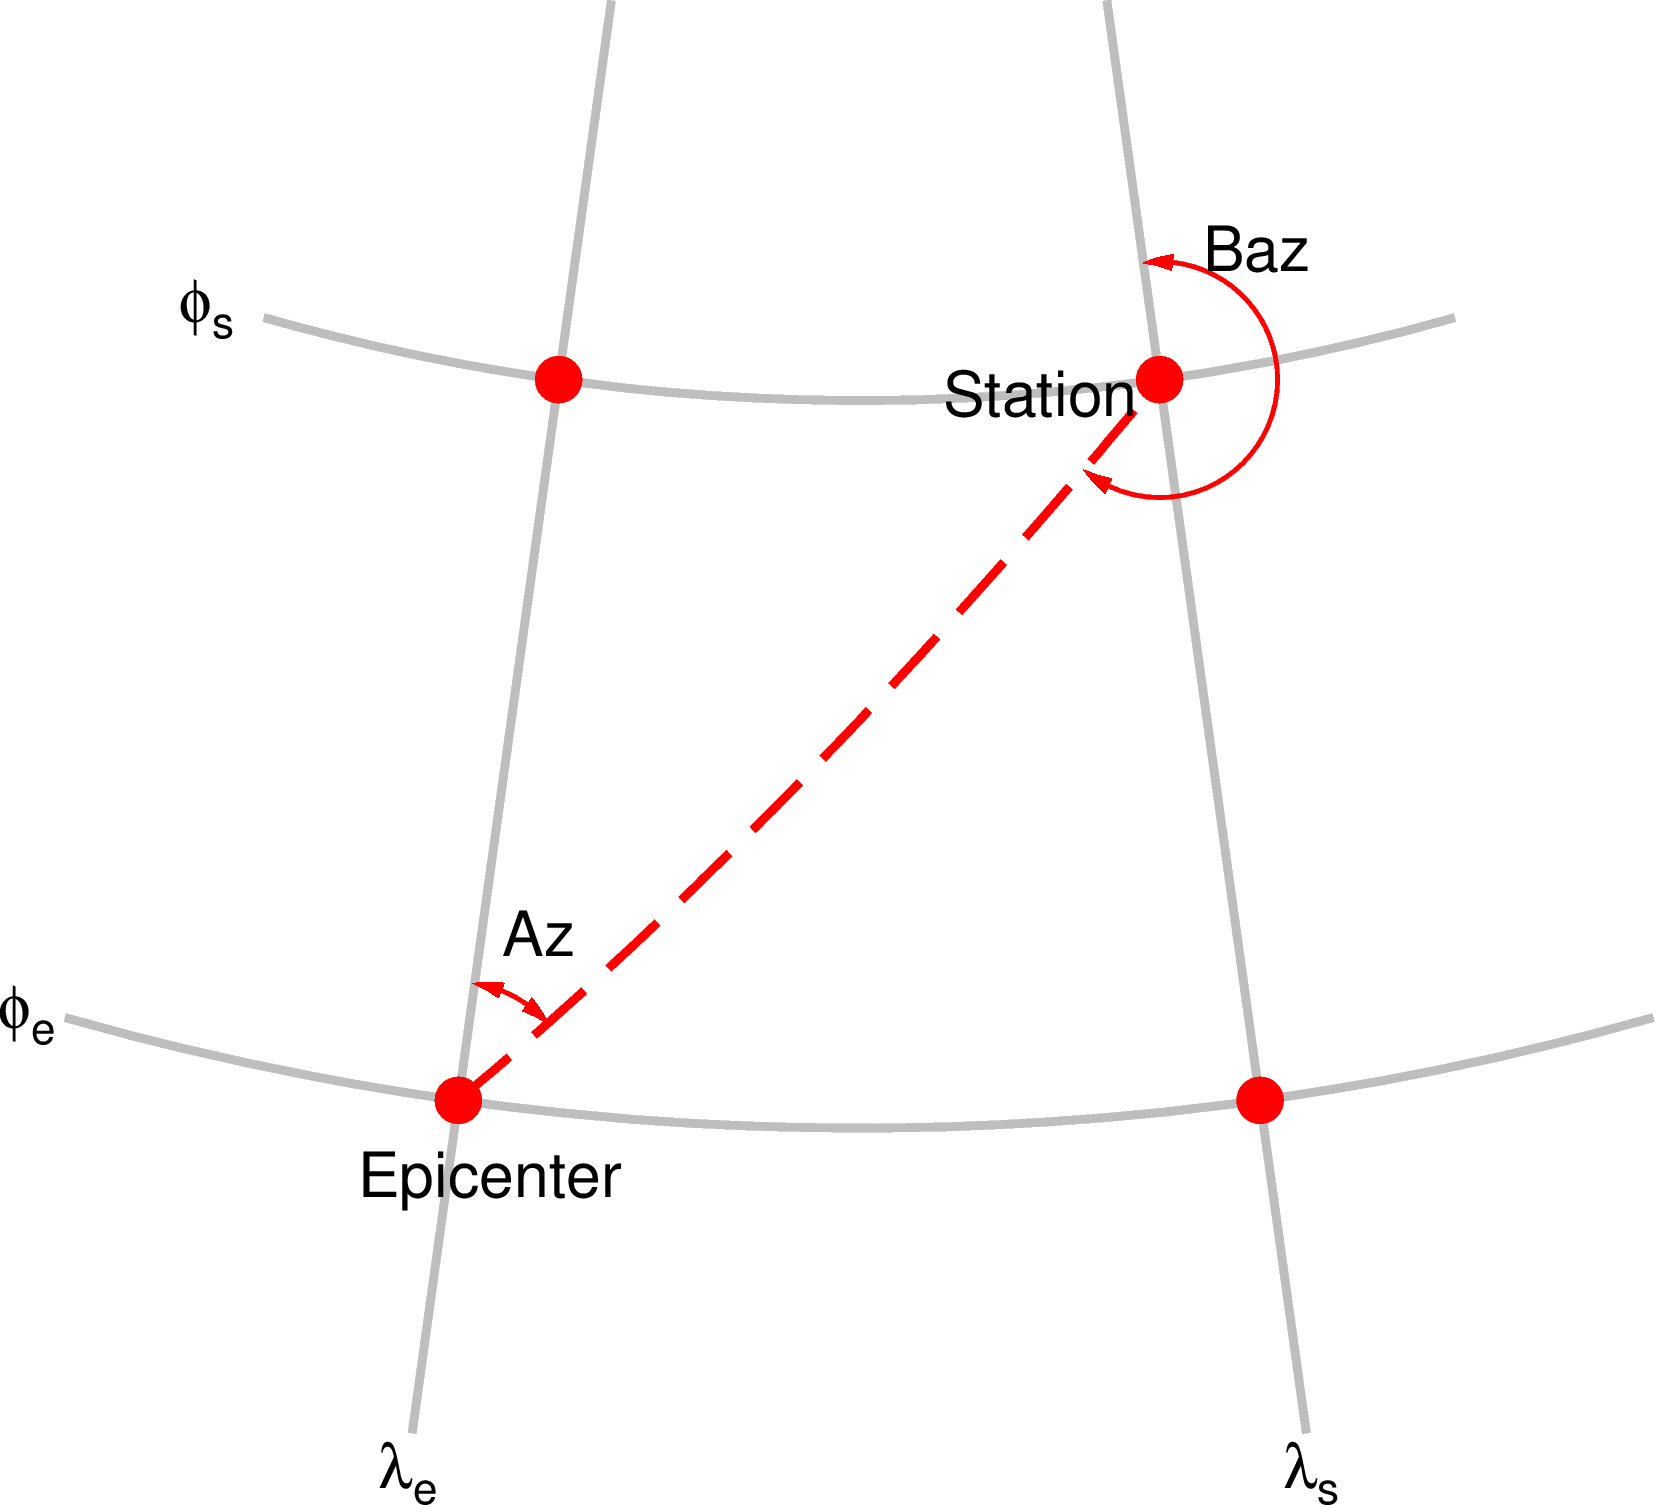
\includegraphics[width=8cm]{az-baz}
\caption[震中距、方位角、反方位角示意图]{震中距、方位角、反方位角示意图。}
\label{fig:gcarc-dist-az-baz}
\end{figure}

震中距、方位角和反方位角的计算涉及到球面三角的知识,具体公式及其推导可以参考相关书籍。此处仅提供一些参考:

\begin{itemize}
\item \url{http://www.eas.slu.edu/People/RBHerrmann/Courses/EASA462/}
\item \url{http://www.seis.sc.edu/software/distaz/}
\item SAC源码~\verb+src/ucf/distaz.c+
\item CPS330\footnote{\url{http://www.eas.slu.edu/eqc/eqccps.html}}源码~\verb+VOLI/src/udelaz.c+
\end{itemize}

\subsubsection{\texttt{o, ko}}
o为事件的发生时刻相对于参考时刻的秒数。ko是绘图时变量o的标识符。

\subsubsection{\texttt{khole}}
若为核爆事件,则其为孔眼标识;若为其它事件,则为位置标识。

\subsubsection{\texttt{nevid, norid, nwfid}}
三者分别标识事件ID、起始时间ID和波形ID,仅用于CSS 3.0文件中。CSS 3.0
是SAC可以处理的一种数据格式,应该是当初SAC商业化的产物,目前仍保留
在SAC头段中。

\subsection{台站相关变量}
\subsubsection{\texttt{knetwk, kstnm}}
地震台网名和台站名。

\subsubsection{\texttt{istreg}\dag}
台站地理区域。

\subsubsection{\texttt{stla, stlo, stel, stdp}}
台站纬度(-90到90度)、经度(-180到180度)、高程(单位m,目前未使用)、
相对地表的深度(单位m,目前未使用)。

\subsubsection{\texttt{cmpaz, cmpinc, kcmpnm, kstcmp}}
一个台站至少需要三个正交的通道(或分量)才能完整地记录地面运动物理量。cmpaz和cmpinc
指定了单个通道记录的方向矢量。

图~\ref{fig:cmpaz-cmpinc}~给出了SAC所使用的NEU坐标系,需要注意的是这是一个左手坐标系。
图中蓝色箭头为通道所记录的方向矢量,若地面运动与该方向一致,则为正,否则为负。
其中,头段变量cmpaz表征通道的方位角,其定义为从N向开始顺时针旋转的角度,即图中的角度$\phi$;
cmpinc表征通道的入射角,定义为U向向下旋转的度数,即图中的角度$\theta$。

\begin{figure}[H]
\centering
\tdplotsetmaincoords{55}{50}
\pgfmathsetmacro{\rvec}{.8}
\pgfmathsetmacro{\thetavec}{30}
\pgfmathsetmacro{\phivec}{30}
\begin{tikzpicture}[scale=5,tdplot_main_coords]
\coordinate (O) at (0,0,0);
\draw[thick,->] (0,0,0) -- (1,0,0) node[anchor=south west]{$E$};
\draw[thick,->] (0,0,0) -- (0,1,0) node[anchor=south]{$N$};
\draw[thick,->] (0,0,0) -- (0,0,1) node[anchor=north east]{$U$};

\tdplotsetcoord{P}{\rvec}{\thetavec}{\phivec}
\draw[-stealth,color=blue] (O) -- (P);
\draw[dashed, color=red] (O) -- (Pxy);
\draw[dashed, color=red] (P) -- (Pxy);

\tdplotdrawarc{(O)}{0.2}{\phivec}{90}{anchor=west}{$\phi$}

\tdplotsetthetaplanecoords{\phivec}
\tdplotdrawarc[tdplot_rotated_coords]{(0,0,0)}{0.5}{0}%
{\thetavec}{anchor=south west}{$\theta$}
\end{tikzpicture}
\caption{cmpaz和cpminc示意图}
\label{fig:cmpaz-cmpinc}
\end{figure}

根据定义,地震仪标准通道的cmpinc和cmpaz值如下表:
\begin{table}[H]
\caption{标准地震通道的cmpaz和cpminc}
\label{table:neu-cmpaz-cmpinc}
\centering
\begin{tabular}{ccc}
\toprule
方向    &   CPMAZ   &   CPMINC      \\
\midrule
N       &   0       &   90          \\
E       &   90      &   90          \\
U       &   0       &   0           \\
\bottomrule
\end{tabular}
\end{table}

对于非标准方向的地震通道来说,很容易根据cmpinc和cmpaz的值,将其旋转到NEU坐标系或者
RTZ坐标系,这些将在``\nameref{sec:traces-rotating}''一节中说到。

\verb+kcmpnm+用于存储分量名称。SEED格式规定通道名的三个字符中的最后一个代表通道的分量
方位,比如通道名~\verb+BHE+表示该通道为东西向。通常~\verb+kcmpnm+可以取为E、N、Z。
由于很多台站的水平分量并不严格是东西、南北方向,因而现在更倾向于用1和2代替N和E。

\verb+kstcmp+为辅助型变量,表示台站分量,由kstnm、cmpaz、cmpinc推导得到。

\subsubsection{\texttt{lpspol}}
如图~\ref{fig:cmpaz-cmpinc}~所示,在左手坐标系下,若三通道都是正极性则为真,否则为假。

\subsection{震相相关变量}
\subsubsection{\texttt{a, f, tn}}
a和f用于存储事件的初动时刻和结束时刻相对于参考时刻的秒数。

tn(n=0-9)用于存储用户自定义的时刻相对于参考时刻的秒数,常用于存储震相到时。

\subsubsection{\texttt{ka, kf, ktn}}
a、f以及tn都有一个对应的以k开头的字符型头段变量,称之为时间标识。时间标识用于说明
对应的时间头段变量中所包含时间的含义。

比如头段变量a中通常包含P波到时,则此时ka的值可以设置为P;头段变量t1中包含了震相
PcP的到时,则一般定义kt1为``PcP''。

在绘图时,若时间头段变量中有值,则默认会在该时刻处绘制一条垂线,若相应的时间标记
有定义,则将时间标记的值显示在垂线附近。

\subsubsection{\texttt{Xmarker}}
震相相关的变量对可以构成一个辅助型变量。a和ka可以构成amarker,f和kf可以构成fmarker,
o和ko可以构成omarker,tn和ktn可以构成tnmarker(n=0-9)。

这些辅助型变量可以在~\nameref{cmd:listhdr}中使用。

\subsection{仪器相关变量}
\subsubsection{\texttt{kinst}, \texttt{iinst}\dag, \texttt{respn}\dag}
kinst为记录仪器的通用名称,iinst为记录仪器的类型,respn为仪器相应参数。

\subsection{其它变量}
\subsubsection{\texttt{usern, kusern}}
usern(n=0-9)和kusern(n=0-2)均用来存储用户自定义值。不像a和ka那样成对存在,
usern和kusern之间没有对应关系。比如可以将波形的信噪比保存在user0中,将任意字符串
保存到kuser0中。

\subsubsection{\texttt{lovrok}}
若为~\verb+TRUE+,则磁盘里的原始数据可被覆盖;若为~\verb+FALSE+,则原始数据不可被覆盖。
主要用于保护原始数据,一般来说很少用到,若是出于保护原始数据的目的,
应优先考虑对原始数据做备份。

\subsubsection{\texttt{lcalda}}
全称为Calculate Distance and Azimuth。若为~\verb+TRUE+,则当事件和台站的坐标被
写入或被修改时,头段变量dist、gcarc、az、baz将自动计算;否则dist、gcarc、az、baz
不会被自动计算,SAC头段中会存在信息的不兼容。

\subsubsection{\texttt{kdatrd}}
数据被读入计算机的日期(一般很少使用)。

\section{SAC中的时间概念}
\label{sec:sac-time}

\subsection{基本思路}
SAC的头段区有很多与时间相关的头段变量,包括 \texttt{nzyear}、
\texttt{nzjday}、\texttt{nzhour}、\texttt{nzmin}、\texttt{nzsec}、
\texttt{nzmsec}、\texttt{b}、\texttt{e}、\texttt{o}、\texttt{a}、
\texttt{f}、\texttt{tn}(n=0--9)。
正确使用它们的前提是理解SAC中的时间概念。这一节将试着说清楚这个问题。

首先,SAC处理的是地震波形数据,SAC格式里保存的是时间序列数据。先不管
其它的一些台站经纬度、事件经纬度信息,就数据而言,至少需要一系列数据值
以及每个数据值所对应的时刻。

在本节接下来的内容中,将严格区分两个高中物理学过的概念:时刻和时间。
简单地说,在时间轴上,时刻是一个点,时间是一个线段。

一个简单的例子如下:
\begin{verbatim}
        2014-02-26T20:45:00.000     0.10
        2014-02-26T20:45:01.000     0.25
        2014-02-26T20:45:02.000     0.33
        2014-02-26T20:45:03.000     0.21
        2014-02-26T20:45:04.000     0.35
        2014-02-26T20:45:05.000     0.55
        2014-02-26T20:45:06.000     0.78
        2014-02-26T20:45:07.000     0.66
        2014-02-26T20:45:08.000     0.42
        2014-02-26T20:45:09.000     0.34
        2014-02-26T20:45:10.000     0.25
\end{verbatim}
其中第二列是数据点,每个数据点所对应的时刻放在第一列,格式为
``\texttt{yyyy-mm-ddThh:mm:ss.xxx}''。数据点是以 \SI{1}{\s} 的等间隔
进行采样的。

若把这堆时刻以及数据点直接写入文件中,将占据大量的磁盘空间,读写也很
不方便。考虑将某一个时刻定义为参考时刻,并把其它所有的时刻都用相对于
该参考时刻的秒数来表示,这样可以简化不少。

比如取``\texttt{2014-02-26T20:45:00.000}''为参考时刻,即
\begin{verbatim}
        nzyear = 2014
        nzjday = 57
        nzhour = 20
        nzmin  = 45
        nzsec  = 00
        nzmsec = 000
\end{verbatim}
则上面的数据可以简化为
\begin{verbatim}
        00.000     0.10
        01.000     0.25
        02.000     0.33
        03.000     0.21
        04.000     0.35
        05.000     0.55
        06.000     0.78
        07.000     0.66
        08.000     0.42
        09.000     0.34
        10.000     0.25
\end{verbatim}
其中第二列是数据点,第一列是每个数据点对应的时刻相对于参考时刻的相对时间,
下面简称其为相对时间。

显然参考时刻的选取是任意的,若取``\texttt{2014-02-26T20:45:05.000}''为
参考时刻,则上面的数据简化为
\begin{verbatim}
        -05.000     0.10
        -04.000     0.25
        -03.000     0.33
        -02.000     0.21
        -01.000     0.35
         00.000     0.55
         01.000     0.78
         02.000     0.66
         03.000     0.42
         04.000     0.34
         05.000     0.25
\end{verbatim}

一般来说,会选取一个比较特殊的时刻作为参考时刻,比如第一个数据点对应的
时刻,或者地震波形数据中的发震时刻。

下面还是回到以``\texttt{2014-02-26T20:45:00.000}''为参考时刻简化得到的结
果。因为数据是等间距的,相对时间这一列完全可以进一步简化,比如用``起始相
对时间+采样间隔+数据点数''或者``起始相对时间+采样间隔+结束相对时间''就完
全可以表征第一列的相对时间。

SAC选择了另外一种简化模式,``起始相对时间+采样间隔+数据点数+结束相对时间'',
即头段变量中的``\texttt{b+delta+npts+e}'',这其实是存在信息冗余的,这就
造就了头段变量 \texttt{e} 的一些特殊性,后面会提到。

按照SAC的模式在对相对时间进行简化之后,整个数据可以表示为
\begin{verbatim}
        nzyear = 2014
        nzjday = 57
        nzhour = 20
        nzmin  = 45
        nzsec  = 00
        nzmsec = 000
        b      = 0.0
        e      = 10.0
        delta  = 1.0
        npts   = 11

        0.10
        0.25
        0.33
        0.21
        0.35
        0.55
        0.78
        0.66
        0.42
        0.34
        0.25
\end{verbatim}
似乎到这里就结束了。

地震学里的一个重要问题是拾取震相到时(时刻),所以还需要几个额外的
头段变量来保存这些震相到时(时刻),不过显然不需要真的把``时刻''保存
到这些头段变量中,不然上面的一大堆就真是废话了。SAC将震相到时(时刻)
相对于参考时刻的时间差(即相对时间)保存到头段变量 \texttt{o}、
\texttt{a}、\texttt{f}、\texttt{tn} 中。

综上,SAC中跟时间有关的概念有三个:
\begin{description}
\item [参考时刻] 由头段变量 \texttt{nzyear}、\texttt{nzjday}、
    \texttt{nzhour}、\texttt{nzmin}、\texttt{nzsec}、\texttt{nzmsec} 决定
\item [相对时间] 即某个时刻相对于参考时刻的时间差(单位为秒),保存到
    头段变量 \texttt{b}、\texttt{e}、\texttt{o}、\texttt{a}、\texttt{f}、
    \texttt{tn}(n=0--9)
\item [绝对时刻] =参考时刻+相对时间
\end{description}

\subsection{一些测试}
下面以一个具体的数据为例,通过修改各种与时间相关的头段来试着去进一步
理解SAC的时间概念。

\subsubsection{生成样例数据}
\begin{SACCode}
SAC> fg seis
SAC> lh iztype
    iztype = BEGIN TIME
SAC> ch iztype IUNKN
SAC> w seis
\end{SACCode}
\texttt{lh} 是命令 \nameref{cmd:listhdr} 的简写,用于列出头段变量的值。
\texttt{ch} 是 \nameref{cmd:chnhdr} 的简写,用于修改头段变量的值。这里
额外多做了一个操作修改 \texttt{iztype} 的操作,这是由于这个数据稍稍有
一点bug。

\texttt{iztype} 指定了参考时刻的类型,其显示为 \texttt{BEGIN TIME},
实际上其枚举值是 \texttt{IB},也就是说这个数据选取文件第一个数据点的
时刻作为参考时刻,那么 \texttt{b} 的值应该为0。而实际上这个数据的
\texttt{b} 值并不为0,这其实是这个数据的一点小bug。这也从另一个侧面说明
SAC只有在修改与时间相关的头段变量时才可能会检查到这个错误/警告,所以这里
先将其修正为 \texttt{IUNKN}。

\subsubsection{修改文件起始时间b}
\begin{SACCode}
SAC> r seis
SAC> lh kzdate kztime b delta npts e o a f

     kzdate = MAR 29 (088), 1981
     kztime = 10:38:14.000
          b = 9.459999e+00
      delta = 1.000000e-02
       npts = 1000
          e = 1.945000e+01
          o = -4.143000e+01
          a = 1.046400e+01
SAC> ch b 10
SAC> lh

     kzdate = MAR 29 (088), 1981
     kztime = 10:38:14.000
          b = 1.000000e+01
      delta = 1.000000e-02
       npts = 1000
          e = 1.999000e+01
          o = -4.143000e+01
          a = 1.046400e+01
\end{SACCode}

修改 \texttt{b} 前后的变化仅在于 \texttt{b} 和 \texttt{e} 值的变化,而
参考时刻以及其它相对时间并没有发生变化。

这意味着整段SAC数据中的任意一个数据点所对应的时刻\footnote{好长的修饰语}
都向后延迟了0.54秒!这样做很危险,因为 \texttt{b} 和 \texttt{e} 的绝对
时刻被修改了,而其它头段如 \texttt{o}、\texttt{a}、\texttt{f}、
\texttt{tn} 的绝对时刻却没有变。

使用的时候必须非常小心:
\begin{itemize}
\item 如果 \texttt{o}、\texttt{a}、\texttt{f}、\texttt{tn} 都没有定义,
    那么修改 \texttt{b} 值可以用于校正仪器的时间零飘\footnote{零飘,即
    仪器中的时刻与标准时刻不同。}以及时区差异\footnote{时区差异可以理
    解成另一种零飘。}。关于时区的校正,参考``\nameref{sec:time-zone-correction}''
    一节。
\item 如果 \texttt{o}、\texttt{a}、\texttt{f}、\texttt{tn} 已经被定义,
    则修改 \texttt{b} 值会导致与震相相关的头段变量出现错误!\footnote{
    如果只定义了 \texttt{o} 值,或者 \texttt{a}、\texttt{f}、\texttt{tn}
    为理论震相到时而非计算机拾取或人工拾取的到时,修改 \texttt{b} 也是
    没有问题的。有些乱,不多说了。总之不要随便修改 \texttt{b} 的值。}
\end{itemize}

\subsubsection{修改文件结束时间e}
\begin{SACCode}
SAC> r ./seis
SAC> lh kzdate kztime b delta npts e o a f

     kzdate = MAR 29 (088), 1981
     kztime = 10:38:14.000
          b = 9.459999e+00
      delta = 1.000000e-02
       npts = 1000
          e = 1.945000e+01
          o = -4.143000e+01
          a = 1.046400e+01
SAC> ch e 0
SAC> lh

     kzdate = MAR 29 (088), 1981
     kztime = 10:38:14.000
          b = 9.459999e+00
      delta = 1.000000e-02
       npts = 1000
          e = 1.945000e+01
          o = -4.143000e+01
          a = 1.046400e+01
\end{SACCode}

可以看到,修改前后所有变量均没有发生变化,即 \texttt{e} 的值是不可以
随意改变的,根据上面的结果可知,\texttt{e} 的值是通过 \texttt{b}、
\texttt{delta}、\texttt{npts}的值动态计算的。这也与上一节说到的头段变量
冗余问题相符合。不要试图修改 \texttt{delta}、\texttt{npts},这不科学!

\subsubsection{修改o、a、f、tn}
这几个头段变量完全是由用户自定义的,因而任何的定义、修改、取消定义都
不会对数据的正确性产生影响,因而这里不再测试。

\subsubsection{修改参考时间}
\begin{SACCode}
SAC> r ./seis
SAC> lh kzdate kztime b delta npts e o a f

     kzdate = MAR 29 (088), 1981
     kztime = 10:38:14.000
          b = 9.459999e+00
      delta = 1.000000e-02
       npts = 1000
          e = 1.945000e+01
          o = -4.143000e+01
          a = 1.046400e+01
SAC> ch nzsec 15
SAC> lh

     kzdate = MAR 29 (088), 1981
     kztime = 10:38:15.000
          b = 9.459999e+00
      delta = 1.000000e-02
       npts = 1000
          e = 1.945000e+01
          o = -4.143000e+01
          a = 1.046400e+01
\end{SACCode}

试图修改参考时刻,整个SAC头段,除了参考时刻外其它时间变量都没有发生变化。
根据``绝对时刻=参考时刻+相对时间''可知,这导致所有SAC数据点的绝对时刻
发生了平移,这一点理论上可以用于校正零飘或者时区,但是由于SAC不支持智能
判断时间(比如不知道1时80分实际上是2时20分),所以修改时区时需要获取
参考时刻6个头段变量,加上时区的校正值,再写入到参考时刻6个变量中,相对
较为繁琐,因而若要校正时区,建议直接修改头段变量中的 \texttt{b} 值。

\subsubsection{修改发震时刻}
数据处理中一个常见的需求是修改发震时刻,这可以通过修改头段变量 \texttt{o}
来实现,但是经常需要将参考时刻设置为发震时刻。上面的测试表明,直接修改
参考时刻是很危险的,所以SAC的 \texttt{ch} 命令提供了 \texttt{allt} 选项来
实现这一功能,在``\nameref{sec:event-info}''一节中会具体解释。

\subsection{总结}
将SAC中的时间变量分为三类:
\begin{enumerate}
\item 参考时刻:即 \texttt{nzyear}、\texttt{nzjday}、\texttt{nzhour}、
    \texttt{nzmin}、\texttt{nzsec}、\texttt{nzmsec};
\item 相对时间:即\texttt{o}、\texttt{a}、\texttt{f}、\texttt{tn};
\item 特殊的相对时间:即\texttt{b}\footnote{由于e不可独立修改,所以不再考虑};
\end{enumerate}

第二类时间变量可以随意修改,即震相拾取。

第一、三类时间变量的修改会导致数据绝对时刻发生改变。一般通过修改第三类
时间变量来校正时间零漂和时区差异。在设置了发震时刻后,应使用
\nameref{cmd:chnhdr} 命令的 \texttt{allt} 选项修改第一、三类时间变量。


\chapter{SAC数据处理}
\label{chap:data-process}
\input{data-process/intro-to-process}
\input{data-process/data-request}
\input{data-process/data-format}
\section{合并数据}
相关命令: \nameref{cmd:merge}

有些时候,从SEED数据中解压出来的同一台站同一分量的连续波形数据,
会被切割成多个等长或不等长的文件,数据断开的可能原因是仪器在某些时刻存在问题导致
连续数据出现间断,也可能是出于其它考虑将数据进行切割。此时需要首先对数据进行合并。

假定解压出来的台网NET、台站STA、位置为00的BHZ分量的连续波形被分割成了多个文件,
需要将多个文件合并成单个文件。

对于v101.6之前的版本,只能用如下命令进行合并:
\begin{SACCode}
SAC> r 2012.055.12.00.00.0000.NET.STA.00.BHZ.Q.SAC
SAC> merge 2012.055.12.25.00.0000.NET.STA.00.BHZ.Q.SAC
SAC> merge 2012.055.12.40.00.0000.NET.STA.00.BHZ.Q.SAC
SAC> ...
SAC> merge 2012.055.13.20.00.0000.NET.STA.00.BHZ.Q.SAC
SAC> w NET.STA.00.BHZ
\end{SACCode}
即先读取第一段数据,然后合并第二段数据,再合并第三段数据,对于多个数据段的合并,
需要执行多次合并命令,且合并时需要遵循文件的先后顺序。

SAC从v101.6开始重写了 \nameref{cmd:merge} 命令,可以使用如下更简洁的形式:
\begin{SACCode}
SAC> r *.NET.STA.00.BHZ        // 读入所有需要合并的文件
SAC> merge                     // 内存中的所有文件被合并为一个文件
SAC> w NET.STA.00.BHZ          // 写回到磁盘中
\end{SACCode}

当然,SAC v101.6还提供了更简洁的形式:
\begin{SACCode}
SAC> merge *.NET.STA.00.BHZ     // 读取需要合并的文件,并合并
SAC> w NET.STA.00.BHZ           // 写回到磁盘
\end{SACCode}

对于所有要合并的数据文件,SAC会检测其knetwk、kstnm、kcmpnm和delta是否完全匹配,并
智能判断每个文件的合并顺序。

实际合并的过程中,可能会出现数据间断或数据重叠的情况。若数据存在间断,可对其直接
补零或线性插值;若数据存在重叠,则可以比较重叠部分数据是否相同或对重叠的波形进行平均。

\section{数据重命名}
用rdseed软件从SEED格式中解压得到的SAC数据,一般都具有固定格式的文件名。
示例如下:
\begin{minted}{bash}
2012.055.12.34.56.7777.YW.MAIO.01.BHE.Q.SAC
2012.055.12.34.50.6666.YW.MAIO.01.BHN.Q.SAC
2012.055.12.34.54.5555.YW.MAIO.01.BHZ.Q.SAC
\end{minted}
这三个文件是YW台网MAIO台站的宽频地震仪记录的宽频带三分量(BHE、BHN、BHZ)波形数据。
文件名中每一项的具体含义在``\nameref{chap:naming}''中有介绍,这里不再重复。

默认的文件名比较长,在数据处理时可能会显得比较麻烦,一般都会根据实际需求进行适当的简化。

是否要对数据文件做重命名,以及按照什么格式重命名,都是没有固定的标准的。通常需要
用户根据自己所做研究的实际情况来决定。

在某些情况下,我们会将同一事件在所有台站的波形数据放在同一个文件夹下,并将文件名以事件的
发生日期/时间来命名。那么,SAC文件名中的时间等信息就可以被省略掉。数据文件名简化为:
\begin{minted}{bash}
YW.MAIO.BHE
YW.MAIO.BHN
YW.MAIO.BHZ
\end{minted}

有时候,我们会将不同事件在同一个台站的波形数据放在同一个文件夹下,并将文件名以台站
名来命名,此时数据文件名中可能需要保留事件的日期信息。数据文件名可以简化为:
\begin{minted}{bash}
YW.MAIO.20120224.BHE
YW.MAIO.20120224.BHN
YW.MAIO.20120224.BHZ
\end{minted}

数据重命名这一步骤可以单独执行,也可以在执行其他操作的过程中顺便进行重命名(比如将
数据合并并写入磁盘的时候)。通常需要写脚本来完成重命名的操作,重命名脚本的Bash版本
位于第 \pageref{subsec:rename-in-bash} 页,Perl版本位于第 \pageref{subsec:rename-in-perl} 页,
Python版本位于第 \pageref{subsec:rename-in-python} 页。

\input{data-process/time-zone-correction}
\section{事件信息}
\label{sec:event-info}
相关头段:evla, evlo, evdp, mag, o, nzyear, nzjday, nzhour, nzmin, nzsec, nzmsec

一般来说,从SEED连续波形中解压得到的SAC数据中是没有事件信息的。这就需要用户从
地震目录中获取事件的发震时刻、经度、纬度、深度和震级信息,并将这些信息写入到
SAC文件的头段中。SAC提供了用于可以修改头段变量的命令 \nameref{cmd:chnhdr},
以及将修改后的头段变量写到磁盘文件的命令 \nameref{cmd:writehdr}
\footnote{
也可以使用``\texttt{w over}''将修改写回磁盘文件。二者的区别在于,``\texttt{wh}''
仅仅覆盖磁盘文件的头段区,而``\texttt{w over}''则覆盖整个文件。这里使用``\texttt{wh}''
是因为此处只修改了头段区,而没有对数据做任何修改,使用``\texttt{wh}''即可满足要求,
且从执行效率上看``\texttt{wh}''比``\texttt{w over}''要快不少。}。

\subsection{经纬度、深度与震级}
想要修改事件的经纬度、深度和震级,操作如下:
\begin{SACCode}
SAC> r cdv.?
SAC> ch evla 37.52 evlo -121.68 evdp 5.95   // 修改三个头段变量
SAC> ch mag 5.0                             // 修改一个头段变量
SAC> wh                                     // 将修改后的头段写入文件
\end{SACCode}

\subsection{发震时刻}
通常,需要将发震时刻信息写入SAC头段,并设置SAC文件的参考时刻为发震时刻。
这样设置的好处在于,可以直观地从X轴坐标上读取震相走时。要实现这一操作,需要
用到 \nameref{cmd:chnhdr} 的两个特殊用法。

假设发震时刻为1987年06月22日11时10分10.363秒:
\label{code:origin-time}
\begin{SACCode}
SAC> r ./cdv.?
SAC> ch o gmt 1987 173 11 10 10 363   // 06月22日是第173天
SAC> lh kzdate kztime o

     kzdate = JUN 22 (173), 1987
     kztime = 11:09:56.363
          o = 1.400000e+01       // 发震时刻相对于参考时刻的时间为14秒
SAC> ch allt -14 iztype IO       // 参考时间加14秒,其他时间减14秒
SAC> lh kzdate kztime o

     kzdate = JUN 22 (173), 1987
     kztime = 11:10:10.363
          o = 0.000000e+00
SAC> wh                          // 写回磁盘
\end{SACCode}

在上面的例子中,首先从地震目录中获取了地震的发震时刻,然后计算发震日期对应一年中的第几天,
本例中为第173天,再利用``\texttt{ch o gmt yyyy ddd hh mm sss xxx}''
的语法将发震时刻赋值给头段变量 \texttt{o},SAC会自动将发震时刻转换为相对于
参考时刻的相对时间。由于此时SAC文件的参考时刻为``1987-06-22T11:09:56.363'',
而o值对应的时刻为发震时刻``1987-06-22T11:10:10.363'',所以头段变量o的值为发震时刻
相对于参考时刻的时间差,即14s。

将发震时刻写入头段之后,还需要将参考时刻修改为发震时刻,与此同时还要修改所有的相对时间。
``\texttt{ch allt xx.xx}''的功能是将所有已定义的相对时间加上 \texttt{xx.xx} 秒,
同时从参考时刻中减去 \texttt{xx.xx} 秒,此时参考时刻即为发震时刻,而o值为 \texttt{0}。

实际数据处理的时候,不可能像上面的示例那样使用``\texttt{lh o}''查看o的值再使用
``\texttt{ch allt}''选项,此时就需要使用SAC提供的引用头段变量的值的功能。具体的语法
以及用法会在``\nameref{chap:sac-programming}''一章中介绍。

\begin{SACCode}
SAC> ch o gmt 1987 173 11 10 10 363
SAC> ch allt (0 - &1,o&) iztype IO
\end{SACCode}

需要注意,上例中的``\verb|(0 - &1,o&)|''必须原样输入!由于101.6版本重写了SAC宏
的语法分析器,所以很多用法都发生了改变。你可能会发现,在101.6及其以后的版本中,
\verb|(0-&1,o&)|、\verb|(-&1,o&)|、\verb|(-&1,o)| 都
可以正常使用,但是上例中的版本是唯一一个在所有SAC版本中都正确的,为了命令的通用性,
只要记住这个就可以了。

进行实际数据处理时,可以参考第 \ref{call:ch-orign} 节中提供的Perl脚本。

\section{台站和分量信息}
相关头段:stla、stlo、cmpaz、cmpinc

一般来说,从SEED数据中解压的SAC数据中都包含了准确的台站信息和分量信息。若数据中
没有包含台站和分量信息,则需要从其它途径获取这些信息,
并使用 \nameref{cmd:chnhdr} 将这些信息写入到相应的数据头段中。

\section{去毛刺}
相关命令:\nameref{cmd:rglitches}

地震仪器偶尔会出现问题,导致连续地震数据流中出现尖锋或者数据丢失。
这些所谓的毛刺,肉眼很容易识别,但是在使用程序自动处理数据时却很容易被误认为是地震信号,
因而需要在数据分析之前将毛刺去除。\nameref{cmd:rglitches} 命令可以在某种程度上
检测并去除地震信号中的毛刺。毛刺在模拟地震记录中很常见,现在的数字地震记录中
则很少见到,因而实际上很少需要执行这一步操作。

\nameref{cmd:rglitches} 的效果可以从图 \ref{fig:deglitches} 中直观地看到。
\begin{figure}[H]
\centering
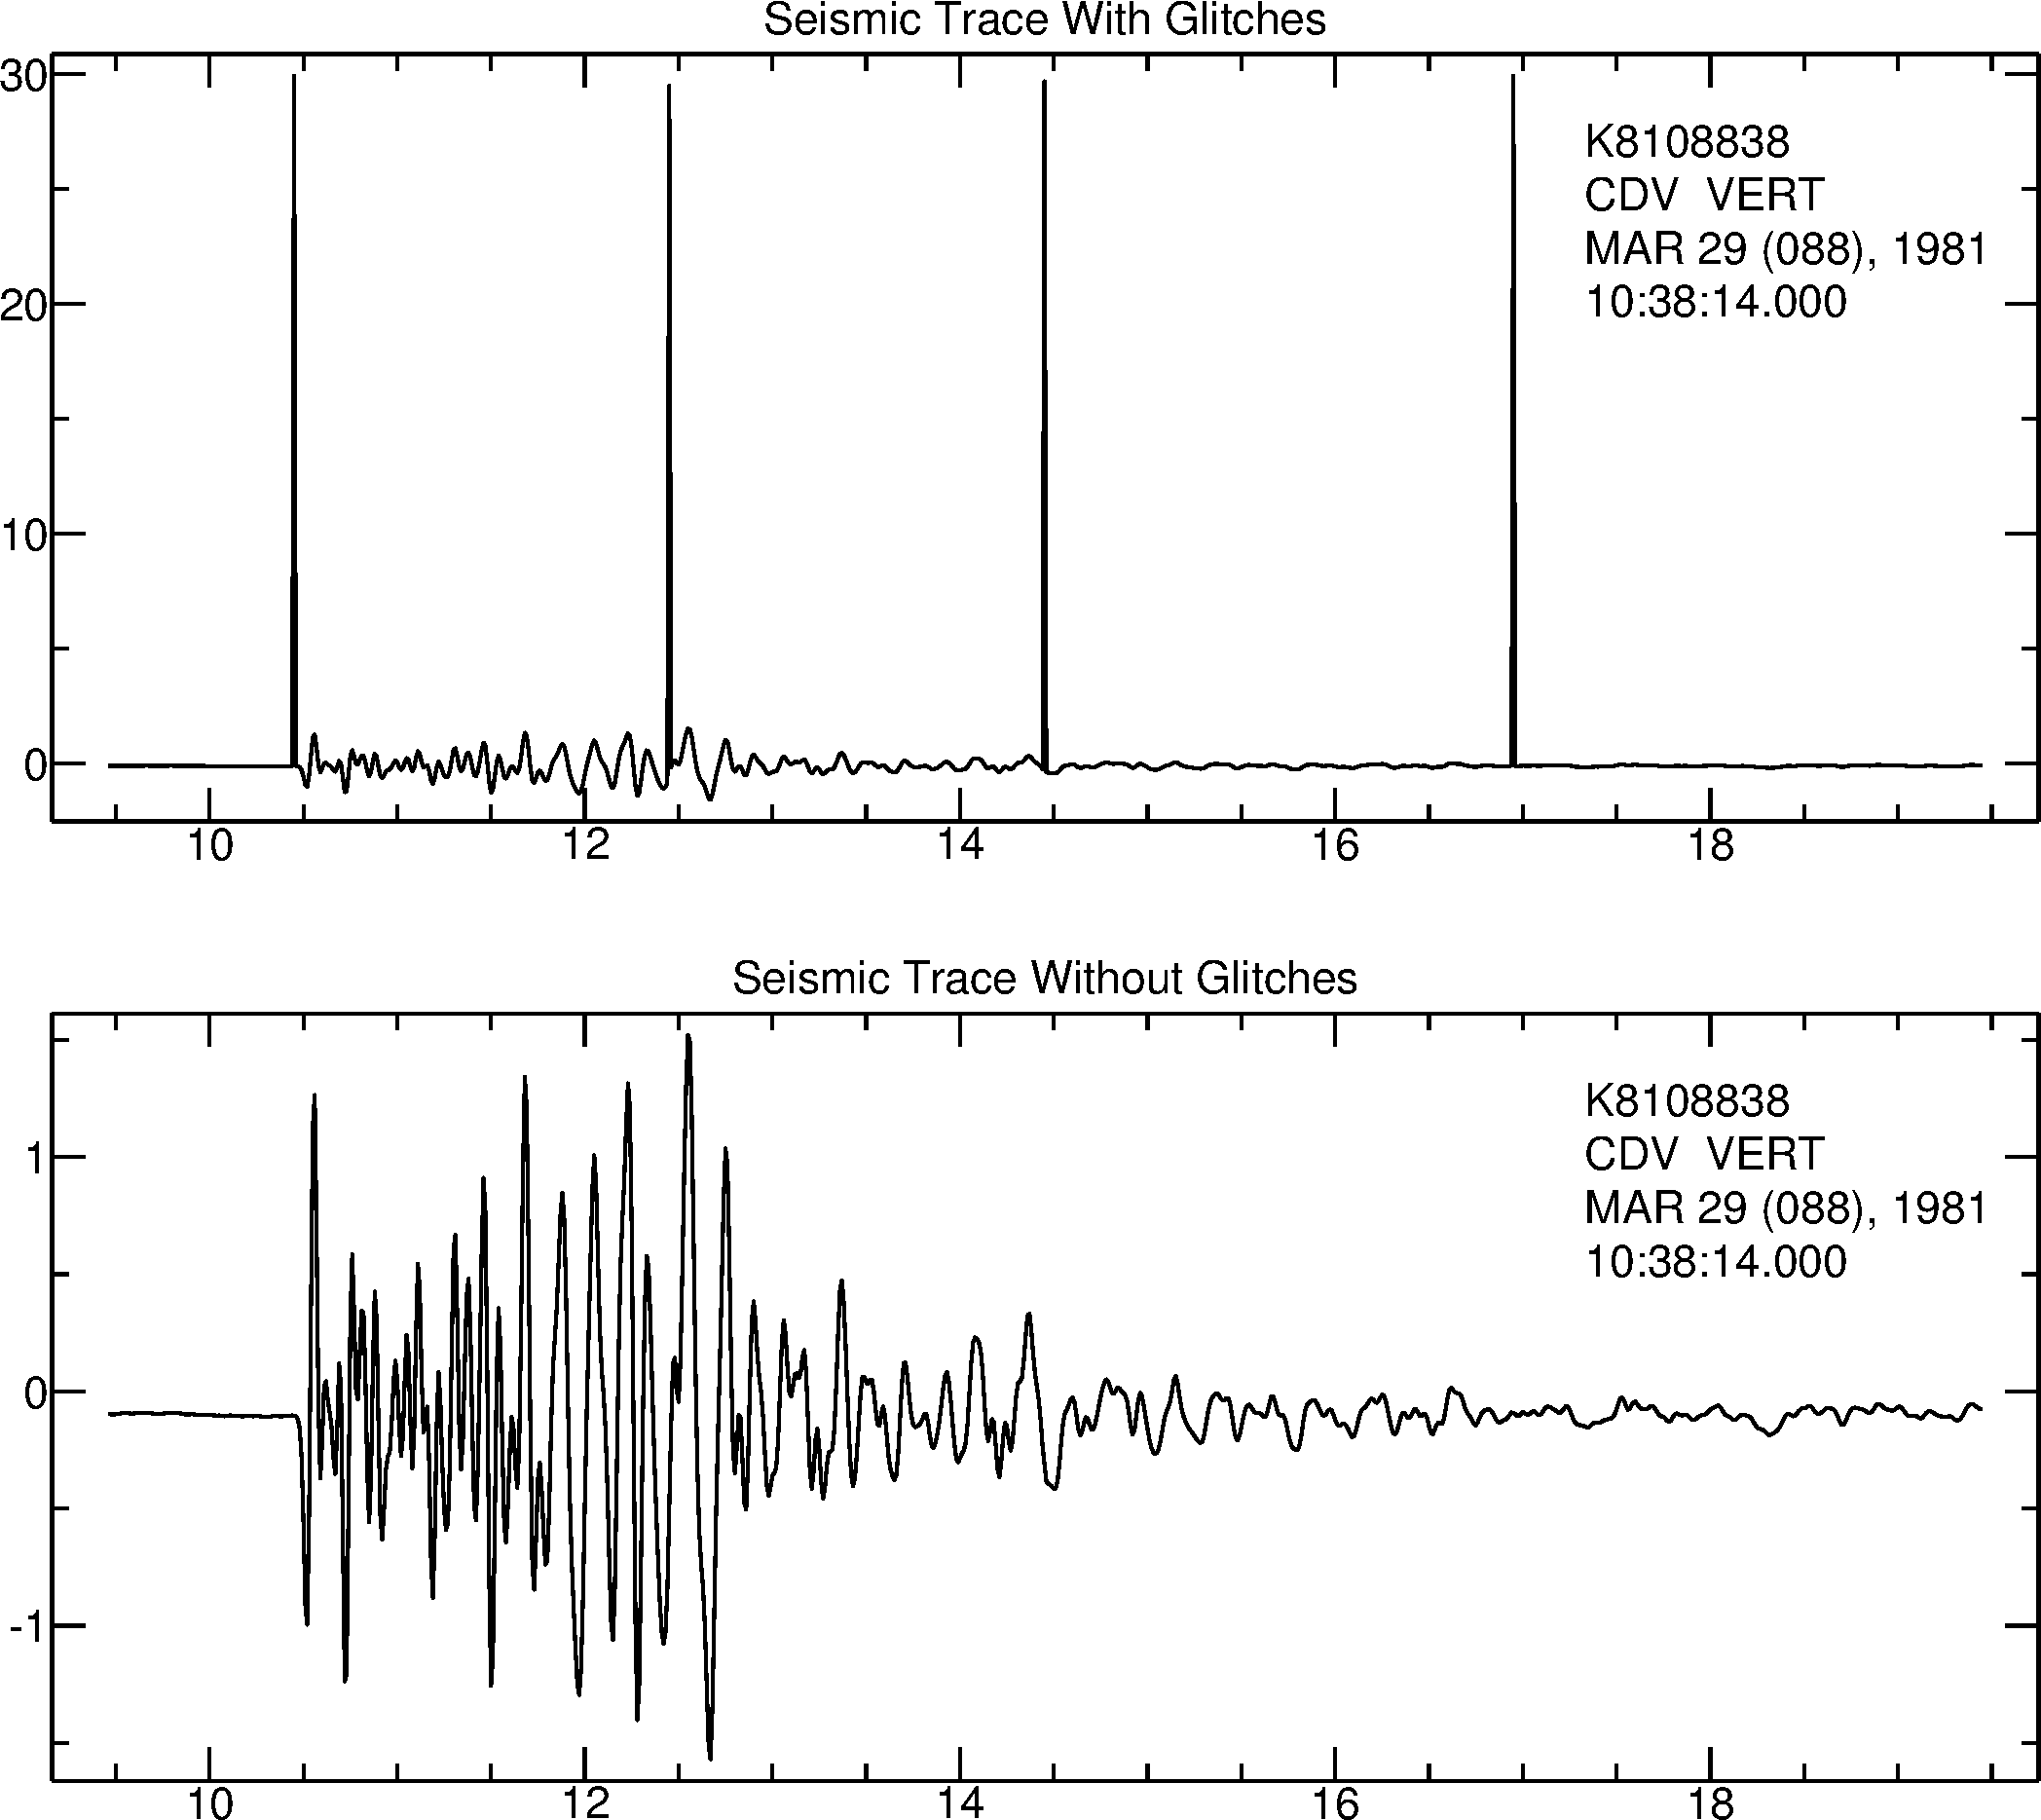
\includegraphics[width=0.95\textwidth]{rglitches}
\caption[地震波形去毛刺]{地震波形去毛刺。上图为包含glitches的地震信号,下图为去除
rglitches后的地震信号。}
\label{fig:deglitches}
\end{figure}

\section{数据重采样}
相关命令:\nameref{cmd:decimate}、\nameref{cmd:interpolate}

如下情形,需要对数据进行重采样:
\begin{itemize}
\item 不同仪器的采样周期可能不同,需要将所有的数据重采样到相同的采样周期;
\item 数据的采样周期很小,导致数据量很大,而实际研究中不需要如此小的采样周期,因而可以对数据做减采样以减小数据量;
\item 数据的采样周期过大,实际研究中需要更小的采样周期,此时需对数据做插值重采样;
\item 数据为不等间隔数据,需要插值成为等间隔数据;
\end{itemize}

\subsection{decimate}
\nameref{cmd:decimate} 专门用于解决上面所说的第二种情形,即等间隔数据的减采样。
在减采样过程中,根据Nyquist采样定理,可能会出现混叠现象,而 \nameref{cmd:decimate} 对
数据自动做了低通滤波,以避免混叠现象的产生。

下面的示例中,将一个等间隔数据,减采样10倍:
\begin{SACCode}
SAC> fg seis
SAC> lh delta npts

     delta = 1.000000e-02       //采样间隔delta=0.01
      npts = 1000
SAC> decimate 5; decimate 2     // 减采样10倍
SAC> lh delta npts

     delta = 9.999999e-02       //采样间隔delta=0.1,忽略浮点数误差
      npts = 100
\end{SACCode}

\subsection{interpolate}
与 \nameref{cmd:decimate} 相比,\nameref{cmd:interpolate} 命令功能更加强大,
其可以对等间隔或不等间隔数据进行增采样或减采样。

比如增采样,即插值:
\begin{SACCode}
SAC> fg seis
SAC> lh delta npts

     delta = 1.000000e-02
     npts = 1000
SAC> interp delta 0.005         // 增采样5倍
SAC> lh

     delta = 5.000000e-03
     npts = 1999
\end{SACCode}

对于减采样,\nameref{cmd:interpolate} 与 \nameref{cmd:decimate} 的功能略有重复,
但 \nameref{cmd:interpolate} 在减采样时不会对数据进行低通滤波,因而
使用 \nameref{cmd:interpolate} 进行减采样时可能会出现混叠现象,故而需要手动进行低通
滤波。

下面的示例将数据减采样到 \SI{20}{\Hz}。根据Nyquist采样定理,为了保证
不产生混叠现象,应首先对数据做 \SI{10}{\Hz} 的低通滤波。
\begin{SACCode}
SAC> fg seis
SAC> lh npts delta

     npts = 1000
     delta = 1.000000e-02
SAC> lp c 10
SAC> interpolate delta 0.05
WARNING potential for aliasing. new delta: 0.0500 data delta: 0.0100
    //  在做了lowpass之后,此处的警告可忽略
\end{SACCode}

\section{去均值、去线性趋势和波形尖灭}
相关命令:\nameref{cmd:rmean}、\nameref{cmd:rtrend}、\nameref{cmd:taper}

通常,波形数据总会存在一个非零的均值或者存在一个长周期的线性趋势,这会影响到数据
的分析,必须在数据分析前去除。另一方面,在对数据进行谱域操作(如FFT、滤波等)时,
若数据的两端不为零,则会出现谱域假象,因而实际数据经常需要做尖灭处理,
使得数据两端在短时间窗内逐渐变成零值。

\begin{SACCode}
SAC> fg seis
SAC> rmean; rtr; taper
\end{SACCode}

图 \ref{fig:rmean-rtrend-taper} 中,波形从上到下依次为原始波形、去均值、去线性趋势、和尖灭之后的波形。

\begin{figure}[H]
\centering
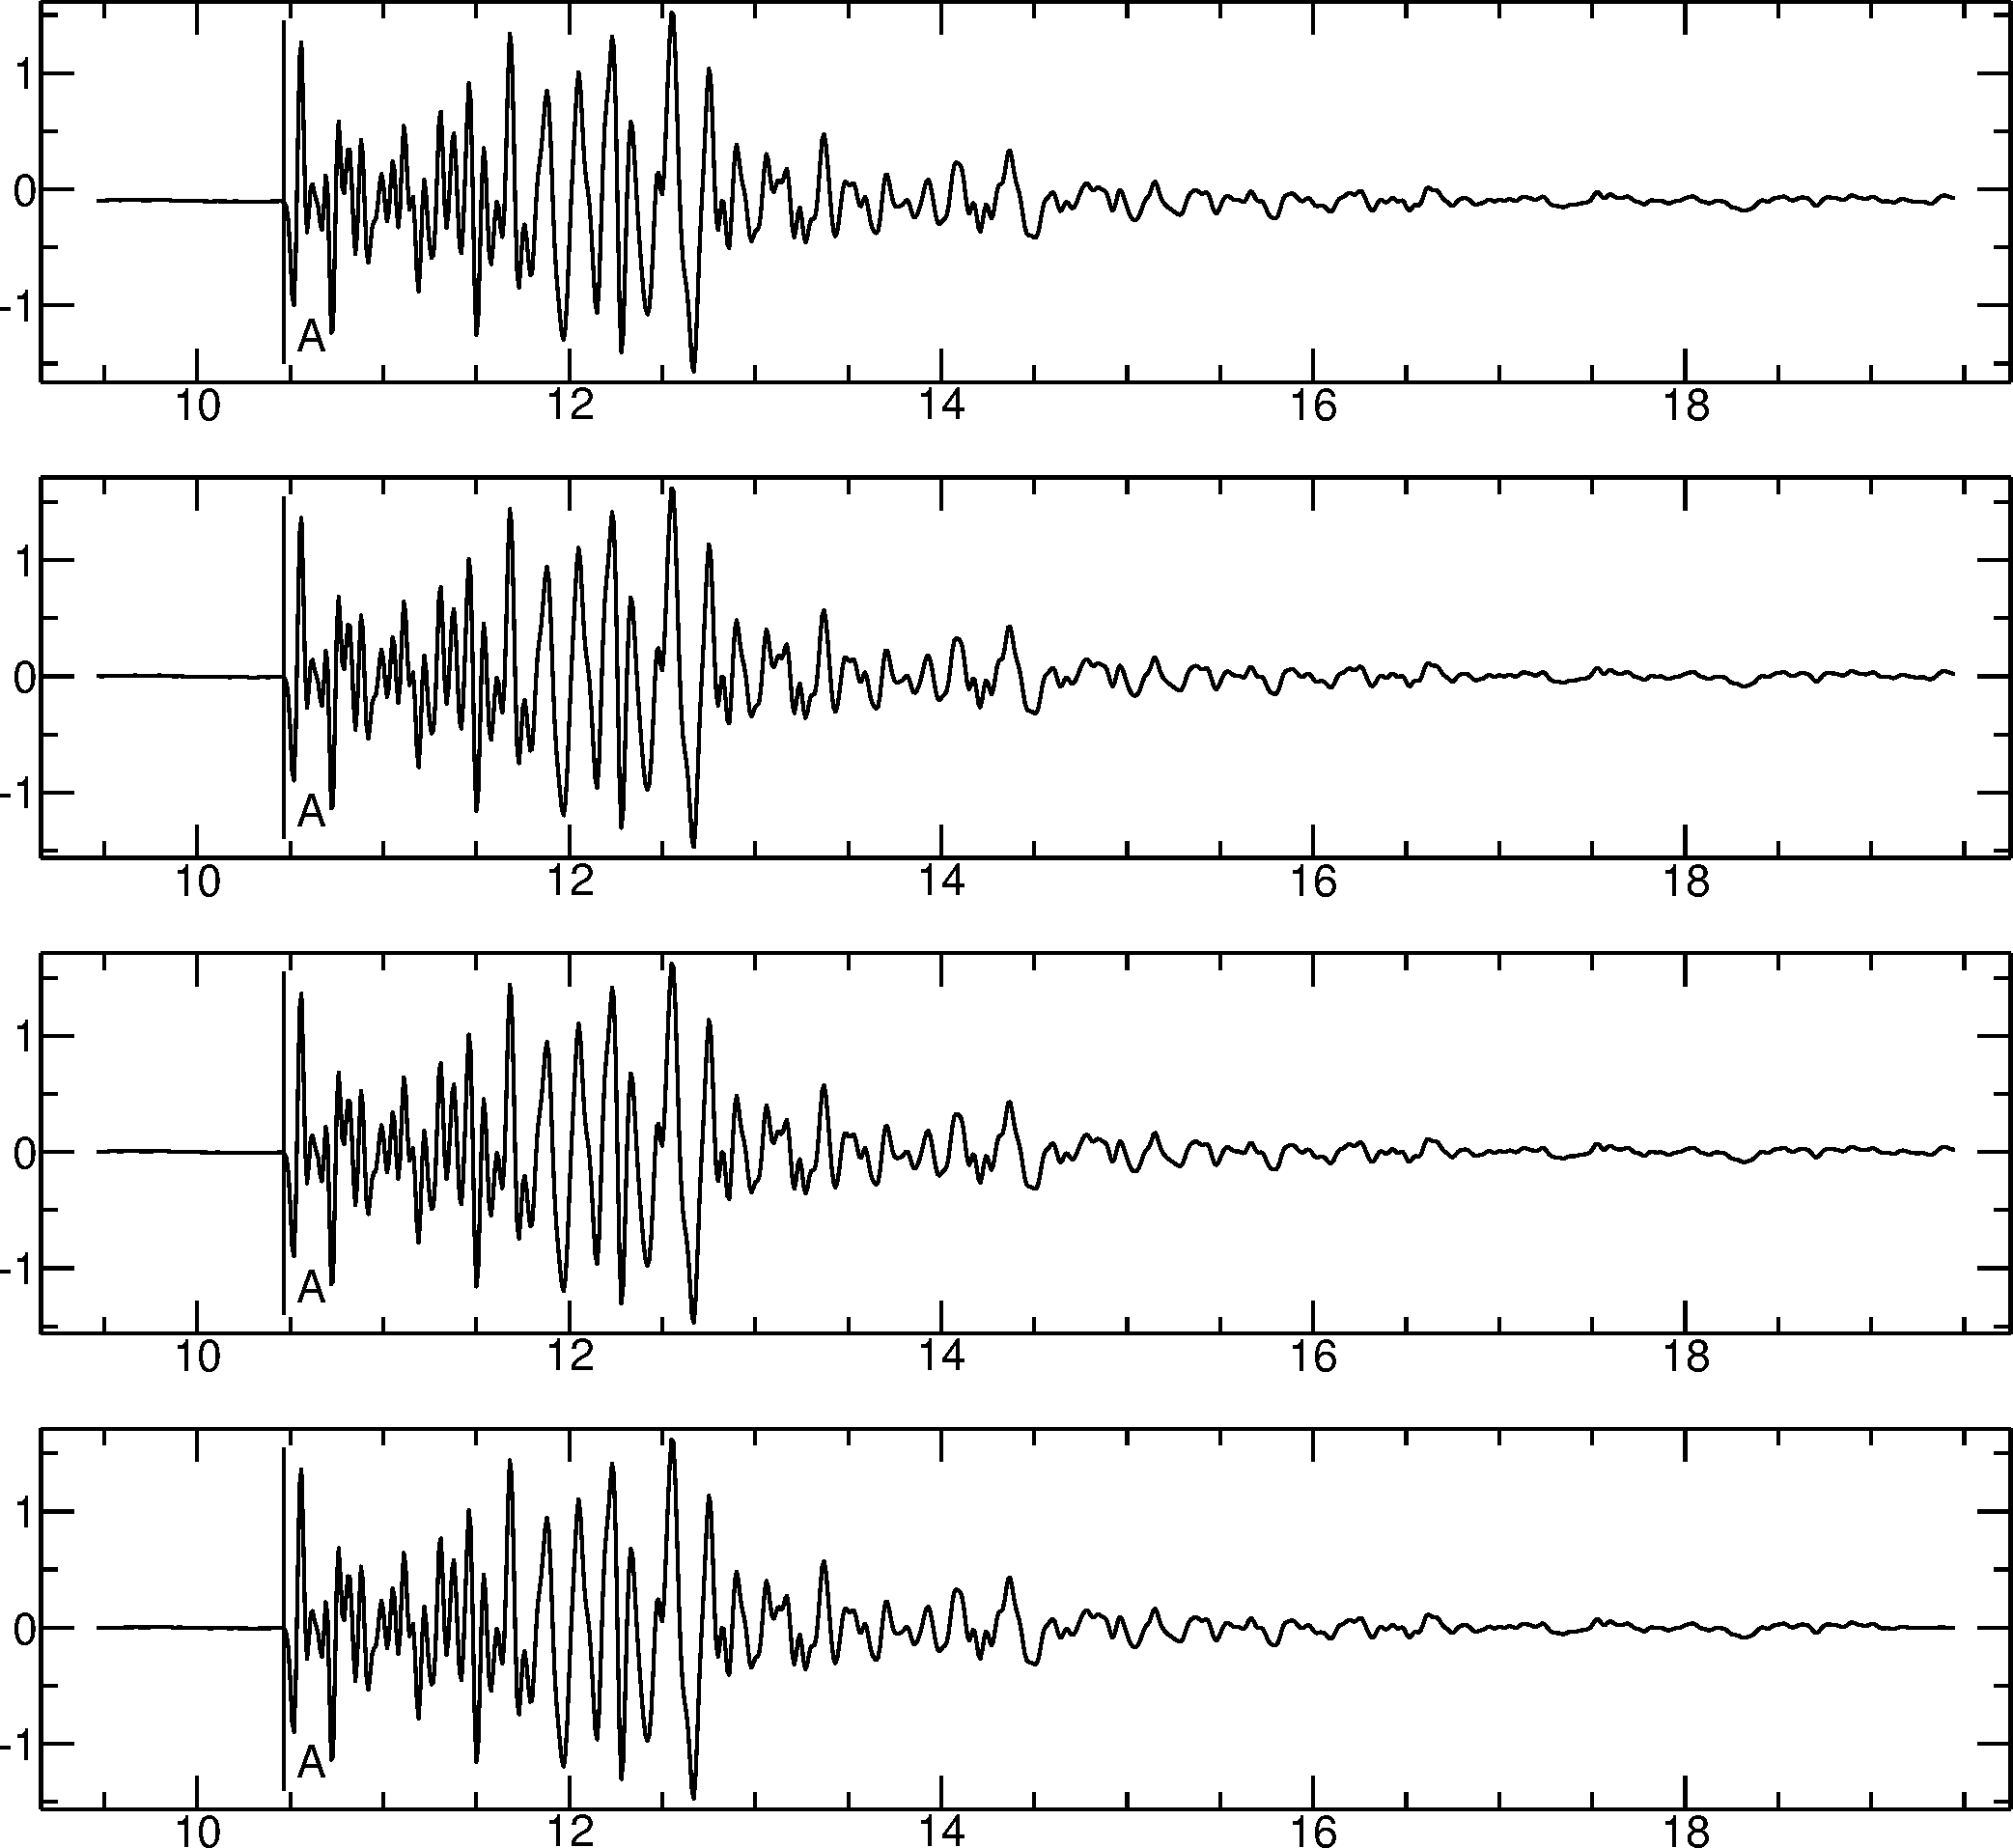
\includegraphics[width=0.9\textwidth]{rmean-rtrend-taper}
\caption{去均值、去线性趋势和波形尖灭}
\label{fig:rmean-rtrend-taper}
\end{figure}

\section{去仪器响应}
\label{sec:instrument-response}
相关命令:\nameref{cmd:transfer}

SAC中可以使用命令 \nameref{cmd:transfer} 实现去仪器响应,本节只列出日常数据处理
过程中最常用的命令。关于仪器响应的详细介绍,请参考附录``\nameref{chap:resp}''
以及教科书中的相关内容。关于 \nameref{cmd:transfer} 命令的具体用法,参考该命令的
语法说明及示例。

本节会介绍RESP文件和PZ文件的几种用法,并对每种方法的优缺点进行比较。
\subsection{RESP文件}
通常RESP文件可以通过如下命令从SEED数据中提取出来:
\begin{minted}{console}
$ rdseed -Rdf infile.seed
\end{minted}
解压得到的仪器响应文件名的格式为 \texttt{RESP.NET.STA.LOC.CHN}。

\subsubsection{RESP方法1}
\begin{SACCode}
SAC> r *.SAC
SAC> trans from evalresp to none freq 0.004 0.007 0.2 0.4
\end{SACCode}
由于波形数据和RESP文件都是用 \texttt{rdseed} 从SEED数据中解压出来的,因而二者是一一对应的。
对于内存中的每一个波形,\nameref{cmd:transfer} 命令会提取台站信息,并根据特定的格式在当前目录下
寻找对应的RESP文件。

\subsubsection{RESP方法2}
可以使用fname选项为每个波形指定RESP文件:
\begin{SACCode}
SAC> r 2006.253.14.30.24.0000.TA.N11A..LHZ.Q.SAC
SAC> rmean; rtr; taper
SAC> trans from evalresp fname RESP.TA.N11A..LHZ to none \
                                freq 0.004 0.007 0.2 0.4
\end{SACCode}

\subsubsection{RESP方法3}
把所有的PZ文件合并到同一个文件中,比如文件名叫``\texttt{RESP.ALL}'',然后使用如下命令:
\begin{SACCode}
SAC> r *.SAC
SAC> trans from evalresp fname RESP.ALL to none \
                            freq 0.004 0.007 0.2 0.4
\end{SACCode}

\subsection{PZ文件}
SAC PZ仪器响应文件可以直接用 \texttt{rdseed} 从SEED文件中提取出来:
\begin{minted}{console}
$ rdseed -pdf infile.seed
\end{minted}

\subsubsection{PZ方法1}
手动为每个波形指定PZ响应文件:
\begin{SACCode}
SAC> r OR075_LHZ.SAC
SAC> rmea; rtr; taper
SAC> trans from polezero subtype SAC_PZs_XC_OR075_LHZ to none \
                        freq 0.008 0.016 0.2 0.4
SAC> mul 1.0e9      // 用PZ文件transfer to none得到的位移数据的单位为m
                    // 而SAC默认的单位为nm,因而必须乘以1.0e9
SAC> w OR075.z      // 此时位移数据的单位为nm
\end{SACCode}

\subsubsection{PZ方法2}
可以将多个台站的PZ文件合并到一个总PZ文件中,直接使用如下命令:
\begin{SACCode}
SAC> r *.SAC
SAC> trans from pol s SAC_PZs_ALL to none freq 0.008 0.016 0.2 0.4
SAC> mul 1.0e9
SAC> w over
\end{SACCode}

\subsection{对比}
从易用性来看,RESP方法1、RESP方法3和PZ方法2都是比较易于使用的,只需要一个简单的
命令,即可对所有波形数据进行处理。而RESP方法2和PZ方法1,需要用户自己从数据文件的
文件名或头段中提取信息,并指定对应的响应文件,这需要通过写少量的脚本来实现。

从执行效率来看,做了一个简单的测试。共670个波形数据,用不同的方法去仪器响应,
完成所需时间如下:
\begin{description}
\item [RESP方法1] 58秒;
\item [RESP方法2] 43秒;
\item [RESP方法3] 227秒;
\item [PZ方法1] 8秒;
\item [PZ方法2] 90秒;
\end{description}
从中可以总结出执行效率的如下规律:
\begin{enumerate}
\item RESP2和PZ1相比,RESP3与PZ2相比,可知,PZ文件的效率要高于RESP文件。这很容易理解,
    毕竟RESP文件中包含了更为完整的信息,计算量要更大一些;PZ文件中仅包含了零极点信息
    和总增益信息,对于日常的使用来说,已经足够;
\item RESP1和RESP2相比,区别只是在于后者使用指定的文件,而后者需要自己构建文件名,
    但两者之间的执行时间却相差很多,目前无法理解这一时间差;
\item RESP3和PZ2方法,都是把多个响应函数放在同一个响应文件中,对于每个波形
    都需要对响应文件做遍历以找到匹配的响应函数,因而速度慢也是正常的;这里5倍和
    10倍的时间差还是挺大的;
\end{enumerate}

总结下来:
\begin{itemize}
\item 想要写起来简单,用RESP方法1;
\item 想要执行快,可以用PZ方法1;
\end{itemize}

\section{滤波}
相关命令:\nameref{cmd:bandpass}、\nameref{cmd:lowpass}、\nameref{cmd:highpass}、
\nameref{cmd:bandrej}

几乎所有的数据分析都需要将数据限制在一定的频率范围内,这就需要对数据做各种不同方式
的滤波。关于滤波的细节,可以参考滤波命令的相关说明,以及信号处理相关书籍。至于滤波
的范围,则依赖于具体的研究。

下图对一个脉冲波形做 \SI{0.5}{\Hz} 到 \SI{5}{\Hz} 的带通滤波,不同的滤波参数效果如下图:
\begin{figure}[H]
\centering
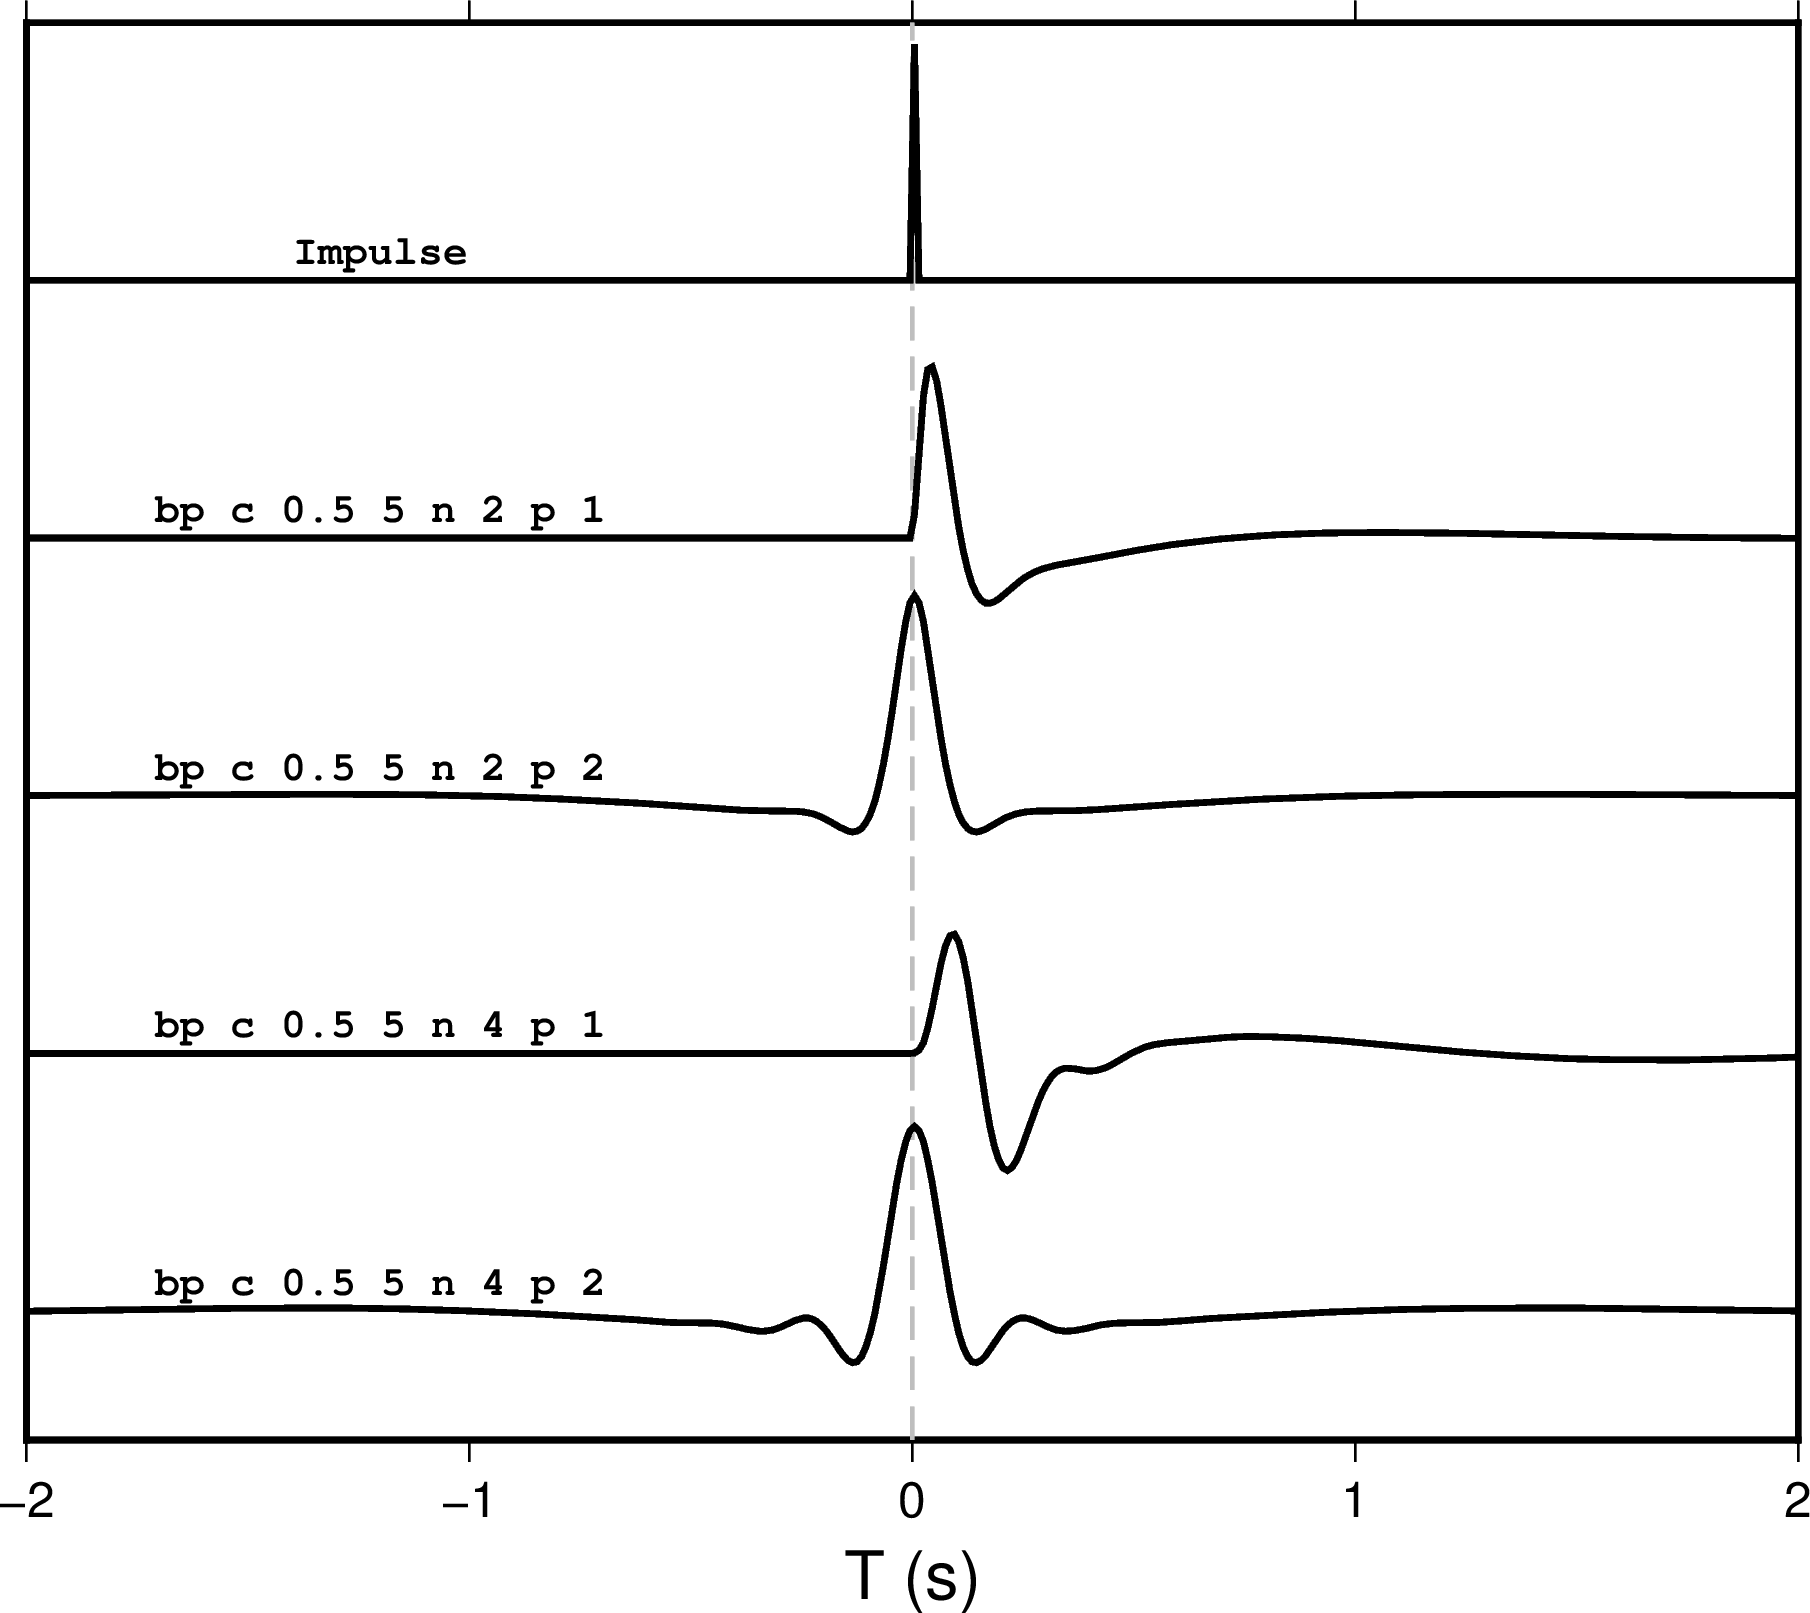
\includegraphics[width=0.8\textwidth]{filter-waveform}
\caption{不同参数的带通滤波效果}
\label{fig:filter-waveform}
\end{figure}
图 \ref{fig:filter-waveform} 中Impulse为原始脉冲波形,下面四条波形是分别取不同的n
值和p值的结果。

p取1时,对波形做一次带通滤波,由于滤波器存在相位延迟,因而导致波形的峰值出现了时间
延迟,因而会影响到震相的最大峰值的拾取,但对震相的初至却没有影响。

p取2时,对波形做正反两次带通滤波,此时不存在相位延迟,因而不会影响到最大峰值的拾取,
但震相的初至则存在时间上的提前。

\section{分量旋转}
\label{sec:traces-rotating}
相关命令:\nameref{cmd:rotate}

相关头段:\texttt{cmpinc}、\texttt{cmpaz}

三个正交的地震传感器即可完全记录地面运动矢量。因此可以将三个正交的
分量任意旋转到其它三个正交的方向上。

出于仪器安装的考虑,地震仪三分量一般都是N、E、U向的。而地震学里,
由于SH波与P-SV波的解偶,更常处理的是R、T、Z向的三分量数据。因而地震
信号的旋转是有必要的。

SAC提供了 \nameref{cmd:rotate} 命令,用于旋转任意两个水平分量。
这两个水平分量不需要正交。

\begin{SACCode}
SAC> dg sub teleseis ntkl.[enz]
/opt/sac/aux/datagen/teleseis/ntkl.e ...ntkl.n ...ntkl.z
SAC> w ntkl.e ntkl.n ntkl.z
SAC> r ./ntkl.n ./ntkl.e
SAC> lh cmpinc cmpaz
  FILE: ./ntkl.n - 1
 --------------
     cmpinc = 9.000000e+01
      cmpaz = 0.000000e+00
  FILE: ./ntkl.e - 2
 --------------
     cmpinc = 9.000000e+01
      cmpaz = 9.000000e+01
SAC> rotate to gcp              // 旋转到大圆路径
SAC> lh cmpinc cmpaz
  FILE: ./ntkl.n - 1
 --------------
     cmpinc = 9.000000e+01
      cmpaz = 2.440466e+01
  FILE: ./ntkl.e - 2
 --------------
     cmpinc = 9.000000e+01
      cmpaz = 1.144047e+02
SAC> w ntkl.r ntkl.t            // 保存为R分量和T分量
\end{SACCode}

图 \ref{fig:rotate} 中,左图中从上至下为N、E、Z分量,右图中从上至下
为R、T、Z分量。旋转到R、T分量后,可以很容易地识别出Rayleigh和Love波。

\begin{figure}[H]
\centering
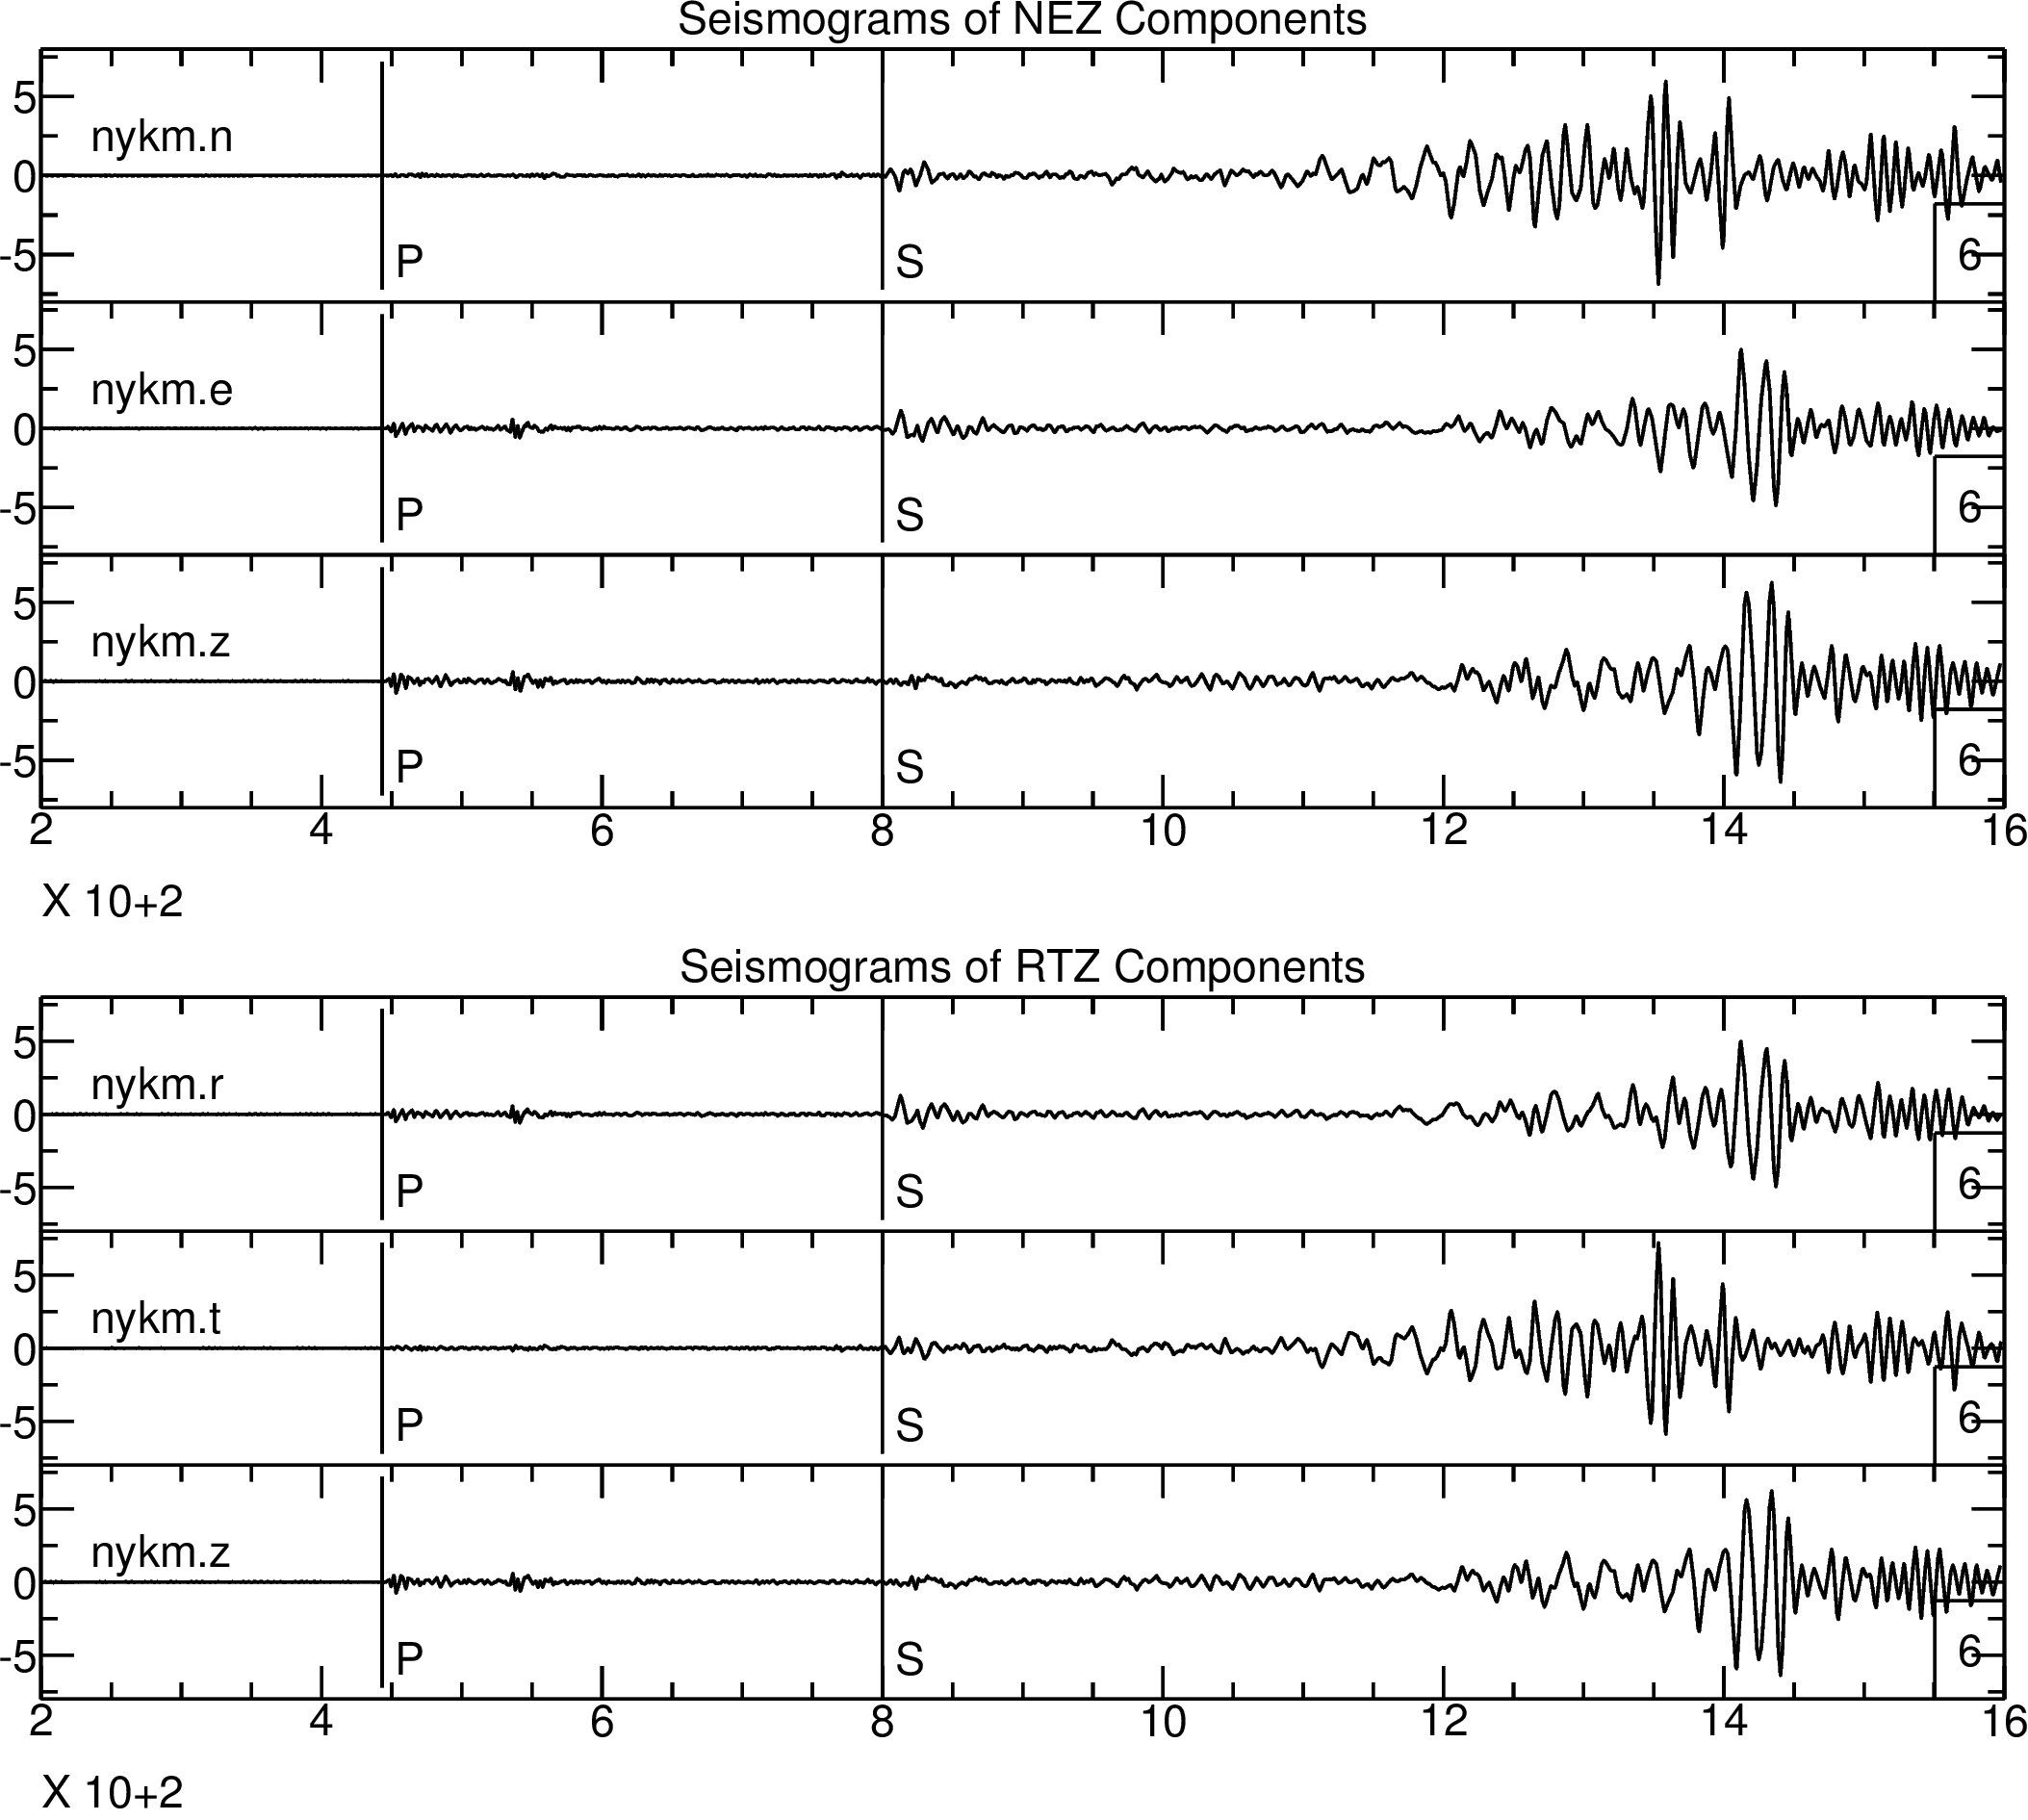
\includegraphics[width=0.95\textwidth]{rotate}
\caption[水平分量旋转]{将N、E分量旋转到R、T分量。}
\label{fig:rotate}
\end{figure}

\section{震相理论到时}
震相理论到时的计算是地震学的基础,具体的原理涉及到一大堆公式,感兴趣的读者
可以阅读相关文献。

日常工作中经常需要识别震相、将波形按理论到时排序或迭加、计算震相到时残差等等,
这些都需要用到震相理论到时。将震相理论到时写入到SAC文件的头段中,可以使得后期
处理更加简单。SAC头段中可以用于保存震相到时信息的头段包括:a、f以及tn(n=0-9),
ka、kf和ktn中则用于保存相应的震相名信息。

给SAC文件标记理论到时有三种方法,下面一一介绍。

\subsection{手动标记}
最直观的办法是根据SAC文件中的震源深度和震中距信息用某些程序计算出理论到时,
然后用 \nameref{cmd:chnhdr} 命令手动将到时信息写入到SAC头段中。
\begin{SACCode}
SAC> dg sub teleseis nykl.z     // 以nykl.z为例
SAC> lh evdp gcarc              // 查看震源深度和震中距
     evdp = 0.000000e+00
    gcarc = 3.841450e+01
// 利用某程序计算得到ak135模型下,P波走时为443.14秒,S波走时为799.05秒
// 若SAC文件的参考时间为发震时刻,则
SAC> ch t0 443.14 t1 799.05 kt0 P kt1 S
SAC> lh t0 kt0 t1 kt1
     t0 = 4.431400e+02
    kt0 = P
     t1 = 7.990500e+02
    kt1 = S
\end{SACCode}
该方法很直接也很基础, 其缺点也很明显,那就是麻烦。如果参考时刻不是发震时刻的
话,则更复杂一些。

\subsection{traveltime命令}
\nameref{cmd:traveltime} 是SAC提供的一个命令,用于计算iasp91或者ak135地球模型下
的震相理论走时,并自动将震相到时信息保存到SAC头段变量中。
\begin{SACCode}
SAC> dg sub teleseis nykl.z
SAC> traveltime model iasp91 picks 3 phase P S
traveltime: depth: 0.000000 km
SAC> lh t3 kt3 t4 kt4
         t3 = 4.430530e+02
        kt3 = P
         t4 = 7.999642e+02
        kt4 = S
\end{SACCode}
该命令会将震相P、S的理论到时依次写入头段变量t3、t4中,并在相应的K头段中写入震相名信息。
该方法的优点在于是SAC内置命令,使用起来也很简单,缺点在于只支持两种地球速度模型。

\subsection{taup\texttt{\_}setsac命令}
\verb|taup_setsac| 是taup\footnote{\url{http://www.seis.sc.edu/taup/}}软件提供的用于
计算震相理论到时的独立于SAC的外部命令。
\begin{minted}{console}
$ taup_setsac -mod prem -ph P-6,S-7 -evdpkm *.SAC
\end{minted}
该命令会根据SAC文件中的震中距和震源深度信息,计算震相在一维地球模型下的理论走时,
将震相走时写入到头段Tn中,并向KTn中写入震相名称,向USERn中写入震相的射线参数(单位
为 \si{\s\per radian})。上面的示例中,使用了PREM地球模型,将P和S的走时信息写入到头段
T6和T7中。

该方法的优点在于支持多种地球标准模型、自定义模型以及自定义震相。

\section{波形排序}
在画图时,波形数据在图像上的顺序与SAC数据读入内存时的顺序是一样的,有时候会需要对波形更加灵活的排序,比如在手动拾取震相的时候,会希望将所有波形数据按照震中距从小到大的顺序进行排列。SAC提供了 \nameref{cmd:sort} 命令使得波形可以按照某个头段变量的值进行排序。

将波形数据按照方位角升序排列:
\begin{SACCode}
SAC> r *.SAC
SAC> sort az
SAC> ppk
\end{SACCode}

将波形数据按照震中距降序排列:
\begin{SACCode}
SAC> r *.SAC
SAC> sort gcarc descend
SAC> ppk p 10
\end{SACCode}

\section{质量控制}

质量控制就是标记/删除信噪比低或不合适的波形。

用户可以自己在程序中判断数据的好坏以进行质量控制,但这样做很困难,
因为实际情况中,会遇到各种奇形怪状的``坏''波形,很难用统一的程序将
这些``坏''波形挑选出来,所以更多时候需要人工的参与。

一种常规的做法如下:
\begin{SACCode}
SAC> r *.SAC        // 读入全部的SAC数据
SAC> ppk p 5        // plotpk,每次绘制5个波形
// 若波形质量很差,则用t9标记
SAC> wh
SAC> q
\end{SACCode}

解释一下以上做法,首先读入所有的SAC数据,然后利用 \nameref{cmd:plotpk},
每次绘制n个波形,如果是3分量数据,n一般取3。若波形质量很好,则不理会;
若波形质量很差,则在波形的任意时刻标记 \texttt{t9} 的值(具体如何标记
可以参考下一节的内容),然后使用 \texttt{wh} 将标记的 \texttt{t9} 保存
到头段中,再退出SAC。

完成上面的步骤之后,所有``坏''波形的 \texttt{t9} 都被标记,一般来说都
是一个正值,而所有``好''波形的 \texttt{t9} 则都处于未定义状态,其值为
-12345.0。

鉴于此,可以通过如下命令删除``坏''波形:
\begin{minted}{console}
$ saclst t9 f *.SAC | awk '$2>0 {print "rm",$1}' | sh
\end{minted}
\begin{note}
一定要在理解该命令的含义的前提下才可使用,否则可能会造成数据的丢失!
\end{note}

当然,也可以用如下命令将``坏''数据移动到专门的目录中:
\begin{minted}{console}
$ mkdir BAD
$ saclst t9 f *.SAC | awk '$2>0 {print "mv", $1, "BAD/"}' | sh
\end{minted}
\begin{note}
awk命令中,目录名BAD后最好加上斜杠。若不加斜杠,且忘记新建目录BAD,
则所有应该放在目录BAD中的文件都会被重命名为BAD,进而导致文件丢失。
\end{note}

\section{震相拾取}%左双引号是两个倒引号,右双引号是两个单引号
\label{sec:phase-picking}
相关命令:\nameref{cmd:plotpk}

震相拾取,或者说标定到时,是SAC的一种常用功能。

要进行震相拾取,需要进入``ppk模式'':
启动SAC,读取波形数据后,在终端中键入plotpk(简写为ppk),就会出现一个绘图窗口
(如果之前没有打开绘图窗口,这个绘图窗口就成为当前窗口)。
此时,SAC就进入了ppk模式。

在介绍怎样在ppk模式中拾取震相前,先说明如何退出ppk模式,以便读者对ppk模式中命令的输入有初步认识。
要退出ppk模式,首先确保绘图窗口为当前窗口,将鼠标移入窗口中,按``q''就退出,也不需要回车。
这时,读者可以看看终端,又恢复了以前的样子。

\begin{SACCode}
SAC> fg seis
SAC> ppk        // 进入ppk模式
// 光标保持在绘图窗口上,按``q''就退出ppk模式
SAC> q          // 退出SAC
\end{SACCode}

请注意:
读者可以观察一下,ppk模式时,在终端输入任何命令,回车后,SAC返回的都是一个空行。
进入ppk模式后,在终端中键入任何命令都是无效的。
ppk模式中的命令都不在终端中输入,而是在绘图窗口中输入。

下面介绍如何在ppk模式中拾取震相:
按上面的介绍进入ppk模式,鼠标(光标)移入绘图窗口内,确定应该在何处标定到时后,移动到该处,依次按下``t''、``0'',该处即出现一条竖线,旁边有标示:``T0'',
再按下``q''以退出ppk模式。在终端键入``wh''以保存。
这样鼠标所在处的时刻即写入到头段变量t0中。SAC中供给用户标定自定义时刻的头段变量是t0到t9(详见表~\ref{table:plotpk-commands},其中有ppk模式支持的所有命令)。
注意:ppk模式的命令几乎都是由单个字符组成的,比如退出``q''(唯一的例外是命令``t'',由字符``t''和0-9的整数构成)。

\begin{SACCode}
SAC> fg seis
SAC> ppk
// 键入``t''和``0''标记到时,然后按``q''退出ppk模式
SAC> wh         // 保存头段
\end{SACCode}
以上是标定到时的基本操作。下面介绍一些保证到时标定准确的必要技巧。

首先,建议读者将移入绘图窗口内的鼠标(光标)设置成交叉瞄准线的形式。也就是像玩射击游戏时,你看到的枪炮的十字准心那样。

在``\nameref{sec:sac-install}''一节中
提到的SAC全局变量~\verb+SAC_PPK_USE_CROSSHAIRS+可以控制该光标的形态。当此全局
变量为0时,光标形态为一小十字
``\tikz[scale=0.3]{
    \draw[very thick] (0,0) -- (1,0);
    \draw[very thick] (0.5,-0.5) -- (0.5,0.5);
}'';当此全局变量为1时,会在0的基础上再加上水平和垂直线。将其值设置为1即可。
注意:改为十字准心后,要留意在输入``t''时,鼠标(光标)不仅要在窗口内,还要在波形图的图形内,否则会得到`` Bad cursor position. Please retry.''的错误提示。

其次,是图幅的放大(和缩小)。有时数据时间较长,鼠标(光标)只要移动一点就会有很大偏差,使得到时不易确定。
这时,就需要图幅的放大。首先需要将光标移动到绘图区域中的某位置,键入``x'',再移动至另一位置,
再次键入``x''。这样,两次键入就确定了一个时间窗。这时,绘图窗口中将只显示该时间窗内的波形,也就实现了图幅的放大。
可不断重复此步骤,进行多次放大。101.5之后的版本有更方便的方式:在绘图窗口中某位置按下鼠标左键,
并拖动至另一位置再松开鼠标左键,则两个位置之间的时间窗内的波形会被放大。
缩小通过``o''来实现,``o''最多可以回退5次绘图历史。

然后,就是同一台站的三个分量的数据要一次标定。同一台站的三个分量的数据上的某震相的到时自然是在同一时刻。所以把他们画一起在,就可以相互比较,利于震相的识别;
标定时一次标定,对应头段的值完全相等,这也符合到时相同的事实。
使用命令``ppk p 3 r m''进入ppk模式即可3个分量一次画图和一次标定。
进入ppk模式后,标定方式和前面类似。

\begin{SACCode}
SAC> dg sub teleseis ntkl.[nez] nykl.[nez] onkl.[nez] sdkl.[nez]
SAC> ppk p 3 r m
// 键入一次``t0''为全部波形标记到时,然后按``q''退出ppk模式
SAC> wh
SAC> q
\end{SACCode}

一般情况下,我们需要为很多台站的数据标定到时。
如果一个个台站读入,然后标定,再退出ppk模式,最后保存,就要做很多重复工作。
如果文件名已经改名为台站名开头,可以一次读入全部数据。
用命令``ppk p 3 r m''进入ppk模式,一次画三个数据。
这三个数据会恰好属于同一个台。
这个台的数据标定完以后,按``n''就可以标定下一个台。
全部标定后,再退出ppk模式,``wh''保存。

\begin{table}[H]
\centering
\small
\ttfamily
\caption{ppk模式命令一览表}
\label{table:plotpk-commands}
\begin{tabular}{cll}
	\toprule
    命令	&	含义	                                &   说明    \\
	\midrule
    a	    &	定义事件初至a                           &   1,7	    \\
    b	    &	如果有,则显示上一张绘图	            &           \\
    c	    &	计算事件的初至和结束                    &   1,4,7	\\
    d	    &	设置震相方向为DOWN	                    &           \\
    e     	&	设置震相起始为EMERGENT(急始)	        &           \\
    f	    &	定义事件结束f                           &  1,2,3,7	\\
    g	    &	以HYPO格式将拾取显示到终端              &   4   	\\
    h   	&	将拾取写成HYPO格式                      &   3,4 	\\
    i	    &	设置震相起始为IMPULSIVE	                &           \\
    j	    &	设置噪声水平                            &   2,6,8	\\
    k       &   即kill,退出ppk模式                     &           \\
    l	    &	显示光标当前位置                        &   2,4	    \\
    m	    &	计算最大振幅波形                        &   2,3,5	\\
    n	    &	显示下一绘图	                        &           \\
    o	    &	显示前一个绘图窗,最多可以保存5个绘图窗	&           \\
    p	    &	定义P波到时                             &   1,2,3,7	\\
    q	    &	即quit,退出ppk模式	                            &           \\
    s	    &	定义S波到时                             &   1,2,3,7 \\
    t	    &	用户自定义到时tn,输入t之后需要输入0到9中的任一数	&   1,2,7\\
    u	    &	设置震相方向为UP	                    &           \\
    v	    &	定义一个Wood-Anderson波形               &   2,5 	\\
    w	    &	定义一个通用波形                        &   2,5 	\\
    x	    &	使用一个新的x轴时间窗,简单说就是放大。 &           \\
    z	    &	设置参考水平                            &   2,6,8	\\
    \textbackslash	    &	删除当前全部拾取的定义。当一个文件中包含多个事件时有用。&	\\
    +	    &	设置震相方向为PLUS	                    &           \\
    -	    &	设置震相方向为MINUS	                    &           \\
    \lstinline[showspaces]! !   &	设置震相方向为NEUTRAL	                &           \\
    n	    &	设置震相质量为n,n取0-4	                &           \\
	\bottomrule
\end{tabular}
\end{table}

ppk模式经常使用的命令包括``b''、``l''、``n''、``o''、``q''、``t''和``x''。

不同的命令效果可能不同,有些会在绘图窗口显示信息,有些会将信息写入头段变量,
下面对表~\ref{table:plotpk-commands}~中的说明进行一个说明:
\begin{description}
    \item [1] 会将信息写入头段变量
    \item [2] 写入字符型震相拾取文件(若已打开)
    \item [3] 写入HYPO格式震相拾取文件(若已打开)
    \item [4] 在绘图窗口中显示信息
    \item [5] 窗口显示包含波形的矩形
    \item [6] 在指定的水平处放置水平光标
    \item [7] 绘图窗口显示含有到时标识的垂直线
    \item [8] 绘图窗口显示含有标识的水平线
\end{description}

\section{数据截窗}
相关命令:\nameref{cmd:cut}

数据申请时一般会选择尽可能长的时间窗,而实际进行数据处理和分析时可能只需要其中
的一小段时间窗,这就需要对数据时间窗进行截取。

SAC中的 \nameref{cmd:cut} 命令可以实现数据截取,需要注意的是,该命令时
``参数设定类'' 命令,即需要先执行cut命令再执行read命令。

\subsection{pdw}
\label{subsec:pdw}
使用cut命令对数据进行截取时需要定义数据时间窗。除了截取数据之外,其他一些命令
也会需要定义时间窗,比如 \nameref{cmd:rms}、\nameref{cmd:mtw}、\nameref{cmd:xlim} 等,
这些命令都使用同样的方式定义时间窗,在SAC中称为pdw,即partial data window。

pdw定义了一个开始时间和一个结束时间,其格式为 \texttt{ref offset ref offset}。
其中ref为参考时刻,可以取Z、B、E、O、A、F、N和Tn(n=0--9),而offset为相对于参考时刻的时间偏移量。

参考时刻ref可以取如下值:
\begin{itemize}
\item B:磁盘文件起始值
\item E:磁盘文件结束值
\item O:事件开始时间
\item A:初动到时
\item F:信号结束时间
\item Tn:用户自定义时间标记,n = 0--9
\item Z:参考时刻
\item N:将offset解释为数据点数而非时间偏移量,其仅可以用于结束值
\end{itemize}

若开始或结束的offset省略则认为其值为0。若开始ref省略则认为其为Z;若结束ref省略则
认为其值与开始ref相同。

下面的例子中展示了一些常见的pdw及其含义:
\begin{SACCode}
 B E            // 文件开始到文件结束,即与cut off相同
 B 0 30         // 文件开始的30秒
 A -10 30       // 初动前10秒到初动后30秒
 B N 2048       // 文件最初的2048个点
 T0 -10 N 1000  // 从T0前10秒起的1000个点
 30.2 48        // 相对磁盘文件0点的30.2到48秒
\end{SACCode}

\subsection{cut}
\nameref{cmd:cut} 命令是``参数设定类''命令,因而需要先cut再read:
\begin{SACCode}
SAC> cut t0 -5 5        // 截取t0前后各5秒,共计10秒的数据
SAC> r *.SAC            // 先cut再read
\end{SACCode}

\section{数据分析}
数据分析是整个科学研究的核心。SAC软件只是负责完成前期的预处理工作,
真正核心的数据分析工作通常需要用户自己写程序完成。
但无论怎样都牵涉到如何在程序中读写SAC文件的问题,这个问题放在
``\nameref{chap:sac-libs}''和``\nameref{chap:sac-io}''
这两章中具体说明。


\chapter{SAC图像}
\label{chap:sac-graphics}
\section{图形设备}
SAC支持两种图形设备,分别是xwindows和sgf,默认的图形设备是xwindows。可以使用
\nameref{cmd:begindevices} 和 \nameref{cmd:enddevices} 命令开启/关闭指定的图形设备;
同时也可以使用 \nameref{cmd:setdevice} 命令设定默认的图形设备。

\subsection{xwindows}
xwindows即X Window System,也称为X11或X,是一种以位图方式显示的软件窗口系统。
几乎所有的现代操作系统都能支持与使用X,Linux下知名的桌面环境GNOME和KDE也都是以
X窗口系统为基础建构成的。

\begin{figure}[H]
\centering
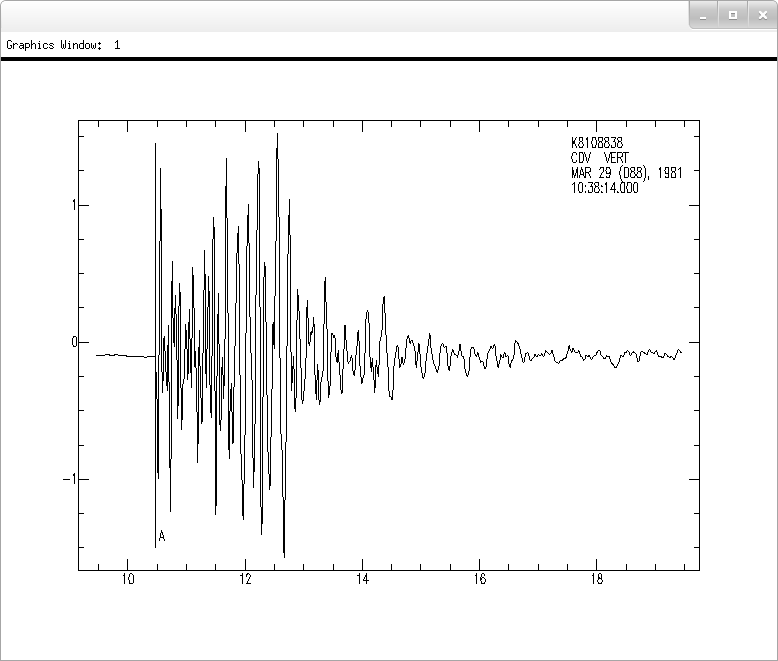
\includegraphics[width=0.9\textwidth]{window}
\caption{SAC绘图窗口}
\label{fig:plot}
\end{figure}

图 \ref{fig:plot} 展示了SAC中的xwindows图形设备的外观,它是SAC默认的图形设备。
同很多其它软件界面类似,xwindows窗口在左上角显示图标,右上角显示``最小化''、
``最大化''、``还原''和``关闭''按钮。窗口的中间部分为真正的绘图区,
本文档的其余插图将只给出绘图区的图像而不再包含窗口部分。

左上角的``Graphics Window: 1''指明了当前绘图窗口的编号为``1'',
SAC最多支持同时打开10个X窗口,编号为1--10。默认情况下只启动并使用1号X窗口。
\nameref{cmd:beginwindow} 命令用于启动指定编号的X窗口;
\nameref{cmd:window} 命令还可以设置每个X窗口的长宽比以及X窗口相对于屏幕的位置。

\subsection{sgf}
SGF,全称SAC Graphic File,即SAC图形文件,是SAC自定义的一种文件格式,其包含了
绘制一个图件所需要的全部信息,可以通过 \nameref{sec:sgftops} 等工具转换到
其它图形设备或图形文件格式。

若启用了SGF图形设备,每次绘制的图件将分别保存到单独的sgf文件中。默认情况下,sgf图形文件的
文件名格式为 \texttt{fnnn.sgf} ,其中``nnn''为图件编号,起始编号为001,
每生成一个图件该编号递增。
\nameref{cmd:sgf} 命令可以控制SGF图形设备的选项,比如文件名前缀(默认为 \texttt{f})、
起始编号(默认从 \texttt{001} 开始)、保存目录、文件尺寸等。

\section{SAC绘图流程}
严格地说,SAC绘图的流程应该是:启动图像设备$\rightarrow$绘图$\rightarrow$关闭图像设备。
如下所示:
\begin{SACCode}
SAC> r cdv.[nez]
SAC> begindevices xwindows      // 启动图像设备xwindows,简写为bd x
SAC> p                          // 绘图
Waiting
Waiting
SAC> enddevices xwindows        // 关闭图像设备xwindows,简写为ed x
SAC> q
\end{SACCode}

上面的步骤稍显繁琐,SAC将这一流程进行了简化。在第一次执行绘图命令前,
SAC偷偷启动了默认的图像设备xwindows,接下来的绘图工作都在该窗口中完成。
当用户退出SAC时,SAC会自动关闭图像设备。

也许你已经发现,即使plot结束或者中途退出plot,绘图窗口依然没有被关闭。
即便点击窗口的``关闭''按钮,窗口依然无法关闭。若想要关闭绘图窗口,应
如上例那样使用 \texttt{ed x} 命令。

\section{绘图命令}
SAC提供了许多与绘图有关的命令,包括控制图像外观的参数控制类命令以及执行绘图功能
的操作执行类命令。这一节将介绍常用的几个操作执行类命令。

\subsection{plot}
\nameref{cmd:plot} 命令会绘制内存块中的所有波形数据,但每次只显示一个波形,然后等待用户输入
再决定是否显示下一个波形。该命令的具体用法在第 \ref{sec:display} 节已经详细介绍。

\subsection{plot1}
\nameref{cmd:plot1} 命令会绘制内存块中的所有波形数据,在一个窗口中一次显示多个波形,
这些波形共用一个X轴(时间轴),但拥有单独的Y轴。

\begin{SACCode}
SAC> dg sub local cdv.[enz]
cdv.e cdv.n cdv.z
SAC> p1
\end{SACCode}

执行 \nameref{cmd:plot1} 命令后,焦点位于图形窗口,显示如图 \ref{fig:plot1}。
\begin{figure}[H]
\centering
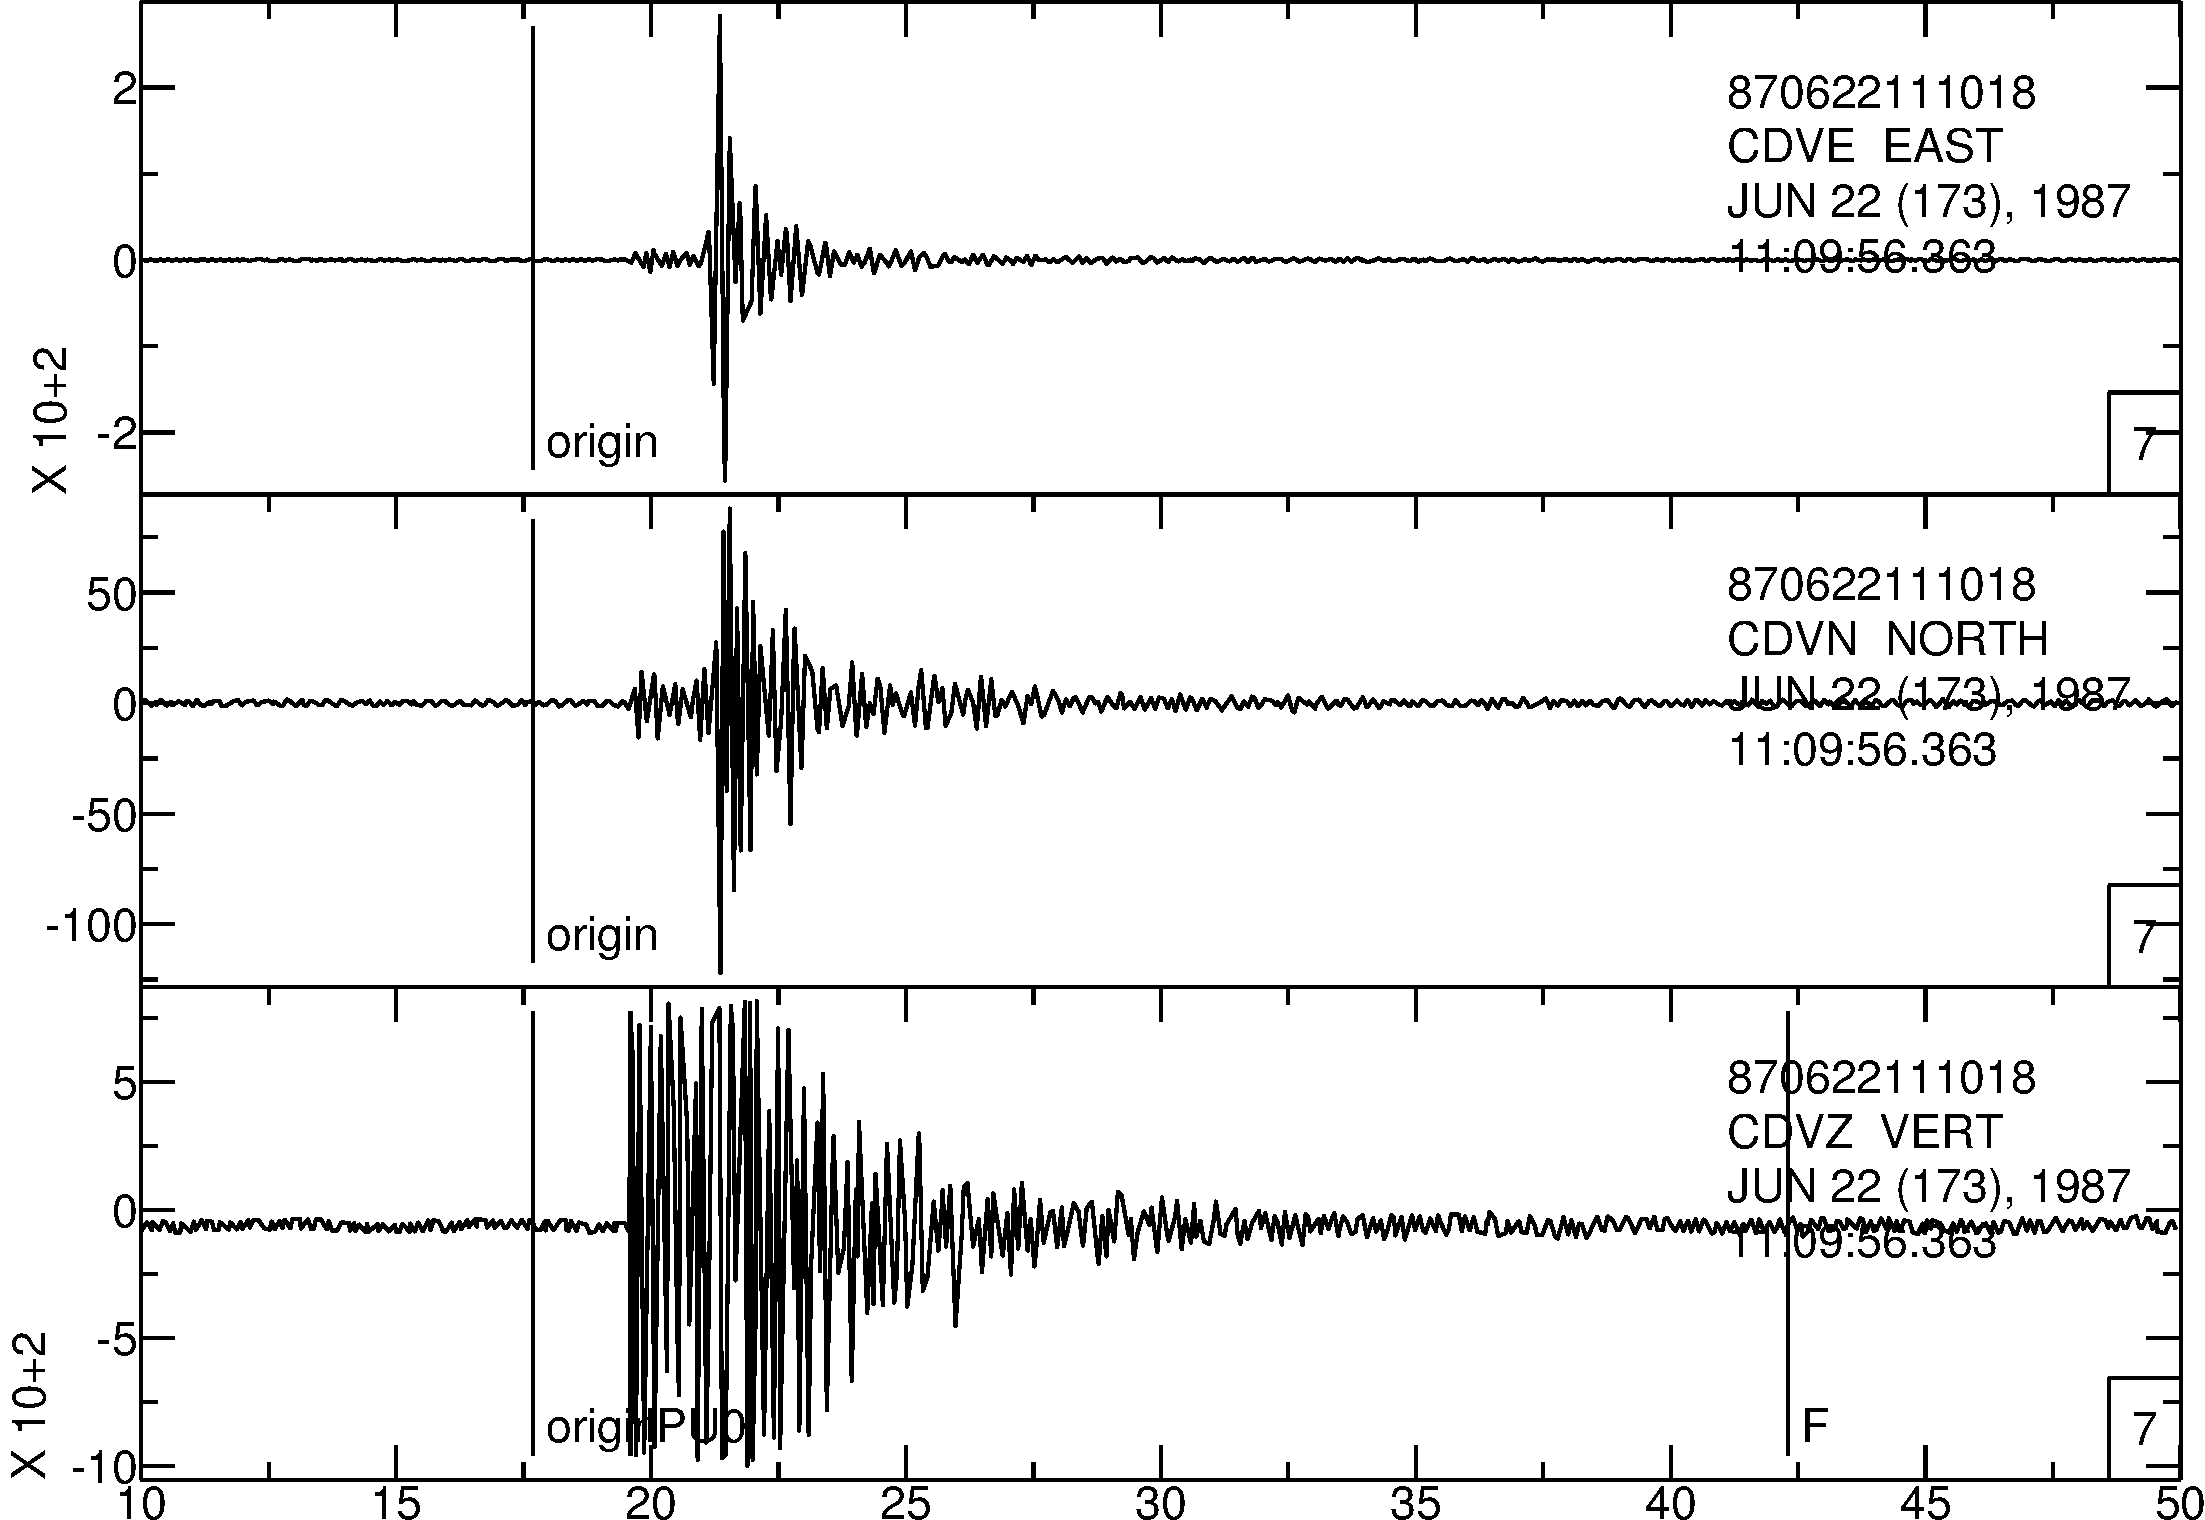
\includegraphics[width=0.85\textwidth]{plot1}
\caption{plot1绘图效果}
\label{fig:plot1}
\end{figure}

当一次性读入多个波形数据时,若直接使用 \nameref{cmd:plot1} 绘图,会一次性显示全部波形,导致
窗口内波形太密,反而什么都看不清。\nameref{cmd:plot1} 提供了``\texttt{perplot n}''选项以
指定窗口内一次最多显示多少个波形,余下的波形则处于等待状态。在查看波形的时候,
经常需要将每个台站的三分量波形记录放在一起看,此时设置选项 \texttt{perplot} 的参数值为 \texttt{3} 即可。
\begin{SACCode}
SAC> dg sub local cdv.[enz] cvl.[enz] cvy.[enz]  // 生成9个地震波形
cdv.e cdv.n cdv.z cvl.e cvl.n cvl.z cvy.e cvy.n cvy.z
SAC> p1 p 3         // p是选项perplot的简写,3代表每次显示3个波形
Waiting
Waiting
SAC>
\end{SACCode}

默认情况下,所有的波形数据会按照绝对时间(\texttt{absolute})对齐,若波形数据
具有不同的开始时间,则波形数据之间会出现相对错动;也可以使所有的波形数据相对于
(\texttt{relative})各自的开始时间绘图,此时X轴的起始坐标为0。

\subsection{plot2}
\nameref{cmd:plot2} 会一次性将内存块中的所有波形绘制在一个窗口内,所有的波形共用X轴,因而绘图
时也可以使用绝对模式或相对模式。与 \nameref{cmd:plot1} 不同的是,所有的波形还同时共用Y轴,因而
波形会相互覆盖。

\nameref{cmd:plot2} 适合绘制多个波形的对比图,常用于数据处理前后波形对比或真实波形与合成波形间的对比。
\begin{SACCode}
SAC> fg seis                     // 生成数据
SAC> rmean; rtrend; taper        // 预处理
SAC> w seis.0                    // 写入滤波前文件
SAC> bp c 0.05 10 n 4 p 2        // 滤波
SAC> w seis.1                    // 写入滤波后文件
SAC> r ./seis.[01]               // 读入两个文件
./seis.0 ...seis.1
SAC> color red inc list red blue // 对两个数据分别设置红色和蓝色
SAC> p2                          // 绘图
\end{SACCode}
图 \ref{fig:plot2} 中红线为滤波前波形,蓝线为滤波后波形,二者共用X轴和Y轴,
从这样的波形对比图中,可以很明显得看到滤波对于波形的影响。

\begin{figure}[H]
\centering
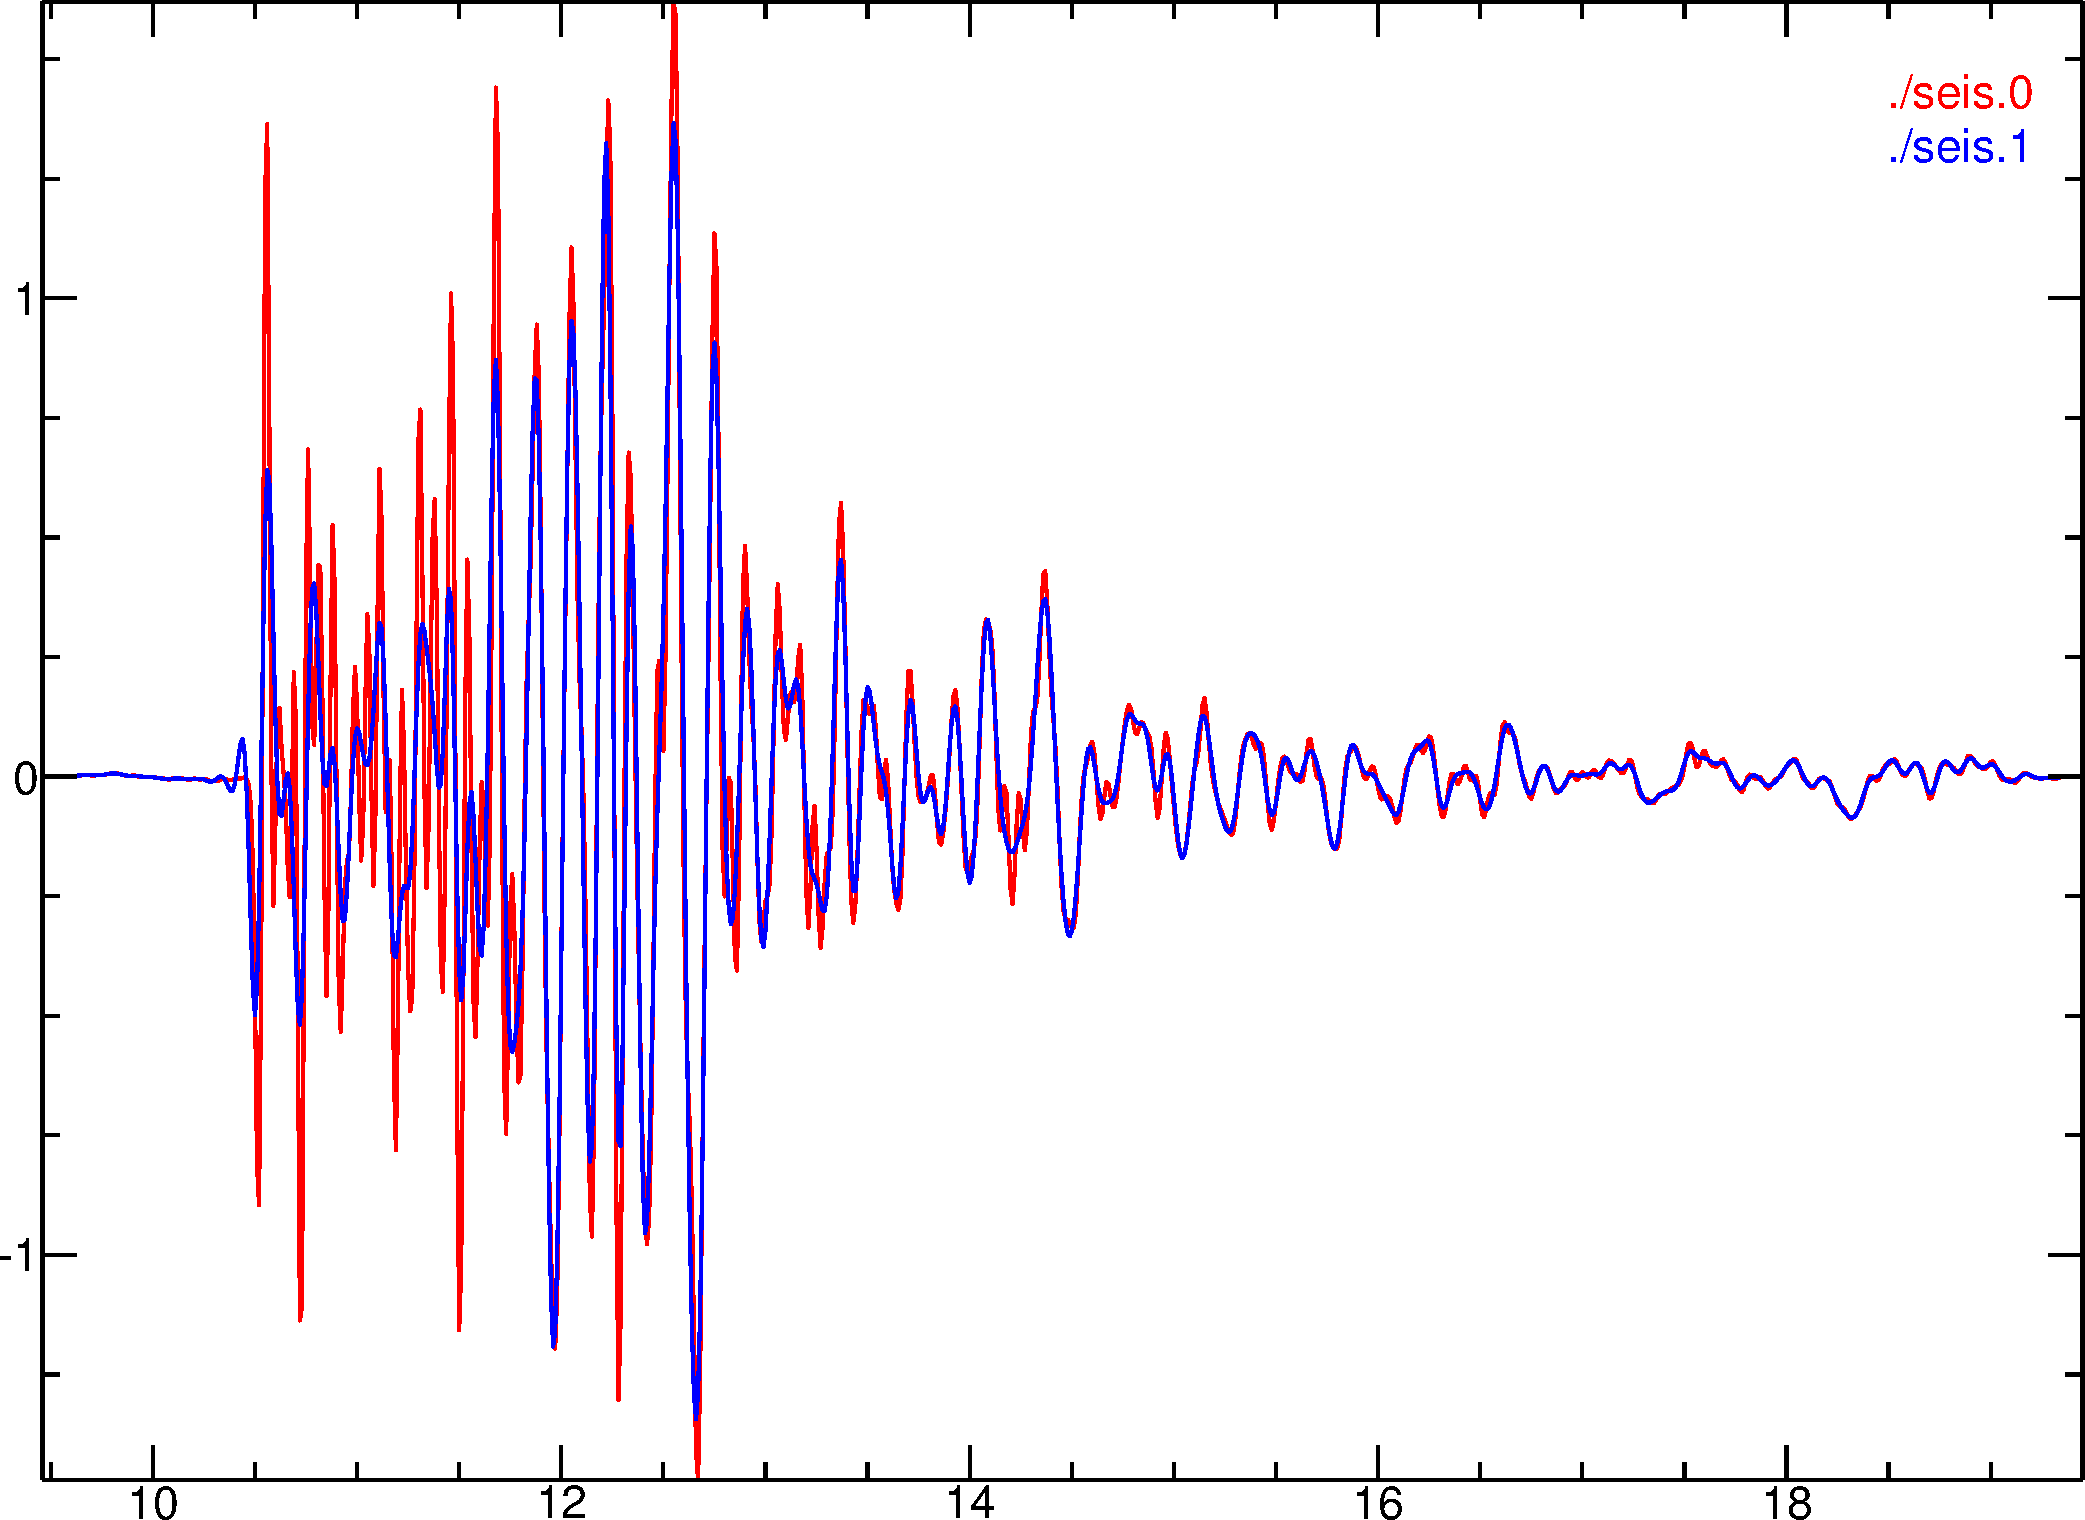
\includegraphics[width=0.85\textwidth]{plot2}
\caption[plot2绘图效果]{plot2绘图效果。红色为滤波前波形,蓝色为滤波后波形。}
\label{fig:plot2}
\end{figure}

\subsection{plotpk}
\nameref{cmd:plotpk} 是SAC中最常用的命令之一。其可以在窗口中显示指定个数的波形,所有波形共用X轴,
但拥有单独的Y轴。该命令主要用于震相拾取,在``\nameref{sec:phase-picking}''一节
有详细介绍。

\subsection{plotpm}
\nameref{cmd:plotpm} 可以利用成对的波形数据,提取出任一时间段内两个波形数据的振幅信息,绘制在
``振幅-振幅''图中。若一对波形数据恰好是同一台站两个互相垂直的分量,
则``振幅-振幅''图即为``质点运动图''。从``质点运动图''中,可以提取出震相的一些重要信息。

下面的例子利用垂直和径向分量的波形数据绘制Rayleigh面波的质点运动轨迹:
\begin{SACCode}
SAC> dg sub tele nykl.z             // Z分量
SAC> w nykl.z
SAC> dg sub tele nykl.e nykl.n      // E、N分量
SAC> rotate to gcp                  // 旋转至大圆路径
SAC> w nykl.r nykl.t                // R、T分量
SAC> r nykl.z nykl.r                // 读入Z和R分量
SAC> xlabel 'Radial component'
SAC> ylabel 'Vertical component'
SAC> title 'Particle-motion plot for partial Rayleigh wave'
SAC> xlim 1300 1340                 // 仅绘制Rayleigh面波的部分时间窗
SAC> ppm                            // 绘制质点运动图
\end{SACCode}

鉴于 \nameref{cmd:plotpm} 命令绘图的效果很糟糕,就不再贴效果图了,读者可以根据上面的命令自行绘制。

\subsection{plotsp}
\nameref{cmd:plotsp} 命令用于绘制不同格式的谱文件,可以绘制``振幅+相位''或者``实部+虚部'',
同时可以任意指定X、Y轴为线性轴或对数轴。

下面的命令对波形数据进行FFT得到谱文件,并使用 \nameref{cmd:plotsp} 命令绘制其振幅谱:
\begin{SACCode}
SAC> fg seis
SAC> fft
SAC> psp am loglog
\end{SACCode}

\begin{figure}[H]
\centering
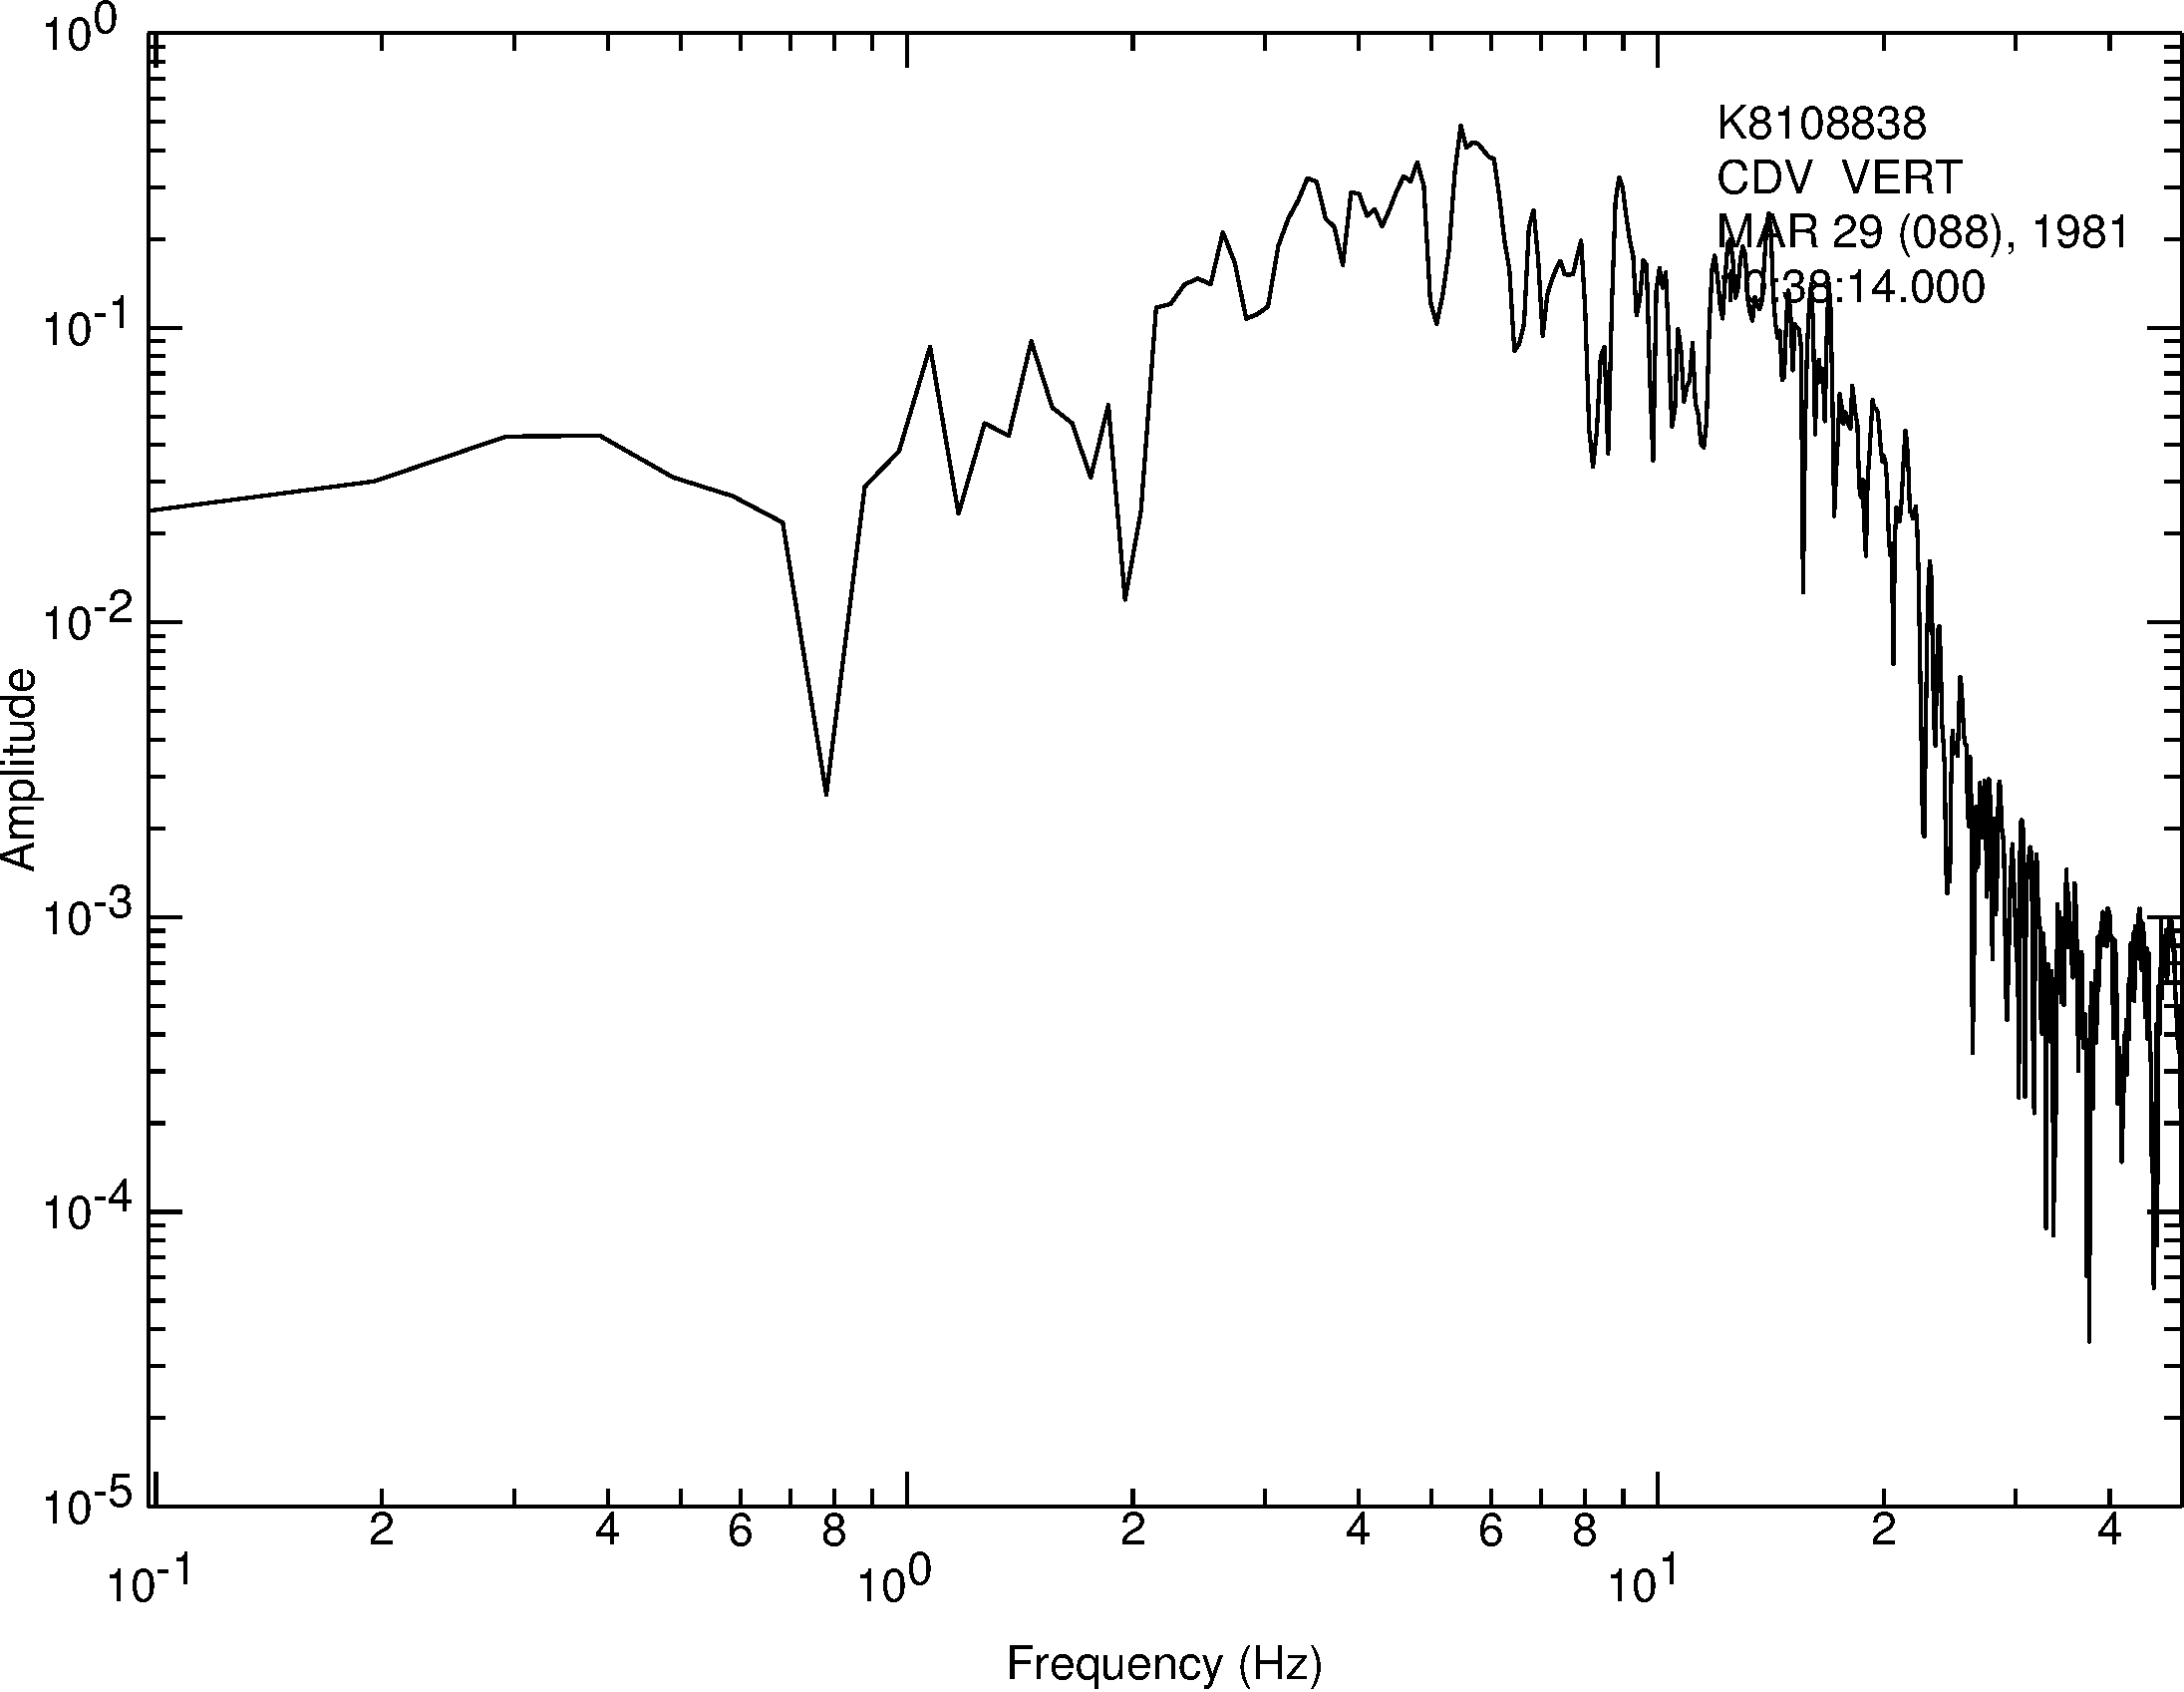
\includegraphics[width=0.95\textwidth]{plotsp}
\caption{plotsp绘制振幅谱}
\label{fig:plotsp}
\end{figure}
\section{图像外观}
\label{sec:plot-appearance}

\subsection{图像元素}
对于SAC而言,最基本的显示元素是将所有数据点用线连起来所构成的地震图。除此之外,
SAC的绘图命令还会在图像的四个边绘制坐标轴以及刻度,为图像添加标题、轴标签等。

图 \ref{fig:plot-appearance} 展示了一个完整的SAC图像所包含的所有元素。

\begin{figure}[H]
\centering
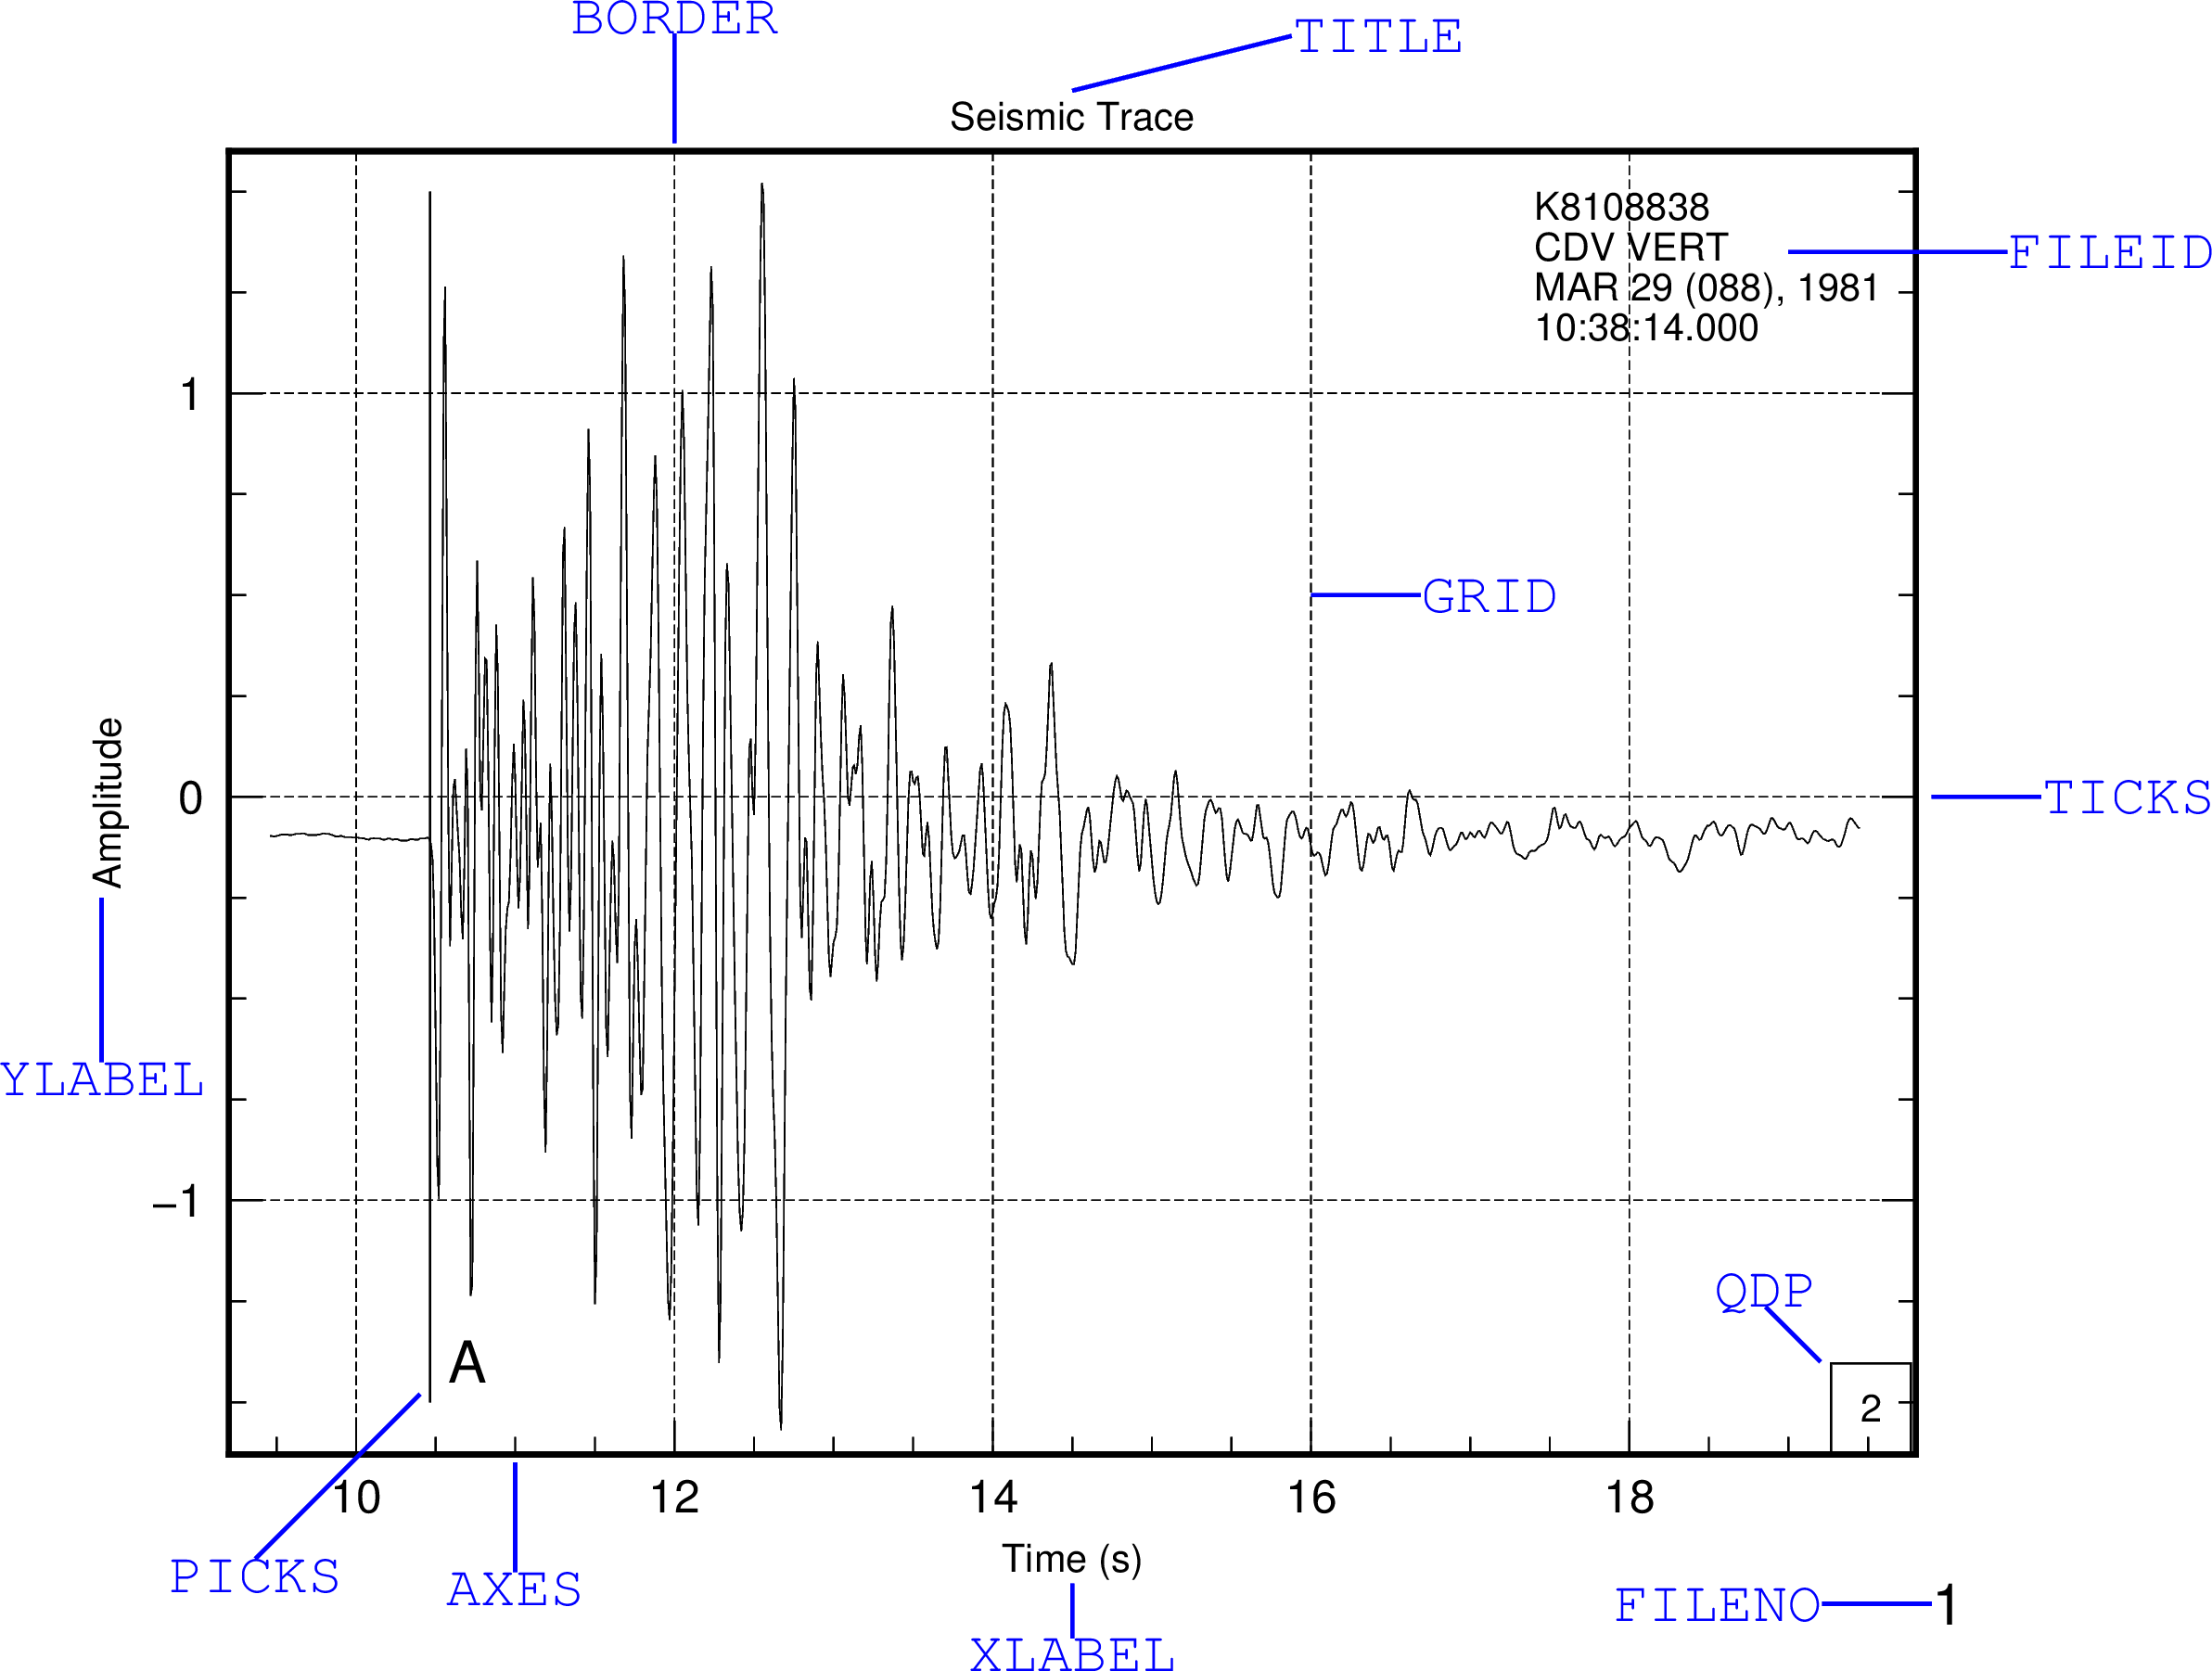
\includegraphics[width=0.9\textwidth]{appearance}
\caption[绘图外观相关命令]{绘图外观及其相关命令。图中蓝色部分为对绘图外观的说明。}
\label{fig:plot-appearance}
\end{figure}

图 \ref{fig:plot-appearance} 可以用如下命令绘制得到:
\begin{SACCode}
SAC> fg seis                // 生成数据
SAC> qdp on                 // 打开QDP选项(默认值即为开)
SAC> grid on                // 显示网格
SAC> title 'Seismic Trace'  // 设置标题
SAC> xlabel "Time(s)"       // 设置x轴标签
SAC> ylabel "Amplitude"     // 设置y轴标签
SAC> filenumber on          // 显示文件号
SAC> axes only left bottom  // left和bottom显示axes
SAC> ticks only right       // right显示ticks
SAC> border on              // top显示border
SAC> p                      // 绘图
\end{SACCode}

图像中显示的元素包括:
\subsubsection{标签}
标签大致可以分为三种:标题、轴标签和通用标签。
\begin{description}
\item[TITLE] 图像的标题。\nameref{cmd:title} 命令可控制标题文本、位置和尺寸
\item[XLABEL、YLABEL] 轴标签。\nameref{cmd:xlabel} 和 \nameref{cmd:ylabel} 命令可
    指定X和Y轴标签文本、位置和尺寸。
\item[PLABEL] 通用标签。\nameref{cmd:plabel} 可指定通用标签的文本、位置和尺寸。
\end{description}

标签文本需要用单引号或双引号包围,文本尺寸SIZE可以选择TINY、SMALL、MEDIUM或LARGE,
文本位置LOCATION则可以取TOP、BOTTOM、LEFT或RIGHT。

可以通过 \nameref{cmd:plabel} 命令定义最多三个通用标签。通用标签与轴标签类似,其
更通用之处在于可以任意指定其位置。每个标签可以用 \texttt{POSITION x y a} 来指定
其位置,其中x、y为标签位置相对于窗口尺寸的比例,a表示标签相对于水平方向顺时针旋转
的角度;也可以用 \texttt{BELOW} 设置新标签位于上一标签的下方。

\subsubsection{标记}
图像中包含了如下标记:
\begin{description}
\item [FILEID] 文件ID。\nameref{cmd:fileid} 用于控制文件ID的内容、位置及其格式。
\item [FILENO] 文件号。\nameref{cmd:filenumber} 控制文件号显示与否。
\item [PICKS] 到时标记。\nameref{cmd:picks} 用于控制是否显示到时标记以及显示效果。
\item [QDP] QDP因子。\nameref{cmd:qdp} 用于控制qdp因子的大小。
\end{description}

QDP,全称为``quick and dirty plot''。在开发SAC的那个年代,计算机的性能一般,
若在绘图时绘制全部数据点,则绘图过程会耗费大量时间。因而SAC采用了``qdp''的方式:
每隔若干个数据点绘制一个数据点\footnote{本质上就是绘图时的一次``减采样'',但是没有做抗混淆处理。}。
图中右下角的``2''即表示每两个点中绘制一个点。
目前计算机的性能已经足够强大,因而一般使用 \texttt{qdp off} 命令关于该选项。

\subsubsection{框架}
每张图都有一个框架,每个框架有TOP、BOTTOM、LEFT和RIGHT四条边。

SAC中,每条边都可以用四种不同的形式表示:
\begin{itemize}
\item 不绘制;
\item border:仅一条直线,即图 \ref{fig:plot-appearance} 中TOP边;
\item ticks:直线+刻度\footnote{刻度专指每条边上的短线。},即图中RIGHT边;
\item axes:直线+刻度+标注\footnote{标注专指每条边上的数字。},即图中LEFT边和BOTTOM边;
\end{itemize}

从上面的定义可以看到,四种形式的边存在包含与被包含的关系,因而在设定边时,有如下规则:
\begin{enumerate}
\item 用 \nameref{cmd:axes} 控制在哪些边使用``axes'';
\item 只有不使用``axes''的边才可以用 \nameref{cmd:ticks} 命令控制是否使用``ticks'';
\item 只有不使用``axes''和``ticks''的边才可以使用 \nameref{cmd:border} 命令控制是否使用``border'';
\item 不使用``axes''、``ticks''和``borders''的边则不绘制。
\end{enumerate}

除了边之外,还可以使用 \nameref{cmd:grid} 命令控制网格的显示以及网格的线型,或使用
\nameref{cmd:xgrid}、\nameref{cmd:ygrid} 分别控制横、纵方向网格的显示和属性。

\subsection{图像控制}
\subsubsection{坐标轴}
SAC使用了优秀的默认算法,根据要绘制的数据范围选择合适的刻度间隔和标注。若对于默认
的结果不满意,可以使用SAC提供的命令分别对X、Y坐标轴进行调整,下面仅列出与X轴相关的
命令。
\begin{description}
\item [xlim] 控制绘图的X轴范围
\item [xdiv] 控制X轴刻度间隔
\item [xfudge] 设定fudge因子,根据数据极值扩展X轴范围
\end{description}

\subsubsection{坐标系}
绘制时间序列一般使用线性坐标系,SAC也提供了一系列命令以指定X、Y轴为线性坐标轴或
对数坐标轴。这些命令包括: \nameref{cmd:linlin}、\nameref{cmd:linlog}、\nameref{cmd:loglin}、
\nameref{cmd:loglog}、\nameref{cmd:xlin}、\nameref{cmd:xlog}、\nameref{cmd:ylin}、
\nameref{cmd:ylog}。

对于对数坐标轴,还有一些命令可以控制其外观,比如 \nameref{cmd:xfull}、\nameref{cmd:loglab}、
\nameref{cmd:floor}。

\subsection{线条属性}
\label{subsec:line-attribution}

线条的属性包括线型(\nameref{cmd:line})、线宽(\nameref{cmd:width})、
颜色(\nameref{cmd:color})和符号(\nameref{cmd:symbol})。

下面的命令展示了如何修改线条的属性。
\begin{SACCode}
SAC> fg seis
SAC> line 3         // 线型为3
SAC> width 2        // 线宽为2
SAC> color red      // 红色
SAC> p
\end{SACCode}

\begin{figure}[H]
\centering
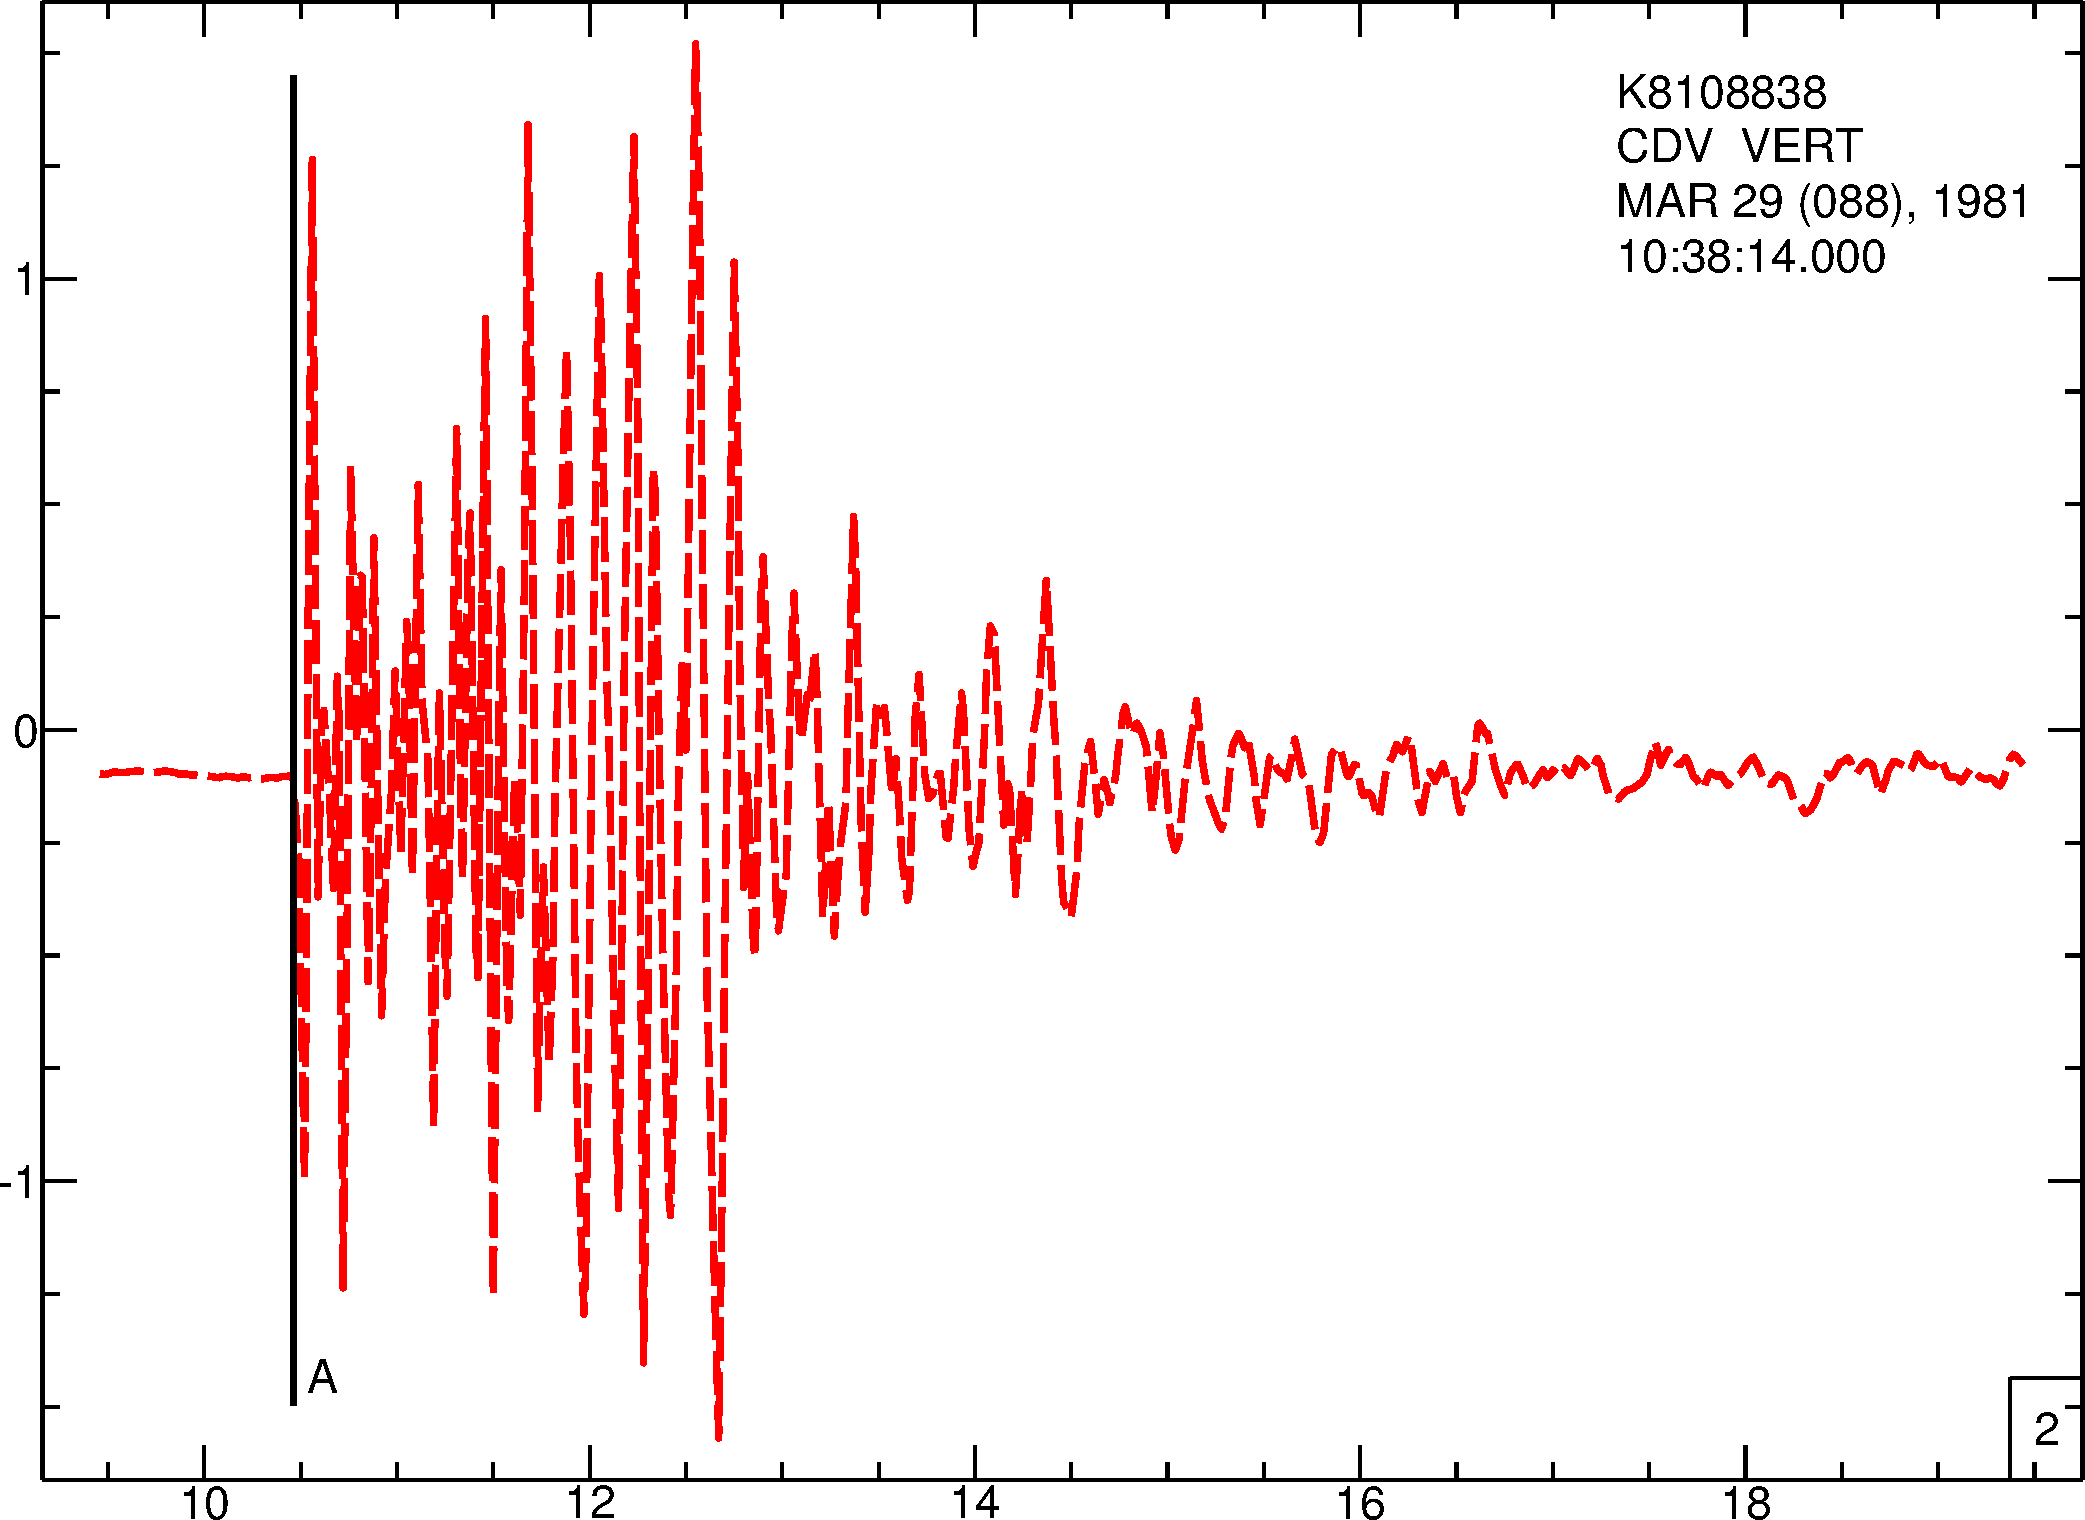
\includegraphics[width=0.7\textwidth]{attribution1}
\caption{线条属性}
\end{figure}

在绘制多个波形数据时,可以设置线条的属性按照某个列表递增。下面的命令一次绘制四个
波形文件,使每个数据的线型和颜色都按照默认列表递增。
\begin{SACCode}
SAC> dg sub teleseis ntkl.z nykl.z onkl.z sdkl.z
SAC> line incre
SAC> color black incre
SAC> p
\end{SACCode}

\begin{figure}[H]
\centering
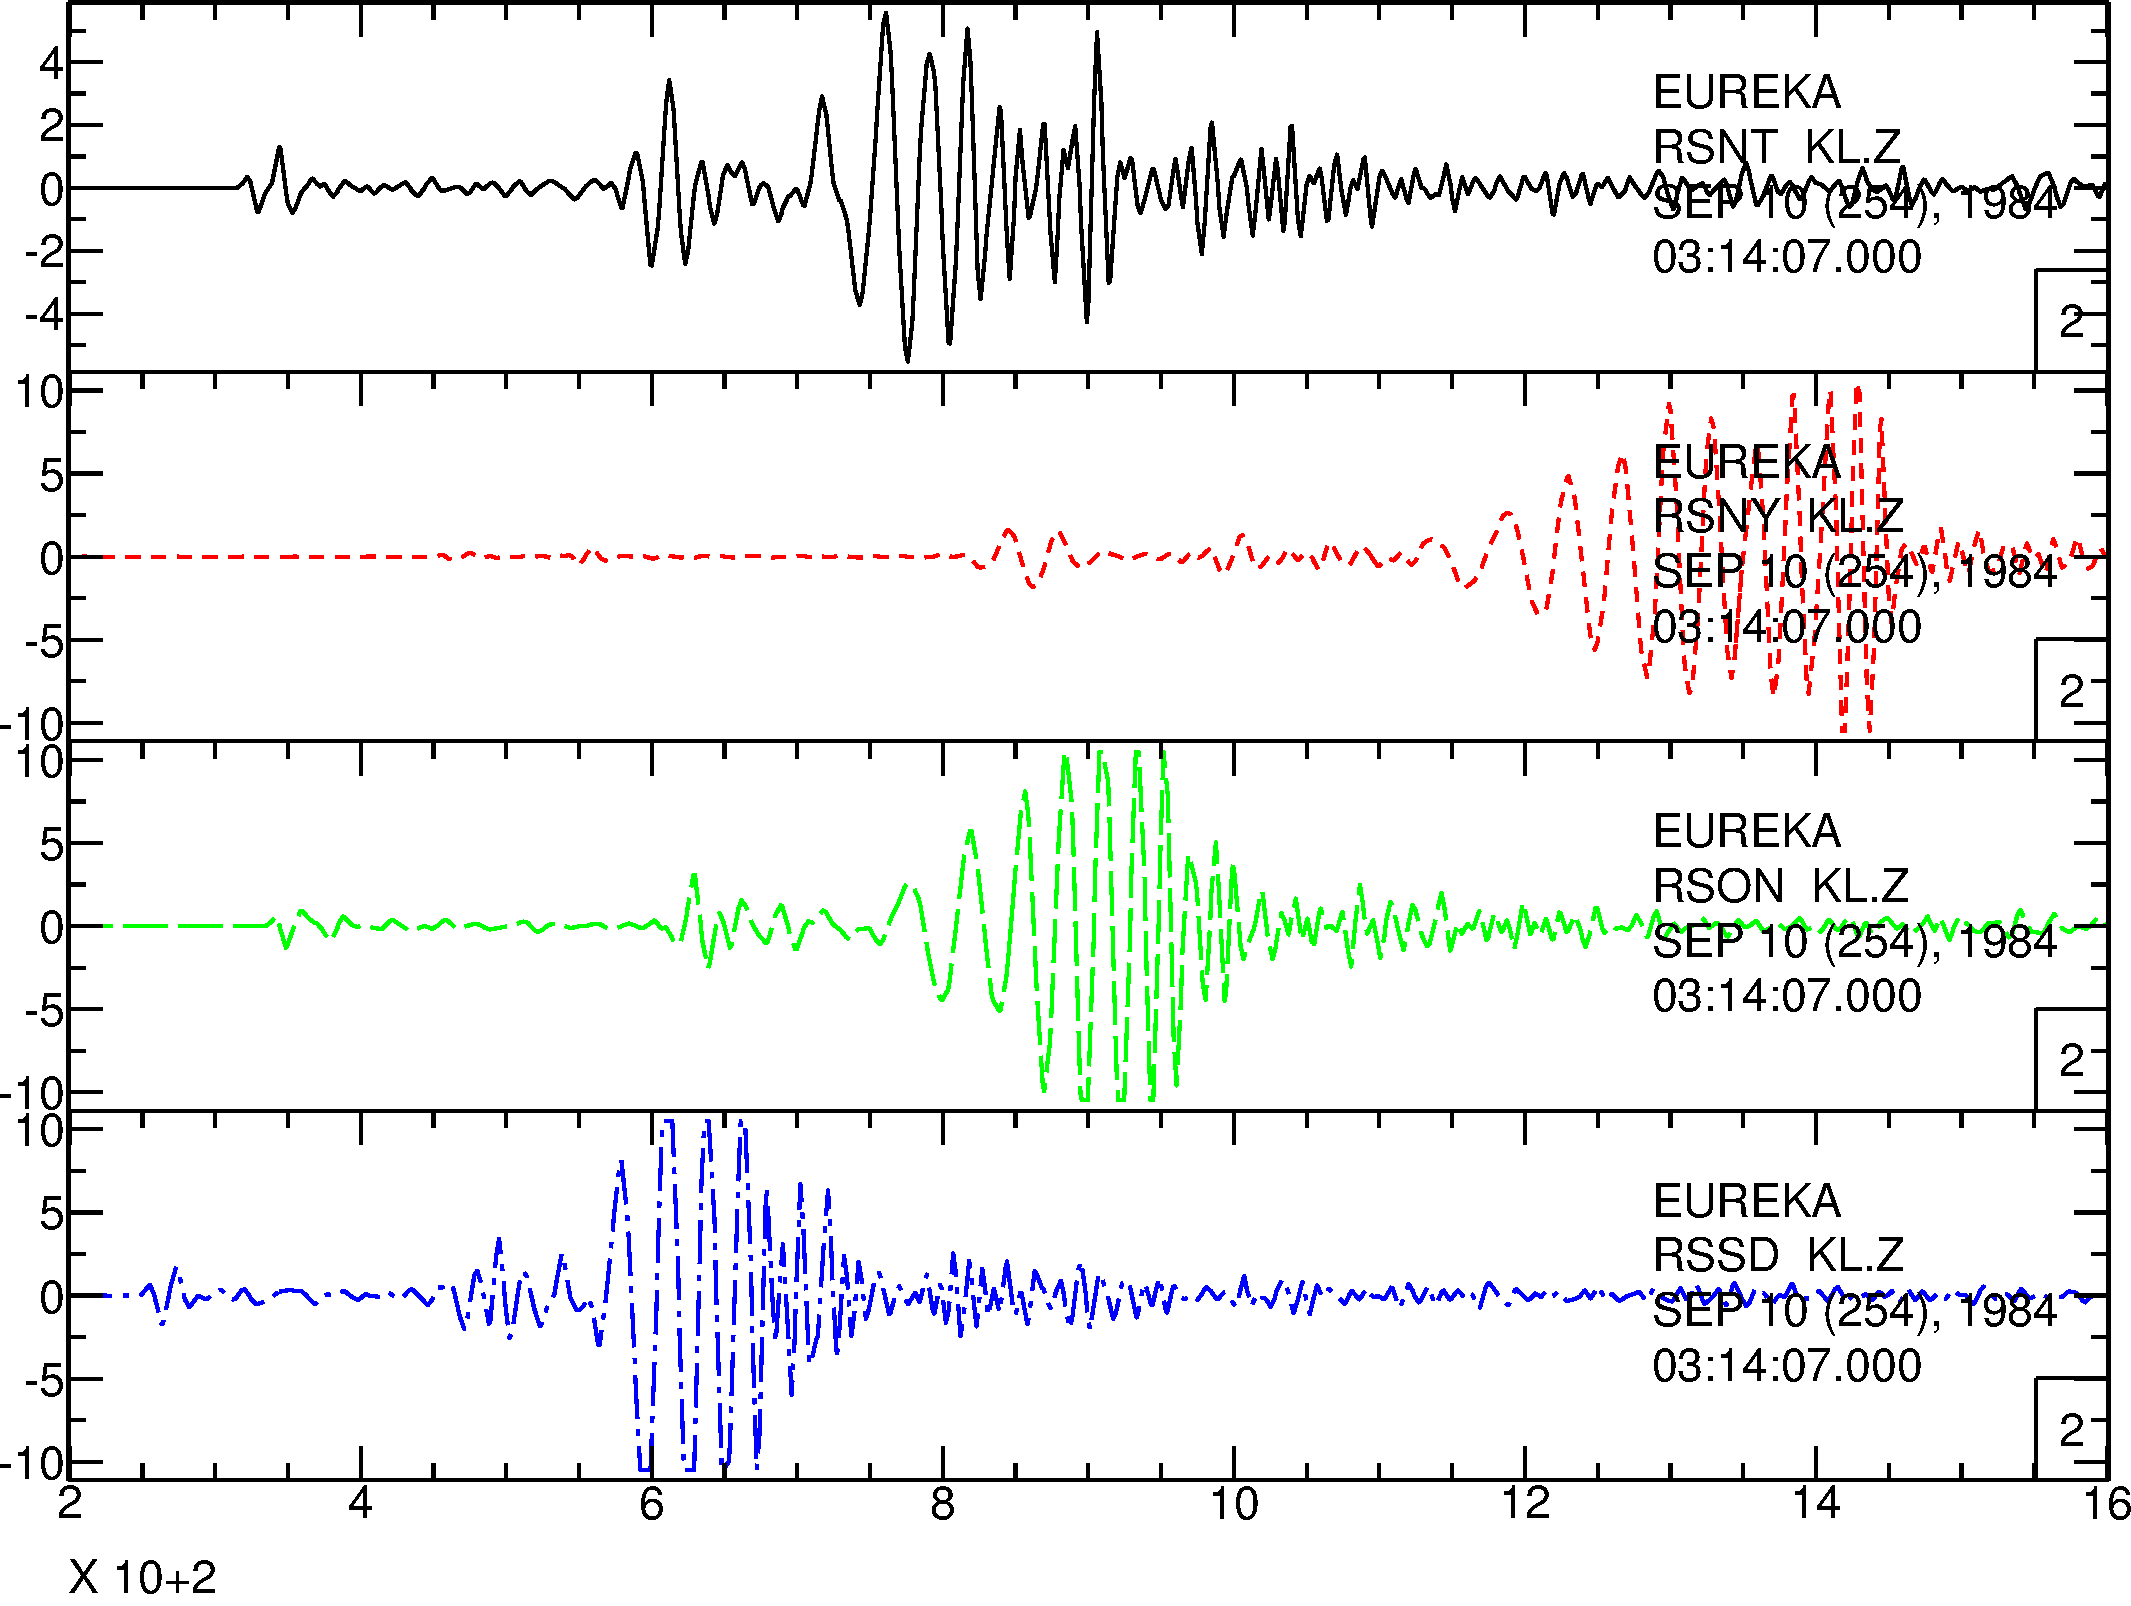
\includegraphics[width=0.7\textwidth]{attribution2}
\caption{线条属性递增}
\end{figure}

\nameref{cmd:line} 命令不仅可以设置线条的线型,同时可以对波形数据进行颜色填充:
\begin{SACCode}
SAC> fg seis
SAC> qdp off
SAC> rmean; rtr; taper
SAC> line 0 fill red/blue
SAC> p
\end{SACCode}

\begin{figure}[H]
\centering
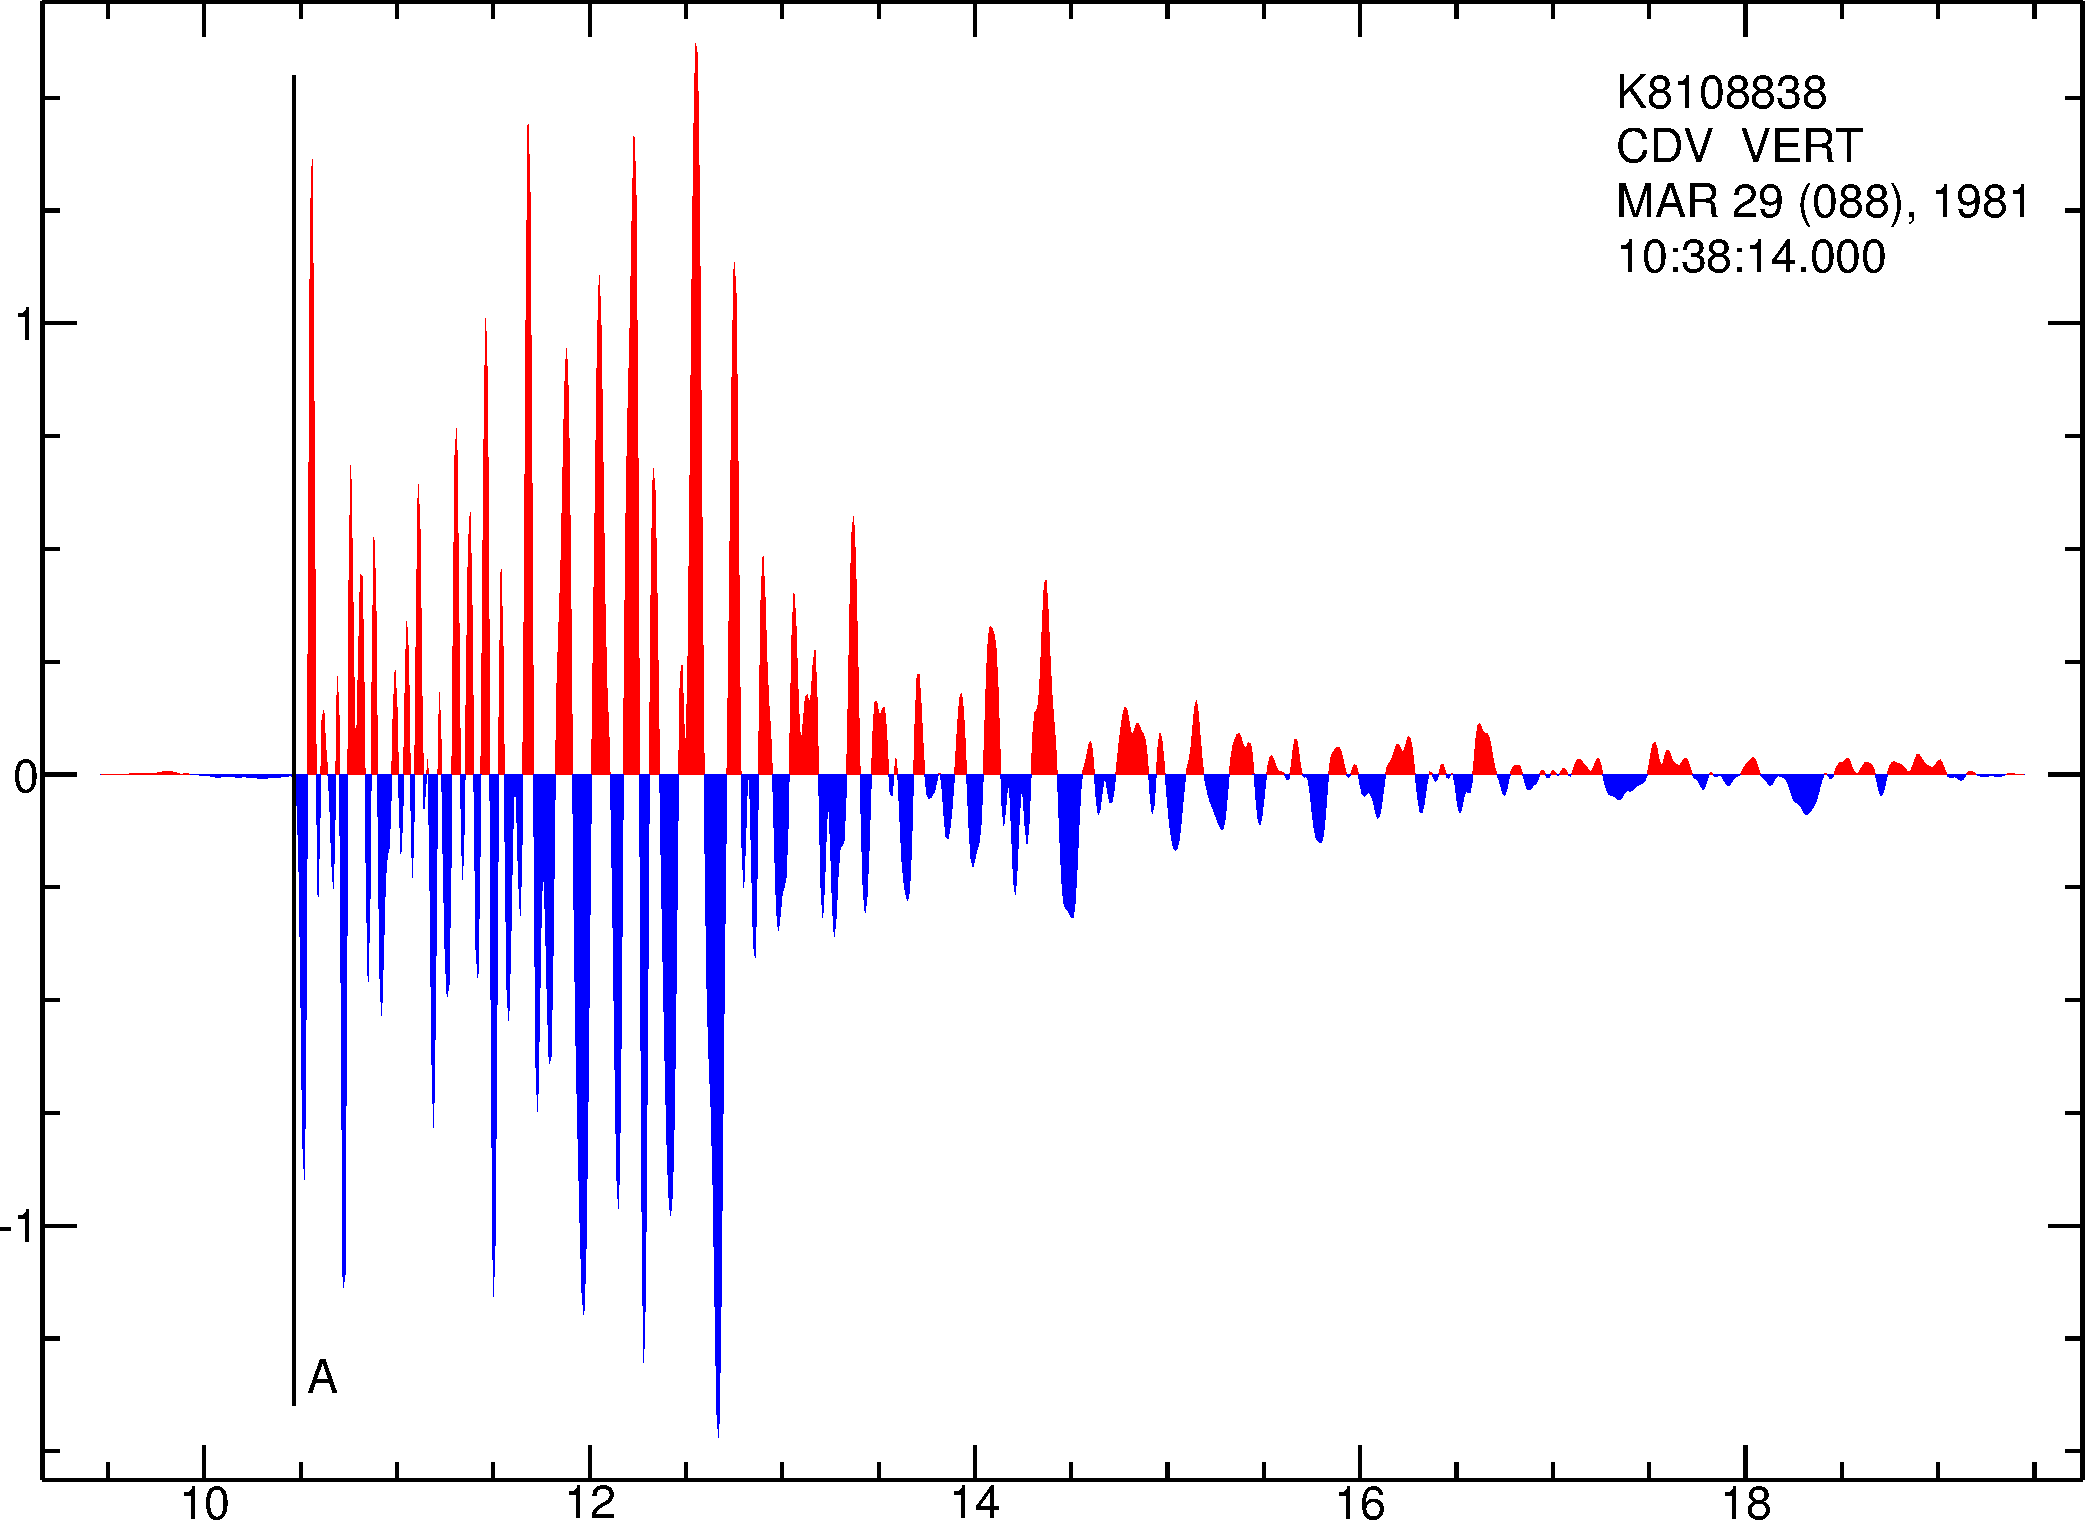
\includegraphics[width=0.7\textwidth]{linefill}
\caption{颜色填充图}
\end{figure}

\section{等值线图}
\label{sec:contour}
SAC中 \nameref{cmd:spectrogram} 等命令可以生成IXYZ数据(即3D数据),这种数据需要
用等值线图来展示。\nameref{cmd:contour} 命令用于等值线,\nameref{cmd:zcolors}、
\nameref{cmd:zlabels}、\nameref{cmd:zlevels}、\nameref{cmd:zlines}、\nameref{cmd:zticks}
分别用于控制等值线的颜色、标签、间距、线型以及刻度。

下面的例子中,读入了XYZ文件contourdata,从头段中找出Z数据的范围。
选择等值线范围为 \SI{700}{\km} 到 \SI{1150}{\km},增量为 \SI{25}{\km}。

选择包括四种线型的线型表,其中第一个为实线。这个列表将每四条等值线重复一次。
然后给等值线图起了个名字,最后绘制出来:
\begin{SACCode}
SAC> r ./contourdata
SAC> lh iftype depmin depmax

       IFTYPE = GENERAL XYZ (3-D) FILE
       DEPMIN = 6.977119e+02
       DEPMAX = 1.154419e+03
SAC> zlevels range 700 1150 increment 25
SAC> zlines list 1 2 3 4
SAC> title 'Katmai topography from survey data [inc = 25 km]'
SAC> contour
\end{SACCode}

\begin{figure}[H]
\centering
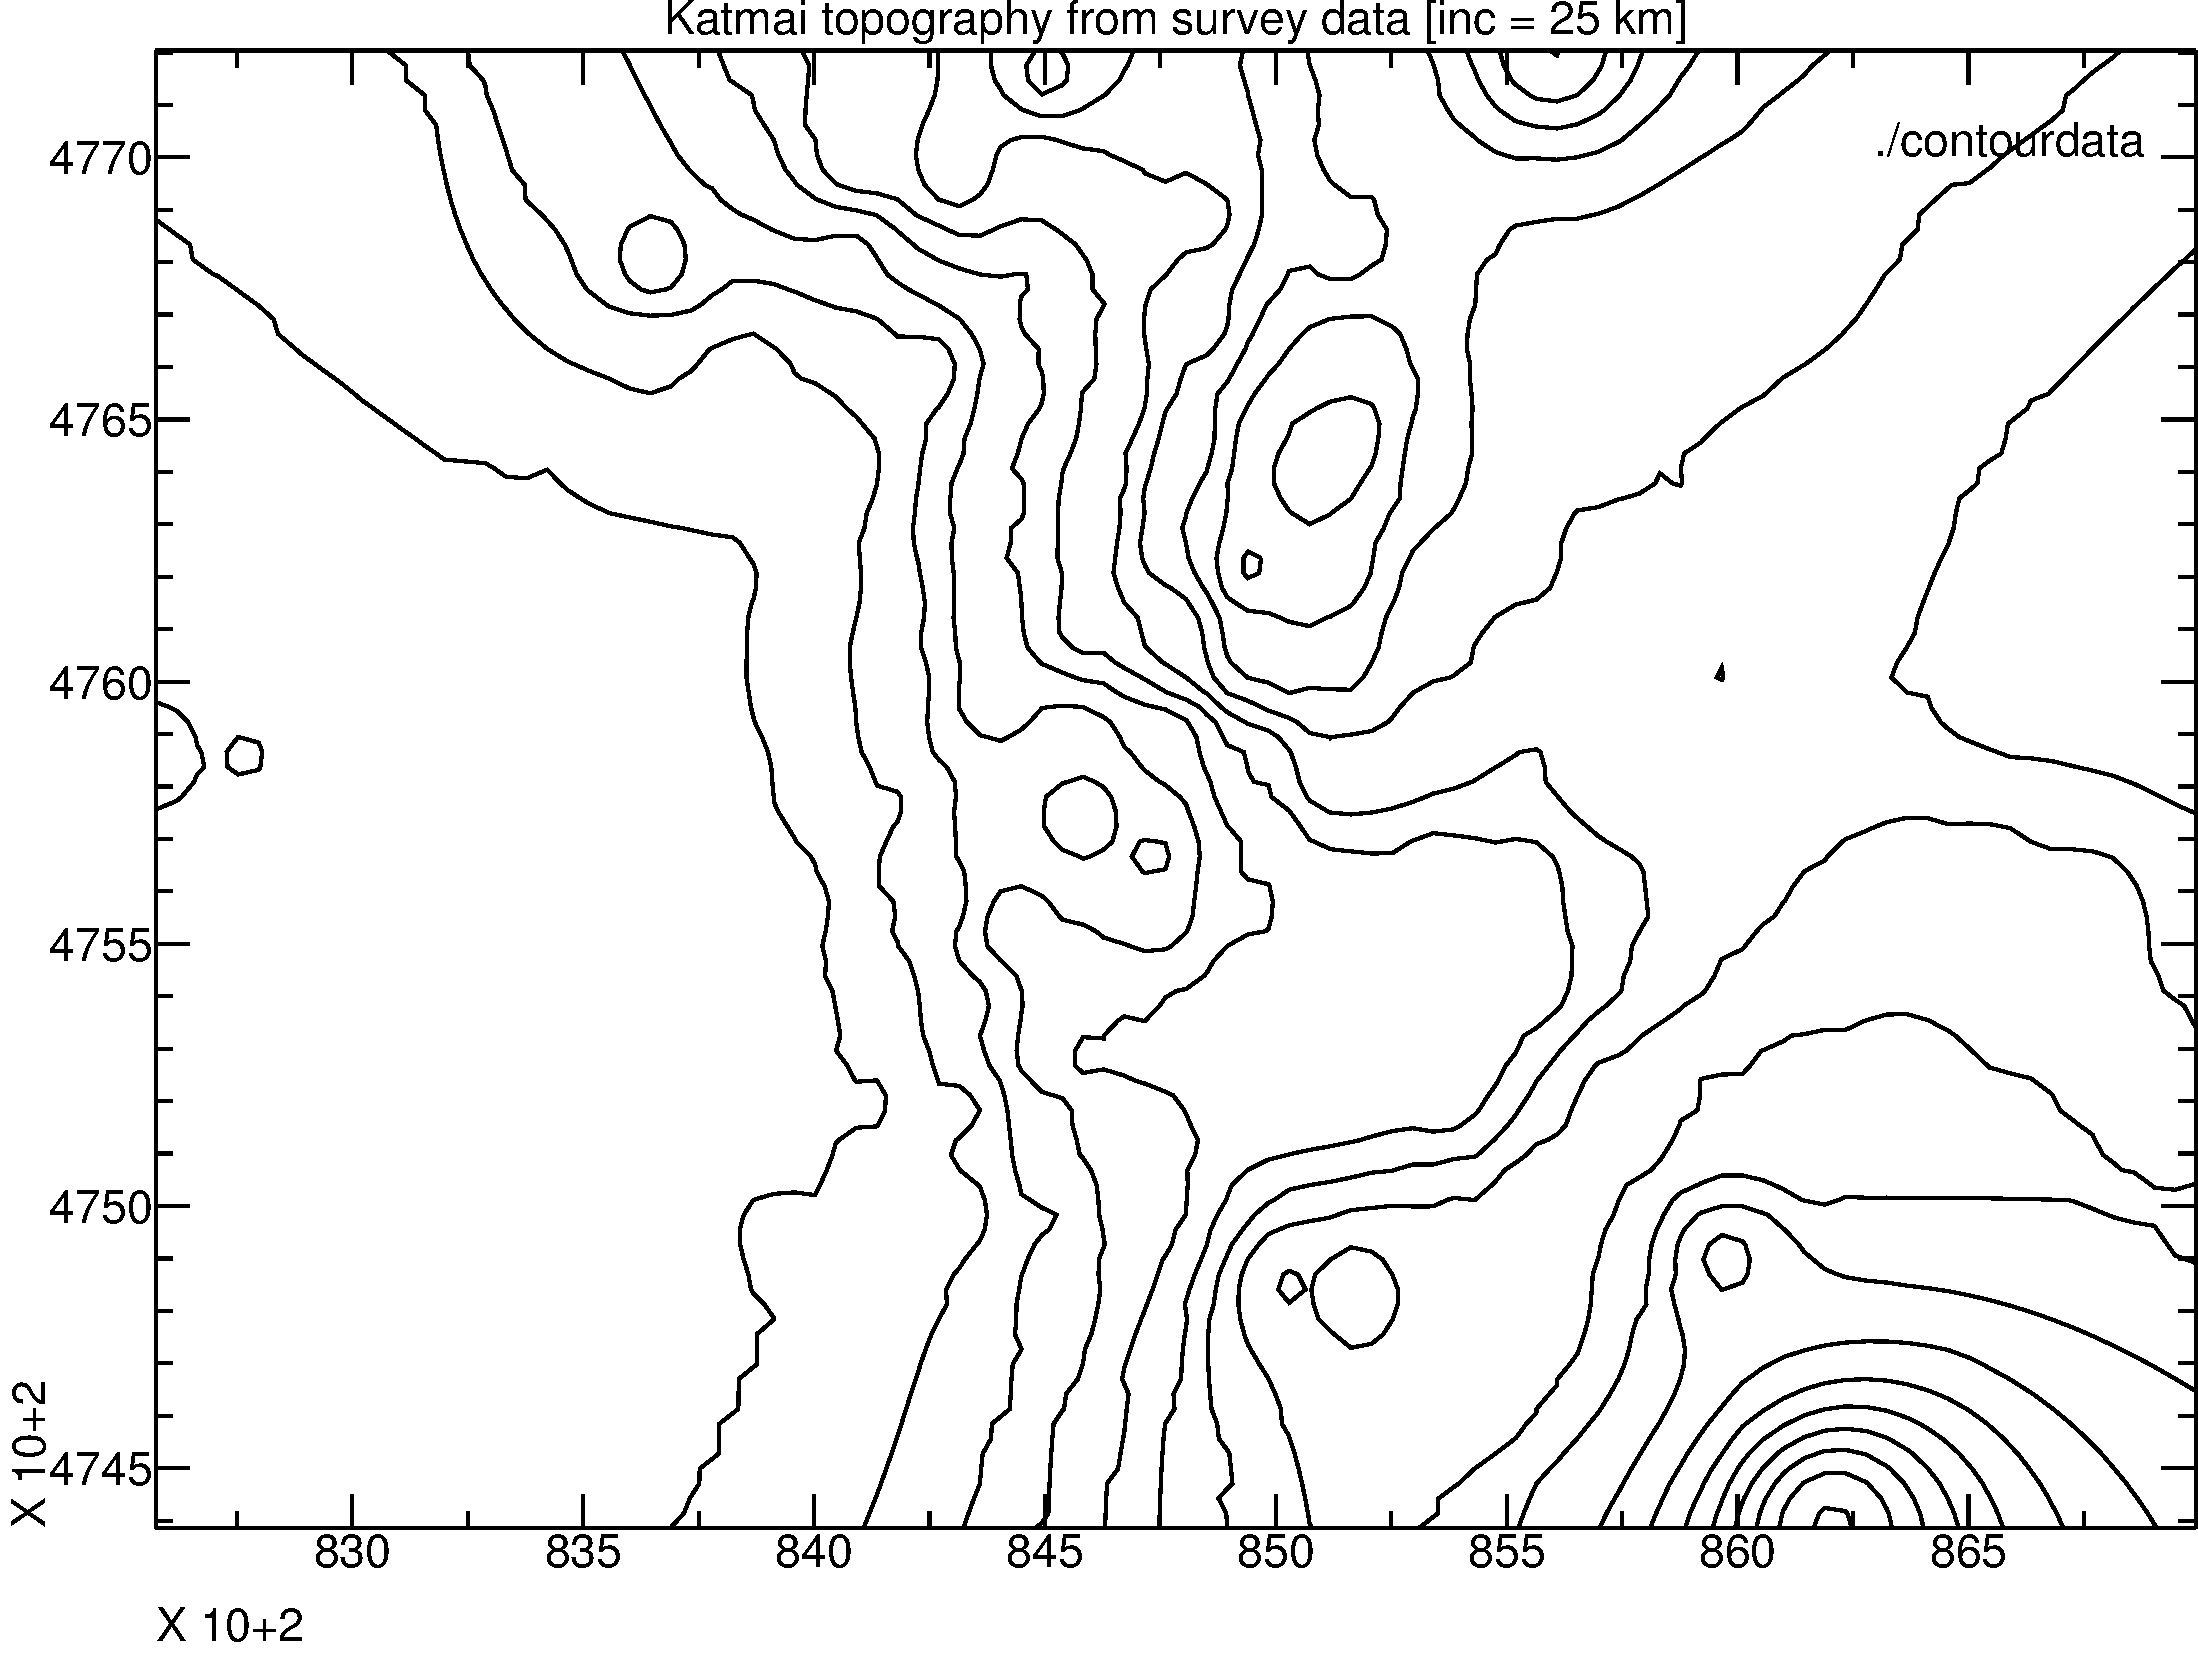
\includegraphics[width=0.9\textwidth]{contour1}
\caption{contour绘制等值线I}
\end{figure}

下面的例子中,使用同样的文件,但是显示选项不同。每四条等值线有一个整数标签。
每条等值线之间都有一个指向向下的箭头。所有等值线为实线型:
\begin{SACCode}
SAC> r ./contourdata
SAC> zlevels range 700 1150 increment 25
SAC> zlabels on list int off off off
SAC> zticks on direction down
SAC> zlines list 1
SAC> title 'Katmai topography from survey data [labels and ticks]'
SAC> contour
\end{SACCode}

\begin{figure}[H]
\centering
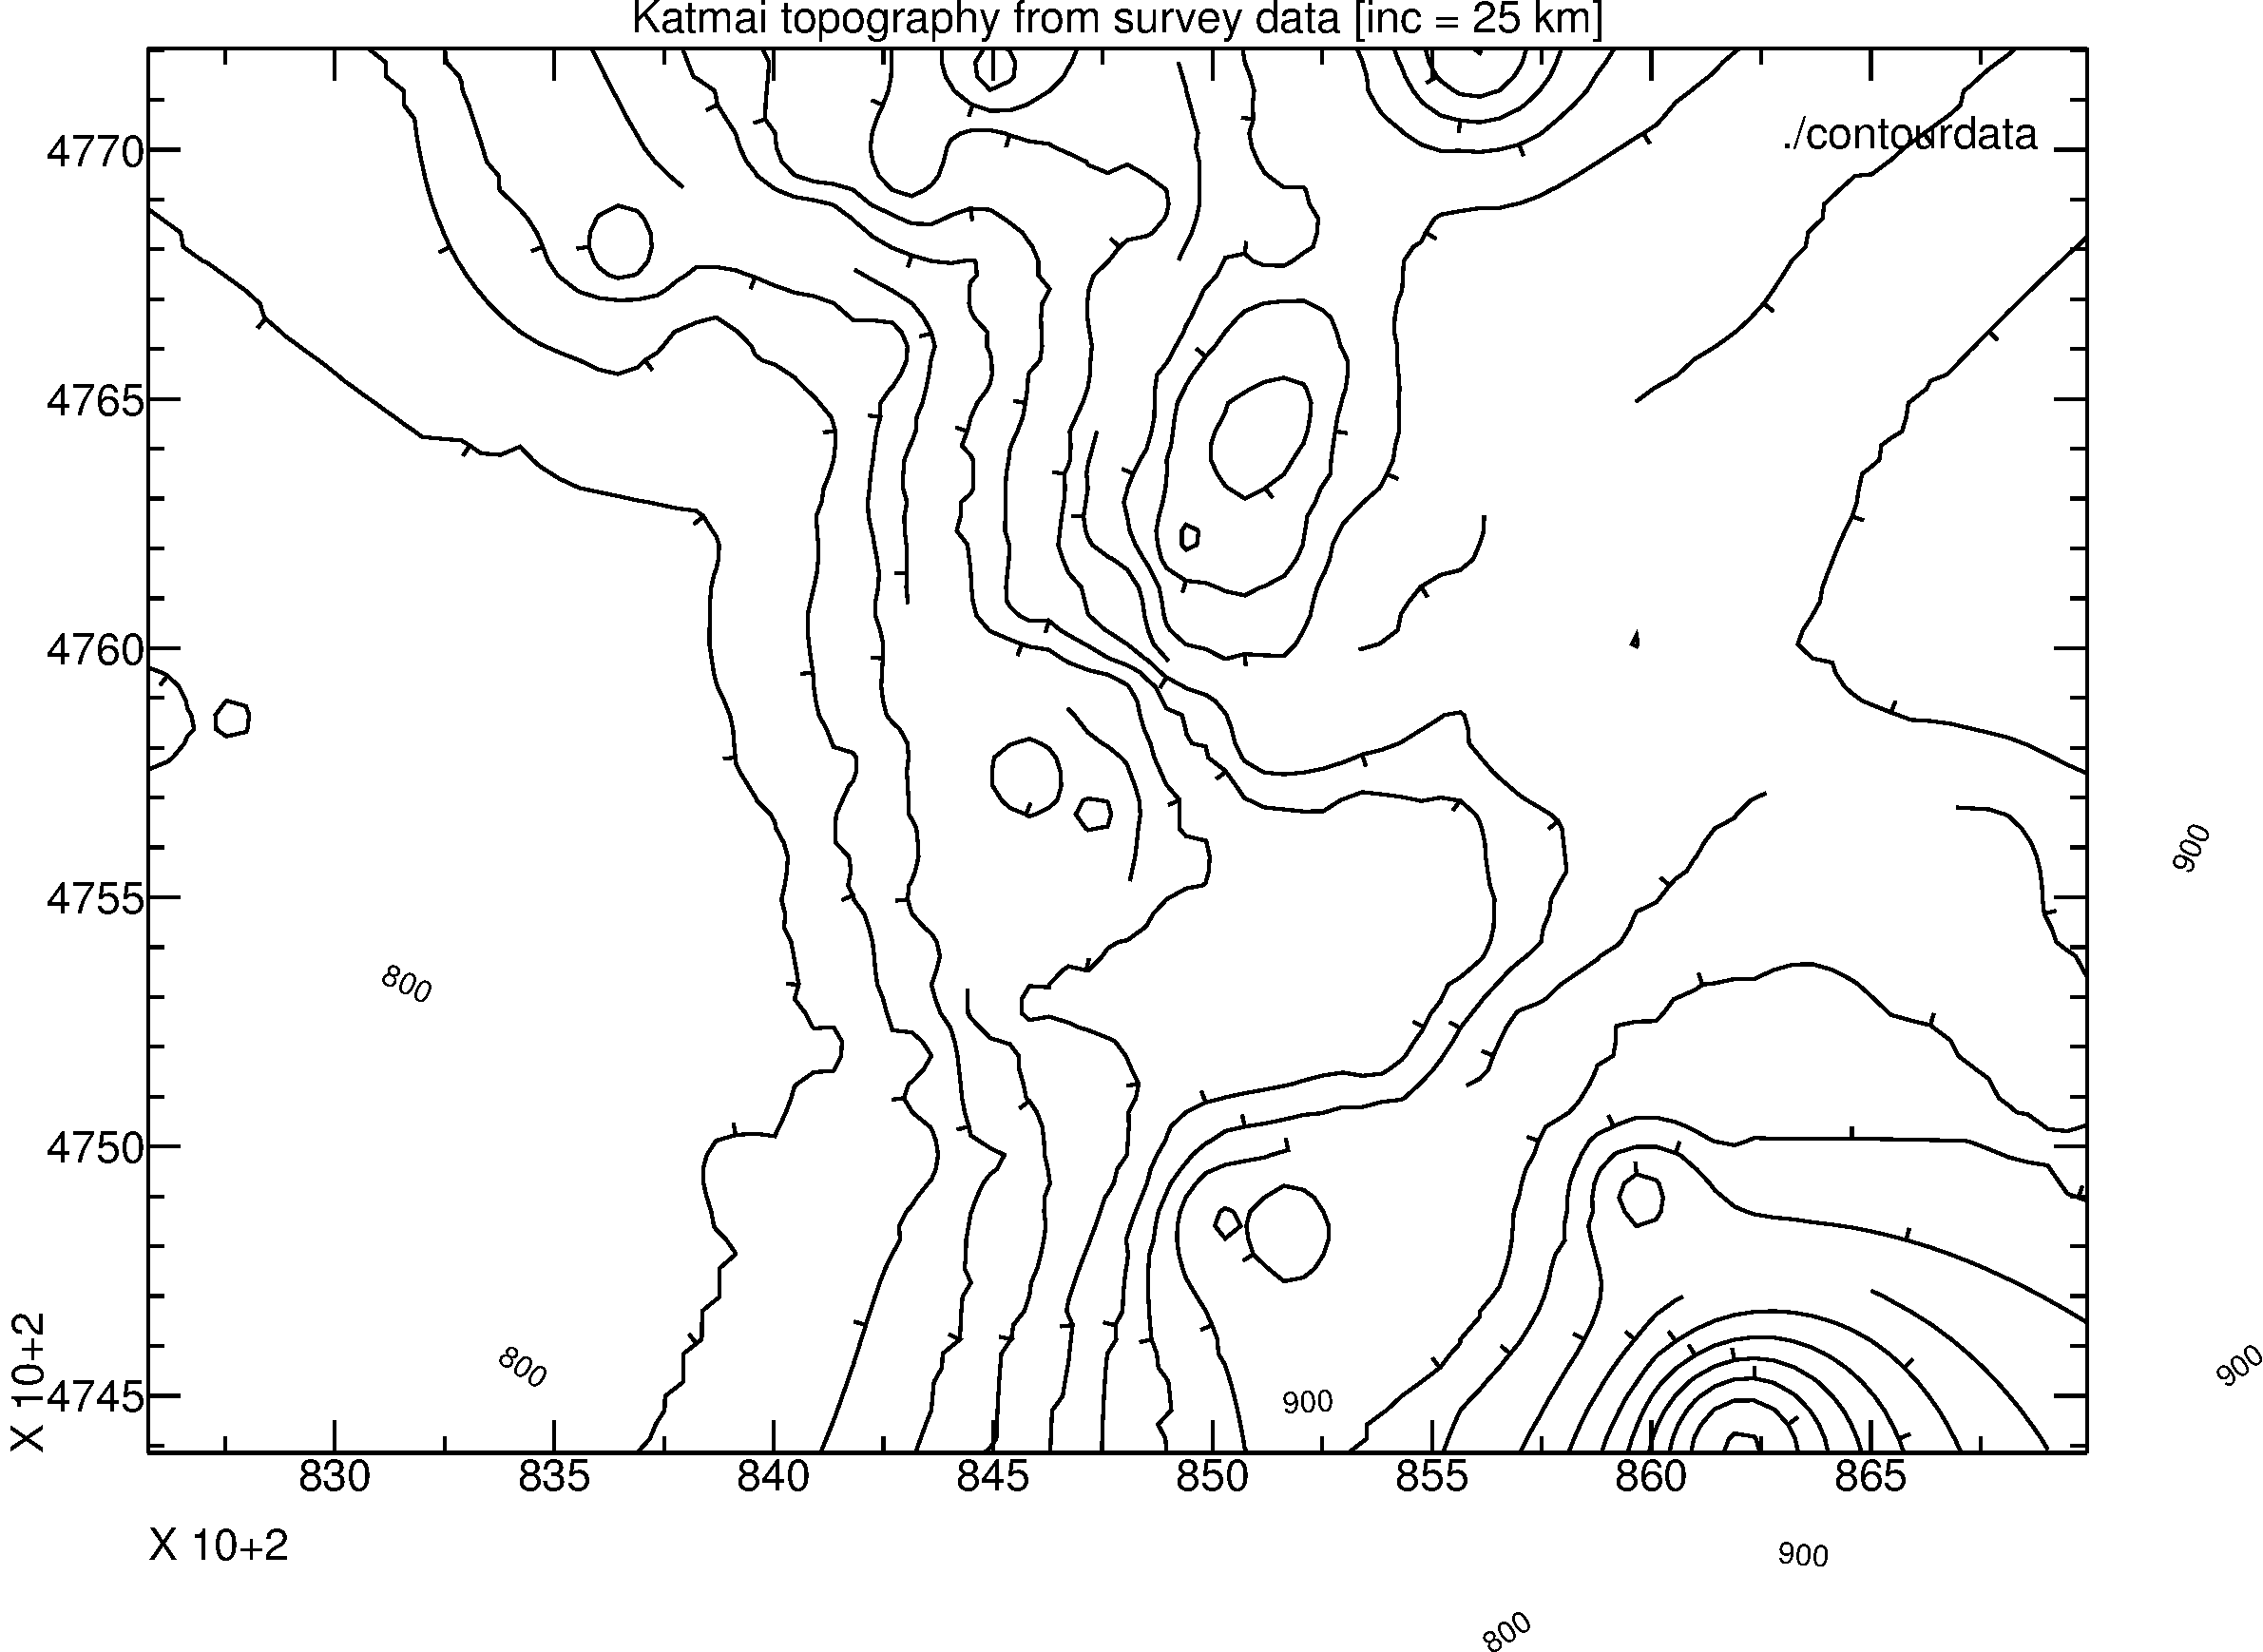
\includegraphics[width=0.9\textwidth]{contour2}
\caption{contour绘制等值线图II}
\end{figure}

\section{组合图}
\label{sec:composite-plots}

前面介绍的绘图命令五花八门,但无论是plot、plot1或是plot2,同一个窗口内绘制的
所有波形总是共用同一个X轴。实际绘图时,经常需要在一张图中绘制多个不同X轴的图,
即组合图。

SAC提供了绘制组合图的功能,这其中牵涉到一些新的概念,其中之一是~\verb+frame+。
一般而言,在执行绘图命令时会首先对整个窗口进行擦除。比如,先执行plot命令,窗口中
会显示出相应的波形,然后执行plot1命令,首先会将窗口中的已有图像全部擦除,再绘制
相应波形。

在frame中,每次执行绘图命令时,不会擦除窗口中的已有图像,从而实现了将多个命令的
绘图效果同时显示在一个窗口中。使用~\nameref{cmd:beginframe}~打开frame时,首先会
擦除整个窗口,进入``组合图模式'';当组合图绘制完成时,需要使用~\nameref{cmd:endframe}~命令关闭frame。

除了frame之外,在绘制组合图时还需要了解与窗口有关的几个概念,如图~\ref{fig:window-viewspace-viewport}:
\begin{itemize}
\item window:图形窗口。对于xwindows图形设备,window如图~\ref{fig:plot}~所示,
    其默认长宽比为11.0/8.5=1.294;对于sgf图形设备,可以认为window的大小即为A4纸张的大小。
\item viewspace:window内可以用于绘图的部分;
\item viewport:执行单个绘图命令时,图像的显示区域;
\end{itemize}

\begin{figure}[H]
\centering
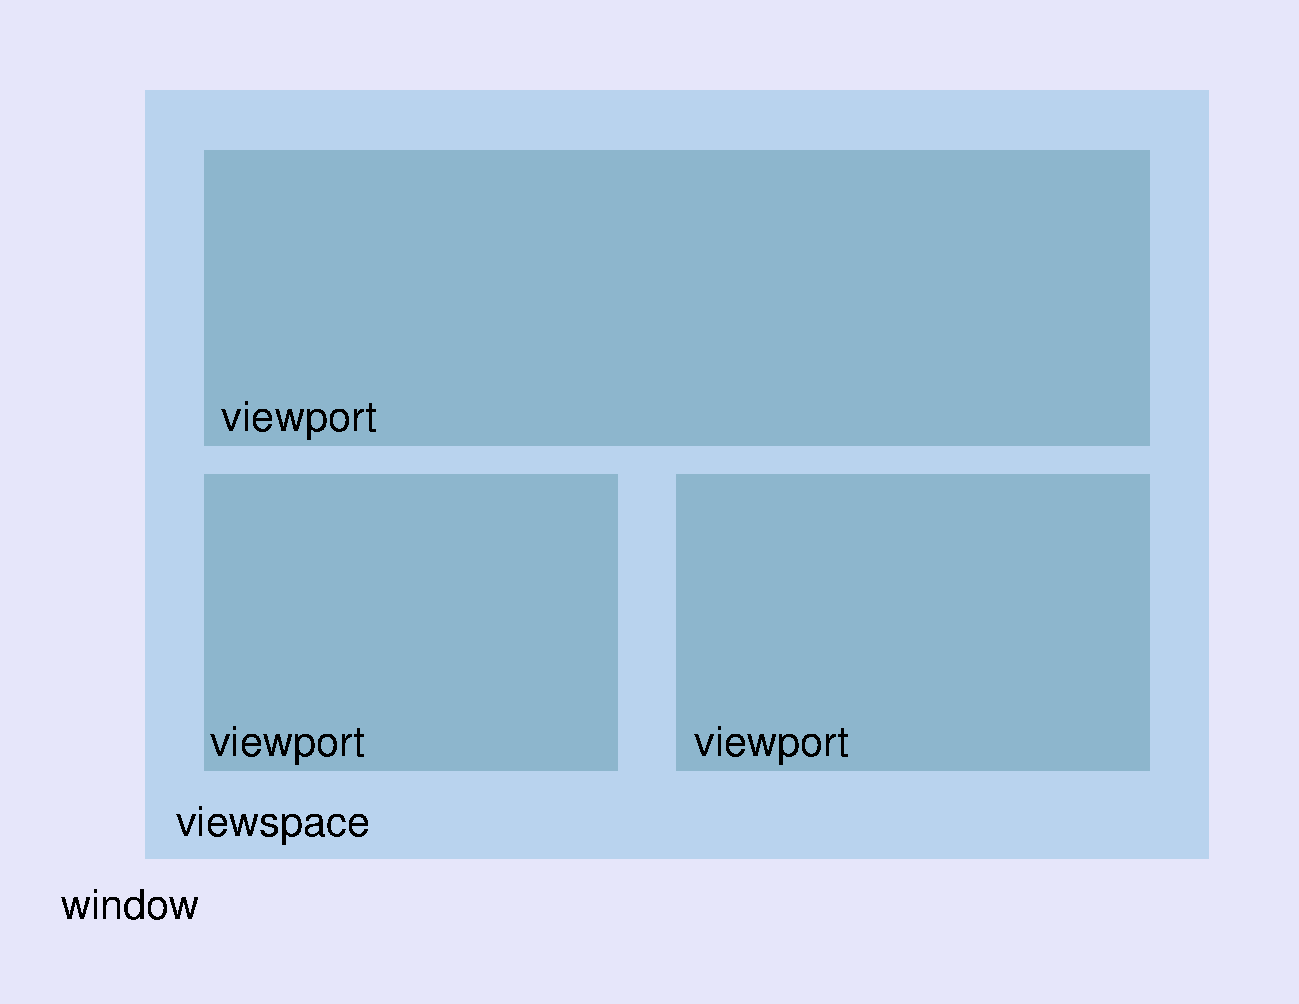
\includegraphics[width=0.8\textwidth]{viewspace-viewport}
\caption{window、viewspace和viewport}
\label{fig:window-viewspace-viewport}
\end{figure}

图~\ref{fig:window-viewspace-viewport}~中给出了window、viewspace、viewport的相关
关系。可以使用~\nameref{cmd:window}~命令设定窗口相对于整个屏幕的位置以及X、Y方向
的范围;\nameref{cmd:vspace}~用于设定整个绘图区的比例;\nameref{cmd:xvport}~和
\nameref{cmd:yvport}~则分别定义了单个绘图命令所能使用的X、Y方向的范围。

一个典型的组合图的绘制如下所示:
\begin{SACCode}
SAC> fg seis                        // 生成数据
SAC> beginframe                     // 打开frame,开始绘制组合图
SAC> xvport 0.1 0.9                 // 设定第一个绘图命令的viewport
SAC> yvport 0.7 0.9
SAC> title 'Seismic Trace'          // 设定标题
SAC> fileid off                     // 不显示文件id
SAC> qdp off
SAC> p
SAC> fft wmean                      // FFT
SAC> xvport .1 .45                  // 设定第二个绘图命令的viewport
SAC> yvport .15 .55
SAC> title 'Amplitude Response (linlog)'
SAC> ylim 1e-5 1                    // Y轴范围
SAC> psp am linlog                  // 绘制振幅谱(linlog)
SAC> xvport .55 .9                  // 设定第三个绘图命令的viewport
SAC> title 'Amplitude Response (loglog)'
SAC> xlim 1 60
SAC> psp am loglog                  // 绘制振幅谱(loglog)
SAC> endframe                       // 关闭frame
\end{SACCode}

\begin{figure}[H]
\centering
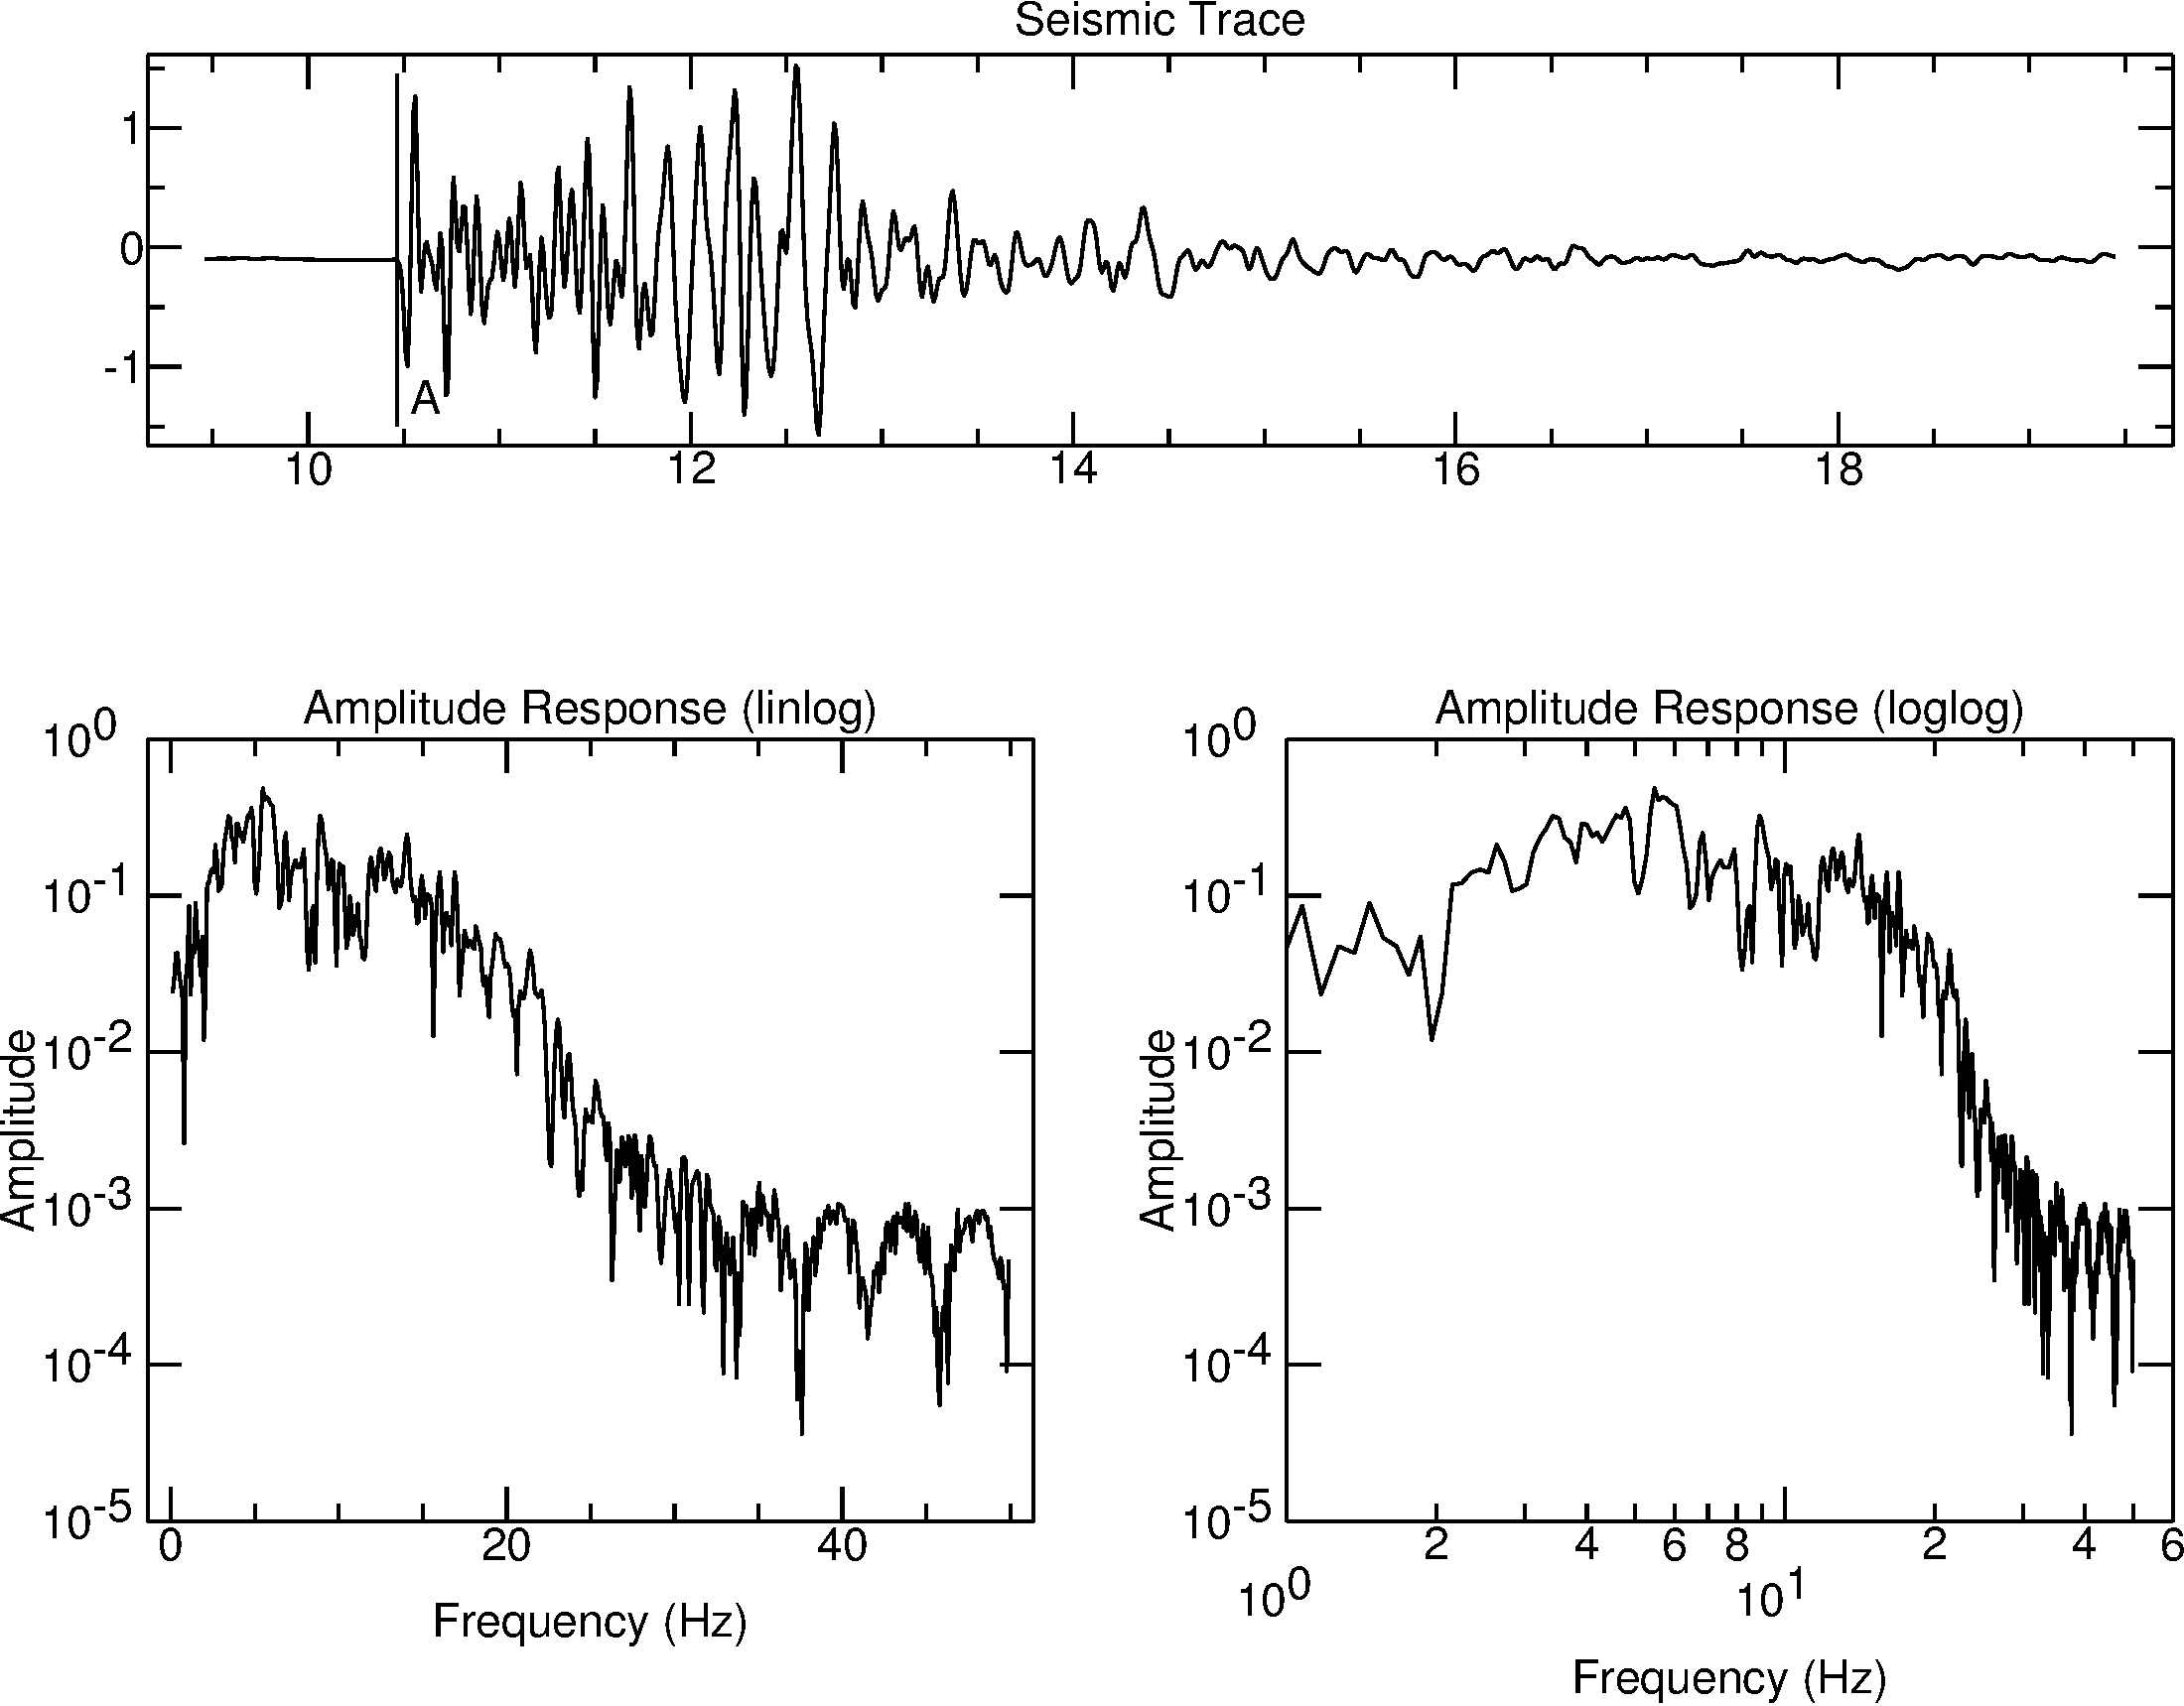
\includegraphics[width=0.9\textwidth]{composite-plot}
\caption{绘制组合图}
\label{fig:composite-plot}
\end{figure}

\section{图像保存}
\label{sec:save-image}

\subsection{xwindows}
xwindows是SAC中最常用绘图设备,对于震相拾取等交互式操作更是必不可缺。
\begin{SACCode}
SAC> fg seis
SAC> bd x       // begindevice xwinows,可省略
SAC> p          // 绘图
SAC> ed x       // enddevice xwindows,可省略
SAC> q
\end{SACCode}

对于xwindows,最简单的保存图像的方式是截图,常用的工具包括gnome下的screenshot或者
ImageMagick的 \texttt{import} 命令。

\subsection{sgf}
SGF图形设备会将图像信息保存到SGF文件中。其使用方式为:``启用sgf图形设备''$\rightarrow$
``绘图到sgf''$\rightarrow$``关闭sgf设备,退出SAC''$\rightarrow$``将sgf文件转换为其它格式''。
\begin{SACCode}
SAC> fg seis
SAC> bd sgf         // 启动sgf设备,不可省略
SAC> p
SAC> ed sgf         // 关闭sgf设备,可省略
SAC> q
$ ls
f001.sgf            // 生成sgf文件
\end{SACCode}

生成的sgf文件可以通过sgftops等命令转换为其它图像格式,在``\nameref{sec:sgftops}''中会介绍,
也可以使用sgftox直接将sgf文件显示在绘图窗口中。

\subsection{PS和PDF}
自101.5之后,SAC加入了 \nameref{cmd:saveimg} 命令,可以将当前xwindow或sgf图形设备中的图像保存到
其它ps或pdf格式的图像文件中,以获得更高质量的绘图效果。
\footnote{该命令也支持输出为png和xpm格式,但png和xpm为位图图像格式,精度不够,
且依赖于其它函数库,因而不推荐使用。}

\begin{SACCode}
SAC> fg seis
SAC> p                      // 首先在xwindows上绘图
SAC> saveimg foo.ps         // 将xwindows上的图像保存到foo.ps中
save file foo.ps [PS]
SAC> q
\end{SACCode}

\subsection{pssac}
pssac是Prof. Lupei Zhu写的用于绘制SAC文件的C程序。该程序利用了GMT的PS绘图库,
直接读取SAC文件并绘制到PS文件中。得益于GMT的PS库的灵活性,利用pssac可以绘制出
超高质量的复杂图像。具体参见``\nameref{sec:pssac}''一节。

\subsection{小结}
\begin{itemize}
\item 在xwindows上绘图简单省事,直接截图的效果较差,仅可用于非正式的演示;
\item sgf转换为其它图像格式稍显麻烦,但适合在脚本中批量做图;
\item saveimg生成图像文件质量相对较高,可以满足大多数需求;
\item pssac功能强大,在一般绘图以及复杂图像时非常有用,适合在发表文章时使用;
\end{itemize}

\section{图像格式转换}
\label{sec:format-conversion}

SAC中的图像可以保存为SGF、PS和PDF格式,有些时候会需要将其转换为其他图像格式,比如JPG或PNG。

\texttt{convert} 是Linux下的一个功能强大的图像格式转换工具。如果你的系统里没有这个命令,你可以通过安装 \texttt{ImageMagick} 来获取该命令。

convert命令的选项众多,这里只说其中几个常用的选项:

\begin{itemize}
\item \texttt{-trim} :切边,即将图像周围多余的白边切除;
\item \texttt{-density}  \textit{width}\texttt{x}\textit{height}:设置图像精度,一般情况下,设置width为300即可,height可以不指定。
\item \texttt{-rotate}  \textit{degree}:图像旋转的角度;
\end{itemize}

下面给出一个简单的例子:

\begin{minted}{console}
    convert -trim -density 300x300 -rotate 90 image.ps image.png
\end{minted}

\chapter{SAC编程}
\label{chap:sac-programming}
\input{macros/intro-to-sac-programming}
\section{引用头段变量值}
前面已经介绍了SAC中的很多头段变量,也知道如何使用 \nameref{cmd:listhdr} 查看头段
变量的值,lh命令的输出对于人来说很直观,但是对于机器来说却很不友好。有些时候需要
直接使用头段变量的值,这就需要一些特殊的技巧。

最常见的情况是第 \pageref{code:origin-time} 页给出的例子。
在使用``\texttt{ch o gmt}''指定发震
时刻后,需要获取头段变量o的值,对该值取负值,并用于``\texttt{ch allt}''中。

本例中,需要先获取头段变量o的值,再将其值用于其它命令中,准确的说这叫变量
值的引用。在SAC命令中引用头段变量的值有两种方式,
分别是``\verb|&fname,header&|''和``\verb|&fno,header&|''\footnote{实际上,
SAC官方文档给出的引用方式中没有末尾的 \verb|&| 符号,仅当
一些特殊的情况下才使用,这样容易使得整个语法混乱不堪,所以这里采用了另外一种引用
方式。所有示例均已通过测试。}。

fname和fno都唯一指向了内存中的某个波形数据,其中fname表示文件名,fno表示文件号
(即内存中的第几个文件,索引值从1开始),header则为头段变量名。

下例展示了如何通过两种方式引用头段变量的值:
\begin{SACCode}
SAC> fg seis
SAC> w seis.SAC
SAC> r ./seis.SAC               // 注意"./"
SAC> lh kevnm o stla            // 查看三个头段变量的值

     kevnm = K8108838
         o = -4.143000e+01
      stla = 4.800000e+01
SAC> echo on processed          // 打开回显,显示处理信息
SAC> ch kuser0 &1,kevnm&        // 通过文件号引用头段变量kevnm
 ==>  ch kuser0 K8108838        // 实际执行的效果
SAC> ch user0 &./seis.SAC,o&    // 利用文件名,引用头段变量o
 ==>  ch user0 -41.43
SAC> ch user1 &seis.SAC,stla&   // 文件名少了"./"
 ERROR 1363: Illegal data file list name: seis.SAC
SAC> lh kuser0 user0 user1

     kuser0 = K8108838
     user0 = -4.143000e+01
\end{SACCode}

在通过文件名指定波形数据时要注意:SAC记录的是文件的全路径。一般情况下,使用
文件号会更方便些。

\section{黑板变量}
既然是SAC编程,就必然少不了变量,SAC中的变量称之为黑板变量。

黑板变量是SAC中用于临时储存和取回信息而设计的。
黑板变量不需要声明即可直接使用,可以用 \nameref{cmd:setbb} 和 \nameref{cmd:evaluate}
命令给黑板变量赋值,用 \nameref{cmd:getbb} 获取黑板变量的值。也可以用 \nameref{cmd:writebbf}
将黑板变量保存在磁盘文件中,然后使用 \nameref{cmd:readbbf} 命令重新将这些变量读入SAC中。


引用黑板变量的值的方式为:``\verb|%bbvname%|'',其中bbvname为黑板变量的变量名。

\begin{SACCode}
SAC> echo on processed
SAC> fg seis
SAC> p
SAC> setbb low 2.45         // 黑板变量low=2.45
SAC> setbb high 4.94        // 黑板变量high=4.94
SAC> bp c %low% %high%      // 引用黑板变量low和high的值作为滤波的频带
 ==>  bp c 2.45 4.94        // echo on processed 显示代入值后的命令
SAC> p
SAC> getbb low high         // 查看黑板变量的值
 low = 2.45
 high = 4.94
\end{SACCode}

下例展示了如何将黑板变量写入磁盘文件,等需要时再从磁盘文件中获取:
\begin{SACCode}
$ sac
SAC> setbb var1 10          // 整型
SAC> setbb var2 "text"      // 字符串
SAC> setbb var3 0.2         // 浮点型
SAC> wbbf bbf.file          // 写入到文件
SAC> q
$ ls
bbf.file
$ sac
SAC> readbbf ./bbf.file
SAC> getbb
 NUMERROR = 0
 SACERROR = 'FALSE'
 SACNFILES = 0
 VAR1 = 10
 VAR2 = 'text'
 VAR3 = 0.2
SAC> getbb var2 var3
 var2 = 'text'
 var3 = 0.2
SAC> q
\end{SACCode}

\section{内联函数}

内联函数是SAC实现的一些函数,其可以在SAC命令中使用。在执行命令时,内联函数会首先被
调用,内联函数的结果将替代命令中的内联函数的位置。

SAC提供了如下几类内联函数:
\begin{itemize}
\item 算术运算符;
\item 常规算术运算函数;
\item 字符串操作函数;
\item 其他函数;
\end{itemize}

所有的内联函数的共同形式是:``\texttt{(func)}'',其中func为内联函数名。某种程度
上,内联函数与前面说到头段变量(``\verb|& &|'')和黑板变量(``\verb|% %|'')类似,
可以认为是通过``\texttt{( )}''引用了内联函数的结果或值。

内联函数支持嵌套,目前最多可以嵌套10层。

\subsection{算术运算符}
算术运算符即常规的加减乘除运算符,但又有不同,其一般形式如下:
\begin{SACCode}
    ( number operator number )
\end{SACCode}
所有的操作数都被认为是实型的,所有的算术运算都按照双精度浮点型进行运算;

SAC支持的操作符是包括:``\texttt{ +  -  *  /  ** }''。

看几个简单的例子:
\begin{SACCode}
SAC> echo on
SAC> setbb var1 4+7             // 忘记加括号了!"4+7"被当成了字符串
 setbb var1 4+7
SAC> setbb var2 (4+7)
 setbb var2 (4+7)
 ==>  setbb var2 11             // 4+7=11
SAC> setbb var3 (4+7/3)         // 优先级正确
 setbb var3 (4+7/3)
 ==>  setbb var3 6.33333
SAC> setbb var4 ((4+7)/3)       // 括号改变优先级
 setbb var4 ((4+7)/3)           // 可以看作是内联函数的嵌套
 ==>  setbb var4 3.66667
SAC> setbb var1 ( ( 4 + 7 ) / 3 )   // 支持空格
 setbb var1 ( ( 4 + 7 ) / 3 )
 ==>  setbb var1 3.66667
\end{SACCode}

\subsection{常规算术运算函数}
SAC提供了20个常规算术运算函数,其基本形式为``\texttt{(func arg1 arg2 ...)}''。
具体函数如表 \ref{table:regular-arithmetic-functions} 所示。

\begin{table}[!ht]
\centering
\ttfamily
\small
\caption{常规算数运算函数}
\label{table:regular-arithmetic-functions}
\begin{tabular}{lll}
	\toprule
	命令	&	语法	&	功能	\\
	\midrule
	add		&	( add v1 v2 ... vn )	    &	v1+v2+...+vn	\\
	subtract&	( subtract v1 v2 ... vn )   &	v1-v2-...-vn	\\
	multiply&	( multiply v1 v2 ... vn )   &	v1*v2*...*vn	\\
	divide	&	( divide v1 v2 ... vn )	    &	v1/v2/.../vn	\\
	absolute&	( absolute v )			    &	取绝对值	\\
	abs     &	( abs v )			        &	取绝对值	\\
	power	&	( power v )				    &	取10的v次方     \\
	alog10	&	( alog10 v)				    &	以10为底取v的对数	\\
	alog	&	( alog v)				    &	取v的自然对数	\\
	exp	    &	( exp v)				    &	取e的v次方	\\
	sqrt	&	( sqrt v) 				    &	求v的平方根	\\
	pi		&	( pi )					    &	返回pi值	\\
    sine    &	( sine v )				    &	正弦(v为弧度,下同)\\
	cosine	&	( cosine v )				&	余弦	\\
    tangent	&	( tangent v )			    &	正切	\\
	arcsine	&	( arcsine v )			    &	反正弦	\\
	arccosine&	( arccosine v ) 			&	反余弦	\\
	arctangent&	( arctangent v )			&	反正切	\\
    integer &	( integer v )			    &	取整	\\
	maximum	&	( maximum v1 v2 ... vn )	&	求最大值	\\
	minimum	&	( minimum v1 v2 ... vn )	&	求最小值	\\
	\bottomrule
\end{tabular}
\end{table}

演示如下:
\begin{SACCode}
SAC> echo on processed
SAC> setbb var1 (add 1 3 4)         // 1+3+4
 ==>  setbb var1 8
SAC> setbb var2 (subtract 1 3 4)    // 1-3-4
 ==>  setbb var2 -6
SAC> setbb var3 (multiply 1 3 4)    // 1*3*4
 ==>  setbb var3 12
SAC> setbb var4 (divide 1 3 4)      // 1/3/4
 ==>  setbb var4 0.0833333
SAC> setbb var5 (absolute -5.1)     // abs(-5.1)
 ==>  setbb var5 5.1
SAC> setbb var6 (power 5)           // 10^5
 ==>  setbb var6 100000
SAC> setbb var7 (alog10 10000)      // log10(10000)
 ==>  setbb var7 4
SAC> setbb var8 (alog 10000)        // ln(10000)
 ==>  setbb var8 9.21034
SAC> setbb var9 (exp 5)             // e^5
 ==>  setbb var9 148.413
SAC> setbb var10 (sqrt 9)           // sqrt(9)
 ==>  setbb var10 3
SAC> setbb var11 (pi)               // PI
 ==>  setbb var11 3.14159
 SAC> setbb var12 (sine (pi/6))     // sin(30)
 ==>  setbb var12 0.5
SAC> setbb var13 ((arcsine 0.5)*180/(pi))
 ==>  setbb var13 30
SAC> setbb var14 (integer 3.11)
 ==>  setbb var14 3
SAC> setbb var15 (max 3.11 -1.5 5)  // maximum简写为max
 ==>  setbb var15 5
SAC> setbb var16 (min 3.11 -1.5 5)  // minimum简写为min
 ==>  setbb var16 -1.5
\end{SACCode}

为了对一组数据做归一化,首先要找到所有数据中的绝对最大值,如下:
\begin{SACCode}
SAC> r file1 file2 file3 file4
SAC> echo on processed
SAC> setbb vmax (max &1,depmax& &2,depmax& &3,depmax& &4,depmax&)
 ==> setbb vmax 1.87324
SAC> setbb vmin (min &1,depmin& &2,depmin& &3,depmin& &4,depmin&)
 ==> setbb vmin -2.123371
SAC> div ( max (abs %vmax%) (abs %vmin%) )      // 嵌套
 ==>  div 2.123371
\end{SACCode}
此例可以通过多重嵌套的方式在单个命令中完成,但上面的写法可读性更强。

\subsection{字符串操作函数}
SAC提供了若干个函数用于字符串的处理,如表 \ref{table:string-operation-functions} 所示:

\begin{table}[!ht]
\centering
\ttfamily
\small
\caption{字符串操作函数}
\label{table:string-operation-functions}
\begin{tabular}{lll}
	\toprule
	命令	&	语法(简写形式)	&	功能	\\
	\midrule
	change		&	( cha s1 s2 s3 ) 	&	在s3中用s1代替s2	\\
	substring 	&	( substring n1 n2 s ) 	&	取s中第n1到第n2个字符\\
	delete		&	( del s1 s2 )		&	从s2中删去s1	\\
	concatenate &	( conc s1 s2 ... sn )	&	将多个字符串拼接起来 \\
	before		&	( bef s1 s2)			&	得到s2中位于s1前的部分字符串\\
	after		&	( aft s1 s2 )			&	得到s2中位于s1后的部分字符串\\
	reply		&	( rep s1 )			&	发送信息s1到终端并得到回应	\\
	\bottomrule
\end{tabular}
\end{table}

下面的例子展示了部分函数的用法:
\begin{SACCode}
SAC> echo on processed
SAC> setbb var1 (cha short long "this is short")
 ==>  setbb var1 this is long
SAC> set var2 (del def abcdefghi)
 ==>  set var2 abcghi
SAC> set var4 (before de abcdefg)
 ==>  set var4 abc
SAC> set var4 (after de abcdefg)
 ==>  set var4 fg
SAC> fg seis
SAC> setbb month (substring 1 3 &1,kzdate&)
 ==>  setbb month MAR
SAC> setbb val "1234567890"
SAC> message (substring 1 5 %val%)
 ==>  message 12345
 12345
\end{SACCode}

下面的例子展示concatenate函数的用法以及如何灵活定义标题:
\begin{SACCode}
SAC> fg seis
SAC> echo on processed
SAC> setbb var (conc Seismogram of &1,kevnm& &1,kstnm&)
 ==>  setbb var SeismogramofK8108838CDV                 // 没有空格
SAC> setbb var (conc "Seismogram of " &1,kevnm& " " &1,kstnm&)
 ==>  setbb var Seismogram of K8108838 CDV              // 含空格
SAC> getbb var
 var = 'Seismogram of K8108838 CDV'
SAC> title (conc "Seismogram of " &1,kevnm& " " &1,kstnm&)
 ==>  title Seismogram of K8108838 CDV                  // 错误标题!
SAC> title '(conc "Seismogram of " &1,kevnm& " " &1,kstnm&)'
 ==>  title "(conc "Seismogram of " K8108838 " " CDV)"  // 错误标题!
SAC> title "Seismogram of &1,kevnm& &1,kstnm&"
 ==>  title "Seismogram of K8108838 CDV"                // 正确标题!
\end{SACCode}

下面的例子使用reply函数实现了交互:
\begin{SACCode}
SAC> fg seis
SAC> echo on processed
SAC> rmean; rtr; taper
SAC> setbb low (reply "Enter low freqency limit for bandpass: ")
Enter low freqency limit for bandpass: 2.1          // 用户输入2.1
 ==>  setbb low 2.1
SAC> setbb high (reply "Enter low freqency limit for bandpass: ")
Enter low freqency limit for bandpass: 6.5          // 用户输入6.5
 ==>  setbb high 6.5
SAC> bp c %low% %high%
 ==>  bp c 2.1 6.5
\end{SACCode}

下面的例子中reply函数包含了一个默认值值:
\begin{SACCode}
SAC> setbb bbday (reply "Enter the day of the week: [Monday]")
Enter the day of the week: [Monday]Tuesday      // 用户输入Tuesday
SAC> getbb bbday
 bbday = 'Tuesday'
SAC> setbb bbday (reply "Enter the day of the week: [Monday]")
Enter the day of the week: [Monday]             // 用户无输入
SAC> getbb bbday
 bbday = 'Monday'
\end{SACCode}
当reply函数执行时,引号中的字符串将出现在屏幕上,提示用户输入。如果用户输入,SAC会将
输入的字符串作为返回值,如果用户只是敲击回车键,SAC则会使用该默认值``MONDAY''。

\subsection{其他函数}
这类函数目前只有一个:gettime,其语法为``\texttt{(gettime max|min [value])}''。

gettime函数用于返回数据中首先出现大于或小于value的时间相对于文件参考时刻的相对时间;
若没有指定value,max会返回文件中第一个最大值的相对时间,min会返回文件中第一个最小值
的相对时间。

对于所有的文件有一个最大振幅,要找到这些文件中第一个文件中第一次大于该值所对应的时
间偏移量:
\begin{SACCode}
SAC> fg seis
SAC> echo on processed
SAC> setbb maxtime (gettime max)
 ==>  setbb maxtime 12.55
SAC> setbb mintime (gettime min)
 ==>  setbb mintime 12.67
\end{SACCode}

为了找到第一个大于或等于1.0的数据点的时间偏移,可以使用如下命令:
\begin{SACCode}
SAC> fg seis
SAC> echo on processed
SAC> setbb valuetime ( gettime max 1.0 )
 ==> setbb valuatime 10.55
\end{SACCode}

\section{SAC宏}
\label{sec:macros}

\subsection{简单的例子}
假如你有一些重复的工作需要完成,那么SAC宏显然可以帮你节省不少时间。例如,要经常
读取三个文件ABC、DEF和XYZ,每个文件分别乘以不同的值,做Fourier变换,然后将频谱的
振幅部分绘制到SGF文件中,这样的一系列命令可以写入到SAC宏文件中:
\begin{SACCode}
** This certainly is a simple little macro.
r ABC DEF XYZ
mul 4 8 9
fft
bg sgf
psp am
\end{SACCode}

假设上面的代码保存到文件mystuff中,且该文件位于当前目录中,可以通过下面的命令执行该宏文件:
\begin{SACCode}
SAC> macro mystuff
\end{SACCode}
终端中并不会显示正在执行的宏文件中的命令,可以使用echo命令来设置在终端显示哪些东西。
另外,若某行的第一列为星号则该行为注释行,SAC不会去执行注释行。

\subsection{宏搜索路径}
当你执行一个宏文件而又没有给出宏文件的绝对路径时,SAC会按照下面的路径顺序搜索宏文件:
\begin{enumerate}
\item 在当前目录搜索;
\item 在 \nameref{cmd:setmacro} 命令设置的搜索目录中搜索;
\item 在SAC的全局宏目录(\texttt{sac/aux/macros})中搜索;
\end{enumerate}

所有人都可以使用全局宏目录中的宏文件,可以使用 \nameref{cmd:installmacro} 命令将自己的宏文件安装到这个目录中。
你也可以通过绝对/相对路径指定搜索路径。

\subsection{宏参数}
如果想要每次读取不同的文件或者乘以不同的值那么必须每次都修改该文件,
让宏文件在执行之前允许用户输入参数可以大大增加宏文件的灵活性。

SAC宏参数的格式为:``\verb|$n$|'',其中n从1开始。

下面将对先前的宏文件进行修改以使其可以接收文件名作为参数:
\begin{SACCode}
r $1$ $2$ $3$
mul 4 8 9
fft
bg sgf
psp am
\end{SACCode}
``\verb|$1$|''、``\verb|$2$|''和``\verb|$3$|''分别表示宏文件
接收到的第一、二、三个参数,用下面的命令执行这个宏文件:
\begin{SACCode}
SAC> macro mystuff ABC DEF XYZ
\end{SACCode}

可以用下面的命令再次执行这个宏文件,但读取不同的文件:
\begin{SACCode}
SAC> macro mystuff AAA BBB CCC
\end{SACCode}

\subsection{关键字驱动参数}
关键字驱动参数允许用户按照任意顺序输入参数,这也使得宏文件的内容变得简单易懂。

当参数的数目以及宏文件的大小不断增大的时候这就变得更加重要了。
下面将再一次修改这个例子以使其可以接受文件列表以及乘数的列表:
\begin{SACCode}
$keys$ files values
r $files$
mul $values$
fft
bg sgf
psp am
\end{SACCode}
\verb|$keys$| 表明``files''和``values''是关键字。可以按照下面的输入来执行这个宏文件:
\begin{SACCode}
SAC> macro mystuff files ABC DEF XYZ values 4 8 9
\end{SACCode}
因为参数的顺序不再重要,所以你可以像下面这样输入:
\begin{SACCode}
SAC> macro mystuff values 4 8 9 files ABC DEF XYZ
\end{SACCode}
这个宏文件并不限于读取三个文件,它对于文件的数目没有限制,只要文件数与值数目相匹配就好。

\subsection{宏参数缺省值}
有些时候会遇到这样的情况,宏文件的有些参数在多次执行的过程中经常但并不总是拥有相同的值。
为这些参数提供缺省值可以减少输入那些相同值的次数同时又保有宏参数本身的灵活性。如下例所示:
\begin{SACCode}
$keys$ files values
$default$ values 4 8 9
r $files$
mul $values$
fft
bg sgf
psp am
\end{SACCode}
\verb|$default$| 指定了宏参数 \texttt{values} 的缺省值,若在执行宏文件时不输入
values的参数值那么这些参数将使用缺省值:
\begin{SACCode}
SAC> macro mystuff files ABC DEF XYZ
\end{SACCode}
如果想要使用不同的值,可以像下面这样输入:
\begin{SACCode}
SAC> macro mystuff values 10 12 3 files ABC DEF XYZ
\end{SACCode}

\subsection{参数请求}
若执行宏文件时没有输入参数而这些参数又没有缺省值,SAC会在终端中提示你输入相应的参数值。
在上面的例子中,如果你忘记输入参数则会出现下面的情况:
\begin{SACCode}
SAC> macro mystuff
files? ABC DEF XYZ          // 用户输入ABC DEF XYZ
\end{SACCode}
注意到SAC 并不会提示输入参数values的值,因为它们已经有了缺省值。SAC并非在一开始就提示输入
参数,其等到需要计算参数值却发现没有缺省值或者输入值时才会提示需要输入该参数。

\subsection{联接}
头段变量、黑板变量、宏参数以及字符串可以直接联接在一起。

\begin{SACCode}
$keys$ station
fg seis
echo on
setbb sta $station$.z
setbb tmp ABC
setbb tmp1 XYZ%tmp%
setbb tmp2 (&1,o&)
setbb fname $station$%tmp%%tmp1%%tmp2%.SAC
\end{SACCode}

执行效果如下:
\begin{SACCode}
SAC> m stuff station STA
 setbb sta $station$.z
 ==>  setbb sta STA.z
 setbb tmp ABC
 setbb tmp1 XYZ%tmp%
 ==>  setbb tmp1 XYZABC
 setbb tmp2 @(&1,o&@)
 ==>  setbb tmp2 (-41.43)
 setbb fname $station$%tmp%%tmp1%%tmp2%.SAC
 ==>  setbb fname STAABCXYZABC(-41.43).SAC
\end{SACCode}

\subsection{条件判断}
条件判断在任何一个编程语言中都是必不可少的,SAC宏的条件判断语句与Fortran77类似,
但不完全相同,要注意区分。

SAC宏的条件判断格式如下:
\begin{SACCode}
  IF expr
  	commands
  ELSEIF expr
  	commands
  ELSE
  	commands
  ENDIF
\end{SACCode}

逻辑表达式expr具有如下形式:
\begin{SACCode}
    token 关系运算符 token
\end{SACCode}
其中token可以是一个常数、宏参数、黑板变量或头段变量,关系运算符则是GT、GE、LE、LT、EQ、NE
中的一个。上面的逻辑表达式在计算之前token会被转换为浮点型数。

条件判断语句目前最多支持10次嵌套,且elseif、else是可选的,elseif的次数没有限制。

下面给出一个例子:
\begin{SACCode}
r $1$
markptp
if &1,user0& ge 2.45
    fft
    psp am
else
    message "Peak to peak for $1 below threshold."
endif
\end{SACCode}
在这个例子中,一个文件被读入内存,\nameref{cmd:markptp} 测出其最大峰峰值,并保存到头段变量 \texttt{user0} 中,
若该值大于某一确定值,则对其做Fourier变换并绘制振幅图,否则输出信息到终端。

\subsection{循环控制}
循环特性允许在一个宏文件中重复执行一系列命令。通过固定循环次数、遍历元素列表或者
设定条件来执行一系列命令,也可以随时中断一次循环。
循环的最大嵌套次数为10次。其语法可以有多种形式:
\begin{SACCode}
DO variable = start, stop [,increment]
    commands
ENDDO
\end{SACCode}

\begin{SACCode}
DO variable FROM start TO stop [BY increment]
    commands
ENDDO
\end{SACCode}

\begin{SACCode}
DO variable LIST entrylist
    commands
ENDDO
\end{SACCode}

\begin{SACCode}
DO variable WILD [DIR name] entrylist
    commands
ENDDO
\end{SACCode}

\begin{SACCode}
WHILE expr
    commands
ENDDO
\end{SACCode}
其中大写字符串均为关键字,不可更改:
\begin{itemize}
\item variable是循环变量名,在变量名前后加上``\verb|$|''即可在do循环中引用该变量;
\item start、stop、increment 循环变量的初值、终值、增值,start、stop必须为整型数,
    increment缺省值为1
\item entrylist是do循环执行时变量可以取的所有值的集合,值之间以空格分开,其可以为整型、
  浮点型或字符型。DO WILD中entrylist由字符串和通配符构成,循环执行前,这个列表将根据
  通配符扩展为一系列文件名。
\end{itemize}

下面给出一些DO循环的例子:

该宏文件对数据使用了 \nameref{cmd:dif} 以进行预白化处理,进行Fourier变换,
然后使用 \nameref{cmd:divomega} 命令去除预白化的影响,有时需要在做
变换之前多次预白化,那么就可以这样写:
\begin{SACCode}
$keys$ file nprew
$default$ nprew 1
r $file
do j = 1 , $nprew$
    dif
enddo
fft amph
do j = 1 , $nprew$
    divomega
enddo
\end{SACCode}

下面这个例子,用相同的数据绘制5个不同的两秒时间窗的质点运动矢量图:
\begin{SACCode}
r abc.r abc.t
setbb time1 0
do time2 from 2 to 10 by 2
    xlim %time1% $time2$
    title 'Particle motion from %time1% to $time2$'
    plotpm
    setbb time1 $time2$
enddo
\end{SACCode}

在下面的例子中,一个宏文件调用另一个名为preview的宏文件,通过do循环以达到多次调用preview的目的:
\begin{SACCode}
do station list abc def xyz
    do component list z n e
        macro preview $station$.$component$
    enddo
enddo
\end{SACCode}

在下面的例子中我们修改上一个宏文件使得其可以处理目录mydir中所有以``.Z''结束的文件:
\begin{SACCode}
do file wild dir mydir *.Z
    macro preview $file$
enddo
\end{SACCode}

最后一个例子有三个参数,第一个是文件名,第二个是一个常数,第三个是一个阀值。宏文件读取了
一个数据文件,然后每个数据点乘以一个常数直到其超过某一阀值:
\begin{SACCode}
r $1$
while &1,depmax& gt $3$
    mul $2$
enddo
\end{SACCode}

另一个与break有关的宏文件:
\begin{SACCode}
r $1$
while 1 gt 0
    div $2
    if &1,depmax& gt $3$
        break
    endif
enddo
\end{SACCode}
这个while循环是一个无限循环,它只能通过break来中断。

\subsection{嵌套与递归}
SAC宏提供嵌套功能,不支持递归,但是SAC并不会去检查宏的调用是否保证不是递归,因而需要
用户去保证宏文件不要直接或间接调用自己。

\subsection{中断宏}
有些时候需要临时中断宏文件的执行,用户自己从终端输入一些命令,然后继续执行宏文件。
这个可以利用SAC的pause和resume特性做到。当SAC在宏文件中遇到``\verb|$TERMINAL$|''时它会临时停止
执行宏文件,更改提示符为宏名,然后提示从终端输入命令,然后当SAC在终端中看到``\verb|$RESUME$|''时
则会停止从终端读取命令继续从宏文件读取。如果你不想再继续执行宏文件中的命令,可以
在终端输入``\verb|$KILL$|'',SAC将关闭宏文件,回到上一层。
在一个宏文件中可以有多个``\verb|$TERMINAL$|''中断。

\subsection{调用外部程序}
你可以在SAC宏内部执行其他程序,可以向程序传递参数。如果程序是交互式的
你也可以将输入行发送给它,语法如下:
\begin{SACCode}
$RUN$ program message
inputlines
ENDRUN
\end{SACCode}
宏参数、黑板变量、头段变量、内联函数均可使用,在程序执行之前它们会被计算,当程序执行
结束,SAC宏会在ENDRUN之后继续执行。

\subsection{转义字符}
字符``\verb|$|''和``\verb|%|''在SAC中具有特殊的含义,有时在字符串中需要使用这些
特殊字符,但SAC会将其解释成一个变量,此时就需要使用转义字符,SAC中的转义符为``\verb|@|'',
可以被转义的特殊符号包括:
\begin{itemize}
\item \verb|$| 宏参数标识符
\item \verb|%| 黑板变量标识符
\item \verb|&| 头段变量标识符
\item \verb|@| 转义字符本身
\item \verb|()| 内联函数起始符
\end{itemize}


\chapter{脚本中调用SAC}
\label{chap:sac-script}
\input{call-in-script/intro-to-scripts}
\section{Bash中调用SAC}
\label{sec:sac-bash}

\subsection{简介}
SAC宏的功能相对比较单一,难以满足日常数据处理的需求,可以在Bash脚本中直接调用SAC,
这样可以利用Bash脚本的更多特性。

下面的例子展示了如何在Bash脚本中调用SAC:
\inputminted{bash}{./call-in-script/simple-script.sh}

SAC在启动是默认会显示版本信息,当用脚本多次调用SAC时,版本信息也会显示多次,可以
通过设置变量``\verb|SAC_DISPLAY_COPYRIGHT=0|''的方式隐藏版本信息。

脚本中从``\texttt{sac << EOF}''开始到``\texttt{EOF}''的全部内容,都会被
Bash传递给SAC,SAC会逐一解释并执行每行命令。

\subsection{头段变量和黑板变量}
想要在Bash脚本中引用头段变量,需要借助于SAC宏的语法。
\inputminted{bash}{./call-in-script/variables.sh}

\subsection{内联函数}
bash可以完成基本的数学运算,但是所有的运算只支持整型数据,浮点型运算或者其它更
高级的数学运算需要借助bc或者awk来完成。Bash中的变量以``\verb|$|''作为标识符,
Bash会首先做变量替换再将替换后的命令传递给SAC。
\inputminted{bash}{./call-in-script/arithmetic-functions.sh}

本例中的变量``\verb|$var1|'' 和 ``\verb|$var2|''会首先被SAC解释成
为1和2,因而SAC实际接收到的命令是``\texttt{bp c 1 2} ''。

借助于awk、sed等工具,也可以实现部分字符串处理函数:
\inputminted{bash}{./call-in-script/string-functions.sh}

\subsection{条件判断和循环控制}
Bash具有更灵活的条件判断和循环控制功能,但由于Bash自身的限制,这些特性仅能
在SAC外部使用,因而下例中需要多次调用SAC,在某些情况下会相当耗时。
\inputminted{bash}{./call-in-script/do-loops.sh}

\subsection{文件重命名}
\label{subsec:rename-in-bash}
bash下可以借助于awk来实现文件重命名。下面的例子中,首先用点号对文件名做分割,
\verb|$0| 表示原始文件名,\verb|$7| 表示用逗号分割后的第7段字符,即台网名,
其他同理。最后将awk的输出传给sh去执行。
\begin{minted}{console}
$ ls *.SAC | awk -F "." '{printf "mv %s %s.%s.%s", $0, $7, $8, $10}' | sh
\end{minted}

\section{在Perl中调用SAC}
\label{sec:sac-perl}

\subsection{简介}
下面的脚本中给出了一个简单的例子,展示了如何在Perl中调用SAC。相对于Bash来说,Perl脚本似乎
需要更多的键入,但是相对于Perl的优势来说,这些都不算什么。
\inputminted{perl}{./call-in-script/simple-script.pl}

\subsection{头段变量}
Perl无法直接引用SAC文件的头段变量值,依然需要利用SAC宏的的语法。Perl的优势在于可以
一边向SAC传递信息,一边运行自身的命令。
\inputminted{perl}{./call-in-script/variables.pl}
本例中第9行,在SAC运行的同时Perl临时定义了一个变量,并成功将其传递给了SAC,这在
Bash中是不容易做到的。

\subsection{内联函数}
Perl可以完成各种复杂的数学运算:
\inputminted{perl}{./call-in-script/arithmetic-functions.pl}

Perl对字符串的处理更是Perl的杀手锏:
\inputminted{perl}{./call-in-script/string-functions.pl}

\subsection{条件判断和循环控制}
Perl也可以很容易地实现条件判断和循环控制:
\inputminted{perl}{./call-in-script/do-loops.pl}
这个例子中只启动了一次SAC,然后开始循环读入当前目录下的每一个SAC文件,最后统一
做数据处理,并写到新文件中。

该Perl脚本与上一个Bash脚本相比,实现了几乎相同的功能,但Perl脚本中仅启动和退出SAC
一次,与Bash脚本的多次启动相比,其效率要高很多。

\subsection{修改发震时刻}
\label{call:ch-orign}
除此之外,在设置发震时刻的时候,还会遇到另一个问题,如何计算发震日期是一年的第几天。
没有简单的办法,只能通过编程实现,下面给出一个半完整的示例:
\inputminted{perl}{./call-in-script/ch-origin.pl}
本例中,子程序``ymd2doy''用于计算某日期是一年中的第几天。

\subsection{文件重命名}
\label{subsec:rename-in-perl}
Perl下先用 \texttt{split} 函数将文件名用点号分割,由于 \texttt{split} 函数的第一个参数
实际上是正则表达式,故而这里的点号需要转义。点号分割之后的字符串数组赋值给一系列
变量,然后使用 \texttt{rename} 函数实现重命名。
\begin{minted}{perl}
#!/usr/bin/env perl
use strict;
use warnings;

foreach my $file (glob "*.SAC") {
    my ($year, $jday, $hour, $min, $sec, $msec,
                    $net, $sta, $loc, $chn, $q, $suffix) = split /\./, $file;
    rename $file, "$net.$sta.$chn";
}
\end{minted}

上面的方法中定义了一堆变量但是却没有用到。可以将 \texttt{split} 函数的结果赋值给数组,
然后直接取数组中需要的元素即可。需要注意的是,Perl的数组下标从零开始。
\begin{minted}{perl}
#!/usr/bin/env perl
use strict;
use warnings;

foreach my $file (glob "*.SAC") {
    my @item = split /\./, $file;
    rename $file, "$item[6].$item[7].$item[9]";
}
\end{minted}

\section{在Python中调用SAC}
\label{sec:sac-python}

\subsection{简介}
下面的脚本中给出了一个简单的例子,展示了如何在Python中调用SAC。
\inputminted{python}{./call-in-script/simple-script.py}

\subsection{头段变量}
Python无法直接引用SAC文件的头段变量值,依然需要利用SAC宏的的语法。但Python不需要使用SAC的黑板变量功能。
\inputminted{python}{./call-in-script/variables.py}
本例中第13行,在SAC运行的同时Python临时定义了一个变量,并成功将其传递给了SAC,这在Bash中是不容易做到的。

\subsection{内联函数}
Python可以完成各种复杂的数学运算:
\inputminted{python}{./call-in-script/arithmetic-functions.py}

Python对字符串的处理也很简单:
\inputminted{python}{./call-in-script/string-functions.py}

\subsection{条件判断和循环控制}
Python也可以很容易地实现条件判断和循环控制:
\inputminted{python}{./call-in-script/do-loops.py}
这个例子中只启动了一次SAC,然后开始Python的循环控制,读取当前目录下的每一个SAC文件,
做一些数据处理,然后写到新文件中。

该Python脚本与上一个Bash脚本相比,实现了几乎相同的功能,但Python脚本中仅启动和退出SAC
一次,与Bash脚本的多次启动相比,其效率要高很多。

\subsection{修改发震时刻}
要将发震时刻写入到SAC文件中,首先要将计算发震日期是一年的第几天。Python
内置的 \texttt{datetime} 模块可以很容易实现。
\inputminted{python}{./call-in-script/ch-origin.py}

\subsection{文件重命名}
\label{subsec:rename-in-python}
与前面的Perl脚本类似,先用 \texttt{split} 方法将文件名分割成列表,然后直接从列表中取
需要的元素。
\inputminted{python}{./call-in-script/rename.py}


\chapter{使用SAC函数库}
\label{chap:sac-libs}
\section{SAC库简介}
SAC提供了两个函数库:libsacio.a和libsac.a,用户可以在自己的C或Fortran程序
中直接使用函数库中的子函数。这些库文件位于 \verb|${SACHOME}/lib| 中。

\subsection{libsacio库}
这个库文件的子函数可用于读写SAC数据文件、头段变量、黑板变量。这些子函数可以在用户
的C或Fortran程序中直接使用。

libsacio.a中可用的子函数包括:
\begin{table}[H]
\centering
\caption{libsacio子函数}
\ttfamily
\begin{tabular}{ll}
\toprule
子函数      &       说明            \\
\midrule
rsac1       &       读取等间隔文件  \\
rsac2       &       读取不等间隔文件和谱文件    \\
wsac1       &       写入等间隔文件  \\
wsac2       &       写入不等间隔文件    \\
wsac0       &       可以写等间隔文件或不等间隔文件  \\
getfhv      &       获取浮点型头段变量值    \\
setfhv      &       设置浮点型头段变量值    \\
getihv      &       获取枚举型头段变量值    \\
setihv      &       设置枚举型头段变量值    \\
getkhv      &       获取字符串头段变量值    \\
setkhv      &       设置字符串头段变量值    \\
getlhv      &       获取逻辑型头段变量值    \\
setlhv      &       设置逻辑型头段变量值    \\
getnhv      &       获取整型头段变量值      \\
setnhv      &       设置整型头段变量值  \\
readbbf     &       读取一个黑板变量文件    \\
writebbf    &       写一个黑板变量文件      \\
getbbv      &       获取一个黑板变量的值    \\
setbbv      &       给一个黑板变量赋值      \\
distaz      &       计算地球上任意两点间的震中距、方位角和反方位角  \\
\bottomrule
\end{tabular}
\end{table}

对于C源码,用如下命令编译
\begin{minted}{console}
$ gcc -c source.c -I/usr/local/sac/include
$ gcc -o prog source.o -lm -L/usr/local/sac/lib -lsacio
\end{minted}
也可以利用SAC提供的sac-config命令简化此编译命令:
\begin{minted}{console}
$ gcc -c source.c `sac-config -c`
$ gcc -o prog source.o -lm `sac-config -l sacio`
\end{minted}

对于Fortran77源码,用如下命令编译
\begin{minted}{console}
$ gfortran -c source.f
$ gfortran -o prog source.o -L/usr/local/sac/lib/ -lsacio
\end{minted}
也可以利用SAC提供的sac-config命令简化此编译命令:
\begin{minted}{console}
$ gfortran -c souce.f
$ gfortran -o prog source.o `sac-config -l sacio`
\end{minted}

\subsection{libsac.a库}
这个库是从101.2版本才引入的,其是libsacio.a的超集,包含了几个数据处理常用的子函数。

libsac.a包含如下子函数:
\begin{itemize}
\item xapiir  无限脉冲响应滤波器;
\item firtrn  有限脉冲滤波器,Hilbert变换;
\item crscor  互相关;
\item next2   返回比输入值大的最小的2的幂次;
\item envelope 计算包络函数;
\end{itemize}

对于C源码,用如下命令编译
\begin{minted}{console}
$ gcc -c source.c -I/usr/local/sac/include
$ gcc -o prog source.o -lm -L/usr/local/sac/lib -lsac
\end{minted}
也可以利用SAC提供的sac-config命令简化此编译命令:
\begin{minted}{console}
$ gcc -c source.c `sac-config -c`
$ gcc -o prog source.o -lm `sac-config -l sac`
\end{minted}

对于Fortran77源码,用如下命令编译
\begin{minted}{console}
$ gfortran -c source.f
$ gfortran -o prog source.o -L/usr/local/sac/lib/ -lsac
\end{minted}
也可以利用SAC提供的sac-config命令简化此编译命令:
\begin{minted}{console}
$ gfortran -c souce.f
$ gfortran -o prog source.o `sac-config -l sac`
\end{minted}

\section{调用libsacio库}
\label{sec:libsacio}
\subsection{rsac1}
子函数rsac1用于读取等采样间隔的SAC数据。

函数定义如下:
\begin{minted}{c}
void
rsac1(  char    *kname,     // 要读入的文件名
        float   *yarray,    // 数据被保存到yarray数组中
        int     *nlen,      // 数据长度
        float   *beg,       // 数据开始时间,即头段变量b
        float   *del,       // 数据采样周期,即头段变量delta
        int     *max_,      // 数组yarray的最大长度,若nlen>max_则截断
        int     *nerr,      // 错误标记,0代表成功,非零代表失败
        int      kname_s    // 数组kname的长度
)
\end{minted}

相关示例代码为 \texttt{rsac1c.c} \footnote{代码位于 \texttt{sac/doc/examples},下同。}和 \texttt{rsac1f.f}。

\subsection{rsac2}
子函数rsac2用于读取非等间隔采样的。
\begin{minted}{c}
void
rsac2(  char    *kname,     // 要读入的文件名
        float   *yarray,    // 因变量数组
        int     *nlen,      // 数据长度
        float   *xarray,    // 自变量数组
        int     *max_,      // 数组最大长度
        int     *nerr,      // 错误标记
        int      kname_s    // 数组kname的长度
)
\end{minted}
相关示例代码为 \texttt{rsac2c.c} 和 \texttt{rsac2f.f}。

\subsection{wsac1}
子函数wsac1用于写等间隔SAC文件。
\begin{minted}{c}
void
wsac1(  char  *kname,       // 要写入的文件名
        float *yarray,      // 要写入文件的数组
        int   *nlen,        // 数组长度
        float *beg,         // 数据起始时刻
        float *del,         // 数据采样周期
        int   *nerr,        // 错误标记
        int    kname_s      // 文件名长度
)
\end{minted}

相关示例代码为 \texttt{wsac1c.c} 和 \texttt{wsac1f.f}。

\subsection{wsac2}
写非等间隔SAC文件。

\begin{minted}{c}
void
wsac2(  char  *kname,       // 文件名
        float *yarray,      // 因变量数组
        int   *nlen,        // 数组长度
        float *xarray,      // 自变量数组
        int   *nerr,        // 错误码
        int    kname_s      // 文件名长度
)
\end{minted}

相关示例代码为 \texttt{wsac2c.c} 和 \texttt{wsac2f.f}。

\subsection{wsac0}
子函数wsac0相对来说更加通用也更复杂,利用该函数可以创建包含更多头段的SAC文件。

\begin{minted}{c}
void
wsac0(  char  *kname,       // 文件名
        float *xarray,      // 自变量数组
        float *yarray,      // 因变量数组
        int   *nerr,        // 错误码
        int    kname_s      // 文件名长度
)
\end{minted}

要使用子函数wsac0,首先要调用子函数 \texttt{newhdr()} 创建一个完全未定义的头段区,并利用其它
头段变量相关子函数设置头段变量的值,并由wsac0写入到文件中。必须要赋值的头段变量
为delta、b、e、npts、iftype。

相关示例代码为 \texttt{wsacnc.c} 、\texttt{wsacnf.f}。n=3,4,5。

\subsection{getfhv}
获取浮点型头段变量的值。
\begin{minted}{c}
void
getfhv( char  *kname,       // 头段变量名
        float *fvalue,      // 浮点型头段变量的值
        int   *nerr,        // 错误码
        int    kname_s      // 变量名长度
)
\end{minted}

相关示例代码为 \texttt{gethvc.c} 和 \texttt{gethvf.f}。

至于如何获取和设置其它类型的头段变量,方法类似,不再多说。

\subsection{readbbf}
读取一个黑板变量文件。
\begin{minted}{c}
void
readbbf( char   *kname,     // 要读取的文件
         int    *nerr,      // 错误码
         int    kname_s     // 文件名长度
)
\end{minted}

writebbf与之类似,不再列出。

\subsection{getbbv}
获取一个黑板变量的值。
\begin{minted}{c}
void
getbbv( char    *kname,     // 黑板变量名
        char    *kvalue,    // 黑板变量的值
        int     *nerr,      // 错误码
        int     kname_s,    // 变量名长度
        int     kvalue_s    // 变量值的长度
)
\end{minted}
setbbv的函数定义与其类似,不再列出。

\subsection{distaz}
计算地球上任意两点之间的震中距、方位角和反方位角。
\begin{minted}{c}
void
distaz( double    evla,     // 事件纬度
        double    evlo,     // 事件经度
        float    *stla,     // 台站纬度
        float    *stlo,     // 台站经度
        int       nsta,     // 台站数目
        float    *dist,     // 震中距(km)
        float    *az,       // 方位角
        float    *baz,      // 反方位角
        float    *deg,      // 震中距(度)
        int      *nerr      // 错误码
)
\end{minted}
示例代码如下:
\inputminted{c}{./libs/distaz.c}
本例中,台站数目 \texttt{nsta=1} 。实际上该函数可以计算任意数目的台站到事件的震中距、方位角信息,
若台站数目 \texttt{nsta} 不为1,则stla、stlo、dist、az、baz、deg均可用数组或指针表示。

\section{调用libsac库}
\label{sec:libsac}
\subsection{next2}
SAC在做FFT时要保证数据点数为$2^n$个,对于不足$2^n$个点的数据需要补零至$2^n$次方个点。

next2函数定义为:
\begin{minted}{c}
int next2(int num)  // 输入为num,返回值为大于num的最小2次幂
\end{minted}

\subsection{xapiir}
xapiir用于设计IIR滤波器,并对数据进行滤波。这个子函数底层调用了design和apply两个
子函数。
\begin{minted}{c}
void
xapiir(float    *data,      // 待滤波的数据,滤波后的数据保存在该数组中
       int       nsamps,    // 数据点数
       char     *aproto,    // 滤波器类型
                            //  - 'BU'  :   butterworth
                            //  - 'BE'  :   bessel
                            //  - 'C1'  :   chebyshev type I
                            //  - 'C2'  :   chebyshev type II
       double    trbndw,    // chebyshev滤波器的过渡带宽度
       double    a,         // chebyshev滤波器的衰减因子
       int       iord,      // 滤波器阶数
       char     *type,      // 滤波类型,'LP','HP','BP','BR'
       double    flo,       // 低频截断频率
       double    fhi,       // 高频截断频率
       double    ts,        // 采样周期
       int       passes     // 通道数,1或2
)
\end{minted}

相关示例代码为 \texttt{filterc.c} 和 \texttt{filterf.f} 。

\subsection{firtrn}
\begin{minted}{c}
void
firtrn( char    *ftype,     // 类型,取'HILBERT'或'DERIVATIVE'
        float   *x,         // 输入数据
        int      n,         // 数据点数,至少含201个点
        float   *buffer,    // 临时数组,长度至少4297
        float   *y          // 输出数组
)
\end{minted}

参考示例:
\begin{minted}{c}
#include <stdio.h>
#include <stdlib.h>
#define NPTS 1000
float *hilbert(float *in, int npts);
int main(){
    float data[NPTS];
    float *hdata;
    int i;
    // 准备输入数据
    for (i=0; i<NPTS; i++)  data[i] = i;
    // 进行Hilbert变换,hdata为Hilbert变换的结果
    hdata = hilbert(data, NPTS);
    for (i = 0; i < NPTS; i++)
        printf("%f\n", hdata[i]);

    free(hdata);
}

// 这里定义了hilbert函数,是对firtrn函数的一个封装
float *hilbert(float *in, int npts) {
    float *buffer;
    float *out;

    buffer = (float *)malloc(sizeof(float)*50000);
    out = (float *)malloc(sizeof(float)*npts);
    firtrn("HILBERT", in, npts, buffer, out);

    free(buffer);
    return out;
}
\end{minted}

\subsection{envelope}
该子函数用于计算数据的包络函数,其底层调用了firtrn函数。
\begin{minted}{c}
void
envelope( int    n,     // 数据点数
          float *in,    // 输入数据
          float *out    // 输出数据
)
\end{minted}

相关示例代码为 \texttt{envelopec.c} 和 \texttt{envelopef.f} 。

\subsection{crscor}
该子函数用于计算两个数据的互相关,此互相关在频率域中完成,相对时间域互相关而言
效率更高。

\begin{minted}{c}
void
crscor( float   *data1,     // 数据1
        float   *data2,     // 数据2
        int      nsamps,    // 数据点数
        int      nwin,      // 相关窗数目
        int      wlen,      // 窗内数据点数,最大值为2048
        char    *type,      // 窗类型,可以取'HAM','HAN','C','R','T'
        float   *c,         // 输出数据,长度为2*wlen-1
        int     *nfft,      // 相关序列的数据点数
        char    *err,       // 错误消息
        int      err_s      // 错误消息长度
)
\end{minted}

示例代码为 \texttt{convolvec.c}、\texttt{convolvef.f}、\texttt{correlatec.c} 和 \texttt{correlatef.f}。


% external_howto external_interface

\chapter{SAC I/O}
\label{chap:sac-io}
\input{sacio/intro-to-sacio}
\section{C程序中的SAC I/O}
SAC自带的函数库中提供了一系列用于读写SAC文件的子函数,具体细节可以参考
``\nameref{sec:libsacio}''一节,这些子函数可以直接在C程序中调用。
但这些子函数用起来不太方便,比如:
\begin{itemize}
\item 函数参数太多太复杂,有些参数基本不会用到,但还是需要定义;
\item 读文件时无法只读取部分文件,即没有截窗的功能;
\item 要获取某个头段变量的值,必须单独调用相应的子函数;
\end{itemize}

在了解了SAC文件的具体格式后,可以很容易的写一套函数来实现SAC文件的读写。

Prof. Lupei Zhu实现了一套相对比较易用的SAC I/O函数库,可以在C或Fortran
程序中直接调用,姑且称之为 \texttt{sacio}。

\texttt{sacio} 函数库与Prof. Lupei Zhu的其他程序一起发布。你可以从
Prof. Lupei Zhu的主页下载 \texttt{fk} \footnote{
\url{http://www.eas.slu.edu/People/LZhu/downloads/fk3.2.tar}}软件包,
并从中提取出源文件 \texttt{sac.h} 和 \texttt{sacio.c}。

\texttt{sacio} 简单易用,但也存在一些潜在的Bug及缺陷。seisman在
\texttt{sacio} 的基础上重写了SAC I/O函数库以及SAC相关工具,项目地址为
\url{https://github.com/seisman/sac_tools}。该项目目前属于玩具性质,
仅供有兴趣的读者参考。

\subsection{sacio函数接口}
\texttt{sac.h} 中SAC格式的头段区被定义为 \texttt{SACHEAD} 类型的结构体,
每一个头段变量都是结构体的成员。\texttt{sacio.c} 定义了一系列用于读写
SAC文件的函数,表 \ref{table:sacio-function} 中列出了 \texttt{sacio}
提供的函数接口。

\begin{table}[H]
\centering
\caption{\texttt{sacio}函数列表}
\label{table:sacio-function}
\begin{tabular}{ll}
\toprule
函数名      &   说明        \\
\midrule
\verb|read_sachead|      &   仅读取SAC文件的头段部分 \\
\verb|read_sac|          &   读取整个SAC文件 \\
\verb|read_sac2|         &   读取SAC文件中一部分 \\
\verb|write_sac|         &   将数据写到SAC文件中 \\
\verb|sachdr|            &   初始化SAC头段\\
\bottomrule
\end{tabular}
\end{table}

调用SAC I/O接口的程序,可以通过如下方式编译:
\begin{minted}{console}
$ gcc -c sacio.c
$ gcc -c prog.c
$ gcc sacio.o prog.o -o prog -lm
\end{minted}

写成Makfile会更简单一些:
\begin{minted}{make}
all: prog clean

prog: sacio.o prog.o
    $(CC) -o $@ $^ -lm

clean:
    -rm *.o
\end{minted}

\subsection{读写SAC文件}
下面的示例展示了如何在C程序中读取一个SAC二进制文件,经过简单的数据处理后,
最后写回到原文件中:
\inputminted{C}{./sacio/readsac.c}
\verb|read_sac| 函数将SAC文件的头段区保存到结构体 \texttt{SACHEAD hd} 中,
可以通过 \texttt{hd.npts}、\texttt{hd.delta} 这样的方式引用SAC头段变量的值。
SAC文件的数据区保存到指针/数组 \texttt{float *data} 中,\verb|read_sac|
会根据头段中的数据点数为指针 \texttt{data} 分配内存空间并读入数据,在用完
之后要记得用 \texttt{free(data)} 释放已分配的内存,以避免内存泄露。

\subsection{仅读取SAC头段区}
有时候只需要SAC文件头段区的一些信息,若读取整个文件就有些浪费了,
\verb|read_sachead| 仅读取SAC头段区而不读取数据区。
\inputminted{C}{./sacio/readsachead.c}

\subsection{读SAC数据的一段}
有些时候,数据可能很长,但用户只需要其中的一小段。为了读取一小段数据
而把整个文件都读入进去实在太浪费了。SAC中的 \nameref{cmd:cut} 命令可以
实现数据的截取,\verb|read_sac2| 则是实现了类似的功能。下面的例子截取了
数据中以 \texttt{T0}为参考的$-0.5$到$2.5$秒,即相当于 \texttt{cut t0 -0.5 2.5}。
\inputminted{C}{./sacio/readsac2.c}
\verb|read_sac2| 与 \verb|read_sac| 相比,多了三个用于定义时间窗的参数,
其中\texttt{tmark} 表示参考时间标记,可以取值为:
\begin{description}
\item[-5] 以 \texttt{B} 作为时间标记
\item[-3] 以 \texttt{O} 作为时间标记
\item[-2] 以 \texttt{A} 作为时间标记
\item[0--9] 以 \texttt{T0-T9} 中的某个为时间标记
\end{description}
这里只读入了数据的一小部分数据,但子程序中对头段中的 \texttt{b}、\texttt{e}、
\texttt{npts} 等做了修改,因而返回的头段与数据是相互兼容的。

\begin{note}
tmark的有效取值为什么是-5、-3、-2、0-9?

在头段区中,若以T0作为参考位,T3是T0后的第3个变量,T7是T0后的第7个变量,
B是T0前的第5个变量,O是T0前的第3个变量。

\texttt{sacio.c} 的代码中使用了 \verb|tref = *((float *)hd + 10 + tmark)|
来获取某个时间头段变量的值。首先将结构体指针 \texttt{hd} 强制转换成
\texttt{float} 型,加上 \texttt{10} 使得指针指向结构体的成员 \texttt{T0}
所在的位置,然后 \texttt{tmark} 取不同的值,则将指针相应地前移或后移
相应的浮点变量,最后取指针所在位置的浮点变量值。由此即可很简单地获取某个
时间标记头段中的值。这种用法在自己的程序中也会经常用到。
\end{note}

\subsection{从零创建SAC文件}
在做合成数据时,经常需要从无到有完全创建一个SAC文件。这相对于一般的
``读$\rightarrow$处理$\rightarrow$写''而言要更复杂一些,因为必须首先
构建一个基本的头段区。下面的例子展示了如何用 \texttt{sachdr} 构建一个
最基本的头段区,并填充其他一些头段,最后将创建的头段及数据写入到文件中。
\inputminted{C}{./sacio/write_sac.c}

\section{Fortran程序中的SAC I/O}
王亮和seisman用Fortran 90写了一个读写SAC文件的模块,以开源许可Apache 2.0
在github上发布。项目地址为:\url{https://github.com/PeterPanwl/sacio_Fortran}。

项目中提供了名为 \texttt{sacio} 的模块,该模块中包含了6个子程序,所有子
程序的实现都写在源文件 \texttt{sacio.f90} 中。项目中包含了详细的使用说明
及演示示例,此处仅简单列出每个子程序的功能:

\begin{table}[H]
\centering
\caption{sacio模块中的子程序}
\label{table:sacio_Fortran}
\begin{tabular}{ll}
\toprule
子程序      &   说明        \\
\midrule
\verb|sacio_readhead|      &   仅读取SAC文件的头段部分 \\
\verb|sacio_readsac|       &   读取整个SAC文件 \\
\verb|sacio_writesac|      &   将数据写到SAC文件中 \\
\verb|sacio_readsac_cut|   &   读取SAC文件中一部分 \\
\verb|sacio_nullhead|      &   获得一个未定义状态的SAC头段\\
\verb|sacio_newhead|       &   初始化SAC头段\\
\bottomrule
\end{tabular}
\end{table}

\section{Matlab脚本中的SAC I/O}
SAC官方自带了几个可以读写SAC文件的Matlab脚本,位于 \verb|${SACHOME}/utils| 目录下。

\subsection{readsac}
\verb+readsac.m+ 中定义了函数 \verb|readsac|,可以用于读取SAC文件,其参数
为要读取的SAC文件名。文件名可以是:
\begin{enumerate}
\item 单个文件名
\item 多个文件名组成的字符串数组
\item 含通配符的字符串或字符串数组
\item 空字符串,表示读取当前目录下的全部SAC文件
\end{enumerate}

\verb|readsac| 函数有三种用法。第一种用法:
\begin{minted}{matlab}
% 读取SAC文件,并保存到结构体S中
>> S = readsac('seis.SAC');
% 通过S.varname形式引用结构体成员的值
>> S.NPTS
ans = 1000
>> S.DELTA
ans = 0.0100
% 数据保存到 S.DATA1 数组中
>> S.DATA1(10)
ans = -0.0934
\end{minted}

第二种用法:
\begin{minted}{matlab}
% 读取SAC文件,时间和波形振幅分别保存到数组X和Y中
>> [X, Y] = readsac('seis.SAC');
% 若发震时刻O未定义,则X数组中保存相对于B值的时间
% 若发震时刻O有定义,则X数组中保存相对于O值的时间
>> X(1)
ans = 50.8900
\end{minted}

第三种用法,有三个返回值:
\begin{minted}{matlab}
% 用于读取不等间隔数据或SAC谱数据
>> [X, Y1, Y2] = readsac('seis.SAC');
% 用于读取XYZ类型的SAC文件
>> [X, Y, Z] = readsac("seis.SAC.xyz");
\end{minted}

\subsection{getsacdata}
在用 \verb|readsac| 读取SAC文件时,可以直接读入到结构体S中,也可以读入到
多个数组中。读入到数组中便于matlab处理,但是却丢失了SAC头段中的很多信息;
读入到结构体S中,有时却需要用数组做处理,这就可以使用 \verb|getsacdata|
函数,可以从结构体S中提取出自变量和因变量数组:
\begin{minted}{matlab}
% 从文件中读入结构体S
>> S = readsac('seis.SAC');
% 从结构体S中提取自变量和因变量
>> [X, Y] = getsacdata(S);
\end{minted}

\subsection{writesac}
\verb|writesac.m| 中定义了函数 \verb|writesac|,用于写SAC格式的文件,其
输入是结构体S,返回值是状态码:
\begin{minted}{matlab}
% 读入SAC数据
>> S = readsac('seis.SAC');
% 做一些数据处理
% ...
% 修改结构体S中的文件名
>> S.FILENAME = 'new.SAC';
% 写入到新文件中
>> status = writesac(S);
\end{minted}

\subsection{其他}
除了SAC官方提供的几个Matlab脚本之外,还有其他人也提供了一些Matlab脚本:
\begin{itemize}
\item \url{http://geophysics.eas.gatech.edu/people/zpeng/Teaching/MatSAC.tar.gz}
\item \url{http://web.utah.edu/thorne/software.html}
\end{itemize}

\section{Python脚本中的SAC I/O}
ObsPy \footnote{\url{http://www.obspy.org}} 是用Python写的一个专用用于
地震学数据处理的模块,这一节介绍如何利用ObsPy模块读写SAC文件。

% 官方強烈建議個人使用者
% 安裝方式可以透過 anaconda
% https://github.com/obspy/obspy/wiki/Installation-via-Anaconda


\subsection{安装obspy}
obspy可以通过Python自带的模块管理工具pip来安装,目前obspy的最新版本为
0.10.2:
\begin{minted}{console}
$ pip install obspy
\end{minted}

\subsection{读写SAC文件}
下面的例子读取了当前目录下的多个SAC文件,对每个文件进行滤波,将滤波前后
的波形放在一张图上进行对比,最后将滤波后的数据写到文件中。
\inputminted{python}{sacio/obspy-example.py}

% Obspy最新版本到1.0.1,穩定性比之前好很多
% 可直接讀取多種通用波形格式,包含直接讀miniseed檔案
% 讀取波形後要把資訊寫入SAC檔頭
% 可使用SACTrace.from_obspy_trace
% 再輸出成sac格式,sac檔頭處理部份詳細可看
% https://docs.obspy.org/packages/autogen/obspy.io.sac.sactrace.html
% 若要cut波形,讀取完波形,不管是stream或trace
% 都可使用trim(stream.trim or trace.trim)
% 個人認為特點是規格化時間讀取和輸出 (utcdatetime)
% https://docs.obspy.org/packages/autogen/obspy.core.utcdatetime.UTCDateTime.html
% 和規格化讀取地震目錄讀取和輸出(read_events)
% https://docs.obspy.org/master/packages/autogen/obspy.core.event.catalog.read_events.html

\subsection{其他}
ObsPy是一个相对完整的数据处理模块,SAC的读写只是其中的一小部分。个人
感觉,ObsPy在读写SAC文件时还存在如下几个问题:
\begin{itemize}
\item Trace类中没有包含文件名的信息,导致无法用简单的办法将波形写回原
    文件
\item 无法只读取波形数据中的一小段,即没有实现cut的功能
\end{itemize}

除了obspy之外,其他人也写了一些用于读写SAC文件的模块,列举如下,可供参考:
\begin{enumerate}
\item \url{https://github.com/eost/sacpy}
\item \url{https://github.com/emolch/pysacio}
\end{enumerate}


\chapter{SAC相关工具}
\section{字节序转换}
\label{sec:bbfswap}
\label{sec:sacswap}
\label{sec:sgfswap}

关于字节序以及字节序可能引起的问题,可以参考``\nameref{sec:endian}''一节。

SAC提供了三个工具,用于转换文件的字节序:
\begin{itemize}
\item \texttt{sacswap}:转换SAC文件的字节序
\item \texttt{sgfswap}:转换SGF文件的的字节序
\item \texttt{bbfswap}:转换BBF文件的字节序
\end{itemize}
\input{tools/sgftops}
\input{tools/sac-config}
\section{saclst}
\label{sec:saclst}

saclst是很常用的一个SAC工具,用于列出头段变量的值,其语法很简单:
\begin{minted}{console}
$ saclst header_lists f file_lists
\end{minted}
其中 \verb|header_lists| 为要查看的头段变量名列表;\texttt{f} 为关键字,表明接下来的所有参数
都是SAC文件;\verb|file_lists| 为SAC文件列表。需要注意的是,头段变量名是不区分大
小写的,除了头段变量F以外。大写的F被当作头段变量名,小写的f被作为关键字。
\footnote{这是设计不合理的地方。}

查看单个文件的单个头段:
\begin{minted}{console}
$ saclst npts f seis.SAC
seis.SAC            1000
\end{minted}

查看多个文件的多个头段:
\begin{minted}{console}
$ saclst stla stlo evla evlo gcar f N.*.U
N.AAKH.U      36.3726      137.92      -5.514     151.161     43.4752
N.ABNH.U      34.6326     137.231      -5.514     151.161     42.0392
N.AC2H.U      35.4786     137.735      -5.514     151.161     42.6857
N.AGMH.U       35.787     137.717      -5.514     151.161     42.9798
N.AGWH.U      43.0842      140.82      -5.514     151.161     49.2714
N.AHIH.U      38.2799     139.549      -5.514     151.161     44.8874
\end{minted}

在Bash脚本中将头段变量的值赋值给变量:
\begin{minted}{bash}
#!/bin/bash
stla=`saclst stla f seis | awk '{print $2}'`
stlo=`saclst stlo f seis | awk '{print $2}'`
echo $stla $stlo
\end{minted}

在Perl脚本中将头段变量的值赋值给变量:
\begin{minted}{perl}
#!/usr/bin/env perl 
use strict;
use warnings;

my ($fname, $stla, $stlo) = split /\s+/, `saclst stla stlo f seis`;
print "$stla $stlo \n";
\end{minted}

\section{pssac}
\label{sec:pssac}

\texttt{pssac} 是一个用于绘制SAC波形数据的程序,其利用了GMT强大的绘图库将SAC波形数据
绘制到PS文件中。得益于GMT强大的绘图功能,\texttt{pssac} 可以制作出精致的图像,以满足出版的要求。

\texttt{pssac} 需要单独安装,安装过程参考``安装pssac''一文\footnote{\url{http://seisman.info/install-pssac.html}},
具体用法参考``pssac用法教程''一文\footnote{\url{http://seisman.info/pssac-notes.html}}。

\input{tools/rdseed.tex}

\chapter{SAC技巧与陷阱}
\section{SAC初始化}
\label{sec:init-macro}
SAC为大多数命令选取了合适的默认值,但有些时候命令的默认值并不是用户
想要的,所以需要在SAC中执行命令并选取合适的值。如果能够在启动SAC时
让SAC自动执行这些命令就最好了。

SAC提供了这样的一种机制:当在终端启动SAC时,sac命令后若接文件名,则
SAC会将该文件当做SAC宏文件,并依次执行该宏文件中的SAC命令。

首先新建一个名为 \texttt{init.m} 的宏文件,其内容可以如下:
\begin{minted}{console}
qdp off
\end{minted}

然后,将该文件放在 \verb|${SACAUX}| 目录中。在 \verb|~/.bashrc| 中加入
如下别名语句:
\begin{minted}{console}
alias sac="${SACHOME}/bin/sac ${SACAUX}/init.m"
\end{minted}

重启shell之后,SAC在每次启动时会首先执行初始化宏文件 \texttt{init.m}
中的一系列SAC命令。

本例中的宏文件的文件名、宏文件所放置的路径以及宏文件的内容,都可以根据
需求自行决定。本例中,宏文件中只有一个语句,即 \texttt{qdp off},执行
该命令会关闭快速绘图选项,即在绘图时将全部数据点都绘制出来。

\section{命令长度}
大多数程序在处理命令行的输入时,都会先定义一个固定长度的字符数组,将
命令行的输入读入到字符数组中,再进行进一步的解析。一般来说,这个字符
数组是足够大的,很少会担心命令过长的问题。

那么SAC所能允许的命令的最大长度是多少呢?看一下SAC源码可以知道答案是
1001。考虑到C语言中字符串需要以``\verb|\0|''结尾,所以实际上能够允许的
最大长度是1000。

1000这个长度似乎够了,因为大多数SAC命令的长度都不会超过20,而且用户也
没有那个心情去敲一个长度超过1000的命令。一个特殊的情况是命令中包含文件名。

假设在当前目录下有120个形如 \texttt{XX.XXX.BHZ} 的SAC文件,每个文件的
文件名长度为10字符。如果要将全部SAC文件读入到内存中,最简单的办法是
使用通配符:
\begin{SACCode}
SAC> r *.BHZ
\end{SACCode}
当然如果不觉得麻烦,完全可以把120个文件名一个一个敲到命令行里:
\begin{SACCode}
SAC> r XX.001.BHZ XX.002.BHZ ... XX.120.BHZ // 此处省略了一堆文件名
\end{SACCode}

这两种读入SAC文件的方式,看上去很相似,结果却是完全不同的。

前一种方式中,SAC获取的命令长度实际为7字符,远小于1000字符的长度上限,
然后SAC会在程序内部将通配符展开为120个文件的文件列表。

后一种方式中,SAC获取的命令长度超过1200字符,但只有前1000字符会真正被
SAC真正接收并处理,这将导致仅有不到100个SAC文件会被读入,而SAC不会对此
给出任何警告。这是一件非常危险的事情。

这两种方式比较起来,不管是从简便性还是安全性角度来看,都应该选择
通配符这种方式。

在脚本中使用通配符,有一点需要注意。以Perl脚本为例,下面的Perl脚本
调用了sac,并读取全部文件,然后做了简单的数据处理,最后保存退出。

\begin{minted}{perl}
#!/usr/bin/evn perl
use strict;
use warnings;

open(SAC, "| sac") or die "Error in opening sac\n";
print SAC "r *.BHZ\n";
print SAC "rmean; rtr; taper\n";
print SAC "bp c 1 3 n 4 p 2\n";
print SAC "w over\n";
print SAC "q\n";
close(SAC);
\end{minted}

上面的脚本是可以正常工作的,但是如果改成如下看上去很像的脚本,则会出问题。
\begin{minted}{perl}
#!/usr/bin/evn perl
use strict;
use warnings;

my @files = glob "*.BHZ";

open(SAC, "| sac") or die "Error in opening sac\n";
print SAC "r @files\n";
print SAC "rmean; rtr; taper\n";
print SAC "bp c 1 3 n 4 p 2\n";
print SAC "w over\n";
print SAC "q\n";
close(SAC);
\end{minted}

两种都使用了通配符或通配函数,前者直接将 \texttt{*.BHZ} 传递给SAC,
而后者却将通配(\texttt{glob})后的文件列表传给SAC,所以后者会出现问题。
在写脚本的时候应避免后一种写法。

通配符不是万金油,很多时候无法使用通配符来通配一堆没有规律的文件。

例如,当前目录下有200个形如 \texttt{XX.XXX.BHZ} 的SAC文件,其中140个
有清晰的P波,P波的到时被标记到 \texttt{T0} 中。现在想要读取这140个有
清晰P波的数据,这个时候显然通配符是没法用了。

错误的写法如下:
\begin{minted}{perl}
#!/usr/bin/evn perl
use strict;
use warnings;

# 获取全部T0有定义的文件名列表
my @files = ();
open(SACLST, "saclst t0 f *.BHZ |");
foreach (<SACLST>) {
    my ($fname, $t0) = split ' ', $_;
    push @files, $fname if $t0 > 0;
}
close(SACLST);

# 调用SAC进行数据处理
open(SAC, "| sac") or die "Error in opening sac\n";
print SAC "r @files\n";
print SAC "rmean; rtr; taper\n";
print SAC "bp c 1 3 n 4 p 2\n";
print SAC "w over\n";
print SAC "q\n";
close(SAC);
\end{minted}

调用SAC进行数据处理的正确写法:
\begin{minted}{perl}
open(SAC, "| sac") or die "Error in opening sac\n";
foreach (@files) {
    print SAC "r more $_\n";
}
print SAC "rmean; rtr; taper\n";
print SAC "bp c 1 3 n 4 p 2\n";
print SAC "w over\n";
print SAC "q\n";
close(SAC);
\end{minted}

效率稍低的正确写法:
\begin{minted}{perl}
open(SAC, "| sac") or die "Error in opening sac\n";
foreach (@files) {
    print SAC "r $_\n";
    print SAC "rmean; rtr; taper\n";
    print SAC "bp c 1 3 n 4 p 2\n";
    print SAC "w over\n";
}
print SAC "q\n";
close(SAC);
\end{minted}

\section{字节序}
\label{sec:endian}
\subsection{定义}
字节序,即一个多字节的数据在内存中存储方式。计算机领域中,主要有两种字节序,
即小端序(little endian)和大端序(big endian)。

举例说明,假设一个整型变量占四个字节,其十六进制表示为 \texttt{0x01234567},
首地址为 \texttt{0x101},则该整型变量的四个字节将被存储在内存 \texttt{0x101-0x104} 中。
若按照大端序存储,则 \texttt{01} 位于地址 \texttt{0x100},\texttt{23} 位于地址 \texttt{0x101},
以此类推。而小端序则是 \texttt{67} 位于地址 \texttt{0x100},\texttt{45} 位于 \texttt{0x101}。
直观的来看,大端序即数据的最高字节在地址上更靠前,小端序则是数据的最低字节
在地址上更靠前。关于字节序的详细说明,请参考维基百科相关条目。

\subsection{麻烦}
不同的处理器可能使用不同的字节序,这在数据交换的时候会带来很多麻烦。

比如用一个大端序的机器将数据 \texttt{0x01234567} 写入文件中,然后将文件复制
到一个小端序的机器中,小端序机器在读取数据时会顺序读取,即将 \texttt{01} 放
入低地址位,将 \texttt{67} 放在高地址位,而在解释时会认为低地址位的是最低字节。
所以,大端序的 \texttt{0x1234567} 会被小字节序当做 \texttt{0x67452301}。通常在
不同字节序的机器间传输数据时都需要先进行字节序的转换。

\subsection{字节序的判断}
大多数个人计算机的字节序都是小端序,可以通过下面的命令查看当前机器的字节序:
\begin{minted}{console}
$ lscpu | grep -i byte
\end{minted}

对于SAC文件来说,由于SAC头段中并没有包含当前字节序的相关信息,
所以SAC只能通过当前文件的SAC版本号,即 \texttt{nvhdr} 来判断。若 \texttt{nvhdr} 的
值在0到6之间,则SAC文件的字节序与当前机器字节序相同,否则不同则需要做字节序转换。

如果想自己确认数据与机器的字节序是否相同,可以用如下命令查看:
\begin{minted}{console}
$ od -j304 -N4 -An -td file.SAC
\end{minted}
该命令会输出SAC文件中的第305到308字节,若输出为 \texttt{6} 则表示文件字节序与
当前机器字节序相同,否则不同。

\subsection{字节序的转换}
SAC程序在读入数据时,会自动检测当前机器的字节序以及当前数据的字节序。
若二者不相同,则会对已读入内存中的数据进行字节序的转换。

但SAC相关的工具却不一定可以。比如,旧版本的 \texttt{saclst} 以及网上的某些
matlab处理脚本大多是没有对SAC文件的字节序做判断的。这会导致一个让人困惑的问题:
数据用SAC读取和查看一切正常,但是用其他工具读却乱七八糟,数据点数、采样间隔以及
具体的数据值没有一个对的。这种问题很多情况下都是因为字节序导致的。

如果SAC文件的字节序跟当前机器的字节序不同,最好将SAC文件转换到当前机器的
字节序,这样不论是SAC还是其他工具都可以正常对数据进行处理。字节序转换的
办法很简单:
\begin{SACCode}
SAC> r *.SAC
SAC> w over
\end{SACCode}
直接将所有SAC数据读入SAC,然后再 \texttt{w over} 即可,SAC会自动以当前机器的
字节序覆盖磁盘中的文件。
\section{读取目录下的SAC文件}
\label{sec:read-dir}
假设目录 \texttt{data} 下有一堆SAC文件,现在想要将这些SAC文件读入内存中,有如下
几种方式。

第一种,先cd进入该目录,再读取SAC文件:
\begin{SACCode}
$ cd data/
$ sac
SAC> r *.SAC
SAC> ...
SAC> q
$ cd ..
\end{SACCode}

第二种,直接用相对路径读取SAC文件:
\begin{SACCode}
SAC> r data/*.SAC
SAC> ...
\end{SACCode}

第三种,使用 \nameref{cmd:read}命令的 \texttt{dir} 选项:
\begin{SACCode}
SAC> r dir data *.SAC
SAC> ...
\end{SACCode}

以上算是技巧,下面来说说这其中的陷阱。假设有一堆SAC文件,保存在一个名为
\texttt{dirraw} 的目录中,现在想要用第二种方式读取SAC文件:
\begin{SACCode}
SAC> r dirraw/*.SAC
 ERROR 1301: No data files read in.
\end{SACCode}
会发现出现了无法读入数据的错误。这是为什么呢?

严格来说,这算是SAC的一个bug。如上面的第三种方法所示,SAC的read命令有dir选项,
用于指定要从哪个目录中读取SAC数据。在上面例子中,因为目录名为 \texttt{dirraw} ,
SAC在解释 \texttt{r dirraw/*.SAC} 时出现了一些问题,SAC会从 \texttt{dirraw/*.SAC} 
中识别处关键字dir,然后忽略了后面的其他字符,因而在SAC看来,这个命令实际上
等效于 \texttt{r dir} ,只给定了关键字dir,却没有给定目录名以及要读取的SAC文件名,
因而出现了如上所示错误。

因而,要避免这个错误,就要求目录名不要以 \texttt{dir} 开头。

那么,如果目录名真的是以 \texttt{dir} 开头的,怎么办呢?第一种方法可以,第三种方法
也可以,第二种方法的修改版也可以:
\begin{SACCode}
SAC> r ./dirraw/*.SAC
\end{SACCode}

\section{Tab与空格}
编程界有诸多圣战,编辑器 vs IDE,vim vs emacs,以及谁是最好的语言等等。
这一节提到的``Tab与空格''也算是编程界的圣战之一了。这一节并不打算争论
究竟该使用Tab还是空格,而是讨论一下在SAC中使用Tab会遇到的陷阱。

从终端启动一个SAC会话,试着在SAC中键入Tab键,你会发现这些Tab键仅仅
起到了命令补全的作用,你是无法直接在SAC中输入一个Tab键的。所以,当你
从终端使用SAC的时候,因为不可能输入Tab键,所以Tab不会造成任何问题。

但当在脚本中调用SAC时,就可以通过脚本把Tab传递给SAC。

Bash 中:
\begin{minted}{bash}
sac << EOF
    fg seis     // 此行行首有Tab
    w seis.sac  // 此行行首有Tab
    q           // 此行行首有Tab
EOF
\end{minted}
由于SAC命令前有Tab键(Tab键和空格是肉眼无法区分的,只要知道上面的脚本中含
有Tab即可),导致执行该脚本的结果如下:
\begin{minted}{console}
sh: line 0: fg: no job control
22:24:49 up 12 days, 12:24,
USER
TTY
FROM
8 users,
load average: 1.45, 1.45, 1.42
LOGIN@
IDLE
JCPU
sh: q: command not found
SAC Error: EOF/Quit
SAC executed from a script: quit command missing
Please add a quit to the script to avoid this message
If you think you got this message in error,
please report it to: sac-help@iris.washington.edu
\end{minted}

引起该问题的原因尚不清楚,但比较明显的是,由于命令的行首有Tab,
导致SAC对命令的解析出现了问题,所有的命令都被当做外部命令来解释了。
在任意脚本语言中调用SAC,都有可能会出现类似的问题:
\begin{minted}{perl}
#!/usr/bin/env perl
use strict;
use warnings;
open(SAC, "|sac");
print SAC "     fg seis\n";     # fg 前面为Tab键

print SAC "\tfg seis\n";        # \t 为显式Tab键

print SAC qq [
    fg seis                     # fg 前面有Tab
    w seis.sac
    q
]
close(SAC);
\end{minted}
这个Perl脚本的例子中,展示了三种会出现问题的情况,其中第一种和第二种
一般都不会这写,所以很少碰到,而第三种写法是常见的写法,经常会需要用
缩进来将代码对齐,使得代码更整齐,就可能导致Tab键的问题。

因而,在脚本中调用SAC时要尽量避免使用Tab键。目前大多数主流编辑器都具备
将Tab自动转换成空格的功能,建议将这一功能打开,使得在写代码时无论输入
Tab还是输入空格都会自动转换成空格。

\section{未定义的头段变量}
处理数据的时候会遇到一种情况,用SAC读入数据后,可以用lh查看到某个头段变量的值,
但是直接使用 \texttt{saclst} 却发现头段变量的值未定义。

直接读入SAC查看头段变量dist的值:
\begin{SACCode}
SAC> r XXXX.SAC
SAC> lh dist
     dist = 3.730627e+02
\end{SACCode}

用saclst查看同一个文件的头段变量dist的值:
\begin{minted}{console}
$ saclst dist f XXXX.SAC
XXXX.SAC        -12345.0
\end{minted}

用两种方法查看头段变量的值得到的结果不同,出现这种情况的原因,这个SAC数据中
dist本身是没有定义的,当SAC读入该数据时,会自动计算并更新dist的值,所以使用
lh会得到正确的dist值,而saclst是直接读取数据文件的头段,并不会对重新计算,
因而saclst得到的是未定义值。也就是说,saclst得到的是文件中保存的值,lh得到的
是数据中应该保存的值。

如果想要saclst也获取正确的值,可以先用SAC把数据读进去,待SAC把头段更新后,
再写回到磁盘中:
\begin{SACCode}
SAC> r *.SAC
SAC> wh
SAC> q
\end{SACCode}

经常会出现这些问题的头段变量,换句话说,SAC在读入数据时会自动更新的头段变量
包括:depmax、depmin、depmen、e、gcarc、dist等。

\section{SAC debug}
不管是在SAC中执行稍复杂的命令,还是写SAC宏文件,又或者是在脚本中调用SAC,
都会遇到各种各样奇怪的错误,明明仔细检查了很多遍,执行起来还是有问题。
这个时候先不要怀疑SAC有bug,而是要先把自己写的东西好好debug一下。

SAC其实自带了一个debug工具,即命令 \nameref{cmd:echo}。该命令用于控制
是否显示SAC的输出(即警告信息、错误信息和正常的输出信息)以及输入(包括
传递给SAC的命令、宏以及对命令的处理)。

以在Perl中调用SAC为例:
\begin{minted}{perl}
#!/usr/bin/env perl
use strict;
use warnings;

my $var0 = 3.0;
my $var1 = 5.0;
open(SAC, "|sac");
print SAC "r STA.BHN STA.BHE STA.BHZ \n";
print SAC "ch t0 $var0+$var1\n";
print SAC "w over";
print SAC "q\n";
close(SAC);
\end{minted}

这个脚本是有问题的,但是对于刚刚写脚本的人来说,可能看不出问题。直接执行会出现
如下错误:
\begin{SACCode}
 ERROR 1312: Bad number of files in write file list: 1 3
SAC Error: EOF/Quit
     SAC executed from a script: quit command missing
     Please add a quit to the script to avoid this message
     If you think you got this message in error,
     please report it to: sac-help@iris.washington.edu
\end{SACCode}
从这些输出信息里其实看不出来太多有用的信息。

如果加上``\texttt{echo on}'',脚本如下:
\begin{minted}{perl}
#!/usr/bin/env perl
use strict;
use warnings;

my $var0 = 3.0;
my $var1 = 5.0;
open(SAC, "|sac");
print SAC "echo on\n";      # 加了这一行
print SAC "r STA.BHN STA.BHE STA.BHZ \n";
print SAC "ch t0 $var0+$var1\n";
print SAC "w over";
print SAC "q\n";
close(SAC);
\end{minted}

运行结果如下:
\begin{SACCode}
 r STA.BHN STA.BHE STA.BHZ
 ch t0 3+5
 w overq
 ERROR 1312: Bad number of files in write file list: 1 3
SAC Error: EOF/Quit
     SAC executed from a script: quit command missing
     Please add a quit to the script to avoid this message
     If you think you got this message in error,
     please report it to: sac-help@iris.washington.edu
 quit
\end{SACCode}
此时会显示所有脚本传递给SAC来执行的命令,从中,可以很明显地看到两个错误。

一个是``\verb|print SAC "ch $var0+$var1\n"|'',由于使用的是 \texttt{print} 语句,perl会直接做
变量替换然后把结果传递给SAC,因而真正传递给SAC的是 \texttt{ch t0 3+5},而不是想象
中的 \texttt{ch t0 8},这个错误可以通过使用 \texttt{printf} 语句来解决。

另一个是,由于 \texttt{print SAC "w over"} 语句中忘了加换行符,导致实际传递给SAC的
不是 \texttt{w over},而是 \texttt{w overq},即内存中有三个波形文件,而write命令中
却只给了一个文件名,因而出现了错误1312。

由此可见,\nameref{cmd:echo} 命令可以帮助用户清楚地知道真正传递给SAC的是什么,
因而是一个很好的SAC调试工具。

\section{wh与w over}
\label{sec:wh-and-wover}
将SAC数据读入内存,做些许修改,然后再写回到磁盘,这是最常见的操作。有两个命令
可以完成将数据写回磁盘的操作,即 \texttt{wh} 和 \texttt{w over}。

先说说这两者的区别,\texttt{w over} 会用内存中SAC文件的头段区和数据区覆盖磁盘文件的
头段区和数据区,而 \texttt{wh} 则只会用内存中SAC文件的头段区覆盖磁盘文件中的头段区。

那么这两者该如何用呢?将SAC数据读入内存后,如果修改了数据,则必须使用 \texttt{w over};
如果仅修改了头段,则使用 \texttt{wh} 或者 \texttt{w over} 都可以,但是推荐使用 \texttt{wh},
原因很有两点:一方面,使用 \texttt{wh} 就已经足够完成操作;
另一方面,\texttt{wh} 与 \texttt{w over} 相比,前者只需要写入很少字节的数据,而后者则需要
写入更多字节,因而前者在效率上比后者要高很多,尤其是当文件较大时。

\section{修改最大允许的文件数目}
\label{sec:mdfl}
默认情况下,SAC一次性最多只能读入1000个数据文件,当要读入的SAC文件的
数目大于1000时,就会给出警告并只读取前1000个文件,有时会造成一些不必备的
麻烦。

想要突破最多只能读取1000个文件的限制,必须要修改SAC的源码。这个上限是
通过源码 \verb+sac/inc/mach.h+ 中的宏定义 \verb+#define MDFL 1000+
来实现的。将默认值1000改成更大的值,然后重新编译安装即可。

简单测试了一下,修改后的确可以读取超过1000个文件,基本的数据处理命令也
可以正常使用,但尚不确定是否有其他副作用。


\part{SAC命令手册}
\chapter{SAC命令}
\section*{功能命令列表}

\subsection*{信息模块}
\begin{itemize}
\item \nameref{cmd:comcor}:控制SAC的命令校正选项
\item \nameref{cmd:production}:控制作业模式选项
\item \nameref{cmd:report}:报告SAC选项的当前状态
\item \nameref{cmd:trace}:追踪黑板变量和头段变量
\item \nameref{cmd:echo}:控制输入输出回显到终端
\item \nameref{cmd:history}:打印最近执行的SAC命令列表
\item \nameref{cmd:message}:发送信息到用户终端
\item \nameref{cmd:quitsub}:退出子程序
\item \nameref{cmd:about}:显示版本和版权信息
\item \nameref{cmd:news}:终端显示关于SAC的一些信息
\item \nameref{cmd:quit}:退出SAC
\item \nameref{cmd:help}:在终端显示SAC命令的语法和功能信息
\item \nameref{cmd:printhelp}:调用打印机打印帮助文档
\item \nameref{cmd:inicm}:重新初始化SAC
\item \nameref{cmd:transcript}:控制输出到副本文件
\end{itemize}

\subsection*{执行模块}
\begin{itemize}
\item \nameref{cmd:evaluate}:对简单算术表达式求值
\item \nameref{cmd:setbb}:设置黑板变量的值
\item \nameref{cmd:unsetbb}:删除黑板变量
\item \nameref{cmd:getbb}:获取或打印黑板变量的值
\item \nameref{cmd:mathop}:控制数学操作符的优先级
\item \nameref{cmd:macro}:执行SAC宏文件
\item \nameref{cmd:installmacro}:将宏文件安装到SAC全局宏目录中
\item \nameref{cmd:setmacro}:定义执行SAC宏文件时搜索的一系列目录
\item \nameref{cmd:systemcommand}:从SAC中执行系统命令
\end{itemize}

\subsection*{一元操作模块}
\begin{itemize}
\item \nameref{cmd:add}:为每个数据点加上同一个常数
\item \nameref{cmd:sub}:给每个数据点减去同一个常数
\item \nameref{cmd:mul}:给每个数据点乘以同一个常数
\item \nameref{cmd:div}:对每个数据点除以同一个常数
\item \nameref{cmd:sqr}:对每个数据点做平方
\item \nameref{cmd:sqrt}:对每个数据点取其平方根
\item \nameref{cmd:abs}:对每一个数据点取其绝对值
\item \nameref{cmd:log}:对每个数据点取其自然对数($\ln y$)
\item \nameref{cmd:log10}:对每个数据点取以10为底的对数($\log_{10} y$)
\item \nameref{cmd:exp}:对每个数据点取其指数($e^y$)
\item \nameref{cmd:exp10}:对每个数据点取以10为底的指数($10^y$)
\item \nameref{cmd:int}:利用梯形法或矩形法对数据进行积分
\item \nameref{cmd:dif}:对数据进行微分操作
\end{itemize}

\subsection*{二元操作模块}
\begin{itemize}
\item \nameref{cmd:addf}:使内存中的一组数据加上另一组数据
\item \nameref{cmd:subf}:使内存中的一组数据减去另一组数据
\item \nameref{cmd:mulf}:使内存中的一组数据乘以另一组数据
\item \nameref{cmd:divf}:使内存中的一组数据除以另一组数据
\item \nameref{cmd:binoperr}:控制二元操作addf、subf、mulf、divf中的错误
\item \nameref{cmd:merge}:将多个数据文件合并成一个文件
\end{itemize}

\subsection*{信号校正模块}
\begin{itemize}
\item \nameref{cmd:rq}:从谱文件中去除Q因子
\item \nameref{cmd:rglitches}:去掉信号中的坏点
\item \nameref{cmd:rmean}:去除均值
\item \nameref{cmd:rtrend}:去除线性趋势
\item \nameref{cmd:taper}:对数据两端应用对称的taper函数,使得数据两端平滑地衰减到零
\item \nameref{cmd:rotate}:将成对的正交分量旋转一个角度
\item \nameref{cmd:quantize}:将连续数据数字化
\item \nameref{cmd:interpolate}:对等间隔或不等间隔数据进行插值以得到新采样率
\item \nameref{cmd:stretch}:拉伸(增采样)数据,包含了一个可选的FIR滤波器
\item \nameref{cmd:decimate}:对数据减采样,包含了一个可选的抗混叠FIR滤波器
\item \nameref{cmd:smooth}:对数据应用算术平滑算法
\item \nameref{cmd:reverse}:将所有数据点逆序
\end{itemize}

\subsection*{数据文件模块}
\begin{itemize}
\item \nameref{cmd:funcgen}:生成一个函数并将其存在内存中
\item \nameref{cmd:datagen}:产生样本波形数据并储存在内存中
\item \nameref{cmd:read}:从磁盘读取SAC文件到内存
\item \nameref{cmd:readbbf}:将黑板变量文件读入内存
\item \nameref{cmd:readcss}:从磁盘读取CSS数据到内存
\item \nameref{cmd:readerr}:控制在执行read命令过程中的错误的处理方式
\item \nameref{cmd:readhdr}:从SAC数据文件中读取头段到内存
\item \nameref{cmd:write}:将内存中的数据写入磁盘
\item \nameref{cmd:writebbf}:将黑板变量文件写入到磁盘
\item \nameref{cmd:writehdr}:用内存中文件的头段区覆盖磁盘文字中的头段区
\item \nameref{cmd:listhdr}:列出指定的头段变量的值
\item \nameref{cmd:chnhdr}:修改指定的头段变量的值
\item \nameref{cmd:readtable}:从磁盘读取列数据文件到内存
\item \nameref{cmd:copyhdr}:从内存中的一个文件复制头段变量给其他所有文件
\item \nameref{cmd:convert}:实现数据文件格式的转换
\item \nameref{cmd:cut}:定义要读入文件中的哪部分(即数据截窗)
\item \nameref{cmd:cuterr}:控制坏的截窗参数引起的错误
\item \nameref{cmd:cutim}:截取内存中的文件
\item \nameref{cmd:deletechannel}:从内存文件列表中删去一个或多个文件
\item \nameref{cmd:synchronize}:同步内存中所有文件的参考时刻
\item \nameref{cmd:sort}:根据头段变量的值对内存中的文件进行排序
\item \nameref{cmd:wild}:设置读命令中用于扩展文件列表的通配符
\end{itemize}

\subsection*{图形环境模块}
\begin{itemize}
\item \nameref{cmd:saveimg}:将绘图窗口中的图像保存到多种格式的图像文件中
\item \nameref{cmd:xlim}:设定图形中x轴的范围
\item \nameref{cmd:ylim}:设定图形中y轴的范围
\item \nameref{cmd:linlin}:设置X、Y轴均为线性坐标
\item \nameref{cmd:loglog}:设置X、Y轴均为对数坐标
\item \nameref{cmd:linlog}:设置X轴为线性坐标,Y轴为对数坐标
\item \nameref{cmd:loglin}:设置X轴为对数坐标,Y轴为线性坐标
\item \nameref{cmd:xlin}:设置X轴为线性坐标
\item \nameref{cmd:ylin}:设置Y轴为线性坐标
\item \nameref{cmd:xlog}:设置X轴为对数坐标
\item \nameref{cmd:ylog}:设置Y轴为对数坐标
\item \nameref{cmd:xdiv}:控制x轴的刻度间隔
\item \nameref{cmd:ydiv}:控制y轴的刻度间隔
\item \nameref{cmd:xfull}:控制X轴的绘图为整对数方式
\item \nameref{cmd:yfull}:控制X轴的绘图为整对数方式
\item \nameref{cmd:xfudge}:改变X轴的``插入因子''
\item \nameref{cmd:yfudge}:改变Y轴的``插入因子''
\item \nameref{cmd:axes}:控制注释轴的位置
\item \nameref{cmd:ticks}:控制绘图上刻度轴的位置
\item \nameref{cmd:border}:控制图形四周边框的绘制
\item \nameref{cmd:grid}:控制绘图时的网格线
\item \nameref{cmd:xgrid}:控制绘图时的x方向的网格线
\item \nameref{cmd:ygrid}:控制绘图时的x方向的网格线
\item \nameref{cmd:title}:定义绘图的标题和属性
\item \nameref{cmd:gtext}:控制绘图中文本质量以及字体
\item \nameref{cmd:tsize}:控制文本尺寸属性
\item \nameref{cmd:xlabel}:定义X轴标签及属性
\item \nameref{cmd:xlabel}:定义Y轴标签及属性
\item \nameref{cmd:plabel}:定义通用标签及其属性
\item \nameref{cmd:filenumber}:控制绘图时文件号的显示
\item \nameref{cmd:fileid}:控制绘图时文件ID的显示
\item \nameref{cmd:picks}:控制时间标记的显示
\item \nameref{cmd:qdp}:控制低分辨率快速绘图选项
\item \nameref{cmd:loglab}:控制对数轴的标签
\item \nameref{cmd:beginframe}:打开frame,用于绘制组合图
\item \nameref{cmd:endframe}:关闭frame
\item \nameref{cmd:beginwindow}:启动/切换至指定编号的X图形窗口
\item \nameref{cmd:window}:设置图形窗口位置和宽高比
\item \nameref{cmd:xvport}:定义X轴的视口
\item \nameref{cmd:yvport}:定义Y轴的视口
\item \nameref{cmd:null}:控制空值的绘制
\item \nameref{cmd:floor}:对数数据的最小值
\item \nameref{cmd:width}:控制图形设备的线宽
\item \nameref{cmd:color}:控制彩色图形设备的颜色选项
\item \nameref{cmd:line}:控制绘图中的线型
\item \nameref{cmd:symbol}:控制符号绘图属性
\end{itemize}

\subsection*{图像控制模块}
\begin{itemize}
\item \nameref{cmd:setdevice}:定义后续绘图时使用的默认图形设备
\item \nameref{cmd:begindevices}:启动某个图像设备
\item \nameref{cmd:enddevices}:结束某个图像设备
\item \nameref{cmd:vspace}:改变图形的最大尺寸和形状
\item \nameref{cmd:sgf}:控制SGF设备选项
\item \nameref{cmd:pause}:发送信息到终端并暂停
\item \nameref{cmd:wait}:控制SAC在绘制多个图形时是否暂停
\item \nameref{cmd:print}:打印最近的SGF文件
\end{itemize}

\subsection*{图像绘制模块}
\begin{itemize}
\item \nameref{cmd:plot}:绘制单波形单窗口图形
\item \nameref{cmd:plot1}:绘制多波形多窗口图形
\item \nameref{cmd:plot2}:产生一个多波形单窗口绘图
\item \nameref{cmd:plotpk}:产生一个用于拾取到时的图
\item \nameref{cmd:plotdy}:绘制一个带有误差棒的图
\item \nameref{cmd:plotxy}:以一个文件为自变量,一个或多个文件为因变量绘图
\item \nameref{cmd:plotalpha}:从磁盘读入字符数据型文件到内存并将数据绘制出来
\item \nameref{cmd:plotc}:使用光标标注SAC图形和创建图件
\item \nameref{cmd:plotsp}:用多种格式绘制谱数据
\item \nameref{cmd:plotpm}:针对一对数据文件产生一个``质点运动''图
\item \nameref{cmd:erase}:清除图形显示区域
\end{itemize}

\subsection*{谱分析模块}
\begin{itemize}
\item \nameref{cmd:hanning}:对每个数据文件应用一个``hanning''窗
\item \nameref{cmd:mulomega}:在频率域进行微分操作
\item \nameref{cmd:divomega}:在频率域进行积分操作
\item \nameref{cmd:fft}:对数据做快速离散傅立叶变换
\item \nameref{cmd:ifft}:对数据进行离散反傅立叶变换
\item \nameref{cmd:keepam}:保留内存中谱文件的振幅部分
\item \nameref{cmd:khronhite}:对数据应用Khronhite滤波器
\item \nameref{cmd:correlate}:计算自相关和互相关函数
\item \nameref{cmd:convolve}:计算主信号与内存中所有信号的卷积
\item \nameref{cmd:hilbert}:应用Hilbert变换
\item \nameref{cmd:envelope}:利用Hilbert变换计算包络函数
\item \nameref{cmd:benioff}:对数据使用Benioff滤波器
\item \nameref{cmd:unwrap}:计算振幅和展开相位
\item \nameref{cmd:wiener}设计并应用一个自适应Wiener滤波器
\item \nameref{cmd:plotsp}:用多种格式绘制谱数据
\item \nameref{cmd:readsp}:读取WRITESP和WRITESPE写的谱文件
\item \nameref{cmd:writesp}:将谱文件作为一般文件写入磁盘
\item \nameref{cmd:bandpass}:对数据文件使用无限脉冲带通滤波器
\item \nameref{cmd:highpass}:对数据文件应用一个无限脉冲高通滤波器
\item \nameref{cmd:lowpass}:对数据文件应用一个无限脉冲高通滤波器
\item \nameref{cmd:bandrej}:应用一个无限脉冲带阻滤波器
\item \nameref{cmd:fir}:应用一个有限脉冲响应滤波器
\end{itemize}

\subsection*{分析工具}
\begin{itemize}
\item \nameref{cmd:linefit}:对内存中数据的进行最小二乘线性拟合
\item \nameref{cmd:correlate}:计算自相关和互相关函数
\item \nameref{cmd:convolve}:计算主信号与内存中所有信号的卷积
\item \nameref{cmd:envelope}:利用Hilbert变换计算包络函数
\item \nameref{cmd:filterdesign}:产生一个滤波器的数字和模拟特性的图形显示,包括:振幅,相位,脉冲响应和群延迟。
\item \nameref{cmd:map}:利用SAC内存中的所有数据文件生成GMT地图
\item \nameref{cmd:whiten}:平滑输入的时间序列的频谱
\item \nameref{cmd:arraymap}:利用SAC内存中的所有文件产生一个台阵或联合台阵的分布图
\end{itemize}

\subsection*{事件分析模块}
\begin{itemize}
\item \nameref{cmd:ohpf}:打开一个HYPO格式的震相文件
\item \nameref{cmd:chpf}:关闭当前打开的HYPO震相拾取文件
\item \nameref{cmd:whpf}:将辅助内容写入HYPO格式的震相拾取文件中
\item \nameref{cmd:oapf}:打开一个字母数字型震相拾取文件
\item \nameref{cmd:capf}:关闭目前打开的字符数字型震相拾取文件
\item \nameref{cmd:apk}:对波形使用自动事件拾取算法(由连续信号判断是否其中是否包含地震事件)
\item \nameref{cmd:plotpk}:产生一个用于拾取到时的图
\item \nameref{cmd:mtw}:决定接下来命令中所使用的测量时间窗
\item \nameref{cmd:markptp}:在测量时间窗内测量并标记最大峰峰值
\item \nameref{cmd:marktimes}:根据一个速度集得到走时并对数据文件进行标记
\item \nameref{cmd:markvalue}:在数据文件中搜索并标记某个值
\item \nameref{cmd:rms}:计算测量时间窗内的信号的均方根
\item \nameref{cmd:traveltime}:根据预定义的速度模型计算指定震相的走时
\end{itemize}

\subsection*{XYZ数据模块}
\begin{itemize}
\item \nameref{cmd:spectrogram}:使用内存中的所有数据计算频谱图
\item \nameref{cmd:sonogram}:计算一个频谱图,其等价于同一个谱图的两个不同的平滑版本的差
\item \nameref{cmd:image}:利用内存中的数据文件绘制彩色图
\item \nameref{cmd:loadctable}:允许用户在彩色绘图中选择一个新的颜色表
\item \nameref{cmd:grayscale}:产生内存中数据的灰度图像
\item \nameref{cmd:contour}:利用内存中的数据绘制等值线图
\item \nameref{cmd:zlevels}:控制后续等值线图上的等值线间隔
\item \nameref{cmd:zcolors}:控制等值线的颜色显示
\item \nameref{cmd:zlines}:控制后续等值线绘图上的等值线线型
\item \nameref{cmd:zticks}:用方向标记标识等值线
\item \nameref{cmd:zlabels}:根据等值线的值控制等值线的标记
\end{itemize}

\subsection*{仪器校正模块}
\begin{itemize}
\item \nameref{cmd:transfer}:反卷积以去除仪器响应并卷积以加入其它仪器响应
\end{itemize}

\subsection*{FK谱}
\begin{itemize}
\item \nameref{cmd:bbfk}:利用SAC内存中的所有文件计算宽频频率-波数谱估计
\item \nameref{cmd:beam}:利用内存中的全部数据文件计算射线束
\end{itemize}

\newpage

%\input{commands/3c}
%\input{commands/crr}
%\input{commands/depmec}
%\SACCMD{pickauthor}
\label{cmd:pickauthor}

\SACTitle{概要}
告诉SAC从一个用户定义的参考文件中读入作者列表(也可能是震相拾取信息),或在该命令行上输入作者列表

\SACTitle{语法}
\begin{SACSTX}
PICKA!UTHOR! author1 [ author2 author3 ... ]
PICKA!UTHOR! FILE [ filename ]
PICKA!UTHOR! PHASE [ filename ]
\end{SACSTX}

\SACTitle{输入}
\begin{itemize}
\item authorlist : SAC使用输入创建作者列表
\item FILE : 如果使用了FILE选项,SAC将从参考文件中读取作者列表。如果参考文件的文件名在命令行上给出,则SAC将读取这个指定的文件,否则SAC将根据上一次执行PICKAUTHOR读取最近输入的文件名.如果未给出文件名,则SAC使用\texttt{sac/aux/csspickprefs}
\item PHASE : 这个选项和FILE选项相似,其另一个功能是允许SAC读取指定的头段变量信息
\end{itemize}

\SACTitle{缺省值}
\begin{SACDFT}
pickauthor file
\end{SACDFT}

\SACTitle{说明}
PICKAUTHOR提供了一种在命令行上覆盖参考文件的方法。其可以用于在命令行提供作者的优先列表信息。或者将SAC从一个参考文件重定向到另一个。更多关于参考文件的信息,参见PICKPREFS以及READCSS

注意:如果当数据在数据缓冲区内而用户修改了参考文件,那么在SAC缓冲区中的震相拾取将可能被修改。(缓冲区的信息可以通过LISTHDR和CHNHDR查看)。

例:如果作者列表是``john rachel michael'',并且一些文件被用READCSS命令读入,一些到时可能以author = michael读入。(用户可能不会注意到对于某个给出的震相拾取其作者是谁,因为在CSS中的作者字段在SAC格式中并不会出现)。如果用户稍后使用了PICKAUTHOR命令并修改作者列表为``peter doug rachel'',然后READCSS MORE读入更多文件,没有author = michael的文件读入,已经在内存中的文件将丢失以michael作为作者的拾取。不了解这个用户可能会莫名地发现似乎震相拾取会随机消失。更多的信息参见PICKPREFS

%\SACCMD{pickphase}
\label{cmd:pickphase}

\SACTitle{概要}
告诉SAC从一个用户定义的参考文件中读入震相列表(也可能是作者信息),或在该命令行上输入震相列表

\SACTitle{语法}
\begin{SACSTX}
PICKPH!ASE! header phase author [ header phase author ... ]
PICKPH!ASE! FILE [filename]
PICKPH!ASE! AUTHOR [filename]
\end{SACSTX}

\SACTitle{输入}
\begin{itemize}
\item header : 头段变量名:t0 - t9.
\item phase : 对于给出的头段变量对应的拾取的震相名
\item author : 告诉SAC作者列表,为某个头段所对应的作者,或者是"-"
\item FILE : 如果使用了FILE选项,SAC将从参考文件中读取震相列表。如果参考文件的文件名在命令行上给出,则SAC将读取这个指定的文件,否则SAC将根据上一次执行PICKPHASE读取最近输入的文件名.如果未给出文件名,则SAC使用\texttt{sac/aux/csspickprefs}
\item AUTHOR : 这个选项和FILE选项相似,其另一个功能是允许SAC读取指定的头段变量信息
\end{itemize}

\SACTitle{缺省值}
PICKPHASE FILE

\SACTitle{说明}
PICKPHASE用于在命令行上覆盖参考文件。其可以用于在命令行提供指定的头段/震相/作者信息,或者将SAC从一个参考文件重定向到另一个。更多关于参考文件的信息,参见PICKPREFS以及READCSS

注意:如果当数据在数据缓冲区内而用户修改了参考文件,那么在SAC缓冲区中的震相拾取将可能被修改。(缓冲区的信息可以通过LISTHDR和CHNHDR查看)。

例:如果当一些含有某些pP或PKiKP震相的SAC文件通过READ命令读入时,被允许的震相包括pP以及PKiKP,那么这些拾取将出现在Tn时间标记中。如果PICKPHASE在稍后再次使用将pP以及PKiKP从允许的震相中去除,那么pP以及PKiKP到时将不会从CSS文件中读取,已经在内存中的数据的pP和PKiKP拾取将从Tn时间标记中去除。

%\SACCMD{pickprefs}
\label{cmd:pickprefs}

\SACTitle{概要}
这个命令用于控制SAC管理震相和/或从不同的输入数据格式(例如CSS,GSE,SUDS...)读入到时间标记变量T0到T9,到这个选项为OFF(缺省状态),则载入到时间标记的震相为SAC在输入文件中发现的第一个拾取,如果这个选项为ON,SAC将使用READCSS命令中描述的参考文件。

\SACTitle{语法}
\begin{SACSTX}
PICKPR!EFS! ON|OFF
\end{SACSTX}

\SACTitle{输入}
\begin{itemize}
\item ON : 指示SAC通过参考文件将到时信息由CSS缓冲区传送到SAC缓冲区。这对于需要特定到时位于特定头段变量的宏文件来说很有用
\item OFF : 指示SAC绕过参考文件,载入给定文件的前10个震相拾取。这个是默认值,它允许用户注意一些在PICKPREFS ON时无法注意的拾取。
\end{itemize}

\SACTitle{缺省值}
\begin{SACDFT}
pickprefs off
\end{SACDFT}

\SACTitle{说明}
从版本0.58开始, sac2000就有两个不同的头段缓冲区:一个根据SAC文件格式构建,一个根据有关的CSS3.0文件格式。添加了CSS数据缓冲区使得读取如CSS、GSE、SUDS等这里相关格式变得更加容易。两个缓冲区同时也使得下面的几个命令得以使用:COMMIT、ROLLBACK、RECALLTRACE(参看具体文档)
有两个缓冲区的一个缺点是将到时从动态的CSS到时表转移到SAC格式中相对静态的Tn拾取变得更加复杂了,这个问题在0.58版本中通过设置了一个称为csspickprefs	的参考文件得以解决。这个文件在aux目录下,你可以覆盖它写入你想要的信息。更	多关于csspickprefs的信息,参见READCSS命令。关于如何覆盖默认参考文件,参看PICKAUTHOR或PICKPHASE

使用参考文件的缺点是它将只接收列在参考文件中或在命令PICKPHASE、PICKAUTHOR中输入的震相或作者列表。换句话说,如果一个CSS数据文件有一个pP的到时,不管其来自于平面文件还是Oracle数据库,而pP未在参考文件中指定,那么用户就绝不会知道pP在那里。pP震相将读入SAC中的CSS数据缓冲区,但是它不会转变到SAC数据缓冲区中,也不会参与任何SAC命令。它可以通过WRITECSS命令写出,或者可能通过COMMIT命令刷新然后全部丢失。

我们给出的解决办法是允许用户绕过参考文件。在0.59版本中,默认是从CSS缓冲区中直接读入前10个可用的拾取到SAC缓冲区中,通过这个新命令PICKREFS的使用,用户可以告诉SAC使用指定的参考文件。

%\input{commands/mat}
%\input{commands/plotctable}
% readdb readgse readsdd readsuds
% writecss writegse writesdd
\input{commands/about}
\SACCMD{abs}
\label{cmd:abs}

\SACTitle{概要}
对每个数据点取其绝对值

\SACTitle{语法}
\begin{SACSTX}
ABS
\end{SACSTX}

\SACTitle{说明}
此命令会对SAC内存块中的所有波形数据的每个数据点取绝对值。取绝对值之后,会重新计算
数据的最大值、最小值和均值,并更新头段区的相应头段变量。

\SACTitle{头段变量}
depmin、depmax、depmen

\SACCMD{add}
\label{cmd:add}

\SACTitle{概要}
为每个数据点加上同一个常数

\SACTitle{语法}
\begin{SACSTX}
add [v1 [v2 ... vn]]
\end{SACSTX}

\SACTitle{输入}
\begin{description}
\item [v1]  加到第一个文件的常数
\item [v2]  加到第二个文件的常数
\item [vn]  加到第n个文件的常数
\end{description}

\SACTitle{缺省值}
\begin{SACDFT}
add 0.0
\end{SACDFT}

\SACTitle{说明}
此命令给内存块中数据文件的每个数据点都加上同一个常数。

对于每个数据文件,这个常数可以是相同的也可以是不同的。
若内存块中数据文件的个数比命令中常数的个数要多,则余下的所有数据文件
将都加上命令的最后一个常数值;若内存块中数据文件的个数比给出的常数个数少,
则多余的常数被忽略。

\SACTitle{示例}
为了给文件f1的每个数据点加上常数5.1,f2和f3的每个数据点加上常数6.2:
\begin{SACCode}
SAC> r f1 f2 f3         // 三个文件
SAC> add 5.1 6.2        // 两个常数
\end{SACCode}

\SACTitle{头段变量}
depmin、depmax、depmen

\SACCMD{addf}
\label{cmd:addf}

\SACTitle{概要}
使内存中的一组数据加上另一组数据

\SACTitle{语法}
\begin{SACSTX}
ADDF [N!EWHDR! [ON|OFF]] filelist
\end{SACSTX}

\SACTitle{输入}
\begin{description}
\item [NEWHDR ON|OFF] 若为OFF,则生成的数据文件使用内存中原文件的头段;
    若为ON,则生成的数据文件使用filelist中新文件的头段。缺省值为OFF。
\item [filelist] SAC二进制文件列表。
\end{description}

\SACTitle{说明}
这个命令用于将一组数据文件与另一组数据文件分别相加。
若内存中的文件数多于filelsit中文件数,则filelist的最后一个文件将加到剩余文件中;
若filelist中的文件数多余内存中的文件数,则filelist中多余的文件将被忽略。

该命令仅可对等间隔时间序列进行操作,且要求相加的两个数据文件有相同的采样周期和
数据点数,数据文件所对应的绝对时刻也应匹配。

对于采样周期和数据点数是否匹配的检查,可以通过 \nameref{cmd:binoperr} 命令进一步设置为
ignore、warning或fatal。

在ignore或warnings的前提下,若两个待相加的文件采样周期不等,SAC会忽略采样周期的差异,
直接进行数据点的加法;若文件的数据点数不等,则取最小的数据点数作为最终结果文件的
数据点数。

若两个待相加的文件所对应的时刻不完全匹配,则会给出警告,但相加操作会继续执行。

\SACTitle{示例}
将一个文件加到其他三个文件中:
\begin{SACCode}
SAC> r file1 file2 file3
SAC> addf file4
\end{SACCode}

将两个文件分别加到另两个文件中:
\begin{SACCode}
SAC> r file1 file2
SAC> addf file3 file4
\end{SACCode}

\SACTitle{头段变量}
depmin、depmax、depmen、npts、delta

\SACTitle{相关命令}
\nameref{cmd:read}、\nameref{cmd:binoperr}

\SACCMD{apk}
\label{cmd:apk}

\SACTitle{概要}
对波形使用自动事件拾取算法(由连续信号判断是否其中是否包含地震事件)

\SACTitle{语法}
\begin{SACSTX}
APK [param v [param v] ... ] [V!ALIDATION! ON|OFF]
\end{SACSTX}

\SACTitle{输入}
\begin{description}
\item [param v] 给参数赋值,param的可能取值在说明中会说到。
\item [VALIDATION ON] 打开震相检验。
\item [VALIDATION OFF] 关闭震相检验。
\end{description}

\SACTitle{缺省值}
\begin{SACDFT}
apk c1 0.985 c2 3.0 c3 0.6 c4 0.03 c5 5.0 c6 0.0039 c7 100. c8 -0.1
    d5 2. d8 3. d9 1. i3 3 i4 40 i6 3 validation on
\end{SACDFT}

\SACTitle{说明}
用于自动震相拾取的算法最初来自于USGS的Rex Allen的工作。

事件的检测依据是基于信号短期滑动平均值与长期滑动平均值的比值的突变。
一旦事件被检测到,这次拾取将被赋予一个可选的验证状态以试图从噪声中区分出真正的事件。
一旦检测到的事件的有效性被确认,这次读取到的事件将被计算以决定事件的其他特征。
目前只能给出事件持续的时间,如果需要其他比如最大振幅、周期以及衰减率之类的信息也可
以加入。注意这里检测的是一次事件而非一个震相!

这个命令的大多数参数永远不需要改变,如果用户想要改进算法这些参数也可以做修改。
这些参数中的大多数和参考文献中有相同的含义:
\begin{itemize}
\item C1是用于滤去直流偏差的递归高通滤波器中的常数
\item C2是用于改变特征函数的振幅以及一阶微分的权重的常数
\item C3是用于计算特征函数的短期平均值的时间常数
\item C4是用于计算特征函数的长期平均值的时间常数
\item C5是用于计算参考水平阀值的常数。当信号的短期平均值大于C5乘以长期平均值,那么这样一个信号就是一个有效事件
\item C6是用于计算滤波后数据的滑动平均绝对值的时间常数
\item C7 当特征函数的绝对值大于C7则认为此台站无效
\item C8是用于确定信号终止的参数。当信号的绝对值低于C8的时间超过D8秒则认为信号已经终止。目前有两种不同的算法所以C8有两种不同的解释。如果C8为正,那么终止水平为C8乘以事件到达之前的信号的滑动平均绝对值。这个方法对于对于背景噪声很大的台站是很有用的。如果C8为负,则终止水平为C8的绝对值。如果噪声水平比终止水平低的多,则这种方法将给出不同台站的较为一致的终止判据。
\item D5是一个事件被判定为有效所要达到的最小持续时间的秒数。
\item D9是用于初始化特征函数长期平均值的持续时间值的,单位为秒
\item I3、I4和I6是用于震相验证的整型常数,需要保证不被改变
\end{itemize}

\SACTitle{头段变量改变}
事件读取到的时间储存在A(即初动到时)中,运动的质量和方向储存在KA中,事件结束时间储存在F中

\SACTitle{示例}
\begin{SACCode}
SAC> fg seis                //利用这个数据做个例子
SAC> lh a                   //这个数据本身是标有A的,即初动到时
     a = 1.046400e+01
SAC> apk v on               //apk,且打开震相验证
 CDV IPD0 81 329103824.49   //台站名,KA的值,后面两个不知道是什么
SAC> lh a ka f
      a = 1.049000e+01      //新标记的初动到时,可以p看一下效果
     ka = IPD0              //初动信息,I表示急始,P表示初动P波,
                            //D表示初动向下,0不清楚
SAC> apk v off              //apk,关闭震相验证
 CDV -123 81 329103824.49   53897
SAC> lh a ka f
     a = 1.049000e+01       //初始震相
     f = 5.389773e+06       //事件结束,这里的f好像有问题?
\end{SACCode}

\SACCMD{arraymap}
\label{cmd:arraymap}

\SACTitle{概要}
利用SAC内存中的所有文件产生一个台阵或联合台阵的分布图

\SACTitle{语法}
\begin{SACSTX}
ARRAY!MAP! [A!RRAY!|C!OARRAY!]
\end{SACSTX}

\SACTitle{输入}
\begin{description}
\item [ARRAY] 根据头段变量中的偏移X、Y值绘制台站分布
\item [COARRAY] 根据各台站之间的相对坐标绘制台站分布图
\end{description}

\SACTitle{缺省值}
\begin{SACDFT}
arraymap array
\end{SACDFT}

\SACTitle{头段数据}
下面的两个头段变量必须使用SAC宏文件wrxyz或者与之功能相似的其他函数提前设定,
所有的偏移是相对于某个参考点的千米数。
\begin{itemize}
\item USER7: 向东的偏移(x).
\item USER8: 向北的偏移(y).
\end{itemize}

\SACTitle{说明}
不是很清楚这个命令的作用是什么,对于每个数据来说,需要用宏文件wrxyz定义头段
变量user7和user8,然后才能利用该命令绘制出arraymap,从命令的名字来理解,应该
是绘制某个台站的台站分布图,理论上只需要台站的真实位置即可。不知这个究竟在什
么场合要使用。

\SACTitle{限制}
在bbfk中允许的最多台站数

\SACTitle{相关命令}
wrxyz是一个SAC宏文件,位于 \verb|$SACAUX/macros| 中
\SACCMD{axes}
\label{cmd:axes}

\SACTitle{概要}
控制注释轴的位置

\SACTitle{语法}
\begin{SACSTX}
AXES [ON|OFF|ONLY] [A!LL!] [T!OP!] [B!OTTOM!] [R!IGHT!] [L!EFT!]
\end{SACSTX}

\SACTitle{输入}
\begin{description}
\item [ON] 显示列表中指定的注释轴,其他不变
\item [OFF] 不显示列表中指定的注释轴,其他不变
\item [ONLY] 只显示列表中指定的注释轴,其他的不显示
\item [ALL] 指定所有四个注释轴
\item [TOP] 绘图上部的X注释轴
\item [BOTTOM] 绘图下部的X注释轴
\item [RIGHT] 绘图右侧的Y注释轴
\item [LEFT] 绘图左侧的Y注释轴
\end{description}

\SACTitle{缺省值}
\begin{SACDFT}
axes only bottom left
\end{SACDFT}
即只有下边和左边使用注释轴

\SACTitle{说明}
坐标轴可以绘制在一张图四边的任意一或多个边,有很多命令可以控制坐标轴
长什么样。坐标轴的注释间隔用 \nameref{cmd:xdiv} 命令设定(即隔多长显示
一个数字),刻度标记的间距可以用 \nameref{cmd:ticks} 命令单独控制。

only表示仅在后面列表中指定的边上使用注释轴,而on和off则表示仅对列表中的
边打开或关闭注释轴,对其他不在列表中的边不起作用。

要获得自己想要的效果,使用on或者off时你必须要知道当前已经显示的轴有哪些,
哪些是你想要打开或关闭的。这是一个有点容易弄错的问题,不如只使用only加上
想要显示的轴更加简单一点。

\SACTitle{示例}
\begin{SACCode}
SAC> fg seis
SAC> p           //看看SAC的默认设置,左边和底部有注释
SAC> axes on t   //打开顶部注释,左边和底部注释依然保留
SAC> p           //看到的结果是只有顶部注释,没有左边和底部注释,
                 //这里和说明中强调的不一样,应该是程序的bug,
                 //将on认为是only的简写了
SAC> axes on a   //打开所有注释轴
SAC> axes off b  //仅关闭底部注释轴(off选项和说明是一致的)
SAC> axes only b //仅显示底部注释轴
\end{SACCode}

\SACCMD{bandpass}
\label{cmd:bandpass}

\SACTitle{概要}
对数据文件使用无限脉冲带通滤波器

\SACTitle{语法}
\begin{SACSTX}
B!AND!P!ASS! [BU!TTER!|BE!SSEL!|C1|C2] [C!ORNERS! v1 v2] [N!POLES! n] [P!ASSES! n]
    [T!RANBW! v] [A!TTEN! v]
\end{SACSTX}

\SACTitle{输入}
\begin{description}
\item [BUTTER] 应用一个Butterworth滤波器
\item [BESSEL] 应用一个Bessel滤波器
\item [C1] 应用一个Chebyshev I型滤波器
\item [C2] 应用一个Chebyshev II滤波器
\item [CORNERS v1 v2] 设定拐角频率分别为v1和v2,即频率通带为v1--v2
\item [NPOLES n] 设置极数为N,范围:1--10
\item [PASSES n] 设通道数为N,范围: 1--2
\item [TRANBW v] 设置Chebyshev转换带宽为v
\item [ATTEN v] 设置Chebyshev衰减因子为v
\end{description}

\SACTitle{缺省值}
\begin{SACDFT}
bandpass butter corner 0.1 0.4 npoles 2 passes 1 tranbw 0.3 atten 30
\end{SACDFT}

\SACTitle{说明}
在SAC中有一系列无限脉冲滤波器(IIR)可以使用。这些递归的数字滤波器是基于
传统的模拟滤波器设计的:Butterworth、Bessel、Chebyshev I型以及
Chebyshev II型。这些模拟滤波器经过双线性变换(一种可以保持模拟滤波器稳定
性的变换方式)转换成数字滤波器。

一般来说,多数情况下Butterworth滤波器是个不错的选择。因为它有一个相当
尖锐的转换带以及平缓的群延迟响应。Butterworth滤波器是默认的滤波器类型,
它的 \SI{3}{dB} 点指定在截止频率处。Bessel滤波器对于那些需要线性相位而
没有双通滤波的应用来说是最好的。它的振幅响应并不够好。SAC的Bessel滤波器
经过归一化因此它的 \SI{3}{\dB} 点也在指定的截止频率处。两个Chebyshev滤波
器可以用于适应通带与阻带之间具有较为尖锐的转变的要求。尽管他们有较好的
振幅响应,但是它们的群延迟响应是SAC所有滤波器中最差的。

在使用这些滤波器时需要小心。首先,所有的递归滤波器都有非线性相位响应,
这将导致滤波后波形的频散。对于滤波后波形的相位很重要的应用来说,SAC
提供了一个递归滤波的零相位工具。零相位滤波器可以通过正向和反向(而不仅仅
只是正向滤波)两次滤波来实现。这个双向操作的滤波器产生一个等效振幅响应,
它等于原来振幅响应的平方。它同时也产生一个非因果的滤波脉冲响应,使得信号
在尖锐起始时间之前附加一个虚假的前驱信号。因此双通滤波后数据无法正确的
给出起跳到时。对于信号前驱不可忽略的情况,例如读取震相起跳到时,使用
双通滤波器不是一个很好的选择。其次,当滤波器的通带宽度相比折叠频率
很小时,滤波器可能会出现数值不稳定。这个问题在增加极数时会更加严重。
在要求使用一个非常窄的通带时,一个有效的办法是首先对数据进行采样,对
采样之后的数据用一个通带宽一些的滤波器进行滤波,最后对数据进行插值回到
原始采样率。当所需通带宽降到折叠频率的百分之几时很有必要使用这种策略。

一般来说,随着极数的增加滤波器将有一个从通带到阻带的尖锐的转变。然而,
极数太大是要付出代价的。滤波器群延迟一般随着极数的增加而变得更宽,结果
导致波形混淆。那需要3或4个极的应用应该重新考虑。

Butterworth和Bessel滤波器的设计特别简单。你只需要指定截止频率和极数即可。

Chebyshev滤波器设计起来更复杂一点,你还需要提供转换带宽以及阻带衰减因子。
转换带宽是滤波器通带和阻带之间的区域的宽度,它被指定为模拟滤波器通带宽度
的一部分由于双线性变换频率轴的非线性弯曲,递归数字滤波器的转换带宽可能会
比设计时指定的要小。在SAC里,模拟滤波器的截止频率在双线性变换之后要做补偿
以保证其满足设计要求。阻带边界同样也是不真实的,因此,如果明确的设置阻带
边界是重要的,当你的截止频率选定后你必须对其进行补偿。

阻带衰减是通带增益与阻带增益的比值。

\SACTitle{示例}
应用一个四极Butterworth滤波器,拐角频率为 \SI{2}{\Hz} 和 \SI{5}{\Hz}:
\begin{SACCode}
SAC> bp n 4 c 2 5
\end{SACCode}

在此之后如果要应用一个二极双通具有相同频率的Bessel:
\begin{SACCode}
SAC> bp n 2 be p 2
\end{SACCode}

\SACTitle{头段变量改变}
depmin、depmax、depmen

\SACCMD{bandrej}
\label{cmd:bandrej}

\SACTitle{概要}
应用一个无限脉冲带阻滤波器

\SACTitle{语法}
\begin{SACSTX}
B!AND!R!EJ! [BU!TTER!|BE!SSEL!|C1|C2] [C!ORNERS! v1 v2] [N!POLES! n] [P!ASSES! n]
    [T!RANBW! v] [A!TTEN! v]
\end{SACSTX}

\SACTitle{输入}
\begin{description}
\item [BUTTER] 应用一个Butterworth滤波器
\item [BESSEL] 应用一个Bessel滤波器
\item [C1] 应用一个Chebyshev I型滤波器
\item [C2] 应用一个Chebyshev II滤波器
\item [CORNERS v1 v2] 设定拐角频率分别为v1和v2,即频率通带为v1--v2
\item [NPOLES n] 设置极数为N,范围:1--10
\item [PASSES n] 设通道数为N,范围:1--2
\item [TRANBW v] 设置Chebyshev转换带宽为v
\item [ATTEN v] 设置Chebyshev衰减因子为v
\end{description}

\SACTitle{缺省值}
\begin{SACDFT}
bandrej butter corner 0.1 0.4 npoles 2 passes 1 tranbw 0.3 atten 30
\end{SACDFT}

\SACTitle{说明}
参见命令 \nameref{cmd:bandpass} 的说明

\SACTitle{示例}
应用一个四极Butterworth滤波器,拐角频率为 \SI{2}{\Hz} 和 \SI{5}{\Hz}:
\begin{SACCode}
SAC> br n 4 c 2 5
\end{SACCode}

在此之后如果要应用一个二极双通具有相同频率的Bessel:
\begin{SACCode}
SAC> br n 2 be p 2
\end{SACCode}

\SACTitle{头段变量改变}
depmin、depmax、depmen

\SACCMD{bbfk}
\label{cmd:bbfk}

\SACTitle{概要}
利用SAC内存中的所有文件计算宽频频率-波数谱估计

\SACTitle{语法}
\begin{SACSTX}
BBFK [F!ILTER!] [NO!RMALIZE!] [EPS v] [MLM|PDS] [E!XP! n] [WA!WVENUMBER! v]
    [S!IZE! m n] [L!EVELS! n] [D!B!] [T!ITLE! text] [WR!ITE! [ON|OFF fname]
    [S!SQ! n] [PRINT pname]]
\end{SACSTX}

\SACTitle{输入}
\begin{description}
\item [FILTER] 使用最近一次 \nameref{cmd:filterdesign}命令设计的带通滤波器
\item [NORMALIZE] 用Capo方法归一化协方差矩阵,如果各信号道的振幅差别比较大,这是一个好方法
\item [EPS v] 调整协方差矩阵的分量值,矩阵对角线的项是(1.0+EPS)的整数倍。
\item [MLM] 在高分辨率估计中使用最大似然法
\item [PDS] 不采用最大似然法的功率谱密度
\item [EXP n] 波数谱增加的幂次
\item [WAVENUMBER v] 从中采样谱估计的波数目
\item [SIZE m n] 极坐标中等值线的尺寸:m是方位角方向上的采样点数;n是在波数方向上的采样点数。m、n必须为偶数,而且其乘积最大限为40000
\item [LEVELS n] 等值线间隔数
\item [DB] 以分贝为单位的对数坐标图形
\item [TITLE text] 图形标题
\item [WRITE ON|OFF fname] 是否计算二维等值线数据并写入磁盘(xyz类型的SAC文件)。fname是要写入的文件名或路径名。如果没有指定文件名,则默认为BBFK
\item [SSQ n] 二维图的尺寸(取沿着正方形每个边的采样数据点),最大允许值为200。
\end{description}

\SACTitle{缺省值}
\begin{SACDFT}
bbfk eps .01 pds exp 1 wvenumber 1.0 size 90 32 levels 11
    write off ssq 100
\end{SACDFT}

\SACTitle{说明}
BBFK命令允许用户计算宽频频率-波数谱。

\SACTitle{头段数据}
分情况决定头段的信息:
\begin{itemize}
\item 若参考台站设置在KUSER1中并且其对于所有文件是相同的,则所有文件的USER7和USER8都需要设置为偏移量
\item 若所有文件台站纬度(STLA)以及台站经度(STLO)都设置了,则偏移量通过这些经纬度计算,以第一个文件作为参考台站
\item 若所有文件的USER7和USER8都设置了,则它们直接作为偏移量
\item 若所有文件的事件纬度(EVLA)以及事件经度(EVLO)都设置了,则他们用于计算偏移量,使用第一个台站作为参考台站
\end{itemize}

\SACTitle{输出}
polar输出立即被绘制出(不保留),square输出会写入到硬盘。
FK的峰值、反方位角以及波数将分别写入黑板变量 \verb|BBFK_AMP|、\verb|BBFK_BAZIM| 以及
\verb|BBFK_WVNBR|。

\SACTitle{错误消息}
\begin{itemize}
\item[-]尺寸m或者n不是一个偶数。
\item[-]偏移量X、Y、Z未设置在头段变量USER7,8,9中。
\item[-]未找到filterdesign得到的系数数据,或者滤波器类型不是``BP''
\end{itemize}

\SACTitle{限制}
\begin{itemize}
\item 台站最多允许有100个。
\item 极性等值线的最大尺寸是m x n = 40000.
\item 二维等值线输出的最大尺寸是i = 200.
\end{itemize}

\SACTitle{相关命令}
\nameref{cmd:arraymap}
\SACCMD{beam}
\label{cmd:beam}

\SACTitle{概要}
利用内存中的全部数据文件计算射线束

\SACTitle{语法}
\begin{SACSTX}
BEAM [B!EARING! v] [V!ELOCITY! v] [REF!ERENCE! ON|OFF| lat lon [el]]
    [OFFSET REF|USER|STATION|EVENT|CASCADE] [E!C! anginc survel]
    [C!ENTER! x y z] [WR!ITE! fname]
\end{SACSTX}

\SACTitle{输入}
\begin{description}
\item [BEARING v] 方位,由北算起的度数
\item [VELOCITY v] 速度,单位为公里每秒
\item [REFERENCE lat lon el] 参考点,打开REFERENCE选项并定义参考点,这样其他文件的偏移量以此而定。lat、lon、el分别代表纬度、经度、深度(下为正)
\item [REFERENCE ON|OFF] 开或关REFERENCE选项
\item [OFFSET REF] 偏移量是相对于REFERENCE选项设置的参考点的。这要求开启REFERENCE选项
\item [OFFSET USER] 偏移量直接从USER7, USER8以及USER9中获取,(分别代表纬度、经度以及海拔)。这就要求所有文件的USER7和USER8必须定义。如果设置了EC选项,则OFFSET USER要求USER9必须被设置。
\item [OFFSET STATION] 偏移量相对于第一个台站的位置,这要求所有文件的STLA、STLO必须定义
\item [OFFSET EVENT] 偏移量相对于第一个事件的位置,这要求所有文件的EVLA、EVLO必须定义
\item [OFFSET CASCADE] SAC将会按照前面给出的顺序考虑决定偏移量的方法,并检查必要的数据是否具备。它将使用第一个满足要求的方法
\item [EC] 高程校正。anginc: 入射角,从z轴算起,单位为度(震源距离越远,入射角越小);
    survel: 表面介质速度(\si{\km\per\s})。
\item [CENTER] 用于计算射线束的中心台站。X为距参考台站的东向偏移;Y为距参考台站的北向偏移;
	Z为距参考台站的向上偏移,其单位为米;
\item [WRITE fname] 将射线束写入磁盘
\end{description}

\SACTitle{缺省值}
\begin{SACDFT}
beam  b 90  v 9.0 ec 33  6.0 c  0. 0. 0. w BEAM
\end{SACDFT}

\SACTitle{说明}
BEAM不覆盖SAC内存中的数据,因而当变换方位和速度时这一操作可以重复执行。
射线结果写入到磁盘文件中,并且每次可以写到不同的文件。这个设计考虑到了用户
的需求,即比较多次使用这一命令的不同结果,以寻找最佳射线束的方位和速度。

\SACTitle{头段数据}
参见 \nameref{cmd:bbfk} 命令。

\SACTitle{错误消息}
CENTER参数缺失偏移量,EC参数需要正值

\SACCMD{begindevices}
\label{cmd:begindevices}

\SACTitle{概要}
启动某个图像设备

\SACTitle{语法}
\begin{SACSTX}
B!EGIN!D!EVICES! S!GF!|X!WINDOWS!
\end{SACSTX}

\SACTitle{输入}
\begin{description}
\item [SGF] SAC图像文件
\item [XWINDOWS] X Window System窗口显示系统
\end{description}

\SACTitle{说明}
该命令用于启动一种图像设备,该命令之后的所有绘图都会被传送到该设备中,直到
再次执行begindevices启动其它图像设备或enddevices结束该图像设备为止。

SAC默认使用xwindows图像设备。具体用法参考 ``\nameref{sec:save-image}''一节的示例。

\SACTitle{相关命令}
\nameref{cmd:enddevices}、\nameref{cmd:sgf}

\SACCMD{beginframe}
\label{cmd:beginframe}

\SACTitle{概要}
打开frame,用于绘制组合图

\SACTitle{语法}
\begin{SACSTX}
B!EGIN!F!RAME! [PRINT [pname]]
\end{SACSTX}

\SACTitle{输入}
\begin{description}
\item [PRINT pname] 当在BEGINFRAME中使用PRINT时,SAC将把图形打印到名为pname的打印机,
    如果pname没有指定则打印到默认的打印机
\end{description}

\SACTitle{说明}
一般情况下,在每次使用绘图命令时,SAC会对绘图设备执行刷新操作,以清除上一个绘图
命令绘制的图像,然后再显示本次命令绘制的图像,这样可以保证每次绘图命令绘制的图像不会重叠在一起。

beginframe命令会关闭绘图设备的自动刷新功能,直到endframe命令恢复自动刷新功能为止。
在这两个命令中间执行的所有绘图命令所产生的图像将会叠加在一起,形成组合图。

通过这两个命令,并结合xvport和yvport定义每次绘图的viewport,可以很容易地绘制出
复杂的组合图。

关于如何绘制组合图以及这几个命令的使用,可以参考 ``\nameref{sec:composite-plots}''一节。

\SACCMD{beginwindow}
\label{cmd:beginwindow}

\SACTitle{概要}
启动/切换至指定编号的X图形窗口

\SACTitle{语法}
\begin{SACSTX}
B!EGIN!W!INDOW! n
\end{SACSTX}

\SACTitle{输入}
\begin{description}
\item [n] 要启用的绘图窗口的编号,目前n的取值为1到10
\end{description}

\SACTitle{缺省值}
\begin{SACDFT}
beginwindow 1
\end{SACDFT}

\SACTitle{说明}
现在的图形终端或工作站大多支持多窗口,即启动多个窗口,并在每个窗口中
显示相同或不同的图像。

\nameref{cmd:windows} 命令可以控制每个X绘图窗口的位置和形状,而
\texttt{beginwindow} 则用于启用该绘图窗口,使得接下来所有的绘图命令的
绘图效果都显示在该绘图窗口中,直到再次使用 \texttt{beginwindow} 命令
切换到另一窗口。若你所选择的绘图窗口没有打开,则 \texttt{beginwindow}
会首先创建这个窗口。

需要注意的是,\texttt{window} 命令只在绘图窗口被创建之前起作用,即
\texttt{window} 命令是一个参数设定类命令。在多数系统上,均允许通过鼠标
拖曳的方式动态改变这些窗口的大小。一般情况下,在动态改变窗口大小或比例
之后,当前窗口的绘图会自动重画以适应新窗口。

需要注意的是,这个命令没有与之对应的 \texttt{endwindow}。

\SACCMD{benioff}
\label{cmd:benioff}

\SACTitle{概要}
对数据使用Benioff滤波器

\SACTitle{语法}
\begin{SACSTX}
BENIOFF
\end{SACSTX}

\SACTitle{说明}
1960年左右,美国空军VELA计划中使用了一些可变磁阻短周期地震仪,这些仪器以
加州理工的Hugo Benioff教授命名。其自然频率为 \SI{1}{\Hz},与一个电流计
耦合在一起(自然频率为 \SI{5}{\Hz})。耦合因子的标称值为0.01,其响应在
\SI{1}{\Hz} 到 \SI{5}{\Hz} 频段内近乎为平的。

该命令生成的滤波器是Benioff短周期地震仪的数字等效,用于将宽频带地震数据
模拟成短周期系统。

该滤波器的响应函数如下图所示:

\begin{figure}[H]
\centering
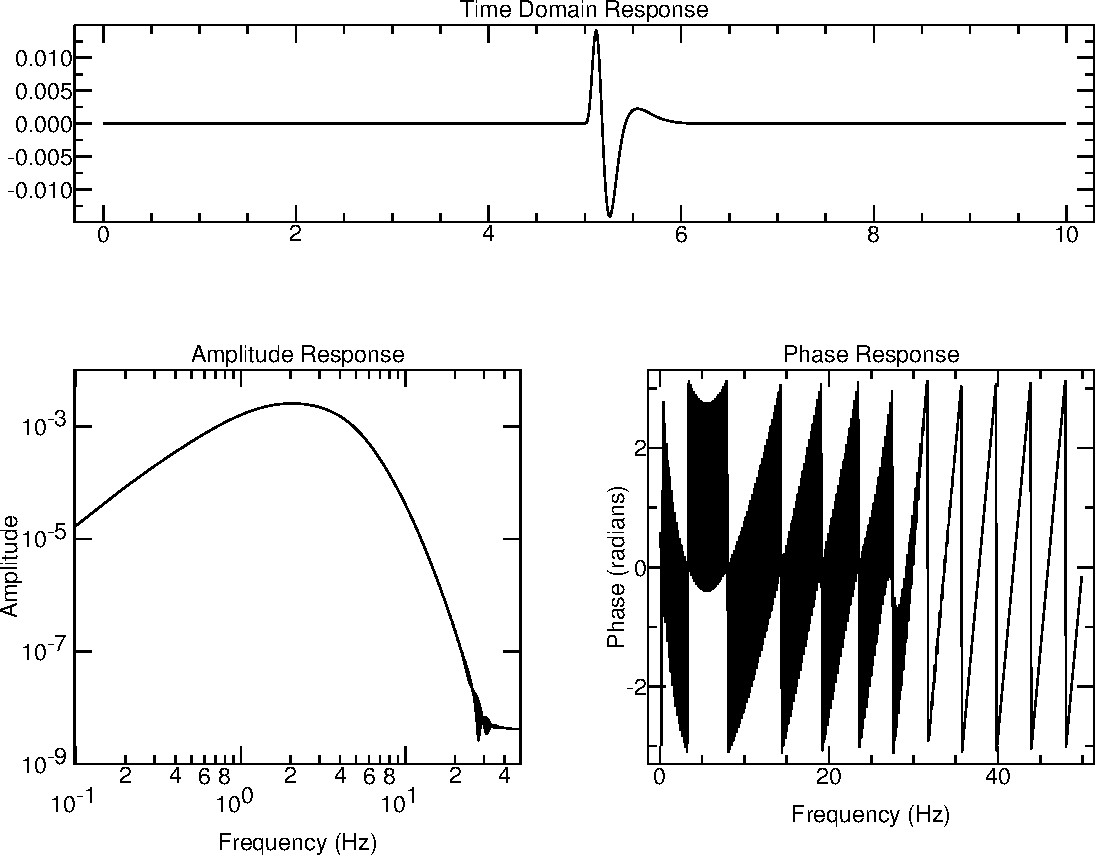
\includegraphics[width=0.8\textwidth]{benioff}
\caption{Benioff滤波器的响应函数}
\label{fig:benioff}
\end{figure}

\SACTitle{头段变量}
depmin、depmax、depmen

\SACCMD{binoperr}
\label{cmd:binoperr}

\SACTitle{概要}
控制二元操作addf、subf、mulf、divf中的错误

\SACTitle{语法}
\begin{SACSTX}
BINOPERR [N!PTS! F!ATAL!|W!ARNING!|I!GNORE!] [D!ELTA! F!ATAL!|W!ARNING!|I!GNORE!]
\end{SACSTX}

\SACTitle{输入}
\begin{description}
\item [NPTS]  改变数据点数不相等的错误条件
\item [DELTA] 改变采样周期不相等的错误条件
\item [FATAL] 设置错误条件为``致命''
\item [WARNING] 设置错误条件为``警告''
\item [IGNORE]  设置错误条件为``忽略''
\end{description}

\SACTitle{缺省值}
\begin{SACDFT}
binoperr npts fatal delta fatal
\end{SACDFT}

\SACTitle{说明}
对文件执行二元操作(addf、divf等)时,SAC会检测两个文件的数据点数和采样周期是否匹配。

使用这个命令,你可以控制SAC在遇到不匹配时如何处理。
\begin{itemize}
\item 如果设置错误条件为致命,
那么SAC在遇到错误时将停止执行当前命令,忽略当前行的其它剩余命令,输出错误信息到终端
并将控制权交还给用户。
\item 如果设置错误条件为警告,则遇到错误时会发送一个警告消息,程序
内部尽可能纠正错误并继续执行。
\item 如果设置错误条件为忽略,则SAC会纠正错误并继续而不告诉你发生了什么。
\end{itemize}

若要操作的两个数据文件的数据点数不匹配,SAC会使用数据点最少的那个文件的数据点数
作为最终结果文件的数据点数,以保证正常操作。

若要操作的两个文件采样周期不匹配,则SAC会使用第一个数据文件的采样周期作为结果文件的采样周期。

\SACTitle{示例}
假定file1有1000个数据点,file2有950个数据点:
\begin{SACCode}
SAC> binoperr npts fatal
SAC> read file1
SAC> addf file2
ERROR:  Header field mismatch: NPTS file1 file2
\end{SACCode}

上例中由于数据点数不匹配导致文件加法未执行,假设你输入:
\begin{SACCode}
SAC> binoperr npts warning
SAC> addf file2
WARNING:  Header field mismatch: NPTS file1 file2
\end{SACCode}
则仅对文件的前950个数据点执行加法操作。

\SACTitle{相关命令}
\nameref{cmd:addf}、\nameref{cmd:subf}、\nameref{cmd:mulf}、\nameref{cmd:divf}

\SACCMD{border}
\label{cmd:border}

\SACTitle{概要}
控制图形四周边框的绘制

\SACTitle{语法}
\begin{SACSTX}
BORDER [ON|OFF]
\end{SACSTX}

\SACTitle{输入}
\begin{description}
\item [ON] 打开边界绘图
\item [OFF] 关闭边界绘图 
\end{description}

\SACTitle{缺省值}
\begin{SACDFT}
border off
\end{SACDFT}

\SACTitle{说明}
参考 ``\nameref{sec:plot-appearance}''一节。

\SACTitle{相关命令}
\nameref{cmd:xvport}、\nameref{cmd:yvport}、\nameref{cmd:axes}、\nameref{cmd:ticks}

\SACCMD{capf}
\label{cmd:capf}

\SACTitle{概要}
关闭目前打开的字符数字型震相拾取文件

\SACTitle{语法}
\begin{SACSTX}
CAPF
\end{SACSTX}

\SACCMD{chnhdr}
\label{cmd:chnhdr}

\SACTitle{概要}
修改指定的头段变量的值

\SACTitle{语法}
\begin{SACSTX}
C!HN!H!DR! [FILE n1 n2 ...] field v [field v ...] [ALLT v]
\end{SACSTX}

\SACTitle{输入}
\begin{description}
\item [FILE n1 n2] 只修改内存中的指定文件的头段变量,n为内存中文件的文件号
\item [field v] SAC头段变量名及其值\footnote{为了保证数据内部一致性,以下头段变量的值
    不可用该命令修改:nvhdr、npts、nwfid、norid和nevid}
\item [ALLT v] 将所有已定义的时间相关头段变量的值加v秒,同时将参考时刻减去v秒
\end{description}

\SACTitle{说明}
关于值v的说明:
\begin{itemize}
\item 头段变量的类型和值的类型必须匹配;
\item 对于有内部空格的字符串要用单引号括起来;
\item 逻辑型头段变量的取值为TRUE或FALSE,YES或NO也可以接受;
\item 对于相对时间头段变量(B、E、O、A、F、Tn),v可以是相对参考时刻的时间偏移量(浮点型),
    也可以使用绝对时刻的形式 \texttt{GMT v1 v2 v3 v4 v5 v6},其中v1、v2、v3、v4、
    v5、v6是GMT年、一年的第一天、时、分、秒、毫秒。如果v1是两位整数,SAC假定其为当前世纪,
    除非那个时间是未来时间,那种情况下SAC假定是上个世纪,最好还是用4位整数表示年。
\item 对于任意类型的头段变量,均可以设置其值为 \texttt{undef},使头段变量未定义
\end{itemize}

该命令允许你修改指定的一个或多个文件的头段变量值。在未指定文件号的情况下,则对内
存中的所有文件进行操作。要将内存中修改后的头段覆盖磁盘文件的头段,需要使用write或
writehdr命令,SAC会对新值做有效性检查,不过你可以使用listhdr自己检查。

头段中用6个变量定义了参考时刻,这是SAC中唯一的绝对时刻,其它时刻都被转换成相对
于参考时刻的相对时间。可以使用``ALLT v''修改参考时刻以及相对时间。
参考时间被减去了v秒,相对时间被加上了v秒,
这保证了数据的绝对时刻不发生改变。为了方便,你可以通过输入绝对时刻
而非相对时间来改变时间偏移变量的值。绝对时刻首先被转换为相对时间,然后再存入头段中。

\SACTitle{示例}
为了定义内存中所有文件的事件经纬度、事件名:
\begin{SACCode}
SAC> ch evla 34.3 evlo -118.5
SAC> ch kevnm 'LA goes under'
\end{SACCode}

为了定义第二、四个文件的事件经纬度、事件名:
\begin{SACCode}
SAC> ch file 2 4 EVLA 34.3 EVLO -118.5
SAC> ch file 2 4 KEVNM 'LA goes under'
\end{SACCode}

设定初动到时为无定义状态:
\begin{SACCode}
SAC> ch a undef
\end{SACCode}

假设你知道事件的GMT起始时间,你想要快速改变头段中所有的时间变量,使得发震时刻是0
即参考时间为发震时刻,并且所有的相对时间根据这个时间去纠正相对值。

首先用GMT选项设置事件起始时间:
\begin{SACCode}
SAC> ch o GMT 1982 123 13 37 10 103
\end{SACCode}
现在使用listhdr检查发震时刻o相对于当前参考时间的描述:
\begin{SACCode}
SAC> lh o
 o = 123.103
\end{SACCode}
现在使用ALLT选项从所有的偏移时间中减去这个值,并加到参考时间上,你同时需要改变描述参考时间类型的字段:
\begin{SACCode}
SAC> ch allt -123.103 iztype iO
\end{SACCode}
注意这里的负号意味着从偏移时间中减去这个值。

更方便的做法是直接引用头段变量的值:
\begin{SACCode}
SAC> ch allt (0 - &1,o&) iztype IO
\end{SACCode}

\SACTitle{相关命令}
\nameref{cmd:listhdr}、\nameref{cmd:write}、\nameref{cmd:writehdr}

\SACCMD{chpf}
\label{cmd:chpf}

\SACTitle{概要}
关闭当前打开的HYPO震相拾取文件

\SACTitle{语法}
\begin{SACSTX}
CHPF
\end{SACSTX}

\SACTitle{说明}
自动附加指令card ``10''到被关闭的文件的结尾。

\SACCMD{color}
\label{cmd:color}

\SACTitle{概要}
控制彩色图形设备的颜色选项

\SACTitle{语法}
\begin{SACSTX}
COL!OR! [ON|OFF|color] [I!NCREMENT! [ON|OFF]] [S!KELETON! color]
    [B!ACKGROUND! color] [L!IST! S!TANDARD!|colorlist]
\end{SACSTX}
color是下面中的一个:
\begin{SACSTX}
W!HITE!|R!ED!|G!REEN!|Y!ELLOW!|BLU!E!|M!AGENTA!|C!YAN!|BLA!CK!
\end{SACSTX}

这里有些参数在缩写的情况下可能会有歧义,请谨慎使用,而且LIST选项必须放在命令的最后

\SACTitle{输入}
\begin{description}
\item [ON] 打开颜色选项单数不改变其他选项
\item [OFF] 关闭颜色选项
\item [color] 打开颜色选项并将数据设置为颜色color
\item [INCREMENT ON] 每个数据文件绘出后,根据colorlist的顺序改变颜色
\item [INCREMENT OFF] 不改变数据颜色
\item [SKELETON colo]: 按照标准颜色名或颜色号修改边框颜色
\item [BACKGROUND color] 修改背景色为color
        \footnote{白色背景与黑色线条对比强烈,可以考虑设置背景色为cyan}
\item [LIST colorlist] 改变颜色列表,将数据颜色设置为列表中第一个颜色,并打开颜色开关
\item [LIST STANDARD] 将颜色列表设为标准列表,将数据颜色设置为列表中第一个颜色,并打开颜色开关
\end{description}

\SACTitle{缺省值}
\begin{SACDFT}
color black increment off skeleton black background white
    list standard
\end{SACDFT}

\SACTitle{说明}
该命令控制设备的颜色属性,数据颜色是用于绘制这个数据文件的颜色。当一个数据文件绘制
完毕后,数据颜色可以根据颜色列表自动改变。skeleton颜色是用于绘制注释轴、标题、网格 、
框架的颜色。背景色是空框架在未绘制任何图形之前的颜色。

多数情况下你会选择标准颜色名,比如red,这是与图形设备无关的。然而有时候你可能想选择一个
非标准颜色,比如aquamarine,这个可以将颜色表装入图形设备来实现。

这个表将特定的颜色、亮度、对比度等与一个数字联系起来,然后你就可以通过设定对应的整数值
选择aquamarine作为你的绘图的一个部分的颜色,这个需要点工作量,可是如果你喜欢,这就值得。

如果你正在同一张图上绘制多个数据文件,通过INCRMENT选项可以使得不同数据有不同的颜色。
标准颜色表顺序如下:
\begin{minted}{console}
RED, GREEN, BLUE, YELLOW, CYAN, MAGENTA, BLACK
\end{minted}

\SACTitle{示例}
为了使数据颜色从红色开始不断变换:
\begin{SACCode}
SAC> color red increment
\end{SACCode}

为了设置数据颜色为红色,背景白色,蓝色边框:
\begin{SACCode}
SAC> color red background white skeleton blue
\end{SACCode}

为了设置一个数据颜色不断变换,颜色列表为red、white、blue,背景色为aquamarine(!!!):
\begin{SACCode}
SAC> color red increment backgroud 47 list red white blue
\end{SACCode}
上面的例子假设aquamarine是颜色表的47号。

\input{commands/comcor}
\SACCMD{contour}
\label{cmd:contour}

\SACTitle{概要}
利用内存中的数据绘制等值线图

\SACTitle{语法}
\begin{SACSTX}
CONT!OUR! [A!SPECT! ON|OFF]
\end{SACSTX}

\SACTitle{输入}
\begin{description}
\item [ASPECT ON] 打开视图比开关。当这个开关打开时,等值线图的视口将会调整保持数据中y与x的比值
\item [ASPECT OFF] 关闭视图比开关,这时将使用整个视口。
\end{description}

\SACTitle{缺省值}
\begin{SACDFT}
contour  aspect  off
\end{SACDFT}

\SACTitle{说明}
这个命令用于绘制二维数组数据的等值线图,包括 \nameref{cmd:spectrogram}
命令的输出。这个文件
操作的SAC文件必须``XYZ''类型的(SAC头段中IFTYPE为``IXYZ'')。有些命令可以
控制数据显示的方式:
\begin{itemize}
\item \nameref{cmd:zlevels} 控制等值线的数目以及间隔
\item \nameref{cmd:zlines} 控制等值线的线型
\item \nameref{cmd:zlabels} 控制等值线标签
\item \nameref{cmd:zticks} 控制方向标记
\item \nameref{cmd:zcolors} 控制等值线颜色
\end{itemize}

根据contour选项的不同,有两种不同的绘制等值线算法。一种快速扫描方法用于既不
选择实线型也没有时标和标识的情况。另一种慢一点的方法,在绘图之前要组合
全部的线段。你可以使用快速扫描方法粗看你的数据,然后选择其他选项绘制最终
图形。

\SACTitle{示例}
参见``\nameref{sec:contour}''一节。

\SACTitle{头段变量改变}
要求:iftype (为``IXYZ''), nxsize, nysize

使用:xminimum, xmaximum, yminimum, ymaximum

\SACTitle{相关命令}
\nameref{cmd:zcolors}、\nameref{cmd:zlabels}、\nameref{cmd:zlevels}、
\nameref{cmd:zlines}、\nameref{cmd:zticks}、\nameref{cmd:spectrogram}

\SACCMD{convert}
\label{cmd:convert}

\SACTitle{概要}
实现数据文件格式的转换

\SACTitle{语法}
\begin{SACSTX}
CONV!ERT! [FROM] [format] infile [TO [format] outfile]|[OVER [format]]
\end{SACSTX}
其中format可以为 \texttt{SAC|ALPHA}

\SACTitle{输入}
\begin{description}
\item [infile] 输入文件名
\item [outfile] 输出文件名
\item [OVER] 覆盖输入文件
\item [SAC] SAC格式二进制文件
\item [ALPHA] SAC字母数字型文件
\end{description}

\SACTitle{缺省值}
\begin{SACDFT}
convert from sac infile over sac
\end{SACDFT}

\SACTitle{说明}
这个命令将单个文件从一种格式转换为另一种格式。该命令已经逐渐被read和write命令
所取代,convert命令已经不再需要,保留该命令只是为了兼容性考虑。

\input{commands/convolve}
\SACCMD{copyhdr}
\label{cmd:copyhdr}

\SACTitle{概要}
从内存中的一个文件复制头段变量给其他所有文件

\SACTitle{语法}
\begin{SACSTX}
COPYHDR [FROM name|n] hdrlist
\end{SACSTX}

\SACTitle{输入}
\begin{description}
\item [FROM name] 从内存中文件名为 \texttt{name} 的文件中复制头段变量
\item [FROM n] 从内存中第n个文件中复制头段变量
\item [hdrlist] 要复制的头段变量列表
\end{description}

\SACTitle{缺省值}
\begin{SACDFT}
copyhdr from 1
\end{SACDFT}

\SACTitle{说明}
该命令允许你从内存中的一个文件复制任意头段变量值到内存中其他所有文件,
让数据有相同的头段使得数据易于处理。

\SACTitle{示例}
假设你使用 \texttt{ppk} 命令在文件FILE1中标记了多个时间,并将其储存到
头段变量 \texttt{T3} 和 \texttt{T4} 中。为了将这些时间标记复制到到
FILE2和FILE3中:
\begin{SACCode}
SAC> r FILE1
SAC> ppk
SAC> ... use cursor to mark times T3 and T4.
SAC> r more FILE2 FILE3
SAC> copyhdr from 1 T3 T4
\end{SACCode}

假设你读取了很多文件,想要复制文件ABC中的头段变量 \texttt{evla} 和
\texttt{evlo} 到其他所有文件中去,这时使用文件名而非数字会更简单:
\begin{SACCode}
SAC> copyhdr from abc stla stlo
\end{SACCode}

\SACCMD{correlate}
\label{cmd:correlate}

\SACTitle{概要}
计算自相关和互相关函数

\SACTitle{语法}
\begin{SACSTX}
COR!RELATE! [M!ASTER! name|n] [N!UMBER! n] [L!ENGTH! ON|OFF|v] [NO!RMALIZED!]
    [T!YPE! R!ECTANGLE!|HAM!MING!|HAN!NING!|C!OSINE!|T!RIANGLE!]
\end{SACSTX}

\SACTitle{输入}
\begin{description}
\item [MASTER name|n] 通过文件名或文件号指定主文件,所有文件将与此文件做相关
\item [NUMBER n] 设置相关窗的个数
\item [LENGTH ON|OFF] 打开/关闭固定窗长选项开关
\item [LENGTH v] 打开固定窗长选项开关,并将窗长度设置为v秒
\item [NORMALIZED] 对相关结果进行归一化
\item [TYPE RECTANGLE] 给每个窗应用矩形函数,其等价于不对窗加函数
\item [TYPE HAMMING|HANNING] 对每个窗应用Hamming/Hanning函数
\item [TYPE COSINE] 对每个窗的前后10\%的数据点应用余弦函数
\item [TYPE TRIANGLE] 对每个窗应用三角函数
\end{description}

\SACTitle{缺省值}
\begin{SACDFT}
correlate master 1 number 1 length off type rectangle
\end{SACDFT}

\SACTitle{说明}
该命令允许用户指定内存中的某个信号为主信号,并将主信号与内存中的所有信号
(包括主信号自身)进行相关。主信号与自身计算得到自相关函数,与其他信号计算得到
互相关函数。

两个信号之间的互相关函数定义如下:
\[ Cor(t) = \int_{-\infty} ^\infty f^*(\tau)g(t+\tau)d\tau \]

互相关函数的计算可以在时间域或频率域完成,该命令在频率域计算信号间的相关函数。

该命令的窗特性允许你计算对多个窗计算平均相关函数,其中窗的数目以及窗函数均可以指定。
当窗特性被打开时,会将信号划分为n个固定长度的窗,计算每个窗的互相关函数,然后将所有
的互相关函数做平均、截取到与原信号相同的数据长度,并替换内存中的原始数据文件。

当窗长度(LENGTH选项)以及窗数目(NUMBER选项)超过文件中的数据点数(NPTS)时,
会自动计算窗之间的重叠。缺省情况下,此窗特性是关闭的。

使用归一化选项,会对相关函数做归一化,最终得到的结果位于$-1$到$1$之间,由此可以得到
常用的互相关系数。

\SACTitle{示例}
以内存中第三个文件为主文件计算互相关函数:
\begin{SACCode}
SAC> r file1 file2 file3
SAC> cor master 3
\end{SACCode}
也可以通过文件名来指定主文件。

假设有两个数据文件,每个包含1000个噪声数据。将数据划分为无重叠的10个窗,每个窗包含
100个数据点,且对窗应用hanning函数,并计算10个窗的平均相关函数:
\begin{SACCode}
SAC> r file1 file2
SAC> cor type hanning number 10
\end{SACCode}

为了使窗之间有20\%的混叠,可以设置窗长度为120个数据点。假设数据采样周期为0.025(即每秒40个采样点),则窗长为3秒:
\begin{SACCode}
SAC> r file1 file2
SAC> cor type hanning number 10 length 3.0
\end{SACCode}

下面的例子计算了两个数据之间的归一化互相关函数,并从中提取出了互相关系数:
\begin{SACCode}
SAC> r file1 file2
SAC> cor norm                                   // 归一化互相关
SAC> setbb cc (max &2,depmax (abs &2,depmin))   // 取互相关函数的极值
                                                // 作为互相关系数
\end{SACCode}

\SACTitle{头段变量}
depmin、depmax、depmen

\SACCMD{cut}
\label{cmd:cut}

\SACTitle{概要}
定义要读入文件中的哪部分(即数据截窗)

\SACTitle{语法}
\begin{SACSTX}
CUT [ON|OFF|pdw|SIGNAL]
\end{SACSTX}

\SACTitle{输入}
\begin{description}
\item [ON] 打开截窗选项但不改变pdw
\item [OFF] 关闭截窗选项
\item [pdw] 打开截窗选项并修改pdw。关于pdw,参考 \nameref{subsec:pdw} 一节。
\item [SIGNAL] 等效于设置pdw为``\texttt{A -1 F 1}'',即a前一秒到f后一秒的数据窗
\end{description}

\SACTitle{缺省值}
\begin{SACDFT}
cut off
\end{SACDFT}

\SACTitle{说明}
cut命令仅仅设置了要读取的时间窗选项,并不对内存中的数据进行截取。因而,若要
该命令起作用,需要在cut命令设置时间窗后使用read命令。与此相反,cutim命令会
在命令执行时直接对内存中的数据进行截取。

若截窗选项为关,则读取整个文件;若截窗选项为开,则只读取由pdw定义的部分。

如果你想对一组有不同参考时刻的文件使用同样的时间窗,必须在执行cut前先使用synchronize
命令使所有文件具有相同的参考时刻。synchronize命令修改了文件的头段使得所有文件
具有相同的参考时刻,并调整所有相对时间。因而,你需要先读取所有文件,执行synchronize
命令,使用writehdr将修改后的头段写入到磁盘文件中,然后再执行cut命令,并读取数据,
这样才能得到正确的结果。

\SACTitle{示例}
下面的宏文件展示了cut命令的一些常见用法。建议将此宏文件的结果与cutim命令的宏文件
结果进行比较:
\begin{SACCode}
fg seismo
wrie seismo.sac
echo on
* no cutting
lh b e a kztime
read seismo.sac
* begin to end---same as not cutting.
cut B E
read
lh b e a kztime
read seismo.sac
* First 3 secs of the file
cut B 0 3
read
lh b e a kztime
read seismo.sac
* First 100 points of the file.
cut B N 100
read
lh b e a delta kztime
read seismo.sac
* From 0.5 secs before to 3 secs after first arrival
cut A -0.5 3
read
lh b e a kztime
read seismo.sac
* From 19 to 15 secs relative to zero (DIFFERENT FROM CUTIM).
cut 10 15
read
lh b e a kztime
read seismo.sac
* First 3 secs of the file and next 3 sec
cut b 0 3
read
write tmp.1
read seismo.sac
cut b 3 6
read
write tmp.2
cut off
read tmp.?
lh b e a kztime
p1
\end{SACCode}

当要截取的窗超过了文件的时间范围时,可以使用CUTERR命令的FILLZ选项,
在文件的开始或结尾处补0,再使用READ命令读入内存。
\begin{SACCode}
SAC> r N11A.lhz
SAC> lh npts
FILE: N11A.lhz - 1
npts = 3101
SAC> cuterr fillz; cut b n 4096
SAC> r
SAC> lh npts
FILE: N11A.lhz - 1
npts = 4096
\end{SACCode}

\SACTitle{限制}
目前不支持非等间隔文件或谱文件的截断。该命令对ASCII格式的SAC文件无效。

\SACCMD{cuterr}
\label{cmd:cuterr}

\SACTitle{概要}
控制坏的截窗参数引起的错误

\SACTitle{语法}
\begin{SACSTX}
CUTERR FA!TAL!|U!SEBE!|FI!LLZ!
\end{SACSTX}

\SACTitle{输入}
\begin{description}
\item [FATAL] 将截窗错误设置为致命
\item [USEBE] 将坏的起始和结束截窗参数设置为文件开始和文件结束
\item [FILLZ] 在文件开始时间之前或文件结束时间之后填补适当数目的0以弥补坏的截窗参数
\end{description}

\SACTitle{缺省值}
对于信号迭加子程序默认值为FILLZ,其他的默认值为USEBE

\SACTitle{说明}
这个命令控制由于坏的截窗参数引起的错误条件。可以将这些错误定义为致命错误。
如果裁剪参数的起始值或结束值在文件头段中未定义,则可以选择为USEBE。如果
定义了要截取的时间窗但是其截窗起始值小于文件起始值或者截窗参数结束值大于
文件结束值,则可以分别用文件起始结束值代替截窗参数,或者也可以使用FILLZ
在文件前后补适当的0。

\SACTitle{示例}
假设文件FILE1起始时间为B=\SI{25}{s},初动到时A=\SI{40}{s},采样率为 \SI{0.01}{s}。
\begin{SACCode}
SAC> cut a -20 e
SAC> read file1
\end{SACCode}
截窗起始值为 \SI{20}{s},产生了一个错误条件。在USEBE模式下,截窗起始值
将替换为 \SI{25}{s}(即B)。在FILLZ模式下,在数据之前将将插入500个零值(5秒钟,
每秒100个点),截窗起始值保持为 \SI{20}{s}。

\SACCMD{cutim}
\label{cmd:cutim}

\SACTitle{概要}
截取内存中的文件\footnote{该命令似乎有问题,执行该命令时,似乎会删除内存中的全部
波形数据,请勿使用}

\SACTitle{语法}
\begin{SACSTX}
CUTIM pdw [pdw ... ]
\end{SACSTX}

\SACTitle{输入}
\begin{description}
\item [pdw] 要截取的时间窗。参考 \nameref{subsec:pdw}
\end{description}

\SACTitle{缺省值}
如果起始或结束offset省略则认为其为0,如果起始参考值省略则认为其为Z,如果结束参考值省略则认为其值与起始参考值相同。

\SACTitle{说明}
cut命令设置截窗选项,仅对即将读取的文件进行截窗,而对内存中的数据没有效果。
cutim则在这个命令给出的时候对内存中的数据进行截窗操作。

用户可以用read读入文件,然后用cutim对内存中的文件直接进行截窗。
cutim也允许使用多个截取区间,用户可以READ三个文件到内存,然后使用有4个截取区间的
CUTIM命令,最终内存中将得到12个文件。

\SACTitle{示例}
下面的宏文件展示了cutim命令的常见用法:
\begin{SACCode}
fg seismo
echo on
* no cutting
lh b e a kztime
* begin to end---same as not cutting.
cutim B E
lh b e a kztime
fg seismo
* First 3 secs of the file.
cutim B 0 3
lh b e a kztime
fg seismo
* From 0.5 secs before to 3 secs after first arrival
cutim A -0.5 3
lh b e a kztime
fg seismo
* From 0.5 to 5 secs relative to disk file start.
cutim 0.5 5
lh b e a kztime
fg seismo
* First 3 secs of the file and next 3 sec
cutim b 0 3 b 3 6
lh b e a kztime
p1
\end{SACCode}

\SACTitle{限制}
目前不支持截取非等间隔数据或谱文件

\SACTitle{相关命令}
\nameref{cmd:read}、\nameref{cmd:apk}、\nameref{cmd:plotpk}、\nameref{cmd:synchronize}、\nameref{cmd:cuterr}

\SACCMD{datagen}
\label{cmd:datagen}

\SACTitle{概要}
产生样本波形数据并储存在内存中

\SACTitle{语法}
\begin{SACSTX}
D!ATA!G!EN! [MORE] [SUB L!OCAL!|R!EGIONAL!|T!ELESEIS!] [filelist]
\end{SACSTX}

\SACTitle{输入}
\begin{description}
\item [MORE] 将新生成的样本数据放在内存中旧文件后。若省略此项,则新数据将替代内存中的旧数据。
\item [SUB LOCAL|REGIONAL|TELESEIS] 要生成的数据的子类型,每个子类型对应不同的样本数据
\item [filelist] 样本数据文件列表。每个子类型可选的文件列表在下面给出。
\end{description}

\SACTitle{缺省值}
\begin{SACDFT}
datagen sub local cdv.z
\end{SACDFT}

\SACTitle{说明}
SAC提供了一些样本地震数据以供用户学习时使用,该命令将读取一个或多个样本地震数据
到内存中。事实上,该命令与READ命令类似,只是该命令是从特殊的数据目录中读取文件。

该命令提供了三种子类型,分别是LOCAL、REGIONAL和TELESEIS,对于不同的子类型,其所
包含的数据文件也不同。

\subsubsection*{LOCAL}
该local事件发生在加州的Livermore Valley,是一个很小的无感地震(ML=1.6),其被
Livermore Local Seismic Network (LLSN)所记录。

LLSN拥有一系列垂直分量和三分量台站。该数据集中包含了9个三分量台站的数据。
数据时长40秒,每秒100个采样点。台站信息、事件信息、p波及尾波到时都包含在头段中,
这些文件包括:
\begin{SACCode}
    cal.z, cal.n, cal.e
    cao.z, cao.n, cao.e
    cda.z, cda.n, cda.e
    cdv.z, cdv.n, cdv.e
    cmn.z, cmn.n, cmn.e
    cps.z, cps.n, cps.e
    cva.z, cva.n, cva.e
    cvl.z, cvl.n, cvl.e
    cvy.z, cvy.n, cvy.e
\end{SACCode}

\subsubsection*{REGIONAL}
该区域地震发生在Nevada,被Digital Seismic Network (DSS)所记录。DSS包含了美国西部的四个宽频带三分量台站。数据包含了从发震前5秒开始的为300秒地震数据,每秒含40个采样点,文件名为:
\begin{SACCode}
    elk.z, elk.n, elk.e
    lac.z, lac.n, lac.e
    knb.z, knb.n, knb.e
    mnv.z, mnv.n, mnv.e
\end{SACCode}

\SACTitle{TELESEIS}
该远震事件于1984年9月10日发生在加州北海岸Eureka附近,其为中等偏大的地震(ML 6.6, MB 6.1, MS 6.7) ,
多地有感。该数据集中包含了Regional Seismic Test Network(RSTN)的5个台站的中等周期和长周期数据
(其中cpk台站的数据无法获取,sdk台站的长周期数据被截断)。这个数据集的数据时长1600秒,长周期
数据每秒1个采样点,中等周期数据每秒4个采样点。文件包括:
\begin{SACCode}
    ntkl.z, ntkl.n, ntkl.e, ntkm.z, ntkm.n, ntkm.e
    nykl.z, nykl.n, nykl.e, nykm.z, nykm.n, nykm.e
    onkl.z, onkl.n, onkl.e, onkm.z, onkm.n, onkm.e
    sdkl.z, sdkl.n, sdkl.e, sdkm.z, sdkm.n, sdkm.e
\end{SACCode}

\SACCMD{decimate}
\label{cmd:decimate}

\SACTitle{概要}
对数据做减采样

\SACTitle{语法}
\begin{SACSTX}
DEC!IMATE! [n] [F!ILTER! ON|OFF]
\end{SACSTX}

\SACTitle{输入}
\begin{description}
\item [n] 设置减采样因子为n,即每n个点中取一个点,n取值范围为2到7
\item [FILTER ON|OFF] 打开/关闭抗混叠FIR滤波器
\end{description}

\SACTitle{缺省值}
\begin{SACDFT}
decimate 2 filter on
\end{SACDFT}

\SACTitle{说明}
此命令用于对内存中的数据进行减采样,减采样因子n表示从每n个数据点中取
一个点,因而经过减采样之后的数据点数近似为$npts/n$个。减采样因子的允许
取值为2到7,为了得到更大的减采样因子,可以多次执行该命令。

根据采样定理:
\begin{quote}
如果信号是带限的,并且采样频率大于信号带宽的2倍,那么,原来的连续信号
可以从采样样本中完全重建出来。
\end{quote}
若不满足此采样条件,采样后信号的频率就会重叠,即高于采样频率一半的频率
成分将被重建成低于采样频率一半的信号。这种频谱重叠导致的失真称为混淆
效应。

该命令提供了一个可选的FIR滤波器对数据进行低通滤波,以避免减采样过程中
可能出现的混淆效应。可用的的FIR滤波器的具体参数位于 \verb|$SACHOME/aux/fir/decn|
中,这些滤波器是经过精心设计的,保留了相位信息。使用FIR滤波器有时会在
数据的两端产生瞬时跳变,因而减采样的结果需要在图形界面下人工审核。只有
当高频响应的准确度不重要的时候(比如绘图时),才可以关闭FIR滤波器。

\SACTitle{示例}
对数据减采样42倍:
\begin{SACCode}
SAC> r file1
SAC> decimate 7     // 减采样因子为7时FIR滤波器偶尔不稳定,慎用!
SAC> decimate 6
\end{SACCode}

\SACTitle{头段变量}
npts、delta、e、depmin、depmax、depmen

\SACCMD{deletechannel}
\label{cmd:deletechannel}

\SACTitle{概要}
从内存文件列表中删去一个或多个文件

\SACTitle{语法}
\begin{SACSTX}
D!ELETE!C!HANNEL! ALL
\end{SACSTX}
或
\begin{SACSTX}
D!ELETE!C!HANNEL! fname|filenumber|range [fname|filenumber|range ...]
\end{SACSTX}

\SACTitle{输入}
\begin{description}
\item [ALL] 删除内存中全部文件
\item [fname] 要删除的内存文件列表中的文件名
\item [filenumber] 文件列表中指定文件的文件号,第一个文件是1,第二个文件是2...
\item [range] 要删除的一系列文件号,用破折号隔开,如11-20
\end{description}

\SACTitle{示例}
\begin{SACCode}
  dc 3 5                         // 删除第三、五个文件
  dc SO01.sz SO02.sz             // 删除这些名字的文件
  dc 11-20                       // 删除11-20的全部文件
  dc 3 5 11-20 SO01.sz SO02.sz   // 删除上面的全部
\end{SACCode}

\SACCMD{dif}
\label{cmd:dif}

\SACTitle{概要}
对数据进行微分

\SACTitle{语法}
\begin{SACSTX}
DIF [TW!O!|TH!REE!|F!IVE!]
\end{SACSTX}

\SACTitle{输入}
\begin{description}
\item [TWO]   使用两点差分算子
\item [THREE] 使用三点差分算子
\item [FIVE]  使用五点差分算子
\end{description}

\SACTitle{缺省值}
\begin{SACDFT}
dif two
\end{SACDFT}

\SACTitle{说明}
该命令通过对数据应用差分算法实现数据的微分操作,要求数据必须是等间隔采样的时间序列文件。
微分会使位移量变成速度量,速度量变成加速度量,因而微分的同时会修改头段变量 
\texttt{idep} 的值。

两点差分算法:
\[ Out(j) =\frac{Data(j+1) - Data(j)}{\Delta} \]
两点差分算子不是中心差分算法。此算法的最后一个输出值是未定义的,SAC的处理方式是:
令数据点数减1,文件起始时间 \texttt{B} 增加半个采样周期。

三点(中心两点)差分算法:
\[ Out(j) = \frac{1}{2} \frac{Data(j+1) - Data(j-1)}{\Delta} \]
此算法输出值的第一个和最后一个是未定义的,SAC将数据点数减去2,并将文件起始时间 \texttt{B}
增加一个采样周期。

五点(中心四点)差分算法:
\[ Out(j) = \frac{2}{3} \frac{Data(j+1) - Data(j-1)}{\Delta} - \frac{1}{12} \frac{Data(j+2) - Data(j-2)}{\Delta} \]
此算法输出值的首尾各两个点是未定义的,SAC使用三点差分算符计算第二个和倒数第二个点
的值,并将数据点数减2,将 \texttt{B} 增加一个采样周期。



\SACTitle{头段变量改变}
npts、b、e、depmin、depmax、depmen、idep

\SACCMD{div}
\label{cmd:div}

\SACTitle{概要}
数据文件的每个数据点除以同一个常数

\SACTitle{语法}
\begin{SACSTX}
DIV [v1 [v2 ... vn] ]
\end{SACSTX}

\SACTitle{输入}
\begin{description}
\item [v1] 第一个文件要除以的常数
\item [v2] 第二个文件要除以的常数
\item [vn] 第n个文件要除以的常数
\end{description}

\SACTitle{缺省值}
\begin{SACDFT}
div 1.0
\end{SACDFT}

\SACTitle{说明}
参见 \nameref{cmd:add} 的相关说明。

\SACTitle{头段变量改变}
depmin、depmax、depmen

\SACCMD{divf}
\label{cmd:divf}

\SACTitle{概要}
使内存中的一组数据除以另一组数据

\SACTitle{语法}
\begin{SACSTX}
DIVF [NEWHDR [ON|OFF]] filelist
\end{SACSTX}

\SACTitle{输入}
\begin{description}
\item [NEWHDR ON|OFF] 指定新生成的文件使用哪个文件的头段。\texttt{OFF}
    表示使用内存中原文件的头段区,\texttt{ON} 表示使用filelist中文件的
    头段区。缺省值为 \texttt{OFF}
\item [filelist] SAC二进制文件列表
\end{description}

\SACTitle{说明}
参见 \nameref{cmd:addf} 命令的相关说明。

\SACTitle{头段变量}
depmin、depmax、depmen、npts、delta

\SACCMD{divomega}
\label{cmd:divomega}

\SACTitle{概要}
在频率域进行积分操作

\SACTitle{语法}
\begin{SACSTX}
DIVOMEGA
\end{SACSTX}

\SACTitle{说明}
根据傅里叶变换的微分性质:
\[
\mathcal{F}[f'(x)]= i \omega \mathcal{F}[f(x)]
\]
其中$\omega = 2 \pi f $,即函数积分在频率域可以用简单的除法来表示。

该命令仅可对谱文件进行操作,谱文件可以是振幅-相位型或实部-虚部型。
对于正常的谱数据来说还是很方便的,但不适用于谱跨越几个量级的数据。
比如,假设你使用 \texttt{dif} 命令对数据进行预白化,然后对数据进行
Fourier变换,用此命令在频率域积分可以去除时间域微分的效应。

若为振幅-相位型:
\[
\mathcal{F}[f(x)] = \frac{\mathcal{F}[f'(x)]}{i \omega}
                  = \frac{A(\omega)e^{\theta(\omega)}}{i \omega}
                  = \frac{A(\omega)}{\omega}e^{\theta(\omega)-\pi/2}
\]

若为实部-虚部型:
\[
\mathcal{F}[f(x)] = \frac{\mathcal{F}[f'(x)]}{i \omega}
                  = \frac{a(\omega)+ib(\omega)}{i \omega}
                  = \frac{b(\omega)}{\omega}-i\frac{a(\omega)}{\omega}
\]

在零频部分,直接设置其值为0比避免除以0的问题。

\SACTitle{示例}
\begin{SACCode}
SAC> read file1
SAC> dif                // 微分预白化
SAC> fft amph           // FFT
SAC> divomega           // 积分
\end{SACCode}

\SACTitle{头段变量}
depmin、depmax、depmen

\SACCMD{echo}
\label{cmd:echo}

\SACTitle{概要}
控制输入输出回显到终端

\SACTitle{语法}
\begin{SACSTX}
ECHO ON|OFF E!RRORS!|W!ARNINGS!|O!UTPUT!|C!OMMANDS!|M!ACROS!|P!ROCESS!
\end{SACSTX}

\SACTitle{输入}
\begin{description}
\item [ON|OFF] 打开/关闭列出的项的回显选项
\item [ERRORS] 命令执行过程中生成的错误信息
\item [WARNINGS] 命令执行过程中生成的警告信息
\item [OUTPUT] 命令执行过程中生成的输出信息
\item [COMMANDS] 终端键入的原始命令
\item [MACROS] 宏文件中出现的原始命令
\item [PROCESSED] 经过处理后的终端命令或宏文件命令,包括宏参数、黑板
    变量、头段变量、内联函数的计算和代入
\end{description}

\SACTitle{缺省值}
\begin{SACDFT}
echo on errors warnings output off commands macros processed
\end{SACDFT}

\SACTitle{说明}
该命令控制SAC输入输出流中哪一类要被回显到终端或屏幕。

输出分为三大类:错误消息、警告消息、输出消息;输入也分为三大类:终端键入
的命令、宏文件中执行的命令以及处理后的命令。处理后的命令指所有的宏参数、
黑板变量、头段变量、内联函数首先被计算,并代入到命令中而形成的命令。
你可以分别控制这些类的回显。

当在终端键入命令时,操作系统一般会显示用户键入的每个字符,因此该命令
在交互式会话中没有太大作用。设置显示宏命令以及处理后的命令在调试宏文件
时会很有用。

\SACCMD{enddevices}
\label{cmd:enddevices}

\SACTitle{概要}
结束某个图像设备

\SACTitle{语法}
\begin{SACSTX}
E!ND!D!EVICES! S!GF!|X!WINDOWS!
\end{SACSTX}

\SACTitle{输入}
\begin{description}
\item [SGF] SAC图形文件设备
\item [XWINDOWS] X Window System图像窗口系统
\end{description}

\SACTitle{说明}
参见命令 \nameref{cmd:begindevices} 的说明。

\SACTitle{相关命令}
\nameref{cmd:begindevices}

\SACCMD{endframe}
\label{cmd:endframe}

\SACTitle{概要}
关闭frame

\SACTitle{语法}
\begin{SACSTX}
E!ND!F!RAME!
\end{SACSTX}

\SACTitle{说明}
参见 \nameref{cmd:beginframe} 命令的相关说明。

\SACTitle{相关命令}
\nameref{cmd:beginframe}

\SACCMD{envelope}
\label{cmd:envelope}

\SACTitle{概要}
利用Hilbert变换计算包络函数

\SACTitle{语法}
\begin{SACSTX}
ENVELOPE
\end{SACSTX}

\SACTitle{说明}
该命令用于计算内存中数据的包络函数。

原始信号为$s(t)$,对其做Hilbert变换得到$H(t)$,将这两个信号合并起来构成复信号
\[
    C(t) = s(t) + i*H(t)
\]

复信号不仅可以用``实部-虚部''形式表示,也可以用``振幅-相位''形式表示:

\[
    C(t) = A(t) e^{i\Phi(t)}
\]

其中$A(t)$即为包络函数,其可以进一步表示为
\[
    A(t) = \sqrt{s(t)^2+H(t)^2}
\]

和 \nameref{cmd:hilbert} 一样,数据点数不得少于201,且超长周期的数据需要
在处理之前进行减采样。

\SACTitle{头段变量}
depmin、depmax、depmen

\SACTitle{相关命令}
\nameref{cmd:hilbert}、\nameref{cmd:decimate}

\input{commands/erase}
\SACCMD{evaluate}
\label{cmd:evaluate}

\SACTitle{概要}
对简单算术表达式求值

\SACTitle{语法}
\begin{SACSTX}
EVAL!UATE! [TO TERM|name] [v] op v [op v ...]
\end{SACSTX}
其中op为下面中的一个:
\begin{SACSTX}
ADD|SUBTRACT|MULTIPLY|DIVIDE|POWER|SQRT|EXP|ALOG|ALOG10|
SIN|ASIN|COS|ACOS|TAN|ATAN|EQ|NE|LE|GE|LT|GT
\end{SACSTX}

\SACTitle{输入}
\begin{description}
\item [TO TERM] 结果写入终端
\item [TO name] 结果写入黑板变量name
\item [v] 浮点数或整数。SAC中所有的运算都是浮点运算,整数会首先转换为浮点型
\item [op] 算术或逻辑操作符
\end{description}

\SACTitle{其他形式}
\begin{itemize}
\item \texttt{+} 代替ADD
\item \texttt{-} 代替SUBTRACT
\item \texttt{*} 代替MULTIPLY
\item \texttt{/} 代替DIVIDE
\item \texttt{**} 代替POWER
\end{itemize}

\SACTitle{缺省值}
\begin{SACDFT}
evaluate to term 1. * 1.
\end{SACDFT}

\SACTitle{说明}
这个命令允许你对算术或逻辑表达式求值。算术表达式可以是包含多个操作符的复合表达式,
在这种情况下表达式由左向右计算,不支持嵌套功能。逻辑表达式只能包含一个操作符。
计算结果可以写入用户终端或者指定的黑板变量。你可以通过getbb命令使用该黑板变量的值。

\SACTitle{示例}
一个简单的例子:
\begin{SACCode}
SAC> eval 2*3
 6
SAC> eval tan 45
1.61978
\end{SACCode}

下面将一个以度为单位的角度转换为弧度并计算其正切值:
\begin{SACCode}
SAC> eval 45*pi/180
 0.785398
SAC> eval tan 0.785398
 1
\end{SACCode}

下面将计算的结果保存到黑板变量:
\begin{SACCode}
SAC> evaluate to temp1 45*pi/180
SAC> evaluate tan %temp1%
 1
\end{SACCode}

\SACTitle{相关命令}
\nameref{cmd:getbb}

\SACCMD{exp}
\label{cmd:exp}

\SACTitle{概要}
对每个数据点取其指数($e^y$)

\SACTitle{语法}
\begin{SACSTX}
EXP
\end{SACSTX}

\SACTitle{头段变量}
depmin、depmax、depmen

\SACCMD{exp10}
\label{cmd:exp10}

\SACTitle{概要}
对每个数据点取以10为底的指数($10^y$)

\SACTitle{语法}
\begin{SACSTX}
EXP10
\end{SACSTX}

\SACTitle{头段变量}
depmin、depmax、depmen

\SACCMD{fft}
\label{cmd:fft}

\SACTitle{概要}
对数据做快速离散傅立叶变换

\SACTitle{语法}
\begin{SACSTX}
FFT [WO!MEAN!|W!MEAN!] [R!LIM!|A!MPH!]
\end{SACSTX}

\SACTitle{输入}
\begin{description}
\item [WOMEAN] 变换前先去除均值
\item [WMEAN] 变换前不去除均值
\item [RLIM] 输出为实部-虚部格式
\item [AMPH] 输出为振幅-相位格式
\end{description}

\SACTitle{缺省值}
\begin{SACDFT}
fft wmean amph
\end{SACDFT}

\SACTitle{说明}
该命令对数据进行离散傅立叶变换。为了使用快速傅立叶变换算法,在进行变换
之前,需要对数据文件进行补零以保证数据点数为2的整数次幂,比如1000个点的
时间序列文件会被补零至1024个点,且头段变量 \texttt{npts} 也会被相应修改。

进行离散傅立叶变换之后,头段变量 \texttt{b} 为谱文件的起始频率,其值为0;
\texttt{delta} 为谱文件的采样频率,取值为 \texttt{1/(delta*npts)};
\texttt{e} 为谱文件的结束频率。\texttt{b}、\texttt{e}、\texttt{npts} 和
\texttt{delta} 的原值被保存到 \texttt{sb}、\texttt{se}、\texttt{nsnpts}
和 \texttt{sdelta},这些值在做反傅立叶变换时会用到。

傅里叶变换得到的谱数据可以是振幅-相位格式或实部-虚部格式。头段变量
\texttt{iftype} 会告诉你谱文件是哪种格式。

由于实序列的离散傅立叶变换的结果具有``共轭对称性'',因而在使用
\nameref{cmd:plotsp} 绘制谱文件时只显示一半的数据点数。

\SACTitle{示例}
\begin{SACCode}
SAC> fg seis
SAC> lh b e delta npts iftype

          b = 9.459999e+00
          e = 1.945000e+01
      delta = 1.000000e-02
       npts = 1000
     iftype = TIME SERIES FILE
SAC> fft
 DC level after DFT is -0.98547
SAC> lh b e delta npts iftype

          b = 0.000000e+00              // b值为0
          e = 5.000000e+01
      delta = 9.765625e-02              // delta=1/(1024*0.01)
       npts = 1024                      // 1000 -> 1024
     iftype = SPECTRAL FILE-AMPL/PHASE
SAC> lh sb sdelta nsnpts                // 保留原值

         sb = 9.459999e+00
     sdelta = 1.000000e-02
     nsnpts = 1000
\end{SACCode}

\SACTitle{头段变量}
b、e、delta、npts、sb、se、nsnpts、sdelta

\SACTitle{限制}
离散傅立叶变换所允许的最大数据点数为$2^{24}=16777216$个。

\SACCMD{fileid}
\label{cmd:fileid}

\SACTitle{概要}
控制绘图时文件ID的显示

\SACTitle{语法}
\begin{SACSTX}
FILEID [ON|OFF] [T!YPE! D!EFAULT!|N!AME!|L!IST! hdrlist]
    [L!OCATION! UR|UL|LR|LL] [F!ORMAT! E!QUALS!|C!OLONS!|N!ONAMES!]
\end{SACSTX}

\SACTitle{输入}
\begin{description}
\item [ON] 显示文件id,不改变文件id类型或位置
\item [OFF] 不显示文件id
\item [TYPE DEFAULT] 设置文件id为默认类型
\item [TYPE NAME] 使用文件名作为文件id
\item [TYPE LIST hdrlist] 定义在文件id中显示的头段列表
\item [LOCATION UR|UL|LR|LL] 文件id的显示位置,分别表示右上角、左上角、
    右下角、左下角
\item [FORMAT EQUALS] 格式为 \texttt{variable=value}
\item [FORMAT COLON] 格式为 \texttt{variable:value}
\item [FORMAT NONAMES] 格式只包含头段值
\end{description}

\SACTitle{缺省值}
\begin{SACDFT}
fileid on type default location ur format nonames
\end{SACDFT}

\SACTitle{说明}
文件ID用于标识绘图的内容。默认的文件ID包括事件名、台站名、分量、参考
日期及时间。如果需要也可以使用文件名代替默认的文件id,或者根据头段变量
定义一个特殊的文件ID,这个ID最多可以由10个SAC头段变量构成。文件ID的位置
以及格式也可以修改。

\SACTitle{示例}
将文件名放在左上角:
\begin{SACCode}
SAC> fileid location ul type name
\end{SACCode}

定义一个特殊的文件id,包含台站分量、经纬度:
\begin{SACCode}
SAC> fileid type list kstcmp stla stlo
\end{SACCode}

文件id为头段名后加一个冒号:
\begin{SACCode}
SAC> fileid format colon
\end{SACCode}

\SACCMD{filenumber}
\label{cmd:filenumber}

\SACTitle{概要}
控制绘图时文件号的显示

\SACTitle{语法}
\begin{SACSTX}
F!ILE!N!UMBER! [ON|OFF]
\end{SACSTX}

\SACTitle{缺省值}
\begin{SACDFT}
filenumber off
\end{SACDFT}

\SACTitle{说明}
当该选项为开时,绘图时会在右下角显示文件号,当需要文件号的信息时可以
通过此文件号唯一识别指定的波形。

\SACCMD{filterdesign}
\label{cmd:filterdesign}

\SACTitle{概要}
产生一个滤波器的数字和模拟特性的图形显示,包括:振幅,相位,脉冲响应和群延迟。

\SACTitle{语法}
\begin{SACSTX}
F!ILTER!D!ESIGN! [FILE [prefix]] [filteroptions] [delta]
\end{SACSTX}
其中filteroptions与SAC中其他的滤波命令相同,包括滤波器类型。delta是数据的采样间隔。

注意:选项的顺序很重要,如果使用了PRINT选项,则其必须是第一个选项。如果使用了FILE选项,其必须放在滤波器选项之前。

\SACTitle{输入}
\begin{description}
\item [FILE prefix] 生成的三个SAC文件的前缀
\end{description}

这三个SAC文件分别为prefix.spec、prefix.grd、prefix.imp。其中prefix.spec为
该命令产生的振幅相位信息,为振幅-相位格式谱文件。prefix.gd为该命令产生的群延迟信息,
是时间序列文件。需要注意的是,尽管这个文件是时间序列文件,但是实际上群延迟是频率的函数。
用户要记住,虽然绘图时横轴单位是秒,实际的单位却是 \si{\Hz}。prefix.imp是时间序列文件,
包含脉冲响应信息。

在这三个SAC文件中,用户自定义头段变量USERn、KUSERn设置如下:
\begin{itemize}
\item user0:表示pass code。1代表LP;2代表HP;3代表BP;4代表BR;
\item user1:type code。1代表BU,2代表BE,3代表C1,4代表C2;
\item user2:number of poles
\item user3:number of passes
\item user4:tranbw
\item user5:attenuation
\item user6:delta
\item user7:first corner
\item user8:second corner if present, or -12345 if not
\item kuser0:pass (lowpass, highpass, bandpass, or bandrej)
\item kuser1:type (Butter, Bessel, C1, or C2 )
\end{itemize}

\SACTitle{缺省值}
只有delta参数有一个缺省值(\SI{0.025}{\s})。其他参数必须给出

\SACTitle{说明}
FILTERDESIGN命令使用了一个工具程序xapiir,它是一个递归数字滤波器包。
xapiir通过模拟滤波器原型的双线性变换实现标准递归数字滤波器的设计。
这些原型滤波器由零点和极点给定,然后使用模拟谱变换,变换到高通、带通和带阻滤波器。

FILTERDESIGN用实线显示数字滤波器响应,用虚线显示模拟滤波器响应。
在彩色显示器上,数字曲线是蓝色的而模拟曲线是琥珀色的。

\SACTitle{示例}
下面的例子展示了如何使用FILTERDESIGN命令产生一个高通,拐角频率为 \SI{2}{\Hz},
六极、双通滤波器的数字和模拟响应曲线,数据采样间隔为 \SI{0.025}{\s}:
\begin{SACCode}
SAC> fd hp c 2 n 6 p 2 delta .025
\end{SACCode}

\SACTitle{相关命令}
\nameref{cmd:highpass}、\nameref{cmd:lowpass}、\nameref{cmd:bandpass}、\nameref{cmd:bandrej}

\SACCMD{fir}
\label{cmd:fir}

\SACTitle{概要}
应用一个有限脉冲响应滤波器

\SACTitle{语法}
\begin{SACSTX}
FIR [REC|FFT] file
\end{SACSTX}

\SACTitle{输入}
\begin{description}
\item [FFT] 通过FFT变换方法应用FIR滤波器
\item [REC] 递归应用FIR滤波器
\item [file] 包含FIR滤波器的文件名
\end{description}

\SACTitle{缺省值}
\begin{SACDFT}
fir fft fir
\end{SACDFT}

\SACTitle{说明}
这个命令中使用的滤波器必须首先用DFIR交互式滤波器设计。这个滤波器通过变换方法应用,除非你要求使用递归方法或者数据点数对于变换方法来说太大。这些滤波器都没有相位失真但在脉冲信号前会产生前驱波。

\SACTitle{头段变量}
depmin、depmax、depmen

\SACTitle{限制}
变换方法的最大数据点数是4096。

\input{commands/floor}
\SACCMD{funcgen}
\label{cmd:funcgen}

\SACTitle{概要}
生成一个函数并将其存在内存中

\SACTitle{语法}
\begin{SACSTX}
F!UNC!G!EN! [type] [D!ELTA! v] [N!PTS! n] [BE!GIN! v]
\end{SACSTX}
其中type是下面中的一个:
\begin{SACSTX}
IMP!ULSE! | ST!EP! | B!OXCAR! | T!RIANGLE! | SINE [v1 v2] | L!INE! [v1 v2] |
Q!UADRATIC! [v1 v2 v3] | CUBIC [v1 v2 v3 v4] | SEIS!MOGRAM! |
R!ANDOM! [v1 v2] | IMPSTRIN  [n1 n2 ... nN]
\end{SACSTX}

\SACTitle{输入}
\begin{description}
\item [IMPULSE] 位于数据中心的脉冲函数
\item [IMPSTRIN n1 n2 ... nN] 在指定的一系列数据点处产生脉冲函数
\item [STEP] 阶跃函数。数据的前半段为0,后半段为1
\item [BOXCAR] 矩形函数。数据的前、后三分之一值为0,中间三分之一值为1
\item [TRIANGLE] 三角函数。数据的第一个四分之一为0,第二个四分之一线性增加到1,第三个四分之一
    线性减少到0,最后四分之一为0。
\item [SINE v1 v2] 正弦函数。v1表示频率,单位为 \si{\Hz};v2为以度为单位的相位角。正弦函数的振幅为1,
    注意在相位参数中有一个$2\pi$因子: $F = 1.0 \sin (2\pi (v_1t+v_2))$
\item [LINE v1 v2] 线性函数。斜率为v1,截距为v2,即$ v_1 t + v_2 $
\item [QUADRATIC v1 v2 v3] 二次函数 $v_1 t^{2} + v_2 t + v_3 $
\item [CUBIC v1 v2 v3 v4] 三次函数 $ v_1 t^{3} + v_2 t^2 + v_3t + v_4 $
\item [SEISMOGRAM] 地震样本数据。此样本数据有1000个数据点。DELTA、NPTS和BEGIN选项没有效果
\item [RANDOM v1 v2] 生成随机序列(高斯白噪声)。v1是要生成的随机序列文件的数目,v2是用于
    产生第一个随机数的``种子'',该种子值保存在USER0中,因而如果需要你可以在稍后生成一个
    完全相同的随机序列。
\item [DELTA v] 设置采样周期为v,储存在头段delta中
\item [NPTS n] 设置函数的数据点数为n,储存在头段npts中
\item [BEGIN v] 设置起始时间为v,储存在头段b中
\end{description}

\SACTitle{缺省值}
\begin{SACDFT}
funcgen impulse npts 100 delta 1.0 begin 0.
\end{SACDFT}
对于正弦函数频率和相位缺省值分别为0.05和0。
一次、二次、三次函数的系数都是1。
随机序列数为1,种子是12357。

\SACTitle{说明}
执行这个命令等效于读取单个文件(RANDOM选项会产生多个文件)到内存中,文件名即为函数名。
内存中原有的数据会被该命令生成的函数所替换。

\SACCMD{getbb}
\label{cmd:getbb}

\SACTitle{概要}
获取或打印黑板变量的值

\SACTitle{语法}
\begin{SACSTX}
GETBB [TO TERM!INAL!|filename] [NAMES ON|OFF] [NEWLINE ON|OFF]
    ALL|variable [variable ...]
\end{SACSTX}

\SACTitle{输入}
\begin{description}
\item [TO TERMINAL] 打印值到终端
\item [TO filename] 将值追加到文件filename后
\item [NAMES ON] 输出格式为``黑板变量名=黑板变量值''
\item [NAMES OFF] 只打印黑板变量值
\item [NEWLINE ON] 打印每个黑板变量后换行
\item [NEWLINE OFF] 打印黑板变量后不换行
\item [ALL] 打印当前定义的全部黑板变量
\item [variable] 打印列表指定的黑板变量
\end{description}

\SACTitle{缺省值}
\begin{SACDFT}
getbb to terminal names on newline on all
\end{SACDFT}

\SACTitle{说明}
该命令用于获取或打印黑板变量的值。可以控制打印哪些黑板变量以及具体的打印格式。
你可以将黑板变量打印到终端或者文本文件中。你可以使用这些选项对一系列数据文件进行测量,
将结果保存到文本文件中,然后用 \nameref{cmd:readtable} 命令将这个文件读回SAC,绘图或者进行更多的分析。

\SACTitle{示例}
假设你已经设置了一些黑板变量:
\begin{SACCode}
SAC> setbb c1 2.45 c2 4.94
\end{SACCode}

稍后可以这样打印他们的值:
\begin{SACCode}
SAC> getbb c1 c2
 c1 = 2.45
 c2 = 4.94
\end{SACCode}

想要在一行内只打印其值:
\begin{SACCode}
SAC> getbb names off newline off c1 c2
 2.45 4.94
\end{SACCode}

假设你有一个宏文件叫GETXY,其可以对单个文件进行某些分析操作,并将结果储存在两个头段变量中X和Y中。
你想要对当前目录中所有垂直分量进行操作,保存每对X和Y的值,然后绘图。下面的宏文件的第一个参数是
用于储存这些结果的文本文件:
\begin{SACCode}
DO FILE WILD *Z
  READ FILE
  MACRO GETXY
  GETBB TO 1 NAMES OFF NEWLINE OFF X Y
ENDDO
GETBB TO TERMINAL
READALPHA CONTENT P 1
PLOT
\end{SACCode}
最终这个文本文件将包含成对的x-y数据点,每行一个,对应一个垂直分量的数据文件。为了关闭文本文件
并清空缓存区,最后将输出重定向到终端的getbb命令是必要的。

\SACCMD{grayscale}
\label{cmd:grayscale}

\SACTitle{概要}
产生内存中数据的灰度图像
\footnote{
这个命令使用了未在SAC中发布的命令,要使用这个命令你必须安装Utah Raster Toolkit.。
}

\SACTitle{语法}
\begin{SACSTX}
G!RAY!S!CALE! [VIDEOTYPE NORMAL|REVERSED] [SCALE v] [ZOOM n]
    [XCROP n1 n2|ON|OFF] [YCROP n1 n2|ON|OFF]
\end{SACSTX}

\SACTitle{输入}
\begin{description}
\item [VIDEO NORMAL] 设置video类型为normal。在Normal模式中,最小值附近的数据位黑色,最大值附近的数据为白色
\item [VIDEO REVERSED] 设置video类型为reversed。在Reversed模式中,最小值附近的数据位白色,最大值附近的数据为黑色
\item [SCALE v] 改变数据的比例因子为v,The data is scaled by raising it to the vth power.小于1的值将平滑图像、降低峰和谷,大于1的值将伸展整个数据
\item [ZOOM n] Image is increased to n times its normal size by pixel replication.
\item [XCROP n1 n2] Turn x cropping option on and change cropping limits to n1 and n2. The limits are in terms of the image size.
\item [XCROP ON] Turn x cropping option on and use previously specified cropping limits.
\item [XCROP OFF] Turn x cropping option off.  All of the data in the x direction is displayed.
\item [YCROP n1 n2] Turn y cropping option on and change cropping limits to n1 and n2. The limits are in terms of the image size.
\item [YCROP ON] Turn y cropping option on and use previous specified cropping limits.
\item [YCROP OFF] Turn y cropping option off.  All of the data in the y direction is displayed.
\end{description}

\SACTitle{缺省值}
\begin{SACDFT}
GRAYSCALE VIDEOTYPE NORMAL SCALE 1.0 ZOOM 1 XCROP OFF YCROP OFF
\end{SACDFT}

\SACTitle{说明}
这个命令可以用于绘制 \nameref{cmd:spectrogram} 命令输出的灰度图,用这个命令显示的SAC数据须是``xyz''文件。

注意:SAC启动了一个脚本来运行图像操作和显示程序,然后再显示SAC的提示符。对于大型图像或较慢的机器,这中间会有个明显的延迟。

\SACTitle{限制}
最大只能显示512*1000

\SACTitle{头段变量改变}
需要:iftype、nxsize、nysize

\SACTitle{错误消息}
SAC> getsun: Command not found.  (需要Utah Raster Toolkit提供一些工具程序)

\SACCMD{grid}
\label{cmd:grid}

\SACTitle{概要}
控制绘图时的网格线

\SACTitle{语法}
\begin{SACSTX}
GRID [ON|OFF|S!OLID!|D!OTTED!]
\end{SACSTX}

\SACTitle{输入}
\begin{description}
\item [ON] 绘制网格,但不改变网格类型
\item [OFF] 不绘制网格
\item [SOLID] 用实线绘制网格
\item [DOTTED] 用虚线绘制网格
\end{description}

\SACTitle{缺省值}
\begin{SACDFT}
grid off
\end{SACDFT}

\SACTitle{说明}
这个命令控制X和Y轴的网格线的绘制。可以使用 \nameref{cmd:xgrid} 和
\nameref{cmd:ygrid} 分别控制单个坐标轴的网格类型。

\SACCMD{gtext}
\label{cmd:gtext}

\SACTitle{概要}
控制绘图中文本质量以及字体

\SACTitle{语法}
\begin{SACSTX}
GT!EXT! [S!OFTWARE!|H!ARDWARE!] [F!ONT! n] [SIZE size] [SYS!TEM! system]
    [N!AME! name]
\end{SACSTX}

\SACTitle{输入}
\begin{description}
\item [SOFTWARE]  绘图中使用软件文本
\item [HARDWARE]  绘图中使用硬件文本
\item [FONT n] 设置软件文本字体为n,n取值为1到8
\item [SIZE]  改变缺省文本大小,可以取TINY、SMALL、MEDIUM、LARGE,这些缺省文本尺寸
    的具体大小可以参考TSIZE命令
\item [SYSTEM system] 修改字体子系统,可以取值为SOFTWARE、CORE、XFT
\item [NAME name] 修改CORE或XFT子系统的默认字体名,可以取Helvetica、Times-Roman、
    Courier、ZapfDingbats
\end{description}

\SACTitle{缺省值}
\begin{SACDFT}
gtext software font 1 size small
\end{SACDFT}

\SACTitle{说明}
软件文本使用了图形库的文本显示功能,将每个字符以线段的形式保存起来,因而可以任意
缩放或旋转至任意角度。使用软件文本在不同图形设备上可以产生相同的结果,但是其速度会
慢于硬件文本。目前有8种可用的软件字体:
\begin{enumerate}
\item simplex block
\item simplex italics
\item duplex block
\item duplex italics
\item complex block
\item complex italics
\item triplex block
\item riplex italics
\end{enumerate}

硬件文本使用图形设备自身的文本显示功能,因而文本在不同的设备上尺寸可能不同,
所以使用硬件文本会导致在不同的图形设备上看到不同的图。如果一个设备有超过一个
硬件文本尺寸,那么最接近预期值的那个尺寸将被使用。
其最主要优点在于速度较快,因而当速度比质量重要时可以使用。

\SACTitle{示例}
选择triplex软件字体:
\begin{SACCode}
SCA> gtext software font 6
\end{SACCode}

\SACCMD{hanning}
\label{cmd:hanning}

\SACTitle{概要}
对数据文件加hanning窗

\SACTitle{语法}
\begin{SACSTX}
HAN!NING!
\end{SACSTX}

\SACTitle{说明}
hanning窗是一种对数据点的递归平滑算法。对于每个非端点数据点($j\in[2,N-1]$)而言,有
\[
    Y(j)=0.25Y(j-1)+0.50Y(j)+0.25Y(j+1)
\]
更新$Y(2)$时使用了$Y(1)$、$Y(2)$、$Y(3)$的旧值,而更新$Y(3)$时则使用了$Y(2)$的
新值以及$Y(3)$、$Y(4)$的旧值,这也是其称为\textbf{递归}平滑算法的原因。

两个端点的数据,需要做特殊处理,令$Y(1)$等于$Y(2)$的新值,$Y(N)$等于$Y(N-1)$的新值。

\SACTitle{头段变量}
depmin、depmax、depmen

\SACCMD{help}
\label{cmd:help}

\SACTitle{概要}
在终端显示SAC命令的语法和功能信息

\SACTitle{语法}
\begin{SACSTX}
H!ELP! [item ... ]
\end{SACSTX}

\SACTitle{输入}
\begin{description}
\item [item] 命令(全称或简写)、模块、子程序等等。若item为空,则显示
    SAC的帮助文档的介绍
\end{description}

\SACTitle{说明}
SAC的官方帮助文档位于 \verb|$SACHOME/aux/help| 目录中,该命令实际上是从
该目录中读取相应的文件并输出到终端中。item列表中每一项会按照顺序依次显示
在终端中,若输出超过一屏,可以使用PgUp、PgDn、Enter、空格、方向键等实现
翻页。直接输入 \texttt{q} 则退出当前item的文档并显示下一item的文档。

\SACTitle{示例}
\begin{SACCode}
SAC> h                  // 获得帮助文档包的介绍
SAC> h r cut bd p       // 一次显示多个命令的文档
\end{SACCode}

\SACCMD{highpass}
\label{cmd:highpass}

\SACTitle{概要}
对数据文件应用一个无限脉冲高通滤波器

\SACTitle{语法}
\begin{SACSTX}
H!IGH!P!ASS! [BU!TTER!|BE!SSEL!|C1|C2] [C!ORNERS! v1 v2] [N!POLES! n] [P!ASSES! n]
    [T!RANBW! v] [A!TTEN! v]
\end{SACSTX}

\SACTitle{输入}
\begin{description}
\item [BUTTER] 应用一个Butterworth滤波器
\item [BESSEL] 应用一个Bessel滤波器
\item [C1] 应用一个Chebyshev I型滤波器
\item [C2] 应用一个Chebyshev II滤波器
\item [CORNERS v1 v2] 设定拐角频率分别为v1和v2,即频率通带为v1--v2
\item [NPOLES n] 设置极数为N,范围:1--10
\item [PASSES n] 设通道数为N,范围:1--2
\item [TRANBW v] 设置Chebyshev转换带宽为v
\item [ATTEN v] 设置Chebyshev衰减因子为v
\end{description}

\SACTitle{缺省值}
\begin{SACDFT}
highpass butter corner 0.2 npoles 2 passes 1 tranbw 0.3 atten 30
\end{SACDFT}

\SACTitle{说明}
参见 \nameref{cmd:bandpass} 的相关说明。

\SACTitle{示例}
应用一个四极Butterworth,拐角频率为 \SI{2}{\Hz}:
\begin{SACCode}
SAC> hp n 4 c 2
\end{SACCode}

在此之后如果要应用一个二极双通具有相同频率的Bessel:
\begin{SACCode}
SAC> hp n 2 be p 2
\end{SACCode}

\SACTitle{头段变量}
depmin、depmax、depmen

\SACTitle{相关命令}
\nameref{cmd:bandpass}

\input{commands/hilbert}
\SACCMD{history}
\label{cmd:history}

\SACTitle{概要}
打印最近执行的SAC命令列表

\SACTitle{语法}
\begin{SACSTX}
HISTORY
\end{SACSTX}

\SACTitle{说明}
该命令可以打印最近执行的命令历史,也可用于重复执行命令历史中某个特定的
命令:
\begin{description}
\item [!!] 重复上一命令
\item [!n] 重复第n行的命令
\item [!-n] 重复倒数第n个命令
\item [!str] 重复最近的以字符串 \texttt{str} 开头的命令
\end{description}

\SACTitle{示例}
打印命令历史列表:
\begin{SACCode}
SAC> history
\end{SACCode}

重复命令1:
\begin{SACCode}
SAC> !1
\end{SACCode}

重复最后一条命令:
\begin{SACCode}
SAC> !!
\end{SACCode}

重复倒数第二个命令:
\begin{SACCode}
SAC> !-2
\end{SACCode}

重复以 \texttt{ps} 开头的命令:
\begin{SACCode}
SAC> !ps
\end{SACCode}

\SACCMD{ifft}
\label{cmd:ifft}

\SACTitle{概要}
对数据进行离散反傅立叶变换

\SACTitle{语法}
\begin{SACSTX}
IFFT
\end{SACSTX}

\SACTitle{说明}
数据文件必须是之前利用 \nameref{cmd:fft} 命令生成的谱文件,可以是
实部-虚部格式或振幅-相位格式。

该命令会从 \texttt{sb}、\texttt{sdelta}、\texttt{nsnpts} 中读取原始
数据在时间域的起始时间、采样周期和数据点数。频率域的起始频率、采样频率、
采样点数将被保存到 \texttt{sb}、\texttt{sdelta}、\texttt{nsnpts} 中。

\SACTitle{头段变量}
b、delta、npts、sb、sdelta、nsnpts

\SACTitle{限制}
目前 \texttt{ifft} 所允许的最大数据点数为65536。

\SACCMD{image}
\label{cmd:image}

\SACTitle{概要}
利用内存中的数据文件绘制彩色图

\SACTitle{语法}
\begin{SACSTX}
IMAGE [COLOR|GREY] [BINARY|FULL] [PRINT [pname]]
\end{SACSTX}

\SACTitle{输入}
\begin{description}
\item [COLOR|GREY] 绘制彩图或者灰度图
\item [BINARY|FULL] 绘图时所有正值是一个颜色,所有负值是另一种颜色,或者根据数据值不同变换颜色
\end{description}

\SACTitle{缺省值}
\begin{SACDFT}
image color full
\end{SACDFT}

\SACTitle{说明}
该命令允许用户用SAC三维数据绘制彩图或灰度图。

三维数据可以用 \nameref{cmd:spectrogram}、
\nameref{cmd:sonogram} 或 \nameref{cmd:bbfk} 命令产生,也可以自己生成SAC格式的三维
数据。可以使用 \nameref{cmd:xlim} 和 \nameref{cmd:ylim} 以控制要显示的绘图效果,
也可以使用其他命令对数据做振幅上的操作。

\SACTitle{示例}
以SAC 101.5c自带的contourdata为例:
\begin{SACCode}
SAC> r contourdata
SAC> image
\end{SACCode}

\begin{figure}[!ht]
\centering
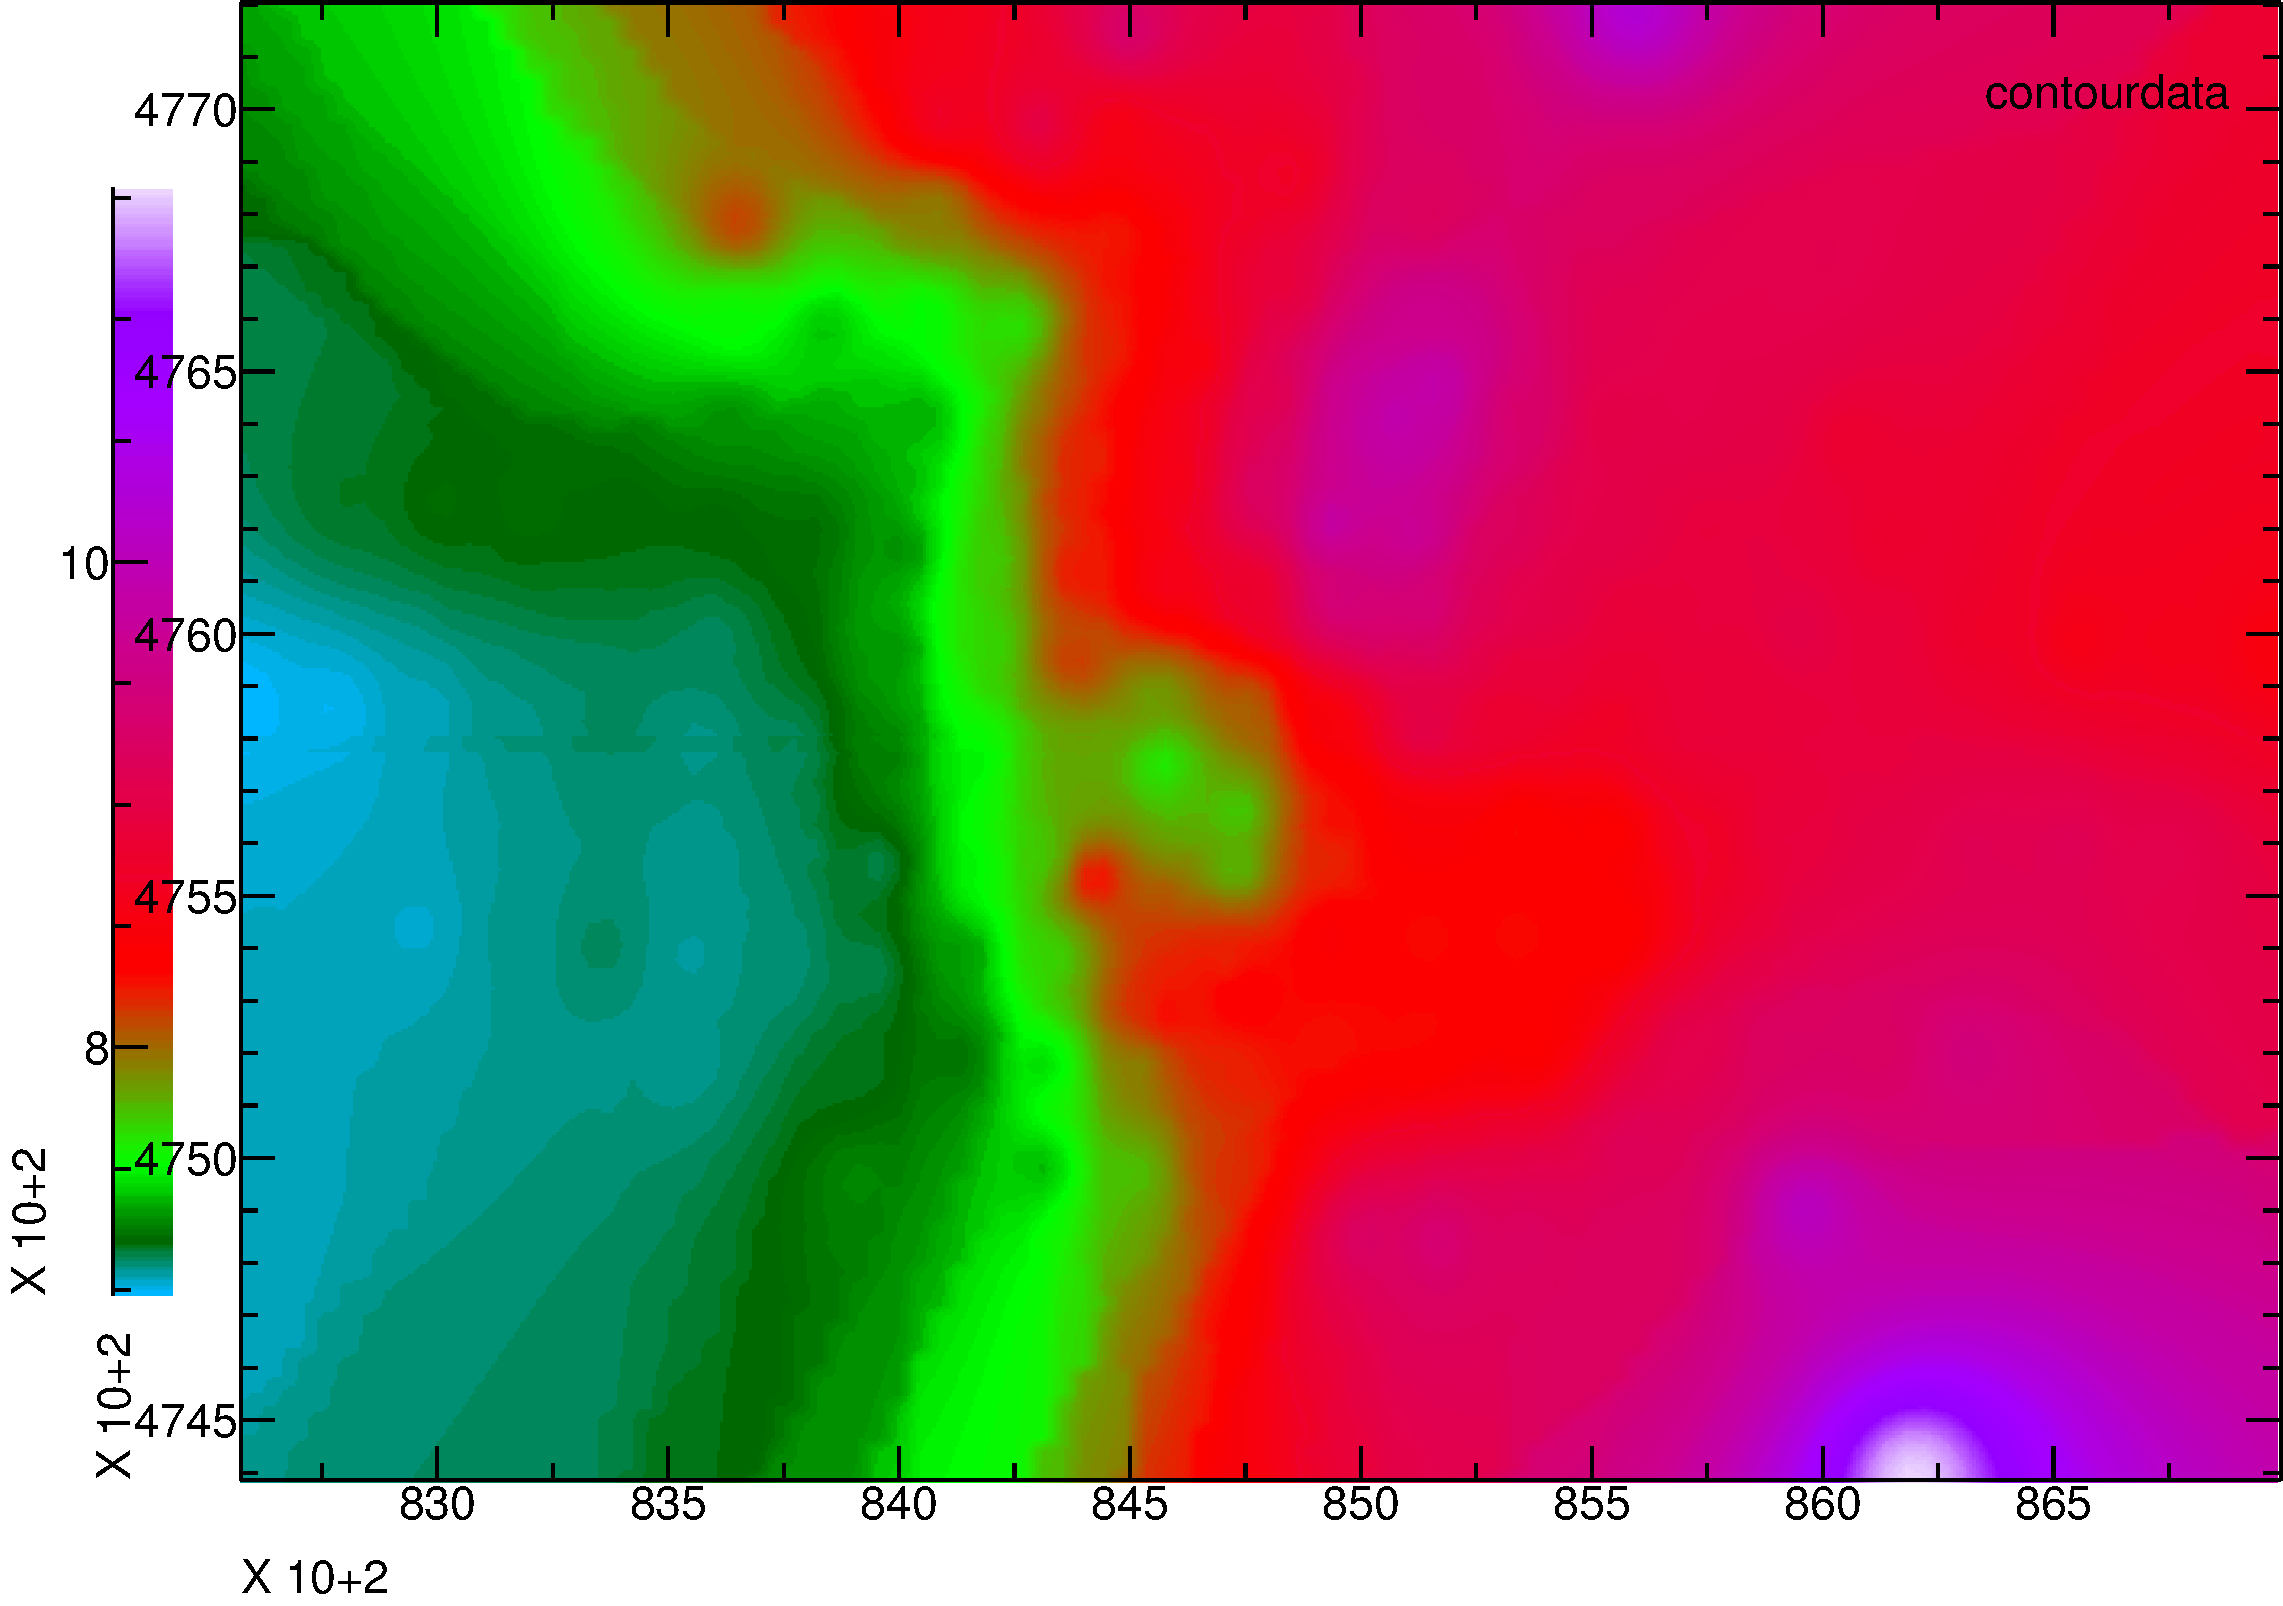
\includegraphics[width=0.9\textwidth]{image}
\caption{image示意图}
\end{figure}

\SACTitle{头段变量}
需要:iftype (设为``IXYZ''), nxsize, nysize

使用:xminimum, xmaximum, yminimum, ymaximum

\SACCMD{inicm}
\label{cmd:inicm}

\SACTitle{概要}
重新初始化SAC

\SACTitle{语法}
\begin{SACSTX}
INICM
\end{SACSTX}

\SACTitle{说明}
此命令可以在任意时刻将SAC初始化到其刚启动的状态。所有活动的图像设备
被终止,全局变量初始化到其初始值,内存中数据丢失。

\SACCMD{installmacro}
\label{cmd:installmacro}

\SACTitle{概要}
将宏文件安装到SAC全局宏目录中

\SACTitle{语法}
\begin{SACSTX}
INSTALLMACRO name [name ...]
\end{SACSTX}

\SACTitle{输入}
\begin{description}
\item [name] SAC宏文件名
\end{description}

\SACTitle{说明}
该命令允许用户将自己写的宏文件安装到SAC全局宏目录(\verb|${SACAUX}/macros|)
中,使得所有人都可以使用。

\SACCMD{int}
\label{cmd:int}

\SACTitle{概要}
利用梯形法或矩形法对数据进行积分

\SACTitle{语法}
\begin{SACSTX}
INT [T!RAPEZEIDAL!|R!ECTANGULAR!]
\end{SACSTX}

\SACTitle{缺省值}
\begin{SACDFT}
int trapezoidal
\end{SACDFT}

\SACTitle{说明}
该命令使用梯形法或矩形法对数据进行数值积分,可以处理等间隔数据或非等间隔数据。除积分之外,
还会根据具体情况修改因变量类型 \texttt{idep},并重新计算 \texttt{depmax}、
\texttt{depmin}、\texttt{depmen}。

对于函数$f(x)$其积分用梯形法表示为
\[
    y_n = y_{n-1} + \frac{1}{2}(x_{n+1}-x_n) (f(x_n)+f(x_{n+1})), \quad n\in[1,npts-1]
\]
用矩形法表示为:
\[
    y_n = y_{n-1} + (x_n-x_{n-1})f(x_n), \quad n\in[1,npts]
\]
二者均有边界条件$y_0=0$。

对于等间隔数据,若使用梯形积分,数据点数 \texttt{npts} 将减1,文件的头段变量
\texttt{b} 将增加半个采样周期\footnote{若使用矩形积分,理论上 \texttt{npts} 和
\texttt{b} 也应有所修改,但实际代码中却未对此多做处理,暂不确定是否是Bug。}。

\SACTitle{头段变量}
depmin、depmax、depmen、idep、npts、b、e

\SACCMD{interpolate}
\label{cmd:interpolate}

\SACTitle{概要}
对等间隔或不等间隔数据进行插值以得到新采样率

\SACTitle{语法}
\begin{SACSTX}
INTERP!OLATE! [D!ELTA! v|N!PTS! v] [B!EGIN! v]
\end{SACSTX}

\SACTitle{输入}
\begin{description}
\item [DELTA v] 设置新采样率为v。数据的时间跨度(E-B)保持不变,npts变化,E由于
    需要与b的间距为delta的整数倍,所以可能会有微调。
\item [NPTS n] 强制设置插值后文件的数据点数为n。时间宽度不变,delta发生变化。
\item [BEGIN v] 在v处开始插值,该值将作为插值文件的起始时间。BEGIN可以和DELTA或NPTS选项
    一起使用。
\end{description}

\SACTitle{说明}
该命令使用Wiggins的weighted average-sloped插值方法将不等间隔数据转换为等间隔数据,
以及对等间隔数据插值得到新的采样率。不像三次样条插值,在输入样本数据点间不会存在
极值。如果要降低采样率,即减采样,由于该命令没有抗混叠滤波器,
所以最好使用 \nameref{cmd:decimate} 命令。

DELTA选项和NPTS选项只能同时使用一个,若二者同时使用,则命令中的后者起作用。

BEGIN选项用于控制输入数据的插值起点,也可以通过cut命令设置b和e再进行插值操作。

\SACTitle{示例}
假定filea是等间隔数据,采样率为0.025,为了将转换到采样率为0.02秒:
\begin{SACCode}
SAC> r filea
SAC> interp delta 0.02
\end{SACCode}
由于新delta小于原数据delta,可能会出现混叠现象,所以会输出警告信息。

假定fileb数据点数npts=3101,想要保持其时间跨度,并采样至npts=4096个点:
\begin{SACCode}
SAC> r fileb
SAC> interp npts 4096
\end{SACCode}

假设filec是不等间隔数据,为了将其转换为采样率为0.01秒的等间隔数据:
\begin{SACCode}
SAC> read filec
SAC> interpolate delta 0.01
\end{SACCode}

\SACTitle{头段变量}
delta、npts、e、b、leven

\SACCMD{keepam}
\label{cmd:keepam}

\SACTitle{概要}
保留内存中谱文件的振幅部分

\SACTitle{语法}
\begin{SACSTX}
!KEEP!AM
\end{SACSTX}

\SACTitle{说明}
该命令会保留谱文件的振幅部分,丢弃相位部分,这样做可以将谱文件的振幅
部分转换为等间隔的数据,可以用SAC的其他命令直接操作。

谱文件可以是振幅-相位格式或实部-虚部格式。若文件以实部-虚部格式存在,
则首先将其转换为振幅-相位格式再丢弃相位部分。

对于实序列,其振幅谱是对称的,因而最终生成的振幅文件仅含npts/2+1个
数据点,数据的文件类型定义为 \texttt{IXY} ,可以跟一般的时间序列区分开。

\SACCMD{khronhite}
\label{cmd:khronhite}

\SACTitle{概要}
对数据应用Khronhite滤波器

\SACTitle{语法}
\begin{SACSTX}
KHRONHITE [v]
\end{SACSTX}

\SACTitle{输入}
\begin{description}
\item [v] 截断频率,单位 \si{\Hz}
\end{description}

\SACTitle{缺省值}
\begin{SACDFT}
khronhite 2.0
\end{SACDFT}

\SACTitle{说明}
此低通滤波器是两个级联的四阶Butterworth低通模拟滤波器的数字近似。
其拐角频率为 \SI{0.1}{\Hz} 以增强Regional地震的基模瑞利波(Rg)的振幅信号。

\SACTitle{头段变量}
depmin、depmax、depmen

\SACCMD{line}
\label{cmd:line}

\SACTitle{概要}
控制绘图中的线型

\SACTitle{语法}
\begin{SACSTX}
LINE [ON|OFF|S!OLID!|D!OTTED!|n] [FILL ON|OFF|pos\_color/neg\_color]
    [I!NCREMENT! [ON|OFF]] [L!IST! STANDARD|nlist]
\end{SACSTX}

\SACTitle{输入}
\begin{description}
\item [ON] 打开线型选项,不改变线型
\item [OFF] 关闭线型选项
\item [SOLID] 改变线型为实线型,并打开线型开关
\item [DOTTED] 改变线型为虚线型,并打开线型开关
\item [n] 设置线型为n并绘制线条。若n取值为0则表示不绘制该线条
\item [FILL ON|OFF] 打开/关闭颜色填充
\item [FILL pos\_color/neg\_color] 对每个数据的正值和负值部分涂色
\item [INCREMENT ON] 每个数据被绘出之后,按照线型表中的次序改变为另一个线型
\item [INCREMENT OFF] 不改变线型
\item [LIST nlist] 改变线型列表
\item [LIST STANDARD] 设置为标准线型列表
\end{description}

\SACTitle{缺省值}
\begin{SACDFT}
line solid increment off list standard
\end{SACDFT}

\SACTitle{说明}
这个命令控制绘图时的线型,图形的框架(轴、标题等等)通常使用实线。
网格的线型用GRID命令控制。并非所有的图形设备都有除实线型之外的其他线型的,
在那些设备上显然这个命令没有什么效果。而对于不同的设备线型号n也可能是不同的。

还有其他命令可以控制数据显示的其他方面。\nameref{cmd:symbol} 命令用于将每个数据点
的值用一个符号显示在图上。
\nameref{cmd:color} 命令控制彩色图形设备的颜色选择。所有的这些属性都是独立的。如果你
想的话你可以选择在每个数据点上选择带符号的蓝色虚线。线型为0代表关闭画线选项。
在LIST选项和 \nameref{cmd:symbol} 命令中可以利用线型为0的特性,在同一张图上将某些
数据用线显示某些数据用符号显示

\SACTitle{示例}
选择依次变化的线型,从线型1开始:
\begin{SACCode}
SAC> line 1 increment
\end{SACCode}

改变线型表使之包含线型3、5和1:
\begin{SACCode}
SAC> line list 3 5 1
\end{SACCode}

使用 \nameref{cmd:plot2} 在同一个图形上绘制三个文件,第一个使用实线无符号,
第二个没有线条,用三角符号,第三个无线条,用十字符号:
\begin{SACCode}
SAC> read file1 file2 file3
SAC> line list 1 0 0 increment
SAC> symbol list 0 3 7 increment
SAC> plot2
\end{SACCode}

将地震图的正值部分涂上红色,负值部分涂上蓝色,如果线型为0,则涂色区域用黑色描边:
\begin{SACCode}
SAC> fg seis
SAC> line 0 fill red/blue
SAC> p
\end{SACCode}

\SACCMD{linefit}
\label{cmd:linefit}

\SACTitle{概要}
对内存中数据的进行最小二乘线性拟合

\SACTitle{语法}
\begin{SACSTX}
LINEFIT
\end{SACSTX}

\SACTitle{说明}
此命令的底层实现与 \nameref{cmd:rmean} 命令是相同的。

对数据使用最小二乘拟合得到一条直线。直线的斜率、y轴截距、斜率的标准差、截距的标准差、
数据的标准差以及数据和模型间的相关系数将分别被写入黑板变量 \texttt{SLOPE}、\texttt{YINT}、
\texttt{SDSLOPE}、\texttt{SDYINT}、\texttt{SDDATA} 和 \texttt{CORRCOEF} 中。

\SACCMD{linlin}
\label{cmd:linlin}

\SACTitle{概要}
设置X、Y轴均为线性坐标

\SACTitle{语法}
\begin{SACSTX}
LINLIN
\end{SACSTX}

\SACCMD{linlog}
\label{cmd:linlog}

\SACTitle{概要}
设置X轴为线性坐标,Y轴为对数坐标

\SACTitle{语法}
\begin{SACSTX}
LINLOG
\end{SACSTX}

\SACCMD{listhdr}
\label{cmd:listhdr}

\SACTitle{概要}
列出指定的头段变量的值

\SACTitle{语法}
\begin{SACSTX}
L!IST!H!DR! [D!EFAULT!|P!ICKS!|SP!ECIAL!] [FILES ALL|NONE|list]
    [COLUMNS 1|2] [INCLUSIVE ON|OFF] [hdrlist]
\end{SACSTX}

\SACTitle{输入}
\begin{description}
\item [DEFAULT] 使用默认的头段变量列表,即列出所有已定义的头段变量
\item [PICKS] 使用picks头段列表,即列出与到时拾取相关的头段变量
\item [SPECIAL] 使用用户自定义的特殊头段变量列表
\item [FILES ALL] 列出内存中所有文件的头段
\item [FILES NONE] 不列出头段,为将来的命令设置默认值
\item [FILES list] 列出部分文件的头段,\texttt{list}是要列出的文件的文件号
\item [COLUMNS 1|2] 输出格式为每行一/两列
\item [INCLUSIVE ON|OFF] \texttt{ON} 表示列出未定义的头段变量的值,
    \texttt{OFF} 则不列出
\item [hdrlist] 指定头段变量列表
\end{description}

\SACTitle{缺省值}
\begin{SACDFT}
listhdr default files all columns 1 inclusive off
\end{SACDFT}

\SACTitle{说明}
该命令可以列出指定的头段变量的值,用户可以使用默认列表 \texttt{DEFAULT}
列出全部头段变量,或 \texttt{PICKS} 列出与到时拾取相关的头段变量,
包括 \texttt{B}、\texttt{E}、\texttt{O}、\texttt{A}、\texttt{Tn}、
\texttt{KZTIME}、\texttt{KZDATE}。用户可以自定义一个特殊列表并通过
\texttt{SPECIAL} 选项再次使用该列表。

该命令的输出包含头段变量名、一个等于号以及头段变量的当前值。未定义的
头段变量的值用 \texttt{undefined} 表示。

\SACTitle{示例}
获取 \texttt{picks} 列表,输出为两列显示:
\begin{SACCode}
SAC> lh picks column 2
\end{SACCode}

获得第三、四个文件的默认头段列表:
\begin{SACCode}
SAC> lh files 3 4
\end{SACCode}

列出文件开始和结束时间:
\begin{SACCode}
SAC> lh b e
\end{SACCode}

定义一个包含台站参数的特殊列表:
\begin{SACCode}
SAC> lh kstnm stla stlo stel stdp
\end{SACCode}

稍后再次使用上面的特殊列表:
\begin{SACCode}
SAC> lh special
\end{SACCode}

为后面的 \texttt{lh} 命令设置输出为两列:
\begin{SACCode}
SAC> lh columns 2 files none
\end{SACCode}

\SACCMD{load}
\label{cmd:load}

\SACTitle{概要}
导入外部命令(在SAC的linux版本中外部命令的导入需要额外的工作)

\SACTitle{语法}
\begin{SACSTX}
LOAD comname [ABBREV abbrevname]
\end{SACSTX}

\SACTitle{输入}
\begin{description}
\item [comname] 从一个共享目标文件中载入的一个外部函数名
\item [ABBREV abbrevname] 命令的简写
\end{description}

\SACTitle{说明}
这个命令允许用户载入由SAC外部命令接口写的命令。(参见EXTERNAL\_INTERFACE文档)。这个命令必须是一个储存在共享目标库(.so文件)中。SAC将检查所有环境变量SACSOLIST中的共享目标库,这个环境变量需要包含一个或多个共享目标库,每个库以空格分割。到这些共享目标库的路径必须在环境变量LD\_LIBRARY\_PATH中指定。如果SACSOLIST为设置,则SAC将使用由LD\_LIBRARY\_PATH中指定的路径在共享文件库libsac.so中寻找。一个叫做libcom.so的库随着SAC发布。

\SACTitle{示例}
设置你的环境变量使得SAC在当前目录从库文件libbar.so中查找一个称为foo的命令,并为foo设置别名为myfft:
\begin{SACCode}
% export SACSOLIST = "libcom.so libbar.so"
#  Add the current directory to the search path.
% export LD_LIBRARY_PATH {$LD_LIBRARY_PATH}:.
% sac
SAC> load foo abbrev myfft* load the command
SAC> read file1.z file2.z file3.z
SAC> myfft real-imag* invoke command with its arguments,
* commands must parse their own args.
SAC> psp
\end{SACCode}

如何创建一个包含你的命令的共享目标库:
\begin{SACCode}
Solaris::
cc -o libxxx.so -G extern.c foo.c bar.c
SGI::
cc -g -o libxxx.so -shared foo.c bar.c
LINUX: (gcc)::
gcc -o libxxx.so -shared extern.c foo.c bar.c sac.a
\end{SACCode}
其中sac.a可以从你得到sac的地方获得

\SACTitle{SAC发布的外部命令}
在SAC的发布版中有一个外部命令,叫做FLIPXY。FLIPXY将一个或多个X-Y数据文件
作为输入,并调换X和Y。这个命令在 \verb|${SACAUX}/external| 中的libcom.so
中,同时还有FLIPXY的源代码作为参考。为了导入FLIPXY,libcom.so必须包含在
\verb|$SACSOLIST| 中。

\SACCMD{loadctable}
\label{cmd:loadctable}

\SACTitle{概要}
允许用户在彩色绘图中选择一个新的颜色表

\SACTitle{语法}
\begin{SACSTX}
L!OAD!CT!ABLE! n|[DIR CURRENT|name] [filelist]
\end{SACSTX}

\SACTitle{输入}
\begin{description}
\item [n] 标准SAC颜色表对于的号,n可以取1-17
\item [DIR CURRENT] 从当前目录载入颜色表,当前目录指的是你启动SAC的目录
\item [DIR name] 从目录name中载入颜色表,这是一个相对或绝对目录名
\item [filelist] 颜色表文件列表
\end{description}

\SACTitle{说明}
这个命令允许用户选择一个新的颜色表或者通过指定颜色表的文件以及路径提供他们自己的颜色表。
如果未使用DIR选项,SAC将首先在 \verb|$SACAUX| 中寻找颜色表,然后在用户的工作目录中寻找.

*在SACAUX下可以的ctables下有21个文件,其中一个为gmt.cpt,用于在SAC中绘制与GMT有关的彩色图形,另外20个文件为三列数据,应该就是颜色表了,前面说的n取1到17可能有些过时了。具体谁对应谁还不清楚,just try them!

\SACCMD{log}
\label{cmd:log}

\SACTitle{概要}
对每个数据点取其自然对数($\ln y$)

\SACTitle{语法}
\begin{SACSTX}
LOG
\end{SACSTX}

\SACTitle{头段变量}
depmin、depmax、depmen

\SACCMD{log10}
\label{cmd:log10}

\SACTitle{概要}
对每个数据点取以10为底对数($\log_{10} y$)

\SACTitle{语法}
\begin{SACSTX}
LOG10
\end{SACSTX}

\SACTitle{头段变量}
depmin、depmax、depmen

\input{commands/loglab}
\SACCMD{loglin}
\label{cmd:loglin}

\SACTitle{概要}
设置X轴为对数坐标,Y轴为线性坐标

\SACTitle{语法}
\begin{SACSTX}
LOGLIN
\end{SACSTX}

\SACCMD{loglog}
\label{cmd:loglog}

\SACTitle{概要}
设置X、Y轴均为对数坐标

\SACTitle{语法}
\begin{SACSTX}
LOGLOG
\end{SACSTX}

\SACCMD{lowpass}
\label{cmd:lowpass}

\SACTitle{概要}
对数据文件应用一个无限脉冲低通滤波器

\SACTitle{语法}
\begin{SACSTX}
L!OW!P!ASS! [BU!TTER!|BE!SSEL!|C1|C2] [C!ORNERS! v1 v2] [N!POLES! n] [P!ASSES! n]
    [T!RANBW! v] [A!TTEN! v]
\end{SACSTX}

\SACTitle{输入}
\begin{description}
\item [BUTTER] 应用一个Butterworth滤波器
\item [BESSEL] 应用一个Bessel滤波器
\item [C1] 应用一个Chebyshev I型滤波器
\item [C2] 应用一个Chebyshev II滤波器
\item [CORNERS v1 v2] 设定拐角频率分别为v1和v2,即频率通带为v1--v2
\item [NPOLES n] 设置极数为N,范围:1--10
\item [PASSES n] 设通道数为N,范围:1--2
\item [TRANBW v] 设置Chebyshev转换带宽为v
\item [ATTEN v] 设置Chebyshev衰减因子为v
\end{description}

\SACTitle{缺省值}
\begin{SACDFT}
lowpass butter corner 0.2 npoles 2 passes 1 tranbw 0.3 atten 30
\end{SACDFT}

\SACTitle{说明}
参见 \nameref{cmd:bandpass} 命令的相关说明。

\SACTitle{示例}
应用一个四极Butterworth,拐角频率为 \SI{2}{\Hz}:
\begin{SACCode}
SAC> lp n 4 c 2
\end{SACCode}

在此之后如果要应用一个二极双通具有相同频率的Bessel:
\begin{SACCode}
SAC> lp n 2 be p 2
\end{SACCode}

\SACTitle{头段变量改变}
depmin、depmax、depmen

\SACCMD{macro}
\label{cmd:macro}

\SACTitle{概要}
执行SAC宏文件

\SACTitle{语法}
\begin{SACSTX}
M!ACRO! name [arguments]
\end{SACSTX}

\SACTitle{输入}
\begin{description}
\item [name] 要执行的SAC宏文件名
\item [arguments] 宏文件参数
\end{description}

\SACTitle{说明}
参考 \nameref{sec:macros} 一节。

\SACCMD{map}
\label{cmd:map}

\SACTitle{概要}
利用SAC内存中的所有数据文件生成一个包含台站/事件符号、地形以及台站名的
GMT地图,也可以在命令行上指定一个事件文件。每个
地震事件符号可以根据震级、残差等确定其大小。这个命令会产生一个ps文件,
并将该文件在屏幕上显示,同时产生一个绘制该图的shell脚本。

\SACTitle{语法}
\begin{SACSTX}
MAP [MER!CATOR!|EQ!UIDISTANT!|AZ!IMUTHAL_EQUIDISTANT!|ROB!INSON!]
    [WEST minlon] [EAST maxlon] [NORTH maxlat] [SOUTH minlat]
    [MAG!NITUDE!|RE!SIDUAL!|RM!EAN_RESIDUAL!] [EV!EVNTFILE! filename]
    [TOPO!GRAPHY!] [STAN!AMES!] [MAPSCALE on|off] [PLOTSTATIONS on|off]
    [PLOTEVENTS on|off] [PLOTLEGEND on|off] [LEGENDXY x y]
    [FILE output-file]
\end{SACSTX}

\SACTitle{输入}
SAC中可以使用的投影方式包括:
\begin{itemize}
\item MERCATOR:	投影方式为Mercator投影。
\item EQUIDISTANT: 投影方式为等间距圆柱投影,经纬度为线性。
\item ROBINSON: 投影方式为Robinson投影,适用于世界地图。
\item LAMBERT: 适用于东西范围较大的区域。
\item UTM:通用横向Mercator(尚未实现)。
\end{itemize}

下面的选项允许用户指定地图的区域,其默认使用台站以及事件经纬度的最小最大值(如果
真是如此,这样的缺省值并不合适,因为那样意味着某些台站或事件将位于地图的边界处,
但是实际上地图范围给的还是不错的):
\begin{itemize}
\item WEST :  地图的最小经度
\item EAST : 地图的最大经度
\item NORTH : 地图的最大纬度
\item SOUTH : 地图的最小纬度
\item AUTOLIMITS:  自动决定地图的区域 [缺省值]
\end{itemize}

下面的选项允许用户向地图中添加位置和注释:
\begin{itemize}
\item STANames on | off :  在地图上绘制台站名[默认为off]
\item MAPSCALE on | off :  在地图上绘制地图比例尺[默认为off]
\item PLOTSTATIONS on | off : 绘制地震图给出的全部台站[默认为on]
\item PLOTEVENTS on | off : 绘制eventfile和/或地震图给出的全部事件[默认为on]
\end{itemize}

下面的选项允许用户根据不同的值给出不同地震事件符号的大小。默认值是所有符号大小一样:
\begin{itemize}
\item MAGnitude : user0定义地震震级,user0越大,则事件符号越大。
\item REsidual : user0定义残差。根据user0的绝对值定义事件符号的大小。正值为(+) 负值为(-).
\item RMean\_residual : 与residual相同,除了将所有残差去除均值之外
\item PLTLEGEND on | off : 绘制地震震级以及残差的图例[默认为on]
\item LEGENDXY x y : 绘制图例的绝对位置,默认为[1,1]。位置是相对于页面的左下角,
    其单位为inch。这是一个与地震震级和残差有关的图例。
\item EVENTFILE : 指定一个自由格式的ASCII文本文件,其包含了额外的事件数据,文件的
    每一行包含单个事件的数据。每行的头两列必须包含纬度和经度(单位为度)。第三列可以
    包含符号大小信息(比如震级、深度、走时残差等)。
\item TOPOgraphy on | off : 设置TOPO为开允许用户向地图中添加地形和海洋深度。这个命令
    读取GMT中grdraster.info的第一个地形文件,当然地形文件中必须要有该区域的数据。
    地形彩色图使用 \verb|$SACAUX/ctables/gmt.cpt|。网格文件被写入当前目录
\item FILE : 默认的输出文件名为gmt.ps,你可以通过FILE选项指定文件名
\end{itemize}
可以用SAC的 \nameref{cmd:title} 命令指定地图标题。

\SACTitle{缺省值}
\begin{SACDFT}
map mercator topo off stan off file gmt.ps plotstations on
    plotevents on
\end{SACDFT}

\SACTitle{示例}
利用SAC提供的一些数据作为例子:
\begin{SACCode}
SAC> dg sub regional *.z
SAC> title "Station Location Map"
SAC> map stan on
Using Default Postscript Viewer
	gs -sDEVICE=x11 -q -dNOPROMPT -dTTYPAUSE
\end{SACCode}
绘制出的地图如图 \ref{fig:map} 所示,整个地图的边界控制的还算不错,还算比较美观,
三角形代表台站位置,圆形代表地震位置,大小也控制的不错。生成这个图的同时,还有
一个可以用于生成该地图的shell脚本。

默认情况下,该命令会自动使用gs预览生成的PS文件。如果想用其他PS阅读器预览,可以
通过修改环境变量 \texttt{SACPSVIEWER} 来实现,比如 \texttt{export SACPSVIERER=evince}。

\begin{figure}[!ht]
\centering
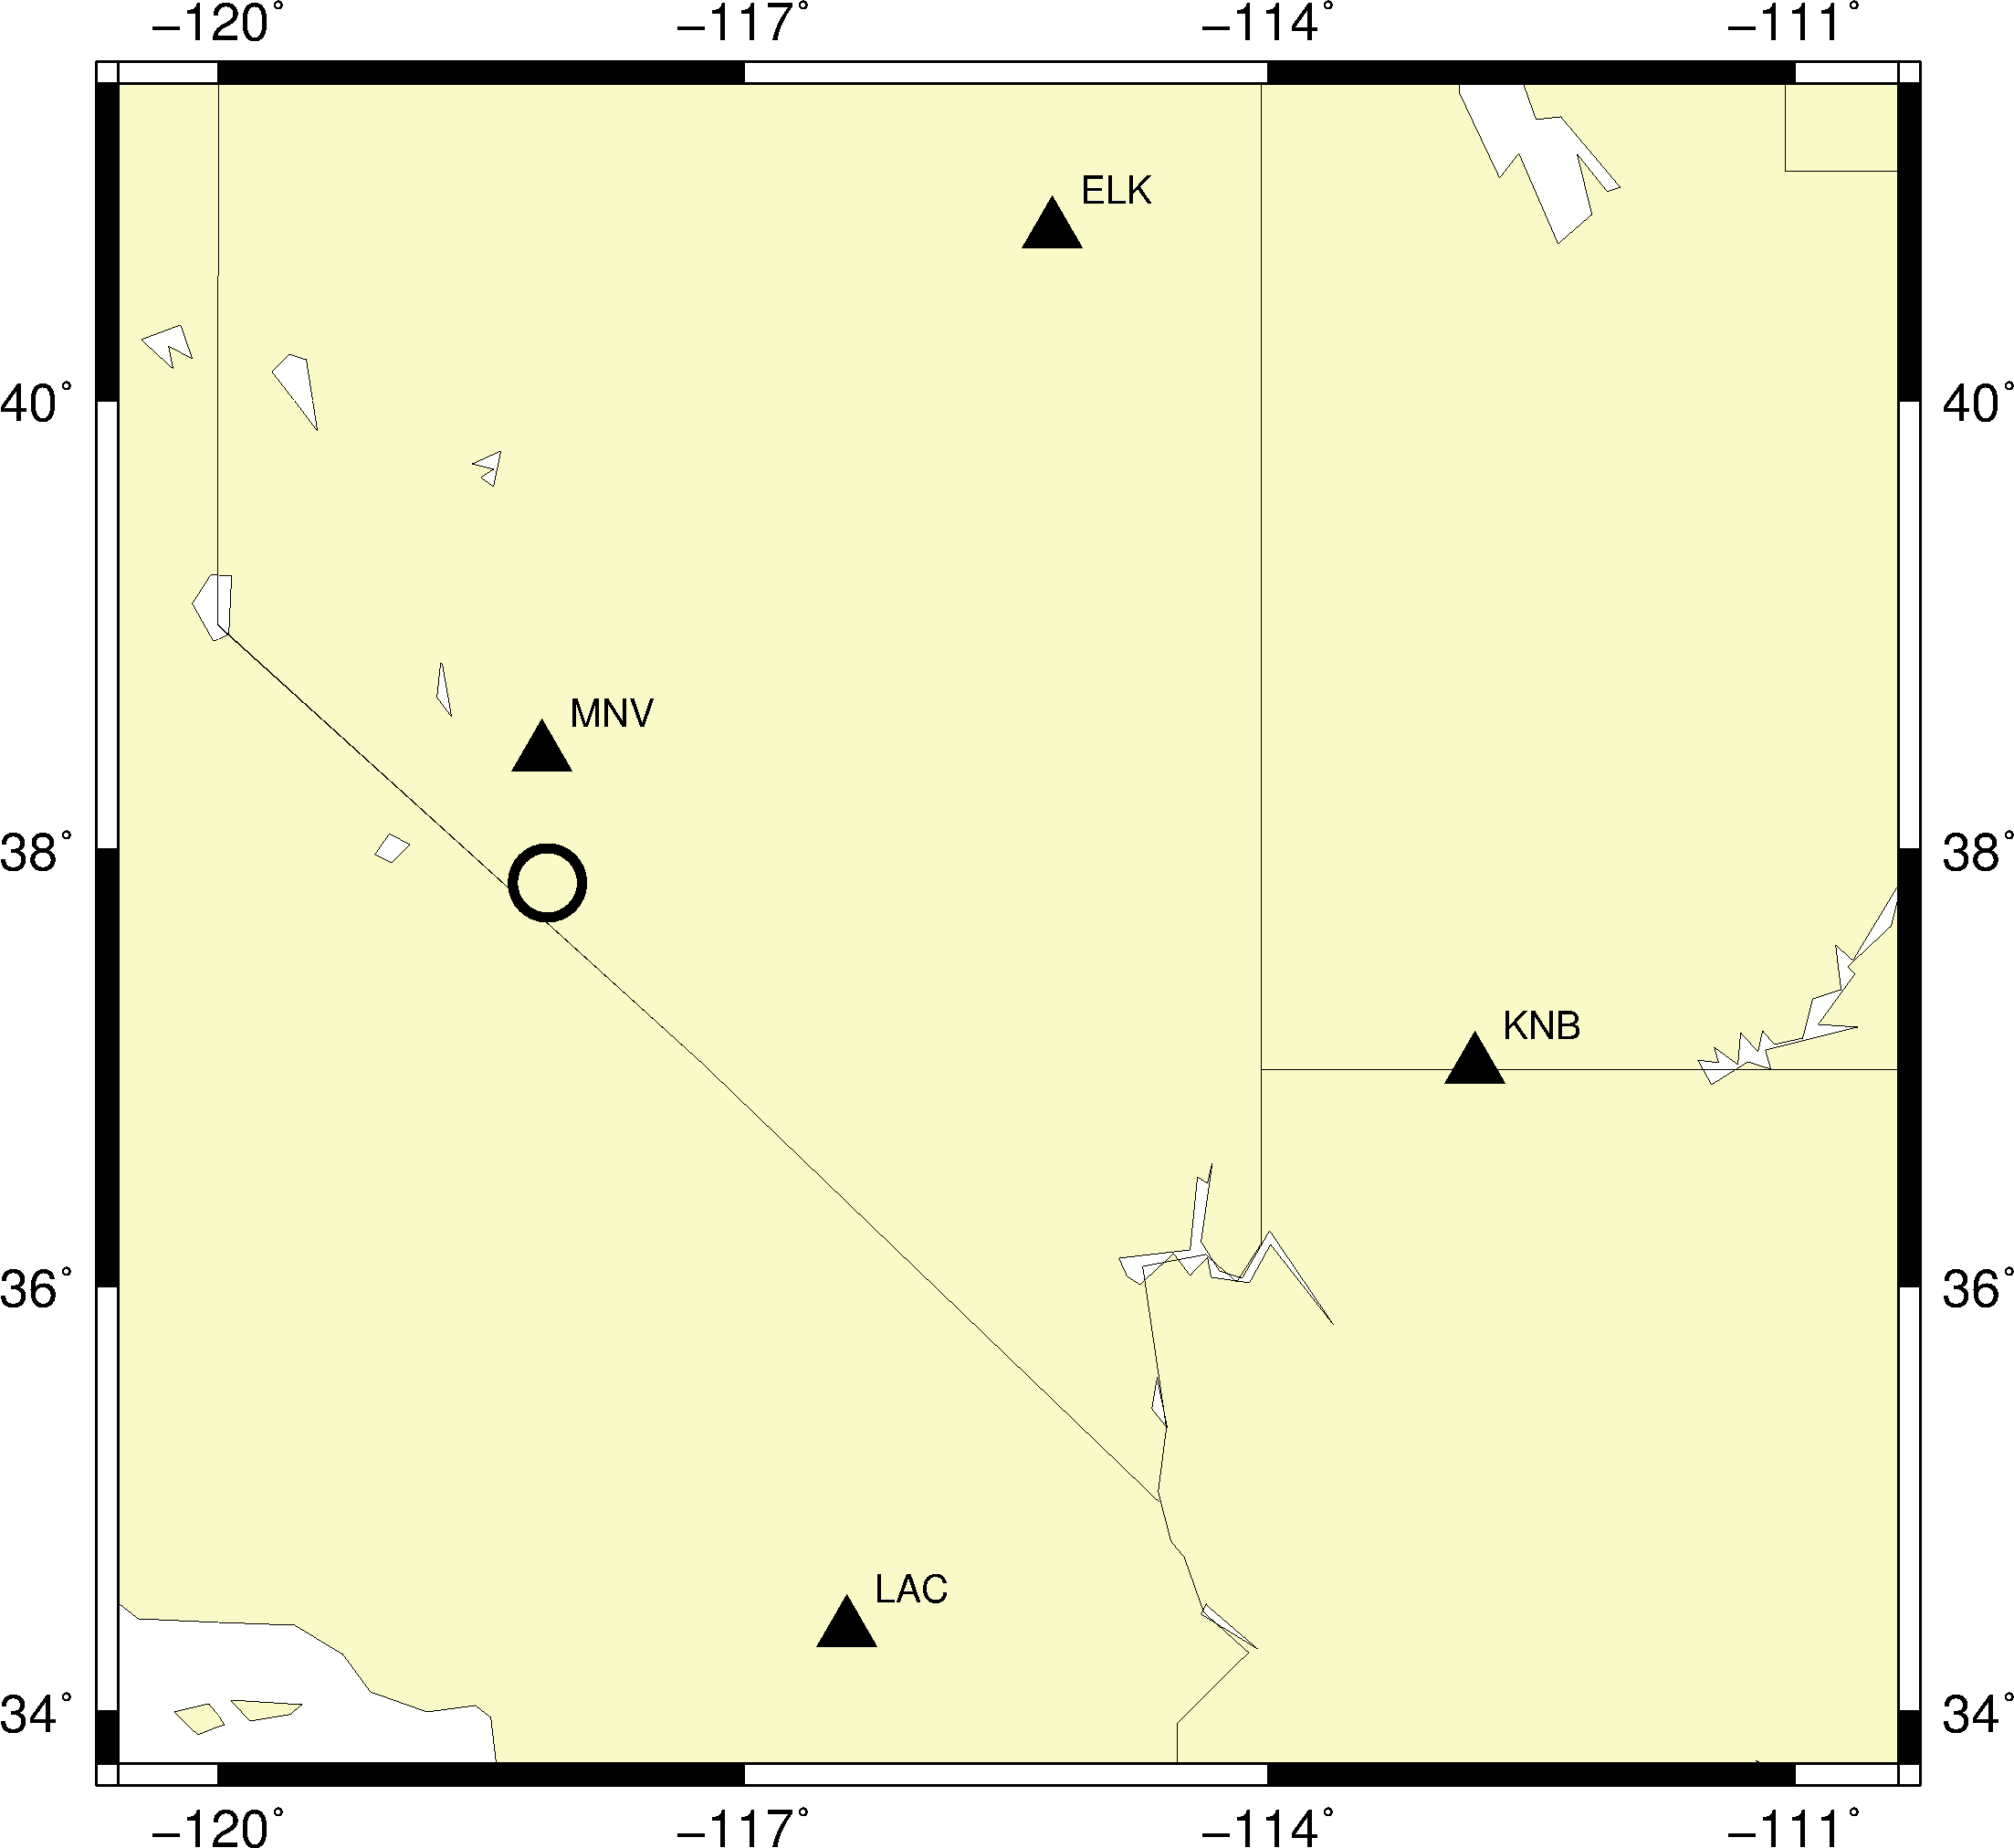
\includegraphics[width=0.7\textwidth]{map}
\caption{map绘制地震、台站分布图}
\label{fig:map}
\end{figure}

\SACTitle{头段数据}
台站纬度(stla)以及经度(stlo)必须在头段中被定义。如果事件纬度(evla)以及经度(evlo)
被定义则其会被包含在地图中。如果这个命令在执行BBFK之后执行,MAP将沿着反方位角方向
绘制大圆弧路径。这个版本的MAP是基于4.0版本的Generic Mapping Tools,要执行这个命令,
你需要将GMT4.0安装在你的机器上并保证可执行文件位于路径中。

每个MAP命令的结果将写入当前目录下一个称为gmt.csh的脚本中。用户可以修改这个文件
以利用更多SAC未利用的选项。默认单位是inch,当然可以在脚本中修改。

在使用pscoast绘制海岸线时,SAC采用了 \texttt{-Dl} 选项,其中l代表低精度的海岸线数据。用户
可以在脚本中修改使用更高精度的海岸线数据。
\SACCMD{markptp}
\label{cmd:markptp}

\SACTitle{概要}
测量并标记信号在测量时间窗内的最大峰峰值

\SACTitle{语法}
\begin{SACSTX}
MARKP!TP! [L!ENGTH! v] [T!O! marker]
\end{SACSTX}

\SACTitle{输入}
\begin{description}
\item [LENGTH v] 设置滑动窗的长度为v秒
\item [TO marker] 指定某个时间标记头段用于保存最小值的所对应的时刻;最大值所对应
    的时刻保存在下一个时间标记头段中。时间标记头段marker可以取Tn(n=0--9)。
\end{description}

\SACTitle{缺省值}
\begin{SACDFT}
markptp length 5.0 to t0
\end{SACDFT}

\SACTitle{说明}
该命令会计算信号在测量时间窗内的最大峰峰值。所谓最大峰峰值,即最大振幅与最小
振幅的振幅差。测量结果中,最小值(波谷)所对应的时刻会写到 \texttt{TO marker} 中所
指定的时间标记头段中,最大值(波峰)所对应的时刻会写到相应的下一个时间标记头段中。
最大峰峰值保存到 \texttt{user0} 中,\texttt{kuser0} 中的值为 \texttt{PTPAMP}。
如果使用 \nameref{cmd:oapf} 打开了字符数字型震相拾取文件,则该命令的结果也会写入到
文件中。

默认情况下,测量时间窗为整个信号,可以使用 \nameref{cmd:mtw} 命令设置新的测量时间窗。
同时,在测量时还需要设置滑动时间窗(sliding time window)的长度。滑动窗的工作原理是,
首先将长度为 \texttt{v} 的滑动窗置于测量时间窗的起始位置,搜索该滑动窗内的最大峰峰值,
然后将长度为 \texttt{v} 的滑动窗向右移动一个数据点,并搜索该滑动窗内的最大峰峰值,
以此类推,直到滑动窗的右边界与测量时间窗的右边界重合为止,此时将有多个最大峰峰值,
最后返回所有最大峰峰值中最大的一个。

对于滑动时间窗(sliding time window)的长度,若stw的长度大于mtw的长度,则 \texttt{stw=mtw};
若stw的长度小于等于零,则 \texttt{stw=mtw/2}。

\SACTitle{示例}
设置测量时间窗为头段T4和T5之间,并使用默认的滑动时间窗长和时间标记:
\begin{SACCode}
SAC> mtw t4 t5
SAC> markptp
SAC> lh t0 t1 user0 kuser0
\end{SACCode}

设置测量时间窗为初动之后的 \SI{30}{s},滑动时间窗为 \SI{3}{s},起始时间标记为T7:
\begin{SACCode}
SAC> mtw a 0 30
SAC> markptp l 3. to t7
SAC> lh t7 t8 user0 user1
\end{SACCode}

\SACTitle{头段变量}
Tn、KTn、user0、kuser0

\SACTitle{源码}
\texttt{src/smm/xmarkptp.c}、\texttt{src/smm/ptp.c}

\SACCMD{marktimes}
\label{cmd:marktimes}

\SACTitle{概要}
根据一个速度集得到走时并对数据文件进行标记

\SACTitle{语法}
\begin{SACSTX}
MARKT!IMES! [T!O! marker] [D!ISTANCE! H!EADER!|v] [O!RIGIN! H!EADER!|v|GMT time]
    [V!ELOCITIES! v ... ]
\end{SACSTX}

\SACTitle{输入}
\begin{description}
\item [TO marker] 定义头段中用于储存结果的第一个时间标记。对下一个的速度使用下一个时间
\item [marker]  T0|T1|T2|T3|T4|T5|T6|T7|T8|T9
\item [DISTANCE HEADER] 使用头段中的DIST代表距离用于走时计算
\item [DISTANCE v] 使用v作为走时计算中的距离
\item [ORIGIN HEADER] 使用头段中的参考时间(O)用于走时计算
\item [ORIGIN v] 使用相对参考时间偏移v秒用于走时计算
\item [ORIGIN GMT time] 使用Greenwich平均时间作为参考时间
\item [time] GMT时间包含六个整数:年、儒略日、时、分、秒、毫秒
\item [VELOCITIES v ... ] 设置用于走时计算的速度集,最多可以输入10个速度
\end{description}

\SACTitle{缺省值}
\begin{SACDFT}
marktimes velocities 2. 3. 4. 5. 6. distance
    header origin header to t0
\end{SACDFT}

\SACTitle{说明}
这个命令在头段中标记震相的到时,给定事件的发生时间,震中距以及速度即可计算到	时。下面的方程用于简单估计走时:
 		\[ time(j) = origin + \frac{distance}{velocity(j)} \]
结果被写入指定的时间标记中

\SACTitle{示例}
使用默认的速度集,强制距离为 \SI{340}{\km},第一个时间标记为T4:
\begin{SACCode}
SAC> marktimes distance 340. to t4
\end{SACCode}

选择一个不同的速度集:
\begin{SACCode}
SAC> markt v 3.5 4.0 4.5 5.0 5.5
\end{SACCode}

设置新的参考时间并将结果保存在T2中:
\begin{SACCode}
SAC> markt origin gmt 1984 231 12 43 17 237 to t2
\end{SACCode}

\SACTitle{头段变量改变}
Tn, KTn

\SACCMD{markvalue}
\label{cmd:markvalue}

\SACTitle{概要}
在数据文件中搜索并标记某个值

\SACTitle{语法}
\begin{SACSTX}
MARKV!ALUE! [GE|LE v] [TO marker]
\end{SACSTX}

\SACTitle{输入}
\begin{description}
\item [GE v] 搜索并标记第一个大于或等于v的数据点
\item [LE v] 搜索并标记第一个小于或等于v的数据点
\item [TO marker] 用于保存数据点的时刻的时间标记头段,marker可以取Tn(n=0--9)
\end{description}

\SACTitle{缺省值}
\begin{SACDFT}
markvalue ge 1 to t0
\end{SACDFT}

\SACTitle{说明}
该命令会在信号的测量时间窗内搜索第一个满足条件(大于或等于/小于或等于)的数据点,
并将该数据点所对应的时刻记录下来。默认情况下,测量时间窗为整个信号,可以
使用 \nameref{cmd:mtw} 命令设置新的测量时间窗。

\SACTitle{示例}
搜索文件中第一个值大于3.4的点并将结果保存在头段T7中:
\begin{SACCode}
SAC> markvalue ge 3.4 to t7
\end{SACCode}

设定测量时间窗为T4后的10秒,并搜索第一个小于-3的值:
\begin{SACCode}
SAC> mtw t4 0 10
SAC> markvalue le -3 to t5
\end{SACCode}

\SACTitle{头段变量改变}
Tn、KTn

\input{commands/mathop}
\SACCMD{merge}
\label{cmd:merge}

\SACTitle{概要}
将多个数据文件合并成一个文件

\SACTitle{语法}
\begin{SACSTX}
MERGE [V!ERBOSE!] [G!AP! Z!ERO!|I!NTERP!] [O!VERLAP! C!OMPARE!|A!VERAGE!] [filelist]
\end{SACSTX}

\SACTitle{输入}
\begin{description}
\item [VERBOSE] 合并数据时在终端显示合并的细节
\item [GAP ZERO|INTERP] 如何处理数据间断。\texttt{ZERO} 表示将数据间断
    处补零值;\texttt{INTERP} 表示对数据间断处进行线性插值
\item [OVERLAP COMPARE|AVERAGE] 如何处理数据重叠。\texttt{COMPARE} 表示
    对重叠的时间段内的数据进行比较,若不匹配则退出;\texttt{AVERAGE} 表
    示对重叠时间段内的数据进行平均
\item [filelist] SAC二进制数据文件列表(暂不支持通配符)
\end{description}

\SACTitle{说明}
该命令用于将一系列时间上相邻的数据文件首尾相连合并成一个文件。在合并数据
时,会先检查要合并的文件是否有相同的 \texttt{kstnm}、\texttt{kentwk}、
\texttt{kcmpnm}、\texttt{delta}。

在SAC v101.6中完全重新了该命令,因而该命令的功能和语法与之前的版本有所
不同。

在v101.6之前的版本中,\texttt{merge} 命令的用法与 \nameref{cmd:addf} 命令的
用法相似。该命令会将内存中的文件依次分别与filelist中的文件进行合并,且内存中的文件的
开始时刻必须早于filelist中的文件的开始时刻。因而在将多个数据文件合并成一个文件时,只能
先读取第一段数据,然后 \texttt{merge} 第二段数据,再 \texttt{merge} 第三段数据,
依次不断循环执行。

旧版本的 \texttt{merge} 命令用起来相对复杂。需要多次执行 \texttt{merge} 命令,且
需要用户自己判断波形文件的先后顺序。

v101.6之后的新版 \texttt{merge} 命令,会将内存中的全部数据文件以及filelist中的
全部文件合并成单个文件。若内存中无数据,则只合并filelist中的数据文件;若filelist为空,
则只合并内存中的数据文件。且新版的 \texttt{merge} 命令可以合并任意数目和任意顺序的
数据文件。

若要合并的数据段之间存在间断,可以通过补零或线性插值的方式弥补间断;若数据段之间
存在重叠,可对重叠的部分进行比较,判断重叠的区域内振幅是否匹配,或者直接进行振幅的平均。

\SACTitle{示例}
下面看一个数据合并的示例:
\begin{SACCode}
SAC> read file1 file2
SAC> merge file3 file4
\end{SACCode}
在v101.6之前的版本中,本示例的运行结果是:file3与file1合并成文件file1,file4与
file2合并成文件file2,此时内存中有两个文件file1和file2。而在v101.6及其之后的版本中,
这个例子的结果是,文件file1、file2、file3、file4合并成文件file1,此时内存中只有
一个文件file1。这样的修改使得不同版本的语法不兼容,但实际使用时新版的 \texttt{merge}
命令要更方便也更符合人的正常思维。

下面介绍几个新版本的 \texttt{merge} 命令的用法示例。

多个文件合并成单个文件的一种方法:
\begin{SACCode}
SAC> r file1                        // 读取一个文件
SAC> merge file2 file3 file4        // merge其余文件
SAC> w over
\end{SACCode}

另一种合并办法:
\begin{SACCode}
SAC> r file1 file2 file3 file4
SAC> merge                      // 合并内存中的所有文件
SAC> w over                     // 合并后的文件写入到file1中
\end{SACCode}

再一种合并方法:
\begin{SACCode}                     
                                    // 内存中无数据
SAC> merge file1 file2 file3 file4  // 合并filelist中的全部文件
SAC> w over                         // 保存到file1中
\end{SACCode}

\SACTitle{头段变量改变}
npts、depmin、depmax、depmen、e

\SACCMD{message}
\label{cmd:message}

\SACTitle{概要}
发送信息到用户终端

\SACTitle{语法}
\begin{SACSTX}
MES!SAGE! text
\end{SACSTX}

\SACTitle{输入}
\begin{description}
\item [text] 要发送到终端的信息文本。若文本中有空格则必须用引号括起来
\end{description}

\SACTitle{说明}
此命令用于在SAC宏文件执行时发送状态或其他信息给用户,在交互式模式下一般
没有用(除非你想自己跟自己聊天,如示例所示)。

\SACTitle{示例}
发送无空格的信息:
\begin{SACCode}
SAC> message finished
 finished
\end{SACCode}

发送带有空格的信息,需要加上单引号或双引号:
\begin{SACCode}
SAC> message 'Job has finished.'
 Job has finished.
\end{SACCode}

\SACCMD{mtw}
\label{cmd:mtw}

\SACTitle{概要}
设置某些测量命令中的测量时间窗(measurement time window)

\SACTitle{语法}
\begin{SACSTX}
MTW [ON|OFF|pdw]
\end{SACSTX}

\SACTitle{输入}
\begin{description}
\item [ON] 打开测量时间窗选项但不改变窗的值
\item [OFF] 关闭测量时间窗选项,测量命令将对整个文件进行操作
\item [pdw] 打开测量时间窗并设置其新值。pdw的用法参考 \nameref{subsec:pdw} 一节
\end{description}

\SACTitle{缺省值}
\begin{SACDFT}
mtw off
\end{SACDFT}

\SACTitle{说明}
SAC中与测量有关的命令有 \nameref{cmd:markptp} 和 \nameref{cmd:markvalue} 。
当不设置mtw时,测量命令会对整个文件进行操作;当设置了mtw时,测量命令仅mtw时间
窗内的数据执行测量命令。

\SACTitle{相关命令}
\nameref{cmd:cut}、\nameref{cmd:markptp}、\nameref{cmd:markvalue}

\SACCMD{mul}
\label{cmd:mul}

\SACTitle{概要}
给每个数据点乘以同一个常数

\SACTitle{语法}
\begin{SACSTX}
MUL [v1 [v2 ... vn]]
\end{SACSTX}

\SACTitle{输入}
\begin{description}
\item [v1] 乘到第一个文件的常数
\item [v2] 乘到第二个文件的常数
\item [vn] 乘到第n个文件的常数
\end{description}

\SACTitle{缺省值}
\begin{SACDFT}
mul 1.0
\end{SACDFT}

\SACTitle{说明}
参见 \nameref{cmd:add} 的相关说明。

\SACTitle{头段变量改变}
depmin、depmax、depmen

\SACCMD{mulf}
\label{cmd:mulf}

\SACTitle{概要}
使内存中的一组数据乘以另一组数据

\SACTitle{语法}
\begin{SACSTX}
MULF [NEWHDR [ON|OFF]] filelist
\end{SACSTX}

\SACTitle{输入}
\begin{description}
\item [NEWHDR ON|OFF] 若为OFF,则生成的数据文件使用内存中原文件的头段;
    若为ON,则生成的数据文件使用filelist中新文件的头段。缺省值为OFF。
\item [filelist] SAC二进制文件列表。
\end{description}

\SACTitle{说明}
参见 \nameref{cmd:addf} 命令的相关说明。

\SACTitle{示例}
参见 \nameref{cmd:addf} 命令的相关示例。

\SACTitle{头段变量}
depmin、depmax、depmen、npts、delta

\SACTitle{相关命令}
\nameref{cmd:read}、\nameref{cmd:binoperr}

\SACCMD{mulomega}
\label{cmd:mulomega}

\SACTitle{概要}
在频率域进行微分操作

\SACTitle{语法}
\begin{SACSTX}
MULOMEGA
\end{SACSTX}

\SACTitle{说明}
根据傅里叶变换的微分性质:
\[
\mathcal{F}[f'(x)]= i \omega \mathcal{F}[f(x)]
\]
其中$\omega = 2 \pi f $,即函数微分在频率域可以用简单的乘法来表示。

该命令仅可对谱文件进行操作,谱文件可以是振幅-相位型或实部-虚部型。

若为振幅-相位型:
\[
\mathcal{F}[f'(x)]= i \omega \mathcal{F}[f(x)] = i \omega (A(\omega)e^{\theta(\omega)})
    = (A(\omega)\omega)e^{\theta(\omega)+\pi/2}
\]

若为实部-虚部型:
\[
\mathcal{F}[f'(x)]= i \omega \mathcal{F}[f(x)] = i \omega (a(\omega)+ib(\omega))
    = -b(\omega)\omega+ia(\omega)\omega
\]

\SACTitle{头段变量}
depmin、depmax、depmen

\SACCMD{news}
\label{cmd:news}

\SACTitle{概要}
终端显示关于SAC的一些信息

\SACTitle{语法}
\begin{SACSTX}
NEWS
\end{SACSTX}

\SACTitle{说明}
其实质就是将文件 \verb|${SACHOME}/aux/news| 的内容显示到终端。

\input{commands/null}
\SACCMD{oapf}
\label{cmd:oapf}

\SACTitle{概要}
打开一个字母数字型震相拾取文件

\SACTitle{语法}
\begin{SACSTX}
OAPF [STANDARD|NAME] [file]
\end{SACSTX}

\SACTitle{输入}
\begin{description}
\item [STANDARD] 在写震相拾取文件时使用标准文件id。标准文件id包含了头段中事件名、台站名、分量方位角以及入射角。
\item [NAME] 使用SAC文件名代替标准文件id
\item [file] 要打开的字符数字型震相拾取文件,如果该文件已经存在,则其将会被打开,新的震相拾取会加到文件的底部
\end{description}

\SACTitle{缺省值}
\begin{SACDFT}
oapf standard apf
\end{SACDFT}

\SACTitle{说明}
震相拾取文件可以作为自动拾取(APK)以及人工拾取(PPK)命令产生的简单数据库。每个震相拾取被写在文件的一行上。这个文件的每个常规行包含一个文件id、一个震相拾取id、震相拾取的时间、拾取的幅度以及一些格式信息。这些行为80个字符长。文件id是一些标准的头段信息或者文件名。拾取到的时间是GMT时间或者时间偏移。这依赖于产生这些拾取的命令如APK或PPK中指定的选项。这将导致4个不同的格式,在第79列上以不同的字符标识这些行,如那些波形和峰峰值的读取数据,在80列以后不附加字段。一行的最大长度为200。下面会展示不同格式的行。

\SACCMD{ohpf}
\label{cmd:ohpf}

\SACTitle{概要}
打开一个HYPO格式的震相文件

\SACTitle{语法}
\begin{SACSTX}
OHPF [file]
\end{SACSTX}

\SACTitle{输入}
\begin{description}
\item [file]  要打开的文件名。如果文件已经存在,则打开并将新的震相加到文件底部
\end{description}

\SACTitle{缺省值}
\begin{SACDFT}
OHPF HPF
\end{SACDFT}

\SACTitle{说明}
SAC产生的HYPO震相拾取文件可以用于程序HYPO71以及其他类似事件定位程序的输入。
由APK和PPK得到的震相拾取信息被写入这个打开的文件中,这个文件可以使用CHPF
关闭。打开一个新的HYPO文件会自动关闭前一个已经打开的文件。打开一个已经
存在的HYPO文件的同时也会自动删除文件的最后一行,这一行原本有一个指令标记
10作为HYPO文件的结束标志符,删除最后一行意味着可以在其后添加新的拾取。
终止SAC也会自动关闭任何已经打开的拾取文件,事件分割符能够用WHPF命令写入
震相拾取文件。

\SACTitle{相关命令}
\nameref{cmd:apk}、\nameref{cmd:plotpk}、\nameref{cmd:whpf}、\nameref{cmd:chpf}

\SACCMD{pause}
\label{cmd:pause}

\SACTitle{概要}
发送信息到终端并暂停,直到终端输出换行符

\SACTitle{语法}
\begin{SACSTX}
PAUSE [MESSAGE text] [PERIOD ON|OFF|v]
\end{SACSTX}

\SACTitle{输入}
\begin{description}
\item [MESSAGE text] 暂停前发送到终端的文本,若文本包含空格则用引号括起来
\item [PERIOD v] 打开 \texttt{period} 选项并设置暂停的时间长度为 \texttt{v} 秒
\item [PERIOD ON] 打开 \texttt{period} 选项但不改变暂停的长度,若改选项
    为开,SAC会暂停一段时间然后自动恢复执行
\item [PERIOD OFF] 关闭 \texttt{period} 选项开关。当该选项关闭时,SAC将
    暂停直到终端输入回车键
\end{description}

\SACTitle{缺省值}
\begin{SACDFT}
pause message 'Pausing' period off
\end{SACDFT}

\SACTitle{说明}
该命令使你能够暂停SAC宏文件的执行。当该命令被执行时,SAC发送信息到终端、
暂停,然后等待用户在终端输入回车或者暂停时间结束。当你想要研究一个特定
命令的输出时可以让宏文件暂停执行再继续。

\SACCMD{picks}
\label{cmd:picks}

\SACTitle{概要}
控制时间标记的显示

\SACTitle{语法}
\begin{SACSTX}
PICKS [ON|OFF] [pick V!ERTICAL!|H!ORIZONTAL!|C!ROSS!] [W!IDTH! v] [H!EIGHT! v]
\end{SACSTX}

\SACTitle{输入}
\begin{description}
\item [ON|OFF] 打开/关闭时间标记的显示
\item [pick] SAC中与时间标记有关的头段变量名,可以取O、A、F、Tn(n=0--9)
\item [VERTICAL] 在时间标记处绘制垂直线,时间标记ID位于线的右下方
\item [HORIZONTAL] 在最接近时间标记的数据点处绘制水平线,时间标记ID位于线上或线下
\item [CROSS] 在时间标记处绘制垂直线,在最近的数据点处绘制水平线
\item [WIDTH v] 时间标记的宽度为v
\item [HEIGHT v] 修改时间标记的高度为v。高度和宽度仅对HORIZONTAL和CROSS使用,其数值为占图形的比例
\end{description}

\SACTitle{缺省值}
\begin{SACDFT}
pick on width 0.1 height 0.1
\end{SACDFT}
所有的拾取标记类型都是VERTICAL

\SACTitle{说明}
这个命令控制SAC绘图上时间标记的显示。这些时间标记标识了如震相到时、事件发生时刻等。
当打开显示选项时,每一个定义了的时间标记都会在绘图上相应时刻处绘制一条线,并且在其
旁有一个时间标记ID。时间标记ID是一个8字符长的头段变量。头段变量中KA、KF、KO以及KTn分别
是A、F、O 和Tn的时间标记ID。如果时间标记id未定义,那么标记的名字就是就头段变量本身。
每一个时间标记可以被显示为一条垂直线、一条水平线或一个交叉线。

\SACTitle{示例}
以交叉符号显示时间标记T4、T5和T6,并改变交叉符号的高度和宽度:
\begin{SACCode}
SAC> picks t4 c t5 c t6 c w 0.3 h 0.1
\end{SACCode}

\SACCMD{plabel}
\label{cmd:plabel}

\SACTitle{概要}
定义通用标签及其属性

\SACTitle{语法}
\begin{SACSTX}
PLABEL [n] [ON|OFF|text] [SIZE T!INY!|S!MALL!|M!EDIUM!|L!ARGE!]
    [BELOW|POSITION x y [a]]
\end{SACSTX}

\SACTitle{输入}
\begin{description}
\item [n] 通用标签号。若省略,则在前一个标签号上加1
\item [ON] 打开绘图标签选项,但不改变标签文本
\item [OFF] 关闭绘图标签选项
\item [text] 改变绘图标签的文本内容,同时打开了绘图标签选项
\item [SIZE TINY|SMALL|MEDIUM|LARGE] 修改绘图标签的文本尺寸。TINY、SMALL、MEDIUM、LARGE分别表示
    一行132、100、80、50个字符。
\item [BELOW] 将此标签放在前一标签的下面
\item [POSITION x y a] 定义该标签的位置。其中x的取值为0到1,y的取值为0到最大视口(一般为0.75),a是标签相对于水平方向顺时针旋转的角度。
\end{description}

\SACTitle{缺省值}
默认字体大小为small,标签1的位置为0.15 0.2 0.。默认其他标签的位置为上一个标签之下。

\SACTitle{说明}
这个命令允许你为接下来的绘图命令定义通用的绘图标签。你可以定义每个标签的
位置及文本尺寸。文本质量以及字体可以用 \nameref{cmd:gtext} 命令设定,
也可以使用 \nameref{cmd:title}、\nameref{cmd:xlabel}、\nameref{cmd:ylabel}
生成图形的标题以及轴标签。

\SACTitle{示例}
下面的命令将在接下来的绘图中在左上角产生一个四行的标签:
\begin{SACCode}
SAC> PLABEL 'Sample seismogram' POSITION .12 .5
SAC> PLABEL 'from earthquake'
SAC> PLABEL 'on January 24, 1980'
SAC> PLABEL 'in Livermore Valley, CA'
\end{SACCode}

一个额外的小标签可以放在左下角:
\begin{SACCode}
SAC> PLABEL 5 'LLNL station: CDV' S T P .12 .12
\end{SACCode}

\SACTitle{相关命令}
\nameref{cmd:gtext}、\nameref{cmd:title}、\nameref{cmd:xlabel}、\nameref{cmd:ylabel}

\SACCMD{plot}
\label{cmd:plot}

\SACTitle{概要}
绘制单波形单窗口图形

\SACTitle{语法}
\begin{SACSTX}
P!LOT!
\end{SACSTX}

\SACTitle{说明}
每个数据文件绘制在单独窗口中,图形的大小由 \nameref{cmd:xvport} 和 \nameref{cmd:yvport} 决定。
每个图形的Y轴范围由数据的极值决定,也可以用 \nameref{cmd:ylim} 手动
限制y轴的范围。X轴的范围由 \nameref{cmd:xlim} 命令控制。
用户可以用 \nameref{cmd:fileid} 控制每张图的文件id,也可以用
 \nameref{cmd:picks} 控制时间标记的显示。

SAC会在每张图之间暂停给你机会检查每张图,其将会在终端输出
``Waiting''并等待你的响应。你可以输入回车以查看下一张图,
关键字``go''或``g''可以不暂停地绘制余下的所有文件,或者关键字
``kill''或``k''可以中止绘制余下的文件。

\SACCMD{plot1}
\label{cmd:plot1}

\SACTitle{概要}
绘制多波形多窗口图形

\SACTitle{语法}
\begin{SACSTX}
P!LOT!1 [A!BSOLUTE!|R!ELATIVE!] [P!ERPLOT! ON|OFF|n]
\end{SACSTX}

\SACTitle{输入}
\begin{description}
\item [ABSOLUTE] 图形文件的时间为绝对时间。具有不同开始时间的文件将做相对移动。
\item [RELATIVE] 所有的文件绘制时相对于自己的开始时间
\item [PERPLOT ON] 每张图绘制几个文件,使用n的旧值
\item [PERPLOT OFF] 所有文件绘制在一张图上
\item [PERPLOT n] 每张图上绘制n个文件
\end{description}

\SACTitle{缺省值}
\begin{SACDFT}
plot1 absolute perplot off
\end{SACDFT}

\SACTitle{说明}
每个数据文件共享一个共同的X轴,但是各自拥有一个单独的Y轴。绘图的总尺寸
由由当前视口决定(参见 \nameref{cmd:xvport} 和 \nameref{cmd:yvport})。
每一个子图的大小这个视口的大小以及当绘图的文件数目决定。每个子图的Y轴
范围由文件极值决定或者可以通过 \nameref{cmd:ylim} 命令自己设置。X轴的
范围可以是固定的(参见 \nameref{cmd:xlim})也可以是与数据成比例的。对于
这种类型的绘图X轴标度有两种类型:relative和absolute。在绝对标度中X轴的
范围为绘图文件的自变量的最小值和最大值。在不同子图上两点之间的时间差
也按照起始时间的不同而得到校正。在相对标度中,X轴将从0到文件中的最大
时间差(即取所有文件中开始时间和结束时间差最大的那个时间差以保证每个文件
都可以被完整地绘制,尽管这样会导致某些图有很多的无数据区域),每个文件
都将从图形的左边界即X轴的零点开始绘制,对每个文件这个零点所对应的真实
值是不同的,其将在文件名下方给出。这种标度类型在你相对某个时间标记(比如
初动到时)裁剪文件时很有用。这样使得很容易看到每个文件波形之间的相似或差别。

\SACTitle{示例}
下面的例子是由LLNL DSS的4个台站Elko、Kanab、Landers和Mina记录到的美国西部的一个地震。
参考时间被设置为事件发生时刻kzdate和kztime:
\begin{SACCode}
SAC> cut -5 200
SAC> read *v
 elk.v knb.v lac.v mnv.v
SAC> fileid location ul type list kstcmp
SAC> title 'regional earthquake:  :1,kztime:  :1,kzdate:'
SAC> qdp 2000
SAC> plot1
\end{SACCode}

\SACTitle{相关命令}
\nameref{cmd:xlim}、\nameref{cmd:ylim}、\nameref{cmd:fileid}、\nameref{cmd:picks}、
\nameref{cmd:filenumber}

\SACCMD{plot2}
\label{cmd:plot2}

\SACTitle{概要}
产生一个多波形单窗口绘图

\SACTitle{语法}
\begin{SACSTX}
P!LOT!2 [A!BSOLUTE!|R!ELATIVE!]
\end{SACSTX}

\SACTitle{输入}
\begin{description}
\item [ABSOLUTE] 所有文件时间为绝对时间,具有不同的文件开始时间的文件将会相对于第一个文件移动
\item [RELATIVE] 每个文件相对于自己的开始时间绘图
\end{description}

\SACTitle{缺省值}
\begin{SACDFT}
p2 absolute
\end{SACDFT}

\SACTitle{说明}
所有文件列表中的文件都将绘制在同一个绘图窗口中。可以选择绘制一个包含绘图符号以及文件名的图例以区别不同的文件,在使用这个命令之前X和Y的范围可以被定义。参见XLIM和YLIM命令。如果没有给出轴的范围那么将根据文件列表中的极值确定轴范围。图例的位置可以通过FILEID命令控制。不像PLOT和PLOT1,PLOT2可以绘制谱文件。实部-虚部数据被绘制为实部-频率。振幅/相位数据被绘制为振幅-频率。虚部和相位信息忽略。谱文件总是用相对模式绘图。注意到在频率域b、e和delta分别被设置为0、Nqquist频率以及频率间隔df。头段值depmin和dapmax未改变。如同PLOTSP,如果XLIM关闭,绘图将从df=DELTA处开始,而非0。如果XLIM或YLIM在数据变换到频率域之前被改变了,最好在使用	PLOT2绘图之前输入XLIM off 和YLIM off。

注意:由于某些原因,可能在内存中同时存在时间序列文件和谱文件并且没有选择相对绘图选项,则时间序列将以绝对模式绘图,谱文件将以相对模式绘图。相对模式意味着相对于第一个文件。因而内存中文件的顺序将影响绘图之间的关系。

\SACTitle{示例}
\begin{SACCode}
SAC> read mnv.z.am knb.z.am elk.z.am
SAC> xlim 0.04 0.16
SAC> ylim 0.0001 0.006
SAC> linlog
SAC> symbol 2 increment
SAC> title 'rayleigh wave amplitude spectra for nessel'
SAC> xlabel 'frequency (hz)'
SAC> plot2
SAC> fft
SAC> xlim off ylim off
SAC> line increment list 1 3
SAC> plot2 print
\end{SACCode}

\SACCMD{plotalpha}
\label{cmd:plotalpha}

\SACTitle{概要}
从磁盘读入字符数据型文件到内存并将数据绘制出来

\SACTitle{语法}
\begin{SACSTX}
P!LOT!A!LPHA! [MORE] [DIR CURRENT|name] [FREE|FORMAT text] [CONTENT text]
    [PRINT printer] [filelist]
\end{SACSTX}

\SACTitle{输入}
\begin{description}
\item [MORE] 将新读入的文件加到内存中老文件之后。如果没有这个选项,新文件将代替内存中的老文件。参见READ命令。
\item [DIR CURRENT] 从当前目录读取并绘制所有文件
\item [DIR name] 从文件夹name中读取并绘制所有文件,其可以是相对或绝对路径
\item [FREE] 以自由格式(以空格分隔数据各字段)读取并绘制filelist中的数据文件
\item [FORMAT text] 以固定格式读取并绘制filelist中的数据文件,格式声明位于text中
\item [CONTENT text] 定义filelist中数据每个字段的含义。text的含义参见 \nameref{cmd:readtable} 命令中的
\item [filelist] 字符数字型文件列表,其可以包含简单文件名,绝对/相对路径,通配符。
\end{description}

\SACTitle{缺省值}
\begin{SACDFT}
plotalpha free content y. dir current
\end{SACDFT}

\SACTitle{说明}
参考readtabel命令的相关说明。该命令与readtable之后再plot不同,
因为它允许你在每个数据点上绘制标签

\SACTitle{示例}
读取并绘制一个自由格式的X-Y数据,且其第一个字段是标签:
\begin{SACCode}
SAC> plotalpha content lp filea
\end{SACCode}

\SACTitle{相关命令}
\nameref{cmd:read}、\nameref{cmd:write}、\nameref{cmd:readtable}

\SACCMD{plotc}
\label{cmd:plotc}

\SACTitle{概要}
使用光标标注SAC图形和创建图件

\SACTitle{语法}
\begin{SACSTX}
P!LOT!C [R!EPLAY!|C!REATE!] [F!ILE!|M!ACRO! filename] [B!ORDER! ON|OFF]
\end{SACSTX}

\SACTitle{输入}
\begin{description}
\item [REPLAY] 重新显示或绘制一个已经存在的文件或宏,关于文件和宏的区别见下
\item [CREATE] 创建一个新的文件或宏
\item [FILE filename] 重新显示或创建一个文件。如果省略文件名则使用上一个文件
\item [MACRO filename] 重新显示或创建一个宏
\item [BORDER ON|OFF] 打开/关闭图形的边界
\end{description}

\SACTitle{缺省值}
\begin{SACDFT}
plotc create file out border on
\end{SACDFT}

\SACTitle{说明}
这个命令让你可以注释一个SAC绘图或者创建一个用于会议或报告的图件。简单的
说就是一个简单的``画图''软件。你需要一个具有光标的图形设备。你可以通过在
终端屏幕上放置一个目标(比如圆、方)或者文本创建一个图件。光标的位置决定
了目标绘制的位置,敲入的字符决定了要绘制哪个目标。目标包括圆、矩形、多边形、
线、箭头、弧,还有多种放置文本的方法。

这个命令绘制出的图可以直接截图利用,绘制过程中用到的所有命令将作为输出
文件输出。这个命令有两种输出文件格式:简单文件或宏文件。两者都是字符
数字型文件,可以直接用文本编辑器修改。它们包含了 \texttt{plotc} 命令中
光标响应的历史以及位置。宏文件一旦被创建,可以用于更多的绘图。其比例和
旋转角度均可以修改。简单的 \texttt{plotc} 文件名以 \texttt{.PCF}为后缀,
宏文件名则以 \texttt{.PCM} 为后缀。这使得你可以区分你的目录下的这些文件。

当你创建一个新的文件或宏时,SAC在屏幕上绘制一个矩形,代表你可以绘图的区域,
你可以将光标移动到该区域内任何你想放置的位置,并输入代表你想绘制的目标或
你想要光标执行的动作所对应的字符。

有两种光标选项类型:动作类和参数设置类。动作类选项将做一些事情(绘制一个
矩形,放一些文本),他们如何执行这个操作部分基于当前参数设置选项的值(例
如多边形的边数,文本大小等)。这个区别与SAC自己的操作命令和参数设定命令
相同。下面会列出动作和参数设定选项。

当你重新显示一个文件或者宏时,图形在终端屏幕上将会重新绘制,光标也将打开。
你可以像你当初创建这个文件一样向其中加入目标。当你完成创建图件之后你可以
将其发送到不同的图形设备,使用 \nameref{cmd:begindevices} 命令临时关闭
终端屏幕打开其他图形设备(比如 \nameref{cmd:sgf}),然后重新显示这个文件。

为了注释一个SAC绘图,要执行 \nameref{cmd:vspace} 命令设置正确的横纵比,
然后执行 \nameref{cmd:beginframe} 命令关闭自动刷新,执行需要的SAC绘图命令,
执行 \nameref{cmd:plotc} 命令(创建或者重新显示),然后执行
\nameref{cmd:endframe} 命令恢复自动刷新。

\SACTitle{示例}
下面的例子展示了如何使用 \texttt{plotc} 命令给一个SAC标准绘图添加注释:
\begin{SACCode}
SAC> fg impulse npts 1024                      //生成文件
SAC> lp c2 n 7 c 0.2 t 0.25 a 10               //低通滤波
SAC> fft
 DC level after DFT is 1
SAC> axes only l b                             //左和下坐标轴设置
SAC> ticks only l b
SAC> border off
SAC> fileid off
SAC> qdp off
SAC> vspace 0.75                              //修改图形尺寸
SAC> beginframe                               //开始绘图
SAC> psp am linlin                            //绘图
SAC> plotc create file bandpass               //开始在图上做注释
...用光标和键盘进行各种操作...
SAC> endframe
\end{SACCode}

\nameref{cmd:plotsp} 用于绘制滤波响应曲线以及两个轴,\nameref{cmd:plotc}
用于交互式地添加注释。\nameref{cmd:vspace} 命令限制了图形中纵横比为3:4的
区域为绘图区域。这个对于之后将输出发送到具有纵横比3:4的SGF设备来说很有必要。
在这之后你将有一个叫做 \texttt{BANDPASS.PCF} 的文件,其中包很了这个图形的
注释信息。

为了将注释写入SGF文件:
\begin{SACCode}
SAC> begindevices sgf                  // 打开sgf设备
SAC> beginframe
SAC> plotsp
SAC> plotc replay                      // 重新绘制上一注释图
SAC> endframe
\end{SACCode}
这样一个包含注释绘图的SGF文件就建立了。

\SACTitle{注意}
\begin{enumerate}
    \item 只有当设置正方形视窗(\texttt{vspace 1.0})时绘制的圆形和扇形
        才是正确的,否则只能产生一个椭圆,其纵横比等于视窗的纵横比。
\item 除文本之外的所有操作码都按比例适应图形窗口。
\end{enumerate}
文本尺寸并不是当前标度的。当你生成一个图像并想要将文本放在一个矩形或圆中
时会产生一个问题。在这种情况下,图形窗口必须与输出页具有相同的尺寸,以
避免图形的偏差。这可以通过使用 \nameref{cmd:window} 命令设置窗的水平X
尺寸为0.75,垂直Y尺寸为0.69。例如:\texttt{WINDOW 1 X 0.05 0.80 Y 0.05 0.74}。
这个命令必须在窗口被创建之前执行。(即在 \nameref{cmd:beginwindow} 或
\nameref{cmd:begindevices} 之前)

\begin{table}[!ht]
\centering
\ttfamily
\small
\caption{plotc命令表}
\begin{tabular}{p{1cm}p{10cm}}
	\toprule
	字符	& 	含义	\\
	\midrule
	A		&	绘制一条到ORIGIN到CURSOR的箭头	\\
	B		&	在绘图区周围绘制边界的tick标记  \\
	C		&	绘制一个圆心在ORIGIN,且经过CURSOR的圆	\\
	D		&	从replay文件中删除最后一个动作选项	\\
	G		&	设置ORIGIN,并将其全局化	\\
	L		& 	绘制一条从ORIGIN到CURSOR的线	\\
	M		&	在CURSOR处插入一个宏文件(输入宏文件名,比例因子和旋转角。
                若没有指定,则使用上一次的值,默认是OUT,1.0,0)\\
	O		&	设置ORIGIN为CURSOR		\\
	N		&	绘制一个中心在ORIGIN,一个顶点位于CURSOR的n边形 \\
	Q		&	退出PLOTC	\\
	R		&	绘制对脚位于ORIGIN和CURSOR的长方形	\\
	S		&	绘制一个圆心位于ORIGIN的扇形(用光标的移动来
                指定扇形的角度,键入S来绘制一个小于180度的扇形,或者键入C绘制它的补集)\\
	T		&	在CURSOR处放置一行文本,文本以回车键结束	\\
	U		&	在CURSOR处放置多行文本,文本以空白行结束	\\
	\bottomrule
\end{tabular}
\end{table}
\SACTitle{关于PLOTC命令表的说明}
\begin{itemize}
\item \texttt{CURSOR} 表示当前光标位置
\item \texttt{ORIGIN} 一般为上次光标的位置
\item \texttt{G} 选项强制ORIGIN固定
\item \texttt{O} 选项再次允许ORIGIN移动
\item \texttt{Q} 选项不自动拷贝至文件,但是可以通过文本编辑器直接加入
\end{itemize}
如果SAC在replay模式没有在文件中看到Q选项,则其在显示文件内容之后回到光标
模式,这使得你可以在文件结束之后继续增加更多的选项。如果SAC在文件中看到
Q选项,则显示其内容并退出。文件中以星号开头的行为注释行。
\texttt{plotc} 还有一些更复杂的选项,但是运行起来好像有点问题,有兴趣的
可以试试 \texttt{help plotctable}。

\input{commands/plotdy}
\SACCMD{plotpk}
\label{cmd:plotpk}

\SACTitle{概要}
产生一个用于拾取到时的图

\SACTitle{语法}
\begin{SACSTX}
P!LOT!PK [P!ERPLOT! ON|OFF|n] [BELL ON|OFF] [A!BSOLUTE!|R!ELATIVE!]
    [R!EFERENCE! ON|OFF|v] [MARKALL ON|OFF] [S!AVELOC! ON|OFF]
\end{SACSTX}

\SACTitle{输入}
\begin{description}
\item [PERPLOT ON] 一张图绘制n个文件,使用n的旧值
\item [PERPLOT OFF] 在一张图上绘制所有文件
\item [PERPLOT n] 一张图上绘制n个文件,比如拾取震相时常使用n=3(三分量)
\item [BELL ON|OFF]  击键时是否响铃
\item [ABSOLUTE] 显示绝对GMT格式时间
\item [RELATIVE] 显示相对于每个文件的参考时间
\item [REFERENCE ON] 打开参考线显示
\item [REFERENCE OFF] 关闭参考线选项
\item [REFERENCE v] 打开参考线选项并设置参考值为v,设置为0会很方便
\item [MARKALL ON] 同时储存一张图上的所有文件的时间标记,用于拾取震相
\item [MARKALL OFF] 只保存光标位置所在的那个文件的震相拾取标记
\item [SAVELOCS ON]  保存拾取的位置(由命令L得到,稍后介绍)到暂存块变量中
\item [SAVELOCS OFF]  不保存拾取位置到暂存块变量
\end{description}

\SACTitle{缺省值}
\begin{SACDFT}
plotpk perplot off absolute reference off markall off savelocs off
\end{SACDFT}

\SACTitle{说明}
这个命令的格式类似于PLOT1,这个绘图需要一个带有光标的终端。在该命令后将在屏幕上出现光标,输入单个字符即可执行不同的操作。有些但不是全部字符将在屏幕上产生图形输出。错误以及输出信息将在屏幕上部打印,当前在头段中的震相拾取将自动	显示在屏幕上。不同的光标响应的输出可以定向到SAC头段中,也可以定向到一个字符数字型震相拾取文件(OAPF),或者到一个HYPO震相拾取文件,或者到终端。如果你使用SAVELOCS选项保存由L光标选项得到的光标位置到暂存块变量,那么下面的黑板变量将被定义:
\begin{itemize}
\item NLOCS:命令执行期间拾取的光标位置数,每次执行PPK时初始化为0,每次拾取光标位置则加1
\item XLOCn:拾取光标位置的x值,如果头段中的参考时间被定义其是GMT时间,否则其为偏移时间
\item YLOCn:第n个拾取光标位置的y值
\end{itemize}

\SACCMD{plotpm}
\label{cmd:plotpm}

\SACTitle{概要}
针对一对数据文件产生一个``质点运动''图

\SACTitle{语法}
\begin{SACSTX}
P!LOT!PM
\end{SACSTX}

\SACTitle{说明}
在一个质点运动图中,一个等间距文件相对于另一个等间距文件绘图。对于没有
自变量的值,第一个文件的因变量的值将沿着y轴绘制,第二个文件的因变量值
沿着x轴绘制。对于一对地震图来说,这种图展示了一个质点在两个地震图所确定
的平面内随时间的运动。它将产生一个方形图,每个轴的范围为因变量的极大
极小值。注释轴沿着底部和左边绘制。轴标签以及标题可以通过 \nameref{cmd:xlabel}、
\nameref{cmd:ylabel} 和 \nameref{cmd:title} 命令设置。如果未设置x、y标签,
则台站名和方位角将用作轴标签。\nameref{cmd:xlim} 可以用于控制文件的
哪些部分需要被绘制。

\SACTitle{示例}
创建一个两个地震图的质点运动图:
\begin{SACCode}
SAC> read xyz.t xyz.r
SAC> xlabel 'radial component'
SAC> ylabel 'transverse component'
SAC> title 'particle-motion plot for station xyz'
SAC> plotpm
\end{SACCode}

如果你想要值绘制每个文件在初动附近的一部分,你可以使用xlim命令:
\begin{SACCode}
SAC> xlim a -0.2 2.0
SAC> PLOTPM
\end{SACCode}

你也可以使用plotpk在之前的绘图窗口中设置新的区域,然后绘制命令如下:
\begin{SACCode}
SAC> beginwindow 2
SAC> plotpk
 ... mark the portion you want using X and S
 ... terminate PLOTPK with a Q
SAC> beginwindow 1
SAC> plotpm
\end{SACCode}

\input{commands/plotsp}
\SACCMD{plotxy}
\label{cmd:plotxy}

\SACTitle{概要}
以一个文件为自变量,一个或多个文件为因变量绘图

\SACTitle{语法}
\begin{SACSTX}
P!LOT!XY name|number name|number [name|number ...]
\end{SACSTX}

\SACTitle{输入}
\begin{description}
\item [name] 数据文件表中的一个文件名
\item [number] 数据文件表中的一个文件号
\end{description}

\SACTitle{说明}
你选择的第一个文件(通过文件名或文件号)为自变量,沿着X轴绘制。余下的数据
为因变量,沿着Y轴绘制。所有的图形环境命令比如 \nameref{cmd:title}、
\nameref{cmd:line} 和 \nameref{cmd:symbol} 都可以使用以控制绘图的属性。
这个命令用于绘制由 \nameref{cmd:readtable} 命令读入的多列数据。在多情况
下,其可以看作像用绘图命令一样作出的图表。

\SACTitle{示例}
假设你有一个ASCII文件,其包含4列数。你想要将其读入SAC并绘图。下面的命令读入这个文件,将其储存为SAC内部4个分开的文件,打开线型增量开关,然后以第二列为自变量,其他列为因变量绘图:
\begin{SACCode}
SAC> readalpha content ynnn myfile
SAC> line increment on
SAC> plotxy 2 1 3 4
\end{SACCode}

\SACCMD{print}
\label{cmd:print}

\SACTitle{概要}
打印最近的SGF文件

\SACTitle{语法}
\begin{SACSTX}
PRINT [printer]
\end{SACSTX}

\SACTitle{说明}
这个命令会打印最近生成的SGF文件,因而在该命令前至少要产生一个SFG文件。
该命令会将SGF文件发送至打印机printer,如果没有指定则使用系统默认打印机。
如果自从登录之后SGF设备一直保持关闭,那么print命令就不会工作。
可以使用bd打开SGF设备,使用SGF命令设置SGF设备的属性。

\SACTitle{相关命令}
\nameref{cmd:sgf}、\nameref{cmd:begindevices}

\SACCMD{printhelp}
\label{cmd:printhelp}

\SACTitle{概要}
调用打印机打印帮助文档

\SACTitle{语法}
\begin{SACSTX}
P!RINT!H!ELP! [item ...]
\end{SACSTX}

\SACTitle{输入}
\begin{description}
\item [item] 命令、模块、子程序、特性的全称或简称
\end{description}

\SACTitle{说明}
该命令与 \nameref{cmd:help} 命令的用法相同,其调用系统命令 \texttt{lpr}
将文档传递给默认打印机。若 \texttt{lpr} 未设置默认打印机,则报错。

\SACCMD{production}
\label{cmd:production}

\SACTitle{概要}
控制生产模式的开关

\SACTitle{语法}
\begin{SACSTX}
PROD!UCTION! ON|OFF
\end{SACSTX}

\SACTitle{输入}
\begin{description}
\item [ON|OFF] 打开/关闭生产模式
\end{description}

\SACTitle{缺省值}
\begin{SACDFT}
prod off
\end{SACDFT}

\SACTitle{说明}
当生产模式处于打开状态时,遇到致命错误将立刻终止SAC的运行。在生产模式
处于关闭状态时,遇到致命错误后将控制权返回到终端,可以继续执行其他命令。

\SACCMD{qdp}
\label{cmd:qdp}

\SACTitle{概要}
控制低分辨率快速绘图选项

\SACTitle{语法}
\begin{SACSTX}
QDP [ON|OFF|n] [TERM ON|OFF|n] [SGF ON|OFF|n]
\end{SACSTX}

\SACTitle{输入}
\begin{description}
\item [ON|OFF] 打开/关闭终端和SGF设备的QDP选项
\item [n] 打开终端和SGF设备的QDP选项,并设定要绘制的点数为n
\item [TERM ON|OFF] 打开/关闭终端qdp绘图选项
\item [TERM n] 打开终端的QDP选项,并设定要绘制的数据点数为n
\item [SGF ON|OFF] 打开/关闭SGF设备的qdp绘图选项
\item [SGF n] 打开SGF设备的QDP选项,并设定绘制的数据点数为n
\end{description}

\SACTitle{缺省值}
\begin{SACDFT}
qdp term 5000 sgf 5000
\end{SACDFT}

\SACTitle{说明}
当文件中的数据点数很多的时候,绘制波形要花费很长的时间。``quick and dirty plot''
选项绘制数据文件的部分数据点的方式来加速绘图。

当打开QDP选项时,SAC用文件的数据点数除以QDP中的指定的数据点,由此计算
每个子区间所包含的数据点数。文件越大,每个子区间中数据点就越多,然后计算
并绘制每个子区间内最小和最大数据点,同时在绘图的右下角的矩形框中显示
减采样因子。实际显示的数据点数可能与该值所表示的数据点数有所偏差。

以目前计算机的性能而言,大型文件的绘制基本都是瞬间完成的,所以一般都
设置关闭此选项。

\SACTitle{示例}
假设文件FILE1有20000个数据点,文件FILE2有40000个数据点,如果你输入:
\begin{SACCode}
sac> r file1 file2
sac> p
\end{SACCode}
那么两张图都将包含5000个点。对第一个文件每4个点取一个点用于绘图,第二个
文件每8个点取一个点绘图。

如果想要绘制全部数据点,则需要关闭QDP选项:
\begin{SACCode}
SAC> qdp off
SAC> p
\end{SACCode}

\SACCMD{quantize}
\label{cmd:quantize}

\SACTitle{概要}
将连续数据数字化\footnote{无法理解这个命令,请阅读官方文档}

\SACTitle{语法}
\begin{SACSTX}
QUANTIZE [GAINS n ...] [LEVEL v] [MANTISSA n]
\end{SACSTX}

\SACTitle{输入}
\begin{description}
\item [GAINS n ...] 设置允许的增益表,必须单调递减的,增益的最大数目为8
\item [LEVEL v] 设置最低增益的量化水平,即Least Significant Bit,单位为伏特
\item [MANTISSA n] 设置Bits,用其尾数表示。
\end{description}

\SACTitle{缺省值}
\begin{SACDFT}
quantize gains 128 32 8 1 level 0.00001 mantissa 14
\end{SACDFT}

\SACTitle{说明}
此命令演示了与Oppenheim和Schafer(1975, Fig. 9.1)描述的``rounding''量化算法类似的
一个量化算法。

算法中的位数通过其尾数表示,则若尾数mantissa为$n$,则表示其所能允许的范围是
$\pm \frac{2^n-1}{2}$。

量化水平level即least significant bit的值,表征了系统所能识别的最小的电压变化,
缺省值为10微伏。

这个量化函数描述的信号误差是量化水平的一半。在频率域中,这个误差或量化噪声为:
\[
    Err = \frac{1}{12}(Delta*Level^2)
\]

其中Delta是采样周期。量化噪声的单位是 \si{counts*counts\per\Hz},相当于功率谱密度。
量化噪声的均方根为$\frac{1}{6}Level^2$。然而,仅当信号的均方根水平远大于量化噪声的
均方根值时,才是量化噪声的一个精确的近似。

\SACTitle{头段变量}
depmin、depmax、depmen

\SACCMD{quit}
\label{cmd:quit}

\SACTitle{概要}
退出SAC

\SACTitle{语法}
\begin{SACSTX}
Q!UIT!
\end{SACSTX}

\SACTitle{说明}
该命令用于正常退出SAC。在退出SAC之前,做了如下清理工作:
\begin{itemize}
\item 关闭图形设备
\item 关闭pick文件
\item 清空已定义的黑白变量
\item 将命令历史写到命令历史文件中
\item 释放内存
\end{itemize}

\SACCMD{quitsub}
\label{cmd:quitsub}

\SACTitle{概要}
退出子程序

\SACTitle{语法}
\begin{SACSTX}
Q!UIT!S!UB!
\end{SACSTX}

\SACTitle{说明}
该命令用于终止当前活动的子程序,返回到SAC主程序,内存中的文件保留。

目前SAC提供了两个子程序:
\begin{itemize}
\item Spectral Estimation Subproess 谱估计子程序(SPE)
\item Signal Stacking Subprocess 信号迭加子程序(SSS)
\end{itemize}

\SACCMD{read}
\label{cmd:read}

\SACTitle{概要}
从磁盘读取SAC文件到内存

\SACTitle{语法}
\begin{SACSTX}
R!EAD! [MORE] [DIR CURRENT|name] [XDR|ALPHA|SEGY]
    [SCALE ON|OFF] [filelist]
\end{SACSTX}
所有的选项必须位于filelist之前。

\SACTitle{输入}
\begin{description}
\item [MORE] 将读入的新文件添加到内存中老文件之后。若选项此忽略,则读入的新数据将替代
    内存中的老数据
\item [DIR CURRENT] 从``当前目录''读取文件列表中的文件。``当前目录''为启动SAC的目录
\item [DIR name] 从目录name中读取文件列表中的文件,可以为绝对路径或相对路径
    \footnote{关于dir选项,有一个很大的陷阱,详见``\nameref{sec:read-dir}''。}
\item [XDR] 读取XDR格式的文件。此格式用于实现不同构架的二进制数据的转换
\item [ALPHA] 输入文件是SAC的字符数字型文件,该选项与XDR选项不兼容
\item [SEGY] 读取IRIS/PASSCAL定义的SEGY格式文件。该格式允许一个文件包含一个波形
\item [SCALE] 只能和SEGY选项搭配使用,该选项默认是关闭的。当SCALE选项为OFF时,
    SAC直接从SEGY文件中读取数据值;当SCALE为ON时,SAC将每个数据值乘以以文件中给定的
    SCALE因子。若SCALE为OFF,则这个文件中的SCALE值将储存在SAC头段SCALE中;若SCALE为ON,
    SAC的SCALE头段将被设置为1.0。
\item [filelist] 文件列表。可以是简单的文件名,也可以包含相对或绝对路径,也可以使用
    通配符。
\end{description}

\SACTitle{缺省值}
\begin{SACDFT}
read dir current
\end{SACDFT}

\SACTitle{说明}
该命令将SAC文件从磁盘读入到内存中,默认状态下会读取每个磁盘文件中的全部数据点。

\nameref{cmd:cut}命令可以用于指定读取文件的一部分数据。
在2000年之后产生的SAC文件会被假定年份为四位数字。
年份为两个数字的文件被假定为20世纪,会被加上1900。

在使用read命令时,正常情况下内存中的老数据会被新读取的数据所替代。若使用more选项,则新数据
将被读入内存并放在老数据的后面。在如下三种情况下more选项可能会有用:
\begin{itemize}
\item 文件列表太长无法在一行中键入
\item 在长文件列表中某个文件名拼错而没有读入,可以使用more选项再次读入
\item 一个文件被读入,作了些处理,然后与原始数据比较
\end{itemize}

\SACTitle{示例}
read命令的简单示例位于 ``\nameref{sec:read-and-write}'' 一节。

如果你想要对一个数据进行高通滤波,并与原始数据进行对比:
\begin{SACCode}
SAC> r f01
SAC> hp c 1.3 n 6
SAC> r more f01
SAC> p1
\end{SACCode}

假设SAC的启动目录位于``/me/data'',你想要处理其子目录``event1''和``event2''下的文件。
\begin{SACCode}
SAC> read dir event1 f01 f02
\end{SACCode}
读取了目录``/me/data/event1''下的文件。

\begin{SACCode}
SAC> read f03 g03
\end{SACCode}
相同目录下的文件被读入。

\begin{SACCode}
SAC> read dir event2 *
\end{SACCode}
``/me/data/event2''下的全部文件被读入:

\begin{SACCode}
SAC> read dir current f03 g03
\end{SACCode}
目录``/me/data''下的文件被读入。

\SACTitle{头段变量}
e、depmin、depmax、depmen、b

\SACTitle{相关命令}
\nameref{cmd:cut}、\nameref{cmd:readerr}、\nameref{cmd:wild}

\SACCMD{readbbf}
\label{cmd:readbbf}

\SACTitle{概要}
将黑板变量文件读入内存

\SACTitle{语法}
\begin{SACSTX}
R!EAD!BBF [file]
\end{SACSTX}

\SACTitle{输入}
\begin{description}
\item [file] 黑板变量文件名,可以是简单文件名或相对/绝对路径
\end{description}

\SACTitle{缺省值}
\begin{SACDFT}
readbbf bbf
\end{SACDFT}

\SACTitle{说明}
该命令使你能够读取一个黑板变量文件。该文件必须是先前通过writebbf命令写入磁盘的文件。
这个特性让你能够将某个SAC会话的信息保存起来并用在另一次SAC会话中。你也可以在自己的
程序中调用SAC函数库以读取黑板变量文件中的黑板变量,这使得你可以在SAC和自己的程序之间
互相传送信息。

\SACCMD{readcss}
\label{cmd:readcss}

\SACTitle{概要}
从磁盘读取CSS格式的文件到内存

\SACTitle{语法}
\begin{SACSTX}
R!EAD!CSS [BINARY|ASCII] [MAX!MEM! v] [MORE] [TRUST ON|OFF]
    [VER!BOSE! ON|OFF] [SHIFT ON|OFF] [SCALE ON|OFF]
    [MAG!NITUDE! MB|MS|ML|DEF] [DIR name] wfdisclist [filelist]
    [cssoptions]
\end{SACSTX}
其中cssoptions用于进一步从wfdisc文件中筛选满足条件的数据文件,cssoptions可以取:
\begin{SACSTX}
    [STA!TION! station] [CHAN!NEL! channel] [BAND!WIDTH! bandcode]
    [ORIENT!ATION! orientation-code]
\end{SACSTX}

\SACTitle{输入}
\begin{description}
\item [ASCII] 读取ASCII形式的CSS文件(默认值)
\item [BINARY] 读取二进制CSS文件,阅读writecss以了解更多信息
%\item [TRUST ON|OFF] 这个选项用于解决从SAC格式转为CSS格式时出现的冲突。
%    当转化这数据时,比较事件ID可能意味着这些文件有用于可识别的事件信息,
%    或者它们可能是两个非常不同格式的数据人为合并得来的。
%    当设置TRUST为ON时,相较于TRUSRT为OFF,
%    SAC更可能依赖于现在内存中的数据文件相关的READ命令的历史接受比较事件ID为事件识别信息。
\item [MAXMEM] 设定读取大量数据时所能使用的最大内存占物理内存的百分比。
    当使用的内存达到设定的上限时,即使已经读取了其他数据库表,也不会再读取更多的波形数据。
    MAXMEN的默认值是0.3。
\item [MORE] 将读入的波形数据放在内存中的原有波形之后,若不使用该选项,
    则新读入的波形数据会覆盖内存中的原有波形数据,详情参考 \nameref{cmd:read} 命令。
\item [VERBOSE ON|OFF] 如果VERBOSE是ON,SAC会显示正在读取的波形数据的扩展信息,
    并打印出CSS数据库表的概要信息以及数据格式转换的进度信息。
\item [SHIFT ON|OFF] 若SHIFT是ON,则发震时刻将被设置为0,其他相关时间头段变量也会做
    相应修改。与震中距相关的一些头段变量也会受影响。默认值为SHIFT ON。
\item [SCALE ON|OFF] SCALE选项默认是OFF。
    wfdisc文件中有一个字段为校准因子(CALIB)。
    当SCALE选项是OFF时,SAC直接从 \texttt{.w} 文件读取数字信号数据,此时数据的单位是counts,
    并将CALIB的值保存到SAC头段变量SCALE中。
    当SCALE选项是ON时,SAC会给读取的数据乘以CALIB值,并设置SAC的头段变量SCALE的值为1.0。
    设置SCALE ON,将数据乘以CALIB值,在某种程度上可以认为是对数据去除了仪器响应,但
    该方法很粗糙,完整地去除仪器响应应使用 \nameref{cmd:transfer} 命令。
    仅当 \nameref{cmd:transfer} 命令所需的仪器响应信息无法获取时,才建议使用SCALE ON。
\item [MAGNITUDE] 指定要将哪一种震级放在SAC的头段变量mag中。
    Mb是体波震级,Ms是面波震级,ML是地方震震级。
    默认值是DEF,其算法为:若Ms存在且大于或等于6.6,则最优先用Ms。
    否则,如果Mb存在,用Mb。如果Mb不存在,而Ms存在,用Ms。
    其他情况用ML。
%\item [COMMIT]如果MORE选项进行了设置,COMMIT选项会把头段和波形记录到SAC的内存中,
%   在读取更多文件前从RAM删除之前任何版本的头段和波形。
%   COMMIT是默认值。
%\item [ROLLBACK] 如果设置了MORE选项,ROLLBACK选项在读取更多文件前恢复到上次记录到的头段和波形的版本。
%\item [RECALLTRACE]如果设置了MORE选项,RECALLTRACE选项:
%   波形回滚到上一个版本,
%   些波形紧密相关的头段变量回滚到上一个版本,
%   记录那些和这些波形不紧密相关的头段变量(可用来获得哪些变量被记录了,哪些则是回滚到上一个版本)。
%   注意:如果MORE选项没有设置,COMMIT、ROLLBACK和RECALLTRACE选项就不发挥作用。
\item [DIR name] wfdisc文件所在的路径
\item [wfdiscfiles] wfdisc文件列表
\item [filelist] 若不指定filelist,则wfdisc文件所包含的所有波形数据都会被读入内存;
    若指定了filelist,则只有filelist中指定的波形数据才会被读取内存。
    需要注意,filelist所指定的波形文件名必须位于之前指定的wfdisc文件中。
\item[STATION station] station是一个6个或更少字符构成的字符串。
    wfdisc文件中台站名kstnm与station匹配的行会被选中并读取。
    station中可以包含通配符 \texttt{*} 和 \texttt{?} 。
\item[CHANNEL channel]  channel是一个8个或更少字符构成的字符串。
    wfdisc文件中通道名与channel匹配的行会被选中并读取。
    channel中可以包含通配符 \texttt{*} 和 \texttt{?} 。
\item [BANDWIDTH type] 单字符编码。常见的取值为E、S、H、B、M、L、V、U、R等。
    bandcode的具体含义参考附录中表 \ref{tbl:bandcode}。
    channel字段中第一个字符与bandcode匹配的行会被选择并读取。
    bandcode中使用通配符 \texttt{*} 会匹配所有bandcode。
\item [ORIENTATION orientation-code] orientation-code通常可以取
    ``Z N E''(表示竖直、北和东)、
    ``A B C''(表示正交的三轴向)、
    ``1 2 3''(表示正交但非标准的三个方向)。
    channel字段中最后一个字符与orientatio-code相匹配的行会被选中并读取。
    orientation-code使用通配符 \texttt{*} 会匹配所有orientation-code。
\end{description}

\SACTitle{默认值}
\begin{SACSTX}
READCSS ASCII MAXMEM 0.3 VERBOSE OFF STATION * BAND * CHAN * ORIENT
\end{SACSTX}

\SACTitle{说明}
CSS是一种数据库架构,该命令可以读取CSS 3.0或CSS 2.8中的文件。

每个CSS数据库包含了若干个数据库表表,每个数据库表包含若干个记录。对于CSS 3.0而言,
该命令支持读取如下数据库表:wfdisc、wftag、origin、arrival、assoc、sitechan、
site、affiliation、origerr、origin、event、sensor、instrument、gregion、
stassoc和remark sacdata。对于CSS 2.8而言,该命令只支持表wfdisc、arrival和origin。

关于CSS格式的详细介绍,请参考:
\begin{itemize}
\item \url{https://anf.ucsd.edu/pdf/css30.pdf}
\item \url{http://prod.sandia.gov/techlib/access-control.cgi/2002/023055.pdf}
\item \url{ftp://ftp.pmel.noaa.gov/newport/lau/tphase/data/css_wfdisc.pdf}
\end{itemize}

在CSS数据库的众多表中,最常用的是与波形相关的wfdisc表以及波形数据 \texttt{.w} 文件。
wfdisc表中每行代表一个波形记录,共19列,每列代表了波形记录的不同信息。详情参考
上面列出的格式说明文档。

readcss命令的BINARY选项,可以用于读取writecss命令生成的二进制CSS格式。在BINARY模式
下,cssoptions选项没有作用,即wfdisc文件中包含的全部波形数据都会被读取。

\SACTitle{相关命令}
\nameref{cmd:read}
\SACCMD{readerr}
\label{cmd:readerr}

\SACTitle{概要}
控制在执行 \nameref{cmd:read} 命令过程中的错误的处理方式

\SACTitle{语法}
\begin{SACSTX}
R!EAD!ERR [B!ADFILE! F!ATAL!|W!ARNING!|I!GNORE!] [N!OFILES! F!ATAL!|W!ARNING!|I!GNORE!]
          [M!EMORY! S!AVE!|D!ELETE!]
\end{SACSTX}

\SACTitle{输入}
\begin{description}
\item [BADFILE] 当文件不可读或不存在时出现的错误
\item [NOFILES] 文件列表中没有文件可读时出现的错误
\item [FATAL] 设置错误条件为fatal,发送错误消息并停止执行命令
\item [WARNING] 发送警告消息,但继续执行命令
\item [IGNORE] 忽略错误,继续执行命令
\item [MEMORY] 如果无文件可读则对内存中原有的数据进行处理
\item [DELETE] 内存中的原数据将被删除
\item [SAVE] 内存中的原数据将保留在内存中
\end{description}

\SACTitle{缺省值}
\begin{SACDFT}
readerr badfile warning nofiles fatal memory delete
\end{SACDFT}

\SACTitle{说明}
当你试着使用 \nameref{cmd:read} 命令将数据文件读入内存时可能会发生错误。
文件可能不存在或虽然存在但不可读。当SAC遇到这些badfiles时,一般会发送
警告消息,然后试着读取文件列表中的其余文件。如果你想要SAC在遇到坏文件时
停止读取文件可以设置 \texttt{BADFILE} 为 \texttt{FATAL}。如果你不想看到
警告信息,可以设置 \texttt{BADFILE} 为 \texttt{INGORE}。如果文件列表中的
文件均不可读,SAC将发送错误信息并停止处理,如果你想要SAC发送警告信息或
完全忽略这个问题,设置 \texttt{NOFILES} 为 \texttt{INGORE}。当然,SAC内存
中先前的文件也可以从内存中删除或者保留在内存中。

\SACCMD{readhdr}
\label{cmd:readhdr}

\SACTitle{概要}
从SAC数据文件中读取头段到内存

\SACTitle{语法}
\begin{SACSTX}
R!EAD!H!DR! [MORE] [DIR CURRENT|name] [filelist]
\end{SACSTX}

\SACTitle{输入}
\begin{description}
\item [MORE] 将新数据头段放在内存中老文件头段之后。若如果忽略,则新数据文件的头段将代替内存中原文件的头段
\item [DIR CURRENT] 从当前目录读取文件。这里的当前目录是指启动SAC的目录
\item [DIR name] 从目录name中读取文件,目录名可以是绝对路径或相对路径
\item [filelist] 文件名列表。其可以是简单文件名也可以使用通配符,路径名可以是相对路径或绝对路径
\end{description}

\SACTitle{说明}
这个命令将一系列SAC文件的头段读入内存,你可以列出头段内容(\nameref{cmd:listhdr})、
改变头段值(\nameref{cmd:chnhdr})、将头段写回磁盘(\nameref{cmd:writehdr})。当你
只需要文件的头段的时候,只读取头段要比读取整个文件到内存快很多。

\SACCMD{readsp}
\label{cmd:readsp}

\SACTitle{概要}
读取 \nameref{cmd:writesp} 和 \nameref{spe:writespe} 写的谱文件

\SACTitle{语法}
\begin{SACSTX}
R!EAD!SP [AMPH|RLIM|SPE] [filelist]
\end{SACSTX}

\SACTitle{输入}
\begin{description}
\item [RLIM]  读入实部和虚部分量
\item [AMPH]  读入振幅和相位分量
\item [SPE] 读取谱估计子程序文件,这个数据被从功率转换为振幅,相位分量设置为0
\item [filelist] SAC二进制数据文件列表
\end{description}

\SACTitle{缺省值}
\begin{SACDFT}
READSP AMPH
\end{SACDFT}

\SACTitle{说明}
\nameref{cmd:writesp} 命令将每个谱数据分量作为一个单独的文件写入磁盘,
你可以分别处理每个分量。这个命令让你能从两个分量重建谱数据,参见 \nameref{cmd:writesp}。
SPE选项允许你读取并转换由 \nameref{spe:writespe} 写出的谱文件格式。
这也使你可以使用 \nameref{cmd:mulomega} 和 \nameref{cmd:divomega} 命令。

\SACTitle{相关命令}
\nameref{cmd:writesp}

\SACCMD{readtable}
\label{cmd:readtable}

\SACTitle{概要}
从磁盘读取列数据文件到内存

\SACTitle{语法}
\begin{SACSTX}
R!EAD!TAB!LE! [MORE] [DIR CURRENT|name] [FREE|FORMAT tex]
    [CONTENT text] [HEADER number] [filelist]
\end{SACSTX}
所有的选项必须位于filelist之前。最后两个选项可以放在每个文件的第一行。

\SACTitle{输入}
\begin{description}
\item [MORE] 将新文件追加到内存中老文件之后。若忽略该选项,则新数据将替代内存中的老数据
\item [DIR CURRENT] 从当前目录读取所有简单文件名。当前目录是你启动SAC的目录
\item [DIR name] 从目录name中读取全部简单文件,其可以为绝对/相对路径
\item [FREE] 用自由格式读取文件列表中的数据(以空格分隔)
\item [FORMAT text] 以固定格式读取文件列表中的数据。该选项目前不可用
\item [CONTENT text] 定义数据内容。text的具体格式见说明及示例
\item [HEADER] 文件中要跳过的几个头段行
\item [filelist] 列数据文件
\end{description}

\SACTitle{缺省值}
\begin{SACDFT}
readtable free content y. dir current
\end{SACDFT}

\SACTitle{说明}
该命令可以读取字符型列数据。最简单的用法就是读取一个Y数据,也可以通过修改content的
内容读入X-Y数据或更复杂的数据。因而该命令可以用于直接读取其他程序输出的复杂格式数据。
也可以用这个方法读入多个Y数据集,但只允许一个X数据集。

读入数据时会计算基本的头段变量,包括npts、b、e、delta、leven、depmin、depmax和depmin。
若只有一个Y数据集,内存中的数据文件名将和磁盘文件名相同;若有多个Y数据集,则在文件名之
加上一个两位数字。

字符数字型数据文件的每一行都将以自由格式或声明的格式读入,每行最多160个字符。
content选项用于决定对于数据每行的每个输入该如果处理。在content text中的每个字符
分别代表了不同的数据元素,这些字符的顺序与数据中每行的输入所代表的含义相对应。
content字段允许的字符如下:
\begin{itemize}
\item Y: 下一个输入属于Y(因变量)数据集
\item X: 下一个输入属于X(自变量)数据集
\item N: 下一个输入属于数据集
\item P: 下一对输入使用X-Y数据集
\item R: 下一对输入使用Y-X数据集
\item I: 忽略这个输入
\end{itemize}

还有一个重复计数器可以跟在上面的任何字符之后。这个重复计数器是一个1位或
2位整数,其代表重复前面那个字符多少次,``\texttt{.}''是一个无穷次重复
的计数器,其只能出现在content的text的最后,意味着最后一个字符可以表示
接下来的所有输入列。

\SACTitle{示例}
为了读取一个或多个自由格式的X-Y数据对:
\begin{SACCode}
SAC> readtable content p. filea
\end{SACCode}

你不能在文件行之间打断一个X-Y数据对。假设你有一个包含了格式化数据的文件,在每行的中间有一个X-Y数据对。每行的其它数据都没有用。假设每行Y数据在X数据之前,一旦正确的格式声明给出了,就可以用下面的命令:
\begin{SACCode}
SAC> readtable content r format \(24x,f12.3,14x,f10.2\) fileb
\end{SACCode}
注意:在左括号和右括号两边的``\verb|\|''是SAC的转义字符,这很重要,因为SAC使用括号作为内联函数。由于没有重复计数器,因而只有一个Y-X数据对被从文件的每行读入。

假设你有一个文件FILEC,其每行包括一个X值和7个不同数据集的Y值,其为(8F10.2)格式。为了在内存中创建7个不同的数据集,可以使用下面的命令:
\begin{SACCode}
SAC> readtable content xn . format \(8f10.2\) filec
\end{SACCode}
这将在内存中产生7个不同的数据文件,其名称分别为FILEC01, FILEC02等等。

现在假设你不想读入第5个Y数据集,可以执行下面的命令:
\begin{SACCode}
SAC> readtable content xn6 format \(5f10.20x,2f10.2\) filec
\end{SACCode}
另一个可以少敲键盘但是稍微低效一点的命令如下:
\begin{SACCode}
SAC> READTABLE CONTENT XN4IN2 FORMAT \(8F10.2\) FILEC
\end{SACCode}

\SACTitle{头段变量改变}
b、e、delta、leven、depmin、depmax、depmen

\SACCMD{report}
\label{cmd:report}

\SACTitle{概要}
报告SAC中的各参数的当前状态

\SACTitle{语法}
\begin{SACSTX}
REP!ORT! APF|COLOR|CUT|DEVICES|FILEID|GTEXT|HPF|LINE|MEMORY|MTW|PICKS|
    SYMBOL|TITLE|XLABEL|XLIM|YLABEL|YLIM
\end{SACSTX}

\SACTitle{输入}
\begin{description}
\item [APF] 字符数字型震相拾取文件的文件名
\item [COLOR] 当前颜色属性。只有当某个图像设备被激活时,其值才有意义
\item [CUT] 当前数据截窗的状态
\item [DEVICES] 当前系统上可用的图形设备
\item [FILEID] 当前文件ID显示属性
\item [GTEXT] 当前图形文本属性
\item [HPF] HYPO震相拾取文件名
\item [LINE] 当前线型属性
\item [MEMORY] 内存管理器的可用内存块
\item [MTW] 当前的测量时间窗状态
\item [PICKS] 当前时间拾取显示属性
\item [SYMBOL] 当前符号绘制属性
\item [TITLE] 当前绘制标题属性
\item [XLABEL] 当前x轴标签属性
\item [XLIM] 当前x轴范围
\item [YLABEL] 当前y轴标签属性
\item [YLIM] 当前y轴范围
\end{description}

\SACTitle{说明}
该命令会报告SAC的某些选项的当前值,并将其值打印到终端。

\SACTitle{示例}
为了获取当前颜色属性的列表:
\begin{SACCode}是
SAC> report color
 COLOR option is ON
 DATA color is YELLOW
 INCREMENT data color is OFF
 SKELETON color is BLUE
 BACKGROUND color is NORMAL
\end{SACCode}

为了获取HYPO文件名:
\begin{SACCode}
SAC> report apf hpf
 Alphanumeric pick file is MYPICKFILE
 HYPO pick file is HYPOPICKFILE
\end{SACCode}

\input{commands/reverse}
\section{去毛刺}
相关命令:\nameref{cmd:rglitches}

地震仪器偶尔会出现问题,导致连续地震数据流中出现尖锋或者数据丢失。
这些所谓的毛刺,肉眼很容易识别,但是在使用程序自动处理数据时却很容易被误认为是地震信号,
因而需要在数据分析之前将毛刺去除。\nameref{cmd:rglitches} 命令可以在某种程度上
检测并去除地震信号中的毛刺。毛刺在模拟地震记录中很常见,现在的数字地震记录中
则很少见到,因而实际上很少需要执行这一步操作。

\nameref{cmd:rglitches} 的效果可以从图 \ref{fig:deglitches} 中直观地看到。
\begin{figure}[H]
\centering
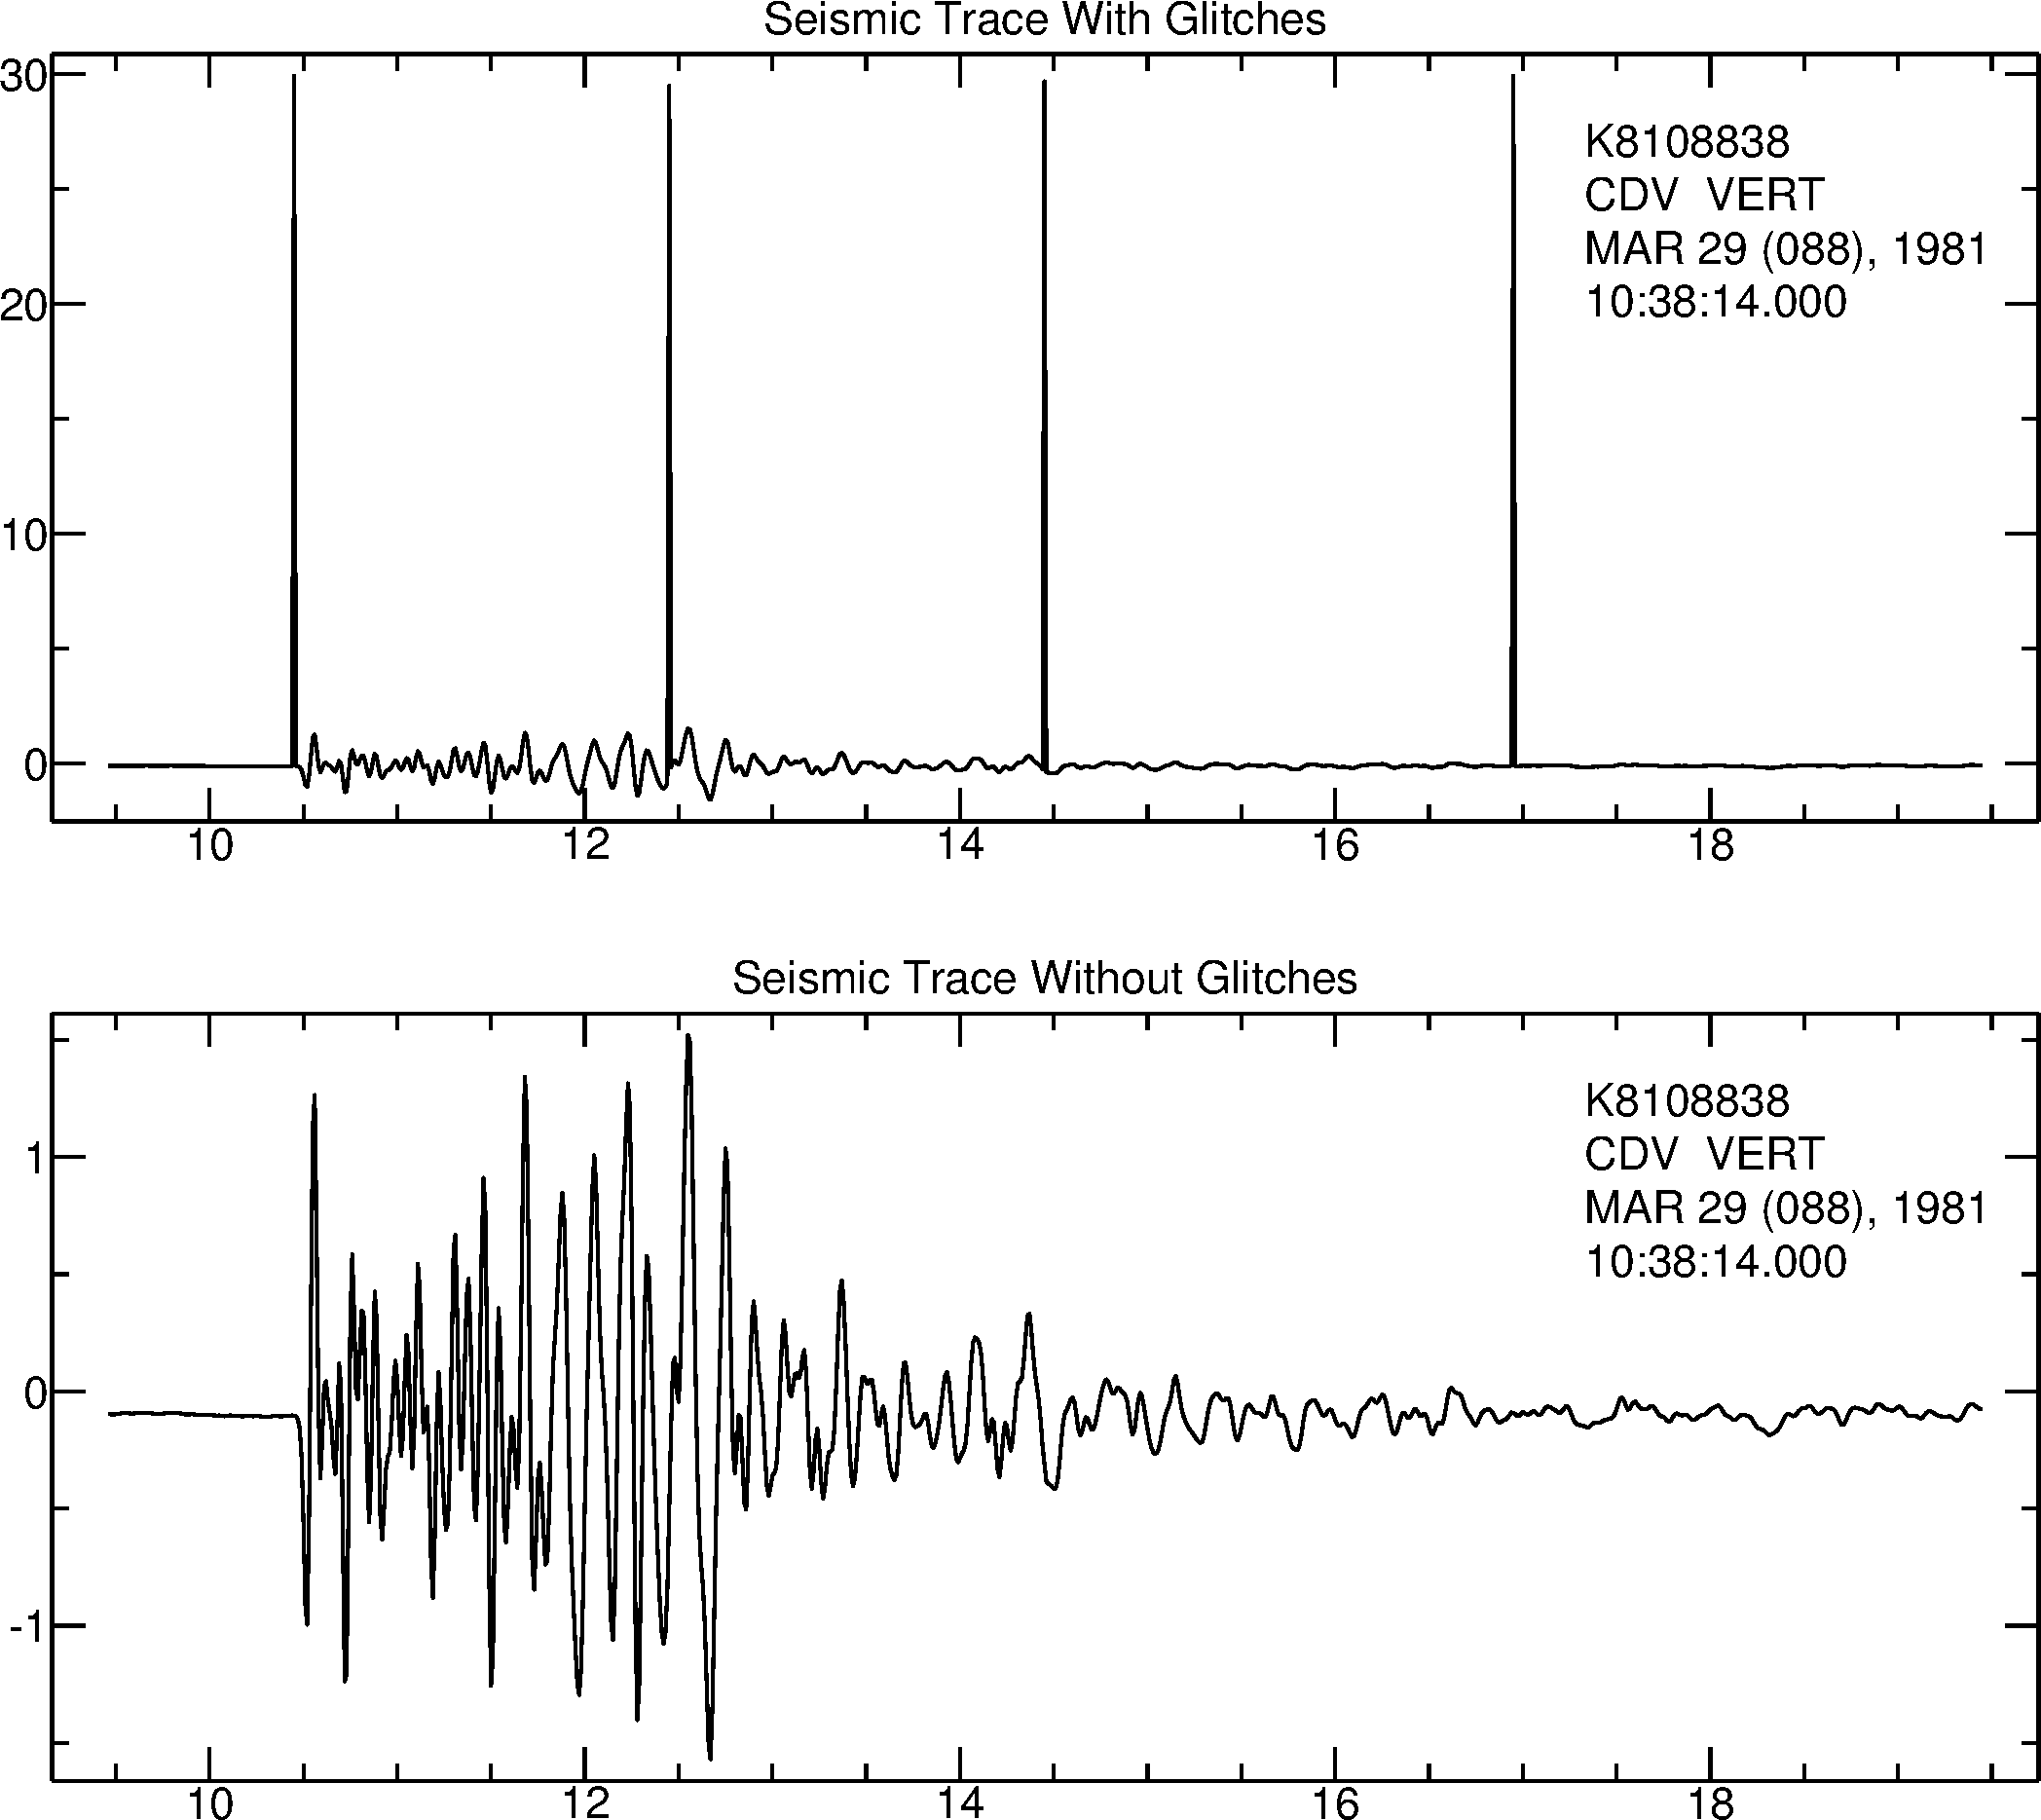
\includegraphics[width=0.95\textwidth]{rglitches}
\caption[地震波形去毛刺]{地震波形去毛刺。上图为包含glitches的地震信号,下图为去除
rglitches后的地震信号。}
\label{fig:deglitches}
\end{figure}

\input{commands/rmean}
\SACCMD{rms}
\label{cmd:rms}

\SACTitle{概要}
计算测量时间窗的信号的均方根

\SACTitle{语法}
\begin{SACSTX}
RMS [NOISE ON|OFF|pdw] [TO USERn]
\end{SACSTX}

\SACTitle{输入}
\begin{description}
\item [NOISE ON] 打开噪声归一化选项
\item [NOISE OFF] 关闭噪声归一化选项
\item [NOISE pdw] 打开噪声归一化选项并改变噪声的部分数据窗。关于pdw,参考\nameref{subsec:pdw}一节。
\item [TO USERn] 定义用于储存结果的头段变量USERn,其中n取0到9
\end{description}

\SACTitle{缺省值}
\begin{SACDFT}
rms noise off to user0
\end{SACDFT}

\SACTitle{说明}
该命令计算当前测量时间窗(参见 \nameref{cmd:mtw})中的数据的均方根。结果写入一个
浮点型头段变量 \texttt{USERn} 中,如果定义了一个噪声时间窗结果可以用于纠正噪声。
计算的一般形式是:对信号窗做一次求和并对可选的噪声窗做另一次求和。

\SACTitle{示例}
为了计算两个头段T1和T2间的数据的未修正的均方根,并将结果保存在头段USER4中:
\begin{SACCode}
SAC> mtw t1 t2
SAC> rms to user4
\end{SACCode}

使用一个5秒长的噪声窗(结束于头段值T3),并就算修正后的均方根:
\begin{SACCode}
SAC> mtw t1 t2
SAC> rms noise t3 -5.0 0.0
\end{SACCode}

\SACTitle{头段变量改变}
USERn

\section{分量旋转}
\label{sec:traces-rotating}
相关命令:\nameref{cmd:rotate}

相关头段:\texttt{cmpinc}、\texttt{cmpaz}

三个正交的地震传感器即可完全记录地面运动矢量。因此可以将三个正交的
分量任意旋转到其它三个正交的方向上。

出于仪器安装的考虑,地震仪三分量一般都是N、E、U向的。而地震学里,
由于SH波与P-SV波的解偶,更常处理的是R、T、Z向的三分量数据。因而地震
信号的旋转是有必要的。

SAC提供了 \nameref{cmd:rotate} 命令,用于旋转任意两个水平分量。
这两个水平分量不需要正交。

\begin{SACCode}
SAC> dg sub teleseis ntkl.[enz]
/opt/sac/aux/datagen/teleseis/ntkl.e ...ntkl.n ...ntkl.z
SAC> w ntkl.e ntkl.n ntkl.z
SAC> r ./ntkl.n ./ntkl.e
SAC> lh cmpinc cmpaz
  FILE: ./ntkl.n - 1
 --------------
     cmpinc = 9.000000e+01
      cmpaz = 0.000000e+00
  FILE: ./ntkl.e - 2
 --------------
     cmpinc = 9.000000e+01
      cmpaz = 9.000000e+01
SAC> rotate to gcp              // 旋转到大圆路径
SAC> lh cmpinc cmpaz
  FILE: ./ntkl.n - 1
 --------------
     cmpinc = 9.000000e+01
      cmpaz = 2.440466e+01
  FILE: ./ntkl.e - 2
 --------------
     cmpinc = 9.000000e+01
      cmpaz = 1.144047e+02
SAC> w ntkl.r ntkl.t            // 保存为R分量和T分量
\end{SACCode}

图 \ref{fig:rotate} 中,左图中从上至下为N、E、Z分量,右图中从上至下
为R、T、Z分量。旋转到R、T分量后,可以很容易地识别出Rayleigh和Love波。

\begin{figure}[H]
\centering
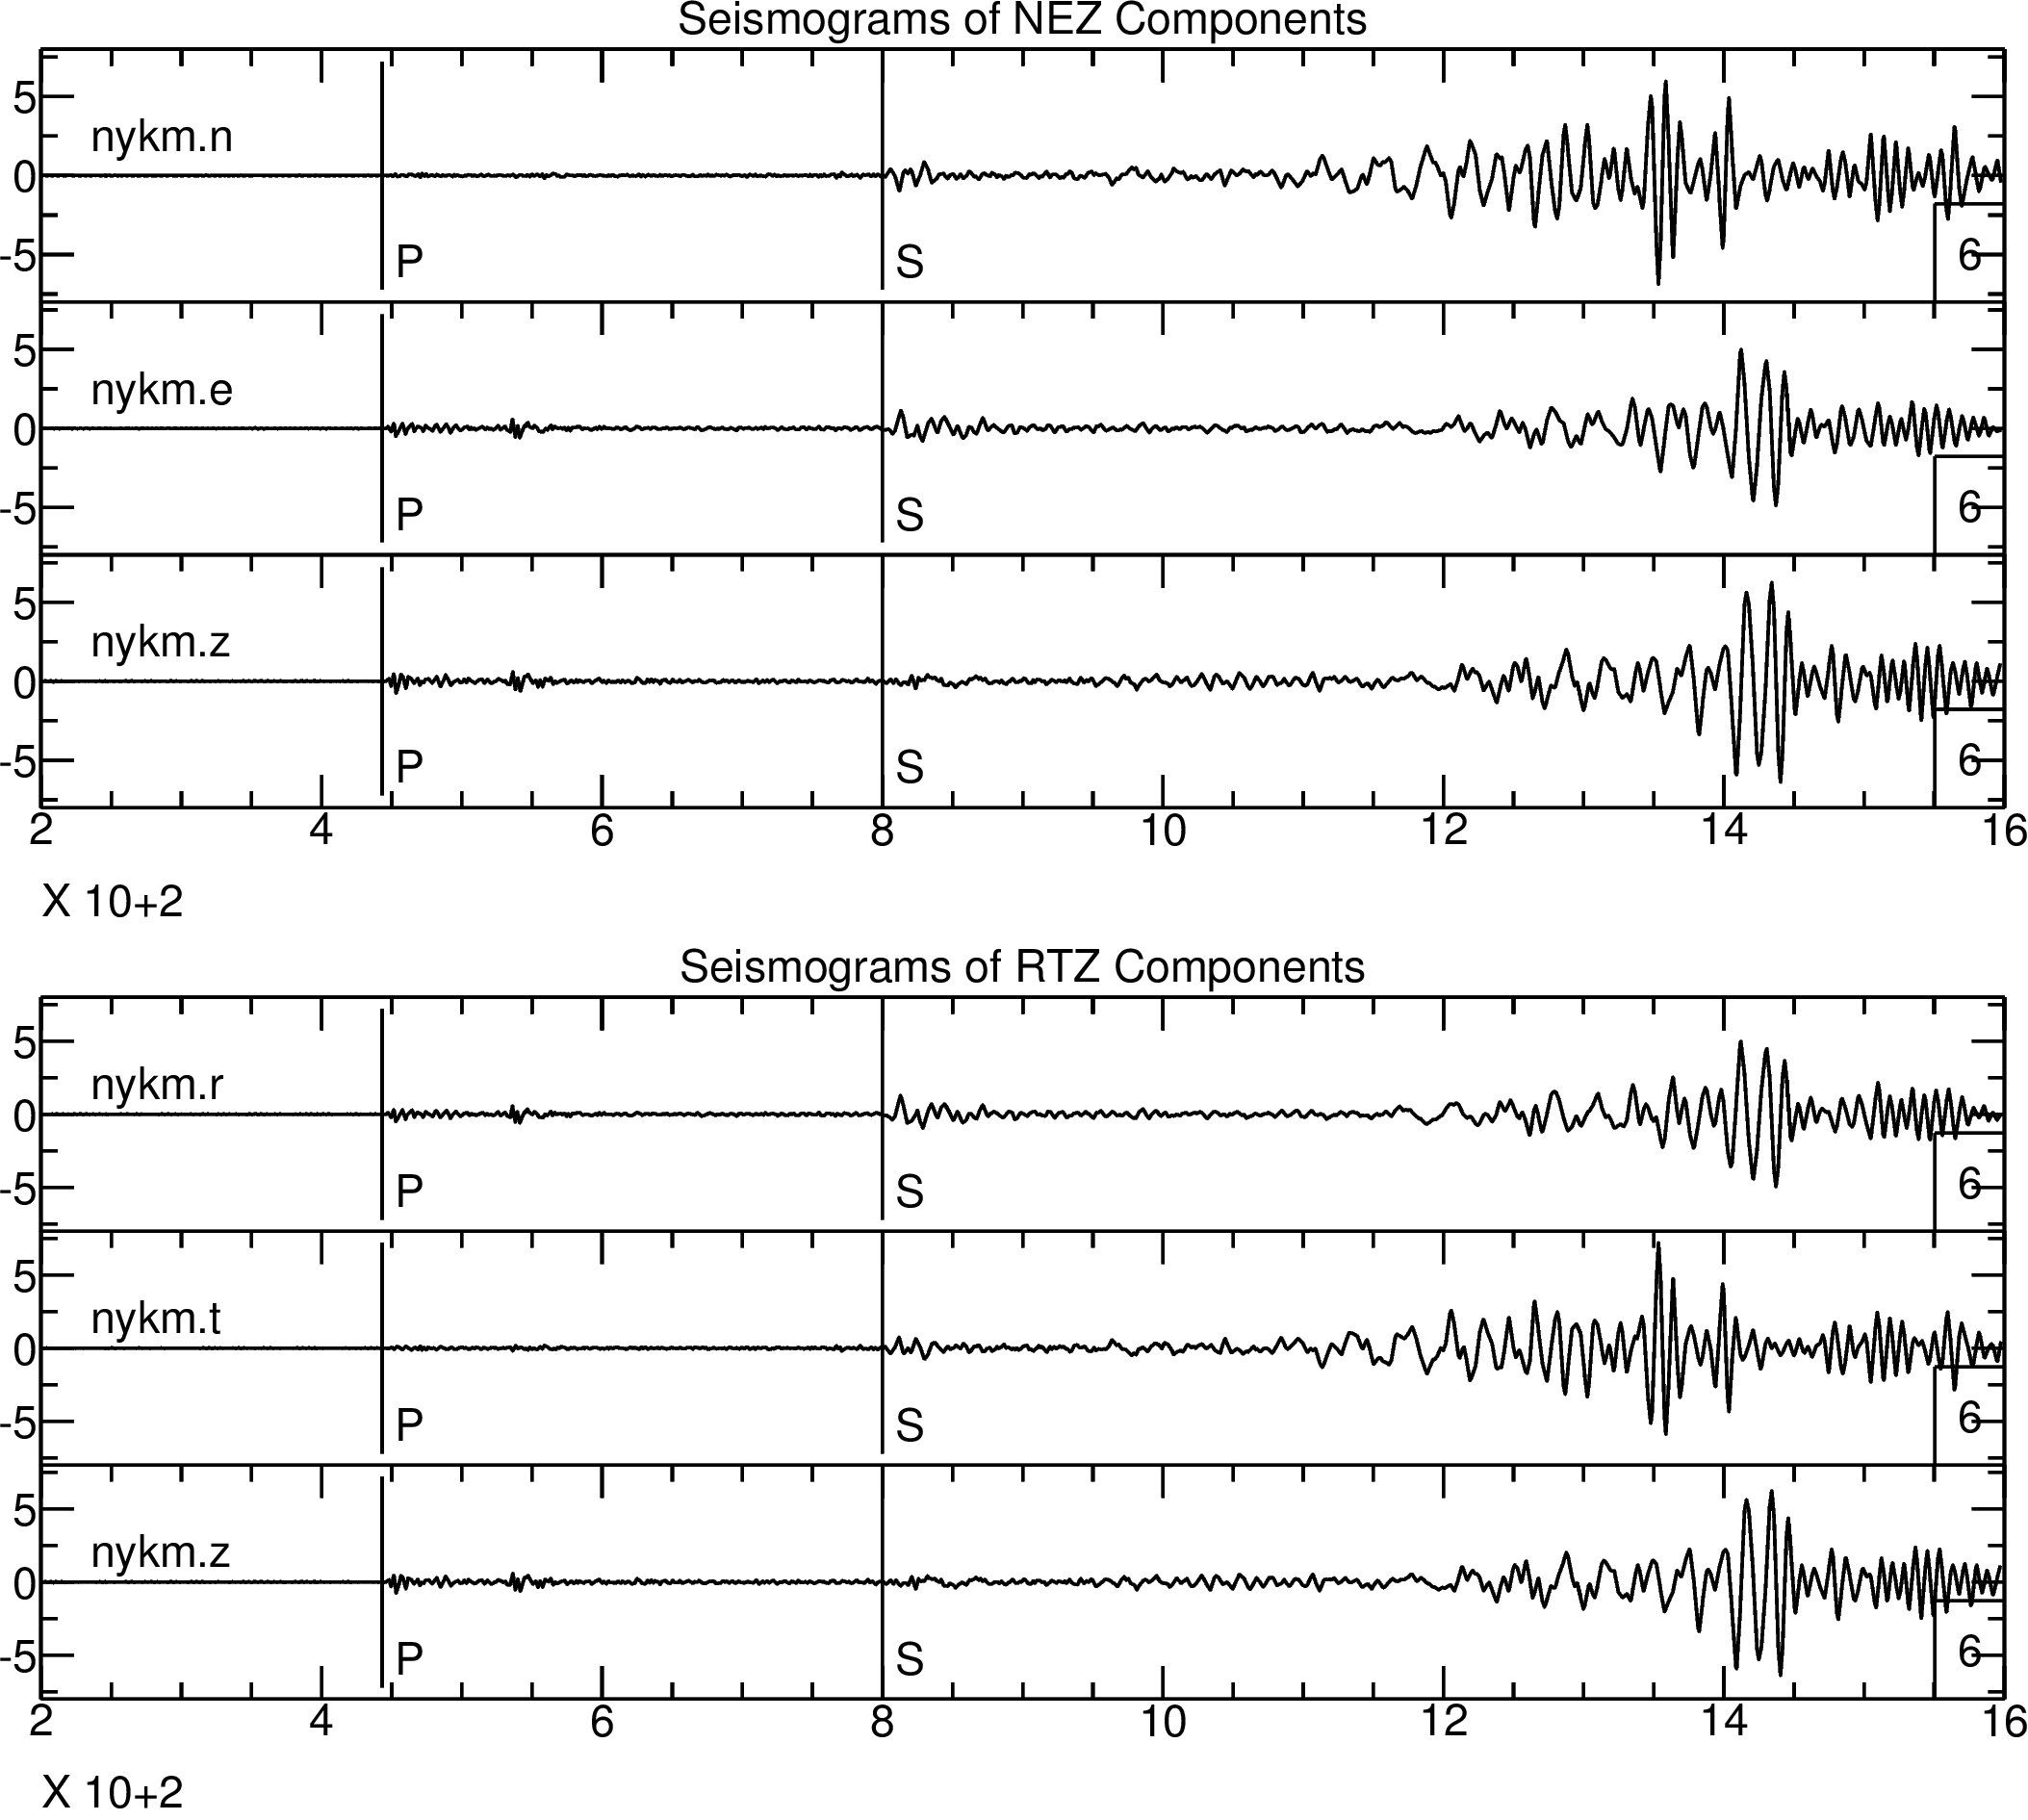
\includegraphics[width=0.95\textwidth]{rotate}
\caption[水平分量旋转]{将N、E分量旋转到R、T分量。}
\label{fig:rotate}
\end{figure}

\SACCMD{rq}
\label{cmd:rq}

\SACTitle{概要}
从谱文件中去除Q因子

\SACTitle{语法}
\begin{SACSTX}
RQ [Q v] [R v] [C v]
\end{SACSTX}

\SACTitle{输入}
\begin{description}
\item [Q v] 设置质量因子为v
\item [R v] 设置距离为v,单位为 \si{\km}
\item [C v] 设置群速度为v,单位 \si{\km\per\s}
\end{description}

\SACTitle{缺省值}
\begin{SACDFT}
rq q 1. r 0. c 1.
\end{SACDFT}

\SACTitle{说明}
该命令用于从波形数据中去除Q衰减效应,用于校正振幅谱的方程如下:
\[ AMP_{corrected}(f) = AMP_{uncorrected}(f) * e^{\frac{\pi R f}{Q C}} \]
其中$f$为频率,单位为 \si{\Hz},$R$为距离,单位 \si{\km},
$C$是群速度,单位为 \si{\km\per\s}。Q是一个无量纲衰减因子。

\SACTitle{头段变量}
depmin、depmax、depmen

\SACTitle{限制}
实际上各参数应是频率的函数,目前限制为常数值。

\SACCMD{rtrend}
\label{cmd:rtrend}

\SACTitle{概要}
去除线性趋势

\SACTitle{语法}
\begin{SACSTX}
RTR!END! [Q!UIET!|!V!ERBOSE]
\end{SACSTX}

\SACTitle{输入}
\begin{description}
\item [QUIET] 不显示线性拟合信息
\item [VERBOSE] 终端显示线性拟合信息
\end{description}

\SACTitle{缺省值}
\begin{SACDFT}
rtrend quiet
\end{SACDFT}

\SACTitle{说明}
该命令利用最小二乘方法将数据拟合成一条直线,然后从数据中减去该直线所
表征的线性趋势。数据可以是不等间隔的。

若有$n$个数据$(x_i,y_i)$,利用最小二乘法拟合直线$y=ax+b$。其中斜率为
\[
    a = \frac{n\sum x_i y_i - \sum x_i \sum y_i}
    {n\sum x_i^2 - (\sum x_i)^2}
\]

Y轴截距为
\[
    b = \frac{\sum x_i^2 \sum y_i - \sum x_i \sum x_i y_i}
    {n\sum x_i^2 - (\sum x_i)^2}
\]

内存中最后一个文件的线性拟合参数将会写入到如下黑板变量中:
\begin{itemize}
\item \verb|RTR_SLP| 直线斜率
\item \verb|RTR_YINT| 直线的Y截距
\item \verb|RTR_SDSLP| 斜率的标准差
\item \verb|RTR_SDYINT| Y截距的标准差
\item \verb|RTR_SDDTA| 数据的标准差
\item \verb|RTR_CORRCF| 数据和拟合结果的相关系数
\end{itemize}

\SACTitle{头段变量改变}
depmin、depmax、depmin

\input{commands/saveimg}
\SACCMD{setbb}
\label{cmd:setbb}

\SACTitle{概要}
设置黑板变量的值

\SACTitle{语法}
\begin{SACSTX}
SETBB variable [APPEND] value [variable [APPEND] value ...]
\end{SACSTX}

\SACTitle{输入}
\begin{description}
\item [variable] 黑板变量名,可以是一个新变量或一个已经有值的变量,
    变量名最长32字符
\item [value] 黑板变量的新值,若包含空格则必须用引号括起来
\item [APPEND] 将值加到变量的旧值之后,若无该选项,则新值将代替旧值
\end{description}

\SACTitle{说明}
\texttt{setbb} 命令可以给黑板变量赋值,这些值可以通过 \nameref{cmd:getbb}
命令获取,或在命令中直接引用。可以使用 \nameref{cmd:evaluate} 对黑板变量
做基本算术操作,并将结果保存在新的黑板变量中,也可以通过 \nameref{cmd:unsetbb}
命令删除一个黑板变量。

\SACTitle{示例}
同时设置多个黑板变量,并在稍后使用使用这些黑板变量:
\begin{SACCode}
SAC> setbb c1 2.45 c2 4.94
SAC> bandpass corners %c1% %c2%
\end{SACCode}

黑板变量的值中包含空格:
\begin{SACCode}
                            // 含空格的值需要用引号括起来
SAC> setbb mytitle 'sample filter response'
SAC> getbb mytitle          // 检查变量值是否正确
 MYTITLE = Sample filter response
SAC> title '%MYTITLE%'      // 引用时需要再次用引用括起来
\end{SACCode}

\SACCMD{setdevice}
\label{cmd:setdevice}

\SACTitle{概要}
定义后续绘图时使用的默认图形设备

\SACTitle{语法}
\begin{SACSTX}
SETDEVICE name
\end{SACSTX}

\SACTitle{输入}
\begin{description}
\item [name] 图形设备名
\end{description}

\SACTitle{说明}
SAC的默认图形设备为X11图形窗口,你可以使用该命令修改默认的图形设备,也可以使用
\nameref{cmd:begindevices} 命令随时用新的图形设备取代默认图形设备。

\SACTitle{相关命令}
\nameref{cmd:begindevices}

\SACCMD{setmacro}
\label{cmd:setmacro}

\SACTitle{概要}
定义SAC宏文件的搜索路径

\SACTitle{语法}
\begin{SACSTX}
SETMACRO [MORE] directory [directory ...]
\end{SACSTX}

\SACTitle{输入}
\begin{description}
\item [directory] 放置SAC宏文件的目录,可以是相对路径或绝对路径
\item [MORE] 将 \texttt{directory} 加到已有的路径列表之后
\end{description}

\SACTitle{说明}
该命令让你能够定义一系列执行宏文件时搜索路径,最多可以定义100个。

当 \texttt{setmacro} 使用 \texttt{more} 选项时,指定的路径会追加到
已存在的路径列表的后面;若没有使用 \texttt{more} 选项,则已存在的列表
将被新列表取代。

当执行 \texttt{macro} 命令时,SAC会先搜索当前目录,若没有找到则搜索
\texttt{setmacro} 指定的目录,若依然没有找到则在全局宏目录中寻找。

\SACCMD{sgf}
\label{cmd:sgf}

\SACTitle{概要}
控制SGF设备选项

\SACTitle{语法}
\begin{SACSTX}
SGF [P!REFIX! text] [N!UMBER! n] [D!IRECTORY! CURRENT|pathname]
    [S!IZE! N!ORMAL!|F!IXED! v|S!CALED! v] [O!VERWRITE! ON|OFF]
\end{SACSTX}

\SACTitle{输入}
\begin{description}
\item [PREFIX text] 设置SGF的文件名前缀为 \texttt{text}(最多24字符长)
\item [NUMBER n] 设置下一个SGF的编号为n。若n为0,则SAC搜索SGF文件
    目录下的SGF文件最大编号,并将其值加1
\item [DIRECTORY CURRENT] 将SGF文件放在当前目录
\item [DIRECTORY pathname] 将SGF放在指定目录下
\item [SIZE NORMAL] 产生一个常规大小绘图,常规图形有一个10*7.5英寸的
    viewspace(最大绘图区域)。viewport(viewspace中除轴和标签之外的、
    绘图区)的默认值为8*5英寸
\item [SIZE FIXED v] 产生一个在X方向viewport为v英寸长的图形
\item [SIZE SCALED v] 产生一个视口在X方向上为v乘以X坐标极限值的图形
\item [OVERWRITE ON|OFF] 当打开时,文件号不递增,每个新文件将擦除先前的
    文件
\end{description}

\SACTitle{缺省值}
\begin{SACDFT}
sgf prefix f number 1 directory current size normal
\end{SACDFT}

\SACTitle{说明}
该命令控制SGF文件的命名规则和后续SGF文件的图形尺寸。SGF文件名由4部分
组成,分别为:
\begin{itemize}
\item \texttt{pathname} 目录路径名,默认为当前目录
\item \texttt{prefix} 前缀,默认值为 \texttt{f}
\item \texttt{number} 三位数的frame编号,默认值为 \texttt{001}
\item \texttt{.sgf} 用于表示SAC图形文件的后缀
\end{itemize}
因而SGF的第一个文件名为 \texttt{f001.sgf}。每次新建一个frame时,frame
编号加1。可以强制frame编号从某个给定的值开始。如果你为准备一个报告需要
工作几天时间,而同时又希望所有图形都按一个统一的顺序排列,那么令frame
编号不从1开始便很有用了。

有多个选项可以控制绘图的尺寸,常规的绘图为10*7.5英寸的veiwport范围,
使用默认的viewport的结果是产生一个近似为8*5英寸的图形区。你可强制viewport
的X方向为固定长度或将viewport的X方向与整个坐标范围成比例。尺寸信息
会被写入SGF文件中,然后由其他转换程序负责将SGF转换成合适大小的图片。

\SACTitle{示例}
设置SGF文件的保存目录为非当前目录,并重置frame编号:
\begin{SACCode}
SAC> sgf dir /mydir/sgfstore frame 0
\end{SACCode}

设置viewport的X方向长度为3英寸:
\begin{SACCode}
SAC> sgf size fixed 3.0
\end{SACCode}

创建一个大小相当于海报的图形:
\begin{SACCode}
SAC> sgf size fixed 30.0
\end{SACCode}

设置vierport的X方向的尺寸与地震数据的时间长度成比例:
\begin{SACCode}
SAC> sgf size scaled 0.1  // 10s的数据长度为1英寸
\end{SACCode}
本例中,持续60秒的数据图形将有6英寸长,而持续600秒的数据将有60英寸长,
过长的图形需要特殊的后期处理。

\SACCMD{smooth}
\label{cmd:smooth}

\SACTitle{概要}
对数据应用算术平滑算法

\SACTitle{语法}
\begin{SACSTX}
SMOOTH [MEAN|MEDIAN] [H!ALFWIDTH! n]
\end{SACSTX}

\SACTitle{输入}
\begin{description}
\item [MEAN|MEDIAN] 应用均值/中值平滑算法
\item [HALFWIDTH n] 设置滑动窗的半宽为n个数据点
\end{description}

\SACTitle{缺省值}
\begin{SACDFT}
smooth mean halfwidth 1
\end{SACDFT}

\SACTitle{说明}
此命令对数据应用算术平滑算法,可以选择均值平滑或中值平滑算法。

滑动窗的窗长通过指定其半宽度n来定义,对于第n到第npts-n+1个的每个数据
点而言,应用一个窗长为$2n+1$个数据点平滑窗。对于两端的$2(n-1$)个数据点而言,
做特殊处理。

\SACTitle{头段变量}
depmin、depmax、depmen

\SACCMD{sonogram}
\label{cmd:sonogram}

\SACTitle{概要}
计算一个频谱图,其等价于同一个谱图的两个不同的平滑版本的差

\SACTitle{语法}
\begin{SACSTX}
SONO!GRAM! [WINDOW v] [SLICE v] [ORDER n] [CBAR ON|OFF]
    [YMIN v] [YMAX v] [FMIN v] [FMAX v] [BINARY|FULL]
    [METHOD PDS|MEM|MLM] [COLOR|GRAY] [PRINT pname]
\end{SACSTX}

\SACTitle{输入}
\begin{description}
\item [WINDOW v] 设置滑动数据窗的长度为v秒,这个窗长决定了FFT的尺寸
\item [SLICE v] 设置数据滑动间隔为v秒,对每个滑动间隔将产生一个频谱图线
\item [ORDER n] 指定用于计算谱估计的自相关中的点数
\item [CBAR ON|OFF] 打开/关闭参考颜色条
\item [BINARY|FULL] 产生一个双色或彩色图像
\item [YMIN v] 指定绘图的最小频率
\item [YMAX v] 指定绘图最大频率
\item [FMIN v] 指定每次滑动频谱图被平滑的最小带宽
\item [FMAX v] 指定每次滑动频谱图被平滑的最大带宽
\item [METHOD PDS|MEM|MLM] 指定使用的谱估计方法,PDS代表功率密度谱估计,MLM代表最大似然,MEM代表最大熵谱估计。
\item [COLOR|GRAY] 指定是彩色图还是灰度图
\end{description}

\SACTitle{缺省值}
\begin{SACDFT}
sonogram window 2 slice 1 method mem order 100 ymin 0 ymax
    fnyquist fmin 2.0 fmax 6.0 full color
\end{SACDFT}

\SACTitle{说明}
sonogram命令计算了一个谱图,其等效于同一谱图两种不同平滑版本的差。依赖于平滑参数fmin和fmax的选择,结果谱图可以加强小幅度谱特性,而其在传统谱图中很难观测到。这个在矿井爆炸的地震信号中寻找高频谱时很有用。(c.f., Hedlin, 1990,Wuster,1993).

\SACTitle{限制}
图形在频率方向的尺寸为512.

\SACTitle{问题}
目前在头段检查以确定他们有相同的分量且在时间上连续方面还有些错误。

\SACTitle{头段变量}
需要:delta

修改:npts、delta、b、e、iftype、depmin、depmax、depmen

创建:nxsize、xminimum、xmaximum、nysize、yminimum、ymaximum

\input{commands/sort}
\SACCMD{spectrogram}
\label{cmd:spectrogram}

\SACTitle{概要}
使用内存中的所有数据计算频谱图

\SACTitle{语法}
\begin{SACSTX}
SP!ECTRO!G!RAM! [WINDOW v] [SLICE v] [ORDER n] [CBAR ON|OFF]
    [SQRT|NLOG|LOG10|NOSCALING]
    [YMIN v] [YMAX v] [METHOD PDS|MEM|MLM] [COLOR|GRAY]
    [PRINT pname]
\end{SACSTX}

\SACTitle{输入}
\begin{description}
\item [WINDOW v] 设置滑动数据窗的长度为v秒,这个窗长决定了FFT的尺寸
\item [SLICE v] 设置数据滑动间隔为v秒,对每个滑动间隔将产生一个频谱图线
\item [ORDER n] 指定用于计算谱估计的自相关中的点数
\item [CBAR ON|OFF] 打开/关闭参考颜色条
\item [SQRT|NLOG|LOG10|NOSCALING] 指定振幅的自然对数、以10为底的对数或平方根
\item [YMIN v] 指定绘图的最小频率
\item [YMAX v] 指定绘图最大频率
\item [METHOD PDS|MEM|MLM] 指定使用的谱估计方法,PDS代表功率密度谱估计,MLM代表最大似然,MEM代表最大熵谱估计。
\item [COLOR|GRAY] 指定是彩色图还是灰度图
\end{description}

\SACTitle{缺省值}
\begin{SACDFT}
spectrogram window 2 slice 1 method mem order 100 noscaling
    ymin 0 ymax fnyquist color
\end{SACDFT}

\SACTitle{说明}
频谱图是通过计算连续并可能重叠的数据时间窗的功率谱并将谱沿着时间轴绘制产生	的。谱是由一个使用MLM或MEM或PDS得到的被截断的自相关函数。一般会选择高精度的MLM和MEM方法,因为他们提高了精度且不会产生由于不同频率之间能量泄漏导致的人工干扰。这些技术的介绍可以参考Kanasewich(1981)以及Lacoss(1971)。被截断的互相关函数的长度由ORDER参数决定。为了保持和spe子程序的一致性,设置了PDS的默认order为200,MEM和MLM的order默认为100。在SAC中每个数据窗的长度由window参数决定。沿着频谱图时间轴的谱之间的间隔由slice参数决定。这两个参数的不同决定了临近时间窗的重叠量,如下图所示:
\begin{SACCode}
Time ->
0  1  2  3  4  5  6  7  8  9 10 11
|.....|.....|.....|.....|.....|.....|.....|.....|.....|.....|..|
|__^__| window 1, First time will be at the center of this window.
      |__^__| window 2
            |__^__| window 3

|.....| Slice: 临近时间窗的开始时间的差
\end{SACCode}
频谱图时间轴的起始和结束点依赖于要被分析的时间序列的长度以及window、slice参数。频谱图的起始时间是时间序列起始时间迟半个窗对应的时间,因为它被定义为第一个窗的中间时刻。SAC不会对数据的前面补0.

\SACTitle{限制}
图形在频率方向的尺寸为512.

\SACTitle{问题}
目前在头段检查以确定他们有相同的分量且在时间上连续方面还有些错误。

\SACTitle{头段变量改变}
需要:delta

改变:npts、delta、b、e、iftype、depmin、depmax、depmen

创建:nxsize、xminimum、xmaximum、nysize、yminimum、ymaximum

\input{commands/sqr}
\input{commands/sqrt}
\input{commands/stretch}
\SACCMD{sub}
\label{cmd:sub}

\SACTitle{概要}
数据文件的每个数据点减去同一个常数

\SACTitle{语法}
\begin{SACSTX}
SUB  [v1 [v2 ... vn]]
\end{SACSTX}

\SACTitle{输入}
\begin{description}
\item [v1] 从第一个文件中减去的常数
\item [v2] 从第二个文件中减去的常数
\item [vn] 从第n个文件中减去的常数
\end{description}

\SACTitle{缺省值}
\begin{SACDFT}
sub 0.0
\end{SACDFT}

\SACTitle{说明}
参见 \nameref{cmd:add} 的相关说明。

\SACTitle{头段变量改变}
depmin、depmax、depmen

\SACCMD{subf}
\label{cmd:subf}

\SACTitle{概要}
使内存中的一组数据减去另一组数据

\SACTitle{语法}
\begin{SACSTX}
SUBF [N!EWHDR! [ON|OFF]] filelist
\end{SACSTX}

\SACTitle{输入}
\begin{description}
\item [NEWHDR ON|OFF] 若为OFF,则生成的数据文件使用内存中原文件的头段;
    若为ON,则生成的数据文件使用filelist中新文件的头段。缺省值为OFF。
\item [filelist] SAC二进制文件列表。
\end{description}

\SACTitle{说明}
参见 \nameref{cmd:addf} 命令的相关说明。

\SACTitle{示例}
参见 \nameref{cmd:addf} 命令的相关示例。

\SACTitle{头段变量}
depmin、depmax、depmen、npts、delta

\SACTitle{相关命令}
\nameref{cmd:read}、\nameref{cmd:binoperr}

\SACCMD{symbol}
\label{cmd:symbol}

\SACTitle{概要}
控制符号绘图属性

\SACTitle{语法}
\begin{SACSTX}
SYM!BOL! [ON|OFF|n] [SIZE v] [SPACING v] [INCRE!MENT! ON|OFF]
    [LIST STANDARD|nlist]
\end{SACSTX}

\SACTitle{输入}
\begin{description}
\item [ON] 打开符号绘图开关,不改变符号号
\item [OFF] 关闭符号绘图开关
\item [n] 打开符号绘图开关。将符号号设置为n。目前有16个不同的符号,符号0意味着关闭符号开关
\item [SIZE v] 设置符号尺寸为v。值为0.01意味着占据整个绘图尺寸的1\%
\item [SPACING v] 设置符号间隔为v。这是绘图时符号间的最小间隔;如果你想每个数据点
    都有符号,则设其值为0,对注释行使用0.2到0.4
\item [INCREMENT ON] 对每个数据文件操作完成后按符号列表递增为下一个符号
\item [INCREMENT OFF] 关闭上述INCREMENT选项
\item [LIST nlist] 改变符号表的内容。输入符号号码表。设置表中的第一个符号码,并打开符号绘图开关
\item [LIST STANDARD] 改变到标准符号表。设置表中的第一个符号表,并打开符号绘制选项。
\end{description}

\SACTitle{缺省值}
\begin{SACDFT}
symbol off size 0.01 spacing 0. increment off list standard
\end{SACDFT}

\SACTitle{说明}
这些符号属性独立于由LINE命令定义的画线属性。打开画线选项,它们也可以用于注释在相同图形上的不同的线。关闭画线选项,则可以绘制散点图。如果你要将几个数据文件画在同一张图上,也许需要使用不同的符号。这是可以使用INCREMENT选项。当这个选项打开时,每次绘制数据文件,都从符号表中将原来的符号码增加1,缺省符号表包含符号表从2到16的符号,你也可以使用LIST选项改变这个表的次序和内容。如果你在绘制一系列重叠绘图,并需要经相同符号用在相同次序的每个图形上,这样做很有用。符号码为0相当于关闭符号绘制选项。这个选项用于LIST选项和LINE选项,以在一张图上用线表示一些数据,用符号表示另外一些数据。

\SACTitle{示例}
为了创建一个散点分布图,关闭画线选项,选择适当的符号,然后绘图:
\begin{SACCode}
SAC> line off
SAC> symbol 5
SAC> plot
\end{SACCode}

为了用符号7、4、6、8注释四条实线,间隔用0.3,用PLOT2绘图:
\begin{SACCode}
SAC> line solid
SAC> sym spacing .3 increment list 7 4 6 8
SAC> r file1 file2 file3 file4
SAC> plot2
\end{SACCode}

使用PLOT2在相同图形上绘制三个文件,第一个文件图形使用实线无符号;第二个没有线,为三角符号;第三个没有线,带有交叉符号:
\begin{SACCode}
SAC> read file1 file2 file3
SAC> line list 1 0 0 increment
SAC> symbol list 0 3 7 increment
SAC> plot2
\end{SACCode}

\SACCMD{synchronize}
\label{cmd:synchronize}

\SACTitle{概要}
同步内存中所有文件的参考时刻

\SACTitle{语法}
\begin{SACSTX}
SYNC!HRONIZE! [R!OUND! ON|OFF] [B!EGIN! ON|OFF]
\end{SACSTX}

\SACTitle{输入}
\begin{description}
\item [ROUND ON] 打开 \texttt{ROUND}选项。若打开该选项,则会对每个文件的
    开始时间做微调以使得开始时间是采样间隔的整数倍
\item [ROUND OFF] 关闭 \texttt{ROUND} 选项
\item [BEGIN ON] 设置每个文件的开始时间为0
\item [BEGIN OFF] 保持参考时间的绝对时刻不变
\end{description}

\SACTitle{缺省值}
\begin{SACDFT}
synchronize round off begin off
\end{SACDFT}

\SACTitle{说明}
该命令用于同步内存中所有文件的参考时刻。通过检查所有文件的参考时间和文件
起始时间(B),找到所有文件中最晚的文件起始时刻,并取该时刻作为内存中
所有文件共同的参考时刻,最后再计算每个文件中所有相对时间相对于新参考时刻
的值。

当数据文件具有不同的参考时刻时,对数据使用 \nameref{cmd:cut} 或 \nameref{cmd:xlim}
命令就会有些麻烦,因而可以使用该命令使得所有数据的参考时刻一致。

如果使用了 \texttt{BEGIN} 选项,则会将所有文件的 \texttt{kzdate} 和
\texttt{kztime} 设置为同样的值,并将所有文件的开始时间(B)设置为零,
这样做会使得数据丢失绝对时间信息。

\SACTitle{示例}
假定你读取两个不同参考时间的文件到内存:
\begin{SACCode}
SAC> read file1 file2
SAC> listhdr b kztime kzdate

  FILE: FILE1
  -
  B = 0.
  KZTIME = 10:38:14.000
  KZDATE = MAR 29 (088), 1981

  FILE: FILE2
  -
  B = 10.00
  KZTIME = 10:40:10.000
  KZDATE = MAR 29 (088), 1981
\end{SACCode}

这些文件有相同的参考日期,不同的参考时刻以及不同的开始时间偏移量。可以
执行 \texttt{synchronize} 同步参考时刻:
\begin{SACCode}
SAC> synchronize
SAC> listhdr

  FILE: FILE1
  -
  B = -126.00
  KZTIME = 10:40:20.000
  KZDATE = MAR 29 (088), 1981

  FILE: FILE2
  -
  B = 0.
  KZTIME = 10:40:20.000
  KZDATE = MAR 29 (088), 1981
\end{SACCode}
现在内存中的所有文件有相同的参考时间,如果头段中有任何已定义的时间标记,
它们的值也会调整以保证其绝对时刻是不变的。

\SACCMD{systemcommand}
\label{cmd:systemcommand}

\SACTitle{概要}
在SAC内部执行系统命令

\SACTitle{语法}
\begin{SACSTX}
S!YSTEM!C!OMMAND! command [ options ]
\end{SACSTX}

\SACTitle{输入}
\begin{description}
\item [command] 系统命令名
\item [options] 命令需要的选项
\end{description}

\SACTitle{说明}
在SAC中是可以执行大部分系统命令的,比如常见的 \texttt{ls}、\texttt{cp} 等。

但是某些命令无法直接在SAC中执行,比如用于查看PS文件的gs命令会首先被SAC解释为
\nameref{cmd:grayscale} 的简写,故而在SAC中无法直接调用gs命令。

另一个经常使用但无法直接调用的命令是 \texttt{rm}。由于 \nameref{cmd:read} 命令
可以被简写为 \texttt{r} ,在读入文件时键入 \texttt{r *.SAC} 很可能会一时手误
敲成 \texttt{rm *.SAC} ,为了避免类似的误操作,故而在SAC中禁止直接调用 \texttt{rm} 命令。

当需要在SAC内部执行删除命令时,则需要使用 \nameref{cmd:systemcommand} 调用系统命令。

\SACTitle{示例}
调用系统命令删除某些SAC文件:
\begin{SACCode}
SAC> rm junks
 ERROR 1106: Not a valid SAC command.
SAC> sc rm junks
\end{SACCode}
\SACCMD{taper}
\label{cmd:taper}

\SACTitle{概要}
对数据两端应用对称的taper函数,使得数据两端平滑地衰减到零

\SACTitle{语法}
\begin{SACSTX}
TAPER [T!YPE! HAN!NING!|HAM!MING!|C!OSINE!] [W!IDTH! v]
\end{SACSTX}

\SACTitle{输入}
\begin{description}
\item [TYPE HANNING|HAMMIN|COSINE] 应用Hanning、Hamming、余弦衰减窗
\item [WIDTH v] 设置衰减窗的宽度占数据总点数(npts)的比值为v,v取值在0.0和0.5之间
\end{description}

\SACTitle{缺省值}
\begin{SACDFT}
taper type hanning width 0.05
\end{SACDFT}

\SACTitle{说明}
taper函数是在0和1之间取值的单调函数,若将其对称地施加于数据的首尾两端,则可实现
数据的``尖灭''。

taper函数共计$npts*v$个点,第一个点值为0,最后一个点的值为1,将此函数的每个点依次
于数据的第1至$npts*v$个点相乘,使得数据数据的首端从0开始光滑地增加到其原始值。
数据的末端完全类似,此时数据由其原始值不断光滑地减小到0。

taper命令的通用形式为
\[
    Data(j) = Data(j)*(F_0 - F_1\cos(\omega(j-1)))
\]
此公式应用于数据的首端,另一个完全对称的数据用于数据的尾端。

表 \ref{table:taper-functions} 定义了不同的衰减函数的参数,其中N为衰减窗的宽度,即$npts*v$。
\begin{table}[ht]
\centering
\caption{taper衰减函数参数一览}
\label{table:taper-functions}
\begin{tabular}{llll}
\toprule
类型 & $\omega$ & $F_0$	& $F_1$	\\
\midrule
HANNING	&	$\frac{\pi}{N}$	&	0.50	&	0.50	\\
HAMMING	&	$\frac{\pi}{N}$	&	0.54	&	0.46	\\
COSINE	&	$\frac{\pi}{2N}$	&	1.00	&	1.00	\\
\bottomrule
\end{tabular}
\end{table}

图 \ref{fig:taper-functions} 给出了不同taper衰减函数的曲线图,图中可以看出,HAMMING
窗实际上并没有完全实现尖灭。
\begin{figure}[!ht]
\centering
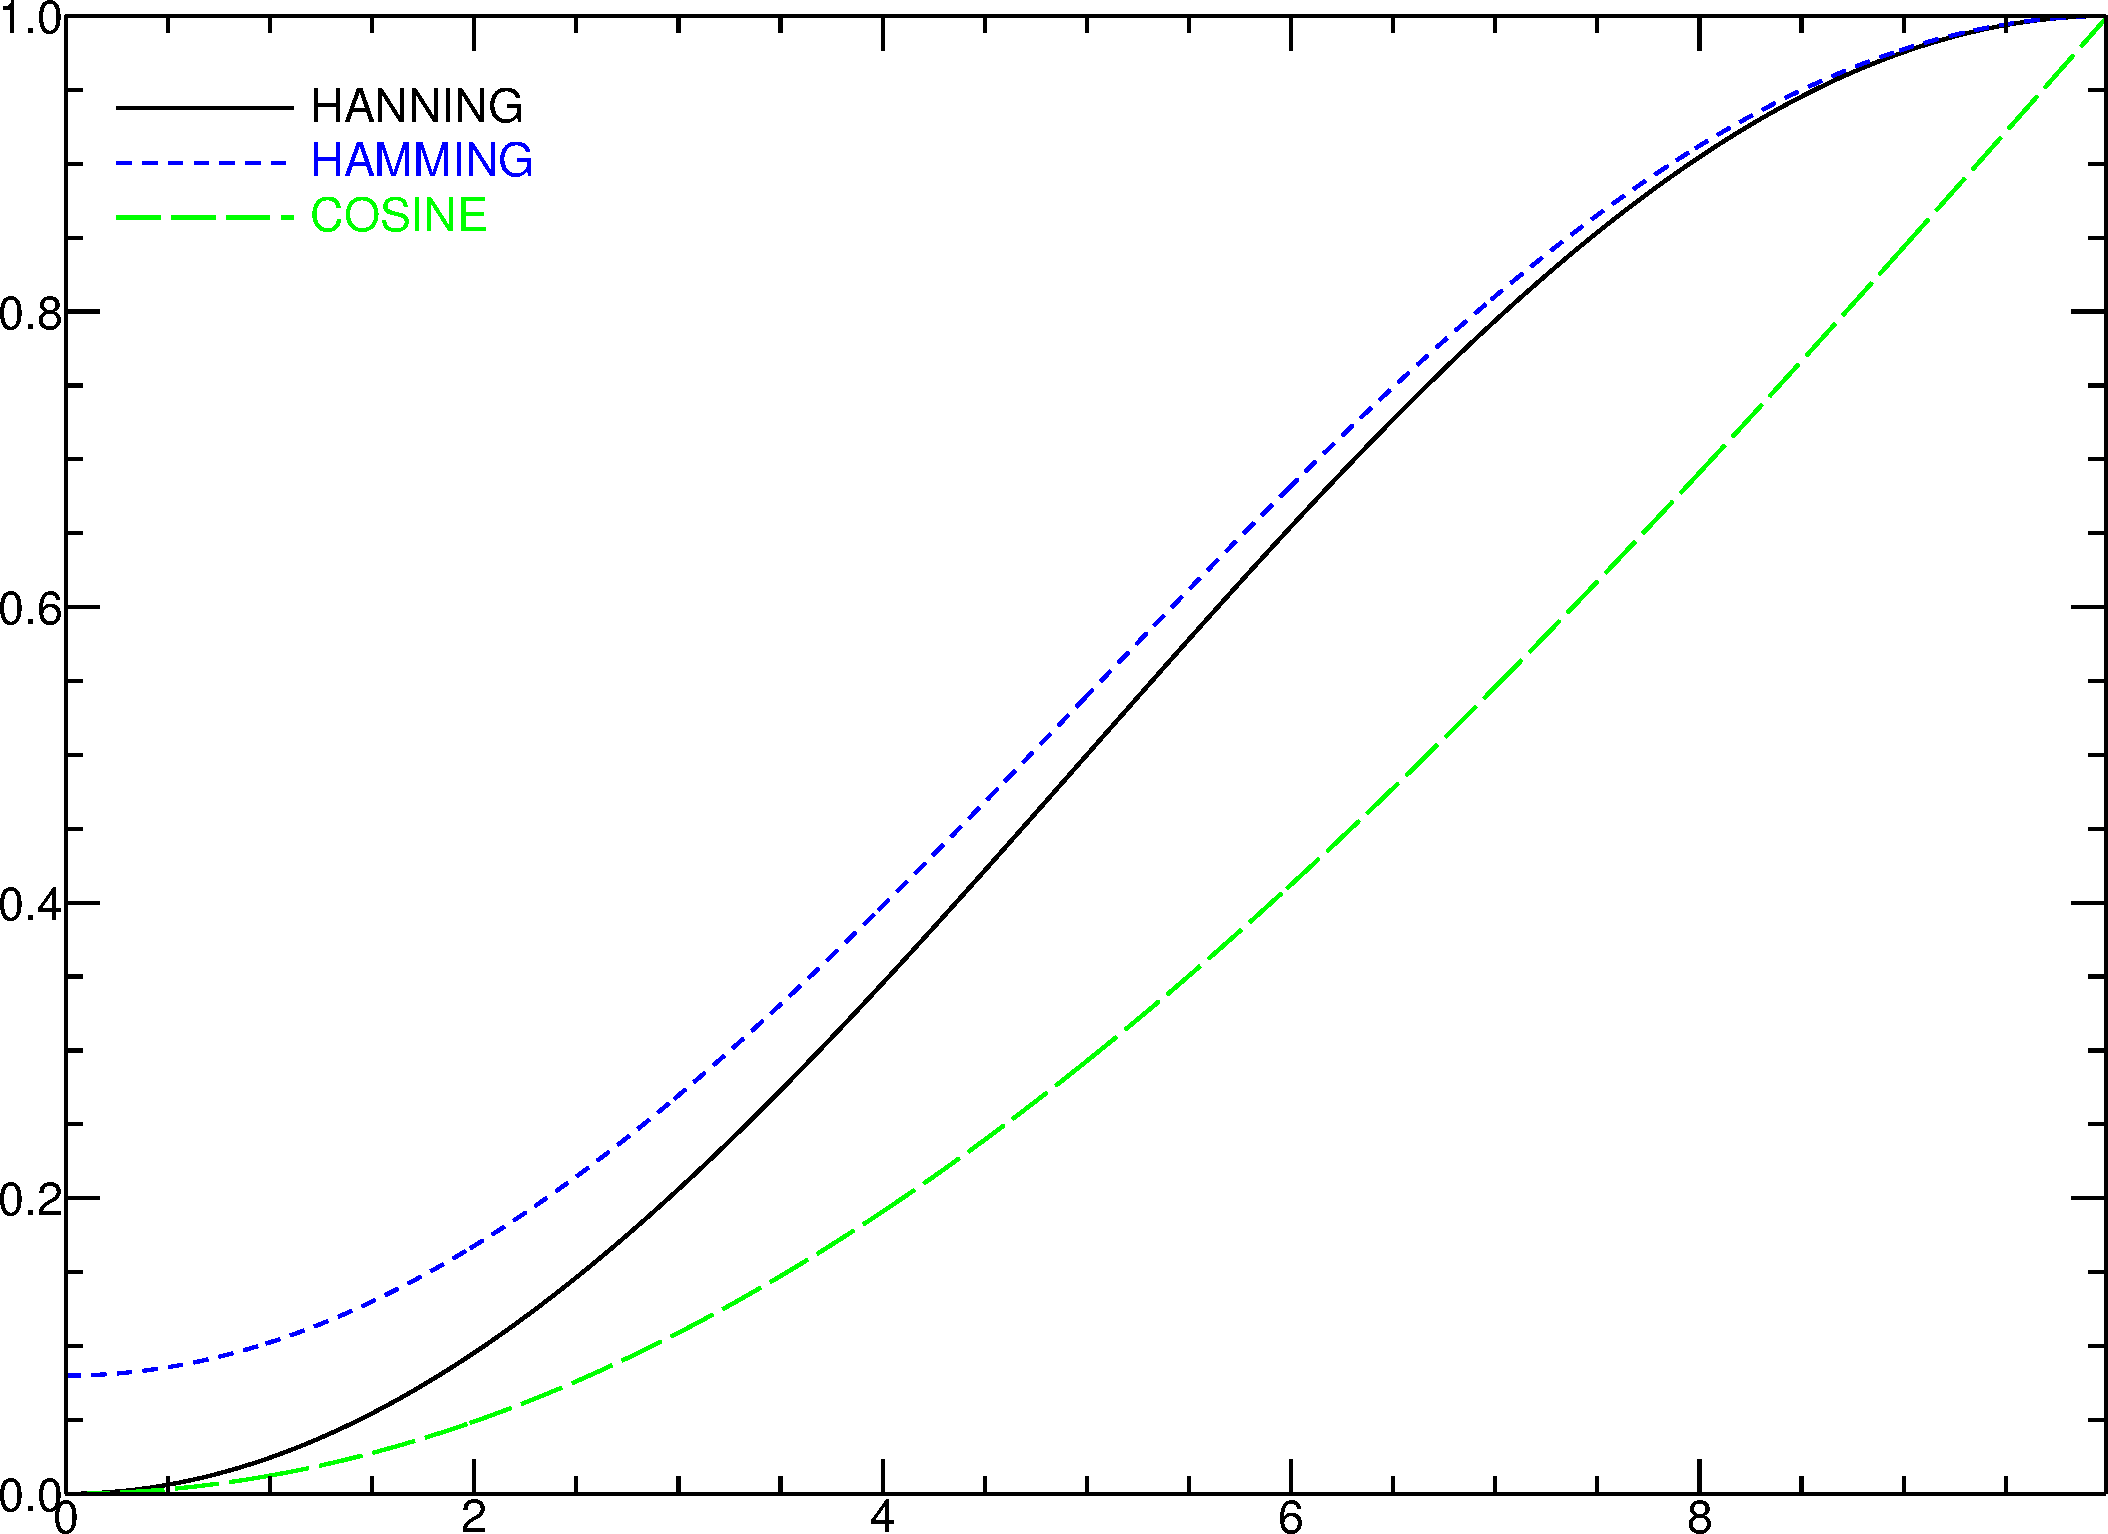
\includegraphics[width=0.8\textwidth]{taper-functions}
\caption{taper衰减函数曲线}
\label{fig:taper-functions}
\end{figure}

\SACTitle{头段变量}
depmin、depmax、depmen

\SACCMD{ticks}
\label{cmd:ticks}

\SACTitle{概要}
控制绘图上刻度轴的位置

\SACTitle{语法}
\begin{SACSTX}
TICKS [ON|OFF|ONLY] [A!LL!] [T!OP!] [B!OTTOM!] [R!IGHT!] [L!EFT!]
\end{SACSTX}

\SACTitle{输入}
\begin{description}
\item [ON] 在指定的边上显示刻度,其他不变
\item [OFF] 在指定的边上不显示刻度,其他不变
\item [ONLY] 仅在指定的边上显示刻度,其他关闭
\item [ALL] 所有四条边
\item [TOP] 视口上部的X轴
\item [BOTTOM] 视口的下部的X轴
\item [RIGHT] 视口右边的Y轴
\item [LEFT] 视口左边的Y轴
\end{description}

\SACTitle{缺省值}
\begin{SACDFT}
ticks on all
\end{SACDFT}

\SACTitle{说明}
刻度轴可以画图形四边的一边或几边上,刻度间隔由 \nameref{cmd:xdiv} 命令控制。

\SACTitle{示例}
显示上部刻度轴,其他不变:
\begin{SACCode}
SAC> ticks on top
\end{SACCode}

关闭所有刻度轴:
\begin{SACCode}
SAC> ticks off all
\end{SACCode}

显示底部刻度轴,其余关闭:
\begin{SACCode}
SAC> ticks only bottom
\end{SACCode}

\SACCMD{title}
\label{cmd:title}

\SACTitle{概要}
定义绘图的标题和属性

\SACTitle{语法}
\begin{SACSTX}
TITLE [ON|OFF|text] [L!OCATION! T!OP!|B!OTTOM!|R!IGHT!|L!EFT!]
    [S!IZE! T!INY!|S!MALL!|M!EDIUM!|L!ARGE!]
\end{SACSTX}

\SACTitle{输入}
\begin{description}
\item [ON] 显示标题,但不改变标题内容
\item [OFF] 不显示标题
\item [text] 显示标题,并改变标题内容。如果文本中包含空格,则标题需要用单引号括起来
\item [LOCATION] 设置标题的位置,可以取TOP、BOTTOM、RIGHT、LEFT
\item [SIZE] 设置标题文本尺寸,可以取TINY、SMALL、MEDIUM、LARGE
\end{description}

\SACTitle{缺省值}
\begin{SACDFT}
title off location top size small
\end{SACDFT}

\SACTitle{说明}
若打开该选项,则在每个图形上都显示标题,标题的尺寸、位置及内容均可改变,文本质量和
字体可以通过 \nameref{cmd:gtext} 命令设置。

\SACTitle{相关命令}
\nameref{cmd:gtext}

\SACCMD{trace}
\label{cmd:trace}

\SACTitle{概要}
追踪黑板变量和头段变量

\SACTitle{语法}
\begin{SACSTX}
TRACE [ON|OFF] name [name ...]
\end{SACSTX}

\SACTitle{输入}
\begin{description}
\item [ON] 打开变量追踪选项
\item [OFF] 关闭变量追踪选项
\item [name] 要追踪的黑板变量或/和头段变量名。对于头段变量,其格式为\texttt{filename,hdrname} ,
    其中filename是要追踪的SAC文件名或文件号,hdrname是SAC头段变量名。
\end{description}

\SACTitle{缺省值}
\begin{SACDFT}
trace on
\end{SACDFT}

\SACTitle{说明}
该命令用于在SAC执行过程中追踪SAC黑板变量或/和头段变量的值,主要用于调试大型或复杂的宏文件。
当变量追踪选项被打开时,将显示变量的当前值。若变量追踪选项处于打开状态,则每次执行命令时将
对变量值进行检查,若变量的值发生改变则将其新值打印到终端。当变量追踪选项被关闭时,也会显示
变量的当前值。

\SACTitle{示例}
追踪黑板变量TEMP1和文件MYFILE的头段变量T0:
\begin{SACCode}
SAC> trace on temp1 myfile,t0
  TRACE  (on) TEMP1 = 1.45623
  TRACE  (on) MYFILE,T0 = UNDEFINED
\end{SACCode}

在执行命令时,SAC会检查变量值是否发生改变。若发生改变则将相关信息显示出来。假设在完成一些计算之后
改变了TEMP1,并定义了T0的值,则SAC将显示如下信息:
\begin{SACCode}
  TRACE (mod) TEMP1 = 2.34293
  TRACE (mod) MYFILE,T0 = 10.3451
\end{SACCode}

稍后的处理中TEMP1可能再次改变:
\begin{SACCode}
  TRACE (mod) TEMP1 = 1.93242
\end{SACCode}

当跟踪选项被关闭时,SAC最后一次显示变量当前值:
\begin{SACCode}
SAC> trace off temp1 myfile,t0
  TRACE (off) TEMP1 = 1.93242
  TRACE (off) MYFILE,T0 = 10.3451
\end{SACCode}

\SACCMD{transcript}
\label{cmd:transcript}

\SACTitle{概要}
控制输出到副本文件

\SACTitle{语法}
\begin{SACSTX}
TRANSCRIPT [OPEN|CREATE|CLOSE|CHANGE|WRITE|HISTORY] [FILE filename]
    [CONTENTS ALL|ERRORS|WARNINGS|OUTPUT|COMMANDS|MACROS|PROCESSED]
    [MESSAGE text]
\end{SACSTX}

\SACTitle{输入}
\begin{description}
\item [OPEN] 打开副本文件,并在已存在的文件底部添加副本
\item [CREATE] 创建一个新的副本文件
\item [CLOSE] 关闭一个已经打开的副本文件
\item [CHANGE] 改变一个已经打开的副本文件的内容
\item [WRITE] 写信息到一个副本文件,不改变其状态或内容
\item [HISTORY FILE filename] 将命令行历史保存到文件
\item [FILE filename] 定义副本文件的名字
\item [MESSAGE text] 向副本文件中写入文本。这个信息可以用于指定正在进行的
    进程或指定正在处理的不同事件,在两次执行这个命令的过程中这个信息不保存
\item [CONTENTS ALL] 定义副本文件的内容为全部输入输出的信息
\item [CONTENTS list] 定义副本文件的内容,即包含在文件中的输入输出的类型表
\end{description}
其中 \texttt{list} 可以取:
\begin{itemize}
\item \texttt{ERRORS}:执行命令期间产生的错误消息
\item \texttt{WARNINGS}:执行命令期间产生的警告消息
\item \texttt{OUTPUT}:执行命令期间的输出消息
\item \texttt{COMMANDS}:终端输出的原始命令
\item \texttt{MACROS}:宏文件中出现的原始命令
\item \texttt{PROCESSED}:经终端或宏处理之后的命令
\end{itemize}

\SACTitle{缺省值}
\begin{SACDFT}
transcript open file transcript contents all
\end{SACDFT}

\SACTitle{说明}
副本文件用于记录SAC执行的结果。其可以是一个完整或部分副本,可以包含一次
或多次执行的结果。你可以同时拥有5个活动的副本文件,每个文件用于追踪不同
的方面。其中的一个用途是记录终端输入的命令然后用于一个宏文件中,如下例所示。

\SACTitle{示例}
为了创建一个新的副本文件,文件名为mytran,包含了除已处理命令之外的其他
全部类型:
\begin{SACCode}
SAC> transcript create file mytran cont err warn out com macros
\end{SACCode}

如果之后不想把宏命令送入这个文件,你可以使用 \texttt{CHANGE} 选项:
\begin{SACCode}
SAC> transcript change file mytran contents e w o c
\end{SACCode}

为了定义一个名为myrecord的副本文件,其记录了终端输入的命令:
\begin{SACCode}
SAC> transcript create file myrecord contents commands
\end{SACCode}

以后,经过适当的编辑,这个文件可以用作宏命令文件,去自动执行相同的一组
命令。在最后的例子中假设你需要彻夜处理许多事件。你可以设置每个事件一个
副本文件(用不同的副本文件名)去记录处理的结果。另外你可以将处理所有事件
得到的任何错误消息保存到一个副本文件中:
\begin{SACCode}
SAC> transcript open file errortran contents errors
SAC> transcript write message 'processing event 1'
\end{SACCode}

这些命令将放在处理每个事件的宏文件中,它假设事件名作为第一个参数带入宏。
使用打开选项,运行信息和出错信息将添加到文件的后面,第二天检查一下这个
出错信息副本文件,就可以快速查阅在处理期间是否出现了错误。

为了将保存一个命令行副本,以记录SAC当前和将来要运行的命令:
\begin{SACCode}
SCA> transcript history file .sachist
\end{SACCode}
这就在当前目录创建并写入了一个副本文件``\verb|~/.sachist|''。任何储存在
那里的文件将被载入命令历史中。如果这个命令位于你的启动初始化宏文件中,
则每次你运行SAC时将在当前目录产生一个单独的命令行历史。在一个新执行的SAC中,
上下键将浏览完整的命令历史,你可以修改以前输入的命令并再次执行它,如果你
没有在SAC内或初始化宏文件中输入这个命令,则命令行历史将自动保存到
\verb|~/.sac_history|。

\SACCMD{transfer}
\label{cmd:transfer}

\SACTitle{概要}
反卷积以去除仪器响应,如果需要,还可以卷积其他仪器响应

\SACTitle{语法}
\begin{SACSTX}
TRANS!FER! [FROM type [options]] [TO type [options]]
    [FREQ!LIMITS! f1 f2 f3 f4] [PREWH!ITENING! ON|OFF|n]
\end{SACSTX}

\SACTitle{输入}
\begin{description}
\item [FROM type] 要去除的仪器响应类型;
\item [TO type] 要加入的仪器响应类型;
\item [FREQLIMITS f1 f2 f3 f4] 压制大于f4以及低于f1的频段;
\item [PREWHITENING ON|OFF|n] 预白化处理。
\end{description}

\SACTitle{缺省值}
\begin{SACDFT}
trans from none to none
\end{SACDFT}

\SACTitle{说明}
\subsubsection{FROM and TO}
transfer命令的作用是将波形数据从一种仪器响应转换成另一种仪器响应。
\texttt{FROM type} 指定要从波形数据中去除的仪器响应,\texttt{TO type} 指定了要加入
到波形数据中的仪器响应。去仪器响应即反卷积,加仪器响应即卷积,二者分别通过
谱域的除法和乘法完成。

\texttt{type} 为仪器类型,可以是SAC预定义的标准仪器类型
(见附录中表 \ref{table:instrument-type}),还可以是如下几种特殊的``仪器类型'':
\begin{description}
\item [none] 表示``位移''
\item [vel] 表示``速度''
\item [acc] 表示``加速度''
\item [evalresp] 表示使用RESP仪器响应文件
\item [polezero] 表示使用SAC PZ仪器响应文件
\item [fap] 表示使用fap仪器响应文件
\end{description}

tranfser命令的默认值是``\texttt{transfer from none to none}'',即默认的输入和
输出``仪器''都是位移。因而当不指定 \texttt{FROM type} 或 \texttt{TO type} 时,SAC
会假定仪器类型为 \texttt{NONE}。

\begin{itemize}
\item 若输出的仪器类型为 \texttt{NONE},即表示从波形中去除仪器响应得到位移,
    此时SAC头段中的IDEP设置为 \texttt{IDISP},单位为 \texttt{nm},若输出类型为
    \texttt{VEL} 或 \texttt{ACC},同理;
\item 若输出的仪器类型不是 \texttt{NONE}、\texttt{VEL} 或 \texttt{ACC},则内存中的波形会
    卷积上 \texttt{TO type} 所指定的仪器响应;
\item 若不指定 \texttt{FROM} 选项,则假定原始波形数据是位移,且不会去除仪器响应;通常
    用于给理论地震图添加仪器响应;
\end{itemize}

\subsubsection{freqlimits}
freqlimits用于在去除仪器响应时对波形的低频和高频部分进行压制。当 \texttt{TO type} 为
NONE、VEL或ACC时,必须使用该选项,且必须认真选择合适的参数。

所有地震仪在零频率处都具有零响应,在只进行反卷积时,需要在频率域做谱的除法,此时
可能会除以一个很小的值进而导致低频处有很大的谱振幅;在高频处,信噪比通常很低,
因而有必要对其响应进行压制。

freqlimits会在去仪器响应时对频谱做低通和高通尖灭,以实现对高频和低频的压制。
四个频率参数应满足 \texttt{f1<f2<f3<f4},即尖灭函数在零到f1之间为0,f1到f2之间
从0渐渐变成1,在f2和f3之间保持为1,在f3到f4之间从1渐渐变成0,大于f4的频段
值为0。过渡带内分别为余弦波的四分之一周期。如下图所示:

\begin{figure}[H]
\centering
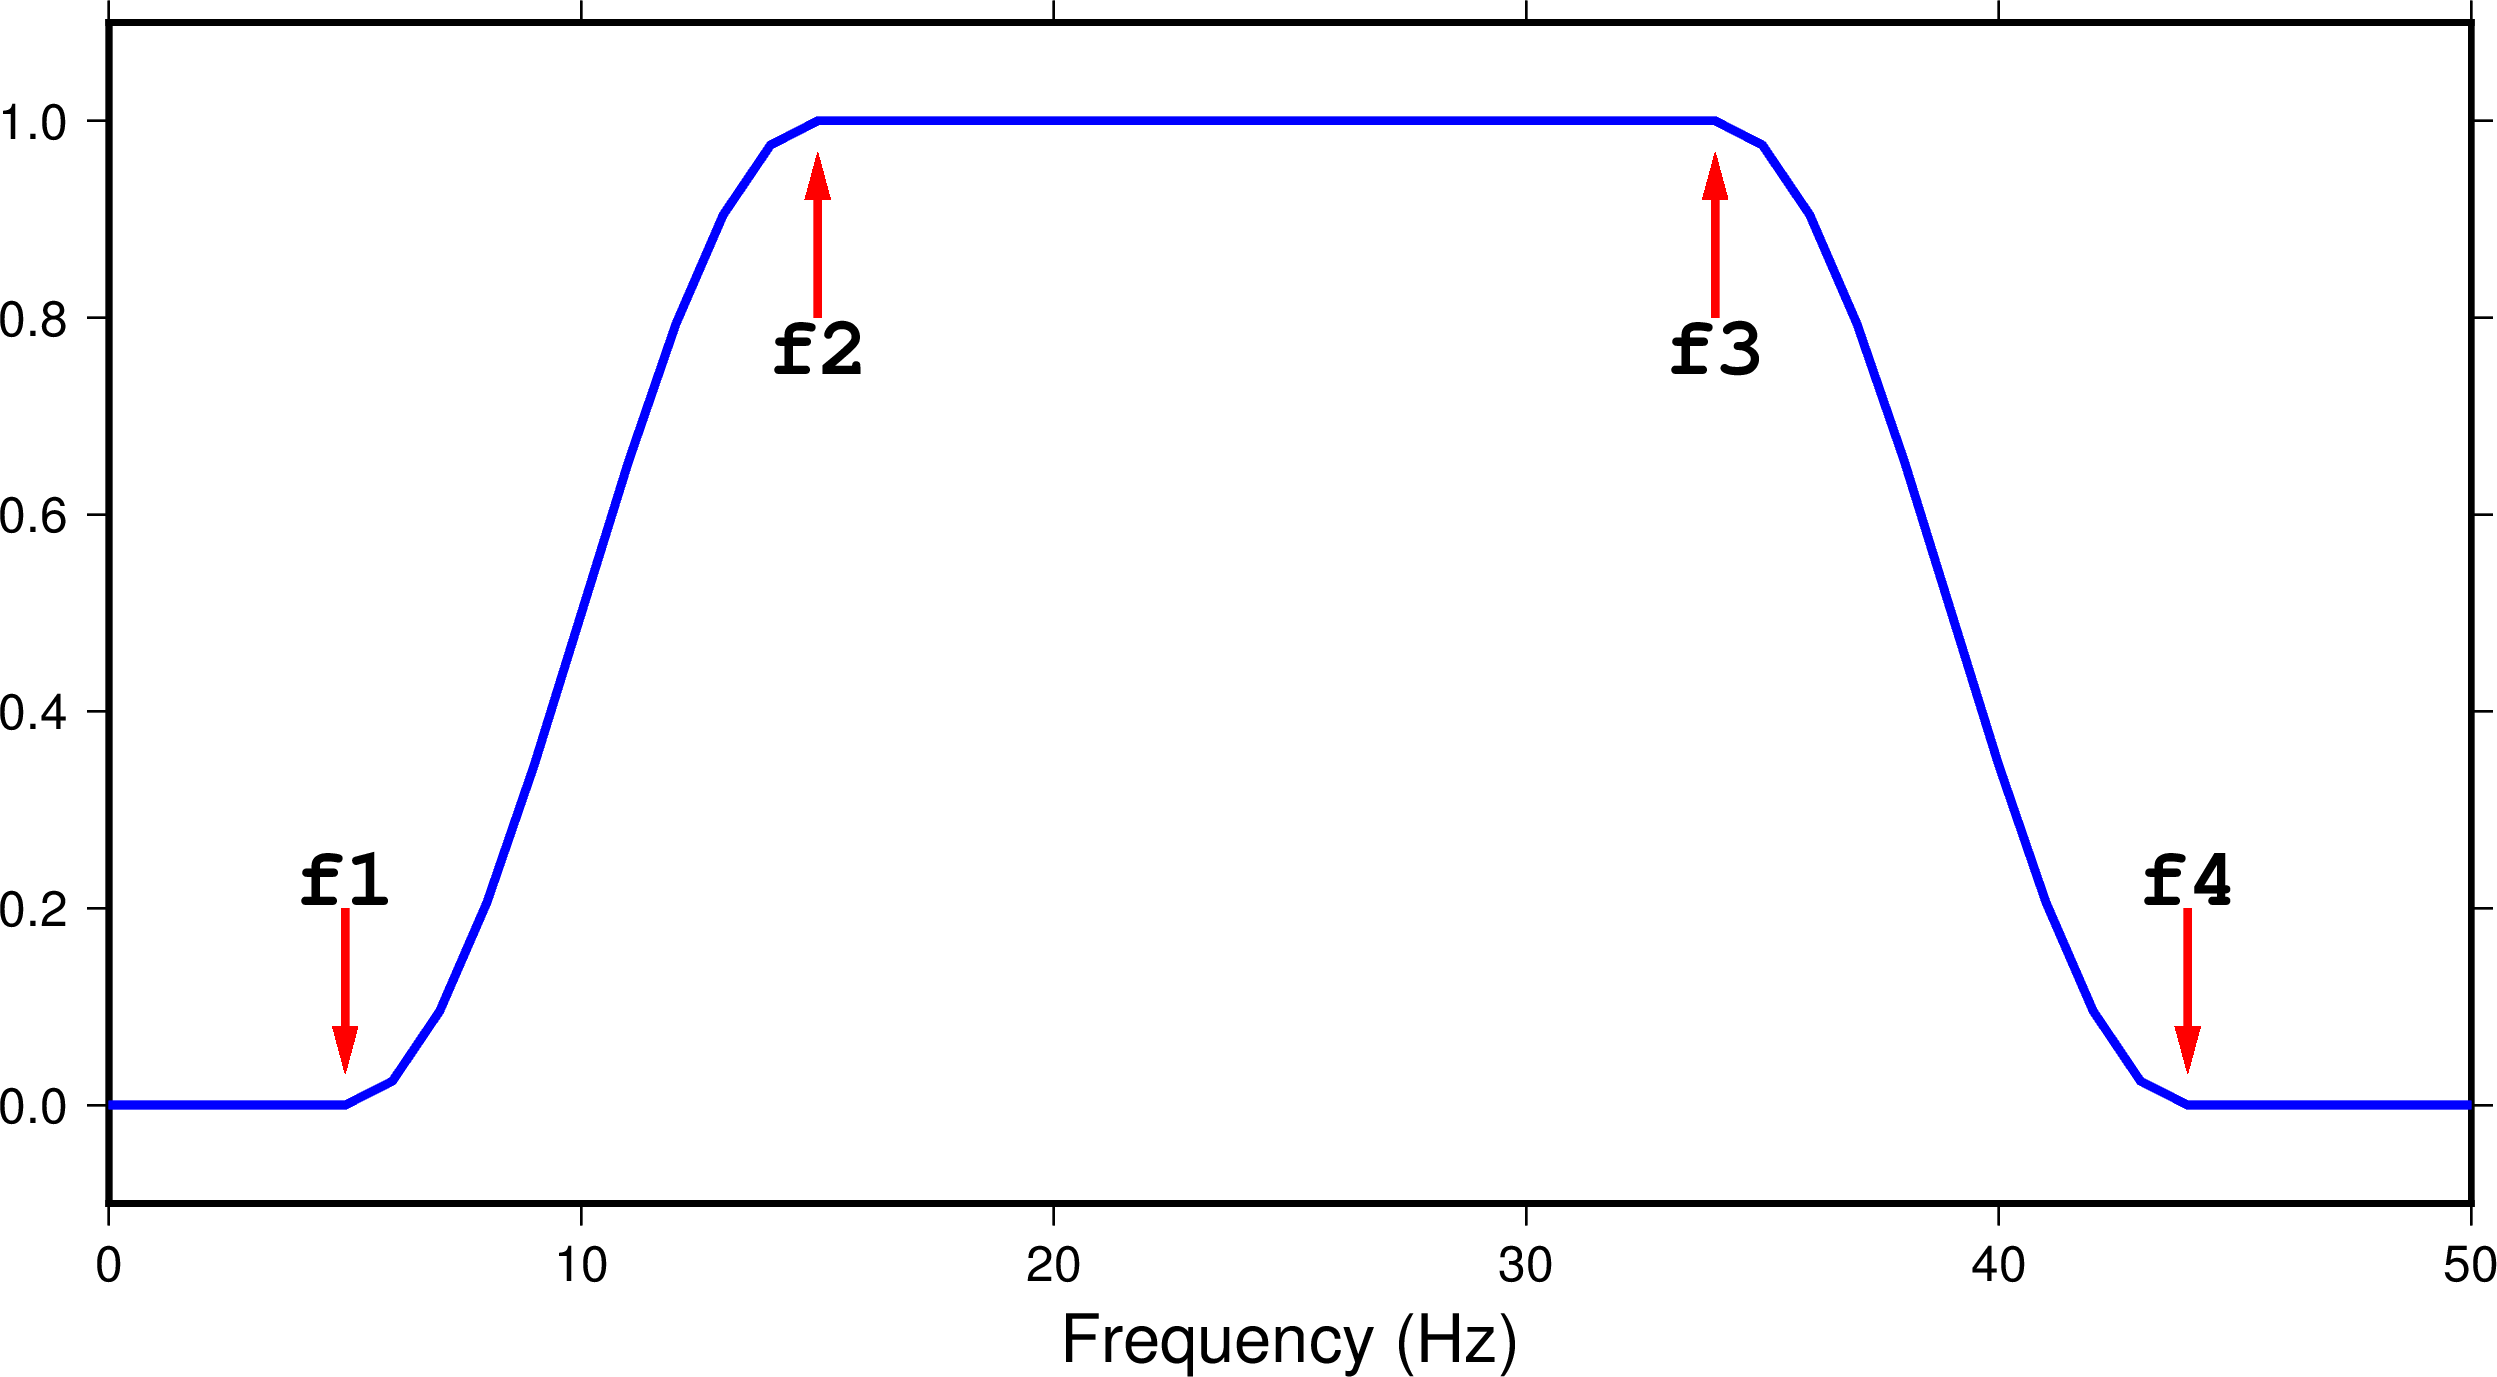
\includegraphics[width=0.9\textwidth]{freqlimits}
\caption{Freqlimits尖灭函数}
\label{fig:freqlimits}
\end{figure}

四个频率参数除了要满足 \texttt{f1<f2<f3<f4} 外,还应注意如下几条原则:
\begin{itemize}
\item \texttt{f4} 应小于Nyquist采样率。比如若数据的采样周期为 \SI{0.01}{\s},则Nyquist采样率
    为 \SI{50}{\Hz},因而f4应小于\SI{50}{\Hz};
\item f3不能与f4太接近;
\item f2与f3之间应尽可能宽,然后再根据具体需求进行滤波;
\item f1和f2不能太接近;
\item f1的选取由具体需求决定,可以尝试不同的值并查看去仪器响应之后的效果来决定;
\end{itemize}

若想要一个低通滤波器但在低频处不滤波,可以设置 \texttt{f1=-2} 和 \texttt{f2=-1};
若想要一个高通滤波器但在高频处不滤波,可以设置f3等于Nyquist频率,f4为Nyquist频率的两倍。

需要注意,该滤波器是零相位、非因果滤波器,因而,若数据点数不为2的指数幂次,
会导致在频段 \texttt{(f1,f4)} 之外振幅不完全为0。若想要数据点数为2的幂次方,
可以参考SAC中的 \nameref{cmd:cut} 命令。

\subsubsection{prewhitening}
\texttt{prewhitening} 用于控制数据的预白化。预白化可以将输入时间序列在变换到
频率域之前,进行谱的平化。这会减小谱值的动态范围,并提高数据在高频的计算精度。
参见 \nameref{cmd:whiten} 命令。打开预白化选项,会在谱操作之前在频率域进行谱白化,
并在谱操作后在时间域做谱白化的补偿,也可以设置预白化选项的阶数。默认情况下,
预白化选项是关闭的,阶数为 \texttt{n=6}。

\SACTitle{示例}
\subsubsection{内置仪器类型}
SAC中内置了一堆预定义的仪器类型,可以在命令中直接使用。

从数据中去除LLL宽频带仪器响应。并卷积上SRO仪器响应,且对频带做尖灭及预白化:
\begin{SACCode}
SAC> read abc.z
SAC> rmean; rtr; taper
SAC> trans from lll to sro freq .02 .05 1. 2. prew 2
\end{SACCode}

当前的仪器类型为RSTN的子类型nykm.z,为了去除该仪器响应并卷积上DSS仪器响应:
\begin{SACCode}
SAC> read nykm.z
SAC> rmean; rtr; taper
SAC> trans from rstn subtype nykm.z to dss prew off
\end{SACCode}

将电磁仪器响应转换成位移:
\begin{SACCode}
SAC> r XYZ.Z
SAC> trans from elmag freep 15. mag 750. to none
\end{SACCode}

从波形中去除WWSP的仪器响应,得到位移波形:
\begin{SACCode}
SAC> read xyz.z
SAC> rmean; rtr; taper
SAC> trans from WWSP to none freq 0.05 0.01 5 10
                // 也可使用to vel或to acc得到速度或加速度
\end{SACCode}

向合成的位移地震图中加入WWSP仪器响应:
\begin{SACCode}
SAC> r syn.z
SAC> trans from none to WWSP    // 简写为trans to WWSP
\end{SACCode}

\subsubsection{evalresp类型}
\texttt{evalresp} 类型并不代表真正意义上的仪器类型,而是表示从RESP仪器响应文件中
读取仪器响应信息。在使用 \texttt{evalresp} 选项时,\nameref{cmd:transfer} 依次从
当前内存中的SAC波形数据中提取出各自的头段信息,包括:\texttt{kstnm}、\texttt{kcmpnm}、
\texttt{kzdate}、\texttt{kztime}、\texttt{knetwk} 和 \texttt{locid},然后会在当前目录下
寻找文件名为``\texttt{RESP.<NET>.<STA>.<LOCID>.<CHN>}''的RESP文件(比如``RESP.IU.COLA..BHZ''),
并检测RESP文件中给出的台站信息是否与数据中的台站信息匹配
\footnote{即,要求RESP文件名以及RESP文件中的台站信息都与数据头段中的台站信息匹配}。
\begin{SACCode}
SAC> r 2006.253.14.30.24.0000.TA.N11A..LHZ.Q.SAC
SAC> rtr; rtr; taper
SAC> trans from evalresp to none freq 0.004 0.007 0.2 0.4
\end{SACCode}
该命令会首先从头段中提取台站信息,然后自动在当前目录下寻找文件 \texttt{RESP.TA.N11A..LHZ},
一旦文件中的台站信息与数据中的台站信息匹配,则使用该响应函数。

SAC数据中的头段信息可以用一些选项来覆盖:
\begin{verbatim}
    STATION, CHANNEL, NETWORK, DATE, TIME, LOCID, FNAME
\end{verbatim}
每个选项都必须有一个合适的值。若DATE在SAC头段中未设定且在选项中未指定,
则使用当前系统日期,TIME同理;若NETWORK未指定,则默认使用任意台网名;
若LOCID或KHOLE未指定,则默认使用任意LOCID。

假设台网IU的所有台站都具有完全相同的仪器响应函数,而此时你只有COLA台站的RESP
文件``RESP.IU.COLA..BHZ''。为了给所有台站去除仪器响应,一种办法是对IU台网的每一个
台站复制一份``RESP.IU.COLA..BHZ'',重命名,并修改RESP文件中的台站信息。显然,这样
很麻烦,利用上面的选项可以大大简化这一过程:
\begin{SACCode}
SAC> r *.IU.*.BHZ
SAC> rmean; rtr; taper
SAC> trans from evalresp STATION COLA to none freq 0.01 0.02 5 10
\end{SACCode}
使用STATION选项覆盖了波形数据中的台站名,此时,对每一个波形数据,transfer命令都会
去使用``RESP.IU.COLA..BHZ''\footnote{这里假定所有台站的LOCID都是未定义的}。

下面的命令会将三分量数据去仪器响应,并卷积上BHZ分量的仪器响应:
\begin{SACCode}
SAC> r *.IU.COLA.00.BH?
SAC> rmean; rtr; taper
SAC> trans from evalresp to evalresp CHANNEL BHZ
\end{SACCode}
操作完成后,BHZ分量相当于没有进行操作,BH1和BH2则去除了原本的仪器响应并卷积上BHZ的
仪器响应。

为了显示IU台网COL台站BHZ通道,1992年01月02日16:42:05的仪器响应:
\begin{SACCode}
SAC> fg impulse npts 16384 delta .05 begin 0.
SAC> trans to evalresp sta COL cha BHZ net IU \
                    date 1992/2 time 16:42:05
SAC> fft
SAC> psp am
\end{SACCode}

如果你的RESP文件名与SAC的标准格式不同,可以使用FNAME选项强制指定要使用的RESP文件:
\begin{SACCode}
SAC> r 2006.253.14.30.24.0000.TA.N11A..LHZ.Q.SAC
SAC> rmean; rtr; taper
SAC> trans from evalresp fname /tmp/Resp/RESP.TA.N11A..LHZ to none \
                        freq 0.004 0.007 0.2 0.4
\end{SACCode}
transfer命令默认会使用``RESP.TA.N11A..LHZ''作为响应文件,此处使用FNAME选项强制指定
使用``/tmp/RESP/RESP.TA.N11A..LHZ''。需要注意的是,即便是使用FNAME强制指定了RESP文件,
该命令还是会检测台站信息是否匹配。

由于一个RESP文件中可以包含多个响应函数,因而可以将所有仪器响应文件合并到一个总的
RESP文件中:
\begin{SACCode}
SAC> r *.SAC
SAC> rmean; rtr; taper
SAC> transfer from evalresp fname RESP.ALL to none freq 0.1 0.2 5 10
\end{SACCode}
这个例子中,RESP.ALL包含了所有数据的响应函数,transfer命令会读取RESP.ALL文件的内容,
对于每一个波形数据,会从波形数据中提取出台站信息,并与RESP.ALL中的众多响应函数进行
匹配,若匹配成功,则使用该响应函数。

\subsubsection{polezero类型}
\texttt{polezero} 类型并不代表真正意义上的仪器类型,而是表示从SAC零极点文件中读取仪器
响应函数。

polezero类型会从数据波形中提取台站信息,但不会根据台站信息去寻找默认的PZ文件,用户
必须使用 \texttt{subtype} 来指定要使用的PZ文件。若PZ文件有注释行,则注释行中的台站信息
必须与波形中的台站信息匹配,才能正确执行;若PZ文件中无注释行,则不进行台站信息匹配
的检测,直接执行。
\begin{SACCode}
SAC> r *IU.COLA.BHZ
SAC> rmean; rtr; taper
SAC> trans from polezero subtype SAC_PZs.IU.COLA.BHZ to WWSP
\end{SACCode}

一个PZ文件中可以包含多台站、多通道、多时间段的响应函数。可以将所有数据的PZ
文件合并得到总的PZ文件。下面的例子中读入全部波形数据,并利用总PZ文件进行去
仪器响应:
\begin{SACCode}
SAC> r *.SAC          // 读入全部数据
SAC> rmean; rtr; taper
SAC> trans from polezero s event.pz to none freq 0.05 0.1 10.0 15.0
SAC> mul 1.0e9        // 需要乘以1.0e9 !!!!!
SAC> w over
\end{SACCode}

需要格外注意,在用PZ文件去仪器响应得到位移物理量时,得到的数据的单位是 \texttt{m},
而SAC中默认的单位是 \texttt{nm},因而需要将数据乘以 \texttt{1.0e9} 将数据的单位
转换成 \texttt{nm}。对于转换得到速度或加速度,同理。

\subsubsection{fap选项}
fap选项表明使用FAP文件作为响应函数。

假设有fapfile文件 \verb|fap.n11a.lhz_0.006-0.2|,其名字表示频率段为
\SI{0.006}{\Hz} 到 \SI{0.2}{\Hz},
要从波形 \texttt{2006.253.14.30.24.0000.TA.N11A..LHZ.Q.SAC} 中移除该仪器响应:
\begin{SACCode}
SAC> r 2006.253.14.30.24.0000.TA.N11A..LHZ.Q.SAC
SAC> rtr
SAC> taper
SAC> trans from fap s fap.n11a.lhz_0.006-0.2 to none \
                        freq 0.004 0.006 0.1 0.2
SAC> mul 1.0e9
\end{SACCode}

\SACCMD{traveltime}
\label{cmd:traveltime}

\SACTitle{概要}
根据预定义的速度模型计算指定震相的走时

\SACTitle{语法}
\begin{SACSTX}
T!RAVEL!TIME [MODEL string] [PICKS number] [PHASE phase list]
    [VERBOSE|QUIET] [M|KM]
\end{SACSTX}

\SACTitle{输入}
\begin{description}
\item [MODEL] iasp91或ak135,缺省为iasp91
\item [PICKS] 如果number值位于0到9,则第一个震相的到时将储存在头段Tn中。如果命令行选项中没有包含PICKS,VERBOSE就会打开并显示震相到时而不写入头段。
\item [PHASE] 要pick或显示的震相列表,如果有PICKS n选项,则则震相到时以及其标签将写入到头段Tn和KTn中。
\item [VERBOSE|QUIET] 若使用VERBOSE,则震相走时将以相对发震时刻(O)和文件起始时间(B)两种方式显示;若使用QUIET,则不在屏幕上显示到时,若二者都没有显示,则显示traveltime命令使用的深度
\item [M|KM] 头段变量evdp的单位为 \si{\m} 或者 \si{\km}
\end{description}

\SACTitle{缺省值}
\begin{SACDFT}
traveltime MODEL iasp91 KM PHASE P S Pn Pg Sn Sg
\end{SACDFT}

\SACTitle{说明}
该命令使用iaspei-tau
\footnote{\url{https://seiscode.iris.washington.edu/projects/iaspei-tau}}
程序计算走时,要求内存中的波形文件的事件和台站位置以及发震时刻必须定义。

内存中所有文件拾取的震相的到时存储在头段变量Tn中,其中n的范围为0到9。计算的走时是相对于发震时刻(O)的,但存储在Tn中的时间是相对于文件起始时间(B)。

走时表根据地震深度及震中距获得走时,震中距(gcarc)使用球三角几何,根据事件和台站经纬度计算。

由于历史原因,事件深度evdp以前的单位为 \si{\m},rdseed产生的SAC波形数据单位为 \si{\m}。
在新版的SAC中,默认的evdp单位为 \si{\km},但由于很多波形数据evdp仍然为 \si{\m},这里引入这个
命令选项以指定深度单位。

在SAC2000中,命令traveltime位于子程序SSS中,当前版本(v101.5)没有SAC2000版本的全部功能,
但可以不用进入SSS而直接运行。

\SACTitle{示例}
区域事件,使用默认震相:
\begin{SACCode}
SAC> fg seismo
SAC> traveltime
traveltime: depth: 15.000000
traveltime: error finding phase P
traveltime: error finding phase S
traveltime: setting phase Pn       at 10.464321 s [ t = 51.894321 s ]
traveltime: setting phase Pg       at 22.904724 s [ t = 64.334724 s ]
traveltime: setting phase Sn       at 50.047722 s [ t = 91.477722 s ]
traveltime: setting phase Sg      at 66.414337 s [ t = 107.844337 s ]
\end{SACCode}

对于区域事件,初至波为Pn或Pg,因而这里没有P波到达,对上面的例子,拾取不会写入头段中。
\begin{SACCode}
SAC> fg seismo
SAC> traveltime picks 0 phase Pn Pg Sn Sg
traveltime: depth: 15.000000
SAC> lh AMARKER T0MARKER T1MARKER T2MARKER T3MARKER
AMARKER = 10.464
T0MARKER = 10.464           (Pn)
T1MARKER = 22.905           (Pg)
T2MARKER = 50.048           (Sn)
T3MARKER = 66.414           (Sg)
SAC> write seismo-picks.z
\end{SACCode}
可以看到已经将A定义为Pn的到时,文件seismo-picks.z将有T0到T3四个头段,
命令PLOT1可以看到有各震相在相应到时处有标签名。
注意尽管VERBOSE没有开启,深度(单位 \si{\km})还是会被打印出来。
这是为了保证用户对EVDP的单位有正确的了解,可以通过QUIET选项取消深度的显示。

下面例子给出的波形文件是由rdseed v5.0产生的,震源深度evdp的单位为 \si{\m}:
\begin{SACCode}
SAC> r 2008.052.14.16.03.0000.XC.OR075.00.LHZ.M.SAC
SAC> lh evdp
evdp = 6.700000e+03
SAC> traveltime M picks 0
traveltime: depth: 6.700000 km
SAC> lh t0marker t1marker t2marker t3marker
t0marker = 61.48            (Pn)
t1marker = 76.413           (Pg)
t2marker = 109.66           (Sn)
t3marker = 132.11           (Sg)
SAC> ch evdp (0.001 * :1,evdp:)
SAC> setbb station :1,KSTNM:
SAC> write %station%.z
\end{SACCode}
保存的文件OR075.z单位为 \si{\km},并且各个震相Pn、Pg、Sn及Sg都有注释。
震相名是大小敏感的,具体参见iaspei-tau的文档。

\SACCMD{tsize}
\label{cmd:tsize}

\SACTitle{概要}
控制文本尺寸属性

\SACTitle{语法}
\begin{SACSTX}
TSIZE [T!INY!|S!MALL!|M!EDIUM!|L!ARGE! v ] [RATIO v] [OLD|NEW]
\end{SACSTX}

\SACTitle{输入}
\begin{description}
\item [TINY|SMALL|MEDIUM|LARGE v] 设定标准文本尺寸的值为v
\item [RATIO v] 设定文本的宽高比为v
\item [OLD] 将所有文本尺寸值设置为旧值。旧值即SAC 9之前的版本中的文本尺寸值
\item [NEW] 设定所有文本尺寸值为SAC初始化时的缺省值
\end{description}

\SACTitle{缺省值}
\begin{SACDFT}
tsize ratio 1.0 new
\end{SACDFT}

\SACTitle{说明}
大多数的文本注释命令(\nameref{cmd:title}、\nameref{cmd:xlabel}、\nameref{cmd:fileid}等)
允许你改变要显示的文本的尺寸。
你可以从四个标准尺寸中选择(TINY、SMALL、MEDIUM、LARGE)。每一个标准尺寸都有一个初始值,
如下表所示,这个尺寸定义为一个字符的高度相对于整个视窗的百分比。有些时候你想要使用一些
不同于默认尺寸的文本。\nameref{cmd:tsize} 允许你重新定义这四个标准尺寸。你也可以使用这个命令改变字符的宽-高比。
\begin{table}[!ht]
\centering
\caption{SAC标准文本尺寸}
\begin{tabular}{lccccc}
\toprule
NAME	&	A	&	B	&	C	&	D	&	E	\\
\midrule
TINY 	& 0.015 &   66 	&  50  	&	68  &	110	\\
SMALL	& 0.020 &	50  &  37  	&	66  &	82	\\
MEDIUM  & 0.030 &	33  &  25  	&	44  &	55	\\
LARGE	& 0.040 &	25  &  18  	&	33  &	41	\\
\bottomrule
\end{tabular}
\end{table}

上面做各列的定义如下:
\begin{itemize}
\item A 自如相对整个视窗的高度
\item B 全视窗下文本的行数
\item C 正常视窗下文本的行数。正常视窗是指x为0.到1.,y为0.到0.75
\item D 正常视窗中,每行的最小字符数
\item E 正常视窗中每行字符的平均数
\end{itemize}

从SAC 9开始,系统的默认文本尺寸发生了变化,新的尺寸集覆盖了更宽的尺寸范围,在
多数设备上看上去更好。你可以使用OLD选项将文本尺寸修改为之前版本的文本尺寸。

\SACTitle{示例}
为了改变MEDIUM的定义,并使用它创建一个特别尺寸的标题:
\begin{SACCode}
SAC> tsize medium 0.35
SAC> title 'rayleigh wave spectra' size medium
SAC> plot2
\end{SACCode}

为了重置文本尺寸到其默认值:
\begin{SACCode}
SAC> tsize new
\end{SACCode}

\SACCMD{unsetbb}
\label{cmd:unsetbb}

\SACTitle{概要}
删除黑板变量

\SACTitle{语法}
\begin{SACSTX}
UNSETBB ALL|variable ...
\end{SACSTX}

\SACTitle{输入}
\begin{description}
\item [ALL] 删除当前定义的全部黑板变量
\item [variable] 删除黑板变量variable
\end{description}

\SACTitle{说明}
参见\nameref{cmd:setbb}命令的说明

\SACTitle{示例}
一次删除多个黑板变量:
\begin{SACCode}
SAC> unsetbb c1 c2 x
\end{SACCode}

删除所有黑板变量:
\begin{SACCode}
SAC> unsetbb all
\end{SACCode}

\input{commands/unwrap}
\SACCMD{vspace}
\label{cmd:vspace}

\SACTitle{概要}
改变图形的最大尺寸和形状

\SACTitle{语法}
\begin{SACSTX}
VSP!ACE! FULL|v
\end{SACSTX}

\SACTitle{输入}
\begin{description}
\item [FULL] 使用整个视窗,这是可能的最大屏幕或窗口尺寸
\item [v] 使视窗比y:x为v,具有这个纵横比的最大的区域称为视窗
\end{description}

\SACTitle{缺省值}
\begin{SACDFT}
vspace full
\end{SACDFT}

\SACTitle{说明}
视窗代表了屏幕上可以用于绘图的部分。视窗形状和尺寸在不同图形设备之间有很大的变化。
\begin{enumerate}
\item 尽管在尺寸上有很大不同,许多图形终端都具有0.75的纵横比。
\item SGF文件的纵横比为0.75,其大约是标准的8.5*11英寸纸张的纵横比。
\item  由XWINDOWS或SUNWINDOWS图形设备建立的窗口可以有你想要的任意纵横比
\end{enumerate}

这个命令可以控制纵横比,从而使你能够控制图形的形状缺省绘图是在整个视窗上。
如果确定了一个纵横比,则视窗就是设备上具有这个纵横比的最大区域。

当你使用 \nameref{cmd:plotc} 命令在交互设备上建立一张图,并且最终要将它发送到SGF设备上,
这个命令特别有用,在绘制任何图形之前,必须设置纵横比为0.75。这将保证图形在SGF
文件上与在交互设备上相同。如果你要建立一个独立于图形设备的正方形视窗,
则可以简单地设置纵横比为1.0。

\SACCMD{wait}
\label{cmd:wait}

\SACTitle{概要}
控制SAC在输出大量文本或绘制多个图形时是否暂停

\SACTitle{语法}
\begin{SACSTX}
WAIT [T!EXT! ON|OFF] [P!LOTS! ON|OFF|E!VERY!]
\end{SACSTX}

\SACTitle{输入}
\begin{description}
\item [TEXT ON|OFF] 打开/关闭文本等待选项
\item [PLOTS ON|OFF] 打开/关闭绘图等待选项
\item [PLOTS EVERY] 每个图形之间均等待
\end{description}

\SACTitle{缺省值}
\begin{SACDFT}
wait text on plots on
\end{SACDFT}

\SACTitle{说明}
\texttt{TEXT} 选项用于控制当SAC输出到终端的内容超过一屏时,是等待用户
输入,还是继续输出。

\texttt{PLOTS} 选项用于控制绘制多张图时是否要暂停。在读取多个数据文件
并 \texttt{plot} 命令绘图时,每个文件将产生一个frame,正常情况下SAC将
在每张图后暂停并发送信息``Waiting''到终端,用户键入回车即可看到下一张图,
或输入``Go''使SAC不暂停地绘制剩下的图形,或键入``Kill''终止绘制这组文件。
SAC绘制完最后一张图后不再暂停,因为SAC的输入提示符已经实现了暂停功能。
当这个选项关闭时,SAC在不同的绘图间不暂停。

\SACCMD{whiten}
\label{cmd:whiten}

\SACTitle{概要}
平滑输入的时间序列的频谱

\SACTitle{语法}
\begin{SACSTX}
W!H!IT!EN! n [F!ILTER!D!ESIGN!]
\end{SACSTX}

\SACTitle{输入}
\begin{description}
\item [n]  阶数(极数)。这个数越大,结果数据就越平滑。高阶可以更好的清除一些数据,但是也可能会导致对数据处理过多而丢掉一些重要的数据。默认值为6。
\item [FD] 进行一些类似于filterdesign的命令,使用白化系数,设计一个白化滤波器。详情可以参考filterdesign命令。
\end{description}

\SACTitle{缺省值}
\begin{SACDFT}
whiten 6
\end{SACDFT}

\SACTitle{说明}
对数据中加入白噪声。平滑输入时间序列的频谱。当这个命令在谱分析命令(比如子程序SPE中的命令、transfer或spectrogram)之前执行,其减少了频谱值的动态范围,提供了对地震数据高频操作的精度。

WHITEN可以在SPE子程序内部调用,或者从SAC主程序中调用。SPE中的WHITEN和主程序中的
WHITEN分别有不同的阶数。在主程序中,你可以调用WHITEN 4,下一次在主程序中调用
WHITEN时阶数为4,但是在SPE中调用WHITEN时依然是缺省的6阶,除非你在SPE的命令行中
进行了修改。进一步,SPE中的阶数与SPE COR命令的PREWHITEN选项是一样的
(设置了一个其他的也就设置了)。当然主程序中WHITEN命令与TRANSFER命令中的
PREWHITEN选项也是一样的。

\SACCMD{whpf}
\label{cmd:whpf}

\SACTitle{概要}
将辅助内容写入HYPO格式的震相拾取文件中

\SACTitle{语法}
\begin{SACSTX}
WHPF IC n m
\end{SACSTX}

\SACTitle{输入}
\begin{description}
\item [IC n m]  在第18和19列插入带有两个整数的n和m的指令卡。n的允许值为0、1、5,m的允许值为0、1、9。
\end{description}

\SACTitle{说明}
``指令卡''用于分开在HYPO文件中的不同事件,参见HYPO71手册。关闭一个已经打开的HYPO震相拾取文件(CHPF)或者退出SAC时,将自动添加``10''指令卡到震相读取文件中。

\SACCMD{width}
\label{cmd:width}

\SACTitle{概要}
控制线宽

\SACTitle{语法}
\begin{SACSTX}
WIDTH [ON|OFF|width] [SK!ELETON! width] [I!NCREMENT! ON|OFF]
    [L!IST! S!TANDARD!|widthlist]
\end{SACSTX}
其中 \texttt{width} 只能取整数

\SACTitle{输入}
\begin{description}
\item [WIDTH width] 设置数据的线宽为 \texttt{width}
\item [WIDTH ON] 打开 \texttt{WIDTH} 选项但是不改变当前线宽值
\item [WIDTH OFF] 关闭 \texttt{WIDTH} 选项
\item [SKELETON width] 设置图形边框宽度为 \tetxtt{width}
\item [LIST STANDARD] 设置为标准线宽列表,设置数据宽度为标准列表中的
    第一个宽度,并打开 \texttt{WIDTH} 选项
\item [LIST widthlist] 改变宽度列表的内容。输入宽度列表。设置数据宽度
    为列表中的第一个宽度,并打开 \texttt{WIDTH} 选项
\item [INCREMENT ON] 按照 \texttt{widthlist} 表中的次序,依次改变一个宽度值
\item [INCREMENT OFF] 关闭线宽递增功能
\end{description}

\SACTitle{缺省值}
\begin{SACDFT}
width off skeleton 1 increment off list standard
\end{SACDFT}

\SACTitle{说明}
\texttt{width} 指定了绘制数据时的线条宽度。\texttt{SKELETON}指定了
坐标轴的宽度,其就仅修改坐标轴的宽度,网格、文本、标签和框架号总是
用1号细线表示。

若将WIDTH设置为递增,则每次绘图之后,宽度都会按照宽度表中的顺序自动修改。

如果在同一张绘图中同时绘制几个数据文件,也许需要对每个文件使用不同的宽度。
此时可使用INCREMENT选项。在这个选项打开时,每次绘制一个数据文件后,都按照宽度表中的
次序自动地变成另一个宽度。宽度值和次序在标准宽度表中为:
\begin{SACCode}
1, 2, 3, 4, 5, 6, 7, 8, 9, 10
\end{SACCode}
你可以使用LIST选项改变这个表的次序或内容。这个命令常用于重叠绘图(参见PLOT2),
此时你可能需要每张图上的数据宽度都按相同的顺序排列。

\SACTitle{示例}
选择自动变换的数据宽度起始值为1:
\begin{SACCode}
SAC> width 1 increment
\end{SACCode}

边框宽度起始值为2,并按1、3、5的增量变化:
\begin{SACCode}
SAC> width skeleton 2 increment list 1 3 5
\end{SACCode}

\SACCMD{wiener}
\label{cmd:wiener}

\SACTitle{概要}
设计并应用一个自适应Wiener滤波器

\SACTitle{语法}
\begin{SACSTX}
W!IE!N!E!R [W!INDOW! pdw] [N!COEFF! n] [MU OFF|ON|v] [EPS!ILON! OFF|ON|e]
\end{SACSTX}

\SACTitle{输入}
\begin{description}
\item [WINDOW pdw] 设置滤波器设计窗口为pdw。关于pdw参见 \nameref{cmd:cut} 命令
\item [NCOEFF n] 设置滤波器系数为n个
\item [MU off|on|v] 设置自适应步长参数
\item [MU Off] 设置自适应步长参数为0
\item [MU ON] 设置自适应步长为1.95/Rho(0),其中Rho(0)是pdw中延迟为0时的自相关系数
\item [MU v] 设置自适应步长为v
\item [EPSILON e] 设置ridge回归参数为e。
\end{description}

\SACTitle{缺省值}
\begin{SACDFT}
wiener window b 0 10 ncoeff 30 mu off epsilon off
\end{SACDFT}

\SACTitle{说明}
预测误差滤波器使用Yule-Walker方法,从指定的部分数据窗中由自相关函数给出。
这个窗口可以是文件的任何部分,然后滤波器应用到整个个信号,即信号被残差序列替换。
这个滤波器可以用作预白化或用作瞬时信号的检波预处理器。若mu指定为非0值,则滤波器
为时域自适应的,大值mu可能会导致不稳定。

\SACTitle{示例}
下面的命令将应用一个非自适应滤波器,将第一个十秒指定为窗:
\begin{SACCode}
SAC> wiener window b 0 10 mu 0.
\end{SACCode}

下面命令将应用带40个系数的滤波器,指定设计窗为从文件开始到第一个到时前1秒:
\begin{SACCode}
SAC> wiener ncoeff 40 window b a -1
\end{SACCode}

\SACTitle{头段变量}
depmin、depmax、depmen

\SACTitle{相关命令}
\nameref{cmd:cut}

\SACCMD{wild}
\label{cmd:wild}

\SACTitle{概要}
设置读命令中用于扩展文件列表的通配符

\SACTitle{语法}
\begin{SACSTX}
WILD [ECHO ON|OFF] [SINGLE char] [MULTIPLE char] [CONCATENATION chars]
\end{SACSTX}

\SACTitle{输入}
\begin{description}
\item [ECHO ON] 打开扩展文件表回显选项;当该选项打开时,会回显被通配符展开的文件列表
\item [ECHO OFF] 关闭扩展文件表回显开关
\item [SINGLE char] 修改用于匹配单个字符的通配符
\item [MULTIPLE char] 修改用于匹配多个字符的通配符
\item [CONCATENATION chars] 修改用于将联接字符串括起来的字符
\end{description}

\SACTitle{缺省值}
\begin{center}
\begin{tabular}{llll}
\toprule
选项	&	UNIX	&	VAX		&	PRIME	\\
\midrule
ECHO	&	ON 		&	ON 		&	ON		\\
SINGLE  &	?  		&	?  		&	+		\\
MULTIPLE&	* 		&	* 		&	'		\\
CONCATENATION& [,] & 	(,)  	&	[,]		\\
\bottomrule
\end{tabular}
\end{center}

\SACTitle{说明}
很多现代操作系统都提供了通配符特性,也可以称为文件扩展。它是一个可以让你使用
简短文件名以及简单的简写形式去指定一组文件的表示符号。SAC在READ、READTABLE以及READHDR
命令中使用通配符及一些扩展名,使用这些表示符号,你可以很容易地访问一组文件:
\begin{itemize}
\item 所有以字母``abc''开头的文件
\item 所有以``z''结尾的文件
\item 所有文件名中严格包含三个字母的文件
\end{itemize}

通配符代号有三个元素。对于不同的系统三个元素会有不同的缺省符。你可以使用这个命令改变通配符。多重匹配字符(``*'')用于匹配字符串中任意字符串,包括空字符串。单个匹配符(``?'')用于匹配任意单个字符。连接符号(``[''和``]'')用于包围由逗号分隔的要匹配的字符串。在这个字符串中,可以包含单通配符或多通配符。

SAC使用通配符完成文件名的扩展,通常有几个步骤:
\begin{enumerate}
\item 如果标识目录部分存在的话将将其去掉,否则使用当前目录
\item 做系统调用,以得到目录中所有文件的列表
\item 如果在标识中是一个连接表,就用其他字符形成连接表中每个字符的新的标识,然	  后匹配它们到文件表中。如果没有连接表标识,则可简单匹配标识到文件表
\item 去掉形成扩展文件表的所有重复的匹配
\item 如果需要,回显扩展文件表
\item 试着将扩展文件表读入内存
\end{enumerate}

每个操作系统都使用一些不同的步骤在一个目录中存取文件。上面第一步的系统调用反映了这些不同。例如,在UNIX中以字母顺序显示文件名,但在PRIME或VAX上就不是这样。在PRIME目录中文件次序是随意的。这些不同反映在扩展文件表的文件次序上。你可以用各种不同的通配符和连接表进行实验,以确定扩展文件表中的文件次序是否重要。

下例将帮助你理解怎样使用这些通配符元素,一个有用的特征是SAC保存包含在连接表上的字符串,当你输入一个空表,则前面的表将被重复使用,这可以节省许多输入的操作。

\SACTitle{示例}
假定当前目录中包含如下次序的文件:
\begin{SACCode}
ABC DEF STA01E STA01N STA01Z STA02E STA02N STA02Z STA03Z
\end{SACCode}

同样假定扩展文件设置回显,下面显示怎样使用各种通配符去将上面文件表的一部分读入内存:
\begin{SACCode}
SAC> READ S*
 STA01E STA01N STA01Z STA02E STA02N STA02Z STA03Z
SAC> READ *Z
 STA01Z STA02Z STA03Z
SAC> READ ???
 ABC DEF
SAC> READ STA01[Z,N,E]
 STA01Z STA01N STA01E
SAC> READ *[Z,N,E]
 STA01Z STA02Z STA03Z STA01N STA02N STA01E STA02E
SAC> READ *1[Z,N,E] *2[ ]
 STA01Z STA01N STA01E STA02Z STA02N STA02E
\end{SACCode}

\SACTitle{限制}
在一个标识中只可以有一个连接串

\input{commands/window}
\SACCMD{write}
\label{cmd:write}

\SACTitle{概要}
将内存中的数据写入磁盘

\SACTitle{语法}
\begin{SACSTX}
W!RITE! [SAC|ALPHA|XDR] [DIR OFF|CURRENT|name] [KSTCMP]
    [OVER|APPEND text|PREPEND text|DELETE text|CHANGE text1 text2]
    filelist
\end{SACSTX}

\SACTitle{输入}
\begin{description}
\item [无参数] 使用以前的数据格式和文件列表
\item [SAC] 以SAC二进制文件格式写入磁盘
\item [ALPHA] 写SAC字符数字型写入磁盘
\item [XDR] 用SAC二进制xdr格式写文件。这个格式用于实现不同构架的二进制数据的转换
\item [DIR OFF] 关闭目录选项,即写入当前目录
\item [DIR CURRENT] 打开目录选项并设置写目录为当前目录
\item [DIR name] 打开目录选项并设置写目录为name。将所有的文件写入目录name中,其可以是相对路径或绝对路径
\item [KSTCMP] 使用KSTNM和KCMPNM头段变量为内存中每个数据文件定义一个文件名。生成的文件名将检查是否唯一,如果不唯一,则在文件名后加序号以避免文件名冲突
\item [OVER] 使用当前读文件列表作为写文件列表,用内存中的文件覆盖磁盘中的文件
\item [APPEND text] 在当前读文件列表的文件名后附加字符串text以创建写文件列表
\item [PREPEND text] 在当前读文件列表的文件名前附加字符串text以创建写文件列表
\item [DELETE text] 在当前读文件列表的文件名中删除第一次出现的text以创建写文件表
\item [CHANGE text1 text2] 将当前读文件表中每个文件名中第一次出现的text1修改为text2来创建写文件表
\item [filelist] 将写文件列表设置为filelist,这个列表可以包含文件名、相对/绝对路径,不可以包含通配符。
\end{description}

\SACTitle{缺省值}
\begin{SACDFT}
write sac
\end{SACDFT}

\SACTitle{说明}
该命令允许你在数据处理的过程中将结果写入磁盘。写磁盘文件时可以选择几种数据格式,
内存中的每个文件都将完整地写入到磁盘中。

多数情况下,你会选择使用SAC数据文件格式,这是SAC软件的标准输入输出格式,用于快速读写,
其包含了以一个头段区和一个数据区。具体可以参考``\nameref{chap:sac-file-format}''一章。

你可以直接指定写文件名,也可以通过修改内存中的当前文件名间接地指定它们。
OVER选项把写文件表设置为读文件表。它用于覆盖包含当前内存的数据的读入的最后一组磁盘文件。
APPEND、PREPEND、DELETE、CHANGE选项通过以所需要的方式修改每个读文件名的方式建立一个
写文件表,这在宏命令中非常有用,在宏命令中你通常需要自动处理大量数据文件,并保持输出文件
风格的一致。当使用这四个选项中的任意一个时,命令执行时会在终端输出文件列表,使得你可以
看到实际写入磁盘的文件名。

\SACTitle{示例}
该命令的简单示例可以参考``\nameref{sec:read-and-write}''一节。

对一组数据文件进行滤波,然后将结果存入一组新数据文件:
\begin{SACCode}
SAC> read d1 d2 d3
SAC> lowpass butter npoles 4
SAC> write f1 f2 f3
\end{SACCode}

也可以使用CHANGE选项完成这一操作:
\begin{SACCode}
SAC> read d1 d2 d3
SAC> lowpass butter npoles 4
SAC> write change d f
\end{SACCode}

若想要用滤波后的数据替换磁盘中的原始数据,则上例的第三行要变成:
\begin{SACCode}
SAC> write over
\end{SACCode}

\SACCMD{writebbf}
\label{cmd:writebbf}

\SACTitle{概要}
将黑板变量文件写入到磁盘

\SACTitle{语法}
\begin{SACSTX}
W!RITE!BBF [file]
\end{SACSTX}

\SACTitle{输入}
\begin{description}
\item [file] 黑板变量文件的文件名
\end{description}

\SACTitle{缺省值}
\begin{SACDFT}
writebbf bbf
\end{SACDFT}

\SACTitle{说明}
该命令让你能够将当前会话的所有黑板变量写入到磁盘文件中,稍后可以使用
\nameref{cmd:readbbf} 命令将黑板变量文件重新读入SAC,该特性允许你保存
某次SAC会话的信息,并用于另一次SAC会话中。你也可以在自己的程序中调用
SAC函数库以访问黑板变量文件中的信息。

\SACCMD{writehdr}
\label{cmd:writehdr}

\SACTitle{概要}
用内存中文件的头段区覆盖磁盘文字中的头段区

\SACTitle{语法}
\begin{SACSTX}
W!RITE!H!DR!
\end{SACSTX}

\SACTitle{说明}
write命令的over选项可以用内存中头段区和数据区覆盖磁盘文件中的头段区和数据区。
该命令用内存中头段区覆盖磁盘文件中的头段区,数据区不会被覆盖。如果使用了cut命令,
读取数据时将仅读入部分数据,内存中的头段区将会做相应修改以反映cut命令的效果,
但是磁盘中的数据并没有被修改,因而此时不能使用writehdr命令。对被cut的数据
使用WRITEHDR命令将可能导致磁盘中的数据产生类似于平移或截断的效果。

\SACCMD{writesp}
\label{cmd:writesp}

\SACTitle{概要}
将谱文件作为一般文件写入磁盘

\SACTitle{语法}
\begin{SACSTX}
W!RITE!SP [ASIS|RLIM|AMPH|RL|IM|AM|PH] [OVER|filelist]
\end{SACSTX}

\SACTitle{输入}
\begin{description}
\item [ASIS]  按照谱文件当前格式写入
\item [RLIM]  写入实部和虚部分量
\item [AMPH]  写入振幅和相位分量
\item [RL]  只写入实部分量
\item [IM]  只写入虚部分量
\item [AM]  只写入振幅分量
\item [PH]  只写入相位分量
\item [filelist]  SAC二进制数据文件列表,这个列表可以包含简单文件名和绝对/相对路径名
\end{description}

\SACTitle{缺省值}
\begin{SACDFT}
writesp asis
\end{SACDFT}

\SACTitle{说明}
SAC数据文件可以为时间序列文件或谱文件。头段中的IFTYPE用于区分这两种格式。当你读取一个时间序列到内存,对其做快速Fourier变换,然后将数据写回磁盘,此时的文件即为谱文件。

某些操作只能对时间序列文件进行,而某些操作只能对谱文件进行。比如,你无法对一个谱文件应用taper命令或者将两个谱文件乘起来。这是SAC的保护机制。

然而有时你需要对谱文件做这些操作,为了越过SAC的保护机制,你可以使用这个命令将谱文件像时间序列数据一样写入磁盘。每一个分量都将作为一个单独文件写入磁盘。然后你可以将这些文件读入SAC并进行任何你想要的操作。因为SAC认为其为时间序列文件。一旦这些计算完成了,你可以将修改之后的数据通过WRITE命令写回磁盘。如果你想要读回这个谱文件,可以使用READSP命令。

为了帮助你跟踪磁盘上的数据,SAC将在你给出的文件名后加一个后缀以标识储存在文件的谱分量。后缀分别为``.RL'', ``.IM'', ``.AM''和``.PH''分别对应不同的分量。

\SACTitle{示例}
假设你想要对FILE1的谱文件振幅进行一些操作:
\begin{SACCode}
SAC> read file1
SAC> fft amph
SAC> writesp over
\end{SACCode}

SAC将输出两个文件FILE1.AM和FILE1.PH,现在可以对振幅文件进行操作:
\begin{SACCode}
SAC> read file1.am
SAC> ...perform operations.
SAC> write over
\end{SACCode}

现在磁盘中的文件为修改后的谱文件,如果你想要重建SAC谱数据并进行反变换:
\begin{SACCode}
SAC> readsp file1
SAC> ifft
SAC> write file2
\end{SACCode}

\SACTitle{头段变量改变}
磁盘文件中的b、e、delta将包含频率的起始值、结束值和增值,单位为 \si{Hz}

\SACCMD{xdiv}
\label{cmd:xdiv}

\SACTitle{概要}
控制x轴的刻度间隔

\SACTitle{语法}
\begin{SACSTX}
XDIV [NI!CE!|I!NCREMENT! v|NU!MBER! n] [P!OWER! ON|OFF]
\end{SACSTX}

\SACTitle{输入}
\begin{description}
\item [NICE] 由SAC自动选择合适的刻度间隔
\item [INCREMENT v] 设置刻度间隔增量为v
\item [NUMBER n] 设置刻度的总数目数为n
\item [POWER ON] 打开幂指数选项,SAC以幂指数形式给出刻度值
\item [POWER OFF] 关闭幂选项
\end{description}

\SACTitle{缺省值}
\begin{SACDFT}
xdiv nice power on
\end{SACDFT}

\SACTitle{说明}
该命令控制X轴的刻度间隔。多数时候默认的 \texttt{nice} 间隔即可满足需求。
SAC的 \texttt{nice} 刻度间隔是根据坐标轴的最小最大值、坐标轴的长度以及
当前坐标轴文本尺寸来决定的。

也可以使用 \texttt{INCREMENT} 选项强制刻度间隔为一个定值,或者使用
\texttt{NUMBER} 选项设置刻度间隔的数目。

\SACCMD{xfudge}
\label{cmd:xfudge}

\SACTitle{概要}
改变X轴的``插入因子''

\SACTitle{语法}
\begin{SACSTX}
XFUDGE [ON|OFF|v]
\end{SACSTX}

\SACTitle{输入}
\begin{description}
\item [ON] 打开插入选项,但不改变插入因子
\item [OFF] 关闭插入选项
\item [v] 打开插入因子,改变插入因子为v
\end{description}

\SACTitle{缺省值}
\begin{SACDFT}
xfudge 0.03
\end{SACDFT}

\SACTitle{说明}
当打开此选项时,实际轴范围将根据插入因子改变,确定线性坐标轴范围的方法是:
\[ XDIFF=XFUDGE*(XMAX-XMIN) \]
\[ XMIN=XMIN-XDIFF \]
\[ XMAX=XMAX+XDIFF \]
其中XMIN和XMAX是数据的极值,XFUDGE是插入因子,这个算法对于对数坐标也是相似的。
该选项仅当坐标轴的范围设置为数据极值时方可使用。

\SACCMD{xfull}
\label{cmd:xfull}

\SACTitle{概要}
控制X轴的绘图为整对数方式

\SACTitle{语法}
\begin{SACSTX}
XFULL [ON|OFF]
\end{SACSTX}

\SACTitle{输入}
\begin{description}
\item [ON|OFF] 打开/关闭整对数绘图选项
\end{description}

\SACTitle{缺省值}
\begin{SACDFT}
xfull on
\end{SACDFT}

\SACTitle{说明}
整对数绘图选项仅应用于使用对数坐标且坐标范围不固定(xlim off)的情况。当此选项打开时,
实际的坐标轴范围将被设置为数据范围前后的第一个整十数。当关闭这个选项时,将使用实际数据范围。

\SACCMD{xgrid}
\label{cmd:xgrid}

\SACTitle{概要}
控制绘图时的x方向的网格线

\SACTitle{语法}
\begin{SACSTX}
XGRID ON|OFF|S!OLID!|D!OTTED!
\end{SACSTX}

\SACTitle{输入}
\begin{description}
\item [SOLID] 设置网格线为实线
\item [DOTTED] 设置网格线为虚线
\item [ON] 绘制网格,但不改变网格类型
\item [OFF] 不绘制网格
\end{description}

\SACTitle{缺省值}
\begin{SACDFT}
xgrid off
\end{SACDFT}

\SACTitle{说明}
这个命令控制X坐标轴网格的绘制。

\SACCMD{xlabel}
\label{cmd:xlabel}

\SACTitle{概要}
定义X轴标签及属性

\SACTitle{语法}
\begin{SACSTX}
XLAB!E!L [ON|OFF|text] [L!OCATION! T!OP!|B!OTTOM!|R!IGHT!|L!EFT!]
    [S!IZE! T!INY!|S!MALL!|M!EDIUM!|L!ARGE!]
\end{SACSTX}

\SACTitle{输入}
\begin{description}
\item [text] 打开X轴标签选项,设置标签为 \texttt{text}。若文本含空格,
    需要用引号括起来
\item [ON] 打开X轴标签选项,但不改变标签文本
\item [OFF] 关闭X轴标签选项
\item [LOCATION] 设定X轴标签的位置。可以取 \texttt{TOP}、\texttt{BOTTOM}、
    \texttt{RIGHT}、\texttt{LEFT}
\item [SIZE] 改变绘图标签的文本尺寸
\item [TINY] 每行132个字符
\item [SMALL] 每行100个字符
\item [MEDIUM] 每行80字符
\item [LARGE] 大尺寸,每行50字符
\end{description}

\SACTitle{缺省值}
\begin{SACDFT}
xlabel off location bottom size small
\end{SACDFT}

\SACTitle{说明}
若打开X轴标签选项,则绘图时会在图上显示X轴标签。标签的尺寸和位置以及
文本均可以改变。文本质量以及字体可以使用 \nameref{cmd:gtext} 命令设置。

\SACCMD{xlim}
\label{cmd:xlim}

\SACTitle{概要}
设定图形中x轴的范围

\SACTitle{语法}
\begin{SACSTX}
XLIM [ON|OFF|pdw|SIGNAL]
\end{SACSTX}

\SACTitle{输入}
\begin{description}
\item [ON] 打开x轴范围选项,但不改变范围值
\item [OFF] 关闭x轴范围选项,即根据数据的自变量范围决定X轴范围
\item [pdw] 打开x轴范围选项并设置范围为新的``partial data window'',参考 \nameref{subsec:pdw}。
\item [SIGNAL] 等同于输入:``A -1 F +1'',即初至前1秒到事件结束的后1秒。
\end{description}

\SACTitle{缺省值}
\begin{SACDFT}
xlim off
\end{SACDFT}

\SACTitle{说明}
当此选项关闭时,根据数据自变量的范围决定绘图时x轴的范围。当此选项打开时,限定x轴的范围,
可以通过此种方式``放大''当前内存中数据的图形。

\SACTitle{相关命令}
\nameref{cmd:cut}

\input{commands/xlin}
\input{commands/xlog}
\SACCMD{xvport}
\label{cmd:xvport}

\SACTitle{概要}
定义X轴的视口

\SACTitle{语法}
\begin{SACSTX}
XVP!ORT! xvmin xvmax
\end{SACSTX}

\SACTitle{输入}
\begin{description}
\item [xvmin] X轴视口的最小值,范围为0.0到xvmax
\item [xvmax] X轴视口的最大值,范围为xmin到1.0
\end{description}

\SACTitle{缺省值}
\begin{SACDFT}
xvport 0.1 0.9
\end{SACDFT}

\SACTitle{说明}
视口(viewspace)是实际绘制的视窗的一部分。用于定义视口和视窗的坐标系称为虚拟坐标系。
虚拟坐标系不依赖于特定物理设备显示面的尺寸、形状或分辨率。SAC的坐标系在x和y方向都是0到1的范围。
视窗左下角的坐标为(0.0,0.0),右上角的坐标为(1.0, 1.0)。这个坐标系的使用便于你指定
一个图形的位置,而不必考虑特定的输出设备。

XVPORT和YVPORT命令控制在视窗中哪个位置上绘制指定的图形。默认值使用了视窗的部分,
在图形的每边留下一些空间绘制坐标轴、标签和标题。你可以使用这个命令把一个给定的图形安
排在任何位置。当与BEGINFRAME和ENDFRAME命令一起使用,这些命令让你创建特殊的构图以在相同的
框架中放置若干不同的图形。

\SACTitle{示例}
参见 \nameref{cmd:beginframe}

\SACCMD{ydiv}
\label{cmd:ydiv}

\SACTitle{概要}
控制Y轴的刻度间隔

\SACTitle{语法}
\begin{SACSTX}
YDIV [NI!CE!|I!NCREMENT! v|NU!MBER! n] [P!OWER! ON|OFF]
\end{SACSTX}

\SACTitle{说明}
该命令的选项、默认值和说明,与 \nameref{cmd:xdiv} 相同。

\SACCMD{yfudge}
\label{cmd:yfudge}

\SACTitle{概要}
改变Y轴的``插入因子''

\SACTitle{语法}
\begin{SACSTX}
YFUDGE [ON|OFF|v]
\end{SACSTX}

\SACTitle{输入}
\begin{description}
\item [ON] 打开插入选项,但不改变插入因子
\item [OFF] 关闭插入选项
\item [v] 打开插入因子,改变插入因子为v
\end{description}

\SACTitle{缺省值}
\begin{SACDFT}
yfudge 0.03
\end{SACDFT}

\SACTitle{说明}
当打开此选项时,实际轴范围将根据插入因子改变,确定线性坐标轴范围的方法是:
\[ YDIFF=YFUDGE*(YMAX-YMIN) \]
\[ YMIN=YMIN-YDIFF \]
\[ YMAX=YMAX+YDIFF \]
其中YMIN和YMAX是数据的极值,YFUDGE是插入因子,这个算法对于对数坐标也是相似的。
该选项仅当坐标轴的范围设置为数据极值时方可使用。

\SACCMD{yfull}
\label{cmd:yfull}

\SACTitle{概要}
控制Y轴的绘图为整对数方式

\SACTitle{语法}
\begin{SACSTX}
YFULL [ON|OFF]
\end{SACSTX}

\SACTitle{输入}
\begin{description}
\item [ON|OFF] 打开/关闭整对数绘图选项
\end{description}

\SACTitle{缺省值}
\begin{SACDFT}
yfull on
\end{SACDFT}

\SACTitle{说明}
整对数绘图选项仅应用于使用对数坐标且坐标范围不固定(ylim off)的情况。当此选项打开时,
实际的坐标轴范围将被设置为数据范围前后的第一个整十数。当关闭这个选项时,将使用实际数据范围。

\SACCMD{ygrid}
\label{cmd:ygrid}

\SACTitle{概要}
控制绘图时的y方向的网格线

\SACTitle{语法}
\begin{SACSTX}
YGRID ON|OFF|S!OLID!|D!OTTED!
\end{SACSTX}

\SACTitle{输入}
\begin{description}
\item [ON] 绘制网格,但不改变网格类型
\item [OFF] 不绘制网格
\item [SOLID] 用实线绘制网格
\item [DOTTED] 用虚线绘制网格
\end{description}

\SACTitle{缺省值}
\begin{SACDFT}
ygrid off
\end{SACDFT}

\SACTitle{说明}
这个命令控制Y坐标轴网格的绘制。

\SACCMD{ylabel}
\label{cmd:ylabel}

\SACTitle{概要}
定义Y轴标签及属性

\SACTitle{语法}
\begin{SACSTX}
YLAB!E!L [ON|OFF|text] [L!OCATION! T!OP!|B!OTTOM!|R!IGHT!|L!EFT!]
    [S!IZE! T!INY!|S!MALL!|M!EDIUM!|L!ARGE!]
\end{SACSTX}

\SACTitle{说明}
该命令的输入、默认值、说明,与 \nameref{cmd:xlabel} 相同。

\SACCMD{ylim}
\label{cmd:ylim}

\SACTitle{概要}
设定图形中y轴的范围

\SACTitle{语法}
\begin{SACSTX}
YLIM [ON|OFF|ALL|min max|PM v]
\end{SACSTX}

\SACTitle{输入}
\begin{description}
\item [ON] 打开y轴范围选项,但不改变范围值
\item [OFF] 关闭y轴范围选项
\item [ALL] 根据内存中所有文件的最大和最小值限定y轴的范围
\item [min max] 设定y轴的范围为min到max之间
\item [PM v] 打开y轴范围选项,并设置y轴的范围为-v到+v之间。
\end{description}

\SACTitle{缺省值}
\begin{SACDFT}
ylim off
\end{SACDFT}

\SACTitle{说明}
当此选项关闭时,根据数据因变量的范围决定绘图时y轴的范围。当此选项打开时,限定y轴的范围,
也可以根据内存中的整个数据集来限定y轴的范围。你可能想要对内存中不同的
文件设定不同的y轴范围,此时可以多次使用这些选项。第一个条目用于第一个文件,第二个条目
用于第二个文件,最后一个条目用于内存中余下的全部文件。

\SACTitle{示例}
\begin{SACCode}
SAC> ylim 0.0 30.0 all off
SAC> r file1 file2 file3
SAC> p
\end{SACCode}
file1的y轴范围为0.0到30.0,file2的y轴范围为内存中所有文件的最大、最小值,file3的
y轴范围将限定为文件自身的最大、最小值。如果文件多于三个,则其余的所有文件都限定
为文件自身的最大、最小值。

\input{commands/ylin}
\input{commands/ylog}
\SACCMD{yvport}
\label{cmd:yvport}

\SACTitle{概要}
定义Y轴的视口

\SACTitle{语法}
\begin{SACSTX}
YVP!ORT! yvmin yvmax
\end{SACSTX}

\SACTitle{输入}
\begin{description}
\item [yvmin] Y轴视口的最小值,范围为0.0到yvmax
\item [yvmax] Y轴视口的最大值,范围为yvmin到1.0
\end{description}

\SACTitle{缺省值}
\begin{SACDFT}
yvport 0.1 0.9
\end{SACDFT}

\SACTitle{说明}
参考xvport命令的说明

\SACTitle{示例}
参见beginframe

\SACCMD{zcolors}
\label{cmd:zcolors}

\SACTitle{概要}
控制等值线的颜色显示

\SACTitle{语法}
\begin{SACSTX}
ZCOLORS [ON|OFF] LIST c1 c2 ... cn
\end{SACSTX}

\SACTitle{输入}
\begin{description}
\item [ON] 打开等值线颜色显示开关
\item [OFF] 关闭等值线颜色显示开关
\item [LIST c1 c2 . cn] 设置等值线要使用的颜色列表,每一个颜色对应一条等值线,如果等值线数目多于这个列表长度,则整个列表不断重复
\item [cn] SAC当前颜色表的颜色名
\end{description}

\SACTitle{缺省值}
\begin{SACDFT}
zcolors off list red green blue
\end{SACDFT}

\SACCMD{zlabels}
\label{cmd:zlabels}

\SACTitle{概要}
根据等值线的值控制等值线的标记

\SACTitle{语法}
\begin{SACSTX}
ZLABELS [ON|OFF] [SPACING v1 [v2 [v3]]] [SIZE v]
    [ANGLE v] [LIST c1 c2 ... cn]
\end{SACSTX}
注意:LIST选项只能放在这个命令的最后

\SACTitle{输入}
\begin{description}
\item [ON|OFF] 打开/关闭等值线标签选项开关
\item [SPACING v1 v2 v3] 设置相邻标签名的最小、适中和最大间隔(视口坐标系)分别为v1、v2和v3。如果第二、三个值省略则使用前面一个值
\item [SIZE v] 设置标签的尺寸(高度)为v
\item [ANGLE v] 设置标签文本最大角度为v(自水平方向起算的角度,单位为度)
\item [LIST c1 c2 . cn] 设置使用的等值线标签的列表。在这个表上的每个输入用于相应的等值线,如果等值线数目大于这个表的长度,则重复使用整个等值线表
\item [cn]  ON|OFF|INT|FLOATn|EXPn|text
\item [ON] 在相应的等值线上放置标签,使用Fortran自由格式,用等值线值形成标签名
\item [OFF] 在相应的等值线上不放置标签名
\item [INT] 在相应的等值线上放置整数标签名
\item [FLOATn] 在相应的等值线上放置小数点后面n位的浮点数作为标签名。如果n被忽略则使用先前值
\item [EXPn] 在相应的等值线上放置小数点后面n位数的指数幂形式标签名,如果n忽略则使用先前值
\item [text] 使用文本标注相应的等值线
\end{description}

\SACTitle{缺省值}
\begin{SACDFT}
ZLABELS  OFF  SPACING 0.1 0.2 0.3  SIZE  0.0075 ANGLE 45.0  LIST ON
\end{SACDFT}

\SACTitle{相关命令}
\nameref{cmd:contour}

\SACCMD{zlevels}
\label{cmd:zlevels}

\SACTitle{概要}
控制后续等值线图上的等值线间隔

\SACTitle{语法}
\begin{SACSTX}
ZLEVELS [SCALE] [RANGE v1 v2] [INCREMENT v] [NUMBER n]
    [LIST v1 v2 ... vn]
\end{SACSTX}

\SACTitle{输入}
\begin{description}
\item [SCALE] 根据数据自动确定等值线的标尺范围
\item [RANGE v1 v2] 用户设置等值线的范围(最小和最大)为v1和v2。可以使用SCALE选项,也可以使用RANGE选项,但不可同时使用二者
\item [INCREMENT v] 设置等值线之间的增量为v
\item [NUMBER n] 设置等值线的条数为n,你可以使用INCREMENT或NUMBER选项但不可二者同时使用
\item [LIST v1 v2 .. vn] 设置一系列等值线上的值为v1、v2等等,如果使用这个选项,则其他选项均被忽略
\end{description}

\SACTitle{缺省值}
\begin{SACDFT}
zlevels scale number 20
\end{SACDFT}

\SACTitle{示例}
参考contour中zlevels的使用

\SACTitle{限制}
等值线的最多数目为40

\SACCMD{zlines}
\label{cmd:zlines}

\SACTitle{概要}
控制后续等值线绘图上的等值线线型

\SACTitle{语法}
\begin{SACSTX}
ZLINES  [ON|OFF] [LIST n1 n2 ... nn] [REGIONS v1 v2 ... vn]
\end{SACSTX}

\SACTitle{输入}
\begin{description}
\item [ON|OFF] 打开等值线显示选项
\item [LIST n1 n2 .. nn] 设置要使用的线型表,这个表上的每个输入用于相应的等值线。如果等值线的数目大于这个表中给出的线型的数目,则使用整个线型表
\item [REGIONS v1 v2 .. vn] 设置等值线范围表。这个表的长度应小于线型表的长度,小于范围值的等值线使用线型表中相应的线型。超过最后一个范围值的等值线采用线型表中最后一个线型的值
\end{description}

\SACTitle{缺省值}
\begin{SACDFT}
zlines on list 1
\end{SACDFT}

\SACTitle{示例}
循环四种不同线型,建立等值线:
\begin{SACCode}
SAC> zlines list 1 2 3 4
\end{SACCode}

设置虚线表示低于0.0等值线,实线表示高于0.0的等值线:
\begin{SACCode}
SAC> zlines list 2 1 regions 0.0
\end{SACCode}

\SACCMD{zticks}
\label{cmd:zticks}

\SACTitle{概要}
用方向标记标识等值线

\SACTitle{语法}
\begin{SACSTX}
ZTICKS [ON|OFF] [Spacing v] [LE!NGTH! v] [D!IRECTION! DOWN|UP]
    [!LIST! c1 c2 ... cn]
\end{SACSTX}

\SACTitle{输入}
\begin{description}
\item [ON|OFF] 打开/关闭等值线方向标记
\item [SPACING v] 在每条线段上设置项链标识之间的间隔为v(视口坐标系)
\item [LENGTH v] 设置每个标识的长度为v(视口坐标系)
\item [DIRECTION DOWN|UP] 标识在z值减小/增加的方向上
\item [LIST c1 c2 . cn] 设置要使用的等值线标识表。在这个表上的每个输入都用于相应的等值线。如果等值线数多于这个列表的长度,则重复使用整个标识表。ON意味着标识画在等值线上,OFF意味着标识不画在等值限上。
\end{description}

\SACTitle{缺省值}
\begin{SACDFT}
zticks off spacing 0.1 length 0.005 direction down list on
\end{SACDFT}

\SACTitle{示例}
参考 \nameref{cmd:contour} 例子中zticks的使用

\SACTitle{相关命令}
\nameref{cmd:contour}


\chapter{SSS}
\section{信号迭加子程序}
Signal Stack Subprocess,是SAC提供的一个用于信号迭加的子程序。

在SAC中键入``\texttt{sss}''即可进入该子程序;在子程序中键入 \nameref{cmd:quitsub} 即可
退出子程序并回到主程序;也可键入 \nameref{cmd:quit} 直接从子程序中退出SAC。

在对多个信号进行迭加时,每个信号都有各自的属性,比如静延迟、震中距、权重因子、
数据极性,也可以根据normal moveout或折射波速度模型计算动延迟。

该子程序具有如下特点:
\begin{itemize}
\item 延迟属性可以在迭加过程中自动递增;
\item 文件可以很容易地从迭加文件列表中增添;
\item 迭加时间窗也可以很容易调整;
\item 若文件在迭加时间窗内不含数据,则将其置零值;
\item 迭加文件列表可以单独绘制,也可以绘制迭加后的结果;
\item 每次迭加结果都可以保存到磁盘上;
\item 支持绘制记录剖面图;
\end{itemize}

在SSS子程序中,你可以执行一系列SSS专属的命令,以及部分SAC主程序中的命令。下面仅列出SSS专属的命令:

\begin{itemize}
\item \nameref{sss:addstack} 向迭加文件列表中加入新文件
\item \nameref{sss:changestack} 修改当前迭加文件列表中的文件属性
\item \nameref{sss:deletestack} 从迭加文件列表中删除一个或多个文件
\item \nameref{sss:deltacheck} 修改采样率检测选项
\item \nameref{sss:distanceaxis} 定义剖面图中距离轴的参数
\item \nameref{sss:distancewindow} 控制接下来的剖面图的距离窗属性
\item \nameref{sss:globalstack} 设置全局迭加属性
\item \nameref{sss:incrementstack} 迭加文件列表中文件的增量属性
\item \nameref{sss:liststack} 列出当前迭加文件列表中文件的属性
\item \nameref{sss:plotrecordsection} 用迭加文件列表中的文件绘制剖面图
\item \nameref{sss:plotstack} 绘制迭加文件列表中的文件
\item \nameref{sss:sumstack} 对迭加文件列表中的文件进行迭加
\item \nameref{sss:timeaxis} 控制接下来剖面图的时间轴属性
\item \nameref{sss:timewindow} 设置迭加的时间窗
\item \nameref{sss:traveltime} 根据预定义的模型计算走时
\item \nameref{sss:velocitymodel} 用于计算动延迟的迭加速度模型参数
\item \nameref{sss:velocityroset} 控制剖面图中速度roset的放置
\item \nameref{sss:writestack} 将迭加结果写入磁盘
\item \nameref{sss:zerostack} 重新初始化信号迭加
\end{itemize}

\SACCMD{addstack}
\label{sss:addstack}

\SACTitle{概要}
向迭加文件列表中加入新文件

\SACTitle{语法}
\begin{SACSTX}
A!DD!S!TACK! filename [W!EIGHT! v] [DI!STANCE! v]
    [BE!GINTIME! v] [END!TIME! v]
    [DE!LAY! v [S!ECONDS!|P!OINTS!]]
    [I!NCREMENT! v [S!ECONDS!|P!OINTS!]]
    [N!ORMAL!|R!EVERSE!]
\end{SACSTX}

\SACTitle{输入}
\begin{description}
\item [filename] 要加入迭加文件列表中的文件
\item [WEIGHT v] 当前文件的权重因子。v的取值范围为0到1,在迭加之前会首先对文件的每个值乘以该权重因子再做迭加。
\item [DISTANCE v] 该文件所对应的震中距,单位为 \si{\km}。用于计算动态时间延迟
\item [BEGINTIME v] 事件开始的时间
\item [ENDTIME] 事件结束时间
\item [DELAY v SECONDS|POINTS] 该文件的静态时间延迟,单位为秒或数据点数
\item [INCREMENT v SECONDS|POINTS] 该文件的静态时间延迟增量,单位为秒或数据点数。在每次执行incrementstack命令时,静态时间延迟会增加一个常数。
\item [NORMAL|REVERSED] 文件拥有正/负极性
\end{description}

\SACTitle{缺省值}
DELAY和INCREMENT选型的缺省单位为SECONDS

\SACTitle{说明}
每个迭加列表中的文件,都有7个属性,分别为:
\begin{enumerate}
\item 权重因子;
\item 台站到震中的距离;
\item 事件开始时间;
\item 事件结束时间;
\item 静态时间延迟;
\item 静态时间延迟增量;
\item 数据极性;
\end{enumerate}

可以用 \nameref{sss:globalstack} 命令为这些迭加属性设置全局值。当一个文件通过
 \nameref{sss:addstack} 命令加入到迭加文件列表中时,若未指定属性值则使用全局属性值。
 \nameref{sss:changestack} 可以用于在文件已经加入迭加文件列表后修改迭加属性值。

\SACTitle{示例}
\begin{SACCode}
SAC/SSS> gs delay 1.0 inc 0.03
SAC/SSS> as filea delay 2.0
SAC/SSS> as fileb delay 3.0 inc 0.01 rev
SAC/SSS> as filec
SAC/SSS> as filed w 0.5
\end{SACCode}

第一个命令修改了时间延迟和时间延迟增量的全局属性值,其他全局属性则使用缺省值。
\begin{itemize}
\item filea:除时间延迟外其他属性均与全局属性相同;
\item fileb:除时间延迟、时间延迟增量、信号极性外,其余属性均与全局属性相同;
\item filec:所有属性与全局熟悉相同;
\item filed:除权重因子外,其他所有属性与全局属性相同;
\end{itemize}

接下来对信号进行迭加:
\begin{SACCode}
SAC/SSS> sumstack
\end{SACCode}

该命令会讲迭加文件列表中的四个文件filea、fileb、filec和filed进行迭加,时间延迟分别为2.0、3.0、1.0和1.0。文件filec的极性反转。文件filed在迭加时的权重是其他文件权重的一半。

\begin{SACCode}
SAC/SSS> incrementstack
SAC/SSS> changestack filec normal
SAC/SSS> sumstack
\end{SACCode}

此次迭加,各个文件使用2.03、3.01、1.03和1.03的延迟。文件filec现在为正极性。

\begin{SACCode}
SAC/SSS> deletestack filed
SAC/SSS> incrementstack
SAC/SSS> sumstack
\end{SACCode}

第三次迭加讲只对文件filea、fileb、filec进行,时间延迟分别为2.06、3.02、1.06。

\SACTitle{限制}
迭加文件列表中文件数目的最大限制与SAC所能读取的文件数目一致,即最多1000个。

\SACCMD{changestack}
\label{sss:changestack}

\SACTitle{概要}
修改当前迭加文件列表中的文件属性

\SACTitle{语法}
\begin{SACSTX}
C!HANGE!S!TACK! filename|filenumber [W!EIGHT! v] [DI!STANCE! v]
    [BE!GINTIME! v] [END!TIME! v] [DE!LAY! v S!ECONDS!|P!OINTS!]
    [I!NCREMENT! v S!ECONDS!|P!OINTS!] [N!ORMAL!|R!EVERSED!]
\end{SACSTX}

\SACTitle{输入}
\begin{description}
\item [filename] 迭加文件列表中的文件名
\item [filenumber] 迭加文件列表中的文件号
\item [WEIGHT v] 当前文件的权重因子。v的取值范围为0到1,在迭加之前会首先对文件的每个值乘以该权重因子再做迭加。
\item [DISTANCE v] 该文件所对应的震中距,单位为 \si{\km}。用于计算动态时间延迟
\item [BEGINTIME v] 事件开始的时间
\item [ENDTIME] 事件结束时间
\item [DELAY v SECONDS|POINTS] 该文件的静态时间延迟,单位为秒或数据点数
\item [INCREMENT v SECONDS|POINTS] 该文件的静态时间延迟增量,单位为秒或数据点数。在每次执行incrementstack命令时,静态时间延迟会增加一个常数。
\item [NORMAL|REVERSED] 文件拥有正/负极性
\end{description}

\SACTitle{说明}
该命令允许你修改修改迭加文件列表中任意文件的任意属性。详情参考 \nameref{sss:addstack} 命令。

\SACCMD{deletestack}
\label{sss:deletestack}

\SACTitle{概要}
从迭加文件列表中删除一个或多个文件

\SACTitle{语法}
\begin{SACSTX}
D!ELETE!S!TACK! filename|filenumber
\end{SACSTX}

\SACTitle{输入}
\begin{description}
\item [filename] 迭加文件列表中的文件名
\item [filenumber] 迭加文件列表中的文件号
\end{description}

\input{sss/deltacheck}
\SACCMD{distanceaxis}
\label{sss:distanceaxis}

\SACTitle{概要}
定义剖面图的距离轴参数

\SACTitle{语法}
\begin{SACSTX}
D!ISTANCE!A!XIS! F!IXED! v | S!CALED! v
\end{SACSTX}

\SACTitle{输入}
\begin{description}
\item [FIXED v] 固定距离轴的长度为v厘米
\item [SCALED v] 设定距离轴的长度为总距离范围除以v,v的单位为 \si{\cm\per\km}。
\end{description}

\SACTitle{缺省值}
\begin{SACDFT}
distanceaxis fixed 35
\end{SACDFT}

\SACTitle{示例}
若剖面图的距离范围为 \SI{150}{\km} 到 \SI{300}{\km},则如下命令设置
距离轴长度为 \SI{75}{\cm}:
\begin{SACCode}
SAC> distanceaxis scaled 2.0
\end{SACCode}

\SACCMD{distancewindow}
\label{sss:distancewindow}

\SACTitle{概要}
控制接下来的剖面图的距离窗属性

\SACTitle{语法}
\begin{SACSTX}
D!ISTANCE!W!INDOW! [U!SEDATE!|W!IDTH!i v|F!IXED! v1 v2]
    [UN!ITS! K!ILOMETERS!|D!EGREES!]
\end{SACSTX}

\SACTitle{输入}
\begin{description}
\item [USEDATA] 使用迭加文件列表中文件的距离属性的最大最小值
\item [WIDTH v] 使用迭加文件列表中文件的距离属性的最小值,但强制其宽度为v,即最大值为最小值加上v
\item [FIXED v1 v2] 固定距离的最小、最大值分别为v1和v2
\item [UNITS KILOMETERS] 设置距离窗的单位为 \si{\km} \footnote{该选项尚未实现}
\item [UNITS DEGREES] 设置距离窗的单位为度
\end{description}

\SACTitle{缺省值}
\begin{SACDFT}
distancewindow usedata units kilometers
\end{SACDFT}

\SACTitle{相关命令}
\nameref{sss:plotrecordsection}

\SACCMD{globalstack}
\label{sss:globalstack}

\SACTitle{概要}
设置全局迭加属性

\SACTitle{语法}
\begin{SACSTX}
G!LOBAL!S!TACK! [W!EIGHT! v] [DI!STANCE! v] [DE!LAY! v [S!ECONDS!|P!OINTS!]]
    [I!NCREMENT! v [S!ECONDS!|P!OINTS!] [N!ORMAL!|R!EVERSED!]
\end{SACSTX}

\SACTitle{输入}
\begin{description}
\item [WEIGHT v] 全局权重因子,取值为0至1;
\item [DISTANCE v] 全局震中距,单位为 \si{km};
\item [DELAY v SECONDS|POINTS] 全局静时间延迟,单位为 \si{\s} 或数据点数;
\item [INCREMENT v SECONDS|POINTS] 全局静时间延迟的增量,单位为 \si{\s} 或数据点数;
\item [NORMAL|REVERSED] 正/负极性;
\end{description}

\SACTitle{说明}
该命令用于定义全局迭加属性,这些全局迭加属性用于迭加文件列表中的每个文件。可以使用
\nameref{sss:addstack}命令为某个文件单独设定迭加属性。

\SACTitle{相关命令}
\nameref{sss:addstack}

\SACCMD{incrementstack}
\label{sss:incrementstack}

\SACTitle{概要}
迭加文件列表中的增量属性

\SACTitle{语法}
\begin{SACSTX}
I!NCREMENT!S!TACK!
\end{SACSTX}

\SACTitle{缺省值}
缺省值为0

\SACTitle{说明}
可以设定增量的属性包括静态时间延迟、视速度和速度模型中的截距时间。若属性
增量为0.0,则属性值不改变。

可以为视速度或速度模型截距时间设置增量,其他属性值则自动计算以保持在特定点的零时间延迟。

\SACTitle{示例}
\begin{SACCode}
SAC/SSS> addstack filea
SAC/SSS> addstack fileb
SAC/SSS> addstack filec
SAC/SSS> addstack filed
SAC/SSS> velocitymodel 1 refr vapp 7.9 vappi 0.1 \
                        tovm calc dist 320. tvm 45.
SAC/SSS> sumstack
SAC/SSS> writestack stack1
SAC/SSS> incrementstack
SAC/SSS> sumstack
SAC/SSS> writestack stack2
SAC/SSS> incrementstack
SAC/SSS> sumstack
SAC/SSS> writestack stack3
\end{SACCode}

上面的命令会产生三个迭加文件,即stack1、stack2、stack3。迭加时使用折射波
速度模型,视速度VAPP分别为7.9、8.0、8.1。速度模型截距时间TOVM自动计算以
保证在 \SI{320}{\km}、\SI{45}{\s} 处具有零时间延迟。

\SACCMD{liststack}
\label{sss:liststack}

\SACTitle{概要}
列出迭加文件列表中的文件属性

\SACTitle{语法}
\begin{SACSTX}
L!IST!S!TACK! [N!ARROW! | W!IDE!]
\end{SACSTX}

\SACTitle{输入}
\begin{description}
\item [NARROW] 使用``窄''报告格式。每个文件的信息输出为两行
\item [WIDE] 使用``宽''报告格式。每个文件的信息用120字符宽的一行表示
\end{description}

\SACTitle{缺省值}
\begin{SACDFT}
liststack narrow
\end{SACDFT}

\SACCMD{plotrecordsection}
\label{sss:plotrecordsection}

\SACTitle{概要}
用迭加文件列表中的文件绘制剖面图

\SACTitle{语法}
\begin{SACSTX}
P!LOT!R!ECORD!S!ECTION! [L!ABLES! ON|OFF|headerfield]
    [O!RIGIN! D!EFAULT!|R!EVERSED!] [R!EFERENCELINE! ON|OFF] [S!IZE! v]
    [W!EIGHT! ON|OFF] [P!OLARITY! ON|OFF]
    [C!URSOR! ON|OFF] [RED!UCED! ON|OFF|P!HASE! phasename|V!ELOCITY! velocity]
    [A!SPECT! ON|OFF] [ORIE!NT! P!ORTRAIT!|L!ANDSCAPE!]
    [T!TIME! ON|OFF|D!EFAULT!|TEXT]
    [X!LABEL! ON|OFF|D!EFAULT!|TEXT] [Y!LABEL! ON|OFF|D!EFAULT!|TEXT]
\end{SACSTX}

\SACTitle{输入}
\begin{description}
\item [LABELS ON|OFF] 打开/关闭标签选项。若打开,则每个文件都用头段变量进行标签
\item [LABELS headerfield] 打开标签选项,病设置头段变量名
\item [ORIGIN DEFAULT|REVERSED] 在Portrait模式中,距离沿着Y轴,默认情况下距离原点位于左上角。在landscape模式下,距离沿着X轴,默认情况下原点位于左下角。
\item [REFERENCELINE ON|OFF] 开启/关闭参考线选项。若打开,则每个文件在距离属性值对应的地方绘制一条垂直虚线
\item [SIZE v] ?
\item [WEIGHT ON|OFF] 打开/关闭权重选项
\item [POLARITY ON|OFF] 打开/关闭极性选项
\item [CURSOR ON|OFF]
\item [REDUCED ON|OFF|VELOCITY vel|PHASE phase] reduced走时曲线。可以指定reduce速度或者一个参考震相
\item [ORIENT PORTRAIT|LANDSCAPE] portrait模式中,水平轴为时间,纵轴为震中距;landscape模式下,水平轴为震中距,垂直轴为时间
\item [TTIME ON|OFF|DEFAULT|TEXT] 绘制走时曲线。需要首先用 \nameref{sss:traveltime} 命令计算走时曲线
\item [XLABEL ON|OFF|DEFAULT|TEXT] 打开/关闭/设置X轴标签
\item [YLABEL ON|OFF|DEFAULT|TEXT] 打开/关闭/设置Y轴标签
\end{description}

\SACTitle{缺省值}
\begin{SACDFT}
plotrecordsection labels filename origin default referenceline on
    size 0.1 weight on polarity on orient portrait reduced off
    cursor off ttime off
\end{SACDFT}

\SACTitle{说明}
该命令将利用迭加文件列表中绘制剖面图。在portrait模式下,X轴为时间,Y轴为震中距,
在landscape模式下则交换XY轴。每个文件的零振幅将会画在距离轴上对应的震中距处。

为了能够正确绘图,迭加列表中的所有文件必须定义震中距属性,该属性可以来自于文件
头段,也可以在 \nameref{sss:globalstack}、\nameref{sss:addstack}、\nameref{sss:changestack}
等命令的DISTANCE选项中定义。

\nameref{sss:distancewindow} 和 \nameref{sss:timewindow} 命令可以控制要显示的数据窗。
\nameref{sss:distanceaxis} 和 \nameref{sss:timeaxis} 命令控制横纵轴的尺寸。
\nameref{sss:velocitymodel} 定义了速度模型,用于计算动态延迟。
\nameref{sss:velocityroset} 命令用于控制速度rosette的显示效果。

\SACTitle{光标模式}
在光标模式下,有两个额外的功能:缩放和决定视速度。

缩放功能需要用户指定要显示的区域。用户首先将光标放在当前图形区域的一个角落,键入\texttt{c1},
再将光标移动到对角的另一个角落,键入 \texttt{c2}。两次键入
确定了唯一的矩形区域,也确定了要绘制的区域的时间范围和距离范围,此时,会自动重新
绘制缩放后的剖面图,用户可以键入 \texttt{o} 命令重新绘制原始图形。缩放功能最多
可以递归5次。

视速度确定功能需要用于移动光标,并分别键入 \texttt{v1} 和 \texttt{v2} 以标记点,
SAC会自动计算视速度,显示在输出设备上并保持到黑板变量vapp中。可以多次设置v2,但
只有最后一次的值会保存到黑板变量中。

除了c1、c2、v1、v2之外,光标模式下还有一个命令,即 \texttt{q},用于退出光标模式。

\SACCMD{plotstack}
\label{sss:plotstack}

\SACTitle{概要}
绘制迭加文件列表中的文件

\SACTitle{语法}
\begin{SACSTX}
P!LOT!S!TACK! [S!UM! ON|OFF] [P!ERPLOT! ON|OFF|n] [W!EIGHT! ON|OFF]
    [P!OLARITY! ON|OFF]
\end{SACSTX}

\SACTitle{输入}
\begin{description}
\item [SUM ON|OFF] 若打开该选项,则首先绘制迭加后的波形再绘制迭加文件列表中的文件;若关闭该选项,则只回执迭加文件列表中的文件
\item [PERPLOT ON|OFF] 若打开该选择,则每次只绘制固定数目的文件;若关闭该选项,则一次绘制迭加列表中的全部文件
\item [PERPLOT n] 打开PERPLOT选项,并设置每次绘制n个文件
\item [WEIGHT ON|OFF] 打开/关闭文件权重选项
\item [POLARITY ON|OFF] 打开/关闭文件极性选项
\end{description}

\SACTitle{缺省值}
\begin{SACDFT}
plotstack sum on perplot off weight on polarity on
\end{SACDFT}

\SACTitle{说明}
该命令绘制迭加文件列表中的文件,所有的文件首先根据静/动延迟进行时移,
该命令可以控制绘制文件时是否考虑权重因子和极性。

该命令的用法与 \nameref{cmd:plot1} 类似,在每个子图的左上角会显示文件名
以及其他非默认的属性值。

\SACCMD{sumstack}
\label{sss:sumstack}

\SACTitle{概要}
对迭加文件列表中的文件进行迭加

\SACTitle{语法}
\begin{SACSTX}
S!UM!S!TACK! [N!ORMALIZATION! ON|OFF]
\end{SACSTX}

\SACTitle{输入}
\begin{description}
\item [NORMALIZATION ON|OFF] 打开/关闭归一化选项。若该选项打开,则对于迭加结果中
的每个数据点除以所有文件的权重因子的和。
\end{description}

\SACTitle{缺省值}
该命令用于将迭加文件列表中的文件进行迭加。在该命令执行之前必须通过 \nameref{sss:timewindow} 命令设置迭加时间窗。每个数据会根据其静/动时间延迟做相应的时移。对于不迭加时间窗内的数据直接按零值处理。每个文件可以给定权重以及极性。

在迭加之后,会自动生成迭加结果的绘图。迭加结果可以通过 \nameref{sss:writestack} 命令保存到磁盘中。

\SACTitle{相关命令}
\nameref{sss:timewindow}、\nameref{sss:writestack}

\SACCMD{timeaxis}
\label{sss:timeaxis}

\SACTitle{概要}
控制剖面图的时间轴属性

\SACTitle{语法}
\begin{SACSTX}
T!IME!A!XIS! F!IXED! v | S!CALED! v
\end{SACSTX}

\SACTitle{输入}
\begin{description}
\item [FIXED v] 固定时间轴的长度为v \si{\cm}
\item [SCALED v] 设定时间轴的长度为总时间窗长的v倍,v的单位为 \si{\cm\per\s}
\end{description}

\SACTitle{缺省值}
\begin{SACDFT}
timeaxis fixed 23.0
\end{SACDFT}

\SACTitle{示例}
如果你在做多个不同时间窗长的剖面图,并希望剖面图中每秒对应0.5厘米长:
\begin{SACCode}
SAC> timeaxis scaled 0.5
\end{SACCode}

\SACCMD{timewindow}
\label{sss:timewindow}

\SACTitle{概要}
设置迭加的时间窗范围

\SACTitle{语法}
\begin{SACSTX}
T!IME!W!INDOW! v1 v2
\end{SACSTX}

\SACTitle{输入}
\begin{description}
\item [v1 v2] 读入数据时所使用的时间窗范围
\end{description}

\SACTitle{缺省值}
无缺省值,在迭加之前必须指定时间窗范围。

\SACTitle{说明}
该命令用于设置迭加时间窗,该设置会影响 \nameref{sss:sumstack}、\nameref{sss:plotstack}、\nameref{sss:plotrecordsection} 等命令的执行效果,迭加时间窗必须在使用这些命令之前定义。

如果某个文件的数据落在迭加时间窗外,则对迭加时间窗内的数据补零值。

\SACTitle{相关命令}
\nameref{sss:sumstack}、\nameref{sss:plotstack}、\nameref{sss:plotrecordsection}

\SACCMD{traveltime}
\label{sss:traveltime}

\SACTitle{概要}
根据预定义的速度模型计算指定震相的走时

\SACTitle{语法}
\begin{SACSTX}
T!RAVEL!TIME [MODEL string] [PICKS number] [PHASE phase list]
    [VERBOSE|QUIET] [M|KM]
\end{SACSTX}

\SACTitle{输入}
\begin{description}
\item [MODEL] iasp91或ak135,缺省为iasp91
\item [Picks] 如果number值位于0到9,则第一个震相的到时将储存在头段Tn中。如果命令行选项中没有包含PICKS,VERBOSE就会打开并显示震相到时而不写入头段。
\item [PHASE] 要pick或显示的震相列表,如果有PICKS n选项,则则震相到时以及其标签将写入到头段Tn和KTn中。
\item [VERBOSE|QUIET] 若使用VERBOSE,则震相走时将以相对发震时刻(O)和文件起始时间(B)两种方式显示;若使用QUIET,则不在屏幕上显示到时,若二者都没有显示,则显示TRAVELTIME命令使用的深度
\item [M|KM] EVDP的单位为 \si{\m} 或者 \si{\km}。
\end{description}

\SACTitle{缺省值}
\begin{SACDFT}
MODEL iasp91 KM PHASE P S Pn Pg Sn Sg
\end{SACDFT}

\SACTitle{说明}
该命令使用\href{http://www.iris.edu/software/downloads/processing/}{iaspei-tau}
程序计算走时,要求内存中的波形文件的事件和台站位置以及发震时刻必须定义。

内存中所有文件拾取的震相的到时存储在头段变量Tn中,其中n的范围为0到9。计算的走时是相对于发震时刻(O)的,但存储在Tn中的时间是相对于文件起始时间(B)。生成的走时曲线可以绘制在 \nameref{sss:plotrecordsection} 命令生成的剖面图上。

走时表根据地震深度及震中距获得走时,震中距(GCARC)使用球三角几何,根据事件和台站经纬度计算。

由于历史原因,事件深度EVDP以前的单位为 \si{\m},RDSEED产生的SAC波形数据单位为 \si{\m}。

在v101.5中,默认的EVDP单位为 \si{\km},但由于很多波形数据EVDP仍然为 \si{\m},这里引入这个命令选项以指定深度单位。

\SACTitle{示例}
区域事件,使用默认震相:
\begin{SACCode}
SAC> fg seismo
SAC> sss
SAC/SSS> traveltime
traveltime: depth: 15.000000
traveltime: error finding phase P
traveltime: error finding phase S
traveltime: setting phase Pn       at 10.464321 s [ t = 51.894321 s ]
traveltime: setting phase Pg       at 22.904724 s [ t = 64.334724 s ]
traveltime: setting phase Sn       at 50.047722 s [ t = 91.477722 s ]
traveltime: setting phase Sg      at 66.414337 s [ t = 107.844337 s ]
\end{SACCode}

对于区域事件,初至波为Pn或Pg,因而这里没有P波到达,对上面的例子,拾取不会写入头段中。
\begin{SACCode}
SAC> fg seismo
SAC> sss
SAC/SSS> traveltime picks 0 phase Pn Pg Sn Sg
traveltime: depth: 15.000000
SAC/SSS> lh AMARKER T0MARKER T1MARKER T2MARKER T3MARKER
AMARKER = 10.464
T0MARKER = 10.464           (Pn)
T1MARKER = 22.905           (Pg)
T2MARKER = 50.048           (Sn)
T3MARKER = 66.414           (Sg)
SAC/SSS> qs
SAC> write seismo-picks.z
\end{SACCode}
可以看到已经将A定义为Pn的到时,文件seismo-picks.z将有T0到T3四个头段,命令PLOT1可以看到有各震相在相应到时处有标签名。
注意尽管VERBOSE没有开启,深度(单位 \si{\km})还是会被打印出来。这是为了保证用户对EVDP的单位有正确的了解,可以通过QUIET选项取消深度的显示。

下面例子给出的波形文件是由RDSEED(V5.0)产生的,EVDP单位为 \si{\m}:
\begin{SACCode}
SAC> r 2008.052.14.16.03.0000.XC.OR075.00.LHZ.M.SAC
SAC> lh evdp
evdp = 6.700000e+03
SAC> sss
SAC/SSS> traveltime M picks 0
traveltime: depth: 6.700000 km
SAC/SSS> qs
SAC> lh t0marker t1marker t2marker t3marker
t0marker = 61.48            (Pn)
t1marker = 76.413           (Pg)
t2marker = 109.66           (Sn)
t3marker = 132.11           (Sg)
SAC> ch evdp (0.001 * :1,evdp:)
SAC> setbb station :1,KSTNM:
SAC> write %station%.z
\end{SACCode}
保存的文件OR075.z单位为 \si{\km},并且各个震相Pn、Pg、Sn及Sg都有注释。震相名是大小敏感的,具体参见iaspei-tau的文档。

\SACTitle{相关命令}
\nameref{sss:plotrecordsection}

\SACCMD{velocitymodel}
\label{sss:velocitymodel}

\SACTitle{概要}
设置计算动延迟时所使用的迭加速度模型参数

\SACTitle{语法}
\begin{SACSTX}
V!ELOCITY!M!ODEL! n [ON|OFF] [REFRACTEDWAVE|NORMALMOVEOUT]
    [FLIP] [VAPP v|CALCULATE] [T0VM v|CALCULATE]
    [DVM v1 [v2]] [TVM v1 [v2]] [VAPPI v] [T0VMI v]
\end{SACSTX}

\SACTitle{输入}
\begin{description}
\item [n] 设置速度模型号,取值为1或2
\item [ON|OFF] 打开/关闭速度模型选项。若打开则使用速度模型,否则忽略
\item [REFRACTEDWAVE] 打开速度模型选项,并修改为折射波模型
\item [NORMALMOVEOUT] 打开速度模型选项,并修改为Normal moveout模型
\item [FLIP] 交换两个速度模型的属性
\item [VAPP v] 设置视速度为v
\item [VAPP CALCULATE] SAC自动计算视速度
\item [TOVM v] 设置时间轴截距为v
\item [TOVM CALCULATE] SAC自动计算截距
\item [DVM v1 v2] 定义一/二个参考距离
\item [TVM v1 v2] 定义一/二个参考时间
\item [VAPPI v] 设置视速度增量为v。每次~\nameref{sss:incrementstack}~命令执行时视速度增加v
\item [TOVMI v] 设置时间轴截距的增量为v。每次~\nameref{sss:incrementstack}~命令执行时视速度增加v
\end{description}

\SACTitle{缺省值}
\begin{SACDFT}
velocitymodel 1 off
velocitymodel 2 off
\end{SACDFT}

\SACTitle{说明}
第一个速度模型用于计算某个特定震相的动态台站延迟。在信号迭加(\nameref{sss:sumstack})、绘图叠加图(\nameref{sss:plotstack})、绘制剖面图(\nameref{sss:plotrecordsection})时会使用该模型。第二个速度模型用于在绘图剖面图时显示相对于第二震相的延迟。这两个模型的参数可以很容易的进行交换。

可以使用两种速度模型,即折射波速度模型:
\[ T_{delay} = TVM(1) - \frac{TOVM+DIST}{VAPP} \]
以及normal moveout速度模型:
\[ T_{delay} = TVM(1) - \sqrt{TOVM^2 + (\frac{DIST}{VAPP})^2} \]

这些速度模型延迟可以通过多种方式得到:
\begin{itemize}
\item 直接输入VAPP、TOVM、TVM(1)
\item 输入DVM(1)、TVM(1)以及VAPP或TOVM,SAC自动计算所需的变量以保证在距离DVM(1)处时间延迟为零
\item 输入DVM(1)、TVM(1)、DVM(2)和TVM(2)。SAC将计算VAPP和TOVM,以保证在距离DVM(1)处的时间延迟为零
\end{itemize}

\SACTitle{示例}
设置第一个迭加速度模型为折射波模型,视速度为 \SI{6.5}{\km\per\s},让SAC
自动计算TOVM以使得 \SI{200}{\km}处的时间延迟为零:
\begin{SACCode}
velocitymodel 1 refractedwave vapp 6.5 tovm calculate dvm 200 tvm 35
\end{SACCode}

\SACTitle{相关命令}
\nameref{sss:sumstack}、\nameref{sss:plotstack}、\nameref{sss:plotrecordsection}

\input{sss/velocityroset}
\input{sss/writestack}
\input{sss/zerostack}

\chapter{SPE}
\section{谱估计子程序}

\subsection{简介}
SPE,全称为Spectrum Estimation Subprocess,在SAC中键入 \texttt{spe} 命令即可
进入谱估计子程序。该子程序主要用于处理稳态随机过程,包含了如下三种谱估计方法:

\begin{description}
\item [PDS] 能量密度谱
\item [MLM] 最大似然方法
\item [MEM] 最大熵方法
\end{description}

这三种方法都是间接法,因为它们都用了采样相关函数而不是数据本身来估计谱内容。

\subsection{SPE命令}
SPE子程序中包含了一些专门的命令,同时也可以使用SAC的部分命令。这里只列出SPE专属的命令。
\begin{itemize}
\item \nameref{spe:cor} 计算互相关函数
\item \nameref{spe:mem} 用最大熵方法计算谱估计
\item \nameref{spe:mlm} 用最大似然法计算谱估计
\item \nameref{spe:pds} 用能量密度谱方法计算谱估计
\item \nameref{spe:plotcor} 绘制相关函数
\item \nameref{spe:plotpe} 绘制RMS预测误差函数
\item \nameref{spe:plotspe} 绘制谱估计
\item \nameref{spe:readcor} 读取相关函数
\item \nameref{spe:writecor} 将相关函数以SAC文件格式写入磁盘
\item \nameref{spe:writespe} 将谱估计以SAC文件格式写入磁盘
\end{itemize}

\subsection{理论}
SPE主要用于分析稳态随机过程。它实现了三种不同的间接的谱估计方法。它们
之所以称为是间接的是由于它们不直接从数据出发去做谱估计,而是从由数据
求出的样本相关函数出发去做频谱估计。选择间接方法完全是一种偏爱,因为直接的
频谱估计技术也是可以用的。相关函数本身也是一个有用的函数,在进行频谱估计
的过程中你会了解这一点。SPE的谱估计类型为频率域中的功率密度谱,其频谱被
定义在一定的频率范围内,于是在一些频带中随机过程的功率即为这个频带的功率
谱密度的积分。

\subsection{用户控制}
SPE可以使用户控制频谱估计过程中的一些细节。对那些有频谱估计的经验的人来说,
这是很理想的。对那些不想过细地研究有关理论的用户也提供了便于使用的缺省值。
在测定相关函数时用户可以对数据窗口的类型、尺寸和使用的窗口数进行选择。一般
地讲,这些参数控制了谱分析的分辨率,以及最后的谱估计中的方差。另外,数据的
预白化可以指定为测定相关函数的过程的一部分,预白化对减缓严重的窗口``混淆''
现象是很有用的,``窗口混淆''有可能发生在具有大动态范围的谱估计过程中。
发生在预白化时的频谱失真在最后的结果中进行补偿。在这个过程中,数据的预白化
使用了低阶的预测误差滤波器。

\subsection{算法}
用户可以有三种谱估计算法的选择:功率密度谱、最大似然法和最大熵法。

PDS法相当简单,样本相关函数乘以相关窗,然后对结果进行FFT以获得频谱估计结果。
用户还可以对窗的类型和尺寸进行选择。

MLM法生成一个频谱,这种频谱是一个经过平滑处理的功率密度谱的参量估计。
用户可以选择参量的个数。

MEM估计是另一个参量方法,它使用一个预测误差滤波器对数据进行预白化。这个
谱估计的结果反比于滤波器的功率频率响应。用户可以选择预测误差滤波器的阶数。

\subsection{诊断}
除了频谱之外,一些诊断函数也可以计算并标绘出来。预测误差可以被标绘为阶的
函数。这个图可用来为应用于MEM方法的预测误差滤波器选择一个较好的尺寸。由于
进行PDS估计的算法已经众所周知,所以在SPE中给出了关于这种方法的更多的诊断
信息。90\%置信区间以及估计的频率分辨率可以通过理论进行估算。这些值都可以
在PDS的频谱上显示出来。

\subsection{同主程序的区别}
在SPE和SAC主程序之间有两个主要的区别。SPE一次只能处理一个数据文件,这是因为
SPE在运行期间生成并保存了大量的辅助函数(例如:相关函数、预测误差函数以及
谱估计函数自身)。这种对单个数据文件的限制将在未来的版本中去掉。第二个不同点
是,与SAC不同,SPE中具有自己特有的执行不同指令的次序。

\subsection{初始化}
执行SPE命令时即调用了SPE软件包。调用的同时也定义了各种SPE参数的缺省值。
数据文件在进入SPE之前或进入SPE的任何时间均可以使用READ命令读入,一旦读入
新的文件,系统中将为前面所述的辅助函数生成一个空间。

\subsection{相关}
可以使用 \nameref{spe:cor} 命令计算相关函数,用 \nameref{spe:writecor} 命令
可以激昂相关函数作为SAC的数据文件保存起来,还可以用 \nameref{spe:readcor} 命令
再将它们读回SPE中去,这比每次都重复计算相关函数要更为简单。在数据文件
很长的时候尤为如此。此时用户也可以使用 \nameref{spe:plotcor} 命令来看一下
相关函数。如果用户准备使用MEM方法的话,还可以使用 \nameref{spe:plotpe} 命令
来看一下预测误差函数。

\subsection{估计}
用户可以使用 \nameref{spe:pds}、\nameref{spe:mlm}、\nameref{spe:mem} 命令来
选择三种频谱估计中的任何一种。每一种方法都有自己的选项,你可以
使用 \nameref{spe:plotspe} 命令来检验谱分析结果。有几种确定比例的选项可以使用。
同样的你也可以使用 \nameref{spe:writespe} 命令将谱估计的结果作为SAC的数据
文件保存起来。

\subsection{终止}
可以使用quitsub命令终止谱估计子程序,或使用 \nameref{cmd:quit} 命令终止整个SAC程序的运行。

\SACCMD{cor}
\label{spe:cor}

\SACTitle{概要}
计算相关函数

\SACTitle{语法}
\begin{SACSTX}
COR [N!UMBER! n|ON|OFF] [L!ENGTH! v] [P!REWHITEN! ON|OFF|n]
    [S!TOCASTIC!|TR!ANSIENT!]
    [T!YPE! HAM!MING!|HAN!NING!|C!OSINE!|R!ECTANGLE!|T!RIANGLE!]
\end{SACSTX}

\SACTitle{输入}
\begin{description}
\item [NUMBER n] 设定窗口数为n
\item [NUMBER ON] 设定窗口数为先前值
\item [NUMBER OFF] 根据数据长度和窗长计算窗口数。使用该选项时没有数据重叠
\item [LENGTH v] 设置窗长为v秒
\item [TYPE type] 设置窗类型
\item [PREWHITEN ON|OFF] 打开/关闭预白化选项
\item [PREWHITEN n] 打开预白化选项,并设置系数的个数为n
\item [STOCHASTIC] 设置相关定标,假定数据是随机的
\item [TRANSIENT] 设置相关定标,假定数据是瞬态信号
\end{description}

\SACTitle{缺省值}
\begin{SACDFT}
cor number off type hamming prewhiten off
\end{SACDFT}

\SACTitle{说明}
这个命令假定数据是稳态的。基于这一假定,数据被分段成许多窗口,并且对
每一个窗口计算一个相关函数。求这些函数的平均值即生成基于随机过程的相关
函数的更加稳定的估计。窗口数和窗口长度以及窗口类型都由用户控制。如果
窗口长度诚意窗口数目超过了数据总长度则窗口会发生重叠,重叠的部分不在
用户的控制之下。

很明显,对于一个固定的数据长度,在窗口数和窗口尺寸之间存在一个折衷。
这种折衷最终决定了使用相关函数做出的谱估计的混淆和方差之间的折衷。
一个频谱估计算法的频率域分辨率依赖于可以使用的相关的长度,因而也就间接
地依赖于数据窗口的大小。相关窗口越大,由频率平滑产生的频谱估计的混淆就
越小。然而随着数据窗口尺寸加大,在平均计算只能怪可以使用的窗口的数量会
减少,其结果是,相关函数估计的方差会增加,从而频谱估计的方差也会随之
增加。

适当地选择窗口类型可以用来协调混淆和方差之间的折衷。较平滑的窗口使窗口
边缘附近的数据平滑地过渡到零,从而实际上相当于减少了窗口的长度。于是窗口
可以更多的重叠,也就是说可以有更多的窗口,折衷选择是在以增加混淆的代价
减小方差。

在频谱的动态范围相当大的时候混淆还有另外一个来源,即窗口泄漏效应。在使用
PDS估计的时候这一点尤为明显。经由相关窗口的FFT的旁瓣功率给求出的频谱
带来了一个台阶。在典型的地震数据中,这种台阶是规则的,而且出现在高频段
上,在这个频段上的频谱通常较小。相关函数估计有一个可选的预白化功能,它
可以减缓旁瓣泄露问题。一个低阶的预测误差滤波器可以用来在计算相关函数之前
平滑数据的频谱,滤波器的效果将在频谱的计算过程中得到补偿。

数据进行预白化改变了原始信号,如果用户使用了预白化,退出子程序并且想要
在别的操作中再次使用原始的信号,则必须重新读入原始信号到SAC。

这种相关函数用于频谱的计算,\nameref{spe:cor} 必须在执行 \nameref{spe:pds}、
\nameref{spe:mlm}、\nameref{spe:mem} 之前执行,用户可以执行 \nameref{spe:plotcor}
命令绘制相关函数并且可以使用 \nameref{spe:writecor} 命令将其作为SAC文件进行
保存。

\SACTitle{头段变量改变}
depmin、depmax、depmin

\SACCMD{mem}
\label{spe:mem}

\SACTitle{概要}
利用最大熵方法计算谱估计

\SACTitle{语法}
\begin{SACSTX}
MEM [O!RDER! n] [N!UMBER! n]
\end{SACSTX}

\SACTitle{输入}
\begin{description}
\item [ORDER n] 设置预测误差滤波器的时滞阶数为n
\item [NUMBER n] 设置用于谱估计的点数
\end{description}

\SACTitle{缺省值}
\begin{SACDFT}
mem order 25
\end{SACDFT}

\SACTitle{说明}
该命令实现了最大熵谱估计法,该方法使用一个预测误差滤波器对数据进行白化处理,
得到的谱估计正比于滤波器的能量频率响应的倒数。用户可以自由选择预测误差滤波器
的阶数,详情参考\nameref{spe:plotpe}命令。

该方法的主要优点是用相对少量的数据即可获得相当高的分辨率,它的缺点是跟传统
方法相比没什么理论好说。

\SACTitle{相关命令}
\nameref{spe:cor}、\nameref{spe:writespe}、\nameref{spe:plotspe}

\SACCMD{mlm}
\label{spe:mlm}

\SACTitle{概要}
利用最大似然方法计算谱估计

\SACTitle{语法}
\begin{SACSTX}
MLM [O!RDER! n] [N!UMBER! n]
\end{SACSTX}

\SACTitle{输入}
\begin{description}
\item [ORDER n] 设置预测误差滤波器的时滞阶数为n
\item [NUMBER n] 设置用于谱估计的点数
\end{description}

\SACTitle{缺省值}
\begin{SACDFT}
mlm order 25
\end{SACDFT}

\SACTitle{说明}
该命令实现了能量密度谱的最大似然法。该方法生成的谱估计能够代表一个窄带通滤波器的
能量输出,最终得到一个平滑的、参数化的能量密度谱,这些参数是有限脉冲响应窄带滤波器
的系数。用户可以指定这些参数。

该方法的特点在于其一般比传统方法有更高的分辨率。算法的阶数限制在100,因为它需要
一个维度与阶数相同的矩阵的逆。对于这个求逆运算,存在更快的方法,但对于大阶数估计
可能存在数值噪声。

\SACCMD{pds}
\label{spe:pds}

\SACTitle{概要}
用能量密度谱方法计算谱估计

\SACTitle{语法}
\begin{SACSTX}
PDS [S!ECONDS! v|L!AGS! n] [N!UMBER! n]
    [T!YPE! HAM!MING!|HAN!NING!|C!OSINE!|R!ECTANGLE!|T!RIANGLE!]
\end{SACSTX}

\SACTitle{输入}
\begin{description}
\item [SECONDS v] 设置窗长为v秒
\item [LAGS n] 设置窗长为n?
\item [NUMBER n] 设置谱估计使用的数据点数
\item [TYPE type] 设置要使用的窗类型
\end{description}

\SACTitle{缺省值}
\begin{SACDFT}
pds type hamming
\end{SACDFT}

\SACTitle{说明}
该命令实现了传统的谱估计方法。样本相关函数首先进行相关窗截窗,生成的函数
再使用FFT获得谱估计。正如在 \nameref{spe:cor} 命令文档中提到的,在估计偏差
(即丧失分辨率)与估计方差之间存在tradeoff。随着窗长增加,频率域分辨率
增加,进而偏差减少;然而,样本相关函数在大延迟时值较大,谱估计的方差
也会增加,这是由于在大延迟时用于估计的数据点数变少了。

相关窗类型的选取与 \nameref{spe:cor} 文档中描述的数据窗有不同的效果。
这是两种不同类型的偏差之间的选择。

该谱估计方法用相关窗的Fourier变换来逼近真实谱的卷积。窗变换由两个特性控制,
一个是控制分辨率的中心瓣,一个是控制带外能量泄露的旁瓣。通常来说,用户想要
尽可能窄的主瓣以及尽可能小的旁瓣。

大的旁瓣会在谱估计上产生一个虚假的低值,可能会掩盖高动态范围的频谱衰减。
窗类型的选取在主瓣分辨率与旁瓣能量泄露之间存在tradeoff。

矩形窗有最窄的主瓣,因此也具有最好的分辨率,同时有最大的旁瓣。
余弦窗稍微减小了旁瓣,但基本不太影响主瓣宽度。这两种窗主要用于估计
瞬变信号的谱,以获取尽可能小的时间域失真。Hamming和Hanning窗则具有
很小的旁瓣和较宽的主瓣,当用户有大量数据的时候比较有用,可以通过增加
窗的尺寸来控制分辨率。Hamming和Hanning窗都是余弦窗的衍生,但Hamming窗
经过优化以尽可能地减少最大旁瓣的尺寸,因而该命令默认使用Hamming窗。
三角窗也有很好的旁瓣结构,但是它有特别好的性质,即保证了谱估计总是非负值。

通常情况下,当用户需要处理大量数据时,PDS方法要优于另外两种参数化方法。
因为在这种情况下,分辨率不受限制,并且对这种算法的了解要比对其他方法更
多一些。例如,理论上我们可以给出该方法的置信度和分辨率。这些指标包括在
SPE中。参量方法通常显示出比PDS更好的分辨率(尤其是在估计线性谱的时候),
并且在数据量有限时更加有用。

\SACCMD{plotcor}
\label{spe:plotcor}

\SACTitle{概要}
绘制相关函数

\SACTitle{语法}
\begin{SACSTX}
P!LOT!COR [X!LIM! v|ON|OFF]
\end{SACSTX}

\SACTitle{输入}
\begin{description}
\item [XLIM v] 打开X轴范围选项,并设置上限为v秒,下限一直为0
\item [XLIM ON] 打开X轴范围选项,并使用原先设置的上限
\item [XLIM OFF] 关闭X轴范围选项,即绘制全部相关函数
\end{description}

\SACTitle{缺省值}
\begin{SACDFT}
plotcor xlim off
\end{SACDFT}

\SACTitle{相关命令}
\nameref{spe:cor}

\SACCMD{plotpe}
\label{spe:plotpe}

\SACTitle{概要}
绘制RMS预测误差函数

\SACTitle{语法}
\begin{SACSTX}
P!LOT!PE
\end{SACSTX}

\SACTitle{说明}
该命令生成一个诊断绘图,用来选择MEM谱估计的阶数。该绘图是归一化的预测误差
函数,表示成算法的阶的函数。一般说来,预测误差对于低阶数来说是很大的。
随着阶数的增加误差会迅速下降。预测误差是预测滤波器对数据滤波之后的残余功率。
理论表明,这个数量很小时,频谱中的主要部分都被滤波器的功率响应所捕获。
残余数据为白噪声,结果是用户可以检测预测误差函数以寻找曲线中的“膝部”。
在该位置处,函数会急剧下跌到某些值,在这些点上即使进一步增加阶数,函数也
不会随之进一步下降。在``膝部''的预测算法的阶数经常被用来作为MEM频谱估计的阶数。

\SACCMD{plotspe}
\label{spe:plotspe}

\SACTitle{概要}
绘制谱估计

\SACTitle{语法}
\begin{SACSTX}
P!LOT!SPE [P!OWER!|L!OG!|A!MPLITUDE!] [C!ONFIDENCE! [ON|OFF]]
\end{SACSTX}

\SACTitle{输入}
\begin{description}
\item [POWER] 用线性插值绘制功率响应
\item [LOG] 用对数内插法绘制功率响应
\item [AMPLITUDE] 绘制振幅响应
\item [CONFIDENCE ON] 在绘图上包含置信区间
\item [CONFIDENCE OFF] 在绘图上不包含置信区间
\end{description}

\SACTitle{缺省值}
\begin{SACDFT}
plotsp power confidence off
\end{SACDFT}

\SACTitle{说明}
这个绘图中还包括用于计算相关函数和频谱估计的参数的描述。

\SACCMD{readcor}
\label{spe:readcor}

\SACTitle{概要}
读取SAC文件到内存中

\SACTitle{语法}
\begin{SACSTX}
READCOR file
\end{SACSTX}

\SACTitle{输入}
\begin{description}
\item [file] 合法的文件名
\end{description}

\SACTitle{说明}
该命令与SAC主程序中的 \nameref{cmd:read} 命令相同,存在如下两个例外。

首先,在SPE中只能读取一个文件;其次,执行该命令会删除内存中已经计算的任何相关
函数或谱估计。当该命令执行时,SPE中的参数,如预白化系数的数目或窗类型及长度,
不会被改变。

为了重新初始化所有SPE参数,你需要使用quitsub命令终止SPE子程序,再重新启动。

\SACCMD{writecor}
\label{spe:writecor}

\SACTitle{概要}
写一个包含相关函数的SAC文件

\SACTitle{语法}
\begin{SACSTX}
W!RITE!COR [file]
\end{SACSTX}

\SACTitle{输入}
\begin{description}
\item [file] 要写入的SAC文件名
\end{description}

\SACTitle{缺省值}
\begin{SACDFT}
writecor cor
\end{SACDFT}

\SACTitle{说明}
由此命令写出的相关函数的结构取决于用来计算它的算法。由于数据被分配到几个
窗口中,并且样本相关函数是从每一个窗口算出的然后再去平均,则相关函数的
长度由数据窗口的尺寸决定,它实际上容纳的样本数则为数据窗内数据的二倍减
一。然而,由于计算样本相关函数时使用了FFT算法,文件中的样本数是2的乘方。
也就是说实际上是数据窗口尺寸的2倍。附加的样本都是零。相关函数也是在文件内
循环回转的。这是由于使用FFT算法计算相关函数的特殊性。这意味着零滞后样本是
文件在中的第一个样本,负滞后的样本紧随着正滞后的样本。

\SACCMD{writespe}
\label{spe:writespe}

\SACTitle{概要}
写一个包含谱估计的SAC文件

\SACTitle{语法}
\begin{SACSTX}
W!RITE!SPE! [file]
\end{SACSTX}

\SACTitle{输入}
\begin{description}
\item [file] 要写入的SAC文件名
\end{description}

\SACTitle{缺省值}
\begin{SACDFT}
writespe spe
\end{SACDFT}

\SACTitle{说明}
频谱估计文件包含从0到截止频率的频谱。频谱估计由FFT算法计算得出,文件中的
采样点数是FFT使用的长度的一半再加上1,选择这种格式以使由SPE计算出的多个
频谱能通过 \nameref{cmd:plot2} 绘制函数来进行比较而无需事先为绘图而剪裁文件。

\SACTitle{错误消息}
\begin{itemize}
\item 5004 未计算谱估计
\end{itemize}


\part{附录}
\appendix
\chapter{错误与警告}
\pdfbookmark[1]{E0xxx}{E0xxx}
\SACTitle{0131 sac/datagen data directory not found}
\nameref{cmd:datagen} 在生成波形数据时需要从 \verb|${SACAUX}/datagen|
目录下读取SAC文件,出现该错误的原因是该目录不存在。

\pdfbookmark[1]{E1xxx}{E1xxx}
\SACTitle{1028 External command does not exist}
执行 \nameref{cmd:load} 命令时找不到外部命令。产生该错误的原因很多,可能
是环境变量 \verb|LD_LIBRARY_PATH| 不包含要载入的共享库的所在目录,或
\verb|$SACSOLIST| 中不包含要载入的共享库的名字。

\SACTitle{1103 No help package is available}
没有可用的帮助文档包,可能原因是没找到 \verb|${SACAUX}/help| 目录。

\SACTitle{1106 Not a valid SAC command.}
对于每一行命令,SAC首先会检查是否是SAC内部的命令,如果不是,则检查是否是系统自带
的命令,比如 \texttt{ls}、\texttt{cp} 等。

一个例外是系统命令 \texttt{rm}。在SAC中直接执行rm命令会出现如上所示的错误。出现该
错误的原因是SAC禁用了系统命令 \texttt{rm},主要目的是为了防止将 \texttt{r *.SAC} 误敲成
\texttt{rm *.SAC} 而导致数据的误删除。可以使用 \nameref{cmd:systemcommand} 命令显式
调用系统命令,如下:
\begin{SACCode}
SAC> rm BAD*.SAC
 ERROR 1106: Not a valid SAC command.
SAC> sc rm BAD*.SAC
\end{SACCode}

\SACTitle{1301 No data files read in}
内存中未读入数据。可能是未指定要读取的文件列表,或列表中的文件不可读。

\SACTitle{1303 Overwrite flag is not on for file}
该错误主要出现在写SAC文件时,出现该错误的原因是SAC文件的头段变量 \texttt{lovrok} 的值
为 \texttt{FALSE},即磁盘中的数据不允许被覆盖。解决该问题的方法有两种:
\begin{itemize}
\item 以其他文件名写入磁盘,不覆盖磁盘文件;
\item 修改 \texttt{lovrok} 的值为 \texttt{TRUE};
\end{itemize}

\SACTitle{1304 Illegal operation on data file}
对数据文件的非法操作。

\SACTitle{1305 Illegal operation on time series file}
某些命令无法对时间序列数据进行操作。

\SACTitle{1306 Illegal operation on unevenly spaced file}
某些命令无法对不等间隔数据进行操作。

\SACTitle{1307 Illegal operation on spectral file}
命令不能对内存中的谱文件进行操作。

\SACTitle{1311 No list of filenames to write}
没有要写入的文件列表。

\SACTitle{1312 Bad number of files in write file list}
通常在使用 \nameref{cmd:write} 命令时会出现该问题。出现该错误的原因是内存中的
波形文件的数目与write命令给出的文件名的数目不想匹配。在该错误信息的后面,紧接着
会给出write命令中给出的文件数目以及内存中的波形数目。

\SACTitle{1317 The following file is not a SAC data file:}
试图读入非SAC格式的文件所产生的错误。

\SACTitle{1320 Available memory too small to read file}
系统内存不足。

\SACTitle{1322 Undefined starting cut for file}
\nameref{cmd:cut} 命令中时间窗的起始参考头段未定义。默认情况下,会使用磁盘
文件的起始时间代替,也可以使用 \nameref{cmd:cuterr} 命令控制该错误的处理方式。

\SACTitle{1323 Undefined stop cut for file}
\nameref{cmd:cut} 命令中时间窗的结束参考头段未定义。默认情况下,会使用磁盘
文件的结束时间代替,也可以使用 \nameref{cmd:cuterr} 命令控制该错误的处理方式。

\SACTitle{1324 Start cut less than file begin for file}
\nameref{cmd:cut} 命令中时间窗的开始时间早于磁盘文件的开始时间。默认情况下,
会使用磁盘文件的开始时间代替,也可以使用 \nameref{cmd:cuterr} 命令控制该错误的
处理方式。

\SACTitle{1325 Stop cut greater than file end for file}
\nameref{cmd:cut} 命令中时间窗的结束时间晚于磁盘文件的结束时间。默认情况下,
会使用磁盘文件的结束时间代替,也可以使用 \nameref{cmd:cuterr} 命令控制该错误的
处理方式。

\SACTitle{1326 Start cut greater than file end for file}
\nameref{cmd:cut} 命令中时间窗的开始时间晚于文件结束时间。

\SACTitle{1340 data points outside allowed range contained in file}
文件中数据点的值超过了所允许的范围。比如 \nameref{cmd:log} 中要求数据为正。

\SACTitle{1379 No SORT parameters given}
使用了 \nameref{cmd:sort} 命令,但未指定按照哪个参数排序。

\SACTitle{1380 Too many SORT parameters:}
\nameref{cmd:sort} 命令中用于排序的参数太多。

\SACTitle{1381 Not a valid SORT parameter}
无效的 \nameref{cmd:sort} 参数。

\SACTitle{1383 SORT failed}
排序失败。

\SACTitle{1606 Maximum allowable DFT is 16777216}
SAC中与FFT相关的命令,所能允许的最大数据点数是$2^{24}=16777216$。

\SACTitle{1611 Corner frequency greater than Nyquist for file}
对数据进行滤波时,拐角频率超过了文件的Nyquist采样率。

\SACTitle{1701 Can't divide by zero}
除零的非法操作。

\SACTitle{1702 Non-positive values found in file}
数据文件中存在非正值。

\SACTitle{1801 Header field mismatch:}
该错误出现在 \nameref{cmd:addf}、\nameref{cmd:subf}、\nameref{cmd:divf}、\nameref{cmd:mulf}
以及 \nameref{cmd:merge} 和 \nameref{cmd:beam} 中。

出现该错误的原因是多个数据文件中的头段变量不匹配。该命令会明确给出不匹配的头段变量名,以及
出现不匹配的数据文件,以供用户查错。会出现不匹配的头段变量包括npts、delta、kstnm、knetwk、
kcmpnm。

\SACTitle{1802 Time overlap}
要进行操作的两个数据的时间段不完全重合。

\SACTitle{1803 No binary data files read in.}
\nameref{cmd:addf}、\nameref{cmd:subf}、\nameref{cmd:merge} 等命令需要先读入二进制数据,再对数据做操作。

\SACTitle{1805 Time gap}
使用 \nameref{cmd:merge} 命令时,两段数据间存在时间间断。

\pdfbookmark[1]{E2xxx}{E2xxx}
\SACTitle{2001 Command requires an even number of data files}
使用 \nameref{cmd:rotate} 命令进行数据对的旋转时,需要内存中有成对的数据文件(即偶数个),
若内存中数目不为偶数个,则报错。注意检查是否有数据漏读。

\SACTitle{2002 Following files are not an orthogonal pair}
出现该错误的原因是使用 \nameref{cmd:rotate} 旋转的两个分量不完全正交,
此时应注意检查两个分量的头段变量 \texttt{cmpinc} 和 \texttt{cmpaz}。
若两个头段变量未定义,则需要根据仪器的其他信息确定两个头段变量的值;
若两个头段变量有定义,但的确不正交,则无法进行分量旋转。

\SACTitle{2003 Following files are not both horizontals}
\nameref{cmd:rotate} 命令的 \texttt{TO} 选项只能用于将两个水平的分量旋转到
某个角度,出现该错误时应注意检查两个分量的头段变量 \texttt{cmpinc} 是否等于90度。

\SACTitle{2004 Insufficient header information for rotation}
\nameref{cmd:rotate} 命令的 \texttt{TO GCP} 选项要求头段变量中 \texttt{stla}、
\texttt{stlo}、\texttt{evla} 和 \texttt{evlo} 必须定义。该选项会读取一对分量中的
第一个文件中的头段
变量,并计算反方位角,而不是直接使用头段变量中已有的反方位角值。

\SACTitle{2008 Requested begin time is less than files begin time. Output truncated.}
\nameref{cmd:interpolate} 命令中指定的开始时间小于文件起始时间,此时输出会被截断。

\SACTitle{2111 Taper frequency limits are invalid. No taper applied.}
该警告出现在 \nameref{cmd:transfer} 命令中,出现该错误的原因是 \texttt{freqlimits}
选项的参数设置有误。四个频率应满足 \texttt{f1<f2<f3<f4}。

出现该警告时,\nameref{cmd:transfer} 会忽略 \texttt{freqlimits} 选项,即在去仪器
响应时,不使用taper函数,进而可能导致去仪器响应后的波形出现问题。

\SACTitle{2405 Cannot PRINT: no SGF files produced}
无法打印,原因是未生成SGF文件。

\pdfbookmark[1]{E5xxx}{E5xxx}
\SACTitle{5003 No correlation function calculated}
未计算相关函数。

\SACTitle{5004 No spectral estimate calculated}
未计算谱估计。

\input{appendix/messages/msg9}
\pdfbookmark[1]{Enxxx}{Enxxx}
\SACTitle{Environmental variable SACAUX not defined.}
出现该错误的原因是环境变量 \verb|$SACAUX| 未定义,参考``\nameref{sec:sac-install-for-linux}''。

\SACTitle{Enviornment variable SACAUX too long: max: 128 SACAUX: xxx}
环境变量 \verb|$SACAUX| 超过128字符。


\chapter{仪器响应}
\label{chap:resp}
\section{仪器响应简介}
地震仪观测到的地面运动记录可以表示为
\[  u(t) = s(t) * g(t) * i(t) \]
其中$s(t)$代表震源项,$g(t)$代表路径效应,$i(t)$代表仪器响应,星号代表卷积。
翻译成中文就是``地面运动记录是震源项、路径项以及仪器响应三者的卷积''。

四个量中:
\begin{itemize}
\item $u(t)$是地震仪的数字记录,已知;
\item $i(t)$在仪器设计的时候会给出各种参数,已知;
\item $s(t)$为震源项,包括震源机制、震源时间函数等,未知;
\item $g(t)$为路径项,即地球内部结构,未知。
\end{itemize}
其中的两个未知项,是地震学研究的两个主要内容:震源和结构。
因而理解仪器响应$i(t)$的基本原理并准确地去除仪器响应是研究的关键一步。

真实世界里,有很多因素会引起地面的运动,比如地震波、长周期潮汐波以及人类活动等等,
因而真实的地面运动是极其复杂的。图 \ref{fig:ground-motion} 给出了COLA台站记录
到的持续时间为 \SI{22000}{\s} 左右的地面运动情况,即$s(t)*g(t)$所对应的波形:

从图 \ref{fig:ground-motion} 可以看到,整个地面运动中最明显的地方是弯弯曲曲
类似正弦的波形,其周期大概在 \SI{6000}{\s},也就是两个小时,这很可能是潮汐波
引起的长周期地面运动。波形的最大振幅大概是 \num{2e7}。
在 \SI{1000}{\s} 左右有一个明显的振动信号,这是一个震级为Mw \num{8.3} 级的大地震的信号,
其振幅大概在 \num{2e6} 的量级,比长周期波小了一个量级。

这就是真实的地面运动。即便是如此大的地震,其引起的地面运动相对来说也是很小的。
这样的记录因为有太多其它类型的地面运动的干扰,因而对于地震学来说是没有太大用处的,
所以就需要设计合适的仪器尽量去除其它类型地面运动的干扰,也就是地震仪。

\begin{figure}[H]
\centering
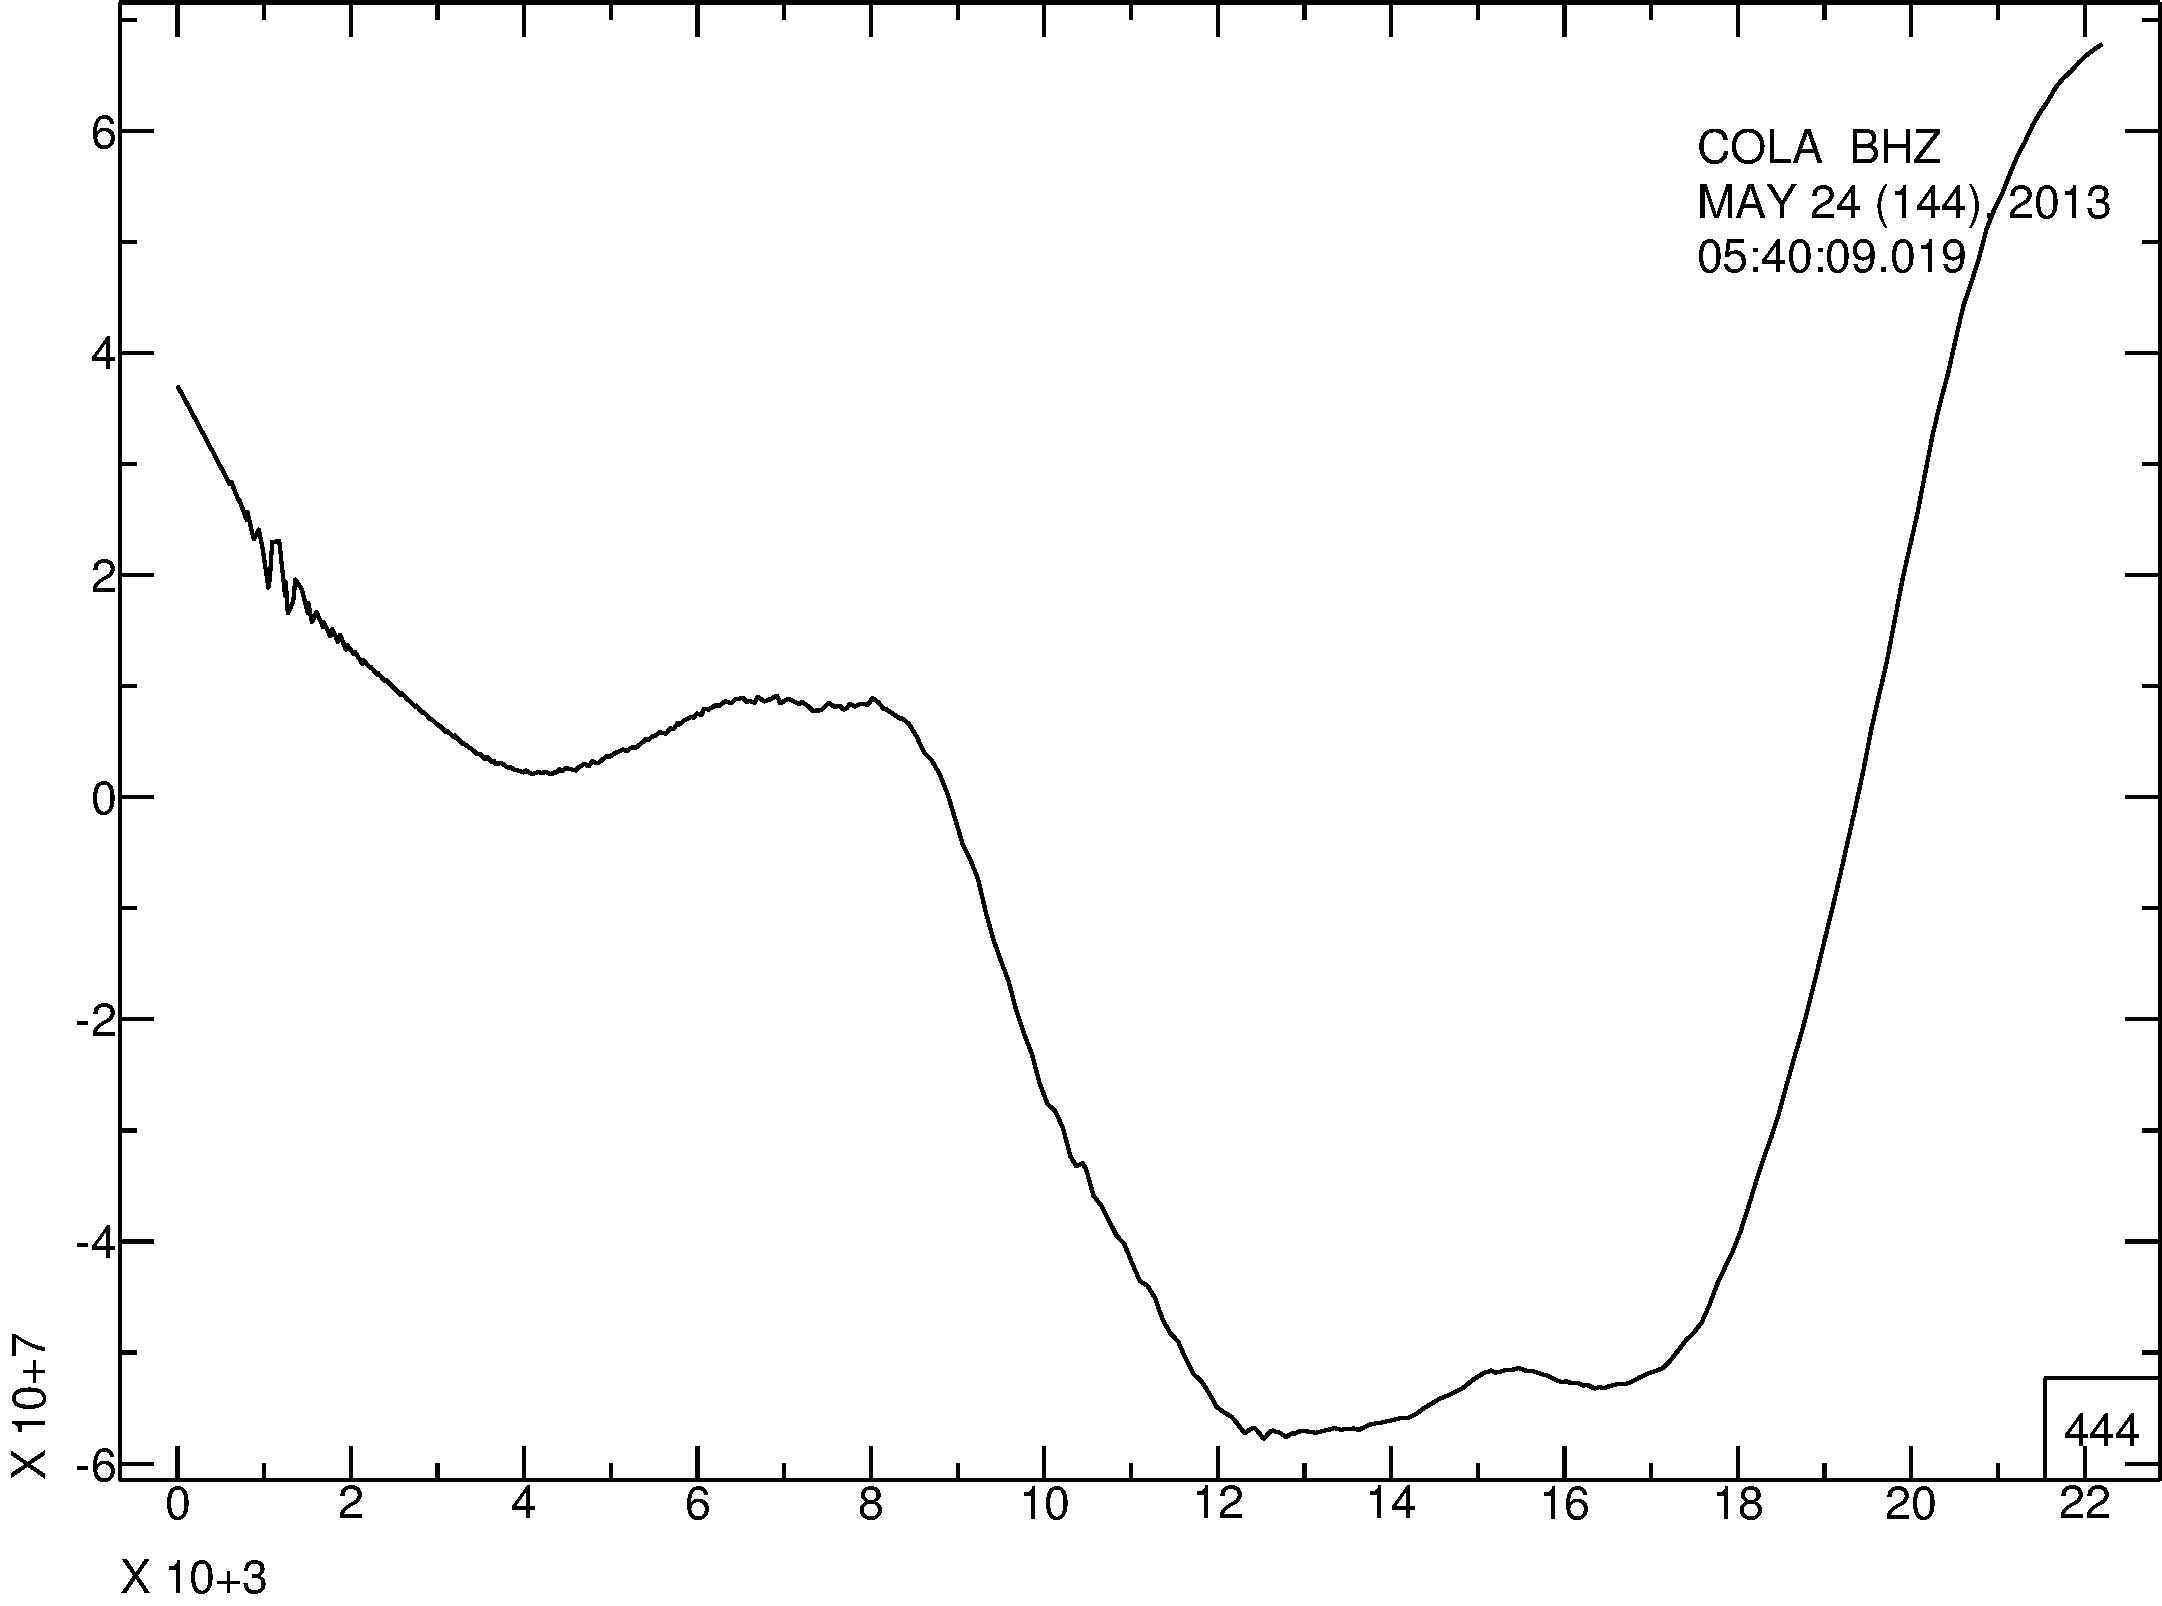
\includegraphics[width=0.98\textwidth]{ground-motion}
\caption{COLA台站处的原始地面运动}
\label{fig:ground-motion}
\end{figure}

从信号处理的角度来看,常见的地震仪是一个带通滤波器,对地震学不关心的超高频和超低频
的信号进行压制,只保留感兴趣的周期段。下图给出了该台站的仪器响应,即$i(t)$:

\begin{figure}[H]
\centering
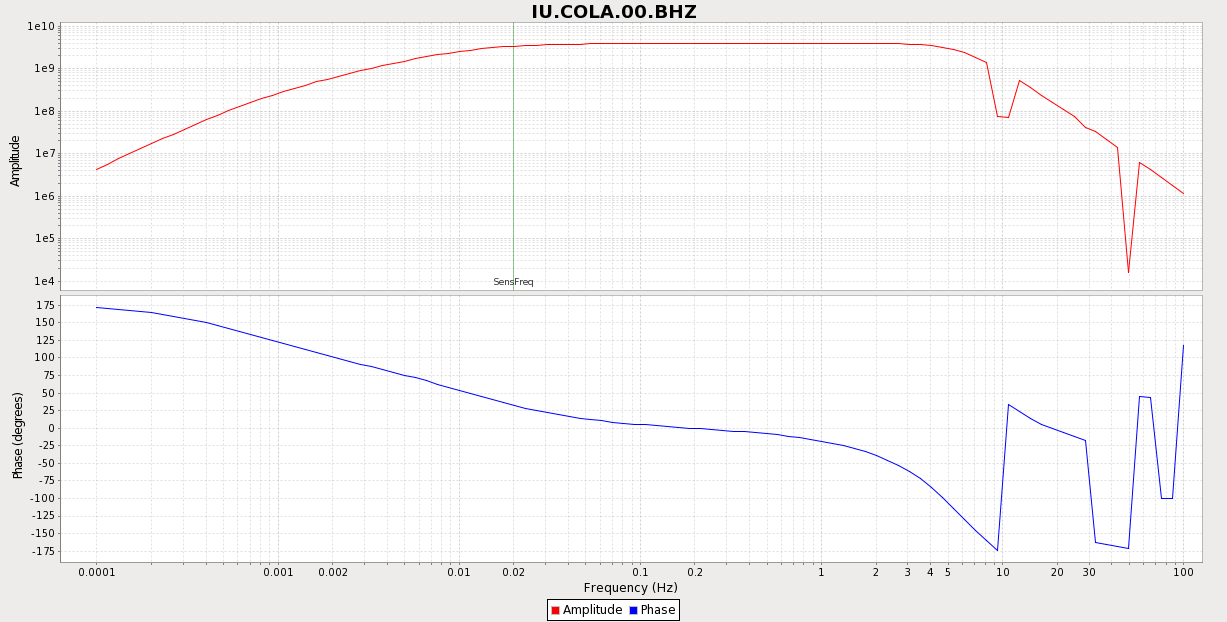
\includegraphics[width=0.98\textwidth]{transfer-function}
\caption{仪器响应频谱图}
\label{fig:transfer-function}
\end{figure}

\begin{figure}[H]
\centering
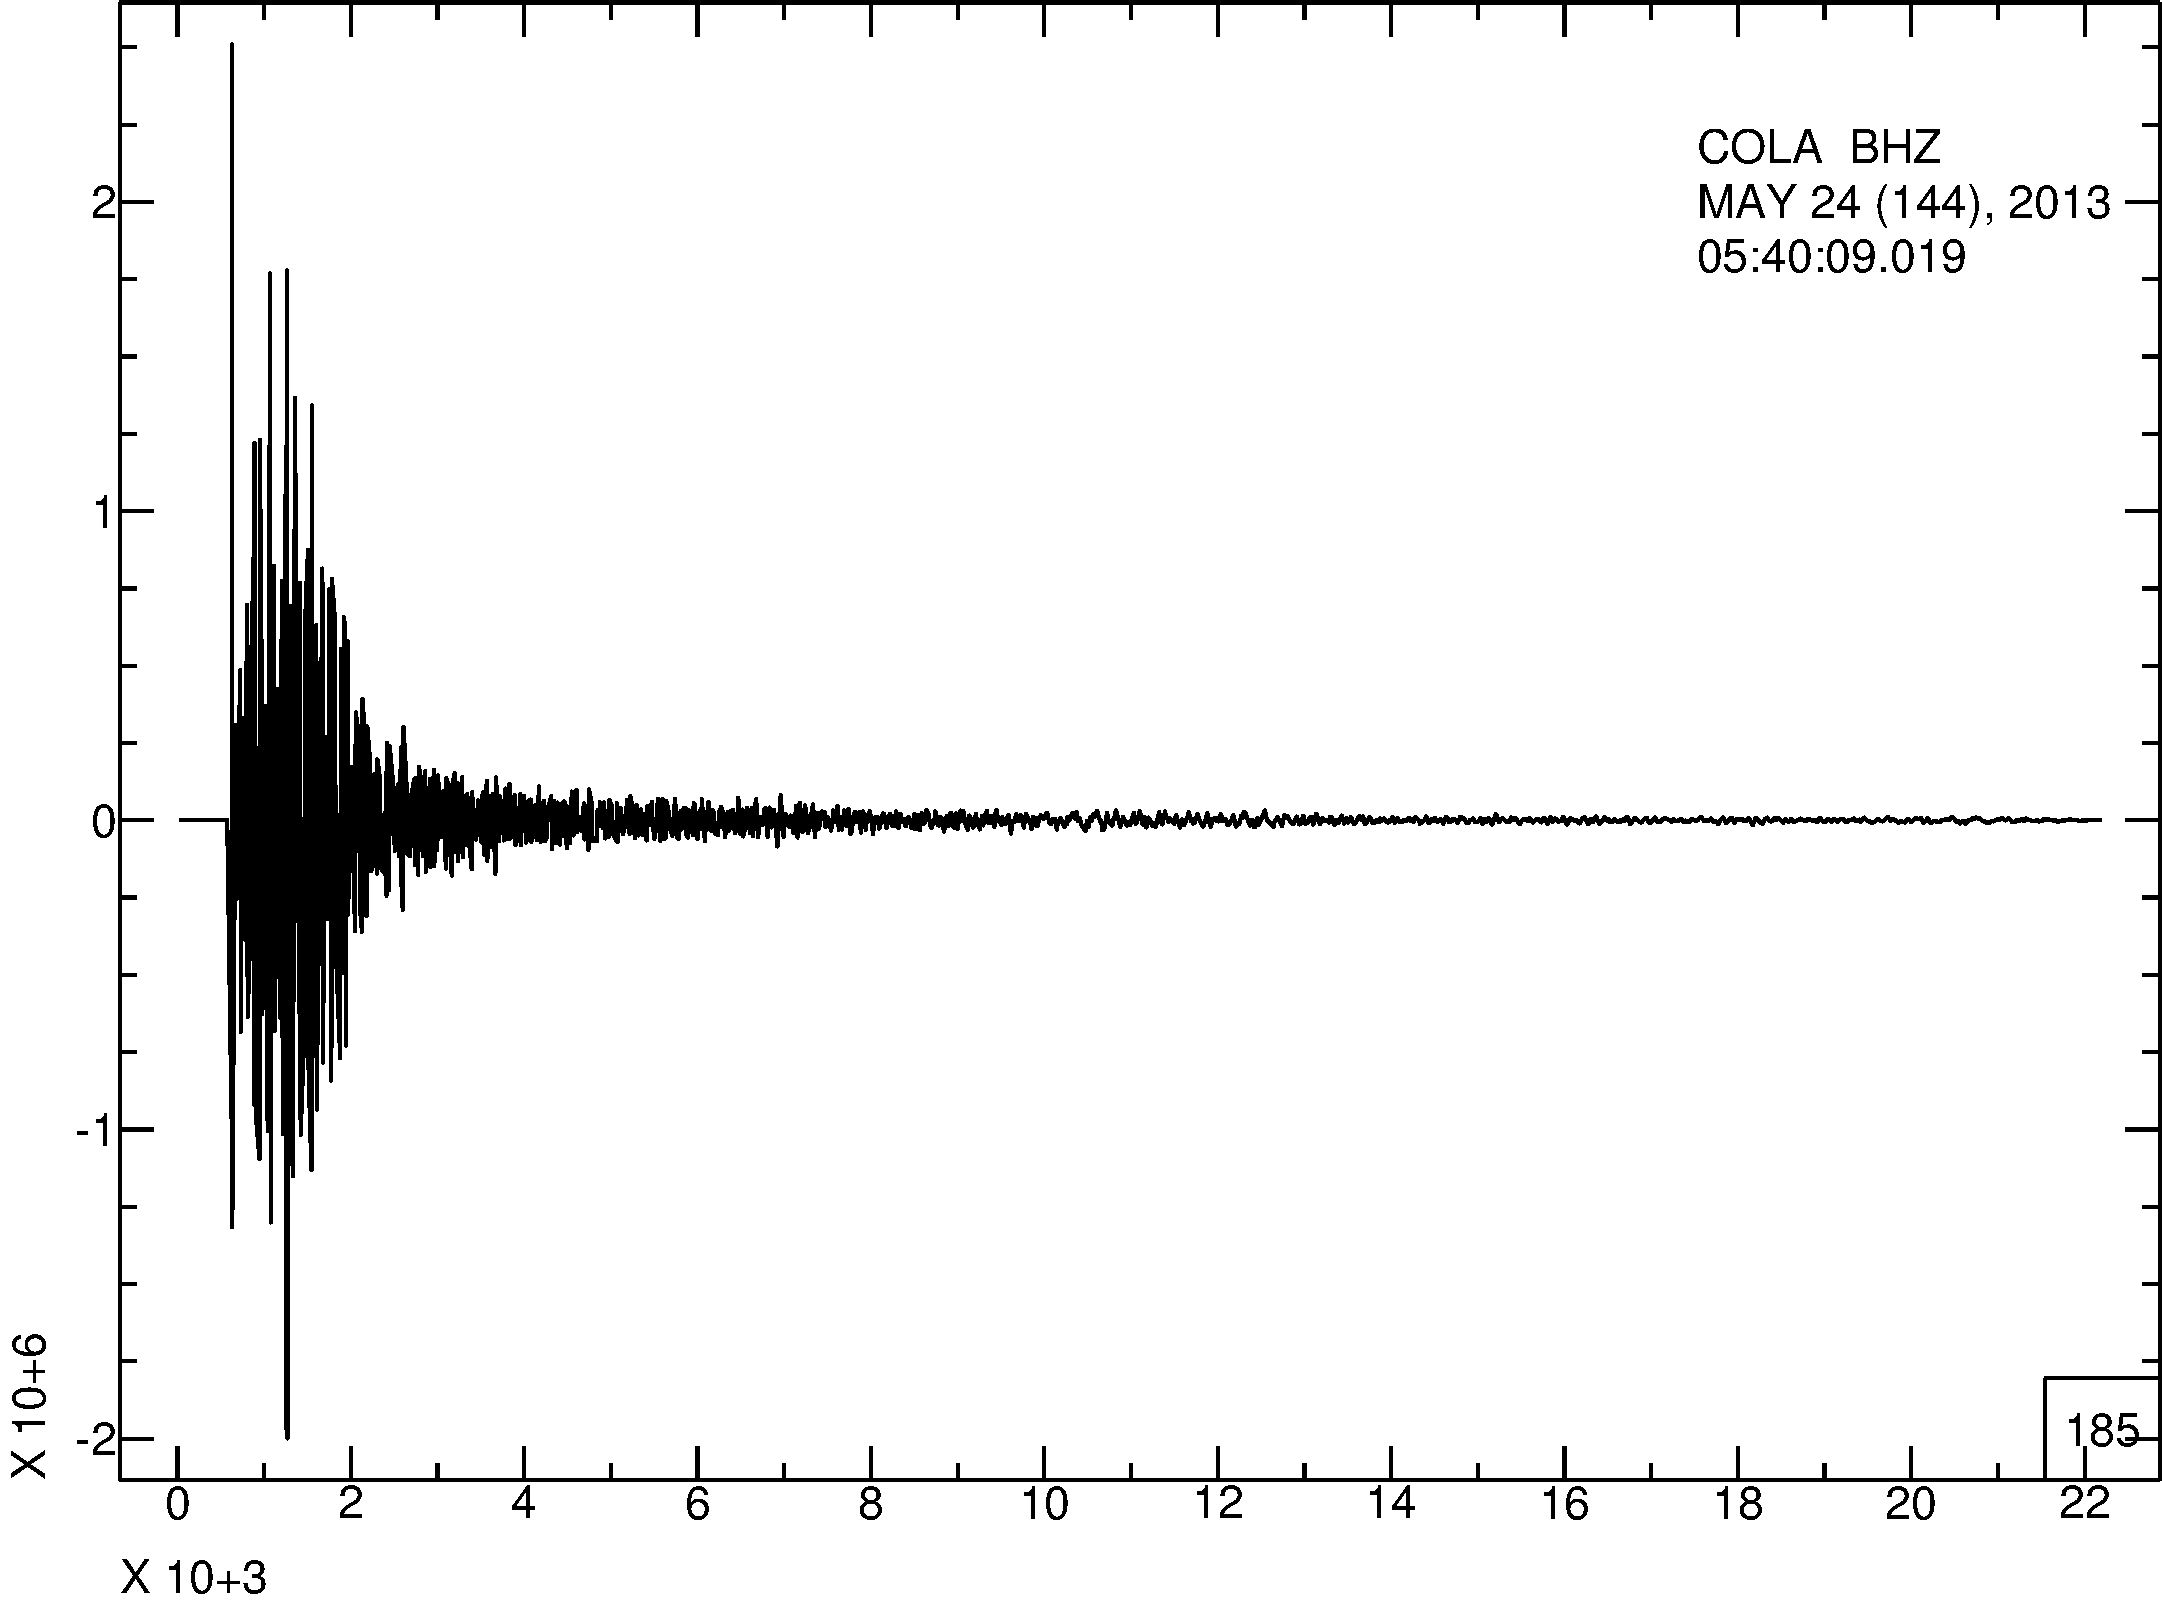
\includegraphics[width=0.9\textwidth]{raw-data}
\caption{COLA台站的地震记录}
\end{figure}

从图 \ref{fig:transfer-function} 中振幅谱可以看出,频率在 \SI{0.02}{\Hz}
到 \SI{8}{\Hz} 内的信号具有相同的振幅增益(被增强),而小于 \SI{0.02}{\Hz}
或大于 \SI{8}{\Hz} 的信号则被压制。图 \ref{fig:ground-motion} 中的周期为
\SI{1000}{\s} 量级的信号被压制到了原来的千分之一。

原始的地面运动$s(t)*g(t)$在经过仪器$i(t)$之后,即得到地震仪的数字记录,如下图。
超低频和超高频的信号被压制,留下地震学感兴趣的频段,也就是前面说的$u(t)$:

与图 \ref{fig:ground-motion} 相比,长周期的类正弦信号没了。
在 \SI{0}{\s} 到 \SI{300}{\s} 内,``地面''很安静,\SI{300}{\s} 左右,强烈的地震信号开始出现,
最大振幅约为 \num{2.4e6},持续了很长一段时间后,又恢复了``平静''。
这里可以很明显地看到``平静$\rightarrow$震动$\rightarrow$平静''的过程。这才是地震数据处理理想的波形。

为什么要去仪器响应呢?哪些时候需要去仪器响应呢?下面列举出若干需要去仪器响应的场景:
\begin{itemize}
\item 需要获取某个台站绝对振幅值;
\item 仪器响应不同的台站之间的波形对比;
\item 待补充...
\end{itemize}

\section{物理与数学}
地震仪一般固定在地表或地下浅层,也有放置在钻孔深处或海底的,因而地震仪
可以直接感知到地面的运动。在地面运动物理量被地震仪接收后,首先要将其转
换为电信号,然后对电信号振幅进行放大以及滤波,再将连续的时间序列离散化,
最终以我们常见的波形数据的形式表现出来。

概括地说,地面的运动在被地震仪感知之后,需要经历如下三个阶段,最终成为
我们拿到的波形数据:
\begin{enumerate}
\item 模拟信号阶段
\item 模数转换
\item 数字信号阶段
\end{enumerate}

地震仪的仪器响应可以表示为频率的复函数,即常说的振幅响应和频率响应。上面提到的三个阶段,每个阶段的响应函数都是频率的复函数,表示为$G_i(f)$,整个仪器的响应函数是各个阶段响应函数的乘积:
\[
    G(f)=\prod_i G_i(f)
\]

\subsection{预备知识}
在介绍地震仪的三个阶段之前,需要先了解一些基础的数学知识。
\subsubsection{响应函数}
模拟信号的响应函数用Laplace变换表示:
\[
    H(s)=\int_0^{\infty}h(t)e^{-st}dt
\]

数字信号的响应函数用Z变换表示:
\[
    H(z)=\sum_{-\infty}^{+\infty}h_m z^{-m}
\]

\subsubsection{归一化}
频率响应可以表示为
\[
    G(f)=S_d R(f)
\]
其中$R(f)$是频率的函数。在某个特定的频率$f_s$,有$|R(f_s)|=1.0$,即$R(f)$在频率$f_s$处进行归一化。$S_d$是放大系数,也称为Sensitivity或者Gain。

R(f)可以表示为
\[
    R(f)= A_0 H_p(s)
\]
其中$H_p(s)$是用零极点表示的transfer函数,一般来说在频率$f_s$处这个transfer函数的振幅响应不为1,所以需要归一化因子$A_0$。

\subsubsection{FIR滤波器}
FIR滤波器从数学上看就是对数据采样点做加权平均,设计不同的加权系数就得到不同的FIR滤波器。FIR滤波器一般设计为振幅响应为方阶跃函数(boxcar),因而其在通带内有较平的振幅响应,在拐角频率处有很尖锐很陡峭的振幅响应变化。与此同时,滤波器具有线性相位,在时间域造成信号的时间延迟,一般数据采集系统会对这个时间延迟做校正。因此,用户基本不需要考虑FIR滤波器对仪器响应的影响。

\subsection{模拟信号阶段}
模拟信号阶段会将连续的地面运动物理量(比如速度)转换为连续的电压信号,并进行电压放大。
因而此阶段的输入单位是运动物理量的单位(比如~\verb+m/s+),输出单位是伏特(\verb+V+)。

这个阶段的响应函数可以表示为
\[
    G(f)=S_d A_0 \frac{\prod_{i=1}^{n} (s-r_i)}{\prod_{j=1}^{n} (s-p_j)}=S_d A_0 H_p(s)
\]

其中,$S_d$是放大系数,$H_p(s)$是用零极点表示的transfer函数,这里有n个零点和m个极点。$A_0$是归一化因子,且$s=i 2\pi f$。

假定某仪器的自然频率为$f_0=1$ Hz, 阻尼常数为$\lambda=0.7$。如果该仪器是一个相对简单的仪器,则该仪器的加速度传递函数为:

\[
    H(s) = \frac{s}{s^2+2\lambda \omega_0 s + \omega_0^2}
\]

几点说明:
\begin{itemize}
\item 该传递函数仅表示某一类地震仪的传递函数,现代地震仪的传递函数可能比这个要复杂;
\item 根据该传递函数,很容易计算出它的一个零点和两个极点;
\end{itemize}

已知该仪器在$f_s=1$ Hz时的增益为$Sd=150 V/m \cdot s^{-2}$,即若仪器接收到1Hz频率的加速度$1 m/s^2$,则仪器的输出电压为150V。因而仪器真实的传递函数还需要把增益加进去:

\[
    G(f) = R(f)*S_d = A_0*H_p(s)*S_d
\]

其中$A_0$是归一化因子,保证在频率$f=f_s$处有$|R(f_s)|=1.0$。

\subsection{模数转换}
模数转换器,将上一阶段产生的连续电压信号转换为离散的电压信号。输入的单位是伏特~\verb+V+,输出单位是~\verb+counts+。
这个阶段,所有频段有相同的振幅响应,即只存在一个放大系数,同时可能存在一个时间延迟。

假设模数转换器是$m$位,电压范围是$\pm n V$,那么$1conuts=\frac{2n}{2^m} V$,电压也能精确到$\frac{2n}{2^m} V$。
例如,24位模数转换器的输入电压范围是$\pm 20 V$,则输出的最大范围是$\pm 2^{23}$。因而ADC的放大系数为
\[
    S_d = \frac{2^{24}}{40} = 4.1943*10^{5} counts/V
\]
即若ADC接收到的输入电压为1V,则其输出为$4.1983*10^5$ counts。结合地震仪的放大系数可知,1Hz频率的$1 m/s^2$的地面运动加速度在ADC的输出为:

\[
    1 m/s^2 * 150 \frac{V}{m/s^2} * 4.1943\times 10^5 \frac{counts}{V} = 6.29145*10^7 counts
\]

另一方面,ADC的输入电压上限为20V,因而仪器所能记录的最大加速度为$20/150=0.13 m/s^2$。

\subsection{数字信号阶段}
这个阶段会对数据信号进行进一步的处理,主要包含三个部分,即离散信号滤波、数据重采样、时间延迟校正。

离散信号滤波可以采用FIR滤波器,也可以采用IIR滤波器。多数情况下采用FIR滤波器,而FIR滤波器的振幅响应函数可以认为在全频段内为1
\footnote{FIR滤波器在Nyquist频率附近会有5\%左右的震荡,因而若感兴趣的频率与Nyquist频率相差较大,则可以忽略这一阶段的响应函数},因而这个阶段只需要考虑放大系数,而不需要再考虑由于滤波引入的响应函数。同样,对于数据重采样以及时间校正也不会引入新的响应函数。

\subsection{小结}
综上所述,三个阶段中,第一个阶段最为复杂,需要给出放大系数$Sd_{1}$、归一化因子$A_0$以及零极点信息;第二个阶段以及第三个阶段都只需要给出放大系数$Sd_{2}$和$Sd_3$。最终得到仪器的响应函数为
\[
    G(f)=Sd_1 A_0 H_p(s) Sd_2 Sd_3=Sd_0 A_0 H_p(s)
\]
即需要仪器在第一个阶段的零极点信息、归一化因子$A_0$以及三个阶段的放大系数的乘积$Sd_0$即可以近似表示地震仪的仪器响应。

\section{仪器响应文件}
在SAC诞生的80年代,模拟地震仪的类型很少,SAC将这些地震仪器的响应函数都内置到
程序中,可以直接使用。随着数字地震仪的出现和不断发展,地震仪器的类型越来越丰富,
不可能把这些地震仪器的响应函数都内置到SAC中,这就需要有更通用的方式来描述仪器响应,
即仪器响应文件:RESP、PZ和FAP。

\subsection{内置仪器响应}
SAC内置了很多标准地震仪器的仪器响应,如表 \ref{table:instrument-type} 所示。
部分仪器类型还拥有子类型,如表 \ref{table:instrument-subtype} 所示。在SAC命令中,
可以直接使用这些仪器类型。

\begin{table}[tp]
\centering
\ttfamily
\small
\caption{SAC内置仪器类型列表}
\label{table:instrument-type}
\begin{tabular}{ll}
\toprule
type     &  说明  \\
\midrule
BBDISP   &  Blacknest specification of Broadband Displacement \\
BBVEL    &  Blacknest specification of Broadband Velocity   \\
BENBOG   &  Blacknest specification of Benioff by Bogert    \\
DSS      &  LLNL Digital Seismic System \\
DWWSSN   &  Digital World Wide Standard Seismograph Station \\
EKALP6   &  Blacknest specification of EKA LP6  \\
EKASP2   &  Blacknest specification of EKA SP2  \\
ELMAG    &  Electromagnetic \\
GBALP    &  Blacknest specification of GBA LP   \\
GBASP    &  Blacknest specification of GBA SP   \\
GENERAL  &  General seismometer \\
GSREF    &  USGS Refraction \\
HFSLPWB  &  Blacknest specification of HFS LPWB \\
IW       &  EYEOMG-spectral differentiation \\
LLL      &  LLL broadband analog seismometer    \\
LLSN     &  LLSN L-4 seismometer    \\
LNN      &  Livermore NTS Network instrument    \\
LRSMLP   &  Blacknest specification of LRSM LP  \\
LRSMSP   &  Blacknest specification of LRSM SP  \\
NORESS   &  NORESS (NRSA)   \\
NORESSHF &  NORESS high frequency element   \\
OLDBB    &  Old Blacknest specification of BB   \\
OLDKIR   &  Old Blacknest specification of Kirnos   \\
PORTABLE &  Portable seismometer with PDR2  \\
PTBLLP   &  Blacknest specification of PTBL LP  \\
REDKIR   &  Blacknest specification of RED Kirnos   \\
REFTEK   &  Reftek 97-01 portable instrument    \\
RSTN     &  Regional Seismic Test Network   \\
S750     &  S750 Seismometer    \\
SANDIA   &  Sandia system 23 instrument \\
SANDIA3  &  Sandia new system with SL-210   \\
SRO      &  Seismic Research Observatory    \\
WA       &  Wood-Anderson   \\
WABN     &  Blacknest specification of Wood-Anderson    \\
WIECH    &  Wiechert seismometer    \\
WWLPBN   &  Blacknest specification of WWSSN long period    \\
WWSP     &  WWSSN short period  \\
WWSPBN   &  Blacknest specification of WWSSN short period   \\
YKALP    &  Blacknest specification of YKA long period  \\
YKASP    &  Blacknest specification of YKA short period \\
\bottomrule
\end{tabular}
\end{table}

\begin{table}[htb]
\centering
\ttfamily
\small
\caption{部分仪器子类型}
\label{table:instrument-subtype}
\begin{tabular}{ll}
\toprule
主类型 &   子类型 \\
\midrule
LLL       &       LV, LR, LT, MV, MR, MT, EV, ER, ET, KV, KR, KT    \\
LNN       &       BB|HF                                 \\
NORESS    &       LP|IP|SP                              \\
RSTN      &       [CP|ON|NTR|NY|SD][KL|KM|KS|7S][Z|N|E] \\
SANDIA    &       [N|O][T|L|B|D|N|E][V|R|T]             \\
SRO       &       BB|SP|LPDE                            \\
FREEPERIOD v &    ELMAG, GENERAL, IW, LLL SUBTYPE BB, REFTEK    \\
MAGNIFICATION n & ELMAG, GENERAL  \\
NZEROS n &        GENERAL, IW   \\
DAMPING v &       GENERAL, LLL SUBTYPE BB, REFTEK   \\
CORNER v &        LLL SUBTYPE BB, REFTEK    \\
GAIN v &            \\
HIGHPASS v &      REFTEK    \\
\bottomrule
\end{tabular}
\end{table}

除了表 \ref{table:instrument-type} 中列出的众多仪器类型之外,还有几个特别的仪器类型:
\begin{itemize}
\item none:即位移,也是SAC的默认值
\item vel:速度
\item acc:加速度
\end{itemize}

\subsection{RESP文件}
RESP文件是用于描述仪器响应的文件,其包含了描述仪器响应所需要的全部信息。

RESP仪器响应文件可以通过如下几种方式获得:
\begin{itemize}
\item 用rdseed程序从SEED数据中提取;
\item 用evalresp程序从SEED数据中提取;
\item 从IRIS DMC resp Web Service\footnote{\url{http://service.iris.edu/irisws/resp/1/}}下载;
\item 手写RESP文件;
\end{itemize}

一个RESP文件中可以只包含一个仪器响应函数,也可以包含多个台站、多通道、多时间段的
多个仪器响应函数。每个仪器响应函数中包含了台站名、台网名、通道名、开始时间和结束
时间等台站的基本信息。具体的仪器响应函数部分又分成多个Stage,每个Stage中又分为多
个block,包含了仪器响应的不同信息。

\begin{itemize}
\item Stage1一般对应模拟信号阶段,从中可以提取中这一阶段的输入单位、零极点、归一化因子$A_0$以及第一阶段的增益。
\item Stage2一般对应ADC阶段,从中可以提取出这一阶段的放大系数。
\item Stage3一般对应于数字滤波和减采样阶段。通常需要对数字信号多次滤波或减采样,因而Stage3后面可能会接多个类似的Stage。从这几个Stage中提取的信息是增益,一般值为1。
\item Stage0是会给出前面所有Stage的增益的乘积,主要是起到了辅助验证的作用。
\end{itemize}

\subsection{SAC PZ文件}
RESP文件中包含了仪器响应的完整信息,同时也包含了不少冗余信息。SAC从RESP文件中
提取处仪器响应中的重要信息,定义了新的零极点响应文件(即SAC PZ)。
相对于RESP文件而言,PZ文件中仅包含仪器响应中的零极点和增益信息,在去仪器响应时更方便。

SAC PZ文件主要通过以下几种方式获得:
\begin{itemize}
\item 用rdseed程序从SEED文件中提取;
\item 从IRIS DMC SAC PZ Web Service\footnote{\url{http://service.iris.edu/irisws/sacpz/1/}}获取;
\end{itemize}

下面是某个台站的SAC PZ文件:
\begin{verbatim}
* **********************************
* NETWORK   (KNETWK): IU
* STATION    (KSTNM): COLA
* LOCATION   (KHOLE): 00
* CHANNEL   (KCMPNM): BHZ
* CREATED           : 2013-06-22T14:12:09
* START             : 2012-09-14T04:00:00
* END               : 2599-12-31T23:59:59
* DESCRIPTION       : College Outpost, Alaska, USA
* LATITUDE          : 64.873599
* LONGITUDE         : -147.861600
* ELEVATION         : 84.0
* DEPTH             : 116.0
* DIP               : 0.0
* AZIMUTH           : 0.0
* SAMPLE RATE       : 20.0
* INPUT UNIT        : M
* OUTPUT UNIT       : COUNTS
* INSTTYPE          : Geotech KS-54000 Borehole Seismometer
* INSTGAIN          : 2.013040e+03 (M/S)
* COMMENT           : N/A
* SENSITIVITY       : 3.377320e+09 (M/S)
* A0                : 8.627050e+04
* **********************************
ZEROS   3
        +0.000000e+00   +0.000000e+00
        +0.000000e+00   +0.000000e+00
        +0.000000e+00   +0.000000e+00
POLES   5
        -5.943130e+01   +0.000000e+00
        -2.271210e+01   +2.710650e+01
        -2.271210e+01   -2.710650e+01
        -4.800400e-03   +0.000000e+00
        -7.384400e-02   +0.000000e+00
CONSTANT        +2.913631e+14
\end{verbatim}

SAC PZ文件中,以星号开始的行为注释行,给出了该PZ文件所对应的台站信息,其中
INPUT UNIT表明了该PZ文件的输入是位移、速度还是加速度。用rdseed从SEED数据中
提取出来的PZ文件,输入都是位移,且单位为 \si{\m}。

以关键字``ZEROS''起始的行给出了零点数目,接下来几行列出了
每个零点的实部和虚部。以关键字``POLES''起始的行给出了极点数目,接下来几行列出了
每个极点的实部和虚部。最后一行给出了仪器响应中的常数CONSTANT。

根据零极点以及CONSTANT,即可计算得到仪器响应函数:
\[
    H(s) = C_0 * \frac{(s-z_1)(s-z_2)...(s-z_{nz})}{(s-p_1)(s-p_2)...(s-p_{nz})}
\]
其中$s=2\pi i f$。

一些说明:
\begin{itemize}
\item 若有零点 \texttt{(0.0,0.0)},则这样的``零''零点可以省略。因而列出的零点数可能会少于``ZEROS''行给出的零点数;上例中的三个零点可以不列出;
\item CONSTANT对应于RESP文件中所有阶段的增益$Sd_0$以及归一化因子$A_0$的乘积;
\item 若未指定CONSTANT,则默认值为1.0;
\end{itemize}

\subsection{FAP文件}
FAP文件是响应函数的另一种表现形式,其包含了很多记录行,每行三个字段,
分别是频率(HZ)、振幅及相位。

频率不需要等间隔分段。在执行transfer时,低于第一行频率的频段将使用第一行的振幅和相位;
同理大于最后一行频率的频段将使用最后一行的振幅和相位。

FAP文件可以从程序evalresp v3.3.2中获得,FAP相对于PZ文件的优势在于,其给出了每个频率的
振幅和相位响应,因而包含更丰富的信息,且方便人工修改以控制需要校正的频率段。

\subsection{RESP vs PZ vs FAP}
RESP、PZ和FAP都可以用于表征仪器的响应函数,常见的是RESP和PZ,而这两种还是有很大区别的:

\begin{itemize}
\item RESP文件包含了仪器响应的完整信息,而PZ文件中仅包含了零极点
    和增益信息,二者的主要差异在于PZ文件中未包含FIR滤波器的信息;
\item RESP文件中可以知道输入数据是位移、速度还是加速度,而PZ文件默认输入
    为位移。因而若RESP文件中输入是速度,则PZ文件中会多一个``零''零点;
    若RESP文件中输入是加速度,则PZ文件中会多两个``零''零点;
\item SAC中的默认位移单位是 \si{\nm},RESP文件中有指定输入单位为 \si{\m},
    因而在用RESP去仪器响应时,transfer会在去除仪器响应之后在对数据做单位
    上的变换以使得得到的位移数据的单位是 \si{\nm},即与SAC的标准相一致。
    而PZ文件中并未提供输入单位信息,或者说即便提供了也没有被利用到,故而
    用PZ文件去除仪器响应得到的位移物理量单位是 \si{\m},为了与SAC标准相
    一致,需要对数据乘以10的9次方将数据单位由 \si{\m} 转换成 \si{\nm};
\end{itemize}

对于大多数情况,建议使用PZ文件,数据处理速度要快很多。


\chapter{数据命名规则}
\label{chap:naming}
用rdseed程序从标准SEED格式中解压得到的SAC文件,通常都具有固定格式的文件名。具体格式为:
\begin{verbatim}
    yyyy.ddd.hh.mm.ss.ffff.NN.SSSSS.LL.CCC.Q.SAC
\end{verbatim}
其中
\begin{itemize}
\item \texttt{yyyy.ddd.hh.mm.ss.ffff} 是SAC文件中第一个数据点对应的时间
    \begin{itemize}
    \item \texttt{yyyy} 为年;
    \item \texttt{ddd} 为一年的第多少天;
    \item \texttt{hh.mm.ss} 为时、分、秒;
    \item \texttt{ffff} 为毫秒;需要注意的是 $\SI{1}{\s}=\SI{1000}{\ms}$,
        这里毫秒用了4位来表示。
    \end{itemize}
\item \texttt{NN} 为台网名,2字符;
\item \texttt{SSSSS} 为台站名,一般是3个字符,偶尔见到4字符的;
\item \texttt{LL} 为location id,为空或两字符;
\item \texttt{CCC} 为通道名;
\item \texttt{Q} 为质量控制标识;
\item \texttt{SAC} 为文件后缀;
\end{itemize}

\section{Location ID}
关于Location ID,我并没有找到权威的解释。

常见的Location ID为空值,非空值一般常见到 \texttt{00}、\texttt{01}、\texttt{10},
偶尔也会见到 \texttt{60} 等。

Location ID可以认为是台站的subcode,即一个台站处,有多套仪器,这些仪器可能
是相同的型号,但是位于不同的深度或者指向不同的方位;也有可能是不同型号的仪器。

\section{质量控制}
质量控制符Q用于表征当前SAC数据的数据质量。该标识符可以取如下四种:
\begin{itemize}
\item \texttt{D} 不确定状态的数据
\item \texttt{M} 已合并的数据
\item \texttt{R} 原始波形数据
\item \texttt{Q} 经过质量控制的数据
\end{itemize}
常见的数据标识符为H或Q。

\section{通道名}
通道名用三个字符来表示,这三个字符分别代表了Band Code、Instrument Code和Orientation Code。

\subsection{Band Code}
Band Code是通道名的第一个字符,表示了仪器的采样率以及响应频带等信息。

\begin{table}[H]
\centering\small
\caption{Band Code}
\label{tbl:bandcode}
\begin{tabular}{cllc}
\toprule
Band Code   &   Band Type   &   Sample rate (Hz)    & Corner peroid (sec)   \\
\midrule
F           &   ...         &   1000-5000   &     > 10    \\
G           &   ...         &   1000-5000   &     < 10    \\
D           &   ...         &   250-1000    &     < 10    \\
C           &   ...         &   250-1000    &     > 10    \\
E           &   Extremely Short Period  & 80-250    &     < 10    \\
S           &   Short Period          & 10-80   & < 10    \\
H           &   High Broad Band         &   80-250    &   < 10    \\
B           &   Broad Band          &   10-80   & > 10    \\
M           &   Mid Period          &   1-10   & > 10    \\
L           &   Long Period         &   $\approx$ 1   &   \\
V           &   Very  Long Period         & $\approx$ 0.1   &   \\
U           &   Ultra Long Period         & $\approx$ 0.01    &   \\
R           &   Extremely Long Period     & 0.0001-0.001    &   \\
P           &   Order of 0.1 to 1 days   & 0.00001-0.0001    &   \\
T           &   Order of 1 to 10 days    & 0.000001-0.00001    &   \\
Q           &   Greater than 10 days          &     < 0.000001    &   \\
Q           &   Administrative Instrument Channel   & variable    & NA    \\
O           &   Opaque Instrument Channel         & variable    &   NA    \\
\bottomrule
\end{tabular}
\end{table}
常见的仪器一般是宽频带(B)或长周期(L)。

\subsection{Instrument Code}
Instrument Code是通道名的第二个字符,代表了不同的仪器传感器。
\begin{table}[H]
\centering
\caption{Instrument Code}
\begin{tabular}{cl}
\toprule
Instrument Code    &     说明   \\
\midrule
H        &       High Gain Seismometer      \\
L        &       Low Gain Seismometer       \\
G        &       Gravimeter                 \\
M        &       Mass position Seismometer  \\
N        &       Accelerometer              \\
\bottomrule
\end{tabular}
\end{table}
常见的是高增益(H)仪器,记录地面运动速度。

\subsection{Orientation Code}
Orientation Code表示了传感器记录的地面运动的方向。
\begin{table}[H]
\centering
\caption{Orientation Code}
\begin{tabular}{cl}
\toprule
Code     &     说明   \\
\midrule
N E Z   &   南北向、东西向、垂向   \\
1 2 3   &   3为垂向;1、2为水平方向,正交但与东西南北向有偏离   \\
T R Z   &   切向、径向,主要用于射线束中    \\
A B C   &   三轴向(正交)    \\
U V W   &   可选分量    \\
\bottomrule
\end{tabular}
\end{table}
常见的是N、E、Z以及1、2、3。

需要注意的是:当仪器的方向与东西方向的夹角小于5度时,Orientation Code取为E;
当与东西方向夹角大于5度时,Orientation Code取为1(或2)。对于南北方向同理。
因而,即便Orientation Code为N,也并不意味着台站是南北方向的,真实的方向还是
需要看SAC头段中的cmpaz和cpminc。

\chapter{数据获取}
\section{数据来源}
地震波形数据的来源有很多,下面列举并简单介绍常见的数据来源。

\subsection{国家测震台网数据备份中心}
\href{http://www.seisdmc.ac.cn/}{国家测震台网数据备份中心},隶属于
中国地震局地球物理研究所。到2014年底,国家测震台网已建成由170个台站
和3个小孔径台阵(共30个子台)组成的国家地震台网;859个台站组成的31个
区域地震台网,33个子台组成的6个火山监测台网;291套地震仪器组成的32个
应急流动观测台网。国家测震台网数据备份中心可以提供从2007年8月起的
全球M5.5级以上地震事件以及国内及周边地区M3.5级以上地震事件的波形数据。

要申请数据备份中心的数据,需要注册账户并升级账户属性。
要升级账户属性,需要按程序进行申请,并且签署和遵守
\href{http://www.seisdmc.ac.cn/class/view?id=8}{相关协议}。

\subsection{IRIS DMC}
\label{subsec:IRIS}
\href{http://ds.iris.edu/ds/nodes/dmc/}{IRIS DMC} 是世界上最大的地震
波形数据中心。

IRIS DMC的大部分数据是完全公开的,无需注册即可直接申请下载波形数据。
从IRIS DMC申请数据的工具有很多:
\href{https://ds.iris.edu/ds/nodes/dmc/manuals/breq_fast/}{BREQ\_FAST}、
\href{http://ds.iris.edu/wilber3/find_event}{Wilber III}、
\href{http://service.iris.edu/}{Web Service}、
\href{http://ds.iris.edu/ds/nodes/dmc/software/downloads/irisfetch.m/}{irisfetch.m}、
\href{https://seiscode.iris.washington.edu/projects/ws-fetch-scripts}{Web Service Fetch scripts}、
\href{http://www.seis.sc.edu/sod/}{SOD} 和
\href{https://ds.iris.edu/ds/nodes/dmc/software/downloads/jweed/}{JWEED}。

\subsection{NIED}
\label{subsec:NIED}
\href{http://www.bosai.go.jp/}{NIED}是日本的国家防灾科学技术研究所。其
下包含若干台网:高感度地震观测网 \href{http://www.hinet.bosai.go.jp/}{Hi-net}、
宽频带地震台网 \href{http://www.fnet.bosai.go.jp/}{F-net}、强地面运动地震
台网 \href{http://www.kyoshin.bosai.go.jp/}{K-net和KiK-net} 和
火山观测网 \href{http://www.vnet.bosai.go.jp/}{V-net}。

\subsection{Natural Resources Canada}
\label{subsec:nrcan}
加拿大政府的网站 \href{http://www.nrcan.gc.ca/home}{Natural Resources Canada}
提供了
\href{http://www.earthquakescanada.nrcan.gc.ca/stndon/CNSN-RNSC/index-eng.php}{Canadian National Seismic Network}、
\href{http://can-ndc.nrcan.gc.ca/yka/index-en.php}{Yellowknife Seismic Array}、
POLARIS Network等台网/台阵的连续波形数据以及这些台网/台阵1975年至今的事件
波形数据。

事件波形数据可以直接 \href{http://www.earthquakescanada.nrcan.gc.ca/stndon/NWFA-ANFO/eve/index-eng.php}{点击下载};
连续波形数据则可以通过工具
\href{http://www.earthquakescanada.nrcan.gc.ca/stndon/AutoDRM/index-eng.php}{AutoDRM} 下载。

\subsection{其他}
\begin{itemize}
\item \href{http://www.ncedc.org/}{Northern California Earthquake Data Center}
\item \href{http://pnsn.org/}{Pacific Northwest Seismic Network}
\item \href{http://www.scsn.org/}{Southern California Seismic Network}
\item \href{http://scedc.caltech.edu/}{Southern California Seismic Network at Caltech}
\item \href{http://www.chinarraydmc.org/}{中国地震科学探测台阵数据中心}
\end{itemize}

\section{IRIS地震数据申请工具}
从IRIS申请地震波形数据时,有很多工具可供选择与使用。这一节不会去介绍工具
的具体用法,而是试着总结不同工具各自的优缺点以及适用范围。读者应根据实际
需求选择合适的工具,并自行阅读相应工具的说明文档。

\subsection{Wilber III}
主页:\url{http://ds.iris.edu/wilber3/find_event}

教程:\url{http://seisman.info/wilber3.html}

\begin{itemize}
\item 适用范围:仅用于申请基于事件的事件波形数据
\item 特色及优点:
    \begin{itemize}
    \item 网页端
    \item 提供地震目录,筛选条件:经纬度范围、发震时刻、震级范围
    \item 基于Google地图服务显示地震分布
    \item 台站筛选条件:台网名、虚拟台网名、通道名、震中距范围、方位角范围
    \item 基于Google地图服务显示台站分布
    \item 提供波形预览
    \item 根据发震时刻、P波到时、S波到时确定数据时间窗
    \item 数据格式:SAC、SEED、miniSEED、ASCII、dataless SEED
    \item 申请得到的数据位于IRIS的FTP中
    \item 申请得到的数据已经写入事件信息
    \end{itemize}
\item 缺点:
    \begin{itemize}
    \item 一次只能下载一个事件的波形数据,难以自动化
    \item 只能用于基于事件的波形数据,无法用于基于台站的波形数据或
        连续波形数据
    \end{itemize}
\end{itemize}

\subsection{BREQ\_FAST}
主页:\url{https://ds.iris.edu/ds/nodes/dmc/manuals/breq_fast/}

教程:\url{http://seisman.info/iris-breq-fast.html}

\begin{itemize}
\item 适用范围:连续波形数据
\item 特色及优点:
    \begin{itemize}
    \item 发送特定格式的邮件到特定邮箱即可申请数据
    \item 邮件格式相对简单
    \item 易于自动化和批量处理
    \item 数据格式:发送到不同的邮箱可分别得到SEED、miniSEED和
        dataless格式的数据
    \item 申请的数据位于IRIS的FTP里
    \end{itemize}
\item 缺点:需要一定的编程基础
\end{itemize}

\subsection{DMC Web Service}
主页:\url{http://service.iris.edu/fdsnws/dataselect/1/}

\begin{itemize}
\item 适用范围:连续波形数据
\item 特色及优点:
    \begin{itemize}
    \item 基于Web的服务,是其他多个工具的基础
    \item 按照固定的格式构建一个URL贴到浏览器中即可申请相应的数据
    \item 数据格式:miniSEED
    \end{itemize}
\item 缺点:Web服务太原始,仅在个别情况下比较适用,大多数情况下都需要
    编程调用该服务
\end{itemize}

\subsection{JWEED}
主页:\url{https://ds.iris.edu/ds/nodes/dmc/software/downloads/jweed/}

\begin{itemize}
\item 适用范围:基于事件的事件波形数据+基于台站的事件波形数据
\item 特色及优点:
    \begin{itemize}
    \item Java语法写的GUI客户端
    \item 基于DMC Web Service
    \item 跨平台,但兼容性较差,某些平台下无法正常使用
    \item 运行速度稍慢
    \item 地震目录类型:NEIC PDE、GCMT、ISC、ANF
    \item 地震事件筛选条件:时间范围、震级范围、深度范围
    \item 台站筛选条件:台网名、虚拟台网名、通道名
    \item 地震台站对筛选条件:方位角范围、反方位角范围、震中距范围
    \item 数据格式:SAC、RESP、PZ、ASCII、miniSEED
    \item 可以生成 \verb|BREQ_FAST| 格式的文件,供发邮件申请数据
    \item 数据会直接下载保存到本地
    \end{itemize}
\item 缺点:无法下载连续数据
\end{itemize}

\subsection{Web Service fetch scripts}
主页:\url{https://seiscode.iris.washington.edu/projects/ws-fetch-scripts}

\begin{itemize}
\item 适用范围:连续波形数据
\item 特色及优点:
    \begin{itemize}
    \item Perl语言写的脚本,在命令行使用
    \item 基于DMC Web Service
    \item 数据格式:miniSEED
    \end{itemize}
\item 缺点:仅适用于连续波形数据。相对于原始的Web Service的优点在于,
    可编程实现批量申请
\end{itemize}

\subsection{irisfetch.m}
主页:\url{https://ds.iris.edu/ds/nodes/dmc/software/downloads/irisfetch.m/}

\begin{itemize}
\item 适用范围:连续波形数据
\item 特色及优点:
    \begin{itemize}
    \item Matlab脚本,可以在Matlab中直接调用相关函数获取数据
    \item 基于DMC Web Service
    \item 数据格式:保存为Matlab自定义结构体
    \end{itemize}
\end{itemize}

\subsection{SOD}
主页:\url{http://www.seis.sc.edu/sod/}

\begin{itemize}
\item 适用范围:基于事件的事件波形数据+基于台站的事件波形数据
\item 特色及优点:
    \begin{itemize}
    \item 命令行工具,易于批量处理
    \item 申请数据的同时可以对数据进行预处理
    \item 数据格式:SAC、miniSEED
    \end{itemize}
\item 缺点:学习成本较高
\end{itemize}


\chapter{文档更新与维护}
\label{chap:doc-maintenance}
\section{手册简介}
《SAC参考手册》(也就是你正在阅读的文档)是一本详细介绍SAC用法的中文电子书。

2011年暑假,seisman用20天左右的时间翻译了官方的英文帮助文档;
2012年初将翻译的文档整理成PDF并发布1.0版;
2013年3月用 \LaTeX 重新对文档做了排版并发布2.0版;
2014年4月重新设计了整个文档的结构并重写了文档的大部分内容,并发布3.0版;
目前,文档依旧在不断更新中。

该手册的源码使用 \LaTeX ,并开源托管在GitHub上:
\begin{itemize}
\item 项目主页:\url{https://github.com/seisman/SAC_Docs_zh}
\item 文档发布页:\url{http://seisman.info/sac_manual.html}
\end{itemize}

\section{文档更新历史}
\subsection*{2012-01-08 1.0版}
\begin{itemize}
\item 第一版发布,由DOC转换为PDF
\item 参考《数字地震波形分析》一书,翻译了大部分官方文档中的内容
\item 结合SAC 101.4版本,增加、删除和修改了一些命令
\item 增加了书签,方便定位,支持全文搜索
\end{itemize}

\subsection*{2012-09-03 1.1版}
\begin{itemize}
\item 重新格式化整个文档,使得其看上去更规范,也易于以后的修改
\item 代码从NotePad++中直接导出,支持语法高亮
\item 代码及正文英文字体采用Consolas字体
\item 增加了``在脚本中调用SAC''一节
\item 新增命令 \texttt{transfer}、\texttt{traveltime}、\texttt{saveimg}、\texttt{datagen}
\item 更新至SAC v101.5c
\item 公式用公式编辑器编辑
\end{itemize}

\subsection*{2012-09-18 1.2版}
\begin{itemize}
\item 增加了封面配图
\end{itemize}

\subsection*{2013-03-29 2.0版}
用 \LaTeX 重新排版文档
\begin{itemize}
\item 操作系统:CentOS 6.4
\item 编译环境:\TeX~Live~2012
\item 编译命令:XeLaTeX
\item 中文实现:\CTeX 宏包
\item 中文字体:宋体+黑体
\item 英文主字体:Liberation Sans
\item 代码字体:Courier 10 Pitch
\end{itemize}

\subsection*{2013-04-06 2.1版}
\begin{itemize}
\item 重新整理了第一章
\item 修复bugs
\end{itemize}

\subsection*{2013-04-12 2.2版}
\begin{itemize}
\item 重新排版了全部命令
\item 重新设计了封面
\end{itemize}

\subsection*{2014-02-22 2.3版}
\begin{itemize}
\item 使用git管理源码
\item 整理结构和布局的修改
\item 新的小节:``SAC IO升级版''、``黑板变量的读写''、``SAC保存图像''
\item 修复bugs;
\end{itemize}

\subsection*{2014-04-18 3.0版}
\begin{itemize}
\item 源码托管在GitHub上,正式开源
\item 丢弃了之前的提交历史,重新开始
\item 重写了 \LaTeX 导言区
\item 重新设计了整个文档的结构
\item 重写了教程部分的大多数内容
\item 教程部分根据SAC v101.6a进行修正
\item 修复bugs
\end{itemize}

\subsection*{2014-09-25 3.1版}
\begin{itemize}
\item 重新整理了大部分命令的语法说明
\item 对``SAC图像''一章进行了修订
\item 新增``信号迭加子程序''一章
\item 新增``谱估计子程序''一章
\item 新增``在Python中调用SAC''一节
\item 修复bugs
\end{itemize}

\subsection*{2015-05-02 3.2版}
对于用户:
\begin{itemize}
\item 修复bugs和typos
\item 命令整理:\texttt{systemcommand}、\texttt{transfer}
\item 新增章节
    \begin{itemize}
    \item 波形排序
    \item 标记震相理论走时的三种方法
    \item 图像格式转换
    \item SAC初始化宏文件
    \item SAC命令的长度上限
    \item 字节序
    \item 新增附录``仪器响应'',整理了``去仪器响应''一节
    \end{itemize}
\item 新增示例:调用SAC的Hilbert函数
\end{itemize}

对于维护者:
\begin{itemize}
\item 新增ChangeLog
\item 更新README,可根据说明自行编译源码生成PDF
\item 修改Makefile,对依赖的检测更加智能
\item 简化用于调用绘图脚本的Makefile
\item 英文使用TeX默认字体,中文使用开源中文字体Fandol
\item 使用 \texttt{minted} 实现代码的语法高亮,替代 \texttt{listings}
\item \texttt{datetime} 宏包升级至 \texttt{datetime2}
\end{itemize}

\subsection*{2015-06-06 3.3版}
对于用户:
\begin{itemize}
\item 修改bugs和typos
\item 命令整理:\texttt{hilbert}、\texttt{transfer}
\item 新增内容:
    \begin{itemize}
    \item 四个文件重命名脚本
    \item 读取某个目录下全部文件遇到的问题
    \item 使用Tab遇到的问题
    \item 数据命名规则
    \item 时区校正
    \item 错误与警告消息
    \item 未定义变量
    \item SAC debug
    \item \texttt{wh} 与 \texttt{w over} 的区别
    \end{itemize}
\end{itemize}

对于维护者:
\begin{itemize}
\item 删除之前的提交历史,精简repo尺寸,维护者需要重新Fork
\item 删除了scons脚本
\end{itemize}

\subsection*{xxxxx-xx-xx 3.4版}
对于用户:
\begin{itemize}
\item 调整与修订:
    \begin{itemize}
    \item 将命令的``错误消息''和``警告消息''集中整理到附录中
    \item 将文件重命名脚本移动到``在脚本中调用SAC''一章
    \item 重新整理了``震相拾取''一节的内容
    \end{itemize}
\item 新增内容:
    \begin{itemize}
    \item 在Mac OS X 10.10中安装SAC
    \item 在C程序中调用SAC提供的 \texttt{distaz} 函数
    \item 数据处理中使用 \texttt{decimate} 和 \texttt{interpolate} 进行数据重采样
    \item Python中修改发震时刻
    \item 在C程序中读写SAC文件
    \item 在Fortran程序中读写SAC文件
    \item 在Python脚本中读写SAC文件
    \item 在matlab中读写SAC文件
    \item 修改SAC所能读取的文件数目的上限
    \item 文档维护与更新并征集维护者
    \end{itemize}
\item 命令整理:\texttt{mtw}、\texttt{markptp}、\texttt{markvalue}、\texttt{readcss}
\item 修正Bugs和Typos
\end{itemize}

对于维护者:
\begin{itemize}
\item 更新至 \TeX~Live~2015
\item \CTeX 宏包版本要求$\geq 2.2$
\item listings宏包版本要求$\geq 1.6$
\item 新增``文档维护与更新''一章以介绍文档维护的流程
\item 使用longtable宏包处理跨页长表格
\item 使用siunitx宏包处理数字与单位之间的间隙
\item 小括号统一使用英文输入法下的半角括号,而不是中文输入法下的全角符号
\item Tips环境改成note环境
\end{itemize}

\section{征集维护者}
从2012年的1.0版到2015年的3.3版,本手册一直由seisman一人维护并持续更新。
个人的精力有限,因而希望有志愿者参与到这个开源项目中,一起维护并
完善该手册。

\subsection{维护的内容}
本手册需要维护的部分可以分为如下几类(按由简到繁、由易到难排序):
\begin{enumerate}
\item 错别字;
\item 个别行或页面的排版问题;
\item 需要解释清楚或易引起歧义的部分;
\item 部分未翻译的命令,以及个别命令中未翻译的部分;
\item 某些命令在不同SAC版本间的语法不兼容;
\item 随着SAC新版本的发布,更新手册中相应的内容;
\item 补充命令示例以及脚本示例;
\item 补充其他尚未包含在手册中的与SAC相关的知识点;
\item 文档结构的调整;
\item 项目源码的优化;
\end{enumerate}

\subsection{参与方式}
想要参与到本手册的维护,有三种方式(从易到难依次为):
\begin{itemize}
\item 通过邮件发送给 \url{seisman.info@gmail.com}
\item 在项目主页提交 \href{https://github.com/seisman/SAC_Docs_zh/issues}{Issue}
\item 在项目主页提交 \href{https://github.com/seisman/SAC_Docs_zh/pulls}{Pull Request}
\end{itemize}
方式一仅用于修正错别字等简单的维护,方式二和方式三则适用于全部的维护。
其中,方式一对维护者没有其他要求;方式二要求维护者注册GitHub账户并懂得
如何提交Issue;方式三要求维护者注册GitHub账户,会使用版本控制工具Git,
会在GitHub上提交Issue和Pull Request,也要求掌握 \LaTeX 及编译的基础知识。
关于方式三的具体如何操作,在后面的章节会专门介绍。

\subsection{维护者的收益}
维护者全凭志愿,没有任何物质报酬。除此之外,维护者将会:
\begin{enumerate}
\item 被加入到维护者列表中\footnote{只有具有足够维护量的维护者才会被
    加入到列表中,最终解释权归SeisMan所有。};
\item 结识更多的SAC用户以及地震学同行;
\item 对SAC有更深的理解;
\item 学会Git,参与开源项目;
\item 了解MarkDown和\LaTeX ;
\end{enumerate}

\subsection{对维护者的要求}
所有SAC用户,都可以通过方式一参与到该项目的维护中,没有其他额外的需求。

如果想要对项目有更多的贡献,则需要满足如下要求:
\begin{enumerate}
\item 使用Linux或Mac操作系统;
\item 拥有GitHub账户;
\item 了解Git的基础知识;
\item 了解 \LaTeX 的基础知识;
\end{enumerate}

\section{GitHub和Git}
Git是一个非常强大的版本管理工具,GitHub则是一个基于Git的开源项目托管库。

本手册使用Git作为版本管理工具,并将源码托管在GitHub上。因而用户需要学会使用GitHub
和Git才能更好地参与到项目的维护中来。

\subsection{熟悉GitHub}
维护者需要首先\href{https://github.com/join}{注册}一个GitHub账户,
并向GitHub账户中添加当前机器的SSH秘钥,以使得当前机器拥有GitHub账户的读写权限。
具体流程可以参考
\url{http://www.worldhello.net/gotgithub/02-join-github/010-account-setup.html}。

\subsection{安装和配置Git}
Linux下直接用系统自带的包管理器即可安装git,同时也建议安装用于用于查看git提交信息的可视化工具gitk。

CentOS/RHEL用户:
\begin{minted}{console}
$ sudo yum install git gitk
\end{minted}

Ubuntu/Debian用户:
\begin{minted}{console}
$ sudo apt-get install git gitk
\end{minted}

安装完git之后还需要告诉git你的名字和邮箱,这些信息会出现在每次的提交历史中:
\begin{minted}{console}
$ git config --global user.name "Your Name"
$ git config --global user.email "you@example.com"
\end{minted}

\subsection{维护该项目前的准备工作}
在准备维护该项目之前,建议先阅读相关书籍以了解git的原理以及GitHub的使用说明。推荐的参考书目包括(由易到难排序):
\begin{itemize}
\item \href{http://rogerdudler.github.io/git-guide/index.zh.html}{git简明指南}
\item \href{http://www.worldhello.net/gotgithub/index.html}{GotGitHub}
\item \href{http://www.liaoxuefeng.com/wiki/0013739516305929606dd18361248578c67b8067c8c017b000}{廖雪峰的Git教程}
\item \href{https://git-scm.com/book/zh/v2}{Pro Git}
\end{itemize}

首先,进入该手册的项目主页 \url{https://github.com/seisman/SAC_Docs_zh},点击右上角的Fork按钮,
将该项目复制到你的GitHub账户下。

下面假定你的GitHub账户名为 \texttt{USER},在终端执行如下操作:
\begin{enumerate}
\item Clone源码到当前机器
\begin{minted}{console}
$ git clone git@github.com:USER/SAC_Docs_zh.git
$ cd SAC_Docs_zh/
\end{minted}
\item 将seisman账户下的官方repo添加为远程repo,并命名为seisman,这样方便以后与官方repo同步进度
\begin{minted}{console}
$ git remote add seisman https://github.com/seisman/SAC_Docs_zh.git
\end{minted}
\end{enumerate}

\subsection{正式维护该项目}
至此,可以开始正式维护该项目了。使用Git进行协作的方式有很多中,这里参考了阮一峰的
\href{http://www.ruanyifeng.com/blog/2015/08/git-use-process.html}{Git使用规范流程} 一文
中的协作方式。请按照如下流程参与到该项目的维护中:
\begin{enumerate}
\item 从seisman的官方repo中拉取源码的最新版本,并合并到本地master分支,以保证本地的master分支与官方master分支同步
\begin{minted}{console}
# 切换到本地的master分支
$ git checkout master
# pull = fetch + merge
$ git pull seisman master
\end{minted}
\item 不要在master分支中修改文档。对文档进行修改,应新建一个单独在单独的分支。
    分支名任意,但应尽量反映要维护的内容。这里假定分支名为 \texttt{mydev}
\begin{minted}{console}
$ git checkout -b mydev
\end{minted}
\item 对文档做修改,并提交commit,此过程可以循环多次
\begin{minted}{console}
$ git status
$ git add --all
$ git status
$ git commit -m "此处填写本次提交的注释信息"
\end{minted}
\item 分支开发的过程中,可能seisman的官方master分支已经更新,可以经常与主干保持同步
\begin{minted}{console}
# 获取seisman的更新
$ git fetch seisman
# rebase使得当前分支的提交基于最新的seisman/master
$ git rebase seisman/master
\end{minted}
\item 分支开发的过程中,可能会有很多次commit,某些commit可能不那么重要,可以将多个commit压缩成一个或若干个commit,这样不仅清晰,也容易管理
\begin{minted}{console}
# 以seisman/master作为基准,对当前分支的commit做rebase
$ git rebase -i seisman/master
\end{minted}
rebase操作相对比较复杂,可以参考前面提到的阮一峰的博文或者其他git相关书籍。
\item 将分支推送到远程仓库
\begin{minted}{console}
# 将mydev分支推送到USER的repo下
$ git push -u origin mydev
\end{minted}
\item 进入 \url{https://github.com/USER/SAC_Docs_zh},点击Pull Request即可提交PR
\item seisman在收到PR后,会对代码进行审核、评论以及修改,并决定是否结束该PR
\item 若PR已被接受,则可以删除本地和GitHub上的mydev分支
\begin{minted}{console}
# 删除本地分支
$ git branch -D mydev
# 删除GitHub上的远程分支,也可以在GitHub上点击按钮删除分支
$ git push origin :mydev
\end{minted}
\end{enumerate}

\subsection{对维护的若干说明}
为了简化维护流程,避免重复或不必要的劳动,请遵循如下原则。

若只是对文档做简单的微调,比如修改简单的bug或typo,整理部分语句等,可以直接修改并提交PR。
若需要对文档做大量修改,比如新增章节、调整文档结构等,请先到项目主页中提交Issue,
由众多维护者一起讨论是否有必要做修改。

若暂时不打算解决某Issue,则该Issue会有标签``Pull Request Welcomed'',维护者可以随意认领
具有``Pull Request Welcomed''标签的Issue,若某Issue已经被认领,则设置标签为``In Progress''。
标签的设置和修改只能由seisman完成。
\section{编译文档}
在维护文档的同时,你肯定想要将源码编译成PDF以检查自己的修改效果。这一节
简单介绍如何编译文档。

该项目源码是用 \LaTeX 写成的,Linux下可以用 \TeX~Live~2015 编译。

\subsection{安装\TeX~Live~2015}
\TeX~Live 是由国际 \TeX 用户组(\TeX~Users Group,TUG)整理和发布的 \TeX
软件发行套装,包含与 \TeX 系统相关的各种程序、编辑与查看工具、常用宏包
及文档、常用字体及多国语言支持。

参考 \url{http://seisman.info/install-texlive-under-linux.html} 安装
TeX~Live~2015 并更新所有宏包至最新版本。

\subsection{安装pygment}
目前,源码中的代码高亮使用 \texttt{minted} 宏包实现,该宏包依赖于Python
的第三方模块 \texttt{pygment}。

CentOS/RHEL下可以用如下命令安装:
\begin{minted}{console}
$ sudo yum install python-pygments
\end{minted}

Ubuntu/Debian下可以用如下命令安装:
\begin{minted}{console}
$ sudo apt-get install python-pygments
\end{minted}

\subsection{编译文档}
进入项目所在目录,输入命令进行编译:
\begin{minted}{console}
$ make
\end{minted}
若编译时出现错误,请到项目主页处提交Issue。


\end{document}
